\documentclass[twoside]{book}

% Packages required by doxygen
\usepackage{fixltx2e}
\usepackage{calc}
\usepackage{doxygen}
\usepackage[export]{adjustbox} % also loads graphicx
\usepackage{graphicx}
\usepackage[utf8]{inputenc}
\usepackage{makeidx}
\usepackage{multicol}
\usepackage{multirow}
\PassOptionsToPackage{warn}{textcomp}
\usepackage{textcomp}
\usepackage[nointegrals]{wasysym}
\usepackage[table]{xcolor}

% Font selection
\usepackage[T1]{fontenc}
\usepackage[scaled=.90]{helvet}
\usepackage{courier}
\usepackage{amssymb}
\usepackage{sectsty}
\renewcommand{\familydefault}{\sfdefault}
\allsectionsfont{%
  \fontseries{bc}\selectfont%
  \color{darkgray}%
}
\renewcommand{\DoxyLabelFont}{%
  \fontseries{bc}\selectfont%
  \color{darkgray}%
}
\newcommand{\+}{\discretionary{\mbox{\scriptsize$\hookleftarrow$}}{}{}}

% Page & text layout
\usepackage{geometry}
\geometry{%
  a4paper,%
  top=2.5cm,%
  bottom=2.5cm,%
  left=2.5cm,%
  right=2.5cm%
}
\tolerance=750
\hfuzz=15pt
\hbadness=750
\setlength{\emergencystretch}{15pt}
\setlength{\parindent}{0cm}
\setlength{\parskip}{3ex plus 2ex minus 2ex}
\makeatletter
\renewcommand{\paragraph}{%
  \@startsection{paragraph}{4}{0ex}{-1.0ex}{1.0ex}{%
    \normalfont\normalsize\bfseries\SS@parafont%
  }%
}
\renewcommand{\subparagraph}{%
  \@startsection{subparagraph}{5}{0ex}{-1.0ex}{1.0ex}{%
    \normalfont\normalsize\bfseries\SS@subparafont%
  }%
}
\makeatother

% Headers & footers
\usepackage{fancyhdr}
\pagestyle{fancyplain}
\fancyhead[LE]{\fancyplain{}{\bfseries\thepage}}
\fancyhead[CE]{\fancyplain{}{}}
\fancyhead[RE]{\fancyplain{}{\bfseries\leftmark}}
\fancyhead[LO]{\fancyplain{}{\bfseries\rightmark}}
\fancyhead[CO]{\fancyplain{}{}}
\fancyhead[RO]{\fancyplain{}{\bfseries\thepage}}
\fancyfoot[LE]{\fancyplain{}{}}
\fancyfoot[CE]{\fancyplain{}{}}
\fancyfoot[RE]{\fancyplain{}{\bfseries\scriptsize Generated by Doxygen }}
\fancyfoot[LO]{\fancyplain{}{\bfseries\scriptsize Generated by Doxygen }}
\fancyfoot[CO]{\fancyplain{}{}}
\fancyfoot[RO]{\fancyplain{}{}}
\renewcommand{\footrulewidth}{0.4pt}
\renewcommand{\chaptermark}[1]{%
  \markboth{#1}{}%
}
\renewcommand{\sectionmark}[1]{%
  \markright{\thesection\ #1}%
}

% Indices & bibliography
\usepackage{natbib}
\usepackage[titles]{tocloft}
\setcounter{tocdepth}{3}
\setcounter{secnumdepth}{5}
\makeindex

% Hyperlinks (required, but should be loaded last)
\usepackage{ifpdf}
\ifpdf
  \usepackage[pdftex,pagebackref=true]{hyperref}
\else
  \usepackage[ps2pdf,pagebackref=true]{hyperref}
\fi
\hypersetup{%
  colorlinks=true,%
  linkcolor=blue,%
  citecolor=blue,%
  unicode%
}

% Custom commands
\newcommand{\clearemptydoublepage}{%
  \newpage{\pagestyle{empty}\cleardoublepage}%
}

\usepackage{caption}
\captionsetup{labelsep=space,justification=centering,font={bf},singlelinecheck=off,skip=4pt,position=top}

%===== C O N T E N T S =====

\begin{document}

% Titlepage & ToC
\hypersetup{pageanchor=false,
             bookmarksnumbered=true,
             pdfencoding=unicode
            }
\pagenumbering{alph}
\begin{titlepage}
\vspace*{7cm}
\begin{center}%
{\Large visual-\/tracking-\/control }\\
\vspace*{1cm}
{\large Generated by Doxygen 1.8.13}\\
\end{center}
\end{titlepage}
\clearemptydoublepage
\pagenumbering{roman}
\tableofcontents
\clearemptydoublepage
\pagenumbering{arabic}
\hypersetup{pageanchor=true}

%--- Begin generated contents ---
\chapter{⚙️ visual-\/tracking-\/control}
\label{index}\hypertarget{index}{}\hypertarget{index_overview}{}\section{Overview}\label{index_overview}
The {\bfseries visual-\/tracking-\/control} project is a {\itshape suite} of cross-\/platform applications for visual tracking and visual servoing for the humanoid robot platform i\+Cub.

The suite includes\+:
\begin{DoxyItemize}
\item {\bfseries hand-\/tracking}\+: a visual end-\/effector tracker using a 3D model-\/aided particle filter \href{https://arxiv.org/abs/1703.04771}{\tt \mbox{[}1\mbox{]}};
\item {\bfseries visual-\/servoing}\+: a visual servoing {\ttfamily Y\+A\+RP} plugin to control the pose (position and orientation) of the end-\/effector using image feedback \href{https://arxiv.org/abs/1710.04465}{\tt \mbox{[}2\mbox{]}}.
\begin{DoxyItemize}
\item The {\ttfamily visual-\/servoing} consist of two plugins, a client and server version. On one hand, the server must be always running via {\ttfamily yarpdev} and is responsible to command the robot. On the other hand, the client is dynamically loaded by any application using visual servoing interfaces and has the sole purpose of communicating commands to the server. This architecture enable distributed computation over different machine and decouples client and server implementations.
\end{DoxyItemize}
\end{DoxyItemize}

The output of the hand-\/tracking application can be visualized by means of the \href{https://github.com/claudiofantacci/iCubProprioception}{\tt i\+Cub\+Proprioception} module. i\+Cub\+Proprioception provides an augmented-\/reality application which superimposes the 3D model of the end-\/effector onto the camera images, using the estimated pose provided by hand-\/tracking.

\href{https://robotology.github.io/visual-tracking-control/doxygen/doc/html/index.html}{\tt }\hypertarget{index_dependencies}{}\section{🎛 Dependencies}\label{index_dependencies}


 visual-\/tracking-\/control suite depends on
\begin{DoxyItemize}
\item \href{https://github.com/robotology/bayes-filters-lib}{\tt Bayes\+Filters} -\/ {\ttfamily version $>$= 0.\+6}
\item \href{https://github.com/robotology/icub-main}{\tt i\+Cub}
\item \href{https://github.com/robotology/icub-contrib-common}{\tt i\+Cub\+Contrib}
\item \href{http://opencv.org}{\tt Open\+CV} -\/ {\ttfamily version $>$= 3.\+3}, built with {\ttfamily C\+U\+DA $>$= 8.\+0}
\item \href{https://github.com/robotology/superimpose-mesh-lib}{\tt Superimpose\+Mesh} -\/ {\ttfamily version $>$= 0.\+9}
\item \href{http://www.yarp.it}{\tt Y\+A\+RP}
\end{DoxyItemize}\hypertarget{index_build-the-suite}{}\section{🔨 Build the suite}\label{index_build-the-suite}


 Use the following commands to build, install and link the library.\hypertarget{index_build}{}\subsection{Build}\label{index_build}
With {\ttfamily make} facilities\+: 
\begin{DoxyCode}
$ git clone https://github.com/robotology/visual-tracking-control
$ cd visual-tracking-control
$ mkdir build && cd build
$ cmake -DBUILD\_HAND\_TRACKING=ON -DBUILD\_VISUAL\_SERVOING\_CLIENT=ON -DBUILD\_VISUAL\_SERVOING\_SERVER=ON ..
$ make
$ [sudo] make install
\end{DoxyCode}


With I\+DE build tool facilities\+: 
\begin{DoxyCode}
$ git clone https://github.com/robotology/visual-tracking-control
$ cd visual-tracking-control
$ mkdir build && cd build
$ cmake -DBUILD\_HAND\_TRACKING=ON -DBUILD\_VISUAL\_SERVOING\_CLIENT=ON -DBUILD\_VISUAL\_SERVOING\_SERVER=ON ..
$ cmake --build . --target ALL\_BUILD --config Release
$ cmake --build . --target INSTALL --config Release
\end{DoxyCode}
\hypertarget{index_references}{}\section{📑 References}\label{index_references}




\mbox{[}1\mbox{]} C. Fantacci, U. Pattacini, V. Tikhanoff and L. Natale, \char`\"{}\+Visual end-\/effector tracking using a 3\+D model-\/aided particle filter for humanoid robot platforms\char`\"{}, I\+E\+E\+E/\+R\+SJ International Conference on Intelligent Robots and Systems (I\+R\+OS), Vancouver, BC, Canada, 2017. {\itshape ar\+Xiv preprint \href{https://arxiv.org/abs/1703.04771}{\tt ar\+Xiv\+:1703.\+04771}}.~\newline
 \mbox{[}2\mbox{]} C. Fantacci, G. Vezzani, U. Pattacini, V. Tikhanoff and L. Natale, \char`\"{}\+Markerless visual servoing on unknown objects for humanoid robot platforms\char`\"{}, I\+E\+EE International Conference on Robotics and Automation (I\+C\+RA), Brisbane, AU, 2018. {\itshape ar\+Xiv preprint \href{https://arxiv.org/abs/1710.04465}{\tt ar\+Xiv\+:1710.\+04465}}. 
\chapter{Module Index}
\section{Modules}
Here is a list of all modules\+:\begin{DoxyCompactList}
\item \contentsline{section}{hand-\/tracking}{\pageref{group__hand-tracking}}{}
\item \contentsline{section}{visualservoingclient}{\pageref{group__visualservoingclient}}{}
\item \contentsline{section}{visualservoingserver}{\pageref{group__visualservoingserver}}{}
\end{DoxyCompactList}

\chapter{Namespace Index}
\section{Namespace List}
Here is a list of all namespaces with brief descriptions\+:\begin{DoxyCompactList}
\item\contentsline{section}{\hyperlink{namespacebfl}{bfl} }{\pageref{namespacebfl}}{}
\end{DoxyCompactList}

\chapter{Hierarchical Index}
\section{Class Hierarchy}
This inheritance list is sorted roughly, but not completely, alphabetically\+:\begin{DoxyCompactList}
\item Device\+Driver\begin{DoxyCompactList}
\item \contentsline{section}{Visual\+Servoing\+Client}{\pageref{classVisualServoingClient}}{}
\item \contentsline{section}{Visual\+Servoing\+Server}{\pageref{classVisualServoingServer}}{}
\end{DoxyCompactList}
\item Exogenous\+Model\begin{DoxyCompactList}
\item \contentsline{section}{Fwd\+Kin\+Model}{\pageref{classFwdKinModel}}{}
\begin{DoxyCompactList}
\item \contentsline{section}{i\+Cub\+Fwd\+Kin\+Model}{\pageref{classiCubFwdKinModel}}{}
\item \contentsline{section}{Play\+Fwd\+Kin\+Model}{\pageref{classPlayFwdKinModel}}{}
\end{DoxyCompactList}
\end{DoxyCompactList}
\item Initialization\begin{DoxyCompactList}
\item \contentsline{section}{Initi\+Cub\+Arm}{\pageref{classInitiCubArm}}{}
\end{DoxyCompactList}
\item I\+Visual\+Servoing\begin{DoxyCompactList}
\item \contentsline{section}{Visual\+Servoing\+Client}{\pageref{classVisualServoingClient}}{}
\item \contentsline{section}{Visual\+Servoing\+Server}{\pageref{classVisualServoingServer}}{}
\end{DoxyCompactList}
\item P\+F\+Prediction\begin{DoxyCompactList}
\item \contentsline{section}{bfl\+:\+:Draw\+Fwd\+Kin\+Poses}{\pageref{classbfl_1_1DrawFwdKinPoses}}{}
\end{DoxyCompactList}
\item P\+F\+Visual\+Correction\begin{DoxyCompactList}
\item \contentsline{section}{Visual\+Update\+Particles}{\pageref{classVisualUpdateParticles}}{}
\end{DoxyCompactList}
\item P\+F\+Visual\+Correction\+Decorator\begin{DoxyCompactList}
\item \contentsline{section}{Gate\+Pose}{\pageref{classGatePose}}{}
\begin{DoxyCompactList}
\item \contentsline{section}{i\+Cub\+Gate\+Pose}{\pageref{classiCubGatePose}}{}
\item \contentsline{section}{Play\+Gate\+Pose}{\pageref{classPlayGatePose}}{}
\end{DoxyCompactList}
\end{DoxyCompactList}
\item R\+F\+Module\begin{DoxyCompactList}
\item \contentsline{section}{R\+F\+M\+Reaching}{\pageref{classRFMReaching}}{}
\end{DoxyCompactList}
\item State\+Model\begin{DoxyCompactList}
\item \contentsline{section}{Brownian\+Motion\+Pose}{\pageref{classBrownianMotionPose}}{}
\end{DoxyCompactList}
\item Thread\begin{DoxyCompactList}
\item \contentsline{section}{Visual\+Servoing\+Server}{\pageref{classVisualServoingServer}}{}
\end{DoxyCompactList}
\item Visual\+Observation\+Model\begin{DoxyCompactList}
\item \contentsline{section}{Visual\+Proprioception}{\pageref{classVisualProprioception}}{}
\end{DoxyCompactList}
\item Visual\+Particle\+Filter\begin{DoxyCompactList}
\item \contentsline{section}{Visual\+S\+IS}{\pageref{classVisualSIS}}{}
\end{DoxyCompactList}
\item Wire\begin{DoxyCompactList}
\item \contentsline{section}{Visual\+Servoing\+I\+DL}{\pageref{classVisualServoingIDL}}{}
\begin{DoxyCompactList}
\item \contentsline{section}{Visual\+Servoing\+Server}{\pageref{classVisualServoingServer}}{}
\end{DoxyCompactList}
\item \contentsline{section}{Visual\+S\+I\+S\+Particle\+Filter\+I\+DL}{\pageref{classVisualSISParticleFilterIDL}}{}
\begin{DoxyCompactList}
\item \contentsline{section}{Visual\+S\+IS}{\pageref{classVisualSIS}}{}
\end{DoxyCompactList}
\end{DoxyCompactList}
\end{DoxyCompactList}

\chapter{Class Index}
\section{Class List}
Here are the classes, structs, unions and interfaces with brief descriptions\+:\begin{DoxyCompactList}
\item\contentsline{section}{\hyperlink{classBrownianMotionPose}{Brownian\+Motion\+Pose} }{\pageref{classBrownianMotionPose}}{}
\item\contentsline{section}{\hyperlink{classbfl_1_1DrawFwdKinPoses}{bfl\+::\+Draw\+Fwd\+Kin\+Poses} }{\pageref{classbfl_1_1DrawFwdKinPoses}}{}
\item\contentsline{section}{\hyperlink{classFwdKinModel}{Fwd\+Kin\+Model} }{\pageref{classFwdKinModel}}{}
\item\contentsline{section}{\hyperlink{classGatePose}{Gate\+Pose} }{\pageref{classGatePose}}{}
\item\contentsline{section}{\hyperlink{classiCubFwdKinModel}{i\+Cub\+Fwd\+Kin\+Model} }{\pageref{classiCubFwdKinModel}}{}
\item\contentsline{section}{\hyperlink{classiCubGatePose}{i\+Cub\+Gate\+Pose} }{\pageref{classiCubGatePose}}{}
\item\contentsline{section}{\hyperlink{classInitiCubArm}{Initi\+Cub\+Arm} }{\pageref{classInitiCubArm}}{}
\item\contentsline{section}{\hyperlink{classPlayFwdKinModel}{Play\+Fwd\+Kin\+Model} }{\pageref{classPlayFwdKinModel}}{}
\item\contentsline{section}{\hyperlink{classPlayGatePose}{Play\+Gate\+Pose} }{\pageref{classPlayGatePose}}{}
\item\contentsline{section}{\hyperlink{classRFMReaching}{R\+F\+M\+Reaching} }{\pageref{classRFMReaching}}{}
\item\contentsline{section}{\hyperlink{classVisualProprioception}{Visual\+Proprioception} }{\pageref{classVisualProprioception}}{}
\item\contentsline{section}{\hyperlink{classVisualServoingClient}{Visual\+Servoing\+Client} }{\pageref{classVisualServoingClient}}{}
\item\contentsline{section}{\hyperlink{classVisualServoingIDL}{Visual\+Servoing\+I\+DL} \\*\hyperlink{classVisualServoingIDL}{Visual\+Servoing\+I\+DL} I\+DL Interface to Server\+Visual\+Servoing functionalities }{\pageref{classVisualServoingIDL}}{}
\item\contentsline{section}{\hyperlink{classVisualServoingServer}{Visual\+Servoing\+Server} }{\pageref{classVisualServoingServer}}{}
\item\contentsline{section}{\hyperlink{classVisualSIS}{Visual\+S\+IS} }{\pageref{classVisualSIS}}{}
\item\contentsline{section}{\hyperlink{classVisualSISParticleFilterIDL}{Visual\+S\+I\+S\+Particle\+Filter\+I\+DL} \\*\hyperlink{classVisualSISParticleFilterIDL}{Visual\+S\+I\+S\+Particle\+Filter\+I\+DL} I\+DL Interface to Visual\+S\+I\+R\+Particle\+Filter options }{\pageref{classVisualSISParticleFilterIDL}}{}
\item\contentsline{section}{\hyperlink{classVisualUpdateParticles}{Visual\+Update\+Particles} }{\pageref{classVisualUpdateParticles}}{}
\end{DoxyCompactList}

\chapter{File Index}
\section{File List}
Here is a list of all files with brief descriptions\+:\begin{DoxyCompactList}
\item\contentsline{section}{idl\+\_\+dox/\hyperlink{VisualServoingIDL_8h}{Visual\+Servoing\+I\+D\+L.\+h} }{\pageref{VisualServoingIDL_8h}}{}
\item\contentsline{section}{idl\+\_\+dox/\hyperlink{VisualSISParticleFilterIDL_8h}{Visual\+S\+I\+S\+Particle\+Filter\+I\+D\+L.\+h} }{\pageref{VisualSISParticleFilterIDL_8h}}{}
\item\contentsline{section}{/\+Users/\+Claudio/\+Git\+Hub/visual-\/tracking-\/control/src/hand-\/tracking/include/\hyperlink{BrownianMotionPose_8h}{Brownian\+Motion\+Pose.\+h} }{\pageref{BrownianMotionPose_8h}}{}
\item\contentsline{section}{/\+Users/\+Claudio/\+Git\+Hub/visual-\/tracking-\/control/src/hand-\/tracking/include/\hyperlink{DrawFwdKinPoses_8h}{Draw\+Fwd\+Kin\+Poses.\+h} }{\pageref{DrawFwdKinPoses_8h}}{}
\item\contentsline{section}{/\+Users/\+Claudio/\+Git\+Hub/visual-\/tracking-\/control/src/hand-\/tracking/include/\hyperlink{FwdKinModel_8h}{Fwd\+Kin\+Model.\+h} }{\pageref{FwdKinModel_8h}}{}
\item\contentsline{section}{/\+Users/\+Claudio/\+Git\+Hub/visual-\/tracking-\/control/src/hand-\/tracking/include/\hyperlink{GatePose_8h}{Gate\+Pose.\+h} }{\pageref{GatePose_8h}}{}
\item\contentsline{section}{/\+Users/\+Claudio/\+Git\+Hub/visual-\/tracking-\/control/src/hand-\/tracking/include/\hyperlink{iCubFwdKinModel_8h}{i\+Cub\+Fwd\+Kin\+Model.\+h} }{\pageref{iCubFwdKinModel_8h}}{}
\item\contentsline{section}{/\+Users/\+Claudio/\+Git\+Hub/visual-\/tracking-\/control/src/hand-\/tracking/include/\hyperlink{iCubGatePose_8h}{i\+Cub\+Gate\+Pose.\+h} }{\pageref{iCubGatePose_8h}}{}
\item\contentsline{section}{/\+Users/\+Claudio/\+Git\+Hub/visual-\/tracking-\/control/src/hand-\/tracking/include/\hyperlink{InitiCubArm_8h}{Initi\+Cub\+Arm.\+h} }{\pageref{InitiCubArm_8h}}{}
\item\contentsline{section}{/\+Users/\+Claudio/\+Git\+Hub/visual-\/tracking-\/control/src/hand-\/tracking/include/\hyperlink{PlayFwdKinModel_8h}{Play\+Fwd\+Kin\+Model.\+h} }{\pageref{PlayFwdKinModel_8h}}{}
\item\contentsline{section}{/\+Users/\+Claudio/\+Git\+Hub/visual-\/tracking-\/control/src/hand-\/tracking/include/\hyperlink{PlayGatePose_8h}{Play\+Gate\+Pose.\+h} }{\pageref{PlayGatePose_8h}}{}
\item\contentsline{section}{/\+Users/\+Claudio/\+Git\+Hub/visual-\/tracking-\/control/src/hand-\/tracking/include/\hyperlink{VisualProprioception_8h}{Visual\+Proprioception.\+h} }{\pageref{VisualProprioception_8h}}{}
\item\contentsline{section}{/\+Users/\+Claudio/\+Git\+Hub/visual-\/tracking-\/control/src/hand-\/tracking/include/\hyperlink{VisualSIS_8h}{Visual\+S\+I\+S.\+h} }{\pageref{VisualSIS_8h}}{}
\item\contentsline{section}{/\+Users/\+Claudio/\+Git\+Hub/visual-\/tracking-\/control/src/hand-\/tracking/include/\hyperlink{VisualUpdateParticles_8h}{Visual\+Update\+Particles.\+h} }{\pageref{VisualUpdateParticles_8h}}{}
\item\contentsline{section}{/\+Users/\+Claudio/\+Git\+Hub/visual-\/tracking-\/control/src/hand-\/tracking/src/\hyperlink{BrownianMotionPose_8cpp}{Brownian\+Motion\+Pose.\+cpp} }{\pageref{BrownianMotionPose_8cpp}}{}
\item\contentsline{section}{/\+Users/\+Claudio/\+Git\+Hub/visual-\/tracking-\/control/src/hand-\/tracking/src/\hyperlink{DrawFwdKinPoses_8cpp}{Draw\+Fwd\+Kin\+Poses.\+cpp} }{\pageref{DrawFwdKinPoses_8cpp}}{}
\item\contentsline{section}{/\+Users/\+Claudio/\+Git\+Hub/visual-\/tracking-\/control/src/hand-\/tracking/src/\hyperlink{FwdKinModel_8cpp}{Fwd\+Kin\+Model.\+cpp} }{\pageref{FwdKinModel_8cpp}}{}
\item\contentsline{section}{/\+Users/\+Claudio/\+Git\+Hub/visual-\/tracking-\/control/src/hand-\/tracking/src/\hyperlink{GatePose_8cpp}{Gate\+Pose.\+cpp} }{\pageref{GatePose_8cpp}}{}
\item\contentsline{section}{/\+Users/\+Claudio/\+Git\+Hub/visual-\/tracking-\/control/src/hand-\/tracking/src/\hyperlink{iCubFwdKinModel_8cpp}{i\+Cub\+Fwd\+Kin\+Model.\+cpp} }{\pageref{iCubFwdKinModel_8cpp}}{}
\item\contentsline{section}{/\+Users/\+Claudio/\+Git\+Hub/visual-\/tracking-\/control/src/hand-\/tracking/src/\hyperlink{iCubGatePose_8cpp}{i\+Cub\+Gate\+Pose.\+cpp} }{\pageref{iCubGatePose_8cpp}}{}
\item\contentsline{section}{/\+Users/\+Claudio/\+Git\+Hub/visual-\/tracking-\/control/src/hand-\/tracking/src/\hyperlink{InitiCubArm_8cpp}{Initi\+Cub\+Arm.\+cpp} }{\pageref{InitiCubArm_8cpp}}{}
\item\contentsline{section}{/\+Users/\+Claudio/\+Git\+Hub/visual-\/tracking-\/control/src/hand-\/tracking/src/\hyperlink{hand-tracking_2src_2main_8cpp}{main.\+cpp} }{\pageref{hand-tracking_2src_2main_8cpp}}{}
\item\contentsline{section}{/\+Users/\+Claudio/\+Git\+Hub/visual-\/tracking-\/control/src/hand-\/tracking/src/\hyperlink{PlayFwdKinModel_8cpp}{Play\+Fwd\+Kin\+Model.\+cpp} }{\pageref{PlayFwdKinModel_8cpp}}{}
\item\contentsline{section}{/\+Users/\+Claudio/\+Git\+Hub/visual-\/tracking-\/control/src/hand-\/tracking/src/\hyperlink{PlayGatePose_8cpp}{Play\+Gate\+Pose.\+cpp} }{\pageref{PlayGatePose_8cpp}}{}
\item\contentsline{section}{/\+Users/\+Claudio/\+Git\+Hub/visual-\/tracking-\/control/src/hand-\/tracking/src/\hyperlink{VisualProprioception_8cpp}{Visual\+Proprioception.\+cpp} }{\pageref{VisualProprioception_8cpp}}{}
\item\contentsline{section}{/\+Users/\+Claudio/\+Git\+Hub/visual-\/tracking-\/control/src/hand-\/tracking/src/\hyperlink{VisualSIS_8cpp}{Visual\+S\+I\+S.\+cpp} }{\pageref{VisualSIS_8cpp}}{}
\item\contentsline{section}{/\+Users/\+Claudio/\+Git\+Hub/visual-\/tracking-\/control/src/hand-\/tracking/src/\hyperlink{VisualUpdateParticles_8cpp}{Visual\+Update\+Particles.\+cpp} }{\pageref{VisualUpdateParticles_8cpp}}{}
\item\contentsline{section}{/\+Users/\+Claudio/\+Git\+Hub/visual-\/tracking-\/control/src/reaching/\hyperlink{reaching_2main_8cpp}{main.\+cpp} }{\pageref{reaching_2main_8cpp}}{}
\item\contentsline{section}{/\+Users/\+Claudio/\+Git\+Hub/visual-\/tracking-\/control/src/visualservoing/visualservoingclient-\/app/src/\hyperlink{visualservoing_2visualservoingclient-app_2src_2main_8cpp}{main.\+cpp} }{\pageref{visualservoing_2visualservoingclient-app_2src_2main_8cpp}}{}
\item\contentsline{section}{/\+Users/\+Claudio/\+Git\+Hub/visual-\/tracking-\/control/src/visualservoing/visualservoingclient/include/\hyperlink{VisualServoingClient_8h}{Visual\+Servoing\+Client.\+h} }{\pageref{VisualServoingClient_8h}}{}
\item\contentsline{section}{/\+Users/\+Claudio/\+Git\+Hub/visual-\/tracking-\/control/src/visualservoing/visualservoingclient/src/\hyperlink{VisualServoingClient_8cpp}{Visual\+Servoing\+Client.\+cpp} }{\pageref{VisualServoingClient_8cpp}}{}
\item\contentsline{section}{/\+Users/\+Claudio/\+Git\+Hub/visual-\/tracking-\/control/src/visualservoing/visualservoingcommon/include/\hyperlink{VisualServoingCommon_8h}{Visual\+Servoing\+Common.\+h} }{\pageref{VisualServoingCommon_8h}}{}
\item\contentsline{section}{/\+Users/\+Claudio/\+Git\+Hub/visual-\/tracking-\/control/src/visualservoing/visualservoingserver-\/app/src/\hyperlink{visualservoing_2visualservoingserver-app_2src_2main_8cpp}{main.\+cpp} }{\pageref{visualservoing_2visualservoingserver-app_2src_2main_8cpp}}{}
\item\contentsline{section}{/\+Users/\+Claudio/\+Git\+Hub/visual-\/tracking-\/control/src/visualservoing/visualservoingserver/include/\hyperlink{VisualServoingServer_8h}{Visual\+Servoing\+Server.\+h} }{\pageref{VisualServoingServer_8h}}{}
\item\contentsline{section}{/\+Users/\+Claudio/\+Git\+Hub/visual-\/tracking-\/control/src/visualservoing/visualservoingserver/src/\hyperlink{VisualServoingServer_8cpp}{Visual\+Servoing\+Server.\+cpp} }{\pageref{VisualServoingServer_8cpp}}{}
\end{DoxyCompactList}

\chapter{Module Documentation}
\hypertarget{group__hand-tracking}{}\section{hand-\/tracking}
\label{group__hand-tracking}\index{hand-\/tracking@{hand-\/tracking}}


A visual end-\/effector tracker using a 3D model-\/aided particle filter.  


A visual end-\/effector tracker using a 3D model-\/aided particle filter. 

Version\+: 0.\+6.\+0.\+0 \begin{DoxyAuthor}{Author}
Claudio Fantacci \href{mailto:claudio.fantacci@iit.it}{\tt claudio.\+fantacci@iit.\+it} ~\newline
 
\end{DoxyAuthor}
\begin{DoxyCopyright}{Copyright}
B\+SD 3-\/clause \char`\"{}\+New\char`\"{} or \char`\"{}\+Revised\char`\"{} License 
\end{DoxyCopyright}
\hypertarget{group__visualservoingserver_intro_sec}{}\subsection{Description}\label{group__visualservoingserver_intro_sec}
This module run a recursive Bayesian filter, a particle filter, to track the robot\textquotesingle{}s end-\/effector.

For each particle filter recursion

1) we render, for each particle, an image of the 3D mesh model of the end-\/effector as it would appear from the robot’s viewpoints (likewise in augmented reality contexts);

2) we then use this state representation to directly estimate the 6D pose (position and orientation) of the end-\/effector in the robot operative space using 2D image descriptors.

In particular, we use H\+OG to compare the rendered images with the robot’s camera images and, as a result, the particles which are more likely to represent the end-\/effector will have higher weight.\hypertarget{group__visualservoingserver_parameters_sec}{}\subsection{Parameters}\label{group__visualservoingserver_parameters_sec}

\begin{DoxyItemize}
\item -- play \+: use stored data played with yarpdataplayer.
\item -- camsel \+: left or right to slect the corresponding i\+Cub eye. 
\end{DoxyItemize}\hypertarget{group__visualservoingserver_inputports_sec}{}\subsection{Input Ports}\label{group__visualservoingserver_inputports_sec}

\begin{DoxyItemize}
\item /hand-\/tracking/\+\_\+camsel\+\_\+/img\+:i \mbox{[}Image\mbox{]} \mbox{[}default carrier\+:mcast\mbox{]}\+: Input image from the camera.
\item /hand-\/tracking/\+Initi\+Cub\+Arm/cam/\+\_\+camsel\+\_\+/torso\+:i \mbox{[}Bottle\mbox{]} \mbox{[}default carrier\+:tcp\mbox{]}\+: Read torso encorder values.
\item /hand-\/tracking/\+Initi\+Cub\+Arm/cam/\+\_\+camsel\+\_\+/right\+\_\+arm\+:i \mbox{[}Bottle\mbox{]} \mbox{[}default carrier\+:tcp\mbox{]}\+: Read right arm encorder values.
\item /hand-\/tracking/\+Visual\+Proprioception/\+\_\+camsel\+\_\+/head\+:i \mbox{[}Bottle\mbox{]} \mbox{[}default carrier\+:tcp\mbox{]}\+: Read neck and eyes encorder values.
\item /hand-\/tracking/\+Visual\+Proprioception/\+\_\+camsel\+\_\+/right\+\_\+arm\+:i \mbox{[}Bottle\mbox{]} \mbox{[}default carrier\+:tcp\mbox{]}\+: Read right arm encorder values.
\item /hand-\/tracking/\+Visual\+Proprioception/\+\_\+camsel\+\_\+/torso\+:i \mbox{[}Bottle\mbox{]} \mbox{[}default carrier\+:tcp\mbox{]}\+: Read torso encorder values.
\item /hand-\/tracking/\+Resampling\+With\+Prior/\+Initi\+Cub\+Arm/cam/\+\_\+camsel\+\_\+/torso\+:i \mbox{[}Bottle\mbox{]} \mbox{[}default carrier\+:tcp\mbox{]}\+: Read torso encorder values.
\item /hand-\/tracking/\+Resampling\+With\+Prior/\+Initi\+Cub\+Arm/cam/\+\_\+camsel\+\_\+/right\+\_\+arm\+:i \mbox{[}Bottle\mbox{]} \mbox{[}default carrier\+:tcp\mbox{]}\+: Read right arm encorder values.
\end{DoxyItemize}\hypertarget{group__visualservoingserver_outputports_sec}{}\subsection{Output Ports}\label{group__visualservoingserver_outputports_sec}

\begin{DoxyItemize}
\item /hand-\/tracking/\+\_\+camsel\+\_\+/result/estimates\+:o \mbox{[}Bottle\mbox{]} \mbox{[}default carrier\+:tcp\mbox{]}\+: Pose estimates of the right end-\/effector of i\+Cub.
\end{DoxyItemize}\hypertarget{group__visualservoingserver_services_sec}{}\subsection{Services}\label{group__visualservoingserver_services_sec}

\begin{DoxyItemize}
\item /hand-\/tracking/\+\_\+camsel\+\_\+/cmd\+:i \mbox{[}rpc-\/server\mbox{]}\+: Command port to control the 3D model-\/aided S\+IS particle filter. . This service is described in \hyperlink{classVisualSISParticleFilterIDL}{Visual\+S\+I\+S\+Particle\+Filter\+I\+DL} (Visual\+S\+I\+S\+Particle\+Filter\+I\+D\+L.\+thrift) 
\end{DoxyItemize}
\hypertarget{group__visualservoingclient}{}\section{visualservoingclient}
\label{group__visualservoingclient}\index{visualservoingclient@{visualservoingclient}}


i\+Cub device (plugin, client) for visual servoing.  


i\+Cub device (plugin, client) for visual servoing. 

Version\+: 0.\+6.\+0.\+0 \begin{DoxyAuthor}{Author}
Claudio Fantacci \href{mailto:claudio.fantacci@gmail.com}{\tt claudio.\+fantacci@gmail.\+com} ~\newline
 
\end{DoxyAuthor}
\begin{DoxyCopyright}{Copyright}
B\+SD 3-\/clause \char`\"{}\+New\char`\"{} or \char`\"{}\+Revised\char`\"{} License 
\end{DoxyCopyright}
\hypertarget{group__visualservoingserver_intro_sec}{}\subsection{Description}\label{group__visualservoingserver_intro_sec}
An image-\/based visual servoing controller for i\+Cub.

This is the device (Y\+A\+RP plugin) that sends command to the visualservoingserver device.\hypertarget{group__visualservoingserver_parameters_sec}{}\subsection{Parameters}\label{group__visualservoingserver_parameters_sec}

\begin{DoxyItemize}
\item -- verbosity \+: enable device verbose output log.
\item -- local \+: mandatory, specify a local port name to be used to connect to the server.
\item -- remote \+: mandatory, the port name of the server. 
\end{DoxyItemize}\hypertarget{group__visualservoingserver_inputports_sec}{}\subsection{Input Ports}\label{group__visualservoingserver_inputports_sec}
\hypertarget{group__visualservoingserver_outputports_sec}{}\subsection{Output Ports}\label{group__visualservoingserver_outputports_sec}
\hypertarget{group__visualservoingserver_services_sec}{}\subsection{Services}\label{group__visualservoingserver_services_sec}

\begin{DoxyItemize}
\item /\+\_\+local\+\_\+/cmd\+:i \mbox{[}rpc-\/server\mbox{]}\+: Command port to send commands to the visual servoing server . This service is described in \hyperlink{classVisualServoingIDL}{Visual\+Servoing\+I\+DL} (Visual\+Servoing\+I\+D\+L.\+thrift) 
\end{DoxyItemize}
\hypertarget{group__visualservoingserver}{}\section{visualservoingserver}
\label{group__visualservoingserver}\index{visualservoingserver@{visualservoingserver}}


i\+Cub device (plugin, server) for visual servoing.  


i\+Cub device (plugin, server) for visual servoing. 

Version\+: 0.\+6.\+0.\+0 \begin{DoxyAuthor}{Author}
Claudio Fantacci \href{mailto:claudio.fantacci@gmail.com}{\tt claudio.\+fantacci@gmail.\+com} ~\newline
 
\end{DoxyAuthor}
\begin{DoxyCopyright}{Copyright}
B\+SD 3-\/clause \char`\"{}\+New\char`\"{} or \char`\"{}\+Revised\char`\"{} License 
\end{DoxyCopyright}
\hypertarget{group__visualservoingserver_intro_sec}{}\subsection{Description}\label{group__visualservoingserver_intro_sec}
An image-\/based visual servoing controller for i\+Cub.

This is the device (Y\+A\+RP plugin) that controls and command i\+Cub.\hypertarget{group__visualservoingserver_parameters_sec}{}\subsection{Parameters}\label{group__visualservoingserver_parameters_sec}

\begin{DoxyItemize}
\item -- verbosity \+: enable device verbose output log.
\item -- robot \+: mandatory, specify the robot name (e.\+g., i\+Cub)
\item -- simulate \+: enable a dry-\/run controller where the control low is simulated and the robot does not move. 
\end{DoxyItemize}\hypertarget{group__visualservoingserver_inputports_sec}{}\subsection{Input Ports}\label{group__visualservoingserver_inputports_sec}

\begin{DoxyItemize}
\item /visualservoing/cam\+\_\+left/img\+:i \mbox{[}Image\mbox{]} \mbox{[}default carrier\+:mcast\mbox{]}\+: Input image from the left camera.
\item /visualservoing/cam\+\_\+right/img\+:i \mbox{[}Image\mbox{]} \mbox{[}default carrier\+:mcast\mbox{]}\+: Input image from the right camera.
\end{DoxyItemize}\hypertarget{group__visualservoingserver_outputports_sec}{}\subsection{Output Ports}\label{group__visualservoingserver_outputports_sec}

\begin{DoxyItemize}
\item /visualservoing/cam\+\_\+left/img\+:o \mbox{[}Image\mbox{]} \mbox{[}default carrier\+:tcp\mbox{]}\+: Output image showing the status of the visual servo controller from the left camera viewpoint.
\item /visualservoing/cam\+\_\+right/img\+:o \mbox{[}Image\mbox{]} \mbox{[}default carrier\+:tcp\mbox{]}\+: Output image showing the status of the visual servo controller from the right camera viewpoint.
\end{DoxyItemize}\hypertarget{group__visualservoingserver_services_sec}{}\subsection{Services}\label{group__visualservoingserver_services_sec}

\begin{DoxyItemize}
\item /visualservoing/cmd\+:i \mbox{[}rpc-\/server\mbox{]}\+: Command port to control the visual servoing server . This service is described in \hyperlink{classVisualServoingIDL}{Visual\+Servoing\+I\+DL} (Visual\+Servoing\+I\+D\+L.\+thrift) 
\end{DoxyItemize}
\chapter{Namespace Documentation}
\hypertarget{namespacebfl}{}\section{bfl Namespace Reference}
\label{namespacebfl}\index{bfl@{bfl}}
\subsection*{Classes}
\begin{DoxyCompactItemize}
\item 
class \hyperlink{classbfl_1_1DrawFwdKinPoses}{Draw\+Fwd\+Kin\+Poses}
\end{DoxyCompactItemize}

\chapter{Class Documentation}
\hypertarget{classBrownianMotionPose}{}\section{Brownian\+Motion\+Pose Class Reference}
\label{classBrownianMotionPose}\index{Brownian\+Motion\+Pose@{Brownian\+Motion\+Pose}}


{\ttfamily \#include $<$Brownian\+Motion\+Pose.\+h$>$}



Inheritance diagram for Brownian\+Motion\+Pose\+:
\nopagebreak
\begin{figure}[H]
\begin{center}
\leavevmode
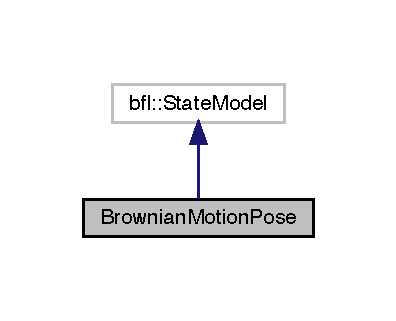
\includegraphics[width=190pt]{classBrownianMotionPose__inherit__graph}
\end{center}
\end{figure}
\subsection*{Public Member Functions}
\begin{DoxyCompactItemize}
\item 
\hyperlink{classBrownianMotionPose_afb57354af3029be488d8416733fbc876}{Brownian\+Motion\+Pose} (const float q\+\_\+xy, const float q\+\_\+z, const float theta, const float cone\+\_\+angle, const unsigned int seed) noexcept
\item 
\hyperlink{classBrownianMotionPose_a033bba640c6452cf0c092abdfa255476}{Brownian\+Motion\+Pose} (const float q\+\_\+xy, const float q\+\_\+z, const float theta, const float cone\+\_\+angle) noexcept
\item 
\hyperlink{classBrownianMotionPose_a042a889f5458b823f067ec600c0ef7b1}{Brownian\+Motion\+Pose} () noexcept
\item 
\hyperlink{classBrownianMotionPose_a0230a822152e6c3f4bc500f86d226b67}{Brownian\+Motion\+Pose} (const \hyperlink{classBrownianMotionPose}{Brownian\+Motion\+Pose} \&bm)
\item 
\hyperlink{classBrownianMotionPose_a5a434f3a0793dd49ea9c4337263636cc}{Brownian\+Motion\+Pose} (\hyperlink{classBrownianMotionPose}{Brownian\+Motion\+Pose} \&\&bm) noexcept
\item 
\hyperlink{classBrownianMotionPose_a12688413184c0b6d757061113a3270db}{$\sim$\+Brownian\+Motion\+Pose} () noexcept
\item 
\hyperlink{classBrownianMotionPose}{Brownian\+Motion\+Pose} \& \hyperlink{classBrownianMotionPose_af57c473922affe4baee38cffe47980d4}{operator=} (const \hyperlink{classBrownianMotionPose}{Brownian\+Motion\+Pose} \&bm)
\item 
\hyperlink{classBrownianMotionPose}{Brownian\+Motion\+Pose} \& \hyperlink{classBrownianMotionPose_a7777bea70e539e180c4748e1e0d50f6e}{operator=} (\hyperlink{classBrownianMotionPose}{Brownian\+Motion\+Pose} \&\&bm) noexcept
\item 
void \hyperlink{classBrownianMotionPose_ac598d506c496740d111ff9ceb4a97459}{propagate} (const Eigen\+::\+Ref$<$ const Eigen\+::\+Matrix\+Xf $>$ \&cur\+\_\+state, Eigen\+::\+Ref$<$ Eigen\+::\+Matrix\+Xf $>$ prop\+\_\+state) override
\item 
void \hyperlink{classBrownianMotionPose_ab1587dfdc83f92d0def84de227d90ddb}{motion} (const Eigen\+::\+Ref$<$ const Eigen\+::\+Matrix\+Xf $>$ \&cur\+\_\+state, Eigen\+::\+Ref$<$ Eigen\+::\+Matrix\+Xf $>$ mot\+\_\+state) override
\item 
Eigen\+::\+Matrix\+Xf \hyperlink{classBrownianMotionPose_a51407ee62d9e384af89c88c5b21c82df}{get\+Noise\+Sample} (const int num) override
\item 
Eigen\+::\+Matrix\+Xf \hyperlink{classBrownianMotionPose_a9b008d4c1b94154a9997454d74eaef88}{get\+Noise\+Covariance\+Matrix} () override
\item 
bool \hyperlink{classBrownianMotionPose_a22ec27f2c6b1c7899a331bbb9390c468}{set\+Property} (const std\+::string \&property) override
\end{DoxyCompactItemize}
\subsection*{Protected Member Functions}
\begin{DoxyCompactItemize}
\item 
void \hyperlink{classBrownianMotionPose_ad5da23c2e31dd9522115ae925a35e66e}{add\+Axisangle\+Disturbance} (const Eigen\+::\+Ref$<$ const Eigen\+::\+Matrix\+Xf $>$ \&disturbance\+\_\+vec, Eigen\+::\+Ref$<$ Eigen\+::\+Matrix\+Xf $>$ current\+\_\+vec)
\end{DoxyCompactItemize}
\subsection*{Protected Attributes}
\begin{DoxyCompactItemize}
\item 
float \hyperlink{classBrownianMotionPose_ac457166961355c8073b93e616ec80741}{q\+\_\+xy\+\_\+}
\item 
float \hyperlink{classBrownianMotionPose_ac5c6eb8bc9bbd4a2e2fb4a70d89c3c8d}{q\+\_\+z\+\_\+}
\item 
float \hyperlink{classBrownianMotionPose_a708069c13925ecb0d11a58519948bf1b}{theta\+\_\+}
\item 
float \hyperlink{classBrownianMotionPose_af1034131a88f7af082bc57eb22d036d5}{cone\+\_\+angle\+\_\+}
\item 
Eigen\+::\+Vector4f \hyperlink{classBrownianMotionPose_a9b58ff8fe85e0fda78a48e4df3fccce0}{cone\+\_\+dir\+\_\+}
\item 
std\+::mt19937\+\_\+64 \hyperlink{classBrownianMotionPose_adf2ae882f026fc526fc29e065bd94162}{generator\+\_\+}
\item 
std\+::normal\+\_\+distribution$<$ float $>$ \hyperlink{classBrownianMotionPose_aa9e8e055568eef783491b424ceb54c37}{distribution\+\_\+pos\+\_\+xy\+\_\+}
\item 
std\+::normal\+\_\+distribution$<$ float $>$ \hyperlink{classBrownianMotionPose_af6c2e7851b82a082e2a5e6885ba93dea}{distribution\+\_\+pos\+\_\+z\+\_\+}
\item 
std\+::normal\+\_\+distribution$<$ float $>$ \hyperlink{classBrownianMotionPose_afc3109f6d9c6b677f4720fb87a2ea51b}{distribution\+\_\+theta\+\_\+}
\item 
std\+::uniform\+\_\+real\+\_\+distribution$<$ float $>$ \hyperlink{classBrownianMotionPose_ad63f33718f94018f88908bb0d661a4e1}{distribution\+\_\+cone\+\_\+}
\item 
std\+::function$<$ float()$>$ \hyperlink{classBrownianMotionPose_a3b9538edc2fe02b6ec1621b8f65d47d9}{gaussian\+\_\+random\+\_\+pos\+\_\+xy\+\_\+}
\item 
std\+::function$<$ float()$>$ \hyperlink{classBrownianMotionPose_ab1115a94b9b81cb8aa746327086d72ca}{gaussian\+\_\+random\+\_\+pos\+\_\+z\+\_\+}
\item 
std\+::function$<$ float()$>$ \hyperlink{classBrownianMotionPose_ab4b2cafbf5d974432290016236946356}{gaussian\+\_\+random\+\_\+theta\+\_\+}
\item 
std\+::function$<$ float()$>$ \hyperlink{classBrownianMotionPose_a7381aa317a5f4b3fe5420d9b67a09b48}{gaussian\+\_\+random\+\_\+cone\+\_\+}
\end{DoxyCompactItemize}


\subsection{Detailed Description}


Definition at line 10 of file Brownian\+Motion\+Pose.\+h.



\subsection{Constructor \& Destructor Documentation}
\mbox{\Hypertarget{classBrownianMotionPose_afb57354af3029be488d8416733fbc876}\label{classBrownianMotionPose_afb57354af3029be488d8416733fbc876}} 
\index{Brownian\+Motion\+Pose@{Brownian\+Motion\+Pose}!Brownian\+Motion\+Pose@{Brownian\+Motion\+Pose}}
\index{Brownian\+Motion\+Pose@{Brownian\+Motion\+Pose}!Brownian\+Motion\+Pose@{Brownian\+Motion\+Pose}}
\subsubsection{\texorpdfstring{Brownian\+Motion\+Pose()}{BrownianMotionPose()}\hspace{0.1cm}{\footnotesize\ttfamily [1/5]}}
{\footnotesize\ttfamily Brownian\+Motion\+Pose\+::\+Brownian\+Motion\+Pose (\begin{DoxyParamCaption}\item[{const float}]{q\+\_\+xy,  }\item[{const float}]{q\+\_\+z,  }\item[{const float}]{theta,  }\item[{const float}]{cone\+\_\+angle,  }\item[{const unsigned int}]{seed }\end{DoxyParamCaption})\hspace{0.3cm}{\ttfamily [noexcept]}}



Definition at line 10 of file Brownian\+Motion\+Pose.\+cpp.

\mbox{\Hypertarget{classBrownianMotionPose_a033bba640c6452cf0c092abdfa255476}\label{classBrownianMotionPose_a033bba640c6452cf0c092abdfa255476}} 
\index{Brownian\+Motion\+Pose@{Brownian\+Motion\+Pose}!Brownian\+Motion\+Pose@{Brownian\+Motion\+Pose}}
\index{Brownian\+Motion\+Pose@{Brownian\+Motion\+Pose}!Brownian\+Motion\+Pose@{Brownian\+Motion\+Pose}}
\subsubsection{\texorpdfstring{Brownian\+Motion\+Pose()}{BrownianMotionPose()}\hspace{0.1cm}{\footnotesize\ttfamily [2/5]}}
{\footnotesize\ttfamily Brownian\+Motion\+Pose\+::\+Brownian\+Motion\+Pose (\begin{DoxyParamCaption}\item[{const float}]{q\+\_\+xy,  }\item[{const float}]{q\+\_\+z,  }\item[{const float}]{theta,  }\item[{const float}]{cone\+\_\+angle }\end{DoxyParamCaption})\hspace{0.3cm}{\ttfamily [noexcept]}}



Definition at line 27 of file Brownian\+Motion\+Pose.\+cpp.

\mbox{\Hypertarget{classBrownianMotionPose_a042a889f5458b823f067ec600c0ef7b1}\label{classBrownianMotionPose_a042a889f5458b823f067ec600c0ef7b1}} 
\index{Brownian\+Motion\+Pose@{Brownian\+Motion\+Pose}!Brownian\+Motion\+Pose@{Brownian\+Motion\+Pose}}
\index{Brownian\+Motion\+Pose@{Brownian\+Motion\+Pose}!Brownian\+Motion\+Pose@{Brownian\+Motion\+Pose}}
\subsubsection{\texorpdfstring{Brownian\+Motion\+Pose()}{BrownianMotionPose()}\hspace{0.1cm}{\footnotesize\ttfamily [3/5]}}
{\footnotesize\ttfamily Brownian\+Motion\+Pose\+::\+Brownian\+Motion\+Pose (\begin{DoxyParamCaption}{ }\end{DoxyParamCaption})\hspace{0.3cm}{\ttfamily [noexcept]}}



Definition at line 31 of file Brownian\+Motion\+Pose.\+cpp.

\mbox{\Hypertarget{classBrownianMotionPose_a0230a822152e6c3f4bc500f86d226b67}\label{classBrownianMotionPose_a0230a822152e6c3f4bc500f86d226b67}} 
\index{Brownian\+Motion\+Pose@{Brownian\+Motion\+Pose}!Brownian\+Motion\+Pose@{Brownian\+Motion\+Pose}}
\index{Brownian\+Motion\+Pose@{Brownian\+Motion\+Pose}!Brownian\+Motion\+Pose@{Brownian\+Motion\+Pose}}
\subsubsection{\texorpdfstring{Brownian\+Motion\+Pose()}{BrownianMotionPose()}\hspace{0.1cm}{\footnotesize\ttfamily [4/5]}}
{\footnotesize\ttfamily Brownian\+Motion\+Pose\+::\+Brownian\+Motion\+Pose (\begin{DoxyParamCaption}\item[{const \hyperlink{classBrownianMotionPose}{Brownian\+Motion\+Pose} \&}]{bm }\end{DoxyParamCaption})}



Definition at line 35 of file Brownian\+Motion\+Pose.\+cpp.

\mbox{\Hypertarget{classBrownianMotionPose_a5a434f3a0793dd49ea9c4337263636cc}\label{classBrownianMotionPose_a5a434f3a0793dd49ea9c4337263636cc}} 
\index{Brownian\+Motion\+Pose@{Brownian\+Motion\+Pose}!Brownian\+Motion\+Pose@{Brownian\+Motion\+Pose}}
\index{Brownian\+Motion\+Pose@{Brownian\+Motion\+Pose}!Brownian\+Motion\+Pose@{Brownian\+Motion\+Pose}}
\subsubsection{\texorpdfstring{Brownian\+Motion\+Pose()}{BrownianMotionPose()}\hspace{0.1cm}{\footnotesize\ttfamily [5/5]}}
{\footnotesize\ttfamily Brownian\+Motion\+Pose\+::\+Brownian\+Motion\+Pose (\begin{DoxyParamCaption}\item[{\hyperlink{classBrownianMotionPose}{Brownian\+Motion\+Pose} \&\&}]{bm }\end{DoxyParamCaption})\hspace{0.3cm}{\ttfamily [noexcept]}}



Definition at line 52 of file Brownian\+Motion\+Pose.\+cpp.

\mbox{\Hypertarget{classBrownianMotionPose_a12688413184c0b6d757061113a3270db}\label{classBrownianMotionPose_a12688413184c0b6d757061113a3270db}} 
\index{Brownian\+Motion\+Pose@{Brownian\+Motion\+Pose}!````~Brownian\+Motion\+Pose@{$\sim$\+Brownian\+Motion\+Pose}}
\index{````~Brownian\+Motion\+Pose@{$\sim$\+Brownian\+Motion\+Pose}!Brownian\+Motion\+Pose@{Brownian\+Motion\+Pose}}
\subsubsection{\texorpdfstring{$\sim$\+Brownian\+Motion\+Pose()}{~BrownianMotionPose()}}
{\footnotesize\ttfamily Brownian\+Motion\+Pose\+::$\sim$\+Brownian\+Motion\+Pose (\begin{DoxyParamCaption}{ }\end{DoxyParamCaption})\hspace{0.3cm}{\ttfamily [noexcept]}}



Definition at line 74 of file Brownian\+Motion\+Pose.\+cpp.



\subsection{Member Function Documentation}
\mbox{\Hypertarget{classBrownianMotionPose_ad5da23c2e31dd9522115ae925a35e66e}\label{classBrownianMotionPose_ad5da23c2e31dd9522115ae925a35e66e}} 
\index{Brownian\+Motion\+Pose@{Brownian\+Motion\+Pose}!add\+Axisangle\+Disturbance@{add\+Axisangle\+Disturbance}}
\index{add\+Axisangle\+Disturbance@{add\+Axisangle\+Disturbance}!Brownian\+Motion\+Pose@{Brownian\+Motion\+Pose}}
\subsubsection{\texorpdfstring{add\+Axisangle\+Disturbance()}{addAxisangleDisturbance()}}
{\footnotesize\ttfamily void Brownian\+Motion\+Pose\+::add\+Axisangle\+Disturbance (\begin{DoxyParamCaption}\item[{const Eigen\+::\+Ref$<$ const Eigen\+::\+Matrix\+Xf $>$ \&}]{disturbance\+\_\+vec,  }\item[{Eigen\+::\+Ref$<$ Eigen\+::\+Matrix\+Xf $>$}]{current\+\_\+vec }\end{DoxyParamCaption})\hspace{0.3cm}{\ttfamily [protected]}}



Definition at line 163 of file Brownian\+Motion\+Pose.\+cpp.



Referenced by motion().

\mbox{\Hypertarget{classBrownianMotionPose_a9b008d4c1b94154a9997454d74eaef88}\label{classBrownianMotionPose_a9b008d4c1b94154a9997454d74eaef88}} 
\index{Brownian\+Motion\+Pose@{Brownian\+Motion\+Pose}!get\+Noise\+Covariance\+Matrix@{get\+Noise\+Covariance\+Matrix}}
\index{get\+Noise\+Covariance\+Matrix@{get\+Noise\+Covariance\+Matrix}!Brownian\+Motion\+Pose@{Brownian\+Motion\+Pose}}
\subsubsection{\texorpdfstring{get\+Noise\+Covariance\+Matrix()}{getNoiseCovarianceMatrix()}}
{\footnotesize\ttfamily Eigen\+::\+Matrix\+Xf Brownian\+Motion\+Pose\+::get\+Noise\+Covariance\+Matrix (\begin{DoxyParamCaption}{ }\end{DoxyParamCaption})\hspace{0.3cm}{\ttfamily [inline]}, {\ttfamily [override]}}



Definition at line 35 of file Brownian\+Motion\+Pose.\+h.

\mbox{\Hypertarget{classBrownianMotionPose_a51407ee62d9e384af89c88c5b21c82df}\label{classBrownianMotionPose_a51407ee62d9e384af89c88c5b21c82df}} 
\index{Brownian\+Motion\+Pose@{Brownian\+Motion\+Pose}!get\+Noise\+Sample@{get\+Noise\+Sample}}
\index{get\+Noise\+Sample@{get\+Noise\+Sample}!Brownian\+Motion\+Pose@{Brownian\+Motion\+Pose}}
\subsubsection{\texorpdfstring{get\+Noise\+Sample()}{getNoiseSample()}}
{\footnotesize\ttfamily Eigen\+::\+Matrix\+Xf Brownian\+Motion\+Pose\+::get\+Noise\+Sample (\begin{DoxyParamCaption}\item[{const int}]{num }\end{DoxyParamCaption})\hspace{0.3cm}{\ttfamily [override]}}



Definition at line 131 of file Brownian\+Motion\+Pose.\+cpp.



References cone\+\_\+angle\+\_\+, gaussian\+\_\+random\+\_\+cone\+\_\+, gaussian\+\_\+random\+\_\+pos\+\_\+xy\+\_\+, gaussian\+\_\+random\+\_\+pos\+\_\+z\+\_\+, and gaussian\+\_\+random\+\_\+theta\+\_\+.



Referenced by motion().

\mbox{\Hypertarget{classBrownianMotionPose_ab1587dfdc83f92d0def84de227d90ddb}\label{classBrownianMotionPose_ab1587dfdc83f92d0def84de227d90ddb}} 
\index{Brownian\+Motion\+Pose@{Brownian\+Motion\+Pose}!motion@{motion}}
\index{motion@{motion}!Brownian\+Motion\+Pose@{Brownian\+Motion\+Pose}}
\subsubsection{\texorpdfstring{motion()}{motion()}}
{\footnotesize\ttfamily void Brownian\+Motion\+Pose\+::motion (\begin{DoxyParamCaption}\item[{const Eigen\+::\+Ref$<$ const Eigen\+::\+Matrix\+Xf $>$ \&}]{cur\+\_\+state,  }\item[{Eigen\+::\+Ref$<$ Eigen\+::\+Matrix\+Xf $>$}]{mot\+\_\+state }\end{DoxyParamCaption})\hspace{0.3cm}{\ttfamily [override]}}



Definition at line 119 of file Brownian\+Motion\+Pose.\+cpp.



References add\+Axisangle\+Disturbance(), get\+Noise\+Sample(), and propagate().

Here is the call graph for this function\+:
\nopagebreak
\begin{figure}[H]
\begin{center}
\leavevmode
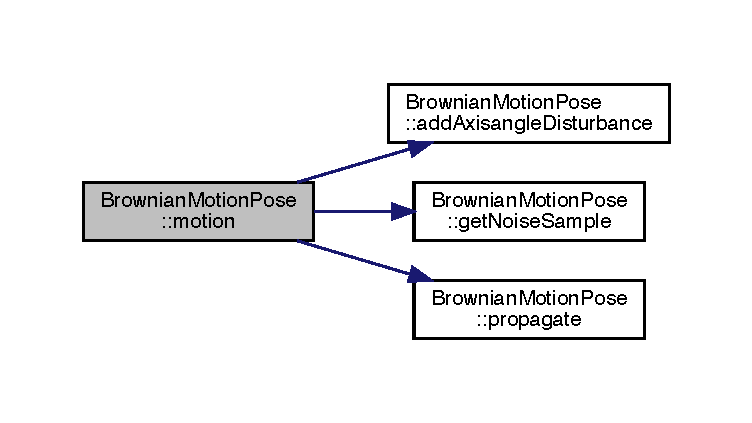
\includegraphics[width=350pt]{classBrownianMotionPose_ab1587dfdc83f92d0def84de227d90ddb_cgraph}
\end{center}
\end{figure}
\mbox{\Hypertarget{classBrownianMotionPose_af57c473922affe4baee38cffe47980d4}\label{classBrownianMotionPose_af57c473922affe4baee38cffe47980d4}} 
\index{Brownian\+Motion\+Pose@{Brownian\+Motion\+Pose}!operator=@{operator=}}
\index{operator=@{operator=}!Brownian\+Motion\+Pose@{Brownian\+Motion\+Pose}}
\subsubsection{\texorpdfstring{operator=()}{operator=()}\hspace{0.1cm}{\footnotesize\ttfamily [1/2]}}
{\footnotesize\ttfamily \hyperlink{classBrownianMotionPose}{Brownian\+Motion\+Pose} \& Brownian\+Motion\+Pose\+::operator= (\begin{DoxyParamCaption}\item[{const \hyperlink{classBrownianMotionPose}{Brownian\+Motion\+Pose} \&}]{bm }\end{DoxyParamCaption})}



Definition at line 77 of file Brownian\+Motion\+Pose.\+cpp.

\mbox{\Hypertarget{classBrownianMotionPose_a7777bea70e539e180c4748e1e0d50f6e}\label{classBrownianMotionPose_a7777bea70e539e180c4748e1e0d50f6e}} 
\index{Brownian\+Motion\+Pose@{Brownian\+Motion\+Pose}!operator=@{operator=}}
\index{operator=@{operator=}!Brownian\+Motion\+Pose@{Brownian\+Motion\+Pose}}
\subsubsection{\texorpdfstring{operator=()}{operator=()}\hspace{0.1cm}{\footnotesize\ttfamily [2/2]}}
{\footnotesize\ttfamily \hyperlink{classBrownianMotionPose}{Brownian\+Motion\+Pose} \& Brownian\+Motion\+Pose\+::operator= (\begin{DoxyParamCaption}\item[{\hyperlink{classBrownianMotionPose}{Brownian\+Motion\+Pose} \&\&}]{bm }\end{DoxyParamCaption})\hspace{0.3cm}{\ttfamily [noexcept]}}



Definition at line 86 of file Brownian\+Motion\+Pose.\+cpp.



References cone\+\_\+angle\+\_\+, cone\+\_\+dir\+\_\+, distribution\+\_\+cone\+\_\+, distribution\+\_\+pos\+\_\+xy\+\_\+, distribution\+\_\+pos\+\_\+z\+\_\+, distribution\+\_\+theta\+\_\+, gaussian\+\_\+random\+\_\+cone\+\_\+, gaussian\+\_\+random\+\_\+pos\+\_\+xy\+\_\+, gaussian\+\_\+random\+\_\+pos\+\_\+z\+\_\+, gaussian\+\_\+random\+\_\+theta\+\_\+, generator\+\_\+, q\+\_\+xy\+\_\+, q\+\_\+z\+\_\+, and theta\+\_\+.

\mbox{\Hypertarget{classBrownianMotionPose_ac598d506c496740d111ff9ceb4a97459}\label{classBrownianMotionPose_ac598d506c496740d111ff9ceb4a97459}} 
\index{Brownian\+Motion\+Pose@{Brownian\+Motion\+Pose}!propagate@{propagate}}
\index{propagate@{propagate}!Brownian\+Motion\+Pose@{Brownian\+Motion\+Pose}}
\subsubsection{\texorpdfstring{propagate()}{propagate()}}
{\footnotesize\ttfamily void Brownian\+Motion\+Pose\+::propagate (\begin{DoxyParamCaption}\item[{const Eigen\+::\+Ref$<$ const Eigen\+::\+Matrix\+Xf $>$ \&}]{cur\+\_\+state,  }\item[{Eigen\+::\+Ref$<$ Eigen\+::\+Matrix\+Xf $>$}]{prop\+\_\+state }\end{DoxyParamCaption})\hspace{0.3cm}{\ttfamily [override]}}



Definition at line 113 of file Brownian\+Motion\+Pose.\+cpp.



Referenced by motion().

\mbox{\Hypertarget{classBrownianMotionPose_a22ec27f2c6b1c7899a331bbb9390c468}\label{classBrownianMotionPose_a22ec27f2c6b1c7899a331bbb9390c468}} 
\index{Brownian\+Motion\+Pose@{Brownian\+Motion\+Pose}!set\+Property@{set\+Property}}
\index{set\+Property@{set\+Property}!Brownian\+Motion\+Pose@{Brownian\+Motion\+Pose}}
\subsubsection{\texorpdfstring{set\+Property()}{setProperty()}}
{\footnotesize\ttfamily bool Brownian\+Motion\+Pose\+::set\+Property (\begin{DoxyParamCaption}\item[{const std\+::string \&}]{property }\end{DoxyParamCaption})\hspace{0.3cm}{\ttfamily [inline]}, {\ttfamily [override]}}



Definition at line 37 of file Brownian\+Motion\+Pose.\+h.



References q\+\_\+xy\+\_\+.



\subsection{Member Data Documentation}
\mbox{\Hypertarget{classBrownianMotionPose_af1034131a88f7af082bc57eb22d036d5}\label{classBrownianMotionPose_af1034131a88f7af082bc57eb22d036d5}} 
\index{Brownian\+Motion\+Pose@{Brownian\+Motion\+Pose}!cone\+\_\+angle\+\_\+@{cone\+\_\+angle\+\_\+}}
\index{cone\+\_\+angle\+\_\+@{cone\+\_\+angle\+\_\+}!Brownian\+Motion\+Pose@{Brownian\+Motion\+Pose}}
\subsubsection{\texorpdfstring{cone\+\_\+angle\+\_\+}{cone\_angle\_}}
{\footnotesize\ttfamily float Brownian\+Motion\+Pose\+::cone\+\_\+angle\+\_\+\hspace{0.3cm}{\ttfamily [protected]}}



Definition at line 43 of file Brownian\+Motion\+Pose.\+h.



Referenced by get\+Noise\+Sample(), and operator=().

\mbox{\Hypertarget{classBrownianMotionPose_a9b58ff8fe85e0fda78a48e4df3fccce0}\label{classBrownianMotionPose_a9b58ff8fe85e0fda78a48e4df3fccce0}} 
\index{Brownian\+Motion\+Pose@{Brownian\+Motion\+Pose}!cone\+\_\+dir\+\_\+@{cone\+\_\+dir\+\_\+}}
\index{cone\+\_\+dir\+\_\+@{cone\+\_\+dir\+\_\+}!Brownian\+Motion\+Pose@{Brownian\+Motion\+Pose}}
\subsubsection{\texorpdfstring{cone\+\_\+dir\+\_\+}{cone\_dir\_}}
{\footnotesize\ttfamily Eigen\+::\+Vector4f Brownian\+Motion\+Pose\+::cone\+\_\+dir\+\_\+\hspace{0.3cm}{\ttfamily [protected]}}



Definition at line 45 of file Brownian\+Motion\+Pose.\+h.



Referenced by operator=().

\mbox{\Hypertarget{classBrownianMotionPose_ad63f33718f94018f88908bb0d661a4e1}\label{classBrownianMotionPose_ad63f33718f94018f88908bb0d661a4e1}} 
\index{Brownian\+Motion\+Pose@{Brownian\+Motion\+Pose}!distribution\+\_\+cone\+\_\+@{distribution\+\_\+cone\+\_\+}}
\index{distribution\+\_\+cone\+\_\+@{distribution\+\_\+cone\+\_\+}!Brownian\+Motion\+Pose@{Brownian\+Motion\+Pose}}
\subsubsection{\texorpdfstring{distribution\+\_\+cone\+\_\+}{distribution\_cone\_}}
{\footnotesize\ttfamily std\+::uniform\+\_\+real\+\_\+distribution$<$float$>$ Brownian\+Motion\+Pose\+::distribution\+\_\+cone\+\_\+\hspace{0.3cm}{\ttfamily [protected]}}



Definition at line 51 of file Brownian\+Motion\+Pose.\+h.



Referenced by operator=().

\mbox{\Hypertarget{classBrownianMotionPose_aa9e8e055568eef783491b424ceb54c37}\label{classBrownianMotionPose_aa9e8e055568eef783491b424ceb54c37}} 
\index{Brownian\+Motion\+Pose@{Brownian\+Motion\+Pose}!distribution\+\_\+pos\+\_\+xy\+\_\+@{distribution\+\_\+pos\+\_\+xy\+\_\+}}
\index{distribution\+\_\+pos\+\_\+xy\+\_\+@{distribution\+\_\+pos\+\_\+xy\+\_\+}!Brownian\+Motion\+Pose@{Brownian\+Motion\+Pose}}
\subsubsection{\texorpdfstring{distribution\+\_\+pos\+\_\+xy\+\_\+}{distribution\_pos\_xy\_}}
{\footnotesize\ttfamily std\+::normal\+\_\+distribution$<$float$>$ Brownian\+Motion\+Pose\+::distribution\+\_\+pos\+\_\+xy\+\_\+\hspace{0.3cm}{\ttfamily [protected]}}



Definition at line 48 of file Brownian\+Motion\+Pose.\+h.



Referenced by operator=().

\mbox{\Hypertarget{classBrownianMotionPose_af6c2e7851b82a082e2a5e6885ba93dea}\label{classBrownianMotionPose_af6c2e7851b82a082e2a5e6885ba93dea}} 
\index{Brownian\+Motion\+Pose@{Brownian\+Motion\+Pose}!distribution\+\_\+pos\+\_\+z\+\_\+@{distribution\+\_\+pos\+\_\+z\+\_\+}}
\index{distribution\+\_\+pos\+\_\+z\+\_\+@{distribution\+\_\+pos\+\_\+z\+\_\+}!Brownian\+Motion\+Pose@{Brownian\+Motion\+Pose}}
\subsubsection{\texorpdfstring{distribution\+\_\+pos\+\_\+z\+\_\+}{distribution\_pos\_z\_}}
{\footnotesize\ttfamily std\+::normal\+\_\+distribution$<$float$>$ Brownian\+Motion\+Pose\+::distribution\+\_\+pos\+\_\+z\+\_\+\hspace{0.3cm}{\ttfamily [protected]}}



Definition at line 49 of file Brownian\+Motion\+Pose.\+h.



Referenced by operator=().

\mbox{\Hypertarget{classBrownianMotionPose_afc3109f6d9c6b677f4720fb87a2ea51b}\label{classBrownianMotionPose_afc3109f6d9c6b677f4720fb87a2ea51b}} 
\index{Brownian\+Motion\+Pose@{Brownian\+Motion\+Pose}!distribution\+\_\+theta\+\_\+@{distribution\+\_\+theta\+\_\+}}
\index{distribution\+\_\+theta\+\_\+@{distribution\+\_\+theta\+\_\+}!Brownian\+Motion\+Pose@{Brownian\+Motion\+Pose}}
\subsubsection{\texorpdfstring{distribution\+\_\+theta\+\_\+}{distribution\_theta\_}}
{\footnotesize\ttfamily std\+::normal\+\_\+distribution$<$float$>$ Brownian\+Motion\+Pose\+::distribution\+\_\+theta\+\_\+\hspace{0.3cm}{\ttfamily [protected]}}



Definition at line 50 of file Brownian\+Motion\+Pose.\+h.



Referenced by operator=().

\mbox{\Hypertarget{classBrownianMotionPose_a7381aa317a5f4b3fe5420d9b67a09b48}\label{classBrownianMotionPose_a7381aa317a5f4b3fe5420d9b67a09b48}} 
\index{Brownian\+Motion\+Pose@{Brownian\+Motion\+Pose}!gaussian\+\_\+random\+\_\+cone\+\_\+@{gaussian\+\_\+random\+\_\+cone\+\_\+}}
\index{gaussian\+\_\+random\+\_\+cone\+\_\+@{gaussian\+\_\+random\+\_\+cone\+\_\+}!Brownian\+Motion\+Pose@{Brownian\+Motion\+Pose}}
\subsubsection{\texorpdfstring{gaussian\+\_\+random\+\_\+cone\+\_\+}{gaussian\_random\_cone\_}}
{\footnotesize\ttfamily std\+::function$<$float()$>$ Brownian\+Motion\+Pose\+::gaussian\+\_\+random\+\_\+cone\+\_\+\hspace{0.3cm}{\ttfamily [protected]}}



Definition at line 55 of file Brownian\+Motion\+Pose.\+h.



Referenced by get\+Noise\+Sample(), and operator=().

\mbox{\Hypertarget{classBrownianMotionPose_a3b9538edc2fe02b6ec1621b8f65d47d9}\label{classBrownianMotionPose_a3b9538edc2fe02b6ec1621b8f65d47d9}} 
\index{Brownian\+Motion\+Pose@{Brownian\+Motion\+Pose}!gaussian\+\_\+random\+\_\+pos\+\_\+xy\+\_\+@{gaussian\+\_\+random\+\_\+pos\+\_\+xy\+\_\+}}
\index{gaussian\+\_\+random\+\_\+pos\+\_\+xy\+\_\+@{gaussian\+\_\+random\+\_\+pos\+\_\+xy\+\_\+}!Brownian\+Motion\+Pose@{Brownian\+Motion\+Pose}}
\subsubsection{\texorpdfstring{gaussian\+\_\+random\+\_\+pos\+\_\+xy\+\_\+}{gaussian\_random\_pos\_xy\_}}
{\footnotesize\ttfamily std\+::function$<$float()$>$ Brownian\+Motion\+Pose\+::gaussian\+\_\+random\+\_\+pos\+\_\+xy\+\_\+\hspace{0.3cm}{\ttfamily [protected]}}



Definition at line 52 of file Brownian\+Motion\+Pose.\+h.



Referenced by get\+Noise\+Sample(), and operator=().

\mbox{\Hypertarget{classBrownianMotionPose_ab1115a94b9b81cb8aa746327086d72ca}\label{classBrownianMotionPose_ab1115a94b9b81cb8aa746327086d72ca}} 
\index{Brownian\+Motion\+Pose@{Brownian\+Motion\+Pose}!gaussian\+\_\+random\+\_\+pos\+\_\+z\+\_\+@{gaussian\+\_\+random\+\_\+pos\+\_\+z\+\_\+}}
\index{gaussian\+\_\+random\+\_\+pos\+\_\+z\+\_\+@{gaussian\+\_\+random\+\_\+pos\+\_\+z\+\_\+}!Brownian\+Motion\+Pose@{Brownian\+Motion\+Pose}}
\subsubsection{\texorpdfstring{gaussian\+\_\+random\+\_\+pos\+\_\+z\+\_\+}{gaussian\_random\_pos\_z\_}}
{\footnotesize\ttfamily std\+::function$<$float()$>$ Brownian\+Motion\+Pose\+::gaussian\+\_\+random\+\_\+pos\+\_\+z\+\_\+\hspace{0.3cm}{\ttfamily [protected]}}



Definition at line 53 of file Brownian\+Motion\+Pose.\+h.



Referenced by get\+Noise\+Sample(), and operator=().

\mbox{\Hypertarget{classBrownianMotionPose_ab4b2cafbf5d974432290016236946356}\label{classBrownianMotionPose_ab4b2cafbf5d974432290016236946356}} 
\index{Brownian\+Motion\+Pose@{Brownian\+Motion\+Pose}!gaussian\+\_\+random\+\_\+theta\+\_\+@{gaussian\+\_\+random\+\_\+theta\+\_\+}}
\index{gaussian\+\_\+random\+\_\+theta\+\_\+@{gaussian\+\_\+random\+\_\+theta\+\_\+}!Brownian\+Motion\+Pose@{Brownian\+Motion\+Pose}}
\subsubsection{\texorpdfstring{gaussian\+\_\+random\+\_\+theta\+\_\+}{gaussian\_random\_theta\_}}
{\footnotesize\ttfamily std\+::function$<$float()$>$ Brownian\+Motion\+Pose\+::gaussian\+\_\+random\+\_\+theta\+\_\+\hspace{0.3cm}{\ttfamily [protected]}}



Definition at line 54 of file Brownian\+Motion\+Pose.\+h.



Referenced by get\+Noise\+Sample(), and operator=().

\mbox{\Hypertarget{classBrownianMotionPose_adf2ae882f026fc526fc29e065bd94162}\label{classBrownianMotionPose_adf2ae882f026fc526fc29e065bd94162}} 
\index{Brownian\+Motion\+Pose@{Brownian\+Motion\+Pose}!generator\+\_\+@{generator\+\_\+}}
\index{generator\+\_\+@{generator\+\_\+}!Brownian\+Motion\+Pose@{Brownian\+Motion\+Pose}}
\subsubsection{\texorpdfstring{generator\+\_\+}{generator\_}}
{\footnotesize\ttfamily std\+::mt19937\+\_\+64 Brownian\+Motion\+Pose\+::generator\+\_\+\hspace{0.3cm}{\ttfamily [protected]}}



Definition at line 47 of file Brownian\+Motion\+Pose.\+h.



Referenced by operator=().

\mbox{\Hypertarget{classBrownianMotionPose_ac457166961355c8073b93e616ec80741}\label{classBrownianMotionPose_ac457166961355c8073b93e616ec80741}} 
\index{Brownian\+Motion\+Pose@{Brownian\+Motion\+Pose}!q\+\_\+xy\+\_\+@{q\+\_\+xy\+\_\+}}
\index{q\+\_\+xy\+\_\+@{q\+\_\+xy\+\_\+}!Brownian\+Motion\+Pose@{Brownian\+Motion\+Pose}}
\subsubsection{\texorpdfstring{q\+\_\+xy\+\_\+}{q\_xy\_}}
{\footnotesize\ttfamily float Brownian\+Motion\+Pose\+::q\+\_\+xy\+\_\+\hspace{0.3cm}{\ttfamily [protected]}}



Definition at line 37 of file Brownian\+Motion\+Pose.\+h.



Referenced by operator=(), and set\+Property().

\mbox{\Hypertarget{classBrownianMotionPose_ac5c6eb8bc9bbd4a2e2fb4a70d89c3c8d}\label{classBrownianMotionPose_ac5c6eb8bc9bbd4a2e2fb4a70d89c3c8d}} 
\index{Brownian\+Motion\+Pose@{Brownian\+Motion\+Pose}!q\+\_\+z\+\_\+@{q\+\_\+z\+\_\+}}
\index{q\+\_\+z\+\_\+@{q\+\_\+z\+\_\+}!Brownian\+Motion\+Pose@{Brownian\+Motion\+Pose}}
\subsubsection{\texorpdfstring{q\+\_\+z\+\_\+}{q\_z\_}}
{\footnotesize\ttfamily float Brownian\+Motion\+Pose\+::q\+\_\+z\+\_\+\hspace{0.3cm}{\ttfamily [protected]}}



Definition at line 41 of file Brownian\+Motion\+Pose.\+h.



Referenced by operator=().

\mbox{\Hypertarget{classBrownianMotionPose_a708069c13925ecb0d11a58519948bf1b}\label{classBrownianMotionPose_a708069c13925ecb0d11a58519948bf1b}} 
\index{Brownian\+Motion\+Pose@{Brownian\+Motion\+Pose}!theta\+\_\+@{theta\+\_\+}}
\index{theta\+\_\+@{theta\+\_\+}!Brownian\+Motion\+Pose@{Brownian\+Motion\+Pose}}
\subsubsection{\texorpdfstring{theta\+\_\+}{theta\_}}
{\footnotesize\ttfamily float Brownian\+Motion\+Pose\+::theta\+\_\+\hspace{0.3cm}{\ttfamily [protected]}}



Definition at line 42 of file Brownian\+Motion\+Pose.\+h.



Referenced by operator=().



The documentation for this class was generated from the following files\+:\begin{DoxyCompactItemize}
\item 
/\+Users/\+Claudio/\+Git\+Hub/visual-\/tracking-\/control/src/hand-\/tracking/include/\hyperlink{BrownianMotionPose_8h}{Brownian\+Motion\+Pose.\+h}\item 
/\+Users/\+Claudio/\+Git\+Hub/visual-\/tracking-\/control/src/hand-\/tracking/src/\hyperlink{BrownianMotionPose_8cpp}{Brownian\+Motion\+Pose.\+cpp}\end{DoxyCompactItemize}

\hypertarget{classbfl_1_1DrawFwdKinPoses}{}\section{bfl\+:\+:Draw\+Fwd\+Kin\+Poses Class Reference}
\label{classbfl_1_1DrawFwdKinPoses}\index{bfl\+::\+Draw\+Fwd\+Kin\+Poses@{bfl\+::\+Draw\+Fwd\+Kin\+Poses}}


{\ttfamily \#include $<$Draw\+Fwd\+Kin\+Poses.\+h$>$}



Inheritance diagram for bfl\+:\+:Draw\+Fwd\+Kin\+Poses\+:
\nopagebreak
\begin{figure}[H]
\begin{center}
\leavevmode
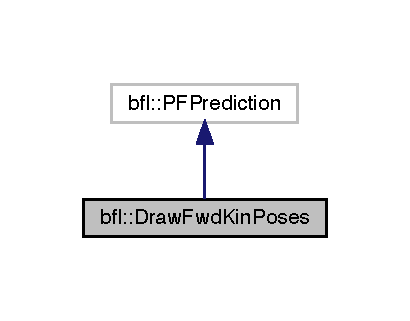
\includegraphics[width=197pt]{classbfl_1_1DrawFwdKinPoses__inherit__graph}
\end{center}
\end{figure}
\subsection*{Public Member Functions}
\begin{DoxyCompactItemize}
\item 
\hyperlink{classbfl_1_1DrawFwdKinPoses_a76ac04c55f02309c5724c22694a591c9}{Draw\+Fwd\+Kin\+Poses} () noexcept
\item 
\hyperlink{classbfl_1_1DrawFwdKinPoses_a558686870e99ef9941d9e709a80ecfcc}{Draw\+Fwd\+Kin\+Poses} (\hyperlink{classbfl_1_1DrawFwdKinPoses}{Draw\+Fwd\+Kin\+Poses} \&\&pf\+\_\+prediction) noexcept
\item 
\hyperlink{classbfl_1_1DrawFwdKinPoses_a8c9122942a30efa9e4c31704293d4932}{$\sim$\+Draw\+Fwd\+Kin\+Poses} () noexcept
\item 
\hyperlink{classbfl_1_1DrawFwdKinPoses}{Draw\+Fwd\+Kin\+Poses} \& \hyperlink{classbfl_1_1DrawFwdKinPoses_af3c60f95018e80c15816c0e7ec4b75c7}{operator=} (\hyperlink{classbfl_1_1DrawFwdKinPoses}{Draw\+Fwd\+Kin\+Poses} \&\&pf\+\_\+prediction) noexcept
\item 
State\+Model \& \hyperlink{classbfl_1_1DrawFwdKinPoses_a3273b9ac31c6a5cec5a3d76a498b82b8}{get\+State\+Model} () override
\item 
void \hyperlink{classbfl_1_1DrawFwdKinPoses_ad416d76778dd76e0b16c07cd7fb30b7b}{set\+State\+Model} (std\+::unique\+\_\+ptr$<$ State\+Model $>$ state\+\_\+model) override
\item 
Exogenous\+Model \& \hyperlink{classbfl_1_1DrawFwdKinPoses_a97ad3a63a71ca40e193d0d18e5faf539}{get\+Exogenous\+Model} () override
\item 
void \hyperlink{classbfl_1_1DrawFwdKinPoses_ad42f7b9870d3f38faa439acc0bd793c7}{set\+Exogenous\+Model} (std\+::unique\+\_\+ptr$<$ Exogenous\+Model $>$ exogenous\+\_\+model) override
\end{DoxyCompactItemize}
\subsection*{Protected Member Functions}
\begin{DoxyCompactItemize}
\item 
void \hyperlink{classbfl_1_1DrawFwdKinPoses_a2b2766e81769769fb299f31f644d1761}{predict\+Step} (const Eigen\+::\+Ref$<$ const Eigen\+::\+Matrix\+Xf $>$ \&prev\+\_\+states, const Eigen\+::\+Ref$<$ const Eigen\+::\+Vector\+Xf $>$ \&prev\+\_\+weights, Eigen\+::\+Ref$<$ Eigen\+::\+Matrix\+Xf $>$ pred\+\_\+states, Eigen\+::\+Ref$<$ Eigen\+::\+Vector\+Xf $>$ pred\+\_\+weights) override
\end{DoxyCompactItemize}
\subsection*{Protected Attributes}
\begin{DoxyCompactItemize}
\item 
std\+::unique\+\_\+ptr$<$ State\+Model $>$ \hyperlink{classbfl_1_1DrawFwdKinPoses_afcd1bf7246acdc971075b8ba63f8986a}{state\+\_\+model\+\_\+}
\item 
std\+::unique\+\_\+ptr$<$ Exogenous\+Model $>$ \hyperlink{classbfl_1_1DrawFwdKinPoses_af5fcf31aeb103a36830fc8363039540b}{exogenous\+\_\+model\+\_\+}
\end{DoxyCompactItemize}


\subsection{Detailed Description}


Definition at line 15 of file Draw\+Fwd\+Kin\+Poses.\+h.



\subsection{Constructor \& Destructor Documentation}
\mbox{\Hypertarget{classbfl_1_1DrawFwdKinPoses_a76ac04c55f02309c5724c22694a591c9}\label{classbfl_1_1DrawFwdKinPoses_a76ac04c55f02309c5724c22694a591c9}} 
\index{bfl\+::\+Draw\+Fwd\+Kin\+Poses@{bfl\+::\+Draw\+Fwd\+Kin\+Poses}!Draw\+Fwd\+Kin\+Poses@{Draw\+Fwd\+Kin\+Poses}}
\index{Draw\+Fwd\+Kin\+Poses@{Draw\+Fwd\+Kin\+Poses}!bfl\+::\+Draw\+Fwd\+Kin\+Poses@{bfl\+::\+Draw\+Fwd\+Kin\+Poses}}
\subsubsection{\texorpdfstring{Draw\+Fwd\+Kin\+Poses()}{DrawFwdKinPoses()}\hspace{0.1cm}{\footnotesize\ttfamily [1/2]}}
{\footnotesize\ttfamily Draw\+Fwd\+Kin\+Poses\+::\+Draw\+Fwd\+Kin\+Poses (\begin{DoxyParamCaption}{ }\end{DoxyParamCaption})\hspace{0.3cm}{\ttfamily [noexcept]}}



Definition at line 9 of file Draw\+Fwd\+Kin\+Poses.\+cpp.

\mbox{\Hypertarget{classbfl_1_1DrawFwdKinPoses_a558686870e99ef9941d9e709a80ecfcc}\label{classbfl_1_1DrawFwdKinPoses_a558686870e99ef9941d9e709a80ecfcc}} 
\index{bfl\+::\+Draw\+Fwd\+Kin\+Poses@{bfl\+::\+Draw\+Fwd\+Kin\+Poses}!Draw\+Fwd\+Kin\+Poses@{Draw\+Fwd\+Kin\+Poses}}
\index{Draw\+Fwd\+Kin\+Poses@{Draw\+Fwd\+Kin\+Poses}!bfl\+::\+Draw\+Fwd\+Kin\+Poses@{bfl\+::\+Draw\+Fwd\+Kin\+Poses}}
\subsubsection{\texorpdfstring{Draw\+Fwd\+Kin\+Poses()}{DrawFwdKinPoses()}\hspace{0.1cm}{\footnotesize\ttfamily [2/2]}}
{\footnotesize\ttfamily Draw\+Fwd\+Kin\+Poses\+::\+Draw\+Fwd\+Kin\+Poses (\begin{DoxyParamCaption}\item[{\hyperlink{classbfl_1_1DrawFwdKinPoses}{Draw\+Fwd\+Kin\+Poses} \&\&}]{pf\+\_\+prediction }\end{DoxyParamCaption})\hspace{0.3cm}{\ttfamily [noexcept]}}



Definition at line 15 of file Draw\+Fwd\+Kin\+Poses.\+cpp.

\mbox{\Hypertarget{classbfl_1_1DrawFwdKinPoses_a8c9122942a30efa9e4c31704293d4932}\label{classbfl_1_1DrawFwdKinPoses_a8c9122942a30efa9e4c31704293d4932}} 
\index{bfl\+::\+Draw\+Fwd\+Kin\+Poses@{bfl\+::\+Draw\+Fwd\+Kin\+Poses}!````~Draw\+Fwd\+Kin\+Poses@{$\sim$\+Draw\+Fwd\+Kin\+Poses}}
\index{````~Draw\+Fwd\+Kin\+Poses@{$\sim$\+Draw\+Fwd\+Kin\+Poses}!bfl\+::\+Draw\+Fwd\+Kin\+Poses@{bfl\+::\+Draw\+Fwd\+Kin\+Poses}}
\subsubsection{\texorpdfstring{$\sim$\+Draw\+Fwd\+Kin\+Poses()}{~DrawFwdKinPoses()}}
{\footnotesize\ttfamily Draw\+Fwd\+Kin\+Poses\+::$\sim$\+Draw\+Fwd\+Kin\+Poses (\begin{DoxyParamCaption}{ }\end{DoxyParamCaption})\hspace{0.3cm}{\ttfamily [noexcept]}}



Definition at line 12 of file Draw\+Fwd\+Kin\+Poses.\+cpp.



\subsection{Member Function Documentation}
\mbox{\Hypertarget{classbfl_1_1DrawFwdKinPoses_a97ad3a63a71ca40e193d0d18e5faf539}\label{classbfl_1_1DrawFwdKinPoses_a97ad3a63a71ca40e193d0d18e5faf539}} 
\index{bfl\+::\+Draw\+Fwd\+Kin\+Poses@{bfl\+::\+Draw\+Fwd\+Kin\+Poses}!get\+Exogenous\+Model@{get\+Exogenous\+Model}}
\index{get\+Exogenous\+Model@{get\+Exogenous\+Model}!bfl\+::\+Draw\+Fwd\+Kin\+Poses@{bfl\+::\+Draw\+Fwd\+Kin\+Poses}}
\subsubsection{\texorpdfstring{get\+Exogenous\+Model()}{getExogenousModel()}}
{\footnotesize\ttfamily Exogenous\+Model \& Draw\+Fwd\+Kin\+Poses\+::get\+Exogenous\+Model (\begin{DoxyParamCaption}{ }\end{DoxyParamCaption})\hspace{0.3cm}{\ttfamily [override]}}



Definition at line 42 of file Draw\+Fwd\+Kin\+Poses.\+cpp.

\mbox{\Hypertarget{classbfl_1_1DrawFwdKinPoses_a3273b9ac31c6a5cec5a3d76a498b82b8}\label{classbfl_1_1DrawFwdKinPoses_a3273b9ac31c6a5cec5a3d76a498b82b8}} 
\index{bfl\+::\+Draw\+Fwd\+Kin\+Poses@{bfl\+::\+Draw\+Fwd\+Kin\+Poses}!get\+State\+Model@{get\+State\+Model}}
\index{get\+State\+Model@{get\+State\+Model}!bfl\+::\+Draw\+Fwd\+Kin\+Poses@{bfl\+::\+Draw\+Fwd\+Kin\+Poses}}
\subsubsection{\texorpdfstring{get\+State\+Model()}{getStateModel()}}
{\footnotesize\ttfamily State\+Model \& Draw\+Fwd\+Kin\+Poses\+::get\+State\+Model (\begin{DoxyParamCaption}{ }\end{DoxyParamCaption})\hspace{0.3cm}{\ttfamily [override]}}



Definition at line 30 of file Draw\+Fwd\+Kin\+Poses.\+cpp.

\mbox{\Hypertarget{classbfl_1_1DrawFwdKinPoses_af3c60f95018e80c15816c0e7ec4b75c7}\label{classbfl_1_1DrawFwdKinPoses_af3c60f95018e80c15816c0e7ec4b75c7}} 
\index{bfl\+::\+Draw\+Fwd\+Kin\+Poses@{bfl\+::\+Draw\+Fwd\+Kin\+Poses}!operator=@{operator=}}
\index{operator=@{operator=}!bfl\+::\+Draw\+Fwd\+Kin\+Poses@{bfl\+::\+Draw\+Fwd\+Kin\+Poses}}
\subsubsection{\texorpdfstring{operator=()}{operator=()}}
{\footnotesize\ttfamily \hyperlink{classbfl_1_1DrawFwdKinPoses}{Draw\+Fwd\+Kin\+Poses} \& Draw\+Fwd\+Kin\+Poses\+::operator= (\begin{DoxyParamCaption}\item[{\hyperlink{classbfl_1_1DrawFwdKinPoses}{Draw\+Fwd\+Kin\+Poses} \&\&}]{pf\+\_\+prediction }\end{DoxyParamCaption})\hspace{0.3cm}{\ttfamily [noexcept]}}



Definition at line 20 of file Draw\+Fwd\+Kin\+Poses.\+cpp.

\mbox{\Hypertarget{classbfl_1_1DrawFwdKinPoses_a2b2766e81769769fb299f31f644d1761}\label{classbfl_1_1DrawFwdKinPoses_a2b2766e81769769fb299f31f644d1761}} 
\index{bfl\+::\+Draw\+Fwd\+Kin\+Poses@{bfl\+::\+Draw\+Fwd\+Kin\+Poses}!predict\+Step@{predict\+Step}}
\index{predict\+Step@{predict\+Step}!bfl\+::\+Draw\+Fwd\+Kin\+Poses@{bfl\+::\+Draw\+Fwd\+Kin\+Poses}}
\subsubsection{\texorpdfstring{predict\+Step()}{predictStep()}}
{\footnotesize\ttfamily void Draw\+Fwd\+Kin\+Poses\+::predict\+Step (\begin{DoxyParamCaption}\item[{const Eigen\+::\+Ref$<$ const Eigen\+::\+Matrix\+Xf $>$ \&}]{prev\+\_\+states,  }\item[{const Eigen\+::\+Ref$<$ const Eigen\+::\+Vector\+Xf $>$ \&}]{prev\+\_\+weights,  }\item[{Eigen\+::\+Ref$<$ Eigen\+::\+Matrix\+Xf $>$}]{pred\+\_\+states,  }\item[{Eigen\+::\+Ref$<$ Eigen\+::\+Vector\+Xf $>$}]{pred\+\_\+weights }\end{DoxyParamCaption})\hspace{0.3cm}{\ttfamily [override]}, {\ttfamily [protected]}}



Definition at line 54 of file Draw\+Fwd\+Kin\+Poses.\+cpp.

\mbox{\Hypertarget{classbfl_1_1DrawFwdKinPoses_ad42f7b9870d3f38faa439acc0bd793c7}\label{classbfl_1_1DrawFwdKinPoses_ad42f7b9870d3f38faa439acc0bd793c7}} 
\index{bfl\+::\+Draw\+Fwd\+Kin\+Poses@{bfl\+::\+Draw\+Fwd\+Kin\+Poses}!set\+Exogenous\+Model@{set\+Exogenous\+Model}}
\index{set\+Exogenous\+Model@{set\+Exogenous\+Model}!bfl\+::\+Draw\+Fwd\+Kin\+Poses@{bfl\+::\+Draw\+Fwd\+Kin\+Poses}}
\subsubsection{\texorpdfstring{set\+Exogenous\+Model()}{setExogenousModel()}}
{\footnotesize\ttfamily void Draw\+Fwd\+Kin\+Poses\+::set\+Exogenous\+Model (\begin{DoxyParamCaption}\item[{std\+::unique\+\_\+ptr$<$ Exogenous\+Model $>$}]{exogenous\+\_\+model }\end{DoxyParamCaption})\hspace{0.3cm}{\ttfamily [override]}}



Definition at line 48 of file Draw\+Fwd\+Kin\+Poses.\+cpp.

\mbox{\Hypertarget{classbfl_1_1DrawFwdKinPoses_ad416d76778dd76e0b16c07cd7fb30b7b}\label{classbfl_1_1DrawFwdKinPoses_ad416d76778dd76e0b16c07cd7fb30b7b}} 
\index{bfl\+::\+Draw\+Fwd\+Kin\+Poses@{bfl\+::\+Draw\+Fwd\+Kin\+Poses}!set\+State\+Model@{set\+State\+Model}}
\index{set\+State\+Model@{set\+State\+Model}!bfl\+::\+Draw\+Fwd\+Kin\+Poses@{bfl\+::\+Draw\+Fwd\+Kin\+Poses}}
\subsubsection{\texorpdfstring{set\+State\+Model()}{setStateModel()}}
{\footnotesize\ttfamily void Draw\+Fwd\+Kin\+Poses\+::set\+State\+Model (\begin{DoxyParamCaption}\item[{std\+::unique\+\_\+ptr$<$ State\+Model $>$}]{state\+\_\+model }\end{DoxyParamCaption})\hspace{0.3cm}{\ttfamily [override]}}



Definition at line 36 of file Draw\+Fwd\+Kin\+Poses.\+cpp.



\subsection{Member Data Documentation}
\mbox{\Hypertarget{classbfl_1_1DrawFwdKinPoses_af5fcf31aeb103a36830fc8363039540b}\label{classbfl_1_1DrawFwdKinPoses_af5fcf31aeb103a36830fc8363039540b}} 
\index{bfl\+::\+Draw\+Fwd\+Kin\+Poses@{bfl\+::\+Draw\+Fwd\+Kin\+Poses}!exogenous\+\_\+model\+\_\+@{exogenous\+\_\+model\+\_\+}}
\index{exogenous\+\_\+model\+\_\+@{exogenous\+\_\+model\+\_\+}!bfl\+::\+Draw\+Fwd\+Kin\+Poses@{bfl\+::\+Draw\+Fwd\+Kin\+Poses}}
\subsubsection{\texorpdfstring{exogenous\+\_\+model\+\_\+}{exogenous\_model\_}}
{\footnotesize\ttfamily std\+::unique\+\_\+ptr$<$Exogenous\+Model$>$ bfl\+::\+Draw\+Fwd\+Kin\+Poses\+::exogenous\+\_\+model\+\_\+\hspace{0.3cm}{\ttfamily [protected]}}



Definition at line 41 of file Draw\+Fwd\+Kin\+Poses.\+h.

\mbox{\Hypertarget{classbfl_1_1DrawFwdKinPoses_afcd1bf7246acdc971075b8ba63f8986a}\label{classbfl_1_1DrawFwdKinPoses_afcd1bf7246acdc971075b8ba63f8986a}} 
\index{bfl\+::\+Draw\+Fwd\+Kin\+Poses@{bfl\+::\+Draw\+Fwd\+Kin\+Poses}!state\+\_\+model\+\_\+@{state\+\_\+model\+\_\+}}
\index{state\+\_\+model\+\_\+@{state\+\_\+model\+\_\+}!bfl\+::\+Draw\+Fwd\+Kin\+Poses@{bfl\+::\+Draw\+Fwd\+Kin\+Poses}}
\subsubsection{\texorpdfstring{state\+\_\+model\+\_\+}{state\_model\_}}
{\footnotesize\ttfamily std\+::unique\+\_\+ptr$<$State\+Model$>$ bfl\+::\+Draw\+Fwd\+Kin\+Poses\+::state\+\_\+model\+\_\+\hspace{0.3cm}{\ttfamily [protected]}}



Definition at line 39 of file Draw\+Fwd\+Kin\+Poses.\+h.



The documentation for this class was generated from the following files\+:\begin{DoxyCompactItemize}
\item 
/\+Users/\+Claudio/\+Git\+Hub/visual-\/tracking-\/control/src/hand-\/tracking/include/\hyperlink{DrawFwdKinPoses_8h}{Draw\+Fwd\+Kin\+Poses.\+h}\item 
/\+Users/\+Claudio/\+Git\+Hub/visual-\/tracking-\/control/src/hand-\/tracking/src/\hyperlink{DrawFwdKinPoses_8cpp}{Draw\+Fwd\+Kin\+Poses.\+cpp}\end{DoxyCompactItemize}

\hypertarget{classFwdKinModel}{}\section{Fwd\+Kin\+Model Class Reference}
\label{classFwdKinModel}\index{Fwd\+Kin\+Model@{Fwd\+Kin\+Model}}


{\ttfamily \#include $<$Fwd\+Kin\+Model.\+h$>$}



Inheritance diagram for Fwd\+Kin\+Model\+:
\nopagebreak
\begin{figure}[H]
\begin{center}
\leavevmode
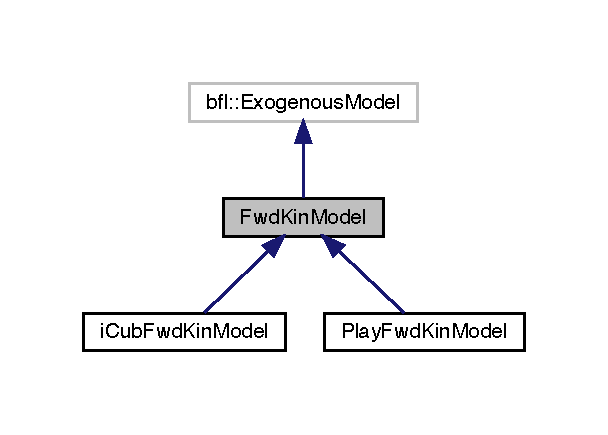
\includegraphics[width=292pt]{classFwdKinModel__inherit__graph}
\end{center}
\end{figure}
\subsection*{Public Member Functions}
\begin{DoxyCompactItemize}
\item 
\hyperlink{classFwdKinModel_aff57436563440b831b701b7b9633ab9b}{Fwd\+Kin\+Model} () noexcept
\item 
\hyperlink{classFwdKinModel_afb77abf94a9f8b8379b6e71b4ca0f3c1}{$\sim$\+Fwd\+Kin\+Model} () noexcept
\item 
void \hyperlink{classFwdKinModel_a9461ff14a1ae8d05169e8f1c7a6237c7}{propagate} (const Eigen\+::\+Ref$<$ const Eigen\+::\+Matrix\+Xf $>$ \&cur\+\_\+state, Eigen\+::\+Ref$<$ Eigen\+::\+Matrix\+Xf $>$ prop\+\_\+state) override
\item 
Eigen\+::\+Matrix\+Xf \hyperlink{classFwdKinModel_ac8ed4e8a52f5ff33cc158c80c6cf083e}{get\+Exogenous\+Matrix} () override
\item 
bool \hyperlink{classFwdKinModel_ae5515e8bb1ebc936f67851a796b75fe1}{set\+Property} (const std\+::string \&property) override
\end{DoxyCompactItemize}
\subsection*{Protected Member Functions}
\begin{DoxyCompactItemize}
\item 
virtual Eigen\+::\+Vector\+Xd \hyperlink{classFwdKinModel_aaad9ff96f725fc529672e12aed86dc02}{read\+Pose} ()=0
\item 
bool \hyperlink{classFwdKinModel_a12b54bd62ba5cf218973c600c66ba39e}{set\+Delta\+Motion} ()
\end{DoxyCompactItemize}
\subsection*{Protected Attributes}
\begin{DoxyCompactItemize}
\item 
bool \hyperlink{classFwdKinModel_a2ed7b77ebd710e5debe63b83a34a1645}{initialize\+\_\+delta\+\_\+} = true
\end{DoxyCompactItemize}
\subsection*{Private Attributes}
\begin{DoxyCompactItemize}
\item 
Eigen\+::\+Vector\+Xd \hyperlink{classFwdKinModel_a45262d07057de0c165eae2d425890505}{prev\+\_\+ee\+\_\+pose\+\_\+} = Eigen\+::\+Vector\+Xd\+::\+Zero(7)
\item 
Eigen\+::\+Vector\+Xd \hyperlink{classFwdKinModel_a508ba314e35ba5ce3efb4a48d76e7fa0}{delta\+\_\+hand\+\_\+pose\+\_\+} = Eigen\+::\+Vector\+Xd\+::\+Zero(6)
\item 
double \hyperlink{classFwdKinModel_a17b3e7f99cfdfdc9890ff81d1a162e7e}{delta\+\_\+angle\+\_\+} = 0.\+0
\end{DoxyCompactItemize}


\subsection{Detailed Description}


Definition at line 12 of file Fwd\+Kin\+Model.\+h.



\subsection{Constructor \& Destructor Documentation}
\mbox{\Hypertarget{classFwdKinModel_aff57436563440b831b701b7b9633ab9b}\label{classFwdKinModel_aff57436563440b831b701b7b9633ab9b}} 
\index{Fwd\+Kin\+Model@{Fwd\+Kin\+Model}!Fwd\+Kin\+Model@{Fwd\+Kin\+Model}}
\index{Fwd\+Kin\+Model@{Fwd\+Kin\+Model}!Fwd\+Kin\+Model@{Fwd\+Kin\+Model}}
\subsubsection{\texorpdfstring{Fwd\+Kin\+Model()}{FwdKinModel()}}
{\footnotesize\ttfamily Fwd\+Kin\+Model\+::\+Fwd\+Kin\+Model (\begin{DoxyParamCaption}{ }\end{DoxyParamCaption})\hspace{0.3cm}{\ttfamily [noexcept]}}



Definition at line 22 of file Fwd\+Kin\+Model.\+cpp.

\mbox{\Hypertarget{classFwdKinModel_afb77abf94a9f8b8379b6e71b4ca0f3c1}\label{classFwdKinModel_afb77abf94a9f8b8379b6e71b4ca0f3c1}} 
\index{Fwd\+Kin\+Model@{Fwd\+Kin\+Model}!````~Fwd\+Kin\+Model@{$\sim$\+Fwd\+Kin\+Model}}
\index{````~Fwd\+Kin\+Model@{$\sim$\+Fwd\+Kin\+Model}!Fwd\+Kin\+Model@{Fwd\+Kin\+Model}}
\subsubsection{\texorpdfstring{$\sim$\+Fwd\+Kin\+Model()}{~FwdKinModel()}}
{\footnotesize\ttfamily Fwd\+Kin\+Model\+::$\sim$\+Fwd\+Kin\+Model (\begin{DoxyParamCaption}{ }\end{DoxyParamCaption})\hspace{0.3cm}{\ttfamily [noexcept]}}



Definition at line 25 of file Fwd\+Kin\+Model.\+cpp.



\subsection{Member Function Documentation}
\mbox{\Hypertarget{classFwdKinModel_ac8ed4e8a52f5ff33cc158c80c6cf083e}\label{classFwdKinModel_ac8ed4e8a52f5ff33cc158c80c6cf083e}} 
\index{Fwd\+Kin\+Model@{Fwd\+Kin\+Model}!get\+Exogenous\+Matrix@{get\+Exogenous\+Matrix}}
\index{get\+Exogenous\+Matrix@{get\+Exogenous\+Matrix}!Fwd\+Kin\+Model@{Fwd\+Kin\+Model}}
\subsubsection{\texorpdfstring{get\+Exogenous\+Matrix()}{getExogenousMatrix()}}
{\footnotesize\ttfamily Matrix\+Xf Fwd\+Kin\+Model\+::get\+Exogenous\+Matrix (\begin{DoxyParamCaption}{ }\end{DoxyParamCaption})\hspace{0.3cm}{\ttfamily [override]}}



Definition at line 47 of file Fwd\+Kin\+Model.\+cpp.

\mbox{\Hypertarget{classFwdKinModel_a9461ff14a1ae8d05169e8f1c7a6237c7}\label{classFwdKinModel_a9461ff14a1ae8d05169e8f1c7a6237c7}} 
\index{Fwd\+Kin\+Model@{Fwd\+Kin\+Model}!propagate@{propagate}}
\index{propagate@{propagate}!Fwd\+Kin\+Model@{Fwd\+Kin\+Model}}
\subsubsection{\texorpdfstring{propagate()}{propagate()}}
{\footnotesize\ttfamily void Fwd\+Kin\+Model\+::propagate (\begin{DoxyParamCaption}\item[{const Eigen\+::\+Ref$<$ const Eigen\+::\+Matrix\+Xf $>$ \&}]{cur\+\_\+state,  }\item[{Eigen\+::\+Ref$<$ Eigen\+::\+Matrix\+Xf $>$}]{prop\+\_\+state }\end{DoxyParamCaption})\hspace{0.3cm}{\ttfamily [override]}}



Definition at line 28 of file Fwd\+Kin\+Model.\+cpp.

\mbox{\Hypertarget{classFwdKinModel_aaad9ff96f725fc529672e12aed86dc02}\label{classFwdKinModel_aaad9ff96f725fc529672e12aed86dc02}} 
\index{Fwd\+Kin\+Model@{Fwd\+Kin\+Model}!read\+Pose@{read\+Pose}}
\index{read\+Pose@{read\+Pose}!Fwd\+Kin\+Model@{Fwd\+Kin\+Model}}
\subsubsection{\texorpdfstring{read\+Pose()}{readPose()}}
{\footnotesize\ttfamily virtual Eigen\+::\+Vector\+Xd Fwd\+Kin\+Model\+::read\+Pose (\begin{DoxyParamCaption}{ }\end{DoxyParamCaption})\hspace{0.3cm}{\ttfamily [protected]}, {\ttfamily [pure virtual]}}



Implemented in \hyperlink{classiCubFwdKinModel_ad549519048e9b54c18af51c6b173b726}{i\+Cub\+Fwd\+Kin\+Model}, and \hyperlink{classPlayFwdKinModel_a282700bc69b26e6ea28cc5048881a599}{Play\+Fwd\+Kin\+Model}.

\mbox{\Hypertarget{classFwdKinModel_a12b54bd62ba5cf218973c600c66ba39e}\label{classFwdKinModel_a12b54bd62ba5cf218973c600c66ba39e}} 
\index{Fwd\+Kin\+Model@{Fwd\+Kin\+Model}!set\+Delta\+Motion@{set\+Delta\+Motion}}
\index{set\+Delta\+Motion@{set\+Delta\+Motion}!Fwd\+Kin\+Model@{Fwd\+Kin\+Model}}
\subsubsection{\texorpdfstring{set\+Delta\+Motion()}{setDeltaMotion()}}
{\footnotesize\ttfamily bool Fwd\+Kin\+Model\+::set\+Delta\+Motion (\begin{DoxyParamCaption}{ }\end{DoxyParamCaption})\hspace{0.3cm}{\ttfamily [protected]}}



Definition at line 71 of file Fwd\+Kin\+Model.\+cpp.

\mbox{\Hypertarget{classFwdKinModel_ae5515e8bb1ebc936f67851a796b75fe1}\label{classFwdKinModel_ae5515e8bb1ebc936f67851a796b75fe1}} 
\index{Fwd\+Kin\+Model@{Fwd\+Kin\+Model}!set\+Property@{set\+Property}}
\index{set\+Property@{set\+Property}!Fwd\+Kin\+Model@{Fwd\+Kin\+Model}}
\subsubsection{\texorpdfstring{set\+Property()}{setProperty()}}
{\footnotesize\ttfamily bool Fwd\+Kin\+Model\+::set\+Property (\begin{DoxyParamCaption}\item[{const std\+::string \&}]{property }\end{DoxyParamCaption})\hspace{0.3cm}{\ttfamily [override]}}



Definition at line 56 of file Fwd\+Kin\+Model.\+cpp.



Referenced by i\+Cub\+Fwd\+Kin\+Model\+::set\+Property(), and Play\+Fwd\+Kin\+Model\+::set\+Property().



\subsection{Member Data Documentation}
\mbox{\Hypertarget{classFwdKinModel_a17b3e7f99cfdfdc9890ff81d1a162e7e}\label{classFwdKinModel_a17b3e7f99cfdfdc9890ff81d1a162e7e}} 
\index{Fwd\+Kin\+Model@{Fwd\+Kin\+Model}!delta\+\_\+angle\+\_\+@{delta\+\_\+angle\+\_\+}}
\index{delta\+\_\+angle\+\_\+@{delta\+\_\+angle\+\_\+}!Fwd\+Kin\+Model@{Fwd\+Kin\+Model}}
\subsubsection{\texorpdfstring{delta\+\_\+angle\+\_\+}{delta\_angle\_}}
{\footnotesize\ttfamily double Fwd\+Kin\+Model\+::delta\+\_\+angle\+\_\+ = 0.\+0\hspace{0.3cm}{\ttfamily [private]}}



Definition at line 34 of file Fwd\+Kin\+Model.\+h.

\mbox{\Hypertarget{classFwdKinModel_a508ba314e35ba5ce3efb4a48d76e7fa0}\label{classFwdKinModel_a508ba314e35ba5ce3efb4a48d76e7fa0}} 
\index{Fwd\+Kin\+Model@{Fwd\+Kin\+Model}!delta\+\_\+hand\+\_\+pose\+\_\+@{delta\+\_\+hand\+\_\+pose\+\_\+}}
\index{delta\+\_\+hand\+\_\+pose\+\_\+@{delta\+\_\+hand\+\_\+pose\+\_\+}!Fwd\+Kin\+Model@{Fwd\+Kin\+Model}}
\subsubsection{\texorpdfstring{delta\+\_\+hand\+\_\+pose\+\_\+}{delta\_hand\_pose\_}}
{\footnotesize\ttfamily Eigen\+::\+Vector\+Xd Fwd\+Kin\+Model\+::delta\+\_\+hand\+\_\+pose\+\_\+ = Eigen\+::\+Vector\+Xd\+::\+Zero(6)\hspace{0.3cm}{\ttfamily [private]}}



Definition at line 33 of file Fwd\+Kin\+Model.\+h.

\mbox{\Hypertarget{classFwdKinModel_a2ed7b77ebd710e5debe63b83a34a1645}\label{classFwdKinModel_a2ed7b77ebd710e5debe63b83a34a1645}} 
\index{Fwd\+Kin\+Model@{Fwd\+Kin\+Model}!initialize\+\_\+delta\+\_\+@{initialize\+\_\+delta\+\_\+}}
\index{initialize\+\_\+delta\+\_\+@{initialize\+\_\+delta\+\_\+}!Fwd\+Kin\+Model@{Fwd\+Kin\+Model}}
\subsubsection{\texorpdfstring{initialize\+\_\+delta\+\_\+}{initialize\_delta\_}}
{\footnotesize\ttfamily bool Fwd\+Kin\+Model\+::initialize\+\_\+delta\+\_\+ = true\hspace{0.3cm}{\ttfamily [protected]}}



Definition at line 28 of file Fwd\+Kin\+Model.\+h.

\mbox{\Hypertarget{classFwdKinModel_a45262d07057de0c165eae2d425890505}\label{classFwdKinModel_a45262d07057de0c165eae2d425890505}} 
\index{Fwd\+Kin\+Model@{Fwd\+Kin\+Model}!prev\+\_\+ee\+\_\+pose\+\_\+@{prev\+\_\+ee\+\_\+pose\+\_\+}}
\index{prev\+\_\+ee\+\_\+pose\+\_\+@{prev\+\_\+ee\+\_\+pose\+\_\+}!Fwd\+Kin\+Model@{Fwd\+Kin\+Model}}
\subsubsection{\texorpdfstring{prev\+\_\+ee\+\_\+pose\+\_\+}{prev\_ee\_pose\_}}
{\footnotesize\ttfamily Eigen\+::\+Vector\+Xd Fwd\+Kin\+Model\+::prev\+\_\+ee\+\_\+pose\+\_\+ = Eigen\+::\+Vector\+Xd\+::\+Zero(7)\hspace{0.3cm}{\ttfamily [private]}}



Definition at line 32 of file Fwd\+Kin\+Model.\+h.



The documentation for this class was generated from the following files\+:\begin{DoxyCompactItemize}
\item 
/\+Users/\+Claudio/\+Git\+Hub/visual-\/tracking-\/control/src/hand-\/tracking/include/\hyperlink{FwdKinModel_8h}{Fwd\+Kin\+Model.\+h}\item 
/\+Users/\+Claudio/\+Git\+Hub/visual-\/tracking-\/control/src/hand-\/tracking/src/\hyperlink{FwdKinModel_8cpp}{Fwd\+Kin\+Model.\+cpp}\end{DoxyCompactItemize}

\hypertarget{classGatePose}{}\section{Gate\+Pose Class Reference}
\label{classGatePose}\index{Gate\+Pose@{Gate\+Pose}}


{\ttfamily \#include $<$Gate\+Pose.\+h$>$}



Inheritance diagram for Gate\+Pose\+:
\nopagebreak
\begin{figure}[H]
\begin{center}
\leavevmode
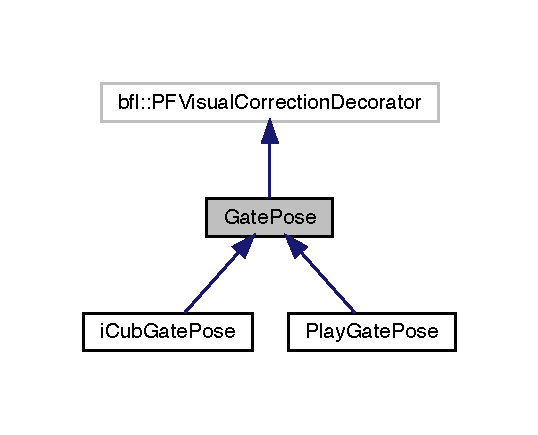
\includegraphics[width=258pt]{classGatePose__inherit__graph}
\end{center}
\end{figure}
\subsection*{Public Member Functions}
\begin{DoxyCompactItemize}
\item 
\hyperlink{classGatePose_a27001df58131fc1431f1a3d768698494}{Gate\+Pose} (std\+::unique\+\_\+ptr$<$ P\+F\+Visual\+Correction $>$ visual\+\_\+correction, const double gate\+\_\+x, const double gate\+\_\+y, const double gate\+\_\+z, const double gate\+\_\+rotation, const double gate\+\_\+aperture) noexcept
\item 
\hyperlink{classGatePose_a27e224f41699efe5949e2fb876b1d9ee}{Gate\+Pose} (std\+::unique\+\_\+ptr$<$ P\+F\+Visual\+Correction $>$ visual\+\_\+correction) noexcept
\item 
\hyperlink{classGatePose_acea85773116a379f108b7c53152d9420}{$\sim$\+Gate\+Pose} () noexcept
\item 
void \hyperlink{classGatePose_a00607a4325dcfb7a02bda7490b65d25c}{innovation} (const Eigen\+::\+Ref$<$ const Eigen\+::\+Matrix\+Xf $>$ \&pred\+\_\+states, cv\+::\+Input\+Array measurements, Eigen\+::\+Ref$<$ Eigen\+::\+Matrix\+Xf $>$ innovations) override
\item 
double \hyperlink{classGatePose_a939c575d5d59c8b0f3ab528edd368c0d}{likelihood} (const Eigen\+::\+Ref$<$ const Eigen\+::\+Matrix\+Xf $>$ \&innovations) override
\item 
bfl\+::\+Visual\+Observation\+Model \& \hyperlink{classGatePose_aa47f9242f039b8752675db5594350a28}{get\+Visual\+Observation\+Model} () override
\item 
void \hyperlink{classGatePose_a18ba358c801ae1a246dbee2f9780c698}{set\+Visual\+Observation\+Model} (std\+::unique\+\_\+ptr$<$ bfl\+::\+Visual\+Observation\+Model $>$ visual\+\_\+observation\+\_\+model) override
\end{DoxyCompactItemize}
\subsection*{Protected Member Functions}
\begin{DoxyCompactItemize}
\item 
void \hyperlink{classGatePose_a91d395abe75dc7772116f50219dc19ae}{correct\+Step} (const Eigen\+::\+Ref$<$ const Eigen\+::\+Matrix\+Xf $>$ \&pred\+\_\+states, const Eigen\+::\+Ref$<$ const Eigen\+::\+Vector\+Xf $>$ \&pred\+\_\+weights, cv\+::\+Input\+Array measurements, Eigen\+::\+Ref$<$ Eigen\+::\+Matrix\+Xf $>$ cor\+\_\+states, Eigen\+::\+Ref$<$ Eigen\+::\+Vector\+Xf $>$ cor\+\_\+weights) override
\item 
virtual Eigen\+::\+Vector\+Xd \hyperlink{classGatePose_aed9235df850c3ca930f9e43276bf4f62}{read\+Pose} ()=0
\item 
bool \hyperlink{classGatePose_a880273787b1b3542e1e7971954ac118d}{is\+Inside\+Ellipsoid} (const Eigen\+::\+Ref$<$ const Eigen\+::\+Vector\+Xf $>$ \&state)
\item 
bool \hyperlink{classGatePose_a6d188756ed5dcc56c311a2aafc9d1acd}{is\+Within\+Rotation} (float rot\+\_\+angle)
\item 
bool \hyperlink{classGatePose_ad2e8708b3ed5a8252bdec1494f199fda}{is\+Inside\+Cone} (const Eigen\+::\+Ref$<$ const Eigen\+::\+Vector\+Xf $>$ \&state)
\end{DoxyCompactItemize}
\subsection*{Private Attributes}
\begin{DoxyCompactItemize}
\item 
double \hyperlink{classGatePose_a702b2c10eb1d86b9a0ac139b3f894310}{gate\+\_\+x\+\_\+}
\item 
double \hyperlink{classGatePose_a844864ec9133c4c2081b3682ca243cac}{gate\+\_\+y\+\_\+}
\item 
double \hyperlink{classGatePose_a1ff2edfa464cfe7efc8c1da43f59de21}{gate\+\_\+z\+\_\+}
\item 
double \hyperlink{classGatePose_ac5e580554426053ea164e00fbe41f775}{gate\+\_\+aperture\+\_\+}
\item 
double \hyperlink{classGatePose_a98dd62845368c46900f7cf0dcac358e5}{gate\+\_\+rotation\+\_\+}
\item 
Eigen\+::\+Vector\+Xd \hyperlink{classGatePose_affa53c9f133bf1dd59de8880317cf3cd}{ee\+\_\+pose\+\_\+}
\end{DoxyCompactItemize}


\subsection{Detailed Description}


Definition at line 10 of file Gate\+Pose.\+h.



\subsection{Constructor \& Destructor Documentation}
\mbox{\Hypertarget{classGatePose_a27001df58131fc1431f1a3d768698494}\label{classGatePose_a27001df58131fc1431f1a3d768698494}} 
\index{Gate\+Pose@{Gate\+Pose}!Gate\+Pose@{Gate\+Pose}}
\index{Gate\+Pose@{Gate\+Pose}!Gate\+Pose@{Gate\+Pose}}
\subsubsection{\texorpdfstring{Gate\+Pose()}{GatePose()}\hspace{0.1cm}{\footnotesize\ttfamily [1/2]}}
{\footnotesize\ttfamily Gate\+Pose\+::\+Gate\+Pose (\begin{DoxyParamCaption}\item[{std\+::unique\+\_\+ptr$<$ P\+F\+Visual\+Correction $>$}]{visual\+\_\+correction,  }\item[{const double}]{gate\+\_\+x,  }\item[{const double}]{gate\+\_\+y,  }\item[{const double}]{gate\+\_\+z,  }\item[{const double}]{gate\+\_\+rotation,  }\item[{const double}]{gate\+\_\+aperture }\end{DoxyParamCaption})\hspace{0.3cm}{\ttfamily [noexcept]}}



Definition at line 10 of file Gate\+Pose.\+cpp.

\mbox{\Hypertarget{classGatePose_a27e224f41699efe5949e2fb876b1d9ee}\label{classGatePose_a27e224f41699efe5949e2fb876b1d9ee}} 
\index{Gate\+Pose@{Gate\+Pose}!Gate\+Pose@{Gate\+Pose}}
\index{Gate\+Pose@{Gate\+Pose}!Gate\+Pose@{Gate\+Pose}}
\subsubsection{\texorpdfstring{Gate\+Pose()}{GatePose()}\hspace{0.1cm}{\footnotesize\ttfamily [2/2]}}
{\footnotesize\ttfamily Gate\+Pose\+::\+Gate\+Pose (\begin{DoxyParamCaption}\item[{std\+::unique\+\_\+ptr$<$ P\+F\+Visual\+Correction $>$}]{visual\+\_\+correction }\end{DoxyParamCaption})\hspace{0.3cm}{\ttfamily [noexcept]}}



Definition at line 23 of file Gate\+Pose.\+cpp.

\mbox{\Hypertarget{classGatePose_acea85773116a379f108b7c53152d9420}\label{classGatePose_acea85773116a379f108b7c53152d9420}} 
\index{Gate\+Pose@{Gate\+Pose}!````~Gate\+Pose@{$\sim$\+Gate\+Pose}}
\index{````~Gate\+Pose@{$\sim$\+Gate\+Pose}!Gate\+Pose@{Gate\+Pose}}
\subsubsection{\texorpdfstring{$\sim$\+Gate\+Pose()}{~GatePose()}}
{\footnotesize\ttfamily Gate\+Pose\+::$\sim$\+Gate\+Pose (\begin{DoxyParamCaption}{ }\end{DoxyParamCaption})\hspace{0.3cm}{\ttfamily [noexcept]}}



Definition at line 27 of file Gate\+Pose.\+cpp.



\subsection{Member Function Documentation}
\mbox{\Hypertarget{classGatePose_a91d395abe75dc7772116f50219dc19ae}\label{classGatePose_a91d395abe75dc7772116f50219dc19ae}} 
\index{Gate\+Pose@{Gate\+Pose}!correct\+Step@{correct\+Step}}
\index{correct\+Step@{correct\+Step}!Gate\+Pose@{Gate\+Pose}}
\subsubsection{\texorpdfstring{correct\+Step()}{correctStep()}}
{\footnotesize\ttfamily void Gate\+Pose\+::correct\+Step (\begin{DoxyParamCaption}\item[{const Eigen\+::\+Ref$<$ const Eigen\+::\+Matrix\+Xf $>$ \&}]{pred\+\_\+states,  }\item[{const Eigen\+::\+Ref$<$ const Eigen\+::\+Vector\+Xf $>$ \&}]{pred\+\_\+weights,  }\item[{cv\+::\+Input\+Array}]{measurements,  }\item[{Eigen\+::\+Ref$<$ Eigen\+::\+Matrix\+Xf $>$}]{cor\+\_\+states,  }\item[{Eigen\+::\+Ref$<$ Eigen\+::\+Vector\+Xf $>$}]{cor\+\_\+weights }\end{DoxyParamCaption})\hspace{0.3cm}{\ttfamily [override]}, {\ttfamily [protected]}}



Definition at line 54 of file Gate\+Pose.\+cpp.

\mbox{\Hypertarget{classGatePose_aa47f9242f039b8752675db5594350a28}\label{classGatePose_aa47f9242f039b8752675db5594350a28}} 
\index{Gate\+Pose@{Gate\+Pose}!get\+Visual\+Observation\+Model@{get\+Visual\+Observation\+Model}}
\index{get\+Visual\+Observation\+Model@{get\+Visual\+Observation\+Model}!Gate\+Pose@{Gate\+Pose}}
\subsubsection{\texorpdfstring{get\+Visual\+Observation\+Model()}{getVisualObservationModel()}}
{\footnotesize\ttfamily Visual\+Observation\+Model \& Gate\+Pose\+::get\+Visual\+Observation\+Model (\begin{DoxyParamCaption}{ }\end{DoxyParamCaption})\hspace{0.3cm}{\ttfamily [override]}}



Definition at line 42 of file Gate\+Pose.\+cpp.

\mbox{\Hypertarget{classGatePose_a00607a4325dcfb7a02bda7490b65d25c}\label{classGatePose_a00607a4325dcfb7a02bda7490b65d25c}} 
\index{Gate\+Pose@{Gate\+Pose}!innovation@{innovation}}
\index{innovation@{innovation}!Gate\+Pose@{Gate\+Pose}}
\subsubsection{\texorpdfstring{innovation()}{innovation()}}
{\footnotesize\ttfamily void Gate\+Pose\+::innovation (\begin{DoxyParamCaption}\item[{const Eigen\+::\+Ref$<$ const Eigen\+::\+Matrix\+Xf $>$ \&}]{pred\+\_\+states,  }\item[{cv\+::\+Input\+Array}]{measurements,  }\item[{Eigen\+::\+Ref$<$ Eigen\+::\+Matrix\+Xf $>$}]{innovations }\end{DoxyParamCaption})\hspace{0.3cm}{\ttfamily [override]}}



Definition at line 30 of file Gate\+Pose.\+cpp.

\mbox{\Hypertarget{classGatePose_ad2e8708b3ed5a8252bdec1494f199fda}\label{classGatePose_ad2e8708b3ed5a8252bdec1494f199fda}} 
\index{Gate\+Pose@{Gate\+Pose}!is\+Inside\+Cone@{is\+Inside\+Cone}}
\index{is\+Inside\+Cone@{is\+Inside\+Cone}!Gate\+Pose@{Gate\+Pose}}
\subsubsection{\texorpdfstring{is\+Inside\+Cone()}{isInsideCone()}}
{\footnotesize\ttfamily bool Gate\+Pose\+::is\+Inside\+Cone (\begin{DoxyParamCaption}\item[{const Eigen\+::\+Ref$<$ const Eigen\+::\+Vector\+Xf $>$ \&}]{state }\end{DoxyParamCaption})\hspace{0.3cm}{\ttfamily [protected]}}



Definition at line 88 of file Gate\+Pose.\+cpp.

\mbox{\Hypertarget{classGatePose_a880273787b1b3542e1e7971954ac118d}\label{classGatePose_a880273787b1b3542e1e7971954ac118d}} 
\index{Gate\+Pose@{Gate\+Pose}!is\+Inside\+Ellipsoid@{is\+Inside\+Ellipsoid}}
\index{is\+Inside\+Ellipsoid@{is\+Inside\+Ellipsoid}!Gate\+Pose@{Gate\+Pose}}
\subsubsection{\texorpdfstring{is\+Inside\+Ellipsoid()}{isInsideEllipsoid()}}
{\footnotesize\ttfamily bool Gate\+Pose\+::is\+Inside\+Ellipsoid (\begin{DoxyParamCaption}\item[{const Eigen\+::\+Ref$<$ const Eigen\+::\+Vector\+Xf $>$ \&}]{state }\end{DoxyParamCaption})\hspace{0.3cm}{\ttfamily [protected]}}



Definition at line 72 of file Gate\+Pose.\+cpp.

\mbox{\Hypertarget{classGatePose_a6d188756ed5dcc56c311a2aafc9d1acd}\label{classGatePose_a6d188756ed5dcc56c311a2aafc9d1acd}} 
\index{Gate\+Pose@{Gate\+Pose}!is\+Within\+Rotation@{is\+Within\+Rotation}}
\index{is\+Within\+Rotation@{is\+Within\+Rotation}!Gate\+Pose@{Gate\+Pose}}
\subsubsection{\texorpdfstring{is\+Within\+Rotation()}{isWithinRotation()}}
{\footnotesize\ttfamily bool Gate\+Pose\+::is\+Within\+Rotation (\begin{DoxyParamCaption}\item[{float}]{rot\+\_\+angle }\end{DoxyParamCaption})\hspace{0.3cm}{\ttfamily [protected]}}



Definition at line 80 of file Gate\+Pose.\+cpp.

\mbox{\Hypertarget{classGatePose_a939c575d5d59c8b0f3ab528edd368c0d}\label{classGatePose_a939c575d5d59c8b0f3ab528edd368c0d}} 
\index{Gate\+Pose@{Gate\+Pose}!likelihood@{likelihood}}
\index{likelihood@{likelihood}!Gate\+Pose@{Gate\+Pose}}
\subsubsection{\texorpdfstring{likelihood()}{likelihood()}}
{\footnotesize\ttfamily double Gate\+Pose\+::likelihood (\begin{DoxyParamCaption}\item[{const Eigen\+::\+Ref$<$ const Eigen\+::\+Matrix\+Xf $>$ \&}]{innovations }\end{DoxyParamCaption})\hspace{0.3cm}{\ttfamily [override]}}



Definition at line 36 of file Gate\+Pose.\+cpp.

\mbox{\Hypertarget{classGatePose_aed9235df850c3ca930f9e43276bf4f62}\label{classGatePose_aed9235df850c3ca930f9e43276bf4f62}} 
\index{Gate\+Pose@{Gate\+Pose}!read\+Pose@{read\+Pose}}
\index{read\+Pose@{read\+Pose}!Gate\+Pose@{Gate\+Pose}}
\subsubsection{\texorpdfstring{read\+Pose()}{readPose()}}
{\footnotesize\ttfamily virtual Eigen\+::\+Vector\+Xd Gate\+Pose\+::read\+Pose (\begin{DoxyParamCaption}{ }\end{DoxyParamCaption})\hspace{0.3cm}{\ttfamily [protected]}, {\ttfamily [pure virtual]}}



Implemented in \hyperlink{classiCubGatePose_aff1494edcf8f17803788f954ba0b443b}{i\+Cub\+Gate\+Pose}, and \hyperlink{classPlayGatePose_a863afa00ea83395e7f2ceffd26242106}{Play\+Gate\+Pose}.

\mbox{\Hypertarget{classGatePose_a18ba358c801ae1a246dbee2f9780c698}\label{classGatePose_a18ba358c801ae1a246dbee2f9780c698}} 
\index{Gate\+Pose@{Gate\+Pose}!set\+Visual\+Observation\+Model@{set\+Visual\+Observation\+Model}}
\index{set\+Visual\+Observation\+Model@{set\+Visual\+Observation\+Model}!Gate\+Pose@{Gate\+Pose}}
\subsubsection{\texorpdfstring{set\+Visual\+Observation\+Model()}{setVisualObservationModel()}}
{\footnotesize\ttfamily void Gate\+Pose\+::set\+Visual\+Observation\+Model (\begin{DoxyParamCaption}\item[{std\+::unique\+\_\+ptr$<$ bfl\+::\+Visual\+Observation\+Model $>$}]{visual\+\_\+observation\+\_\+model }\end{DoxyParamCaption})\hspace{0.3cm}{\ttfamily [override]}}



Definition at line 48 of file Gate\+Pose.\+cpp.



\subsection{Member Data Documentation}
\mbox{\Hypertarget{classGatePose_affa53c9f133bf1dd59de8880317cf3cd}\label{classGatePose_affa53c9f133bf1dd59de8880317cf3cd}} 
\index{Gate\+Pose@{Gate\+Pose}!ee\+\_\+pose\+\_\+@{ee\+\_\+pose\+\_\+}}
\index{ee\+\_\+pose\+\_\+@{ee\+\_\+pose\+\_\+}!Gate\+Pose@{Gate\+Pose}}
\subsubsection{\texorpdfstring{ee\+\_\+pose\+\_\+}{ee\_pose\_}}
{\footnotesize\ttfamily Eigen\+::\+Vector\+Xd Gate\+Pose\+::ee\+\_\+pose\+\_\+\hspace{0.3cm}{\ttfamily [private]}}



Definition at line 49 of file Gate\+Pose.\+h.

\mbox{\Hypertarget{classGatePose_ac5e580554426053ea164e00fbe41f775}\label{classGatePose_ac5e580554426053ea164e00fbe41f775}} 
\index{Gate\+Pose@{Gate\+Pose}!gate\+\_\+aperture\+\_\+@{gate\+\_\+aperture\+\_\+}}
\index{gate\+\_\+aperture\+\_\+@{gate\+\_\+aperture\+\_\+}!Gate\+Pose@{Gate\+Pose}}
\subsubsection{\texorpdfstring{gate\+\_\+aperture\+\_\+}{gate\_aperture\_}}
{\footnotesize\ttfamily double Gate\+Pose\+::gate\+\_\+aperture\+\_\+\hspace{0.3cm}{\ttfamily [private]}}



Definition at line 46 of file Gate\+Pose.\+h.

\mbox{\Hypertarget{classGatePose_a98dd62845368c46900f7cf0dcac358e5}\label{classGatePose_a98dd62845368c46900f7cf0dcac358e5}} 
\index{Gate\+Pose@{Gate\+Pose}!gate\+\_\+rotation\+\_\+@{gate\+\_\+rotation\+\_\+}}
\index{gate\+\_\+rotation\+\_\+@{gate\+\_\+rotation\+\_\+}!Gate\+Pose@{Gate\+Pose}}
\subsubsection{\texorpdfstring{gate\+\_\+rotation\+\_\+}{gate\_rotation\_}}
{\footnotesize\ttfamily double Gate\+Pose\+::gate\+\_\+rotation\+\_\+\hspace{0.3cm}{\ttfamily [private]}}



Definition at line 47 of file Gate\+Pose.\+h.

\mbox{\Hypertarget{classGatePose_a702b2c10eb1d86b9a0ac139b3f894310}\label{classGatePose_a702b2c10eb1d86b9a0ac139b3f894310}} 
\index{Gate\+Pose@{Gate\+Pose}!gate\+\_\+x\+\_\+@{gate\+\_\+x\+\_\+}}
\index{gate\+\_\+x\+\_\+@{gate\+\_\+x\+\_\+}!Gate\+Pose@{Gate\+Pose}}
\subsubsection{\texorpdfstring{gate\+\_\+x\+\_\+}{gate\_x\_}}
{\footnotesize\ttfamily double Gate\+Pose\+::gate\+\_\+x\+\_\+\hspace{0.3cm}{\ttfamily [private]}}



Definition at line 43 of file Gate\+Pose.\+h.

\mbox{\Hypertarget{classGatePose_a844864ec9133c4c2081b3682ca243cac}\label{classGatePose_a844864ec9133c4c2081b3682ca243cac}} 
\index{Gate\+Pose@{Gate\+Pose}!gate\+\_\+y\+\_\+@{gate\+\_\+y\+\_\+}}
\index{gate\+\_\+y\+\_\+@{gate\+\_\+y\+\_\+}!Gate\+Pose@{Gate\+Pose}}
\subsubsection{\texorpdfstring{gate\+\_\+y\+\_\+}{gate\_y\_}}
{\footnotesize\ttfamily double Gate\+Pose\+::gate\+\_\+y\+\_\+\hspace{0.3cm}{\ttfamily [private]}}



Definition at line 44 of file Gate\+Pose.\+h.

\mbox{\Hypertarget{classGatePose_a1ff2edfa464cfe7efc8c1da43f59de21}\label{classGatePose_a1ff2edfa464cfe7efc8c1da43f59de21}} 
\index{Gate\+Pose@{Gate\+Pose}!gate\+\_\+z\+\_\+@{gate\+\_\+z\+\_\+}}
\index{gate\+\_\+z\+\_\+@{gate\+\_\+z\+\_\+}!Gate\+Pose@{Gate\+Pose}}
\subsubsection{\texorpdfstring{gate\+\_\+z\+\_\+}{gate\_z\_}}
{\footnotesize\ttfamily double Gate\+Pose\+::gate\+\_\+z\+\_\+\hspace{0.3cm}{\ttfamily [private]}}



Definition at line 45 of file Gate\+Pose.\+h.



The documentation for this class was generated from the following files\+:\begin{DoxyCompactItemize}
\item 
/\+Users/\+Claudio/\+Git\+Hub/visual-\/tracking-\/control/src/hand-\/tracking/include/\hyperlink{GatePose_8h}{Gate\+Pose.\+h}\item 
/\+Users/\+Claudio/\+Git\+Hub/visual-\/tracking-\/control/src/hand-\/tracking/src/\hyperlink{GatePose_8cpp}{Gate\+Pose.\+cpp}\end{DoxyCompactItemize}

\hypertarget{classiCubFwdKinModel}{}\section{i\+Cub\+Fwd\+Kin\+Model Class Reference}
\label{classiCubFwdKinModel}\index{i\+Cub\+Fwd\+Kin\+Model@{i\+Cub\+Fwd\+Kin\+Model}}


{\ttfamily \#include $<$i\+Cub\+Fwd\+Kin\+Model.\+h$>$}



Inheritance diagram for i\+Cub\+Fwd\+Kin\+Model\+:
\nopagebreak
\begin{figure}[H]
\begin{center}
\leavevmode
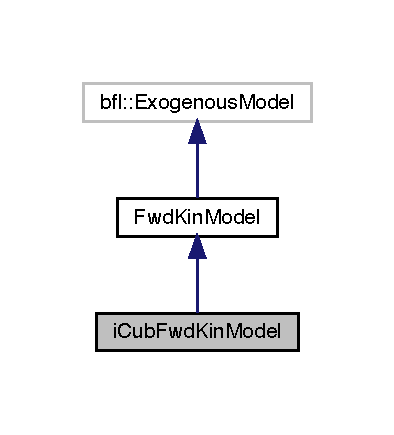
\includegraphics[width=189pt]{classiCubFwdKinModel__inherit__graph}
\end{center}
\end{figure}
\subsection*{Public Member Functions}
\begin{DoxyCompactItemize}
\item 
\hyperlink{classiCubFwdKinModel_a97bd690952f48bb7d7994ff3d2d8b2b9}{i\+Cub\+Fwd\+Kin\+Model} (const yarp\+::os\+::\+Const\+String \&robot, const yarp\+::os\+::\+Const\+String \&laterality, const yarp\+::os\+::\+Const\+String \&port\+\_\+prefix)
\item 
\hyperlink{classiCubFwdKinModel_a60922638092ac5432739602e6541f9e4}{$\sim$i\+Cub\+Fwd\+Kin\+Model} () noexcept
\item 
bool \hyperlink{classiCubFwdKinModel_a2daa3bb3b2c458200dc487ac00929260}{set\+Property} (const std\+::string \&property) override
\item 
void \hyperlink{classFwdKinModel_a9461ff14a1ae8d05169e8f1c7a6237c7}{propagate} (const Eigen\+::\+Ref$<$ const Eigen\+::\+Matrix\+Xf $>$ \&cur\+\_\+state, Eigen\+::\+Ref$<$ Eigen\+::\+Matrix\+Xf $>$ prop\+\_\+state) override
\item 
Eigen\+::\+Matrix\+Xf \hyperlink{classFwdKinModel_ac8ed4e8a52f5ff33cc158c80c6cf083e}{get\+Exogenous\+Matrix} () override
\end{DoxyCompactItemize}
\subsection*{Protected Member Functions}
\begin{DoxyCompactItemize}
\item 
Eigen\+::\+Vector\+Xd \hyperlink{classiCubFwdKinModel_ad549519048e9b54c18af51c6b173b726}{read\+Pose} () override
\item 
yarp\+::sig\+::\+Vector \hyperlink{classiCubFwdKinModel_a4ed6df084a996223a740a7065e16b799}{read\+Torso} ()
\item 
yarp\+::sig\+::\+Vector \hyperlink{classiCubFwdKinModel_a638ea7ef68d98f306346684c93934a93}{read\+Root\+To\+EE} ()
\item 
bool \hyperlink{classFwdKinModel_a12b54bd62ba5cf218973c600c66ba39e}{set\+Delta\+Motion} ()
\end{DoxyCompactItemize}
\subsection*{Protected Attributes}
\begin{DoxyCompactItemize}
\item 
yarp\+::dev\+::\+Poly\+Driver \hyperlink{classiCubFwdKinModel_a3a07f11e9b770e8fc7c03bff05c52927}{drv\+\_\+arm\+\_\+enc\+\_\+}
\item 
yarp\+::dev\+::\+Poly\+Driver \hyperlink{classiCubFwdKinModel_af0ca571291c508a2a058c1ff802e6421}{drv\+\_\+torso\+\_\+enc\+\_\+}
\item 
yarp\+::dev\+::\+I\+Encoders $\ast$ \hyperlink{classiCubFwdKinModel_a4478fa4b4f0689d819a19a5cccd69ae2}{itf\+\_\+arm\+\_\+enc\+\_\+}
\item 
yarp\+::dev\+::\+I\+Encoders $\ast$ \hyperlink{classiCubFwdKinModel_a2d83dd73bf08f66563e9e33d2c26d16a}{itf\+\_\+torso\+\_\+enc\+\_\+}
\item 
i\+Cub\+::i\+Kin\+::i\+Cub\+Arm \hyperlink{classiCubFwdKinModel_a4b92808d2c83eaff8a3bf18dede7001a}{icub\+\_\+kin\+\_\+arm\+\_\+}
\item 
bool \hyperlink{classFwdKinModel_a2ed7b77ebd710e5debe63b83a34a1645}{initialize\+\_\+delta\+\_\+} = true
\end{DoxyCompactItemize}
\subsection*{Private Attributes}
\begin{DoxyCompactItemize}
\item 
yarp\+::os\+::\+Const\+String \hyperlink{classiCubFwdKinModel_a3eb6c400ef775a5549aa31fe22fae4c0}{I\+D\+\_\+} = \char`\"{}i\+Cub\+Fwd\+Kin\+Model\char`\"{}
\item 
yarp\+::os\+::\+Const\+String \hyperlink{classiCubFwdKinModel_a091abb2a5386537d63a67fbf761a2e8a}{log\+\_\+\+I\+D\+\_\+} = \char`\"{}\mbox{[}\char`\"{} + \hyperlink{classiCubFwdKinModel_a3eb6c400ef775a5549aa31fe22fae4c0}{I\+D\+\_\+} + \char`\"{}\mbox{]}\char`\"{}
\item 
yarp\+::os\+::\+Const\+String \hyperlink{classiCubFwdKinModel_ad0fec4635ff934435b24d717cb553014}{robot\+\_\+}
\item 
yarp\+::os\+::\+Const\+String \hyperlink{classiCubFwdKinModel_a9894964cecb15d56a55ea1f4610a1cbe}{laterality\+\_\+}
\item 
yarp\+::os\+::\+Const\+String \hyperlink{classiCubFwdKinModel_a294f61787264b6a3e9dc1eb9dbc72ed0}{port\+\_\+prefix\+\_\+}
\end{DoxyCompactItemize}


\subsection{Detailed Description}


Definition at line 13 of file i\+Cub\+Fwd\+Kin\+Model.\+h.



\subsection{Constructor \& Destructor Documentation}
\mbox{\Hypertarget{classiCubFwdKinModel_a97bd690952f48bb7d7994ff3d2d8b2b9}\label{classiCubFwdKinModel_a97bd690952f48bb7d7994ff3d2d8b2b9}} 
\index{i\+Cub\+Fwd\+Kin\+Model@{i\+Cub\+Fwd\+Kin\+Model}!i\+Cub\+Fwd\+Kin\+Model@{i\+Cub\+Fwd\+Kin\+Model}}
\index{i\+Cub\+Fwd\+Kin\+Model@{i\+Cub\+Fwd\+Kin\+Model}!i\+Cub\+Fwd\+Kin\+Model@{i\+Cub\+Fwd\+Kin\+Model}}
\subsubsection{\texorpdfstring{i\+Cub\+Fwd\+Kin\+Model()}{iCubFwdKinModel()}}
{\footnotesize\ttfamily i\+Cub\+Fwd\+Kin\+Model\+::i\+Cub\+Fwd\+Kin\+Model (\begin{DoxyParamCaption}\item[{const yarp\+::os\+::\+Const\+String \&}]{robot,  }\item[{const yarp\+::os\+::\+Const\+String \&}]{laterality,  }\item[{const yarp\+::os\+::\+Const\+String \&}]{port\+\_\+prefix }\end{DoxyParamCaption})}



Definition at line 23 of file i\+Cub\+Fwd\+Kin\+Model.\+cpp.



References drv\+\_\+arm\+\_\+enc\+\_\+, drv\+\_\+torso\+\_\+enc\+\_\+, icub\+\_\+kin\+\_\+arm\+\_\+, I\+D\+\_\+, itf\+\_\+arm\+\_\+enc\+\_\+, itf\+\_\+torso\+\_\+enc\+\_\+, laterality\+\_\+, log\+\_\+\+I\+D\+\_\+, and robot\+\_\+.

\mbox{\Hypertarget{classiCubFwdKinModel_a60922638092ac5432739602e6541f9e4}\label{classiCubFwdKinModel_a60922638092ac5432739602e6541f9e4}} 
\index{i\+Cub\+Fwd\+Kin\+Model@{i\+Cub\+Fwd\+Kin\+Model}!````~i\+Cub\+Fwd\+Kin\+Model@{$\sim$i\+Cub\+Fwd\+Kin\+Model}}
\index{````~i\+Cub\+Fwd\+Kin\+Model@{$\sim$i\+Cub\+Fwd\+Kin\+Model}!i\+Cub\+Fwd\+Kin\+Model@{i\+Cub\+Fwd\+Kin\+Model}}
\subsubsection{\texorpdfstring{$\sim$i\+Cub\+Fwd\+Kin\+Model()}{~iCubFwdKinModel()}}
{\footnotesize\ttfamily i\+Cub\+Fwd\+Kin\+Model\+::$\sim$i\+Cub\+Fwd\+Kin\+Model (\begin{DoxyParamCaption}{ }\end{DoxyParamCaption})\hspace{0.3cm}{\ttfamily [noexcept]}}



Definition at line 98 of file i\+Cub\+Fwd\+Kin\+Model.\+cpp.



References drv\+\_\+arm\+\_\+enc\+\_\+, and drv\+\_\+torso\+\_\+enc\+\_\+.



\subsection{Member Function Documentation}
\mbox{\Hypertarget{classFwdKinModel_ac8ed4e8a52f5ff33cc158c80c6cf083e}\label{classFwdKinModel_ac8ed4e8a52f5ff33cc158c80c6cf083e}} 
\index{i\+Cub\+Fwd\+Kin\+Model@{i\+Cub\+Fwd\+Kin\+Model}!get\+Exogenous\+Matrix@{get\+Exogenous\+Matrix}}
\index{get\+Exogenous\+Matrix@{get\+Exogenous\+Matrix}!i\+Cub\+Fwd\+Kin\+Model@{i\+Cub\+Fwd\+Kin\+Model}}
\subsubsection{\texorpdfstring{get\+Exogenous\+Matrix()}{getExogenousMatrix()}}
{\footnotesize\ttfamily Matrix\+Xf Fwd\+Kin\+Model\+::get\+Exogenous\+Matrix (\begin{DoxyParamCaption}{ }\end{DoxyParamCaption})\hspace{0.3cm}{\ttfamily [override]}, {\ttfamily [inherited]}}



Definition at line 47 of file Fwd\+Kin\+Model.\+cpp.

\mbox{\Hypertarget{classFwdKinModel_a9461ff14a1ae8d05169e8f1c7a6237c7}\label{classFwdKinModel_a9461ff14a1ae8d05169e8f1c7a6237c7}} 
\index{i\+Cub\+Fwd\+Kin\+Model@{i\+Cub\+Fwd\+Kin\+Model}!propagate@{propagate}}
\index{propagate@{propagate}!i\+Cub\+Fwd\+Kin\+Model@{i\+Cub\+Fwd\+Kin\+Model}}
\subsubsection{\texorpdfstring{propagate()}{propagate()}}
{\footnotesize\ttfamily void Fwd\+Kin\+Model\+::propagate (\begin{DoxyParamCaption}\item[{const Eigen\+::\+Ref$<$ const Eigen\+::\+Matrix\+Xf $>$ \&}]{cur\+\_\+state,  }\item[{Eigen\+::\+Ref$<$ Eigen\+::\+Matrix\+Xf $>$}]{prop\+\_\+state }\end{DoxyParamCaption})\hspace{0.3cm}{\ttfamily [override]}, {\ttfamily [inherited]}}



Definition at line 28 of file Fwd\+Kin\+Model.\+cpp.

\mbox{\Hypertarget{classiCubFwdKinModel_ad549519048e9b54c18af51c6b173b726}\label{classiCubFwdKinModel_ad549519048e9b54c18af51c6b173b726}} 
\index{i\+Cub\+Fwd\+Kin\+Model@{i\+Cub\+Fwd\+Kin\+Model}!read\+Pose@{read\+Pose}}
\index{read\+Pose@{read\+Pose}!i\+Cub\+Fwd\+Kin\+Model@{i\+Cub\+Fwd\+Kin\+Model}}
\subsubsection{\texorpdfstring{read\+Pose()}{readPose()}}
{\footnotesize\ttfamily Vector\+Xd i\+Cub\+Fwd\+Kin\+Model\+::read\+Pose (\begin{DoxyParamCaption}{ }\end{DoxyParamCaption})\hspace{0.3cm}{\ttfamily [override]}, {\ttfamily [protected]}, {\ttfamily [virtual]}}



Implements \hyperlink{classFwdKinModel_aaad9ff96f725fc529672e12aed86dc02}{Fwd\+Kin\+Model}.



Definition at line 111 of file i\+Cub\+Fwd\+Kin\+Model.\+cpp.



References icub\+\_\+kin\+\_\+arm\+\_\+, and read\+Root\+To\+E\+E().

Here is the call graph for this function\+:
\nopagebreak
\begin{figure}[H]
\begin{center}
\leavevmode
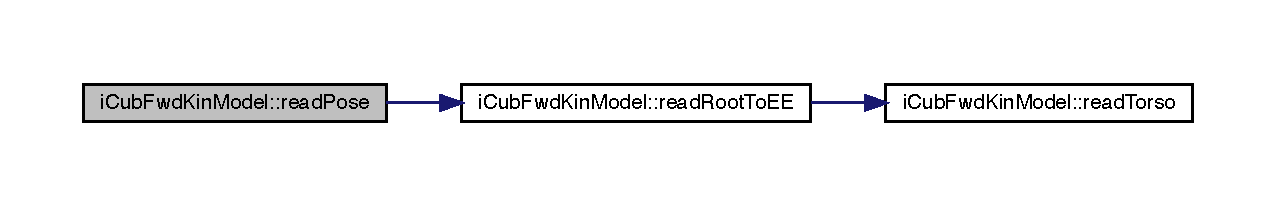
\includegraphics[width=350pt]{classiCubFwdKinModel_ad549519048e9b54c18af51c6b173b726_cgraph}
\end{center}
\end{figure}
\mbox{\Hypertarget{classiCubFwdKinModel_a638ea7ef68d98f306346684c93934a93}\label{classiCubFwdKinModel_a638ea7ef68d98f306346684c93934a93}} 
\index{i\+Cub\+Fwd\+Kin\+Model@{i\+Cub\+Fwd\+Kin\+Model}!read\+Root\+To\+EE@{read\+Root\+To\+EE}}
\index{read\+Root\+To\+EE@{read\+Root\+To\+EE}!i\+Cub\+Fwd\+Kin\+Model@{i\+Cub\+Fwd\+Kin\+Model}}
\subsubsection{\texorpdfstring{read\+Root\+To\+E\+E()}{readRootToEE()}}
{\footnotesize\ttfamily Vector i\+Cub\+Fwd\+Kin\+Model\+::read\+Root\+To\+EE (\begin{DoxyParamCaption}{ }\end{DoxyParamCaption})\hspace{0.3cm}{\ttfamily [protected]}}



Definition at line 133 of file i\+Cub\+Fwd\+Kin\+Model.\+cpp.



References itf\+\_\+arm\+\_\+enc\+\_\+, and read\+Torso().



Referenced by read\+Pose().

Here is the call graph for this function\+:
\nopagebreak
\begin{figure}[H]
\begin{center}
\leavevmode
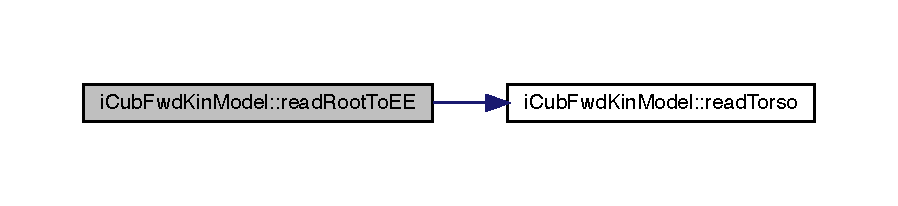
\includegraphics[width=350pt]{classiCubFwdKinModel_a638ea7ef68d98f306346684c93934a93_cgraph}
\end{center}
\end{figure}
\mbox{\Hypertarget{classiCubFwdKinModel_a4ed6df084a996223a740a7065e16b799}\label{classiCubFwdKinModel_a4ed6df084a996223a740a7065e16b799}} 
\index{i\+Cub\+Fwd\+Kin\+Model@{i\+Cub\+Fwd\+Kin\+Model}!read\+Torso@{read\+Torso}}
\index{read\+Torso@{read\+Torso}!i\+Cub\+Fwd\+Kin\+Model@{i\+Cub\+Fwd\+Kin\+Model}}
\subsubsection{\texorpdfstring{read\+Torso()}{readTorso()}}
{\footnotesize\ttfamily Vector i\+Cub\+Fwd\+Kin\+Model\+::read\+Torso (\begin{DoxyParamCaption}{ }\end{DoxyParamCaption})\hspace{0.3cm}{\ttfamily [protected]}}



Definition at line 119 of file i\+Cub\+Fwd\+Kin\+Model.\+cpp.



References itf\+\_\+torso\+\_\+enc\+\_\+.



Referenced by read\+Root\+To\+E\+E().

\mbox{\Hypertarget{classFwdKinModel_a12b54bd62ba5cf218973c600c66ba39e}\label{classFwdKinModel_a12b54bd62ba5cf218973c600c66ba39e}} 
\index{i\+Cub\+Fwd\+Kin\+Model@{i\+Cub\+Fwd\+Kin\+Model}!set\+Delta\+Motion@{set\+Delta\+Motion}}
\index{set\+Delta\+Motion@{set\+Delta\+Motion}!i\+Cub\+Fwd\+Kin\+Model@{i\+Cub\+Fwd\+Kin\+Model}}
\subsubsection{\texorpdfstring{set\+Delta\+Motion()}{setDeltaMotion()}}
{\footnotesize\ttfamily bool Fwd\+Kin\+Model\+::set\+Delta\+Motion (\begin{DoxyParamCaption}{ }\end{DoxyParamCaption})\hspace{0.3cm}{\ttfamily [protected]}, {\ttfamily [inherited]}}



Definition at line 71 of file Fwd\+Kin\+Model.\+cpp.

\mbox{\Hypertarget{classiCubFwdKinModel_a2daa3bb3b2c458200dc487ac00929260}\label{classiCubFwdKinModel_a2daa3bb3b2c458200dc487ac00929260}} 
\index{i\+Cub\+Fwd\+Kin\+Model@{i\+Cub\+Fwd\+Kin\+Model}!set\+Property@{set\+Property}}
\index{set\+Property@{set\+Property}!i\+Cub\+Fwd\+Kin\+Model@{i\+Cub\+Fwd\+Kin\+Model}}
\subsubsection{\texorpdfstring{set\+Property()}{setProperty()}}
{\footnotesize\ttfamily bool i\+Cub\+Fwd\+Kin\+Model\+::set\+Property (\begin{DoxyParamCaption}\item[{const std\+::string \&}]{property }\end{DoxyParamCaption})\hspace{0.3cm}{\ttfamily [override]}}



Definition at line 105 of file i\+Cub\+Fwd\+Kin\+Model.\+cpp.



References Fwd\+Kin\+Model\+::set\+Property().

Here is the call graph for this function\+:
\nopagebreak
\begin{figure}[H]
\begin{center}
\leavevmode
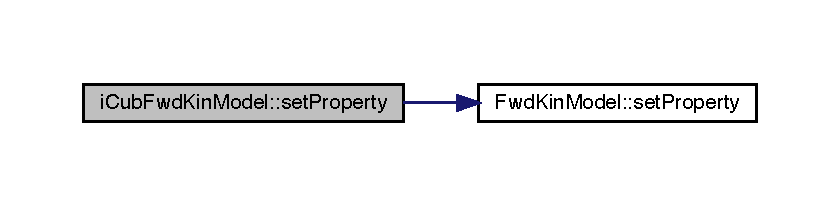
\includegraphics[width=350pt]{classiCubFwdKinModel_a2daa3bb3b2c458200dc487ac00929260_cgraph}
\end{center}
\end{figure}


\subsection{Member Data Documentation}
\mbox{\Hypertarget{classiCubFwdKinModel_a3a07f11e9b770e8fc7c03bff05c52927}\label{classiCubFwdKinModel_a3a07f11e9b770e8fc7c03bff05c52927}} 
\index{i\+Cub\+Fwd\+Kin\+Model@{i\+Cub\+Fwd\+Kin\+Model}!drv\+\_\+arm\+\_\+enc\+\_\+@{drv\+\_\+arm\+\_\+enc\+\_\+}}
\index{drv\+\_\+arm\+\_\+enc\+\_\+@{drv\+\_\+arm\+\_\+enc\+\_\+}!i\+Cub\+Fwd\+Kin\+Model@{i\+Cub\+Fwd\+Kin\+Model}}
\subsubsection{\texorpdfstring{drv\+\_\+arm\+\_\+enc\+\_\+}{drv\_arm\_enc\_}}
{\footnotesize\ttfamily yarp\+::dev\+::\+Poly\+Driver i\+Cub\+Fwd\+Kin\+Model\+::drv\+\_\+arm\+\_\+enc\+\_\+\hspace{0.3cm}{\ttfamily [protected]}}



Definition at line 29 of file i\+Cub\+Fwd\+Kin\+Model.\+h.



Referenced by i\+Cub\+Fwd\+Kin\+Model(), and $\sim$i\+Cub\+Fwd\+Kin\+Model().

\mbox{\Hypertarget{classiCubFwdKinModel_af0ca571291c508a2a058c1ff802e6421}\label{classiCubFwdKinModel_af0ca571291c508a2a058c1ff802e6421}} 
\index{i\+Cub\+Fwd\+Kin\+Model@{i\+Cub\+Fwd\+Kin\+Model}!drv\+\_\+torso\+\_\+enc\+\_\+@{drv\+\_\+torso\+\_\+enc\+\_\+}}
\index{drv\+\_\+torso\+\_\+enc\+\_\+@{drv\+\_\+torso\+\_\+enc\+\_\+}!i\+Cub\+Fwd\+Kin\+Model@{i\+Cub\+Fwd\+Kin\+Model}}
\subsubsection{\texorpdfstring{drv\+\_\+torso\+\_\+enc\+\_\+}{drv\_torso\_enc\_}}
{\footnotesize\ttfamily yarp\+::dev\+::\+Poly\+Driver i\+Cub\+Fwd\+Kin\+Model\+::drv\+\_\+torso\+\_\+enc\+\_\+\hspace{0.3cm}{\ttfamily [protected]}}



Definition at line 30 of file i\+Cub\+Fwd\+Kin\+Model.\+h.



Referenced by i\+Cub\+Fwd\+Kin\+Model(), and $\sim$i\+Cub\+Fwd\+Kin\+Model().

\mbox{\Hypertarget{classiCubFwdKinModel_a4b92808d2c83eaff8a3bf18dede7001a}\label{classiCubFwdKinModel_a4b92808d2c83eaff8a3bf18dede7001a}} 
\index{i\+Cub\+Fwd\+Kin\+Model@{i\+Cub\+Fwd\+Kin\+Model}!icub\+\_\+kin\+\_\+arm\+\_\+@{icub\+\_\+kin\+\_\+arm\+\_\+}}
\index{icub\+\_\+kin\+\_\+arm\+\_\+@{icub\+\_\+kin\+\_\+arm\+\_\+}!i\+Cub\+Fwd\+Kin\+Model@{i\+Cub\+Fwd\+Kin\+Model}}
\subsubsection{\texorpdfstring{icub\+\_\+kin\+\_\+arm\+\_\+}{icub\_kin\_arm\_}}
{\footnotesize\ttfamily i\+Cub\+::i\+Kin\+::i\+Cub\+Arm i\+Cub\+Fwd\+Kin\+Model\+::icub\+\_\+kin\+\_\+arm\+\_\+\hspace{0.3cm}{\ttfamily [protected]}}



Definition at line 33 of file i\+Cub\+Fwd\+Kin\+Model.\+h.



Referenced by i\+Cub\+Fwd\+Kin\+Model(), and read\+Pose().

\mbox{\Hypertarget{classiCubFwdKinModel_a3eb6c400ef775a5549aa31fe22fae4c0}\label{classiCubFwdKinModel_a3eb6c400ef775a5549aa31fe22fae4c0}} 
\index{i\+Cub\+Fwd\+Kin\+Model@{i\+Cub\+Fwd\+Kin\+Model}!I\+D\+\_\+@{I\+D\+\_\+}}
\index{I\+D\+\_\+@{I\+D\+\_\+}!i\+Cub\+Fwd\+Kin\+Model@{i\+Cub\+Fwd\+Kin\+Model}}
\subsubsection{\texorpdfstring{I\+D\+\_\+}{ID\_}}
{\footnotesize\ttfamily yarp\+::os\+::\+Const\+String i\+Cub\+Fwd\+Kin\+Model\+::\+I\+D\+\_\+ = \char`\"{}i\+Cub\+Fwd\+Kin\+Model\char`\"{}\hspace{0.3cm}{\ttfamily [private]}}



Definition at line 36 of file i\+Cub\+Fwd\+Kin\+Model.\+h.



Referenced by i\+Cub\+Fwd\+Kin\+Model().

\mbox{\Hypertarget{classFwdKinModel_a2ed7b77ebd710e5debe63b83a34a1645}\label{classFwdKinModel_a2ed7b77ebd710e5debe63b83a34a1645}} 
\index{i\+Cub\+Fwd\+Kin\+Model@{i\+Cub\+Fwd\+Kin\+Model}!initialize\+\_\+delta\+\_\+@{initialize\+\_\+delta\+\_\+}}
\index{initialize\+\_\+delta\+\_\+@{initialize\+\_\+delta\+\_\+}!i\+Cub\+Fwd\+Kin\+Model@{i\+Cub\+Fwd\+Kin\+Model}}
\subsubsection{\texorpdfstring{initialize\+\_\+delta\+\_\+}{initialize\_delta\_}}
{\footnotesize\ttfamily bool Fwd\+Kin\+Model\+::initialize\+\_\+delta\+\_\+ = true\hspace{0.3cm}{\ttfamily [protected]}, {\ttfamily [inherited]}}



Definition at line 28 of file Fwd\+Kin\+Model.\+h.

\mbox{\Hypertarget{classiCubFwdKinModel_a4478fa4b4f0689d819a19a5cccd69ae2}\label{classiCubFwdKinModel_a4478fa4b4f0689d819a19a5cccd69ae2}} 
\index{i\+Cub\+Fwd\+Kin\+Model@{i\+Cub\+Fwd\+Kin\+Model}!itf\+\_\+arm\+\_\+enc\+\_\+@{itf\+\_\+arm\+\_\+enc\+\_\+}}
\index{itf\+\_\+arm\+\_\+enc\+\_\+@{itf\+\_\+arm\+\_\+enc\+\_\+}!i\+Cub\+Fwd\+Kin\+Model@{i\+Cub\+Fwd\+Kin\+Model}}
\subsubsection{\texorpdfstring{itf\+\_\+arm\+\_\+enc\+\_\+}{itf\_arm\_enc\_}}
{\footnotesize\ttfamily yarp\+::dev\+::\+I\+Encoders$\ast$ i\+Cub\+Fwd\+Kin\+Model\+::itf\+\_\+arm\+\_\+enc\+\_\+\hspace{0.3cm}{\ttfamily [protected]}}



Definition at line 31 of file i\+Cub\+Fwd\+Kin\+Model.\+h.



Referenced by i\+Cub\+Fwd\+Kin\+Model(), and read\+Root\+To\+E\+E().

\mbox{\Hypertarget{classiCubFwdKinModel_a2d83dd73bf08f66563e9e33d2c26d16a}\label{classiCubFwdKinModel_a2d83dd73bf08f66563e9e33d2c26d16a}} 
\index{i\+Cub\+Fwd\+Kin\+Model@{i\+Cub\+Fwd\+Kin\+Model}!itf\+\_\+torso\+\_\+enc\+\_\+@{itf\+\_\+torso\+\_\+enc\+\_\+}}
\index{itf\+\_\+torso\+\_\+enc\+\_\+@{itf\+\_\+torso\+\_\+enc\+\_\+}!i\+Cub\+Fwd\+Kin\+Model@{i\+Cub\+Fwd\+Kin\+Model}}
\subsubsection{\texorpdfstring{itf\+\_\+torso\+\_\+enc\+\_\+}{itf\_torso\_enc\_}}
{\footnotesize\ttfamily yarp\+::dev\+::\+I\+Encoders$\ast$ i\+Cub\+Fwd\+Kin\+Model\+::itf\+\_\+torso\+\_\+enc\+\_\+\hspace{0.3cm}{\ttfamily [protected]}}



Definition at line 32 of file i\+Cub\+Fwd\+Kin\+Model.\+h.



Referenced by i\+Cub\+Fwd\+Kin\+Model(), and read\+Torso().

\mbox{\Hypertarget{classiCubFwdKinModel_a9894964cecb15d56a55ea1f4610a1cbe}\label{classiCubFwdKinModel_a9894964cecb15d56a55ea1f4610a1cbe}} 
\index{i\+Cub\+Fwd\+Kin\+Model@{i\+Cub\+Fwd\+Kin\+Model}!laterality\+\_\+@{laterality\+\_\+}}
\index{laterality\+\_\+@{laterality\+\_\+}!i\+Cub\+Fwd\+Kin\+Model@{i\+Cub\+Fwd\+Kin\+Model}}
\subsubsection{\texorpdfstring{laterality\+\_\+}{laterality\_}}
{\footnotesize\ttfamily yarp\+::os\+::\+Const\+String i\+Cub\+Fwd\+Kin\+Model\+::laterality\+\_\+\hspace{0.3cm}{\ttfamily [private]}}



Definition at line 40 of file i\+Cub\+Fwd\+Kin\+Model.\+h.



Referenced by i\+Cub\+Fwd\+Kin\+Model().

\mbox{\Hypertarget{classiCubFwdKinModel_a091abb2a5386537d63a67fbf761a2e8a}\label{classiCubFwdKinModel_a091abb2a5386537d63a67fbf761a2e8a}} 
\index{i\+Cub\+Fwd\+Kin\+Model@{i\+Cub\+Fwd\+Kin\+Model}!log\+\_\+\+I\+D\+\_\+@{log\+\_\+\+I\+D\+\_\+}}
\index{log\+\_\+\+I\+D\+\_\+@{log\+\_\+\+I\+D\+\_\+}!i\+Cub\+Fwd\+Kin\+Model@{i\+Cub\+Fwd\+Kin\+Model}}
\subsubsection{\texorpdfstring{log\+\_\+\+I\+D\+\_\+}{log\_ID\_}}
{\footnotesize\ttfamily yarp\+::os\+::\+Const\+String i\+Cub\+Fwd\+Kin\+Model\+::log\+\_\+\+I\+D\+\_\+ = \char`\"{}\mbox{[}\char`\"{} + \hyperlink{classiCubFwdKinModel_a3eb6c400ef775a5549aa31fe22fae4c0}{I\+D\+\_\+} + \char`\"{}\mbox{]}\char`\"{}\hspace{0.3cm}{\ttfamily [private]}}



Definition at line 37 of file i\+Cub\+Fwd\+Kin\+Model.\+h.



Referenced by i\+Cub\+Fwd\+Kin\+Model().

\mbox{\Hypertarget{classiCubFwdKinModel_a294f61787264b6a3e9dc1eb9dbc72ed0}\label{classiCubFwdKinModel_a294f61787264b6a3e9dc1eb9dbc72ed0}} 
\index{i\+Cub\+Fwd\+Kin\+Model@{i\+Cub\+Fwd\+Kin\+Model}!port\+\_\+prefix\+\_\+@{port\+\_\+prefix\+\_\+}}
\index{port\+\_\+prefix\+\_\+@{port\+\_\+prefix\+\_\+}!i\+Cub\+Fwd\+Kin\+Model@{i\+Cub\+Fwd\+Kin\+Model}}
\subsubsection{\texorpdfstring{port\+\_\+prefix\+\_\+}{port\_prefix\_}}
{\footnotesize\ttfamily yarp\+::os\+::\+Const\+String i\+Cub\+Fwd\+Kin\+Model\+::port\+\_\+prefix\+\_\+\hspace{0.3cm}{\ttfamily [private]}}



Definition at line 41 of file i\+Cub\+Fwd\+Kin\+Model.\+h.

\mbox{\Hypertarget{classiCubFwdKinModel_ad0fec4635ff934435b24d717cb553014}\label{classiCubFwdKinModel_ad0fec4635ff934435b24d717cb553014}} 
\index{i\+Cub\+Fwd\+Kin\+Model@{i\+Cub\+Fwd\+Kin\+Model}!robot\+\_\+@{robot\+\_\+}}
\index{robot\+\_\+@{robot\+\_\+}!i\+Cub\+Fwd\+Kin\+Model@{i\+Cub\+Fwd\+Kin\+Model}}
\subsubsection{\texorpdfstring{robot\+\_\+}{robot\_}}
{\footnotesize\ttfamily yarp\+::os\+::\+Const\+String i\+Cub\+Fwd\+Kin\+Model\+::robot\+\_\+\hspace{0.3cm}{\ttfamily [private]}}



Definition at line 39 of file i\+Cub\+Fwd\+Kin\+Model.\+h.



Referenced by i\+Cub\+Fwd\+Kin\+Model().



The documentation for this class was generated from the following files\+:\begin{DoxyCompactItemize}
\item 
/\+Users/\+Claudio/\+Git\+Hub/visual-\/tracking-\/control/src/hand-\/tracking/include/\hyperlink{iCubFwdKinModel_8h}{i\+Cub\+Fwd\+Kin\+Model.\+h}\item 
/\+Users/\+Claudio/\+Git\+Hub/visual-\/tracking-\/control/src/hand-\/tracking/src/\hyperlink{iCubFwdKinModel_8cpp}{i\+Cub\+Fwd\+Kin\+Model.\+cpp}\end{DoxyCompactItemize}

\hypertarget{classiCubGatePose}{}\section{i\+Cub\+Gate\+Pose Class Reference}
\label{classiCubGatePose}\index{i\+Cub\+Gate\+Pose@{i\+Cub\+Gate\+Pose}}


{\ttfamily \#include $<$i\+Cub\+Gate\+Pose.\+h$>$}



Inheritance diagram for i\+Cub\+Gate\+Pose\+:
\nopagebreak
\begin{figure}[H]
\begin{center}
\leavevmode
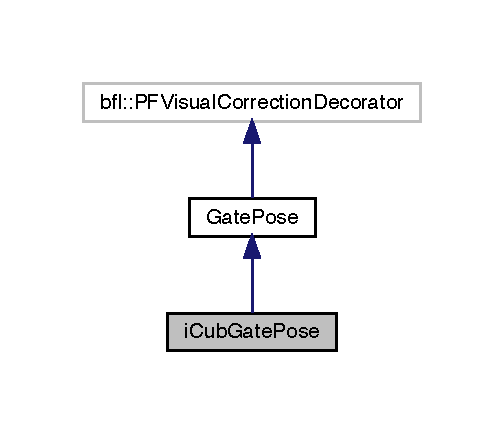
\includegraphics[width=242pt]{classiCubGatePose__inherit__graph}
\end{center}
\end{figure}
\subsection*{Public Member Functions}
\begin{DoxyCompactItemize}
\item 
\hyperlink{classiCubGatePose_a3c06ef47eb5a0ccb0500828829fa3c31}{i\+Cub\+Gate\+Pose} (std\+::unique\+\_\+ptr$<$ P\+F\+Visual\+Correction $>$ visual\+\_\+correction, const double gate\+\_\+x, const double gate\+\_\+y, const double gate\+\_\+z, const double gate\+\_\+aperture, const double gate\+\_\+rotation, const yarp\+::os\+::\+Const\+String \&robot, const yarp\+::os\+::\+Const\+String \&laterality, const yarp\+::os\+::\+Const\+String \&port\+\_\+prefix)
\item 
\hyperlink{classiCubGatePose_a6b852c2c3b8c542b33d6b5e129f2ef54}{i\+Cub\+Gate\+Pose} (std\+::unique\+\_\+ptr$<$ P\+F\+Visual\+Correction $>$ visual\+\_\+correction, const yarp\+::os\+::\+Const\+String \&robot, const yarp\+::os\+::\+Const\+String \&laterality, const yarp\+::os\+::\+Const\+String \&port\+\_\+prefix)
\item 
\hyperlink{classiCubGatePose_a4c1d13f972ab4b9c778982964dae768d}{$\sim$i\+Cub\+Gate\+Pose} () noexcept override
\item 
void \hyperlink{classGatePose_a00607a4325dcfb7a02bda7490b65d25c}{innovation} (const Eigen\+::\+Ref$<$ const Eigen\+::\+Matrix\+Xf $>$ \&pred\+\_\+states, cv\+::\+Input\+Array measurements, Eigen\+::\+Ref$<$ Eigen\+::\+Matrix\+Xf $>$ innovations) override
\item 
double \hyperlink{classGatePose_a939c575d5d59c8b0f3ab528edd368c0d}{likelihood} (const Eigen\+::\+Ref$<$ const Eigen\+::\+Matrix\+Xf $>$ \&innovations) override
\item 
bfl\+::\+Visual\+Observation\+Model \& \hyperlink{classGatePose_aa47f9242f039b8752675db5594350a28}{get\+Visual\+Observation\+Model} () override
\item 
void \hyperlink{classGatePose_a18ba358c801ae1a246dbee2f9780c698}{set\+Visual\+Observation\+Model} (std\+::unique\+\_\+ptr$<$ bfl\+::\+Visual\+Observation\+Model $>$ visual\+\_\+observation\+\_\+model) override
\end{DoxyCompactItemize}
\subsection*{Protected Member Functions}
\begin{DoxyCompactItemize}
\item 
Eigen\+::\+Vector\+Xd \hyperlink{classiCubGatePose_aff1494edcf8f17803788f954ba0b443b}{read\+Pose} () override
\item 
yarp\+::sig\+::\+Vector \hyperlink{classiCubGatePose_a78b89d0b90d60b37a5f613718d384590}{read\+Root\+To\+EE} ()
\item 
yarp\+::sig\+::\+Vector \hyperlink{classiCubGatePose_ab03607afcf2246d5d1d18835c623fc34}{read\+Torso} ()
\item 
void \hyperlink{classGatePose_a91d395abe75dc7772116f50219dc19ae}{correct\+Step} (const Eigen\+::\+Ref$<$ const Eigen\+::\+Matrix\+Xf $>$ \&pred\+\_\+states, const Eigen\+::\+Ref$<$ const Eigen\+::\+Vector\+Xf $>$ \&pred\+\_\+weights, cv\+::\+Input\+Array measurements, Eigen\+::\+Ref$<$ Eigen\+::\+Matrix\+Xf $>$ cor\+\_\+states, Eigen\+::\+Ref$<$ Eigen\+::\+Vector\+Xf $>$ cor\+\_\+weights) override
\item 
bool \hyperlink{classGatePose_a880273787b1b3542e1e7971954ac118d}{is\+Inside\+Ellipsoid} (const Eigen\+::\+Ref$<$ const Eigen\+::\+Vector\+Xf $>$ \&state)
\item 
bool \hyperlink{classGatePose_a6d188756ed5dcc56c311a2aafc9d1acd}{is\+Within\+Rotation} (float rot\+\_\+angle)
\item 
bool \hyperlink{classGatePose_ad2e8708b3ed5a8252bdec1494f199fda}{is\+Inside\+Cone} (const Eigen\+::\+Ref$<$ const Eigen\+::\+Vector\+Xf $>$ \&state)
\end{DoxyCompactItemize}
\subsection*{Protected Attributes}
\begin{DoxyCompactItemize}
\item 
yarp\+::dev\+::\+Poly\+Driver \hyperlink{classiCubGatePose_ab365d41c45121ee8ec048506f952d252}{drv\+\_\+arm\+\_\+enc\+\_\+}
\item 
yarp\+::dev\+::\+I\+Encoders $\ast$ \hyperlink{classiCubGatePose_ad953e2818c3927e941404522bddf98cb}{itf\+\_\+arm\+\_\+enc\+\_\+}
\item 
yarp\+::dev\+::\+Poly\+Driver \hyperlink{classiCubGatePose_a165a41ce9ec94e024f2aabcfb911ef0b}{drv\+\_\+torso\+\_\+enc\+\_\+}
\item 
yarp\+::dev\+::\+I\+Encoders $\ast$ \hyperlink{classiCubGatePose_abc096becfdfdc97811ed8cfdc13e282c}{itf\+\_\+torso\+\_\+enc\+\_\+}
\item 
i\+Cub\+::i\+Kin\+::i\+Cub\+Arm \hyperlink{classiCubGatePose_aa456e07e3cdbfd4bc1bdf0ed1b56f551}{icub\+\_\+kin\+\_\+arm\+\_\+}
\end{DoxyCompactItemize}
\subsection*{Private Attributes}
\begin{DoxyCompactItemize}
\item 
const yarp\+::os\+::\+Const\+String \hyperlink{classiCubGatePose_a2e70b20ff45c269bfb6a339792f51fd0}{I\+D\+\_\+} = \char`\"{}i\+Cub\+Gate\+Pose\char`\"{}
\item 
const yarp\+::os\+::\+Const\+String \hyperlink{classiCubGatePose_a79abca8331a8c99fcf05e44e681fe067}{log\+\_\+\+I\+D\+\_\+} = \char`\"{}\mbox{[}\char`\"{} + \hyperlink{classiCubGatePose_a2e70b20ff45c269bfb6a339792f51fd0}{I\+D\+\_\+} + \char`\"{}\mbox{]}\char`\"{}
\item 
yarp\+::os\+::\+Const\+String \hyperlink{classiCubGatePose_a15e5113dc88ac3b411eaa33d60378b66}{robot\+\_\+}
\item 
yarp\+::os\+::\+Const\+String \hyperlink{classiCubGatePose_a738def17b96e37617d7a7ca9365bae6d}{laterality\+\_\+}
\item 
yarp\+::os\+::\+Const\+String \hyperlink{classiCubGatePose_a2e319d826c8683417b96d691f9d5fa58}{port\+\_\+prefix\+\_\+}
\end{DoxyCompactItemize}


\subsection{Detailed Description}


Definition at line 13 of file i\+Cub\+Gate\+Pose.\+h.



\subsection{Constructor \& Destructor Documentation}
\mbox{\Hypertarget{classiCubGatePose_a3c06ef47eb5a0ccb0500828829fa3c31}\label{classiCubGatePose_a3c06ef47eb5a0ccb0500828829fa3c31}} 
\index{i\+Cub\+Gate\+Pose@{i\+Cub\+Gate\+Pose}!i\+Cub\+Gate\+Pose@{i\+Cub\+Gate\+Pose}}
\index{i\+Cub\+Gate\+Pose@{i\+Cub\+Gate\+Pose}!i\+Cub\+Gate\+Pose@{i\+Cub\+Gate\+Pose}}
\subsubsection{\texorpdfstring{i\+Cub\+Gate\+Pose()}{iCubGatePose()}\hspace{0.1cm}{\footnotesize\ttfamily [1/2]}}
{\footnotesize\ttfamily i\+Cub\+Gate\+Pose\+::i\+Cub\+Gate\+Pose (\begin{DoxyParamCaption}\item[{std\+::unique\+\_\+ptr$<$ P\+F\+Visual\+Correction $>$}]{visual\+\_\+correction,  }\item[{const double}]{gate\+\_\+x,  }\item[{const double}]{gate\+\_\+y,  }\item[{const double}]{gate\+\_\+z,  }\item[{const double}]{gate\+\_\+aperture,  }\item[{const double}]{gate\+\_\+rotation,  }\item[{const yarp\+::os\+::\+Const\+String \&}]{robot,  }\item[{const yarp\+::os\+::\+Const\+String \&}]{laterality,  }\item[{const yarp\+::os\+::\+Const\+String \&}]{port\+\_\+prefix }\end{DoxyParamCaption})}



Definition at line 19 of file i\+Cub\+Gate\+Pose.\+cpp.



References drv\+\_\+arm\+\_\+enc\+\_\+, drv\+\_\+torso\+\_\+enc\+\_\+, icub\+\_\+kin\+\_\+arm\+\_\+, I\+D\+\_\+, itf\+\_\+arm\+\_\+enc\+\_\+, itf\+\_\+torso\+\_\+enc\+\_\+, laterality\+\_\+, log\+\_\+\+I\+D\+\_\+, and robot\+\_\+.

\mbox{\Hypertarget{classiCubGatePose_a6b852c2c3b8c542b33d6b5e129f2ef54}\label{classiCubGatePose_a6b852c2c3b8c542b33d6b5e129f2ef54}} 
\index{i\+Cub\+Gate\+Pose@{i\+Cub\+Gate\+Pose}!i\+Cub\+Gate\+Pose@{i\+Cub\+Gate\+Pose}}
\index{i\+Cub\+Gate\+Pose@{i\+Cub\+Gate\+Pose}!i\+Cub\+Gate\+Pose@{i\+Cub\+Gate\+Pose}}
\subsubsection{\texorpdfstring{i\+Cub\+Gate\+Pose()}{iCubGatePose()}\hspace{0.1cm}{\footnotesize\ttfamily [2/2]}}
{\footnotesize\ttfamily i\+Cub\+Gate\+Pose\+::i\+Cub\+Gate\+Pose (\begin{DoxyParamCaption}\item[{std\+::unique\+\_\+ptr$<$ P\+F\+Visual\+Correction $>$}]{visual\+\_\+correction,  }\item[{const yarp\+::os\+::\+Const\+String \&}]{robot,  }\item[{const yarp\+::os\+::\+Const\+String \&}]{laterality,  }\item[{const yarp\+::os\+::\+Const\+String \&}]{port\+\_\+prefix }\end{DoxyParamCaption})}



Definition at line 102 of file i\+Cub\+Gate\+Pose.\+cpp.

\mbox{\Hypertarget{classiCubGatePose_a4c1d13f972ab4b9c778982964dae768d}\label{classiCubGatePose_a4c1d13f972ab4b9c778982964dae768d}} 
\index{i\+Cub\+Gate\+Pose@{i\+Cub\+Gate\+Pose}!````~i\+Cub\+Gate\+Pose@{$\sim$i\+Cub\+Gate\+Pose}}
\index{````~i\+Cub\+Gate\+Pose@{$\sim$i\+Cub\+Gate\+Pose}!i\+Cub\+Gate\+Pose@{i\+Cub\+Gate\+Pose}}
\subsubsection{\texorpdfstring{$\sim$i\+Cub\+Gate\+Pose()}{~iCubGatePose()}}
{\footnotesize\ttfamily i\+Cub\+Gate\+Pose\+::$\sim$i\+Cub\+Gate\+Pose (\begin{DoxyParamCaption}{ }\end{DoxyParamCaption})\hspace{0.3cm}{\ttfamily [override]}, {\ttfamily [noexcept]}}



Definition at line 107 of file i\+Cub\+Gate\+Pose.\+cpp.



\subsection{Member Function Documentation}
\mbox{\Hypertarget{classGatePose_a91d395abe75dc7772116f50219dc19ae}\label{classGatePose_a91d395abe75dc7772116f50219dc19ae}} 
\index{i\+Cub\+Gate\+Pose@{i\+Cub\+Gate\+Pose}!correct\+Step@{correct\+Step}}
\index{correct\+Step@{correct\+Step}!i\+Cub\+Gate\+Pose@{i\+Cub\+Gate\+Pose}}
\subsubsection{\texorpdfstring{correct\+Step()}{correctStep()}}
{\footnotesize\ttfamily void Gate\+Pose\+::correct\+Step (\begin{DoxyParamCaption}\item[{const Eigen\+::\+Ref$<$ const Eigen\+::\+Matrix\+Xf $>$ \&}]{pred\+\_\+states,  }\item[{const Eigen\+::\+Ref$<$ const Eigen\+::\+Vector\+Xf $>$ \&}]{pred\+\_\+weights,  }\item[{cv\+::\+Input\+Array}]{measurements,  }\item[{Eigen\+::\+Ref$<$ Eigen\+::\+Matrix\+Xf $>$}]{cor\+\_\+states,  }\item[{Eigen\+::\+Ref$<$ Eigen\+::\+Vector\+Xf $>$}]{cor\+\_\+weights }\end{DoxyParamCaption})\hspace{0.3cm}{\ttfamily [override]}, {\ttfamily [protected]}, {\ttfamily [inherited]}}



Definition at line 54 of file Gate\+Pose.\+cpp.

\mbox{\Hypertarget{classGatePose_aa47f9242f039b8752675db5594350a28}\label{classGatePose_aa47f9242f039b8752675db5594350a28}} 
\index{i\+Cub\+Gate\+Pose@{i\+Cub\+Gate\+Pose}!get\+Visual\+Observation\+Model@{get\+Visual\+Observation\+Model}}
\index{get\+Visual\+Observation\+Model@{get\+Visual\+Observation\+Model}!i\+Cub\+Gate\+Pose@{i\+Cub\+Gate\+Pose}}
\subsubsection{\texorpdfstring{get\+Visual\+Observation\+Model()}{getVisualObservationModel()}}
{\footnotesize\ttfamily Visual\+Observation\+Model \& Gate\+Pose\+::get\+Visual\+Observation\+Model (\begin{DoxyParamCaption}{ }\end{DoxyParamCaption})\hspace{0.3cm}{\ttfamily [override]}, {\ttfamily [inherited]}}



Definition at line 42 of file Gate\+Pose.\+cpp.

\mbox{\Hypertarget{classGatePose_a00607a4325dcfb7a02bda7490b65d25c}\label{classGatePose_a00607a4325dcfb7a02bda7490b65d25c}} 
\index{i\+Cub\+Gate\+Pose@{i\+Cub\+Gate\+Pose}!innovation@{innovation}}
\index{innovation@{innovation}!i\+Cub\+Gate\+Pose@{i\+Cub\+Gate\+Pose}}
\subsubsection{\texorpdfstring{innovation()}{innovation()}}
{\footnotesize\ttfamily void Gate\+Pose\+::innovation (\begin{DoxyParamCaption}\item[{const Eigen\+::\+Ref$<$ const Eigen\+::\+Matrix\+Xf $>$ \&}]{pred\+\_\+states,  }\item[{cv\+::\+Input\+Array}]{measurements,  }\item[{Eigen\+::\+Ref$<$ Eigen\+::\+Matrix\+Xf $>$}]{innovations }\end{DoxyParamCaption})\hspace{0.3cm}{\ttfamily [override]}, {\ttfamily [inherited]}}



Definition at line 30 of file Gate\+Pose.\+cpp.

\mbox{\Hypertarget{classGatePose_ad2e8708b3ed5a8252bdec1494f199fda}\label{classGatePose_ad2e8708b3ed5a8252bdec1494f199fda}} 
\index{i\+Cub\+Gate\+Pose@{i\+Cub\+Gate\+Pose}!is\+Inside\+Cone@{is\+Inside\+Cone}}
\index{is\+Inside\+Cone@{is\+Inside\+Cone}!i\+Cub\+Gate\+Pose@{i\+Cub\+Gate\+Pose}}
\subsubsection{\texorpdfstring{is\+Inside\+Cone()}{isInsideCone()}}
{\footnotesize\ttfamily bool Gate\+Pose\+::is\+Inside\+Cone (\begin{DoxyParamCaption}\item[{const Eigen\+::\+Ref$<$ const Eigen\+::\+Vector\+Xf $>$ \&}]{state }\end{DoxyParamCaption})\hspace{0.3cm}{\ttfamily [protected]}, {\ttfamily [inherited]}}



Definition at line 88 of file Gate\+Pose.\+cpp.

\mbox{\Hypertarget{classGatePose_a880273787b1b3542e1e7971954ac118d}\label{classGatePose_a880273787b1b3542e1e7971954ac118d}} 
\index{i\+Cub\+Gate\+Pose@{i\+Cub\+Gate\+Pose}!is\+Inside\+Ellipsoid@{is\+Inside\+Ellipsoid}}
\index{is\+Inside\+Ellipsoid@{is\+Inside\+Ellipsoid}!i\+Cub\+Gate\+Pose@{i\+Cub\+Gate\+Pose}}
\subsubsection{\texorpdfstring{is\+Inside\+Ellipsoid()}{isInsideEllipsoid()}}
{\footnotesize\ttfamily bool Gate\+Pose\+::is\+Inside\+Ellipsoid (\begin{DoxyParamCaption}\item[{const Eigen\+::\+Ref$<$ const Eigen\+::\+Vector\+Xf $>$ \&}]{state }\end{DoxyParamCaption})\hspace{0.3cm}{\ttfamily [protected]}, {\ttfamily [inherited]}}



Definition at line 72 of file Gate\+Pose.\+cpp.

\mbox{\Hypertarget{classGatePose_a6d188756ed5dcc56c311a2aafc9d1acd}\label{classGatePose_a6d188756ed5dcc56c311a2aafc9d1acd}} 
\index{i\+Cub\+Gate\+Pose@{i\+Cub\+Gate\+Pose}!is\+Within\+Rotation@{is\+Within\+Rotation}}
\index{is\+Within\+Rotation@{is\+Within\+Rotation}!i\+Cub\+Gate\+Pose@{i\+Cub\+Gate\+Pose}}
\subsubsection{\texorpdfstring{is\+Within\+Rotation()}{isWithinRotation()}}
{\footnotesize\ttfamily bool Gate\+Pose\+::is\+Within\+Rotation (\begin{DoxyParamCaption}\item[{float}]{rot\+\_\+angle }\end{DoxyParamCaption})\hspace{0.3cm}{\ttfamily [protected]}, {\ttfamily [inherited]}}



Definition at line 80 of file Gate\+Pose.\+cpp.

\mbox{\Hypertarget{classGatePose_a939c575d5d59c8b0f3ab528edd368c0d}\label{classGatePose_a939c575d5d59c8b0f3ab528edd368c0d}} 
\index{i\+Cub\+Gate\+Pose@{i\+Cub\+Gate\+Pose}!likelihood@{likelihood}}
\index{likelihood@{likelihood}!i\+Cub\+Gate\+Pose@{i\+Cub\+Gate\+Pose}}
\subsubsection{\texorpdfstring{likelihood()}{likelihood()}}
{\footnotesize\ttfamily double Gate\+Pose\+::likelihood (\begin{DoxyParamCaption}\item[{const Eigen\+::\+Ref$<$ const Eigen\+::\+Matrix\+Xf $>$ \&}]{innovations }\end{DoxyParamCaption})\hspace{0.3cm}{\ttfamily [override]}, {\ttfamily [inherited]}}



Definition at line 36 of file Gate\+Pose.\+cpp.

\mbox{\Hypertarget{classiCubGatePose_aff1494edcf8f17803788f954ba0b443b}\label{classiCubGatePose_aff1494edcf8f17803788f954ba0b443b}} 
\index{i\+Cub\+Gate\+Pose@{i\+Cub\+Gate\+Pose}!read\+Pose@{read\+Pose}}
\index{read\+Pose@{read\+Pose}!i\+Cub\+Gate\+Pose@{i\+Cub\+Gate\+Pose}}
\subsubsection{\texorpdfstring{read\+Pose()}{readPose()}}
{\footnotesize\ttfamily Vector\+Xd i\+Cub\+Gate\+Pose\+::read\+Pose (\begin{DoxyParamCaption}{ }\end{DoxyParamCaption})\hspace{0.3cm}{\ttfamily [override]}, {\ttfamily [protected]}, {\ttfamily [virtual]}}



Implements \hyperlink{classGatePose_aed9235df850c3ca930f9e43276bf4f62}{Gate\+Pose}.



Definition at line 143 of file i\+Cub\+Gate\+Pose.\+cpp.



References icub\+\_\+kin\+\_\+arm\+\_\+, and read\+Root\+To\+E\+E().

Here is the call graph for this function\+:
\nopagebreak
\begin{figure}[H]
\begin{center}
\leavevmode
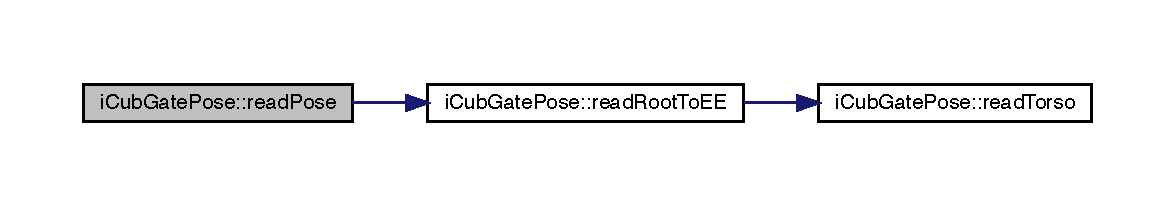
\includegraphics[width=350pt]{classiCubGatePose_aff1494edcf8f17803788f954ba0b443b_cgraph}
\end{center}
\end{figure}
\mbox{\Hypertarget{classiCubGatePose_a78b89d0b90d60b37a5f613718d384590}\label{classiCubGatePose_a78b89d0b90d60b37a5f613718d384590}} 
\index{i\+Cub\+Gate\+Pose@{i\+Cub\+Gate\+Pose}!read\+Root\+To\+EE@{read\+Root\+To\+EE}}
\index{read\+Root\+To\+EE@{read\+Root\+To\+EE}!i\+Cub\+Gate\+Pose@{i\+Cub\+Gate\+Pose}}
\subsubsection{\texorpdfstring{read\+Root\+To\+E\+E()}{readRootToEE()}}
{\footnotesize\ttfamily Vector i\+Cub\+Gate\+Pose\+::read\+Root\+To\+EE (\begin{DoxyParamCaption}{ }\end{DoxyParamCaption})\hspace{0.3cm}{\ttfamily [protected]}}



Definition at line 124 of file i\+Cub\+Gate\+Pose.\+cpp.



References itf\+\_\+arm\+\_\+enc\+\_\+, and read\+Torso().



Referenced by read\+Pose().

Here is the call graph for this function\+:
\nopagebreak
\begin{figure}[H]
\begin{center}
\leavevmode
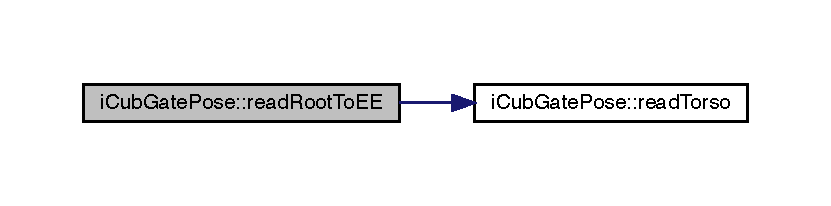
\includegraphics[width=350pt]{classiCubGatePose_a78b89d0b90d60b37a5f613718d384590_cgraph}
\end{center}
\end{figure}
\mbox{\Hypertarget{classiCubGatePose_ab03607afcf2246d5d1d18835c623fc34}\label{classiCubGatePose_ab03607afcf2246d5d1d18835c623fc34}} 
\index{i\+Cub\+Gate\+Pose@{i\+Cub\+Gate\+Pose}!read\+Torso@{read\+Torso}}
\index{read\+Torso@{read\+Torso}!i\+Cub\+Gate\+Pose@{i\+Cub\+Gate\+Pose}}
\subsubsection{\texorpdfstring{read\+Torso()}{readTorso()}}
{\footnotesize\ttfamily Vector i\+Cub\+Gate\+Pose\+::read\+Torso (\begin{DoxyParamCaption}{ }\end{DoxyParamCaption})\hspace{0.3cm}{\ttfamily [protected]}}



Definition at line 110 of file i\+Cub\+Gate\+Pose.\+cpp.



References itf\+\_\+torso\+\_\+enc\+\_\+.



Referenced by read\+Root\+To\+E\+E().

\mbox{\Hypertarget{classGatePose_a18ba358c801ae1a246dbee2f9780c698}\label{classGatePose_a18ba358c801ae1a246dbee2f9780c698}} 
\index{i\+Cub\+Gate\+Pose@{i\+Cub\+Gate\+Pose}!set\+Visual\+Observation\+Model@{set\+Visual\+Observation\+Model}}
\index{set\+Visual\+Observation\+Model@{set\+Visual\+Observation\+Model}!i\+Cub\+Gate\+Pose@{i\+Cub\+Gate\+Pose}}
\subsubsection{\texorpdfstring{set\+Visual\+Observation\+Model()}{setVisualObservationModel()}}
{\footnotesize\ttfamily void Gate\+Pose\+::set\+Visual\+Observation\+Model (\begin{DoxyParamCaption}\item[{std\+::unique\+\_\+ptr$<$ bfl\+::\+Visual\+Observation\+Model $>$}]{visual\+\_\+observation\+\_\+model }\end{DoxyParamCaption})\hspace{0.3cm}{\ttfamily [override]}, {\ttfamily [inherited]}}



Definition at line 48 of file Gate\+Pose.\+cpp.



\subsection{Member Data Documentation}
\mbox{\Hypertarget{classiCubGatePose_ab365d41c45121ee8ec048506f952d252}\label{classiCubGatePose_ab365d41c45121ee8ec048506f952d252}} 
\index{i\+Cub\+Gate\+Pose@{i\+Cub\+Gate\+Pose}!drv\+\_\+arm\+\_\+enc\+\_\+@{drv\+\_\+arm\+\_\+enc\+\_\+}}
\index{drv\+\_\+arm\+\_\+enc\+\_\+@{drv\+\_\+arm\+\_\+enc\+\_\+}!i\+Cub\+Gate\+Pose@{i\+Cub\+Gate\+Pose}}
\subsubsection{\texorpdfstring{drv\+\_\+arm\+\_\+enc\+\_\+}{drv\_arm\_enc\_}}
{\footnotesize\ttfamily yarp\+::dev\+::\+Poly\+Driver i\+Cub\+Gate\+Pose\+::drv\+\_\+arm\+\_\+enc\+\_\+\hspace{0.3cm}{\ttfamily [protected]}}



Definition at line 28 of file i\+Cub\+Gate\+Pose.\+h.



Referenced by i\+Cub\+Gate\+Pose().

\mbox{\Hypertarget{classiCubGatePose_a165a41ce9ec94e024f2aabcfb911ef0b}\label{classiCubGatePose_a165a41ce9ec94e024f2aabcfb911ef0b}} 
\index{i\+Cub\+Gate\+Pose@{i\+Cub\+Gate\+Pose}!drv\+\_\+torso\+\_\+enc\+\_\+@{drv\+\_\+torso\+\_\+enc\+\_\+}}
\index{drv\+\_\+torso\+\_\+enc\+\_\+@{drv\+\_\+torso\+\_\+enc\+\_\+}!i\+Cub\+Gate\+Pose@{i\+Cub\+Gate\+Pose}}
\subsubsection{\texorpdfstring{drv\+\_\+torso\+\_\+enc\+\_\+}{drv\_torso\_enc\_}}
{\footnotesize\ttfamily yarp\+::dev\+::\+Poly\+Driver i\+Cub\+Gate\+Pose\+::drv\+\_\+torso\+\_\+enc\+\_\+\hspace{0.3cm}{\ttfamily [protected]}}



Definition at line 30 of file i\+Cub\+Gate\+Pose.\+h.



Referenced by i\+Cub\+Gate\+Pose().

\mbox{\Hypertarget{classiCubGatePose_aa456e07e3cdbfd4bc1bdf0ed1b56f551}\label{classiCubGatePose_aa456e07e3cdbfd4bc1bdf0ed1b56f551}} 
\index{i\+Cub\+Gate\+Pose@{i\+Cub\+Gate\+Pose}!icub\+\_\+kin\+\_\+arm\+\_\+@{icub\+\_\+kin\+\_\+arm\+\_\+}}
\index{icub\+\_\+kin\+\_\+arm\+\_\+@{icub\+\_\+kin\+\_\+arm\+\_\+}!i\+Cub\+Gate\+Pose@{i\+Cub\+Gate\+Pose}}
\subsubsection{\texorpdfstring{icub\+\_\+kin\+\_\+arm\+\_\+}{icub\_kin\_arm\_}}
{\footnotesize\ttfamily i\+Cub\+::i\+Kin\+::i\+Cub\+Arm i\+Cub\+Gate\+Pose\+::icub\+\_\+kin\+\_\+arm\+\_\+\hspace{0.3cm}{\ttfamily [protected]}}



Definition at line 33 of file i\+Cub\+Gate\+Pose.\+h.



Referenced by i\+Cub\+Gate\+Pose(), and read\+Pose().

\mbox{\Hypertarget{classiCubGatePose_a2e70b20ff45c269bfb6a339792f51fd0}\label{classiCubGatePose_a2e70b20ff45c269bfb6a339792f51fd0}} 
\index{i\+Cub\+Gate\+Pose@{i\+Cub\+Gate\+Pose}!I\+D\+\_\+@{I\+D\+\_\+}}
\index{I\+D\+\_\+@{I\+D\+\_\+}!i\+Cub\+Gate\+Pose@{i\+Cub\+Gate\+Pose}}
\subsubsection{\texorpdfstring{I\+D\+\_\+}{ID\_}}
{\footnotesize\ttfamily const yarp\+::os\+::\+Const\+String i\+Cub\+Gate\+Pose\+::\+I\+D\+\_\+ = \char`\"{}i\+Cub\+Gate\+Pose\char`\"{}\hspace{0.3cm}{\ttfamily [private]}}



Definition at line 42 of file i\+Cub\+Gate\+Pose.\+h.



Referenced by i\+Cub\+Gate\+Pose().

\mbox{\Hypertarget{classiCubGatePose_ad953e2818c3927e941404522bddf98cb}\label{classiCubGatePose_ad953e2818c3927e941404522bddf98cb}} 
\index{i\+Cub\+Gate\+Pose@{i\+Cub\+Gate\+Pose}!itf\+\_\+arm\+\_\+enc\+\_\+@{itf\+\_\+arm\+\_\+enc\+\_\+}}
\index{itf\+\_\+arm\+\_\+enc\+\_\+@{itf\+\_\+arm\+\_\+enc\+\_\+}!i\+Cub\+Gate\+Pose@{i\+Cub\+Gate\+Pose}}
\subsubsection{\texorpdfstring{itf\+\_\+arm\+\_\+enc\+\_\+}{itf\_arm\_enc\_}}
{\footnotesize\ttfamily yarp\+::dev\+::\+I\+Encoders$\ast$ i\+Cub\+Gate\+Pose\+::itf\+\_\+arm\+\_\+enc\+\_\+\hspace{0.3cm}{\ttfamily [protected]}}



Definition at line 29 of file i\+Cub\+Gate\+Pose.\+h.



Referenced by i\+Cub\+Gate\+Pose(), and read\+Root\+To\+E\+E().

\mbox{\Hypertarget{classiCubGatePose_abc096becfdfdc97811ed8cfdc13e282c}\label{classiCubGatePose_abc096becfdfdc97811ed8cfdc13e282c}} 
\index{i\+Cub\+Gate\+Pose@{i\+Cub\+Gate\+Pose}!itf\+\_\+torso\+\_\+enc\+\_\+@{itf\+\_\+torso\+\_\+enc\+\_\+}}
\index{itf\+\_\+torso\+\_\+enc\+\_\+@{itf\+\_\+torso\+\_\+enc\+\_\+}!i\+Cub\+Gate\+Pose@{i\+Cub\+Gate\+Pose}}
\subsubsection{\texorpdfstring{itf\+\_\+torso\+\_\+enc\+\_\+}{itf\_torso\_enc\_}}
{\footnotesize\ttfamily yarp\+::dev\+::\+I\+Encoders$\ast$ i\+Cub\+Gate\+Pose\+::itf\+\_\+torso\+\_\+enc\+\_\+\hspace{0.3cm}{\ttfamily [protected]}}



Definition at line 31 of file i\+Cub\+Gate\+Pose.\+h.



Referenced by i\+Cub\+Gate\+Pose(), and read\+Torso().

\mbox{\Hypertarget{classiCubGatePose_a738def17b96e37617d7a7ca9365bae6d}\label{classiCubGatePose_a738def17b96e37617d7a7ca9365bae6d}} 
\index{i\+Cub\+Gate\+Pose@{i\+Cub\+Gate\+Pose}!laterality\+\_\+@{laterality\+\_\+}}
\index{laterality\+\_\+@{laterality\+\_\+}!i\+Cub\+Gate\+Pose@{i\+Cub\+Gate\+Pose}}
\subsubsection{\texorpdfstring{laterality\+\_\+}{laterality\_}}
{\footnotesize\ttfamily yarp\+::os\+::\+Const\+String i\+Cub\+Gate\+Pose\+::laterality\+\_\+\hspace{0.3cm}{\ttfamily [private]}}



Definition at line 46 of file i\+Cub\+Gate\+Pose.\+h.



Referenced by i\+Cub\+Gate\+Pose().

\mbox{\Hypertarget{classiCubGatePose_a79abca8331a8c99fcf05e44e681fe067}\label{classiCubGatePose_a79abca8331a8c99fcf05e44e681fe067}} 
\index{i\+Cub\+Gate\+Pose@{i\+Cub\+Gate\+Pose}!log\+\_\+\+I\+D\+\_\+@{log\+\_\+\+I\+D\+\_\+}}
\index{log\+\_\+\+I\+D\+\_\+@{log\+\_\+\+I\+D\+\_\+}!i\+Cub\+Gate\+Pose@{i\+Cub\+Gate\+Pose}}
\subsubsection{\texorpdfstring{log\+\_\+\+I\+D\+\_\+}{log\_ID\_}}
{\footnotesize\ttfamily const yarp\+::os\+::\+Const\+String i\+Cub\+Gate\+Pose\+::log\+\_\+\+I\+D\+\_\+ = \char`\"{}\mbox{[}\char`\"{} + \hyperlink{classiCubGatePose_a2e70b20ff45c269bfb6a339792f51fd0}{I\+D\+\_\+} + \char`\"{}\mbox{]}\char`\"{}\hspace{0.3cm}{\ttfamily [private]}}



Definition at line 43 of file i\+Cub\+Gate\+Pose.\+h.



Referenced by i\+Cub\+Gate\+Pose().

\mbox{\Hypertarget{classiCubGatePose_a2e319d826c8683417b96d691f9d5fa58}\label{classiCubGatePose_a2e319d826c8683417b96d691f9d5fa58}} 
\index{i\+Cub\+Gate\+Pose@{i\+Cub\+Gate\+Pose}!port\+\_\+prefix\+\_\+@{port\+\_\+prefix\+\_\+}}
\index{port\+\_\+prefix\+\_\+@{port\+\_\+prefix\+\_\+}!i\+Cub\+Gate\+Pose@{i\+Cub\+Gate\+Pose}}
\subsubsection{\texorpdfstring{port\+\_\+prefix\+\_\+}{port\_prefix\_}}
{\footnotesize\ttfamily yarp\+::os\+::\+Const\+String i\+Cub\+Gate\+Pose\+::port\+\_\+prefix\+\_\+\hspace{0.3cm}{\ttfamily [private]}}



Definition at line 47 of file i\+Cub\+Gate\+Pose.\+h.

\mbox{\Hypertarget{classiCubGatePose_a15e5113dc88ac3b411eaa33d60378b66}\label{classiCubGatePose_a15e5113dc88ac3b411eaa33d60378b66}} 
\index{i\+Cub\+Gate\+Pose@{i\+Cub\+Gate\+Pose}!robot\+\_\+@{robot\+\_\+}}
\index{robot\+\_\+@{robot\+\_\+}!i\+Cub\+Gate\+Pose@{i\+Cub\+Gate\+Pose}}
\subsubsection{\texorpdfstring{robot\+\_\+}{robot\_}}
{\footnotesize\ttfamily yarp\+::os\+::\+Const\+String i\+Cub\+Gate\+Pose\+::robot\+\_\+\hspace{0.3cm}{\ttfamily [private]}}



Definition at line 45 of file i\+Cub\+Gate\+Pose.\+h.



Referenced by i\+Cub\+Gate\+Pose().



The documentation for this class was generated from the following files\+:\begin{DoxyCompactItemize}
\item 
/\+Users/\+Claudio/\+Git\+Hub/visual-\/tracking-\/control/src/hand-\/tracking/include/\hyperlink{iCubGatePose_8h}{i\+Cub\+Gate\+Pose.\+h}\item 
/\+Users/\+Claudio/\+Git\+Hub/visual-\/tracking-\/control/src/hand-\/tracking/src/\hyperlink{iCubGatePose_8cpp}{i\+Cub\+Gate\+Pose.\+cpp}\end{DoxyCompactItemize}

\hypertarget{classInitiCubArm}{}\section{Initi\+Cub\+Arm Class Reference}
\label{classInitiCubArm}\index{Initi\+Cub\+Arm@{Initi\+Cub\+Arm}}


{\ttfamily \#include $<$Initi\+Cub\+Arm.\+h$>$}



Inheritance diagram for Initi\+Cub\+Arm\+:
\nopagebreak
\begin{figure}[H]
\begin{center}
\leavevmode
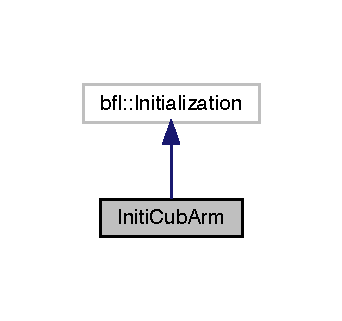
\includegraphics[width=164pt]{classInitiCubArm__inherit__graph}
\end{center}
\end{figure}
\subsection*{Public Member Functions}
\begin{DoxyCompactItemize}
\item 
\hyperlink{classInitiCubArm_aa59e8d0c6da59fcde27daec16e560cbf}{Initi\+Cub\+Arm} (const yarp\+::os\+::\+Const\+String \&port\+\_\+prefix, const yarp\+::os\+::\+Const\+String \&cam\+\_\+sel, const yarp\+::os\+::\+Const\+String \&laterality) noexcept
\item 
\hyperlink{classInitiCubArm_affa3e5d97a2f24f3e3fd2030a0dd5dbc}{Initi\+Cub\+Arm} (const yarp\+::os\+::\+Const\+String \&cam\+\_\+sel, const yarp\+::os\+::\+Const\+String \&laterality) noexcept
\item 
\hyperlink{classInitiCubArm_a337d96e7aecbd9235b3734c2aa317429}{$\sim$\+Initi\+Cub\+Arm} () noexcept
\item 
void \hyperlink{classInitiCubArm_a6f28c13828b5b90366b1105aef5820e3}{initialize} (Eigen\+::\+Ref$<$ Eigen\+::\+Matrix\+Xf $>$ state, Eigen\+::\+Ref$<$ Eigen\+::\+Vector\+Xf $>$ weight) override
\end{DoxyCompactItemize}
\subsection*{Private Member Functions}
\begin{DoxyCompactItemize}
\item 
yarp\+::sig\+::\+Vector \hyperlink{classInitiCubArm_a9e4667c1412ed80a44307fad5e553598}{read\+Torso} ()
\item 
yarp\+::sig\+::\+Vector \hyperlink{classInitiCubArm_a1dc997322826f47da11f6c247f86e063}{read\+Root\+To\+EE} ()
\end{DoxyCompactItemize}
\subsection*{Private Attributes}
\begin{DoxyCompactItemize}
\item 
i\+Cub\+::i\+Kin\+::i\+Cub\+Arm \hyperlink{classInitiCubArm_ae91a23c5ca3112d9a18561844ac0413b}{icub\+\_\+kin\+\_\+arm\+\_\+}
\item 
i\+Cub\+::i\+Kin\+::i\+Cub\+Finger \hyperlink{classInitiCubArm_a6fb2f21dcfe50b9d28bb58bc90c93f36}{icub\+\_\+kin\+\_\+finger\+\_\+} \mbox{[}3\mbox{]}
\item 
yarp\+::os\+::\+Buffered\+Port$<$ yarp\+::os\+::\+Bottle $>$ \hyperlink{classInitiCubArm_a1587e14242e40ec6cefaecfd1d88aff4}{port\+\_\+torso\+\_\+enc\+\_\+}
\item 
yarp\+::os\+::\+Buffered\+Port$<$ yarp\+::os\+::\+Bottle $>$ \hyperlink{classInitiCubArm_a0eb264a33270c599c0621b2148096516}{port\+\_\+arm\+\_\+enc\+\_\+}
\end{DoxyCompactItemize}


\subsection{Detailed Description}


Definition at line 12 of file Initi\+Cub\+Arm.\+h.



\subsection{Constructor \& Destructor Documentation}
\mbox{\Hypertarget{classInitiCubArm_aa59e8d0c6da59fcde27daec16e560cbf}\label{classInitiCubArm_aa59e8d0c6da59fcde27daec16e560cbf}} 
\index{Initi\+Cub\+Arm@{Initi\+Cub\+Arm}!Initi\+Cub\+Arm@{Initi\+Cub\+Arm}}
\index{Initi\+Cub\+Arm@{Initi\+Cub\+Arm}!Initi\+Cub\+Arm@{Initi\+Cub\+Arm}}
\subsubsection{\texorpdfstring{Initi\+Cub\+Arm()}{InitiCubArm()}\hspace{0.1cm}{\footnotesize\ttfamily [1/2]}}
{\footnotesize\ttfamily Initi\+Cub\+Arm\+::\+Initi\+Cub\+Arm (\begin{DoxyParamCaption}\item[{const yarp\+::os\+::\+Const\+String \&}]{port\+\_\+prefix,  }\item[{const yarp\+::os\+::\+Const\+String \&}]{cam\+\_\+sel,  }\item[{const yarp\+::os\+::\+Const\+String \&}]{laterality }\end{DoxyParamCaption})\hspace{0.3cm}{\ttfamily [noexcept]}}

\mbox{\Hypertarget{classInitiCubArm_affa3e5d97a2f24f3e3fd2030a0dd5dbc}\label{classInitiCubArm_affa3e5d97a2f24f3e3fd2030a0dd5dbc}} 
\index{Initi\+Cub\+Arm@{Initi\+Cub\+Arm}!Initi\+Cub\+Arm@{Initi\+Cub\+Arm}}
\index{Initi\+Cub\+Arm@{Initi\+Cub\+Arm}!Initi\+Cub\+Arm@{Initi\+Cub\+Arm}}
\subsubsection{\texorpdfstring{Initi\+Cub\+Arm()}{InitiCubArm()}\hspace{0.1cm}{\footnotesize\ttfamily [2/2]}}
{\footnotesize\ttfamily Initi\+Cub\+Arm\+::\+Initi\+Cub\+Arm (\begin{DoxyParamCaption}\item[{const yarp\+::os\+::\+Const\+String \&}]{cam\+\_\+sel,  }\item[{const yarp\+::os\+::\+Const\+String \&}]{laterality }\end{DoxyParamCaption})\hspace{0.3cm}{\ttfamily [noexcept]}}

\mbox{\Hypertarget{classInitiCubArm_a337d96e7aecbd9235b3734c2aa317429}\label{classInitiCubArm_a337d96e7aecbd9235b3734c2aa317429}} 
\index{Initi\+Cub\+Arm@{Initi\+Cub\+Arm}!````~Initi\+Cub\+Arm@{$\sim$\+Initi\+Cub\+Arm}}
\index{````~Initi\+Cub\+Arm@{$\sim$\+Initi\+Cub\+Arm}!Initi\+Cub\+Arm@{Initi\+Cub\+Arm}}
\subsubsection{\texorpdfstring{$\sim$\+Initi\+Cub\+Arm()}{~InitiCubArm()}}
{\footnotesize\ttfamily Initi\+Cub\+Arm\+::$\sim$\+Initi\+Cub\+Arm (\begin{DoxyParamCaption}{ }\end{DoxyParamCaption})\hspace{0.3cm}{\ttfamily [noexcept]}}



Definition at line 34 of file Initi\+Cub\+Arm.\+cpp.



\subsection{Member Function Documentation}
\mbox{\Hypertarget{classInitiCubArm_a6f28c13828b5b90366b1105aef5820e3}\label{classInitiCubArm_a6f28c13828b5b90366b1105aef5820e3}} 
\index{Initi\+Cub\+Arm@{Initi\+Cub\+Arm}!initialize@{initialize}}
\index{initialize@{initialize}!Initi\+Cub\+Arm@{Initi\+Cub\+Arm}}
\subsubsection{\texorpdfstring{initialize()}{initialize()}}
{\footnotesize\ttfamily void Initi\+Cub\+Arm\+::initialize (\begin{DoxyParamCaption}\item[{Eigen\+::\+Ref$<$ Eigen\+::\+Matrix\+Xf $>$}]{state,  }\item[{Eigen\+::\+Ref$<$ Eigen\+::\+Vector\+Xf $>$}]{weight }\end{DoxyParamCaption})\hspace{0.3cm}{\ttfamily [override]}}



Definition at line 41 of file Initi\+Cub\+Arm.\+cpp.

\mbox{\Hypertarget{classInitiCubArm_a1dc997322826f47da11f6c247f86e063}\label{classInitiCubArm_a1dc997322826f47da11f6c247f86e063}} 
\index{Initi\+Cub\+Arm@{Initi\+Cub\+Arm}!read\+Root\+To\+EE@{read\+Root\+To\+EE}}
\index{read\+Root\+To\+EE@{read\+Root\+To\+EE}!Initi\+Cub\+Arm@{Initi\+Cub\+Arm}}
\subsubsection{\texorpdfstring{read\+Root\+To\+E\+E()}{readRootToEE()}}
{\footnotesize\ttfamily Vector Initi\+Cub\+Arm\+::read\+Root\+To\+EE (\begin{DoxyParamCaption}{ }\end{DoxyParamCaption})\hspace{0.3cm}{\ttfamily [private]}}



Definition at line 68 of file Initi\+Cub\+Arm.\+cpp.

\mbox{\Hypertarget{classInitiCubArm_a9e4667c1412ed80a44307fad5e553598}\label{classInitiCubArm_a9e4667c1412ed80a44307fad5e553598}} 
\index{Initi\+Cub\+Arm@{Initi\+Cub\+Arm}!read\+Torso@{read\+Torso}}
\index{read\+Torso@{read\+Torso}!Initi\+Cub\+Arm@{Initi\+Cub\+Arm}}
\subsubsection{\texorpdfstring{read\+Torso()}{readTorso()}}
{\footnotesize\ttfamily Vector Initi\+Cub\+Arm\+::read\+Torso (\begin{DoxyParamCaption}{ }\end{DoxyParamCaption})\hspace{0.3cm}{\ttfamily [private]}}



Definition at line 54 of file Initi\+Cub\+Arm.\+cpp.



\subsection{Member Data Documentation}
\mbox{\Hypertarget{classInitiCubArm_ae91a23c5ca3112d9a18561844ac0413b}\label{classInitiCubArm_ae91a23c5ca3112d9a18561844ac0413b}} 
\index{Initi\+Cub\+Arm@{Initi\+Cub\+Arm}!icub\+\_\+kin\+\_\+arm\+\_\+@{icub\+\_\+kin\+\_\+arm\+\_\+}}
\index{icub\+\_\+kin\+\_\+arm\+\_\+@{icub\+\_\+kin\+\_\+arm\+\_\+}!Initi\+Cub\+Arm@{Initi\+Cub\+Arm}}
\subsubsection{\texorpdfstring{icub\+\_\+kin\+\_\+arm\+\_\+}{icub\_kin\_arm\_}}
{\footnotesize\ttfamily i\+Cub\+::i\+Kin\+::i\+Cub\+Arm Initi\+Cub\+Arm\+::icub\+\_\+kin\+\_\+arm\+\_\+\hspace{0.3cm}{\ttfamily [private]}}



Definition at line 24 of file Initi\+Cub\+Arm.\+h.

\mbox{\Hypertarget{classInitiCubArm_a6fb2f21dcfe50b9d28bb58bc90c93f36}\label{classInitiCubArm_a6fb2f21dcfe50b9d28bb58bc90c93f36}} 
\index{Initi\+Cub\+Arm@{Initi\+Cub\+Arm}!icub\+\_\+kin\+\_\+finger\+\_\+@{icub\+\_\+kin\+\_\+finger\+\_\+}}
\index{icub\+\_\+kin\+\_\+finger\+\_\+@{icub\+\_\+kin\+\_\+finger\+\_\+}!Initi\+Cub\+Arm@{Initi\+Cub\+Arm}}
\subsubsection{\texorpdfstring{icub\+\_\+kin\+\_\+finger\+\_\+}{icub\_kin\_finger\_}}
{\footnotesize\ttfamily i\+Cub\+::i\+Kin\+::i\+Cub\+Finger Initi\+Cub\+Arm\+::icub\+\_\+kin\+\_\+finger\+\_\+\mbox{[}3\mbox{]}\hspace{0.3cm}{\ttfamily [private]}}



Definition at line 25 of file Initi\+Cub\+Arm.\+h.

\mbox{\Hypertarget{classInitiCubArm_a0eb264a33270c599c0621b2148096516}\label{classInitiCubArm_a0eb264a33270c599c0621b2148096516}} 
\index{Initi\+Cub\+Arm@{Initi\+Cub\+Arm}!port\+\_\+arm\+\_\+enc\+\_\+@{port\+\_\+arm\+\_\+enc\+\_\+}}
\index{port\+\_\+arm\+\_\+enc\+\_\+@{port\+\_\+arm\+\_\+enc\+\_\+}!Initi\+Cub\+Arm@{Initi\+Cub\+Arm}}
\subsubsection{\texorpdfstring{port\+\_\+arm\+\_\+enc\+\_\+}{port\_arm\_enc\_}}
{\footnotesize\ttfamily yarp\+::os\+::\+Buffered\+Port$<$yarp\+::os\+::\+Bottle$>$ Initi\+Cub\+Arm\+::port\+\_\+arm\+\_\+enc\+\_\+\hspace{0.3cm}{\ttfamily [private]}}



Definition at line 27 of file Initi\+Cub\+Arm.\+h.

\mbox{\Hypertarget{classInitiCubArm_a1587e14242e40ec6cefaecfd1d88aff4}\label{classInitiCubArm_a1587e14242e40ec6cefaecfd1d88aff4}} 
\index{Initi\+Cub\+Arm@{Initi\+Cub\+Arm}!port\+\_\+torso\+\_\+enc\+\_\+@{port\+\_\+torso\+\_\+enc\+\_\+}}
\index{port\+\_\+torso\+\_\+enc\+\_\+@{port\+\_\+torso\+\_\+enc\+\_\+}!Initi\+Cub\+Arm@{Initi\+Cub\+Arm}}
\subsubsection{\texorpdfstring{port\+\_\+torso\+\_\+enc\+\_\+}{port\_torso\_enc\_}}
{\footnotesize\ttfamily yarp\+::os\+::\+Buffered\+Port$<$yarp\+::os\+::\+Bottle$>$ Initi\+Cub\+Arm\+::port\+\_\+torso\+\_\+enc\+\_\+\hspace{0.3cm}{\ttfamily [private]}}



Definition at line 26 of file Initi\+Cub\+Arm.\+h.



The documentation for this class was generated from the following files\+:\begin{DoxyCompactItemize}
\item 
/\+Users/\+Claudio/\+Git\+Hub/visual-\/tracking-\/control/src/hand-\/tracking/include/\hyperlink{InitiCubArm_8h}{Initi\+Cub\+Arm.\+h}\item 
/\+Users/\+Claudio/\+Git\+Hub/visual-\/tracking-\/control/src/hand-\/tracking/src/\hyperlink{InitiCubArm_8cpp}{Initi\+Cub\+Arm.\+cpp}\end{DoxyCompactItemize}

\hypertarget{classPlayFwdKinModel}{}\section{Play\+Fwd\+Kin\+Model Class Reference}
\label{classPlayFwdKinModel}\index{Play\+Fwd\+Kin\+Model@{Play\+Fwd\+Kin\+Model}}


{\ttfamily \#include $<$Play\+Fwd\+Kin\+Model.\+h$>$}



Inheritance diagram for Play\+Fwd\+Kin\+Model\+:
\nopagebreak
\begin{figure}[H]
\begin{center}
\leavevmode
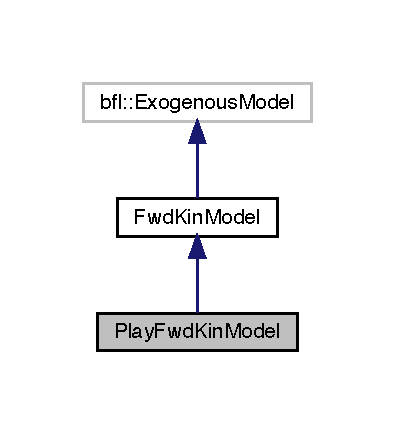
\includegraphics[width=189pt]{classPlayFwdKinModel__inherit__graph}
\end{center}
\end{figure}
\subsection*{Public Member Functions}
\begin{DoxyCompactItemize}
\item 
\hyperlink{classPlayFwdKinModel_aa7dbbe09aed1e7d1a1ac3fc37807f57c}{Play\+Fwd\+Kin\+Model} (const yarp\+::os\+::\+Const\+String \&robot, const yarp\+::os\+::\+Const\+String \&laterality, const yarp\+::os\+::\+Const\+String \&port\+\_\+prefix) noexcept
\item 
\hyperlink{classPlayFwdKinModel_a0af36404764e109bedacd8648939ba9c}{$\sim$\+Play\+Fwd\+Kin\+Model} () noexcept
\item 
bool \hyperlink{classPlayFwdKinModel_ae7f9432ed4f7069442821dbfa598321d}{set\+Property} (const std\+::string \&property) override
\item 
void \hyperlink{classFwdKinModel_a9461ff14a1ae8d05169e8f1c7a6237c7}{propagate} (const Eigen\+::\+Ref$<$ const Eigen\+::\+Matrix\+Xf $>$ \&cur\+\_\+state, Eigen\+::\+Ref$<$ Eigen\+::\+Matrix\+Xf $>$ prop\+\_\+state) override
\item 
Eigen\+::\+Matrix\+Xf \hyperlink{classFwdKinModel_ac8ed4e8a52f5ff33cc158c80c6cf083e}{get\+Exogenous\+Matrix} () override
\end{DoxyCompactItemize}
\subsection*{Protected Member Functions}
\begin{DoxyCompactItemize}
\item 
Eigen\+::\+Vector\+Xd \hyperlink{classPlayFwdKinModel_a282700bc69b26e6ea28cc5048881a599}{read\+Pose} () override
\item 
yarp\+::sig\+::\+Vector \hyperlink{classPlayFwdKinModel_a04170578030a5db53f7af45876b11492}{read\+Torso} ()
\item 
yarp\+::sig\+::\+Vector \hyperlink{classPlayFwdKinModel_a97e565b16712bb26a41fc78c4d1fca89}{read\+Root\+To\+EE} ()
\item 
bool \hyperlink{classFwdKinModel_a12b54bd62ba5cf218973c600c66ba39e}{set\+Delta\+Motion} ()
\end{DoxyCompactItemize}
\subsection*{Protected Attributes}
\begin{DoxyCompactItemize}
\item 
yarp\+::os\+::\+Buffered\+Port$<$ yarp\+::os\+::\+Bottle $>$ \hyperlink{classPlayFwdKinModel_a092cea2f9523b8f303fded1067e2f965}{port\+\_\+torso\+\_\+enc\+\_\+}
\item 
yarp\+::os\+::\+Buffered\+Port$<$ yarp\+::os\+::\+Bottle $>$ \hyperlink{classPlayFwdKinModel_abe0b6fcb827b0c1c0b07ad083eb224e6}{port\+\_\+arm\+\_\+enc\+\_\+}
\item 
i\+Cub\+::i\+Kin\+::i\+Cub\+Arm \hyperlink{classPlayFwdKinModel_af6e5c3ce282a1326b7d58e45c68412a9}{icub\+\_\+kin\+\_\+arm\+\_\+}
\item 
bool \hyperlink{classFwdKinModel_a2ed7b77ebd710e5debe63b83a34a1645}{initialize\+\_\+delta\+\_\+} = true
\end{DoxyCompactItemize}
\subsection*{Private Attributes}
\begin{DoxyCompactItemize}
\item 
yarp\+::os\+::\+Const\+String \hyperlink{classPlayFwdKinModel_a2e37370f9958d7b77bc1377ede99d554}{I\+D\+\_\+} = \char`\"{}Play\+Fwd\+Kin\+Model\char`\"{}
\item 
yarp\+::os\+::\+Const\+String \hyperlink{classPlayFwdKinModel_a8e6132483f92deaed9ad1c529d398673}{log\+\_\+\+I\+D\+\_\+} = \char`\"{}\mbox{[}\char`\"{} + \hyperlink{classPlayFwdKinModel_a2e37370f9958d7b77bc1377ede99d554}{I\+D\+\_\+} + \char`\"{}\mbox{]}\char`\"{}
\item 
yarp\+::os\+::\+Const\+String \hyperlink{classPlayFwdKinModel_acb83b9edcd4d111ff6f295f26796351d}{robot\+\_\+}
\item 
yarp\+::os\+::\+Const\+String \hyperlink{classPlayFwdKinModel_a9066d4c54a62b989be77ab29a0b65f93}{laterality\+\_\+}
\item 
yarp\+::os\+::\+Const\+String \hyperlink{classPlayFwdKinModel_adcde73c93a3e42a6b444db742d9d50af}{port\+\_\+prefix\+\_\+}
\end{DoxyCompactItemize}


\subsection{Detailed Description}


Definition at line 13 of file Play\+Fwd\+Kin\+Model.\+h.



\subsection{Constructor \& Destructor Documentation}
\mbox{\Hypertarget{classPlayFwdKinModel_aa7dbbe09aed1e7d1a1ac3fc37807f57c}\label{classPlayFwdKinModel_aa7dbbe09aed1e7d1a1ac3fc37807f57c}} 
\index{Play\+Fwd\+Kin\+Model@{Play\+Fwd\+Kin\+Model}!Play\+Fwd\+Kin\+Model@{Play\+Fwd\+Kin\+Model}}
\index{Play\+Fwd\+Kin\+Model@{Play\+Fwd\+Kin\+Model}!Play\+Fwd\+Kin\+Model@{Play\+Fwd\+Kin\+Model}}
\subsubsection{\texorpdfstring{Play\+Fwd\+Kin\+Model()}{PlayFwdKinModel()}}
{\footnotesize\ttfamily Play\+Fwd\+Kin\+Model\+::\+Play\+Fwd\+Kin\+Model (\begin{DoxyParamCaption}\item[{const yarp\+::os\+::\+Const\+String \&}]{robot,  }\item[{const yarp\+::os\+::\+Const\+String \&}]{laterality,  }\item[{const yarp\+::os\+::\+Const\+String \&}]{port\+\_\+prefix }\end{DoxyParamCaption})\hspace{0.3cm}{\ttfamily [noexcept]}}



Definition at line 23 of file Play\+Fwd\+Kin\+Model.\+cpp.

\mbox{\Hypertarget{classPlayFwdKinModel_a0af36404764e109bedacd8648939ba9c}\label{classPlayFwdKinModel_a0af36404764e109bedacd8648939ba9c}} 
\index{Play\+Fwd\+Kin\+Model@{Play\+Fwd\+Kin\+Model}!````~Play\+Fwd\+Kin\+Model@{$\sim$\+Play\+Fwd\+Kin\+Model}}
\index{````~Play\+Fwd\+Kin\+Model@{$\sim$\+Play\+Fwd\+Kin\+Model}!Play\+Fwd\+Kin\+Model@{Play\+Fwd\+Kin\+Model}}
\subsubsection{\texorpdfstring{$\sim$\+Play\+Fwd\+Kin\+Model()}{~PlayFwdKinModel()}}
{\footnotesize\ttfamily Play\+Fwd\+Kin\+Model\+::$\sim$\+Play\+Fwd\+Kin\+Model (\begin{DoxyParamCaption}{ }\end{DoxyParamCaption})\hspace{0.3cm}{\ttfamily [noexcept]}}



Definition at line 38 of file Play\+Fwd\+Kin\+Model.\+cpp.



\subsection{Member Function Documentation}
\mbox{\Hypertarget{classFwdKinModel_ac8ed4e8a52f5ff33cc158c80c6cf083e}\label{classFwdKinModel_ac8ed4e8a52f5ff33cc158c80c6cf083e}} 
\index{Play\+Fwd\+Kin\+Model@{Play\+Fwd\+Kin\+Model}!get\+Exogenous\+Matrix@{get\+Exogenous\+Matrix}}
\index{get\+Exogenous\+Matrix@{get\+Exogenous\+Matrix}!Play\+Fwd\+Kin\+Model@{Play\+Fwd\+Kin\+Model}}
\subsubsection{\texorpdfstring{get\+Exogenous\+Matrix()}{getExogenousMatrix()}}
{\footnotesize\ttfamily Matrix\+Xf Fwd\+Kin\+Model\+::get\+Exogenous\+Matrix (\begin{DoxyParamCaption}{ }\end{DoxyParamCaption})\hspace{0.3cm}{\ttfamily [override]}, {\ttfamily [inherited]}}



Definition at line 47 of file Fwd\+Kin\+Model.\+cpp.

\mbox{\Hypertarget{classFwdKinModel_a9461ff14a1ae8d05169e8f1c7a6237c7}\label{classFwdKinModel_a9461ff14a1ae8d05169e8f1c7a6237c7}} 
\index{Play\+Fwd\+Kin\+Model@{Play\+Fwd\+Kin\+Model}!propagate@{propagate}}
\index{propagate@{propagate}!Play\+Fwd\+Kin\+Model@{Play\+Fwd\+Kin\+Model}}
\subsubsection{\texorpdfstring{propagate()}{propagate()}}
{\footnotesize\ttfamily void Fwd\+Kin\+Model\+::propagate (\begin{DoxyParamCaption}\item[{const Eigen\+::\+Ref$<$ const Eigen\+::\+Matrix\+Xf $>$ \&}]{cur\+\_\+state,  }\item[{Eigen\+::\+Ref$<$ Eigen\+::\+Matrix\+Xf $>$}]{prop\+\_\+state }\end{DoxyParamCaption})\hspace{0.3cm}{\ttfamily [override]}, {\ttfamily [inherited]}}



Definition at line 28 of file Fwd\+Kin\+Model.\+cpp.

\mbox{\Hypertarget{classPlayFwdKinModel_a282700bc69b26e6ea28cc5048881a599}\label{classPlayFwdKinModel_a282700bc69b26e6ea28cc5048881a599}} 
\index{Play\+Fwd\+Kin\+Model@{Play\+Fwd\+Kin\+Model}!read\+Pose@{read\+Pose}}
\index{read\+Pose@{read\+Pose}!Play\+Fwd\+Kin\+Model@{Play\+Fwd\+Kin\+Model}}
\subsubsection{\texorpdfstring{read\+Pose()}{readPose()}}
{\footnotesize\ttfamily Vector\+Xd Play\+Fwd\+Kin\+Model\+::read\+Pose (\begin{DoxyParamCaption}{ }\end{DoxyParamCaption})\hspace{0.3cm}{\ttfamily [override]}, {\ttfamily [protected]}, {\ttfamily [virtual]}}



Implements \hyperlink{classFwdKinModel_aaad9ff96f725fc529672e12aed86dc02}{Fwd\+Kin\+Model}.



Definition at line 54 of file Play\+Fwd\+Kin\+Model.\+cpp.

\mbox{\Hypertarget{classPlayFwdKinModel_a97e565b16712bb26a41fc78c4d1fca89}\label{classPlayFwdKinModel_a97e565b16712bb26a41fc78c4d1fca89}} 
\index{Play\+Fwd\+Kin\+Model@{Play\+Fwd\+Kin\+Model}!read\+Root\+To\+EE@{read\+Root\+To\+EE}}
\index{read\+Root\+To\+EE@{read\+Root\+To\+EE}!Play\+Fwd\+Kin\+Model@{Play\+Fwd\+Kin\+Model}}
\subsubsection{\texorpdfstring{read\+Root\+To\+E\+E()}{readRootToEE()}}
{\footnotesize\ttfamily Vector Play\+Fwd\+Kin\+Model\+::read\+Root\+To\+EE (\begin{DoxyParamCaption}{ }\end{DoxyParamCaption})\hspace{0.3cm}{\ttfamily [protected]}}



Definition at line 75 of file Play\+Fwd\+Kin\+Model.\+cpp.

\mbox{\Hypertarget{classPlayFwdKinModel_a04170578030a5db53f7af45876b11492}\label{classPlayFwdKinModel_a04170578030a5db53f7af45876b11492}} 
\index{Play\+Fwd\+Kin\+Model@{Play\+Fwd\+Kin\+Model}!read\+Torso@{read\+Torso}}
\index{read\+Torso@{read\+Torso}!Play\+Fwd\+Kin\+Model@{Play\+Fwd\+Kin\+Model}}
\subsubsection{\texorpdfstring{read\+Torso()}{readTorso()}}
{\footnotesize\ttfamily Vector Play\+Fwd\+Kin\+Model\+::read\+Torso (\begin{DoxyParamCaption}{ }\end{DoxyParamCaption})\hspace{0.3cm}{\ttfamily [protected]}}



Definition at line 61 of file Play\+Fwd\+Kin\+Model.\+cpp.

\mbox{\Hypertarget{classFwdKinModel_a12b54bd62ba5cf218973c600c66ba39e}\label{classFwdKinModel_a12b54bd62ba5cf218973c600c66ba39e}} 
\index{Play\+Fwd\+Kin\+Model@{Play\+Fwd\+Kin\+Model}!set\+Delta\+Motion@{set\+Delta\+Motion}}
\index{set\+Delta\+Motion@{set\+Delta\+Motion}!Play\+Fwd\+Kin\+Model@{Play\+Fwd\+Kin\+Model}}
\subsubsection{\texorpdfstring{set\+Delta\+Motion()}{setDeltaMotion()}}
{\footnotesize\ttfamily bool Fwd\+Kin\+Model\+::set\+Delta\+Motion (\begin{DoxyParamCaption}{ }\end{DoxyParamCaption})\hspace{0.3cm}{\ttfamily [protected]}, {\ttfamily [inherited]}}



Definition at line 71 of file Fwd\+Kin\+Model.\+cpp.

\mbox{\Hypertarget{classPlayFwdKinModel_ae7f9432ed4f7069442821dbfa598321d}\label{classPlayFwdKinModel_ae7f9432ed4f7069442821dbfa598321d}} 
\index{Play\+Fwd\+Kin\+Model@{Play\+Fwd\+Kin\+Model}!set\+Property@{set\+Property}}
\index{set\+Property@{set\+Property}!Play\+Fwd\+Kin\+Model@{Play\+Fwd\+Kin\+Model}}
\subsubsection{\texorpdfstring{set\+Property()}{setProperty()}}
{\footnotesize\ttfamily bool Play\+Fwd\+Kin\+Model\+::set\+Property (\begin{DoxyParamCaption}\item[{const std\+::string \&}]{property }\end{DoxyParamCaption})\hspace{0.3cm}{\ttfamily [override]}}



Definition at line 48 of file Play\+Fwd\+Kin\+Model.\+cpp.



References Fwd\+Kin\+Model\+::set\+Property().

Here is the call graph for this function\+:
\nopagebreak
\begin{figure}[H]
\begin{center}
\leavevmode
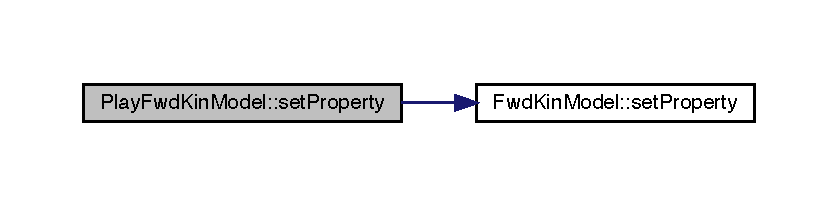
\includegraphics[width=350pt]{classPlayFwdKinModel_ae7f9432ed4f7069442821dbfa598321d_cgraph}
\end{center}
\end{figure}


\subsection{Member Data Documentation}
\mbox{\Hypertarget{classPlayFwdKinModel_af6e5c3ce282a1326b7d58e45c68412a9}\label{classPlayFwdKinModel_af6e5c3ce282a1326b7d58e45c68412a9}} 
\index{Play\+Fwd\+Kin\+Model@{Play\+Fwd\+Kin\+Model}!icub\+\_\+kin\+\_\+arm\+\_\+@{icub\+\_\+kin\+\_\+arm\+\_\+}}
\index{icub\+\_\+kin\+\_\+arm\+\_\+@{icub\+\_\+kin\+\_\+arm\+\_\+}!Play\+Fwd\+Kin\+Model@{Play\+Fwd\+Kin\+Model}}
\subsubsection{\texorpdfstring{icub\+\_\+kin\+\_\+arm\+\_\+}{icub\_kin\_arm\_}}
{\footnotesize\ttfamily i\+Cub\+::i\+Kin\+::i\+Cub\+Arm Play\+Fwd\+Kin\+Model\+::icub\+\_\+kin\+\_\+arm\+\_\+\hspace{0.3cm}{\ttfamily [protected]}}



Definition at line 31 of file Play\+Fwd\+Kin\+Model.\+h.

\mbox{\Hypertarget{classPlayFwdKinModel_a2e37370f9958d7b77bc1377ede99d554}\label{classPlayFwdKinModel_a2e37370f9958d7b77bc1377ede99d554}} 
\index{Play\+Fwd\+Kin\+Model@{Play\+Fwd\+Kin\+Model}!I\+D\+\_\+@{I\+D\+\_\+}}
\index{I\+D\+\_\+@{I\+D\+\_\+}!Play\+Fwd\+Kin\+Model@{Play\+Fwd\+Kin\+Model}}
\subsubsection{\texorpdfstring{I\+D\+\_\+}{ID\_}}
{\footnotesize\ttfamily yarp\+::os\+::\+Const\+String Play\+Fwd\+Kin\+Model\+::\+I\+D\+\_\+ = \char`\"{}Play\+Fwd\+Kin\+Model\char`\"{}\hspace{0.3cm}{\ttfamily [private]}}



Definition at line 34 of file Play\+Fwd\+Kin\+Model.\+h.

\mbox{\Hypertarget{classFwdKinModel_a2ed7b77ebd710e5debe63b83a34a1645}\label{classFwdKinModel_a2ed7b77ebd710e5debe63b83a34a1645}} 
\index{Play\+Fwd\+Kin\+Model@{Play\+Fwd\+Kin\+Model}!initialize\+\_\+delta\+\_\+@{initialize\+\_\+delta\+\_\+}}
\index{initialize\+\_\+delta\+\_\+@{initialize\+\_\+delta\+\_\+}!Play\+Fwd\+Kin\+Model@{Play\+Fwd\+Kin\+Model}}
\subsubsection{\texorpdfstring{initialize\+\_\+delta\+\_\+}{initialize\_delta\_}}
{\footnotesize\ttfamily bool Fwd\+Kin\+Model\+::initialize\+\_\+delta\+\_\+ = true\hspace{0.3cm}{\ttfamily [protected]}, {\ttfamily [inherited]}}



Definition at line 28 of file Fwd\+Kin\+Model.\+h.

\mbox{\Hypertarget{classPlayFwdKinModel_a9066d4c54a62b989be77ab29a0b65f93}\label{classPlayFwdKinModel_a9066d4c54a62b989be77ab29a0b65f93}} 
\index{Play\+Fwd\+Kin\+Model@{Play\+Fwd\+Kin\+Model}!laterality\+\_\+@{laterality\+\_\+}}
\index{laterality\+\_\+@{laterality\+\_\+}!Play\+Fwd\+Kin\+Model@{Play\+Fwd\+Kin\+Model}}
\subsubsection{\texorpdfstring{laterality\+\_\+}{laterality\_}}
{\footnotesize\ttfamily yarp\+::os\+::\+Const\+String Play\+Fwd\+Kin\+Model\+::laterality\+\_\+\hspace{0.3cm}{\ttfamily [private]}}



Definition at line 38 of file Play\+Fwd\+Kin\+Model.\+h.

\mbox{\Hypertarget{classPlayFwdKinModel_a8e6132483f92deaed9ad1c529d398673}\label{classPlayFwdKinModel_a8e6132483f92deaed9ad1c529d398673}} 
\index{Play\+Fwd\+Kin\+Model@{Play\+Fwd\+Kin\+Model}!log\+\_\+\+I\+D\+\_\+@{log\+\_\+\+I\+D\+\_\+}}
\index{log\+\_\+\+I\+D\+\_\+@{log\+\_\+\+I\+D\+\_\+}!Play\+Fwd\+Kin\+Model@{Play\+Fwd\+Kin\+Model}}
\subsubsection{\texorpdfstring{log\+\_\+\+I\+D\+\_\+}{log\_ID\_}}
{\footnotesize\ttfamily yarp\+::os\+::\+Const\+String Play\+Fwd\+Kin\+Model\+::log\+\_\+\+I\+D\+\_\+ = \char`\"{}\mbox{[}\char`\"{} + \hyperlink{classPlayFwdKinModel_a2e37370f9958d7b77bc1377ede99d554}{I\+D\+\_\+} + \char`\"{}\mbox{]}\char`\"{}\hspace{0.3cm}{\ttfamily [private]}}



Definition at line 35 of file Play\+Fwd\+Kin\+Model.\+h.

\mbox{\Hypertarget{classPlayFwdKinModel_abe0b6fcb827b0c1c0b07ad083eb224e6}\label{classPlayFwdKinModel_abe0b6fcb827b0c1c0b07ad083eb224e6}} 
\index{Play\+Fwd\+Kin\+Model@{Play\+Fwd\+Kin\+Model}!port\+\_\+arm\+\_\+enc\+\_\+@{port\+\_\+arm\+\_\+enc\+\_\+}}
\index{port\+\_\+arm\+\_\+enc\+\_\+@{port\+\_\+arm\+\_\+enc\+\_\+}!Play\+Fwd\+Kin\+Model@{Play\+Fwd\+Kin\+Model}}
\subsubsection{\texorpdfstring{port\+\_\+arm\+\_\+enc\+\_\+}{port\_arm\_enc\_}}
{\footnotesize\ttfamily yarp\+::os\+::\+Buffered\+Port$<$yarp\+::os\+::\+Bottle$>$ Play\+Fwd\+Kin\+Model\+::port\+\_\+arm\+\_\+enc\+\_\+\hspace{0.3cm}{\ttfamily [protected]}}



Definition at line 30 of file Play\+Fwd\+Kin\+Model.\+h.

\mbox{\Hypertarget{classPlayFwdKinModel_adcde73c93a3e42a6b444db742d9d50af}\label{classPlayFwdKinModel_adcde73c93a3e42a6b444db742d9d50af}} 
\index{Play\+Fwd\+Kin\+Model@{Play\+Fwd\+Kin\+Model}!port\+\_\+prefix\+\_\+@{port\+\_\+prefix\+\_\+}}
\index{port\+\_\+prefix\+\_\+@{port\+\_\+prefix\+\_\+}!Play\+Fwd\+Kin\+Model@{Play\+Fwd\+Kin\+Model}}
\subsubsection{\texorpdfstring{port\+\_\+prefix\+\_\+}{port\_prefix\_}}
{\footnotesize\ttfamily yarp\+::os\+::\+Const\+String Play\+Fwd\+Kin\+Model\+::port\+\_\+prefix\+\_\+\hspace{0.3cm}{\ttfamily [private]}}



Definition at line 39 of file Play\+Fwd\+Kin\+Model.\+h.

\mbox{\Hypertarget{classPlayFwdKinModel_a092cea2f9523b8f303fded1067e2f965}\label{classPlayFwdKinModel_a092cea2f9523b8f303fded1067e2f965}} 
\index{Play\+Fwd\+Kin\+Model@{Play\+Fwd\+Kin\+Model}!port\+\_\+torso\+\_\+enc\+\_\+@{port\+\_\+torso\+\_\+enc\+\_\+}}
\index{port\+\_\+torso\+\_\+enc\+\_\+@{port\+\_\+torso\+\_\+enc\+\_\+}!Play\+Fwd\+Kin\+Model@{Play\+Fwd\+Kin\+Model}}
\subsubsection{\texorpdfstring{port\+\_\+torso\+\_\+enc\+\_\+}{port\_torso\_enc\_}}
{\footnotesize\ttfamily yarp\+::os\+::\+Buffered\+Port$<$yarp\+::os\+::\+Bottle$>$ Play\+Fwd\+Kin\+Model\+::port\+\_\+torso\+\_\+enc\+\_\+\hspace{0.3cm}{\ttfamily [protected]}}



Definition at line 29 of file Play\+Fwd\+Kin\+Model.\+h.

\mbox{\Hypertarget{classPlayFwdKinModel_acb83b9edcd4d111ff6f295f26796351d}\label{classPlayFwdKinModel_acb83b9edcd4d111ff6f295f26796351d}} 
\index{Play\+Fwd\+Kin\+Model@{Play\+Fwd\+Kin\+Model}!robot\+\_\+@{robot\+\_\+}}
\index{robot\+\_\+@{robot\+\_\+}!Play\+Fwd\+Kin\+Model@{Play\+Fwd\+Kin\+Model}}
\subsubsection{\texorpdfstring{robot\+\_\+}{robot\_}}
{\footnotesize\ttfamily yarp\+::os\+::\+Const\+String Play\+Fwd\+Kin\+Model\+::robot\+\_\+\hspace{0.3cm}{\ttfamily [private]}}



Definition at line 37 of file Play\+Fwd\+Kin\+Model.\+h.



The documentation for this class was generated from the following files\+:\begin{DoxyCompactItemize}
\item 
/\+Users/\+Claudio/\+Git\+Hub/visual-\/tracking-\/control/src/hand-\/tracking/include/\hyperlink{PlayFwdKinModel_8h}{Play\+Fwd\+Kin\+Model.\+h}\item 
/\+Users/\+Claudio/\+Git\+Hub/visual-\/tracking-\/control/src/hand-\/tracking/src/\hyperlink{PlayFwdKinModel_8cpp}{Play\+Fwd\+Kin\+Model.\+cpp}\end{DoxyCompactItemize}

\hypertarget{classPlayGatePose}{}\section{Play\+Gate\+Pose Class Reference}
\label{classPlayGatePose}\index{Play\+Gate\+Pose@{Play\+Gate\+Pose}}


{\ttfamily \#include $<$Play\+Gate\+Pose.\+h$>$}



Inheritance diagram for Play\+Gate\+Pose\+:
\nopagebreak
\begin{figure}[H]
\begin{center}
\leavevmode
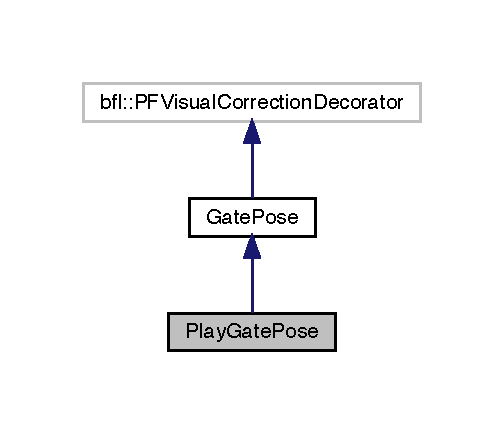
\includegraphics[width=242pt]{classPlayGatePose__inherit__graph}
\end{center}
\end{figure}
\subsection*{Public Member Functions}
\begin{DoxyCompactItemize}
\item 
\hyperlink{classPlayGatePose_a134d268932fcced2e6d6cc1a800cf7e9}{Play\+Gate\+Pose} (std\+::unique\+\_\+ptr$<$ P\+F\+Visual\+Correction $>$ visual\+\_\+correction, const double gate\+\_\+x, const double gate\+\_\+y, const double gate\+\_\+z, const double gate\+\_\+aperture, const double gate\+\_\+rotation, const yarp\+::os\+::\+Const\+String \&robot, const yarp\+::os\+::\+Const\+String \&laterality, const yarp\+::os\+::\+Const\+String \&port\+\_\+prefix) noexcept
\item 
\hyperlink{classPlayGatePose_a8fdd90dc3b3f2b4c2f93e31d11aaabce}{Play\+Gate\+Pose} (std\+::unique\+\_\+ptr$<$ P\+F\+Visual\+Correction $>$ visual\+\_\+correction, const yarp\+::os\+::\+Const\+String \&robot, const yarp\+::os\+::\+Const\+String \&laterality, const yarp\+::os\+::\+Const\+String \&port\+\_\+prefix) noexcept
\item 
\hyperlink{classPlayGatePose_a06fd05c14cdfc88a04a7d860c7c66bf6}{$\sim$\+Play\+Gate\+Pose} () noexcept override
\item 
void \hyperlink{classGatePose_a00607a4325dcfb7a02bda7490b65d25c}{innovation} (const Eigen\+::\+Ref$<$ const Eigen\+::\+Matrix\+Xf $>$ \&pred\+\_\+states, cv\+::\+Input\+Array measurements, Eigen\+::\+Ref$<$ Eigen\+::\+Matrix\+Xf $>$ innovations) override
\item 
double \hyperlink{classGatePose_a939c575d5d59c8b0f3ab528edd368c0d}{likelihood} (const Eigen\+::\+Ref$<$ const Eigen\+::\+Matrix\+Xf $>$ \&innovations) override
\item 
bfl\+::\+Visual\+Observation\+Model \& \hyperlink{classGatePose_aa47f9242f039b8752675db5594350a28}{get\+Visual\+Observation\+Model} () override
\item 
void \hyperlink{classGatePose_a18ba358c801ae1a246dbee2f9780c698}{set\+Visual\+Observation\+Model} (std\+::unique\+\_\+ptr$<$ bfl\+::\+Visual\+Observation\+Model $>$ visual\+\_\+observation\+\_\+model) override
\end{DoxyCompactItemize}
\subsection*{Protected Member Functions}
\begin{DoxyCompactItemize}
\item 
Eigen\+::\+Vector\+Xd \hyperlink{classPlayGatePose_a863afa00ea83395e7f2ceffd26242106}{read\+Pose} () override
\item 
yarp\+::sig\+::\+Vector \hyperlink{classPlayGatePose_aa9304fb7f500dc947d5e2b5687fa2caf}{read\+Root\+To\+EE} ()
\item 
yarp\+::sig\+::\+Vector \hyperlink{classPlayGatePose_a9df2350244234bbd6cd3e32d2592eca4}{read\+Torso} ()
\item 
void \hyperlink{classGatePose_a91d395abe75dc7772116f50219dc19ae}{correct\+Step} (const Eigen\+::\+Ref$<$ const Eigen\+::\+Matrix\+Xf $>$ \&pred\+\_\+states, const Eigen\+::\+Ref$<$ const Eigen\+::\+Vector\+Xf $>$ \&pred\+\_\+weights, cv\+::\+Input\+Array measurements, Eigen\+::\+Ref$<$ Eigen\+::\+Matrix\+Xf $>$ cor\+\_\+states, Eigen\+::\+Ref$<$ Eigen\+::\+Vector\+Xf $>$ cor\+\_\+weights) override
\item 
bool \hyperlink{classGatePose_a880273787b1b3542e1e7971954ac118d}{is\+Inside\+Ellipsoid} (const Eigen\+::\+Ref$<$ const Eigen\+::\+Vector\+Xf $>$ \&state)
\item 
bool \hyperlink{classGatePose_a6d188756ed5dcc56c311a2aafc9d1acd}{is\+Within\+Rotation} (float rot\+\_\+angle)
\item 
bool \hyperlink{classGatePose_ad2e8708b3ed5a8252bdec1494f199fda}{is\+Inside\+Cone} (const Eigen\+::\+Ref$<$ const Eigen\+::\+Vector\+Xf $>$ \&state)
\end{DoxyCompactItemize}
\subsection*{Protected Attributes}
\begin{DoxyCompactItemize}
\item 
yarp\+::os\+::\+Buffered\+Port$<$ yarp\+::os\+::\+Bottle $>$ \hyperlink{classPlayGatePose_a95364e89c1f231c8f1c6c446c59c60a1}{port\+\_\+torso\+\_\+enc\+\_\+}
\item 
yarp\+::os\+::\+Buffered\+Port$<$ yarp\+::os\+::\+Bottle $>$ \hyperlink{classPlayGatePose_a5ca90c285338480d1107dafff024ffa6}{port\+\_\+arm\+\_\+enc\+\_\+}
\item 
i\+Cub\+::i\+Kin\+::i\+Cub\+Arm \hyperlink{classPlayGatePose_aa108b754575bdc988508a78c779de9da}{icub\+\_\+kin\+\_\+arm\+\_\+}
\end{DoxyCompactItemize}
\subsection*{Private Attributes}
\begin{DoxyCompactItemize}
\item 
const yarp\+::os\+::\+Const\+String \hyperlink{classPlayGatePose_a8700d03eb31893c2dd629b6428edcf8f}{I\+D\+\_\+} = \char`\"{}Play\+Gate\+Pose\char`\"{}
\item 
const yarp\+::os\+::\+Const\+String \hyperlink{classPlayGatePose_a45dc28ee85b9ea1d885d0a62f5dc4d81}{log\+\_\+\+I\+D\+\_\+} = \char`\"{}\mbox{[}\char`\"{} + \hyperlink{classPlayGatePose_a8700d03eb31893c2dd629b6428edcf8f}{I\+D\+\_\+} + \char`\"{}\mbox{]}\char`\"{}
\item 
yarp\+::os\+::\+Const\+String \hyperlink{classPlayGatePose_aa4015d529ba3c0cb9306e2c67cec3bb2}{robot\+\_\+}
\item 
yarp\+::os\+::\+Const\+String \hyperlink{classPlayGatePose_aed3a573d0e4a96673e49066dff1526e3}{laterality\+\_\+}
\item 
yarp\+::os\+::\+Const\+String \hyperlink{classPlayGatePose_a14886233558f20f775b6fbb523f14566}{port\+\_\+prefix\+\_\+}
\end{DoxyCompactItemize}


\subsection{Detailed Description}


Definition at line 12 of file Play\+Gate\+Pose.\+h.



\subsection{Constructor \& Destructor Documentation}
\mbox{\Hypertarget{classPlayGatePose_a134d268932fcced2e6d6cc1a800cf7e9}\label{classPlayGatePose_a134d268932fcced2e6d6cc1a800cf7e9}} 
\index{Play\+Gate\+Pose@{Play\+Gate\+Pose}!Play\+Gate\+Pose@{Play\+Gate\+Pose}}
\index{Play\+Gate\+Pose@{Play\+Gate\+Pose}!Play\+Gate\+Pose@{Play\+Gate\+Pose}}
\subsubsection{\texorpdfstring{Play\+Gate\+Pose()}{PlayGatePose()}\hspace{0.1cm}{\footnotesize\ttfamily [1/2]}}
{\footnotesize\ttfamily Play\+Gate\+Pose\+::\+Play\+Gate\+Pose (\begin{DoxyParamCaption}\item[{std\+::unique\+\_\+ptr$<$ P\+F\+Visual\+Correction $>$}]{visual\+\_\+correction,  }\item[{const double}]{gate\+\_\+x,  }\item[{const double}]{gate\+\_\+y,  }\item[{const double}]{gate\+\_\+z,  }\item[{const double}]{gate\+\_\+aperture,  }\item[{const double}]{gate\+\_\+rotation,  }\item[{const yarp\+::os\+::\+Const\+String \&}]{robot,  }\item[{const yarp\+::os\+::\+Const\+String \&}]{laterality,  }\item[{const yarp\+::os\+::\+Const\+String \&}]{port\+\_\+prefix }\end{DoxyParamCaption})\hspace{0.3cm}{\ttfamily [noexcept]}}



Definition at line 19 of file Play\+Gate\+Pose.\+cpp.

\mbox{\Hypertarget{classPlayGatePose_a8fdd90dc3b3f2b4c2f93e31d11aaabce}\label{classPlayGatePose_a8fdd90dc3b3f2b4c2f93e31d11aaabce}} 
\index{Play\+Gate\+Pose@{Play\+Gate\+Pose}!Play\+Gate\+Pose@{Play\+Gate\+Pose}}
\index{Play\+Gate\+Pose@{Play\+Gate\+Pose}!Play\+Gate\+Pose@{Play\+Gate\+Pose}}
\subsubsection{\texorpdfstring{Play\+Gate\+Pose()}{PlayGatePose()}\hspace{0.1cm}{\footnotesize\ttfamily [2/2]}}
{\footnotesize\ttfamily Play\+Gate\+Pose\+::\+Play\+Gate\+Pose (\begin{DoxyParamCaption}\item[{std\+::unique\+\_\+ptr$<$ P\+F\+Visual\+Correction $>$}]{visual\+\_\+correction,  }\item[{const yarp\+::os\+::\+Const\+String \&}]{robot,  }\item[{const yarp\+::os\+::\+Const\+String \&}]{laterality,  }\item[{const yarp\+::os\+::\+Const\+String \&}]{port\+\_\+prefix }\end{DoxyParamCaption})\hspace{0.3cm}{\ttfamily [noexcept]}}



Definition at line 44 of file Play\+Gate\+Pose.\+cpp.

\mbox{\Hypertarget{classPlayGatePose_a06fd05c14cdfc88a04a7d860c7c66bf6}\label{classPlayGatePose_a06fd05c14cdfc88a04a7d860c7c66bf6}} 
\index{Play\+Gate\+Pose@{Play\+Gate\+Pose}!````~Play\+Gate\+Pose@{$\sim$\+Play\+Gate\+Pose}}
\index{````~Play\+Gate\+Pose@{$\sim$\+Play\+Gate\+Pose}!Play\+Gate\+Pose@{Play\+Gate\+Pose}}
\subsubsection{\texorpdfstring{$\sim$\+Play\+Gate\+Pose()}{~PlayGatePose()}}
{\footnotesize\ttfamily Play\+Gate\+Pose\+::$\sim$\+Play\+Gate\+Pose (\begin{DoxyParamCaption}{ }\end{DoxyParamCaption})\hspace{0.3cm}{\ttfamily [override]}, {\ttfamily [noexcept]}}



Definition at line 49 of file Play\+Gate\+Pose.\+cpp.



\subsection{Member Function Documentation}
\mbox{\Hypertarget{classGatePose_a91d395abe75dc7772116f50219dc19ae}\label{classGatePose_a91d395abe75dc7772116f50219dc19ae}} 
\index{Play\+Gate\+Pose@{Play\+Gate\+Pose}!correct\+Step@{correct\+Step}}
\index{correct\+Step@{correct\+Step}!Play\+Gate\+Pose@{Play\+Gate\+Pose}}
\subsubsection{\texorpdfstring{correct\+Step()}{correctStep()}}
{\footnotesize\ttfamily void Gate\+Pose\+::correct\+Step (\begin{DoxyParamCaption}\item[{const Eigen\+::\+Ref$<$ const Eigen\+::\+Matrix\+Xf $>$ \&}]{pred\+\_\+states,  }\item[{const Eigen\+::\+Ref$<$ const Eigen\+::\+Vector\+Xf $>$ \&}]{pred\+\_\+weights,  }\item[{cv\+::\+Input\+Array}]{measurements,  }\item[{Eigen\+::\+Ref$<$ Eigen\+::\+Matrix\+Xf $>$}]{cor\+\_\+states,  }\item[{Eigen\+::\+Ref$<$ Eigen\+::\+Vector\+Xf $>$}]{cor\+\_\+weights }\end{DoxyParamCaption})\hspace{0.3cm}{\ttfamily [override]}, {\ttfamily [protected]}, {\ttfamily [inherited]}}



Definition at line 54 of file Gate\+Pose.\+cpp.

\mbox{\Hypertarget{classGatePose_aa47f9242f039b8752675db5594350a28}\label{classGatePose_aa47f9242f039b8752675db5594350a28}} 
\index{Play\+Gate\+Pose@{Play\+Gate\+Pose}!get\+Visual\+Observation\+Model@{get\+Visual\+Observation\+Model}}
\index{get\+Visual\+Observation\+Model@{get\+Visual\+Observation\+Model}!Play\+Gate\+Pose@{Play\+Gate\+Pose}}
\subsubsection{\texorpdfstring{get\+Visual\+Observation\+Model()}{getVisualObservationModel()}}
{\footnotesize\ttfamily Visual\+Observation\+Model \& Gate\+Pose\+::get\+Visual\+Observation\+Model (\begin{DoxyParamCaption}{ }\end{DoxyParamCaption})\hspace{0.3cm}{\ttfamily [override]}, {\ttfamily [inherited]}}



Definition at line 42 of file Gate\+Pose.\+cpp.

\mbox{\Hypertarget{classGatePose_a00607a4325dcfb7a02bda7490b65d25c}\label{classGatePose_a00607a4325dcfb7a02bda7490b65d25c}} 
\index{Play\+Gate\+Pose@{Play\+Gate\+Pose}!innovation@{innovation}}
\index{innovation@{innovation}!Play\+Gate\+Pose@{Play\+Gate\+Pose}}
\subsubsection{\texorpdfstring{innovation()}{innovation()}}
{\footnotesize\ttfamily void Gate\+Pose\+::innovation (\begin{DoxyParamCaption}\item[{const Eigen\+::\+Ref$<$ const Eigen\+::\+Matrix\+Xf $>$ \&}]{pred\+\_\+states,  }\item[{cv\+::\+Input\+Array}]{measurements,  }\item[{Eigen\+::\+Ref$<$ Eigen\+::\+Matrix\+Xf $>$}]{innovations }\end{DoxyParamCaption})\hspace{0.3cm}{\ttfamily [override]}, {\ttfamily [inherited]}}



Definition at line 30 of file Gate\+Pose.\+cpp.

\mbox{\Hypertarget{classGatePose_ad2e8708b3ed5a8252bdec1494f199fda}\label{classGatePose_ad2e8708b3ed5a8252bdec1494f199fda}} 
\index{Play\+Gate\+Pose@{Play\+Gate\+Pose}!is\+Inside\+Cone@{is\+Inside\+Cone}}
\index{is\+Inside\+Cone@{is\+Inside\+Cone}!Play\+Gate\+Pose@{Play\+Gate\+Pose}}
\subsubsection{\texorpdfstring{is\+Inside\+Cone()}{isInsideCone()}}
{\footnotesize\ttfamily bool Gate\+Pose\+::is\+Inside\+Cone (\begin{DoxyParamCaption}\item[{const Eigen\+::\+Ref$<$ const Eigen\+::\+Vector\+Xf $>$ \&}]{state }\end{DoxyParamCaption})\hspace{0.3cm}{\ttfamily [protected]}, {\ttfamily [inherited]}}



Definition at line 88 of file Gate\+Pose.\+cpp.

\mbox{\Hypertarget{classGatePose_a880273787b1b3542e1e7971954ac118d}\label{classGatePose_a880273787b1b3542e1e7971954ac118d}} 
\index{Play\+Gate\+Pose@{Play\+Gate\+Pose}!is\+Inside\+Ellipsoid@{is\+Inside\+Ellipsoid}}
\index{is\+Inside\+Ellipsoid@{is\+Inside\+Ellipsoid}!Play\+Gate\+Pose@{Play\+Gate\+Pose}}
\subsubsection{\texorpdfstring{is\+Inside\+Ellipsoid()}{isInsideEllipsoid()}}
{\footnotesize\ttfamily bool Gate\+Pose\+::is\+Inside\+Ellipsoid (\begin{DoxyParamCaption}\item[{const Eigen\+::\+Ref$<$ const Eigen\+::\+Vector\+Xf $>$ \&}]{state }\end{DoxyParamCaption})\hspace{0.3cm}{\ttfamily [protected]}, {\ttfamily [inherited]}}



Definition at line 72 of file Gate\+Pose.\+cpp.

\mbox{\Hypertarget{classGatePose_a6d188756ed5dcc56c311a2aafc9d1acd}\label{classGatePose_a6d188756ed5dcc56c311a2aafc9d1acd}} 
\index{Play\+Gate\+Pose@{Play\+Gate\+Pose}!is\+Within\+Rotation@{is\+Within\+Rotation}}
\index{is\+Within\+Rotation@{is\+Within\+Rotation}!Play\+Gate\+Pose@{Play\+Gate\+Pose}}
\subsubsection{\texorpdfstring{is\+Within\+Rotation()}{isWithinRotation()}}
{\footnotesize\ttfamily bool Gate\+Pose\+::is\+Within\+Rotation (\begin{DoxyParamCaption}\item[{float}]{rot\+\_\+angle }\end{DoxyParamCaption})\hspace{0.3cm}{\ttfamily [protected]}, {\ttfamily [inherited]}}



Definition at line 80 of file Gate\+Pose.\+cpp.

\mbox{\Hypertarget{classGatePose_a939c575d5d59c8b0f3ab528edd368c0d}\label{classGatePose_a939c575d5d59c8b0f3ab528edd368c0d}} 
\index{Play\+Gate\+Pose@{Play\+Gate\+Pose}!likelihood@{likelihood}}
\index{likelihood@{likelihood}!Play\+Gate\+Pose@{Play\+Gate\+Pose}}
\subsubsection{\texorpdfstring{likelihood()}{likelihood()}}
{\footnotesize\ttfamily double Gate\+Pose\+::likelihood (\begin{DoxyParamCaption}\item[{const Eigen\+::\+Ref$<$ const Eigen\+::\+Matrix\+Xf $>$ \&}]{innovations }\end{DoxyParamCaption})\hspace{0.3cm}{\ttfamily [override]}, {\ttfamily [inherited]}}



Definition at line 36 of file Gate\+Pose.\+cpp.

\mbox{\Hypertarget{classPlayGatePose_a863afa00ea83395e7f2ceffd26242106}\label{classPlayGatePose_a863afa00ea83395e7f2ceffd26242106}} 
\index{Play\+Gate\+Pose@{Play\+Gate\+Pose}!read\+Pose@{read\+Pose}}
\index{read\+Pose@{read\+Pose}!Play\+Gate\+Pose@{Play\+Gate\+Pose}}
\subsubsection{\texorpdfstring{read\+Pose()}{readPose()}}
{\footnotesize\ttfamily Vector\+Xd Play\+Gate\+Pose\+::read\+Pose (\begin{DoxyParamCaption}{ }\end{DoxyParamCaption})\hspace{0.3cm}{\ttfamily [override]}, {\ttfamily [protected]}, {\ttfamily [virtual]}}



Implements \hyperlink{classGatePose_aed9235df850c3ca930f9e43276bf4f62}{Gate\+Pose}.



Definition at line 82 of file Play\+Gate\+Pose.\+cpp.

\mbox{\Hypertarget{classPlayGatePose_aa9304fb7f500dc947d5e2b5687fa2caf}\label{classPlayGatePose_aa9304fb7f500dc947d5e2b5687fa2caf}} 
\index{Play\+Gate\+Pose@{Play\+Gate\+Pose}!read\+Root\+To\+EE@{read\+Root\+To\+EE}}
\index{read\+Root\+To\+EE@{read\+Root\+To\+EE}!Play\+Gate\+Pose@{Play\+Gate\+Pose}}
\subsubsection{\texorpdfstring{read\+Root\+To\+E\+E()}{readRootToEE()}}
{\footnotesize\ttfamily Vector Play\+Gate\+Pose\+::read\+Root\+To\+EE (\begin{DoxyParamCaption}{ }\end{DoxyParamCaption})\hspace{0.3cm}{\ttfamily [protected]}}



Definition at line 66 of file Play\+Gate\+Pose.\+cpp.

\mbox{\Hypertarget{classPlayGatePose_a9df2350244234bbd6cd3e32d2592eca4}\label{classPlayGatePose_a9df2350244234bbd6cd3e32d2592eca4}} 
\index{Play\+Gate\+Pose@{Play\+Gate\+Pose}!read\+Torso@{read\+Torso}}
\index{read\+Torso@{read\+Torso}!Play\+Gate\+Pose@{Play\+Gate\+Pose}}
\subsubsection{\texorpdfstring{read\+Torso()}{readTorso()}}
{\footnotesize\ttfamily Vector Play\+Gate\+Pose\+::read\+Torso (\begin{DoxyParamCaption}{ }\end{DoxyParamCaption})\hspace{0.3cm}{\ttfamily [protected]}}



Definition at line 52 of file Play\+Gate\+Pose.\+cpp.

\mbox{\Hypertarget{classGatePose_a18ba358c801ae1a246dbee2f9780c698}\label{classGatePose_a18ba358c801ae1a246dbee2f9780c698}} 
\index{Play\+Gate\+Pose@{Play\+Gate\+Pose}!set\+Visual\+Observation\+Model@{set\+Visual\+Observation\+Model}}
\index{set\+Visual\+Observation\+Model@{set\+Visual\+Observation\+Model}!Play\+Gate\+Pose@{Play\+Gate\+Pose}}
\subsubsection{\texorpdfstring{set\+Visual\+Observation\+Model()}{setVisualObservationModel()}}
{\footnotesize\ttfamily void Gate\+Pose\+::set\+Visual\+Observation\+Model (\begin{DoxyParamCaption}\item[{std\+::unique\+\_\+ptr$<$ bfl\+::\+Visual\+Observation\+Model $>$}]{visual\+\_\+observation\+\_\+model }\end{DoxyParamCaption})\hspace{0.3cm}{\ttfamily [override]}, {\ttfamily [inherited]}}



Definition at line 48 of file Gate\+Pose.\+cpp.



\subsection{Member Data Documentation}
\mbox{\Hypertarget{classPlayGatePose_aa108b754575bdc988508a78c779de9da}\label{classPlayGatePose_aa108b754575bdc988508a78c779de9da}} 
\index{Play\+Gate\+Pose@{Play\+Gate\+Pose}!icub\+\_\+kin\+\_\+arm\+\_\+@{icub\+\_\+kin\+\_\+arm\+\_\+}}
\index{icub\+\_\+kin\+\_\+arm\+\_\+@{icub\+\_\+kin\+\_\+arm\+\_\+}!Play\+Gate\+Pose@{Play\+Gate\+Pose}}
\subsubsection{\texorpdfstring{icub\+\_\+kin\+\_\+arm\+\_\+}{icub\_kin\_arm\_}}
{\footnotesize\ttfamily i\+Cub\+::i\+Kin\+::i\+Cub\+Arm Play\+Gate\+Pose\+::icub\+\_\+kin\+\_\+arm\+\_\+\hspace{0.3cm}{\ttfamily [protected]}}



Definition at line 31 of file Play\+Gate\+Pose.\+h.

\mbox{\Hypertarget{classPlayGatePose_a8700d03eb31893c2dd629b6428edcf8f}\label{classPlayGatePose_a8700d03eb31893c2dd629b6428edcf8f}} 
\index{Play\+Gate\+Pose@{Play\+Gate\+Pose}!I\+D\+\_\+@{I\+D\+\_\+}}
\index{I\+D\+\_\+@{I\+D\+\_\+}!Play\+Gate\+Pose@{Play\+Gate\+Pose}}
\subsubsection{\texorpdfstring{I\+D\+\_\+}{ID\_}}
{\footnotesize\ttfamily const yarp\+::os\+::\+Const\+String Play\+Gate\+Pose\+::\+I\+D\+\_\+ = \char`\"{}Play\+Gate\+Pose\char`\"{}\hspace{0.3cm}{\ttfamily [private]}}



Definition at line 40 of file Play\+Gate\+Pose.\+h.

\mbox{\Hypertarget{classPlayGatePose_aed3a573d0e4a96673e49066dff1526e3}\label{classPlayGatePose_aed3a573d0e4a96673e49066dff1526e3}} 
\index{Play\+Gate\+Pose@{Play\+Gate\+Pose}!laterality\+\_\+@{laterality\+\_\+}}
\index{laterality\+\_\+@{laterality\+\_\+}!Play\+Gate\+Pose@{Play\+Gate\+Pose}}
\subsubsection{\texorpdfstring{laterality\+\_\+}{laterality\_}}
{\footnotesize\ttfamily yarp\+::os\+::\+Const\+String Play\+Gate\+Pose\+::laterality\+\_\+\hspace{0.3cm}{\ttfamily [private]}}



Definition at line 44 of file Play\+Gate\+Pose.\+h.

\mbox{\Hypertarget{classPlayGatePose_a45dc28ee85b9ea1d885d0a62f5dc4d81}\label{classPlayGatePose_a45dc28ee85b9ea1d885d0a62f5dc4d81}} 
\index{Play\+Gate\+Pose@{Play\+Gate\+Pose}!log\+\_\+\+I\+D\+\_\+@{log\+\_\+\+I\+D\+\_\+}}
\index{log\+\_\+\+I\+D\+\_\+@{log\+\_\+\+I\+D\+\_\+}!Play\+Gate\+Pose@{Play\+Gate\+Pose}}
\subsubsection{\texorpdfstring{log\+\_\+\+I\+D\+\_\+}{log\_ID\_}}
{\footnotesize\ttfamily const yarp\+::os\+::\+Const\+String Play\+Gate\+Pose\+::log\+\_\+\+I\+D\+\_\+ = \char`\"{}\mbox{[}\char`\"{} + \hyperlink{classPlayGatePose_a8700d03eb31893c2dd629b6428edcf8f}{I\+D\+\_\+} + \char`\"{}\mbox{]}\char`\"{}\hspace{0.3cm}{\ttfamily [private]}}



Definition at line 41 of file Play\+Gate\+Pose.\+h.

\mbox{\Hypertarget{classPlayGatePose_a5ca90c285338480d1107dafff024ffa6}\label{classPlayGatePose_a5ca90c285338480d1107dafff024ffa6}} 
\index{Play\+Gate\+Pose@{Play\+Gate\+Pose}!port\+\_\+arm\+\_\+enc\+\_\+@{port\+\_\+arm\+\_\+enc\+\_\+}}
\index{port\+\_\+arm\+\_\+enc\+\_\+@{port\+\_\+arm\+\_\+enc\+\_\+}!Play\+Gate\+Pose@{Play\+Gate\+Pose}}
\subsubsection{\texorpdfstring{port\+\_\+arm\+\_\+enc\+\_\+}{port\_arm\_enc\_}}
{\footnotesize\ttfamily yarp\+::os\+::\+Buffered\+Port$<$yarp\+::os\+::\+Bottle$>$ Play\+Gate\+Pose\+::port\+\_\+arm\+\_\+enc\+\_\+\hspace{0.3cm}{\ttfamily [protected]}}



Definition at line 30 of file Play\+Gate\+Pose.\+h.



Referenced by Visual\+Proprioception\+::$\sim$\+Visual\+Proprioception().

\mbox{\Hypertarget{classPlayGatePose_a14886233558f20f775b6fbb523f14566}\label{classPlayGatePose_a14886233558f20f775b6fbb523f14566}} 
\index{Play\+Gate\+Pose@{Play\+Gate\+Pose}!port\+\_\+prefix\+\_\+@{port\+\_\+prefix\+\_\+}}
\index{port\+\_\+prefix\+\_\+@{port\+\_\+prefix\+\_\+}!Play\+Gate\+Pose@{Play\+Gate\+Pose}}
\subsubsection{\texorpdfstring{port\+\_\+prefix\+\_\+}{port\_prefix\_}}
{\footnotesize\ttfamily yarp\+::os\+::\+Const\+String Play\+Gate\+Pose\+::port\+\_\+prefix\+\_\+\hspace{0.3cm}{\ttfamily [private]}}



Definition at line 45 of file Play\+Gate\+Pose.\+h.

\mbox{\Hypertarget{classPlayGatePose_a95364e89c1f231c8f1c6c446c59c60a1}\label{classPlayGatePose_a95364e89c1f231c8f1c6c446c59c60a1}} 
\index{Play\+Gate\+Pose@{Play\+Gate\+Pose}!port\+\_\+torso\+\_\+enc\+\_\+@{port\+\_\+torso\+\_\+enc\+\_\+}}
\index{port\+\_\+torso\+\_\+enc\+\_\+@{port\+\_\+torso\+\_\+enc\+\_\+}!Play\+Gate\+Pose@{Play\+Gate\+Pose}}
\subsubsection{\texorpdfstring{port\+\_\+torso\+\_\+enc\+\_\+}{port\_torso\_enc\_}}
{\footnotesize\ttfamily yarp\+::os\+::\+Buffered\+Port$<$yarp\+::os\+::\+Bottle$>$ Play\+Gate\+Pose\+::port\+\_\+torso\+\_\+enc\+\_\+\hspace{0.3cm}{\ttfamily [protected]}}



Definition at line 29 of file Play\+Gate\+Pose.\+h.



Referenced by Visual\+Proprioception\+::$\sim$\+Visual\+Proprioception().

\mbox{\Hypertarget{classPlayGatePose_aa4015d529ba3c0cb9306e2c67cec3bb2}\label{classPlayGatePose_aa4015d529ba3c0cb9306e2c67cec3bb2}} 
\index{Play\+Gate\+Pose@{Play\+Gate\+Pose}!robot\+\_\+@{robot\+\_\+}}
\index{robot\+\_\+@{robot\+\_\+}!Play\+Gate\+Pose@{Play\+Gate\+Pose}}
\subsubsection{\texorpdfstring{robot\+\_\+}{robot\_}}
{\footnotesize\ttfamily yarp\+::os\+::\+Const\+String Play\+Gate\+Pose\+::robot\+\_\+\hspace{0.3cm}{\ttfamily [private]}}



Definition at line 43 of file Play\+Gate\+Pose.\+h.



The documentation for this class was generated from the following files\+:\begin{DoxyCompactItemize}
\item 
/\+Users/\+Claudio/\+Git\+Hub/visual-\/tracking-\/control/src/hand-\/tracking/include/\hyperlink{PlayGatePose_8h}{Play\+Gate\+Pose.\+h}\item 
/\+Users/\+Claudio/\+Git\+Hub/visual-\/tracking-\/control/src/hand-\/tracking/src/\hyperlink{PlayGatePose_8cpp}{Play\+Gate\+Pose.\+cpp}\end{DoxyCompactItemize}

\hypertarget{classRFMReaching}{}\section{R\+F\+M\+Reaching Class Reference}
\label{classRFMReaching}\index{R\+F\+M\+Reaching@{R\+F\+M\+Reaching}}


Inheritance diagram for R\+F\+M\+Reaching\+:
\nopagebreak
\begin{figure}[H]
\begin{center}
\leavevmode
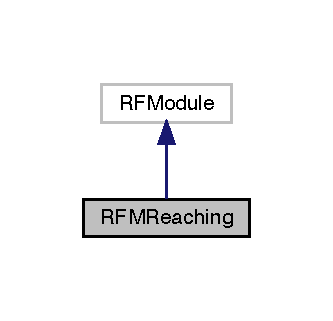
\includegraphics[width=160pt]{classRFMReaching__inherit__graph}
\end{center}
\end{figure}
\subsection*{Public Member Functions}
\begin{DoxyCompactItemize}
\item 
bool \hyperlink{classRFMReaching_a25566e4f2eed559101a37f284803f852}{configure} (Resource\+Finder \&rf)
\item 
double \hyperlink{classRFMReaching_a25880a55c1cefc2eea1718fca77a9f46}{get\+Period} ()
\item 
bool \hyperlink{classRFMReaching_a8bccf7116a170658acf11c2e0facabee}{update\+Module} ()
\item 
bool \hyperlink{classRFMReaching_a906ec163b5bfe072e988a91dca689110}{respond} (const Bottle \&command, Bottle \&reply)
\item 
bool \hyperlink{classRFMReaching_ac6343eff00e760fe31c56fa76a7e25a0}{interrupt\+Module} ()
\item 
bool \hyperlink{classRFMReaching_a96f96942041fc59fd4b5df9ecdb0fa8e}{close} ()
\end{DoxyCompactItemize}
\subsection*{Private Types}
\begin{DoxyCompactItemize}
\item 
enum \hyperlink{classRFMReaching_a45bcd979839b78397e680a4abc3443e6}{camsel} \{ \hyperlink{classRFMReaching_a45bcd979839b78397e680a4abc3443e6ad951af6aa586c134d51f4e5aee67e842}{L\+E\+FT} = 0, 
\hyperlink{classRFMReaching_a45bcd979839b78397e680a4abc3443e6a4a01bc06177ee8717dad83e5222ca7b1}{R\+I\+G\+HT} = 1
 \}
\end{DoxyCompactItemize}
\subsection*{Private Member Functions}
\begin{DoxyCompactItemize}
\item 
bool \hyperlink{classRFMReaching_a68ed451f26410a3b339d20e94cdcd3a8}{set\+Right\+Arm\+Cartesian\+Controller} ()
\item 
bool \hyperlink{classRFMReaching_a63c0db54da18c8357acfb9d55f0e7fad}{set\+Gaze\+Controller} ()
\item 
bool \hyperlink{classRFMReaching_a1898344cb04c1ae423bdaaee644b78d0}{set\+Right\+Arm\+Remote\+Controlboard} ()
\item 
bool \hyperlink{classRFMReaching_ac4f2875b315b0afc49f0e6cc4735f70f}{set\+Torso\+Remote\+Controlboard} ()
\item 
bool \hyperlink{classRFMReaching_af7908ece851513d3df2eaf75f3f45619}{set\+Torso\+D\+OF} ()
\item 
bool \hyperlink{classRFMReaching_a33ac59486a536d9334a6992d16433157}{unset\+Torso\+D\+OF} ()
\item 
Vector \hyperlink{classRFMReaching_a3a2a0c8cfdfe016a0f35cc359629f1d0}{read\+Torso} ()
\item 
Vector \hyperlink{classRFMReaching_a160dd5be2aeca203b1cffcf1ad463de7}{read\+Root\+To\+Fingers} ()
\end{DoxyCompactItemize}
\subsection*{Private Attributes}
\begin{DoxyCompactItemize}
\item 
Port \hyperlink{classRFMReaching_a916c972baaab67718ecada434ff94f98}{handler\+\_\+port\+\_\+}
\item 
bool \hyperlink{classRFMReaching_a8ca24ca1df3177f7a2086bffed644d61}{should\+\_\+stop\+\_\+} = false
\item 
S\+I\+Skeleton $\ast$ \hyperlink{classRFMReaching_aa63ad603740e3d869fc6224b7b95659b}{l\+\_\+si\+\_\+skel\+\_\+}
\item 
S\+I\+Skeleton $\ast$ \hyperlink{classRFMReaching_acbb2d80fdc4ac3222a302dfedf3aaa63}{r\+\_\+si\+\_\+skel\+\_\+}
\item 
Buffered\+Port$<$ Vector $>$ \hyperlink{classRFMReaching_a1851e362f374d6c44fedc2116a542e74}{port\+\_\+estimates\+\_\+in\+\_\+}
\item 
Buffered\+Port$<$ Image\+Of$<$ Pixel\+Rgb $>$ $>$ \hyperlink{classRFMReaching_a5972764c035d588da84616b3ca766841}{port\+\_\+image\+\_\+left\+\_\+in\+\_\+}
\item 
Buffered\+Port$<$ Image\+Of$<$ Pixel\+Rgb $>$ $>$ \hyperlink{classRFMReaching_a6a2e21f8fc0d2b96d4ac19c1c21d035f}{port\+\_\+image\+\_\+left\+\_\+out\+\_\+}
\item 
Buffered\+Port$<$ Bottle $>$ \hyperlink{classRFMReaching_ad2d1a565251ab36aab7650b1cf7840ce}{port\+\_\+click\+\_\+left\+\_\+}
\item 
Buffered\+Port$<$ Image\+Of$<$ Pixel\+Rgb $>$ $>$ \hyperlink{classRFMReaching_addc0188a22c5ab0555250721e02c6443}{port\+\_\+image\+\_\+right\+\_\+in\+\_\+}
\item 
Buffered\+Port$<$ Image\+Of$<$ Pixel\+Rgb $>$ $>$ \hyperlink{classRFMReaching_a76188810982db4710acbbb3c182f071d}{port\+\_\+image\+\_\+right\+\_\+out\+\_\+}
\item 
Buffered\+Port$<$ Bottle $>$ \hyperlink{classRFMReaching_a477a969c8c631cc7a468b0eefde2c05d}{port\+\_\+click\+\_\+right\+\_\+}
\item 
Buffered\+Port$<$ Bottle $>$ \hyperlink{classRFMReaching_ac9327dcf27ef947eb554d191362c0455}{port\+\_\+px\+\_\+left\+\_\+endeffector}
\item 
Buffered\+Port$<$ Bottle $>$ \hyperlink{classRFMReaching_a4ac92144c52def1b2990c0e7ed9f8b0d}{port\+\_\+px\+\_\+right\+\_\+endeffector}
\item 
Poly\+Driver \hyperlink{classRFMReaching_add6fb41068a3c05ebae8726873c7d73d}{rightarm\+\_\+cartesian\+\_\+driver\+\_\+}
\item 
I\+Cartesian\+Control $\ast$ \hyperlink{classRFMReaching_a5509b0b16426a661e71ae04991cd8553}{itf\+\_\+rightarm\+\_\+cart\+\_\+}
\item 
Poly\+Driver \hyperlink{classRFMReaching_ac8b09f0c704214af2cdd587b169b8240}{gaze\+\_\+driver\+\_\+}
\item 
I\+Gaze\+Control $\ast$ \hyperlink{classRFMReaching_a9d6ae2ac48ee9c5722b531c780245cf5}{itf\+\_\+gaze\+\_\+}
\item 
Poly\+Driver \hyperlink{classRFMReaching_ad7b97fed6938ffdd2e6752f5c9ae490c}{rightarm\+\_\+remote\+\_\+driver\+\_\+}
\item 
I\+Encoders $\ast$ \hyperlink{classRFMReaching_a0b9b00bc6c30770b4a12248538427864}{itf\+\_\+rightarm\+\_\+enc\+\_\+}
\item 
I\+Control\+Limits $\ast$ \hyperlink{classRFMReaching_ad99a31b38faf963ce1520f0215c3fdf3}{itf\+\_\+fingers\+\_\+lim\+\_\+}
\item 
Poly\+Driver \hyperlink{classRFMReaching_a0425996ad8eafc74f58fc8ac3db7fa85}{torso\+\_\+remote\+\_\+driver\+\_\+}
\item 
I\+Encoders $\ast$ \hyperlink{classRFMReaching_a67df5b7100117d56d535c2d4dbda72f1}{itf\+\_\+torso\+\_\+enc\+\_\+}
\item 
i\+Cub\+Finger \hyperlink{classRFMReaching_a7cc9d6f6b8bf8326e730beb1704cabc9}{icub\+\_\+index\+\_\+}
\item 
Matrix \hyperlink{classRFMReaching_a9fa03ef25eb3ad04fc6c86b642ee3e08}{left\+\_\+proj\+\_\+}
\item 
Matrix \hyperlink{classRFMReaching_a4f0aaee8537d19e7d347219d15382969}{right\+\_\+proj\+\_\+}
\item 
Matrix \hyperlink{classRFMReaching_af11a2468acda87e50de42410d80288b2}{l\+\_\+\+H\+\_\+r\+\_\+to\+\_\+cam\+\_\+}
\item 
Matrix \hyperlink{classRFMReaching_a351a3eef4730155f51d05af16b7406bf}{r\+\_\+\+H\+\_\+r\+\_\+to\+\_\+cam\+\_\+}
\item 
Matrix \hyperlink{classRFMReaching_a561ebfd0e4f966661b0c27326fec5d94}{px\+\_\+to\+\_\+cartesian\+\_\+}
\item 
double \hyperlink{classRFMReaching_ab8b1ebb26099043288c6b6da5fe7ee9b}{traj\+\_\+time\+\_\+} = 2.\+5
\item 
Vector \hyperlink{classRFMReaching_a0438d9cd07623917e3dda5eecfa34e0e}{l\+\_\+px\+\_\+goal\+\_\+}
\item 
Vector \hyperlink{classRFMReaching_a062be56961b4942fe20dd89d59abcaef}{r\+\_\+px\+\_\+goal\+\_\+}
\item 
Vector \hyperlink{classRFMReaching_a6b7de70637791218bdabe94b9613da14}{location\+\_\+}
\item 
bool \hyperlink{classRFMReaching_a28c1640ff7f4c85524567355e689ac46}{take\+\_\+estimates\+\_\+} = false
\end{DoxyCompactItemize}


\subsection{Detailed Description}


Definition at line 33 of file main.\+cpp.



\subsection{Member Enumeration Documentation}
\mbox{\Hypertarget{classRFMReaching_a45bcd979839b78397e680a4abc3443e6}\label{classRFMReaching_a45bcd979839b78397e680a4abc3443e6}} 
\index{R\+F\+M\+Reaching@{R\+F\+M\+Reaching}!camsel@{camsel}}
\index{camsel@{camsel}!R\+F\+M\+Reaching@{R\+F\+M\+Reaching}}
\subsubsection{\texorpdfstring{camsel}{camsel}}
{\footnotesize\ttfamily enum \hyperlink{classRFMReaching_a45bcd979839b78397e680a4abc3443e6}{R\+F\+M\+Reaching\+::camsel}\hspace{0.3cm}{\ttfamily [private]}}

\begin{DoxyEnumFields}{Enumerator}
\raisebox{\heightof{T}}[0pt][0pt]{\index{L\+E\+FT@{L\+E\+FT}!R\+F\+M\+Reaching@{R\+F\+M\+Reaching}}\index{R\+F\+M\+Reaching@{R\+F\+M\+Reaching}!L\+E\+FT@{L\+E\+FT}}}\mbox{\Hypertarget{classRFMReaching_a45bcd979839b78397e680a4abc3443e6ad951af6aa586c134d51f4e5aee67e842}\label{classRFMReaching_a45bcd979839b78397e680a4abc3443e6ad951af6aa586c134d51f4e5aee67e842}} 
L\+E\+FT&\\
\hline

\raisebox{\heightof{T}}[0pt][0pt]{\index{R\+I\+G\+HT@{R\+I\+G\+HT}!R\+F\+M\+Reaching@{R\+F\+M\+Reaching}}\index{R\+F\+M\+Reaching@{R\+F\+M\+Reaching}!R\+I\+G\+HT@{R\+I\+G\+HT}}}\mbox{\Hypertarget{classRFMReaching_a45bcd979839b78397e680a4abc3443e6a4a01bc06177ee8717dad83e5222ca7b1}\label{classRFMReaching_a45bcd979839b78397e680a4abc3443e6a4a01bc06177ee8717dad83e5222ca7b1}} 
R\+I\+G\+HT&\\
\hline

\end{DoxyEnumFields}


Definition at line 1005 of file main.\+cpp.



\subsection{Member Function Documentation}
\mbox{\Hypertarget{classRFMReaching_a96f96942041fc59fd4b5df9ecdb0fa8e}\label{classRFMReaching_a96f96942041fc59fd4b5df9ecdb0fa8e}} 
\index{R\+F\+M\+Reaching@{R\+F\+M\+Reaching}!close@{close}}
\index{close@{close}!R\+F\+M\+Reaching@{R\+F\+M\+Reaching}}
\subsubsection{\texorpdfstring{close()}{close()}}
{\footnotesize\ttfamily bool R\+F\+M\+Reaching\+::close (\begin{DoxyParamCaption}{ }\end{DoxyParamCaption})\hspace{0.3cm}{\ttfamily [inline]}}



Definition at line 936 of file main.\+cpp.

\mbox{\Hypertarget{classRFMReaching_a25566e4f2eed559101a37f284803f852}\label{classRFMReaching_a25566e4f2eed559101a37f284803f852}} 
\index{R\+F\+M\+Reaching@{R\+F\+M\+Reaching}!configure@{configure}}
\index{configure@{configure}!R\+F\+M\+Reaching@{R\+F\+M\+Reaching}}
\subsubsection{\texorpdfstring{configure()}{configure()}}
{\footnotesize\ttfamily bool R\+F\+M\+Reaching\+::configure (\begin{DoxyParamCaption}\item[{Resource\+Finder \&}]{rf }\end{DoxyParamCaption})\hspace{0.3cm}{\ttfamily [inline]}}



Definition at line 36 of file main.\+cpp.

\mbox{\Hypertarget{classRFMReaching_a25880a55c1cefc2eea1718fca77a9f46}\label{classRFMReaching_a25880a55c1cefc2eea1718fca77a9f46}} 
\index{R\+F\+M\+Reaching@{R\+F\+M\+Reaching}!get\+Period@{get\+Period}}
\index{get\+Period@{get\+Period}!R\+F\+M\+Reaching@{R\+F\+M\+Reaching}}
\subsubsection{\texorpdfstring{get\+Period()}{getPeriod()}}
{\footnotesize\ttfamily double R\+F\+M\+Reaching\+::get\+Period (\begin{DoxyParamCaption}{ }\end{DoxyParamCaption})\hspace{0.3cm}{\ttfamily [inline]}}



Definition at line 186 of file main.\+cpp.

\mbox{\Hypertarget{classRFMReaching_ac6343eff00e760fe31c56fa76a7e25a0}\label{classRFMReaching_ac6343eff00e760fe31c56fa76a7e25a0}} 
\index{R\+F\+M\+Reaching@{R\+F\+M\+Reaching}!interrupt\+Module@{interrupt\+Module}}
\index{interrupt\+Module@{interrupt\+Module}!R\+F\+M\+Reaching@{R\+F\+M\+Reaching}}
\subsubsection{\texorpdfstring{interrupt\+Module()}{interruptModule()}}
{\footnotesize\ttfamily bool R\+F\+M\+Reaching\+::interrupt\+Module (\begin{DoxyParamCaption}{ }\end{DoxyParamCaption})\hspace{0.3cm}{\ttfamily [inline]}}



Definition at line 918 of file main.\+cpp.

\mbox{\Hypertarget{classRFMReaching_a160dd5be2aeca203b1cffcf1ad463de7}\label{classRFMReaching_a160dd5be2aeca203b1cffcf1ad463de7}} 
\index{R\+F\+M\+Reaching@{R\+F\+M\+Reaching}!read\+Root\+To\+Fingers@{read\+Root\+To\+Fingers}}
\index{read\+Root\+To\+Fingers@{read\+Root\+To\+Fingers}!R\+F\+M\+Reaching@{R\+F\+M\+Reaching}}
\subsubsection{\texorpdfstring{read\+Root\+To\+Fingers()}{readRootToFingers()}}
{\footnotesize\ttfamily Vector R\+F\+M\+Reaching\+::read\+Root\+To\+Fingers (\begin{DoxyParamCaption}{ }\end{DoxyParamCaption})\hspace{0.3cm}{\ttfamily [inline]}, {\ttfamily [private]}}



Definition at line 1193 of file main.\+cpp.

\mbox{\Hypertarget{classRFMReaching_a3a2a0c8cfdfe016a0f35cc359629f1d0}\label{classRFMReaching_a3a2a0c8cfdfe016a0f35cc359629f1d0}} 
\index{R\+F\+M\+Reaching@{R\+F\+M\+Reaching}!read\+Torso@{read\+Torso}}
\index{read\+Torso@{read\+Torso}!R\+F\+M\+Reaching@{R\+F\+M\+Reaching}}
\subsubsection{\texorpdfstring{read\+Torso()}{readTorso()}}
{\footnotesize\ttfamily Vector R\+F\+M\+Reaching\+::read\+Torso (\begin{DoxyParamCaption}{ }\end{DoxyParamCaption})\hspace{0.3cm}{\ttfamily [inline]}, {\ttfamily [private]}}



Definition at line 1183 of file main.\+cpp.

\mbox{\Hypertarget{classRFMReaching_a906ec163b5bfe072e988a91dca689110}\label{classRFMReaching_a906ec163b5bfe072e988a91dca689110}} 
\index{R\+F\+M\+Reaching@{R\+F\+M\+Reaching}!respond@{respond}}
\index{respond@{respond}!R\+F\+M\+Reaching@{R\+F\+M\+Reaching}}
\subsubsection{\texorpdfstring{respond()}{respond()}}
{\footnotesize\ttfamily bool R\+F\+M\+Reaching\+::respond (\begin{DoxyParamCaption}\item[{const Bottle \&}]{command,  }\item[{Bottle \&}]{reply }\end{DoxyParamCaption})\hspace{0.3cm}{\ttfamily [inline]}}



Definition at line 486 of file main.\+cpp.

\mbox{\Hypertarget{classRFMReaching_a63c0db54da18c8357acfb9d55f0e7fad}\label{classRFMReaching_a63c0db54da18c8357acfb9d55f0e7fad}} 
\index{R\+F\+M\+Reaching@{R\+F\+M\+Reaching}!set\+Gaze\+Controller@{set\+Gaze\+Controller}}
\index{set\+Gaze\+Controller@{set\+Gaze\+Controller}!R\+F\+M\+Reaching@{R\+F\+M\+Reaching}}
\subsubsection{\texorpdfstring{set\+Gaze\+Controller()}{setGazeController()}}
{\footnotesize\ttfamily bool R\+F\+M\+Reaching\+::set\+Gaze\+Controller (\begin{DoxyParamCaption}{ }\end{DoxyParamCaption})\hspace{0.3cm}{\ttfamily [inline]}, {\ttfamily [private]}}



Definition at line 1052 of file main.\+cpp.

\mbox{\Hypertarget{classRFMReaching_a68ed451f26410a3b339d20e94cdcd3a8}\label{classRFMReaching_a68ed451f26410a3b339d20e94cdcd3a8}} 
\index{R\+F\+M\+Reaching@{R\+F\+M\+Reaching}!set\+Right\+Arm\+Cartesian\+Controller@{set\+Right\+Arm\+Cartesian\+Controller}}
\index{set\+Right\+Arm\+Cartesian\+Controller@{set\+Right\+Arm\+Cartesian\+Controller}!R\+F\+M\+Reaching@{R\+F\+M\+Reaching}}
\subsubsection{\texorpdfstring{set\+Right\+Arm\+Cartesian\+Controller()}{setRightArmCartesianController()}}
{\footnotesize\ttfamily bool R\+F\+M\+Reaching\+::set\+Right\+Arm\+Cartesian\+Controller (\begin{DoxyParamCaption}{ }\end{DoxyParamCaption})\hspace{0.3cm}{\ttfamily [inline]}, {\ttfamily [private]}}



Definition at line 1011 of file main.\+cpp.

\mbox{\Hypertarget{classRFMReaching_a1898344cb04c1ae423bdaaee644b78d0}\label{classRFMReaching_a1898344cb04c1ae423bdaaee644b78d0}} 
\index{R\+F\+M\+Reaching@{R\+F\+M\+Reaching}!set\+Right\+Arm\+Remote\+Controlboard@{set\+Right\+Arm\+Remote\+Controlboard}}
\index{set\+Right\+Arm\+Remote\+Controlboard@{set\+Right\+Arm\+Remote\+Controlboard}!R\+F\+M\+Reaching@{R\+F\+M\+Reaching}}
\subsubsection{\texorpdfstring{set\+Right\+Arm\+Remote\+Controlboard()}{setRightArmRemoteControlboard()}}
{\footnotesize\ttfamily bool R\+F\+M\+Reaching\+::set\+Right\+Arm\+Remote\+Controlboard (\begin{DoxyParamCaption}{ }\end{DoxyParamCaption})\hspace{0.3cm}{\ttfamily [inline]}, {\ttfamily [private]}}



Definition at line 1078 of file main.\+cpp.

\mbox{\Hypertarget{classRFMReaching_af7908ece851513d3df2eaf75f3f45619}\label{classRFMReaching_af7908ece851513d3df2eaf75f3f45619}} 
\index{R\+F\+M\+Reaching@{R\+F\+M\+Reaching}!set\+Torso\+D\+OF@{set\+Torso\+D\+OF}}
\index{set\+Torso\+D\+OF@{set\+Torso\+D\+OF}!R\+F\+M\+Reaching@{R\+F\+M\+Reaching}}
\subsubsection{\texorpdfstring{set\+Torso\+D\+O\+F()}{setTorsoDOF()}}
{\footnotesize\ttfamily bool R\+F\+M\+Reaching\+::set\+Torso\+D\+OF (\begin{DoxyParamCaption}{ }\end{DoxyParamCaption})\hspace{0.3cm}{\ttfamily [inline]}, {\ttfamily [private]}}



Definition at line 1141 of file main.\+cpp.

\mbox{\Hypertarget{classRFMReaching_ac4f2875b315b0afc49f0e6cc4735f70f}\label{classRFMReaching_ac4f2875b315b0afc49f0e6cc4735f70f}} 
\index{R\+F\+M\+Reaching@{R\+F\+M\+Reaching}!set\+Torso\+Remote\+Controlboard@{set\+Torso\+Remote\+Controlboard}}
\index{set\+Torso\+Remote\+Controlboard@{set\+Torso\+Remote\+Controlboard}!R\+F\+M\+Reaching@{R\+F\+M\+Reaching}}
\subsubsection{\texorpdfstring{set\+Torso\+Remote\+Controlboard()}{setTorsoRemoteControlboard()}}
{\footnotesize\ttfamily bool R\+F\+M\+Reaching\+::set\+Torso\+Remote\+Controlboard (\begin{DoxyParamCaption}{ }\end{DoxyParamCaption})\hspace{0.3cm}{\ttfamily [inline]}, {\ttfamily [private]}}



Definition at line 1113 of file main.\+cpp.

\mbox{\Hypertarget{classRFMReaching_a33ac59486a536d9334a6992d16433157}\label{classRFMReaching_a33ac59486a536d9334a6992d16433157}} 
\index{R\+F\+M\+Reaching@{R\+F\+M\+Reaching}!unset\+Torso\+D\+OF@{unset\+Torso\+D\+OF}}
\index{unset\+Torso\+D\+OF@{unset\+Torso\+D\+OF}!R\+F\+M\+Reaching@{R\+F\+M\+Reaching}}
\subsubsection{\texorpdfstring{unset\+Torso\+D\+O\+F()}{unsetTorsoDOF()}}
{\footnotesize\ttfamily bool R\+F\+M\+Reaching\+::unset\+Torso\+D\+OF (\begin{DoxyParamCaption}{ }\end{DoxyParamCaption})\hspace{0.3cm}{\ttfamily [inline]}, {\ttfamily [private]}}



Definition at line 1162 of file main.\+cpp.

\mbox{\Hypertarget{classRFMReaching_a8bccf7116a170658acf11c2e0facabee}\label{classRFMReaching_a8bccf7116a170658acf11c2e0facabee}} 
\index{R\+F\+M\+Reaching@{R\+F\+M\+Reaching}!update\+Module@{update\+Module}}
\index{update\+Module@{update\+Module}!R\+F\+M\+Reaching@{R\+F\+M\+Reaching}}
\subsubsection{\texorpdfstring{update\+Module()}{updateModule()}}
{\footnotesize\ttfamily bool R\+F\+M\+Reaching\+::update\+Module (\begin{DoxyParamCaption}{ }\end{DoxyParamCaption})\hspace{0.3cm}{\ttfamily [inline]}}



Definition at line 189 of file main.\+cpp.



\subsection{Member Data Documentation}
\mbox{\Hypertarget{classRFMReaching_ac8b09f0c704214af2cdd587b169b8240}\label{classRFMReaching_ac8b09f0c704214af2cdd587b169b8240}} 
\index{R\+F\+M\+Reaching@{R\+F\+M\+Reaching}!gaze\+\_\+driver\+\_\+@{gaze\+\_\+driver\+\_\+}}
\index{gaze\+\_\+driver\+\_\+@{gaze\+\_\+driver\+\_\+}!R\+F\+M\+Reaching@{R\+F\+M\+Reaching}}
\subsubsection{\texorpdfstring{gaze\+\_\+driver\+\_\+}{gaze\_driver\_}}
{\footnotesize\ttfamily Poly\+Driver R\+F\+M\+Reaching\+::gaze\+\_\+driver\+\_\+\hspace{0.3cm}{\ttfamily [private]}}



Definition at line 981 of file main.\+cpp.

\mbox{\Hypertarget{classRFMReaching_a916c972baaab67718ecada434ff94f98}\label{classRFMReaching_a916c972baaab67718ecada434ff94f98}} 
\index{R\+F\+M\+Reaching@{R\+F\+M\+Reaching}!handler\+\_\+port\+\_\+@{handler\+\_\+port\+\_\+}}
\index{handler\+\_\+port\+\_\+@{handler\+\_\+port\+\_\+}!R\+F\+M\+Reaching@{R\+F\+M\+Reaching}}
\subsubsection{\texorpdfstring{handler\+\_\+port\+\_\+}{handler\_port\_}}
{\footnotesize\ttfamily Port R\+F\+M\+Reaching\+::handler\+\_\+port\+\_\+\hspace{0.3cm}{\ttfamily [private]}}



Definition at line 959 of file main.\+cpp.

\mbox{\Hypertarget{classRFMReaching_a7cc9d6f6b8bf8326e730beb1704cabc9}\label{classRFMReaching_a7cc9d6f6b8bf8326e730beb1704cabc9}} 
\index{R\+F\+M\+Reaching@{R\+F\+M\+Reaching}!icub\+\_\+index\+\_\+@{icub\+\_\+index\+\_\+}}
\index{icub\+\_\+index\+\_\+@{icub\+\_\+index\+\_\+}!R\+F\+M\+Reaching@{R\+F\+M\+Reaching}}
\subsubsection{\texorpdfstring{icub\+\_\+index\+\_\+}{icub\_index\_}}
{\footnotesize\ttfamily i\+Cub\+Finger R\+F\+M\+Reaching\+::icub\+\_\+index\+\_\+\hspace{0.3cm}{\ttfamily [private]}}



Definition at line 991 of file main.\+cpp.

\mbox{\Hypertarget{classRFMReaching_ad99a31b38faf963ce1520f0215c3fdf3}\label{classRFMReaching_ad99a31b38faf963ce1520f0215c3fdf3}} 
\index{R\+F\+M\+Reaching@{R\+F\+M\+Reaching}!itf\+\_\+fingers\+\_\+lim\+\_\+@{itf\+\_\+fingers\+\_\+lim\+\_\+}}
\index{itf\+\_\+fingers\+\_\+lim\+\_\+@{itf\+\_\+fingers\+\_\+lim\+\_\+}!R\+F\+M\+Reaching@{R\+F\+M\+Reaching}}
\subsubsection{\texorpdfstring{itf\+\_\+fingers\+\_\+lim\+\_\+}{itf\_fingers\_lim\_}}
{\footnotesize\ttfamily I\+Control\+Limits$\ast$ R\+F\+M\+Reaching\+::itf\+\_\+fingers\+\_\+lim\+\_\+\hspace{0.3cm}{\ttfamily [private]}}



Definition at line 986 of file main.\+cpp.

\mbox{\Hypertarget{classRFMReaching_a9d6ae2ac48ee9c5722b531c780245cf5}\label{classRFMReaching_a9d6ae2ac48ee9c5722b531c780245cf5}} 
\index{R\+F\+M\+Reaching@{R\+F\+M\+Reaching}!itf\+\_\+gaze\+\_\+@{itf\+\_\+gaze\+\_\+}}
\index{itf\+\_\+gaze\+\_\+@{itf\+\_\+gaze\+\_\+}!R\+F\+M\+Reaching@{R\+F\+M\+Reaching}}
\subsubsection{\texorpdfstring{itf\+\_\+gaze\+\_\+}{itf\_gaze\_}}
{\footnotesize\ttfamily I\+Gaze\+Control$\ast$ R\+F\+M\+Reaching\+::itf\+\_\+gaze\+\_\+\hspace{0.3cm}{\ttfamily [private]}}



Definition at line 982 of file main.\+cpp.

\mbox{\Hypertarget{classRFMReaching_a5509b0b16426a661e71ae04991cd8553}\label{classRFMReaching_a5509b0b16426a661e71ae04991cd8553}} 
\index{R\+F\+M\+Reaching@{R\+F\+M\+Reaching}!itf\+\_\+rightarm\+\_\+cart\+\_\+@{itf\+\_\+rightarm\+\_\+cart\+\_\+}}
\index{itf\+\_\+rightarm\+\_\+cart\+\_\+@{itf\+\_\+rightarm\+\_\+cart\+\_\+}!R\+F\+M\+Reaching@{R\+F\+M\+Reaching}}
\subsubsection{\texorpdfstring{itf\+\_\+rightarm\+\_\+cart\+\_\+}{itf\_rightarm\_cart\_}}
{\footnotesize\ttfamily I\+Cartesian\+Control$\ast$ R\+F\+M\+Reaching\+::itf\+\_\+rightarm\+\_\+cart\+\_\+\hspace{0.3cm}{\ttfamily [private]}}



Definition at line 979 of file main.\+cpp.

\mbox{\Hypertarget{classRFMReaching_a0b9b00bc6c30770b4a12248538427864}\label{classRFMReaching_a0b9b00bc6c30770b4a12248538427864}} 
\index{R\+F\+M\+Reaching@{R\+F\+M\+Reaching}!itf\+\_\+rightarm\+\_\+enc\+\_\+@{itf\+\_\+rightarm\+\_\+enc\+\_\+}}
\index{itf\+\_\+rightarm\+\_\+enc\+\_\+@{itf\+\_\+rightarm\+\_\+enc\+\_\+}!R\+F\+M\+Reaching@{R\+F\+M\+Reaching}}
\subsubsection{\texorpdfstring{itf\+\_\+rightarm\+\_\+enc\+\_\+}{itf\_rightarm\_enc\_}}
{\footnotesize\ttfamily I\+Encoders$\ast$ R\+F\+M\+Reaching\+::itf\+\_\+rightarm\+\_\+enc\+\_\+\hspace{0.3cm}{\ttfamily [private]}}



Definition at line 985 of file main.\+cpp.

\mbox{\Hypertarget{classRFMReaching_a67df5b7100117d56d535c2d4dbda72f1}\label{classRFMReaching_a67df5b7100117d56d535c2d4dbda72f1}} 
\index{R\+F\+M\+Reaching@{R\+F\+M\+Reaching}!itf\+\_\+torso\+\_\+enc\+\_\+@{itf\+\_\+torso\+\_\+enc\+\_\+}}
\index{itf\+\_\+torso\+\_\+enc\+\_\+@{itf\+\_\+torso\+\_\+enc\+\_\+}!R\+F\+M\+Reaching@{R\+F\+M\+Reaching}}
\subsubsection{\texorpdfstring{itf\+\_\+torso\+\_\+enc\+\_\+}{itf\_torso\_enc\_}}
{\footnotesize\ttfamily I\+Encoders$\ast$ R\+F\+M\+Reaching\+::itf\+\_\+torso\+\_\+enc\+\_\+\hspace{0.3cm}{\ttfamily [private]}}



Definition at line 989 of file main.\+cpp.

\mbox{\Hypertarget{classRFMReaching_af11a2468acda87e50de42410d80288b2}\label{classRFMReaching_af11a2468acda87e50de42410d80288b2}} 
\index{R\+F\+M\+Reaching@{R\+F\+M\+Reaching}!l\+\_\+\+H\+\_\+r\+\_\+to\+\_\+cam\+\_\+@{l\+\_\+\+H\+\_\+r\+\_\+to\+\_\+cam\+\_\+}}
\index{l\+\_\+\+H\+\_\+r\+\_\+to\+\_\+cam\+\_\+@{l\+\_\+\+H\+\_\+r\+\_\+to\+\_\+cam\+\_\+}!R\+F\+M\+Reaching@{R\+F\+M\+Reaching}}
\subsubsection{\texorpdfstring{l\+\_\+\+H\+\_\+r\+\_\+to\+\_\+cam\+\_\+}{l\_H\_r\_to\_cam\_}}
{\footnotesize\ttfamily Matrix R\+F\+M\+Reaching\+::l\+\_\+\+H\+\_\+r\+\_\+to\+\_\+cam\+\_\+\hspace{0.3cm}{\ttfamily [private]}}



Definition at line 995 of file main.\+cpp.

\mbox{\Hypertarget{classRFMReaching_a0438d9cd07623917e3dda5eecfa34e0e}\label{classRFMReaching_a0438d9cd07623917e3dda5eecfa34e0e}} 
\index{R\+F\+M\+Reaching@{R\+F\+M\+Reaching}!l\+\_\+px\+\_\+goal\+\_\+@{l\+\_\+px\+\_\+goal\+\_\+}}
\index{l\+\_\+px\+\_\+goal\+\_\+@{l\+\_\+px\+\_\+goal\+\_\+}!R\+F\+M\+Reaching@{R\+F\+M\+Reaching}}
\subsubsection{\texorpdfstring{l\+\_\+px\+\_\+goal\+\_\+}{l\_px\_goal\_}}
{\footnotesize\ttfamily Vector R\+F\+M\+Reaching\+::l\+\_\+px\+\_\+goal\+\_\+\hspace{0.3cm}{\ttfamily [private]}}



Definition at line 1000 of file main.\+cpp.

\mbox{\Hypertarget{classRFMReaching_aa63ad603740e3d869fc6224b7b95659b}\label{classRFMReaching_aa63ad603740e3d869fc6224b7b95659b}} 
\index{R\+F\+M\+Reaching@{R\+F\+M\+Reaching}!l\+\_\+si\+\_\+skel\+\_\+@{l\+\_\+si\+\_\+skel\+\_\+}}
\index{l\+\_\+si\+\_\+skel\+\_\+@{l\+\_\+si\+\_\+skel\+\_\+}!R\+F\+M\+Reaching@{R\+F\+M\+Reaching}}
\subsubsection{\texorpdfstring{l\+\_\+si\+\_\+skel\+\_\+}{l\_si\_skel\_}}
{\footnotesize\ttfamily S\+I\+Skeleton$\ast$ R\+F\+M\+Reaching\+::l\+\_\+si\+\_\+skel\+\_\+\hspace{0.3cm}{\ttfamily [private]}}



Definition at line 962 of file main.\+cpp.

\mbox{\Hypertarget{classRFMReaching_a9fa03ef25eb3ad04fc6c86b642ee3e08}\label{classRFMReaching_a9fa03ef25eb3ad04fc6c86b642ee3e08}} 
\index{R\+F\+M\+Reaching@{R\+F\+M\+Reaching}!left\+\_\+proj\+\_\+@{left\+\_\+proj\+\_\+}}
\index{left\+\_\+proj\+\_\+@{left\+\_\+proj\+\_\+}!R\+F\+M\+Reaching@{R\+F\+M\+Reaching}}
\subsubsection{\texorpdfstring{left\+\_\+proj\+\_\+}{left\_proj\_}}
{\footnotesize\ttfamily Matrix R\+F\+M\+Reaching\+::left\+\_\+proj\+\_\+\hspace{0.3cm}{\ttfamily [private]}}



Definition at line 993 of file main.\+cpp.

\mbox{\Hypertarget{classRFMReaching_a6b7de70637791218bdabe94b9613da14}\label{classRFMReaching_a6b7de70637791218bdabe94b9613da14}} 
\index{R\+F\+M\+Reaching@{R\+F\+M\+Reaching}!location\+\_\+@{location\+\_\+}}
\index{location\+\_\+@{location\+\_\+}!R\+F\+M\+Reaching@{R\+F\+M\+Reaching}}
\subsubsection{\texorpdfstring{location\+\_\+}{location\_}}
{\footnotesize\ttfamily Vector R\+F\+M\+Reaching\+::location\+\_\+\hspace{0.3cm}{\ttfamily [private]}}



Definition at line 1002 of file main.\+cpp.

\mbox{\Hypertarget{classRFMReaching_ad2d1a565251ab36aab7650b1cf7840ce}\label{classRFMReaching_ad2d1a565251ab36aab7650b1cf7840ce}} 
\index{R\+F\+M\+Reaching@{R\+F\+M\+Reaching}!port\+\_\+click\+\_\+left\+\_\+@{port\+\_\+click\+\_\+left\+\_\+}}
\index{port\+\_\+click\+\_\+left\+\_\+@{port\+\_\+click\+\_\+left\+\_\+}!R\+F\+M\+Reaching@{R\+F\+M\+Reaching}}
\subsubsection{\texorpdfstring{port\+\_\+click\+\_\+left\+\_\+}{port\_click\_left\_}}
{\footnotesize\ttfamily Buffered\+Port$<$Bottle$>$ R\+F\+M\+Reaching\+::port\+\_\+click\+\_\+left\+\_\+\hspace{0.3cm}{\ttfamily [private]}}



Definition at line 969 of file main.\+cpp.

\mbox{\Hypertarget{classRFMReaching_a477a969c8c631cc7a468b0eefde2c05d}\label{classRFMReaching_a477a969c8c631cc7a468b0eefde2c05d}} 
\index{R\+F\+M\+Reaching@{R\+F\+M\+Reaching}!port\+\_\+click\+\_\+right\+\_\+@{port\+\_\+click\+\_\+right\+\_\+}}
\index{port\+\_\+click\+\_\+right\+\_\+@{port\+\_\+click\+\_\+right\+\_\+}!R\+F\+M\+Reaching@{R\+F\+M\+Reaching}}
\subsubsection{\texorpdfstring{port\+\_\+click\+\_\+right\+\_\+}{port\_click\_right\_}}
{\footnotesize\ttfamily Buffered\+Port$<$Bottle$>$ R\+F\+M\+Reaching\+::port\+\_\+click\+\_\+right\+\_\+\hspace{0.3cm}{\ttfamily [private]}}



Definition at line 973 of file main.\+cpp.

\mbox{\Hypertarget{classRFMReaching_a1851e362f374d6c44fedc2116a542e74}\label{classRFMReaching_a1851e362f374d6c44fedc2116a542e74}} 
\index{R\+F\+M\+Reaching@{R\+F\+M\+Reaching}!port\+\_\+estimates\+\_\+in\+\_\+@{port\+\_\+estimates\+\_\+in\+\_\+}}
\index{port\+\_\+estimates\+\_\+in\+\_\+@{port\+\_\+estimates\+\_\+in\+\_\+}!R\+F\+M\+Reaching@{R\+F\+M\+Reaching}}
\subsubsection{\texorpdfstring{port\+\_\+estimates\+\_\+in\+\_\+}{port\_estimates\_in\_}}
{\footnotesize\ttfamily Buffered\+Port$<$Vector$>$ R\+F\+M\+Reaching\+::port\+\_\+estimates\+\_\+in\+\_\+\hspace{0.3cm}{\ttfamily [private]}}



Definition at line 965 of file main.\+cpp.

\mbox{\Hypertarget{classRFMReaching_a5972764c035d588da84616b3ca766841}\label{classRFMReaching_a5972764c035d588da84616b3ca766841}} 
\index{R\+F\+M\+Reaching@{R\+F\+M\+Reaching}!port\+\_\+image\+\_\+left\+\_\+in\+\_\+@{port\+\_\+image\+\_\+left\+\_\+in\+\_\+}}
\index{port\+\_\+image\+\_\+left\+\_\+in\+\_\+@{port\+\_\+image\+\_\+left\+\_\+in\+\_\+}!R\+F\+M\+Reaching@{R\+F\+M\+Reaching}}
\subsubsection{\texorpdfstring{port\+\_\+image\+\_\+left\+\_\+in\+\_\+}{port\_image\_left\_in\_}}
{\footnotesize\ttfamily Buffered\+Port$<$Image\+Of$<$Pixel\+Rgb$>$ $>$ R\+F\+M\+Reaching\+::port\+\_\+image\+\_\+left\+\_\+in\+\_\+\hspace{0.3cm}{\ttfamily [private]}}



Definition at line 967 of file main.\+cpp.

\mbox{\Hypertarget{classRFMReaching_a6a2e21f8fc0d2b96d4ac19c1c21d035f}\label{classRFMReaching_a6a2e21f8fc0d2b96d4ac19c1c21d035f}} 
\index{R\+F\+M\+Reaching@{R\+F\+M\+Reaching}!port\+\_\+image\+\_\+left\+\_\+out\+\_\+@{port\+\_\+image\+\_\+left\+\_\+out\+\_\+}}
\index{port\+\_\+image\+\_\+left\+\_\+out\+\_\+@{port\+\_\+image\+\_\+left\+\_\+out\+\_\+}!R\+F\+M\+Reaching@{R\+F\+M\+Reaching}}
\subsubsection{\texorpdfstring{port\+\_\+image\+\_\+left\+\_\+out\+\_\+}{port\_image\_left\_out\_}}
{\footnotesize\ttfamily Buffered\+Port$<$Image\+Of$<$Pixel\+Rgb$>$ $>$ R\+F\+M\+Reaching\+::port\+\_\+image\+\_\+left\+\_\+out\+\_\+\hspace{0.3cm}{\ttfamily [private]}}



Definition at line 968 of file main.\+cpp.

\mbox{\Hypertarget{classRFMReaching_addc0188a22c5ab0555250721e02c6443}\label{classRFMReaching_addc0188a22c5ab0555250721e02c6443}} 
\index{R\+F\+M\+Reaching@{R\+F\+M\+Reaching}!port\+\_\+image\+\_\+right\+\_\+in\+\_\+@{port\+\_\+image\+\_\+right\+\_\+in\+\_\+}}
\index{port\+\_\+image\+\_\+right\+\_\+in\+\_\+@{port\+\_\+image\+\_\+right\+\_\+in\+\_\+}!R\+F\+M\+Reaching@{R\+F\+M\+Reaching}}
\subsubsection{\texorpdfstring{port\+\_\+image\+\_\+right\+\_\+in\+\_\+}{port\_image\_right\_in\_}}
{\footnotesize\ttfamily Buffered\+Port$<$Image\+Of$<$Pixel\+Rgb$>$ $>$ R\+F\+M\+Reaching\+::port\+\_\+image\+\_\+right\+\_\+in\+\_\+\hspace{0.3cm}{\ttfamily [private]}}



Definition at line 971 of file main.\+cpp.

\mbox{\Hypertarget{classRFMReaching_a76188810982db4710acbbb3c182f071d}\label{classRFMReaching_a76188810982db4710acbbb3c182f071d}} 
\index{R\+F\+M\+Reaching@{R\+F\+M\+Reaching}!port\+\_\+image\+\_\+right\+\_\+out\+\_\+@{port\+\_\+image\+\_\+right\+\_\+out\+\_\+}}
\index{port\+\_\+image\+\_\+right\+\_\+out\+\_\+@{port\+\_\+image\+\_\+right\+\_\+out\+\_\+}!R\+F\+M\+Reaching@{R\+F\+M\+Reaching}}
\subsubsection{\texorpdfstring{port\+\_\+image\+\_\+right\+\_\+out\+\_\+}{port\_image\_right\_out\_}}
{\footnotesize\ttfamily Buffered\+Port$<$Image\+Of$<$Pixel\+Rgb$>$ $>$ R\+F\+M\+Reaching\+::port\+\_\+image\+\_\+right\+\_\+out\+\_\+\hspace{0.3cm}{\ttfamily [private]}}



Definition at line 972 of file main.\+cpp.

\mbox{\Hypertarget{classRFMReaching_ac9327dcf27ef947eb554d191362c0455}\label{classRFMReaching_ac9327dcf27ef947eb554d191362c0455}} 
\index{R\+F\+M\+Reaching@{R\+F\+M\+Reaching}!port\+\_\+px\+\_\+left\+\_\+endeffector@{port\+\_\+px\+\_\+left\+\_\+endeffector}}
\index{port\+\_\+px\+\_\+left\+\_\+endeffector@{port\+\_\+px\+\_\+left\+\_\+endeffector}!R\+F\+M\+Reaching@{R\+F\+M\+Reaching}}
\subsubsection{\texorpdfstring{port\+\_\+px\+\_\+left\+\_\+endeffector}{port\_px\_left\_endeffector}}
{\footnotesize\ttfamily Buffered\+Port$<$Bottle$>$ R\+F\+M\+Reaching\+::port\+\_\+px\+\_\+left\+\_\+endeffector\hspace{0.3cm}{\ttfamily [private]}}



Definition at line 975 of file main.\+cpp.

\mbox{\Hypertarget{classRFMReaching_a4ac92144c52def1b2990c0e7ed9f8b0d}\label{classRFMReaching_a4ac92144c52def1b2990c0e7ed9f8b0d}} 
\index{R\+F\+M\+Reaching@{R\+F\+M\+Reaching}!port\+\_\+px\+\_\+right\+\_\+endeffector@{port\+\_\+px\+\_\+right\+\_\+endeffector}}
\index{port\+\_\+px\+\_\+right\+\_\+endeffector@{port\+\_\+px\+\_\+right\+\_\+endeffector}!R\+F\+M\+Reaching@{R\+F\+M\+Reaching}}
\subsubsection{\texorpdfstring{port\+\_\+px\+\_\+right\+\_\+endeffector}{port\_px\_right\_endeffector}}
{\footnotesize\ttfamily Buffered\+Port$<$Bottle$>$ R\+F\+M\+Reaching\+::port\+\_\+px\+\_\+right\+\_\+endeffector\hspace{0.3cm}{\ttfamily [private]}}



Definition at line 976 of file main.\+cpp.

\mbox{\Hypertarget{classRFMReaching_a561ebfd0e4f966661b0c27326fec5d94}\label{classRFMReaching_a561ebfd0e4f966661b0c27326fec5d94}} 
\index{R\+F\+M\+Reaching@{R\+F\+M\+Reaching}!px\+\_\+to\+\_\+cartesian\+\_\+@{px\+\_\+to\+\_\+cartesian\+\_\+}}
\index{px\+\_\+to\+\_\+cartesian\+\_\+@{px\+\_\+to\+\_\+cartesian\+\_\+}!R\+F\+M\+Reaching@{R\+F\+M\+Reaching}}
\subsubsection{\texorpdfstring{px\+\_\+to\+\_\+cartesian\+\_\+}{px\_to\_cartesian\_}}
{\footnotesize\ttfamily Matrix R\+F\+M\+Reaching\+::px\+\_\+to\+\_\+cartesian\+\_\+\hspace{0.3cm}{\ttfamily [private]}}



Definition at line 997 of file main.\+cpp.

\mbox{\Hypertarget{classRFMReaching_a351a3eef4730155f51d05af16b7406bf}\label{classRFMReaching_a351a3eef4730155f51d05af16b7406bf}} 
\index{R\+F\+M\+Reaching@{R\+F\+M\+Reaching}!r\+\_\+\+H\+\_\+r\+\_\+to\+\_\+cam\+\_\+@{r\+\_\+\+H\+\_\+r\+\_\+to\+\_\+cam\+\_\+}}
\index{r\+\_\+\+H\+\_\+r\+\_\+to\+\_\+cam\+\_\+@{r\+\_\+\+H\+\_\+r\+\_\+to\+\_\+cam\+\_\+}!R\+F\+M\+Reaching@{R\+F\+M\+Reaching}}
\subsubsection{\texorpdfstring{r\+\_\+\+H\+\_\+r\+\_\+to\+\_\+cam\+\_\+}{r\_H\_r\_to\_cam\_}}
{\footnotesize\ttfamily Matrix R\+F\+M\+Reaching\+::r\+\_\+\+H\+\_\+r\+\_\+to\+\_\+cam\+\_\+\hspace{0.3cm}{\ttfamily [private]}}



Definition at line 996 of file main.\+cpp.

\mbox{\Hypertarget{classRFMReaching_a062be56961b4942fe20dd89d59abcaef}\label{classRFMReaching_a062be56961b4942fe20dd89d59abcaef}} 
\index{R\+F\+M\+Reaching@{R\+F\+M\+Reaching}!r\+\_\+px\+\_\+goal\+\_\+@{r\+\_\+px\+\_\+goal\+\_\+}}
\index{r\+\_\+px\+\_\+goal\+\_\+@{r\+\_\+px\+\_\+goal\+\_\+}!R\+F\+M\+Reaching@{R\+F\+M\+Reaching}}
\subsubsection{\texorpdfstring{r\+\_\+px\+\_\+goal\+\_\+}{r\_px\_goal\_}}
{\footnotesize\ttfamily Vector R\+F\+M\+Reaching\+::r\+\_\+px\+\_\+goal\+\_\+\hspace{0.3cm}{\ttfamily [private]}}



Definition at line 1001 of file main.\+cpp.

\mbox{\Hypertarget{classRFMReaching_acbb2d80fdc4ac3222a302dfedf3aaa63}\label{classRFMReaching_acbb2d80fdc4ac3222a302dfedf3aaa63}} 
\index{R\+F\+M\+Reaching@{R\+F\+M\+Reaching}!r\+\_\+si\+\_\+skel\+\_\+@{r\+\_\+si\+\_\+skel\+\_\+}}
\index{r\+\_\+si\+\_\+skel\+\_\+@{r\+\_\+si\+\_\+skel\+\_\+}!R\+F\+M\+Reaching@{R\+F\+M\+Reaching}}
\subsubsection{\texorpdfstring{r\+\_\+si\+\_\+skel\+\_\+}{r\_si\_skel\_}}
{\footnotesize\ttfamily S\+I\+Skeleton$\ast$ R\+F\+M\+Reaching\+::r\+\_\+si\+\_\+skel\+\_\+\hspace{0.3cm}{\ttfamily [private]}}



Definition at line 963 of file main.\+cpp.

\mbox{\Hypertarget{classRFMReaching_a4f0aaee8537d19e7d347219d15382969}\label{classRFMReaching_a4f0aaee8537d19e7d347219d15382969}} 
\index{R\+F\+M\+Reaching@{R\+F\+M\+Reaching}!right\+\_\+proj\+\_\+@{right\+\_\+proj\+\_\+}}
\index{right\+\_\+proj\+\_\+@{right\+\_\+proj\+\_\+}!R\+F\+M\+Reaching@{R\+F\+M\+Reaching}}
\subsubsection{\texorpdfstring{right\+\_\+proj\+\_\+}{right\_proj\_}}
{\footnotesize\ttfamily Matrix R\+F\+M\+Reaching\+::right\+\_\+proj\+\_\+\hspace{0.3cm}{\ttfamily [private]}}



Definition at line 994 of file main.\+cpp.

\mbox{\Hypertarget{classRFMReaching_add6fb41068a3c05ebae8726873c7d73d}\label{classRFMReaching_add6fb41068a3c05ebae8726873c7d73d}} 
\index{R\+F\+M\+Reaching@{R\+F\+M\+Reaching}!rightarm\+\_\+cartesian\+\_\+driver\+\_\+@{rightarm\+\_\+cartesian\+\_\+driver\+\_\+}}
\index{rightarm\+\_\+cartesian\+\_\+driver\+\_\+@{rightarm\+\_\+cartesian\+\_\+driver\+\_\+}!R\+F\+M\+Reaching@{R\+F\+M\+Reaching}}
\subsubsection{\texorpdfstring{rightarm\+\_\+cartesian\+\_\+driver\+\_\+}{rightarm\_cartesian\_driver\_}}
{\footnotesize\ttfamily Poly\+Driver R\+F\+M\+Reaching\+::rightarm\+\_\+cartesian\+\_\+driver\+\_\+\hspace{0.3cm}{\ttfamily [private]}}



Definition at line 978 of file main.\+cpp.

\mbox{\Hypertarget{classRFMReaching_ad7b97fed6938ffdd2e6752f5c9ae490c}\label{classRFMReaching_ad7b97fed6938ffdd2e6752f5c9ae490c}} 
\index{R\+F\+M\+Reaching@{R\+F\+M\+Reaching}!rightarm\+\_\+remote\+\_\+driver\+\_\+@{rightarm\+\_\+remote\+\_\+driver\+\_\+}}
\index{rightarm\+\_\+remote\+\_\+driver\+\_\+@{rightarm\+\_\+remote\+\_\+driver\+\_\+}!R\+F\+M\+Reaching@{R\+F\+M\+Reaching}}
\subsubsection{\texorpdfstring{rightarm\+\_\+remote\+\_\+driver\+\_\+}{rightarm\_remote\_driver\_}}
{\footnotesize\ttfamily Poly\+Driver R\+F\+M\+Reaching\+::rightarm\+\_\+remote\+\_\+driver\+\_\+\hspace{0.3cm}{\ttfamily [private]}}



Definition at line 984 of file main.\+cpp.

\mbox{\Hypertarget{classRFMReaching_a8ca24ca1df3177f7a2086bffed644d61}\label{classRFMReaching_a8ca24ca1df3177f7a2086bffed644d61}} 
\index{R\+F\+M\+Reaching@{R\+F\+M\+Reaching}!should\+\_\+stop\+\_\+@{should\+\_\+stop\+\_\+}}
\index{should\+\_\+stop\+\_\+@{should\+\_\+stop\+\_\+}!R\+F\+M\+Reaching@{R\+F\+M\+Reaching}}
\subsubsection{\texorpdfstring{should\+\_\+stop\+\_\+}{should\_stop\_}}
{\footnotesize\ttfamily bool R\+F\+M\+Reaching\+::should\+\_\+stop\+\_\+ = false\hspace{0.3cm}{\ttfamily [private]}}



Definition at line 960 of file main.\+cpp.

\mbox{\Hypertarget{classRFMReaching_a28c1640ff7f4c85524567355e689ac46}\label{classRFMReaching_a28c1640ff7f4c85524567355e689ac46}} 
\index{R\+F\+M\+Reaching@{R\+F\+M\+Reaching}!take\+\_\+estimates\+\_\+@{take\+\_\+estimates\+\_\+}}
\index{take\+\_\+estimates\+\_\+@{take\+\_\+estimates\+\_\+}!R\+F\+M\+Reaching@{R\+F\+M\+Reaching}}
\subsubsection{\texorpdfstring{take\+\_\+estimates\+\_\+}{take\_estimates\_}}
{\footnotesize\ttfamily bool R\+F\+M\+Reaching\+::take\+\_\+estimates\+\_\+ = false\hspace{0.3cm}{\ttfamily [private]}}



Definition at line 1003 of file main.\+cpp.

\mbox{\Hypertarget{classRFMReaching_a0425996ad8eafc74f58fc8ac3db7fa85}\label{classRFMReaching_a0425996ad8eafc74f58fc8ac3db7fa85}} 
\index{R\+F\+M\+Reaching@{R\+F\+M\+Reaching}!torso\+\_\+remote\+\_\+driver\+\_\+@{torso\+\_\+remote\+\_\+driver\+\_\+}}
\index{torso\+\_\+remote\+\_\+driver\+\_\+@{torso\+\_\+remote\+\_\+driver\+\_\+}!R\+F\+M\+Reaching@{R\+F\+M\+Reaching}}
\subsubsection{\texorpdfstring{torso\+\_\+remote\+\_\+driver\+\_\+}{torso\_remote\_driver\_}}
{\footnotesize\ttfamily Poly\+Driver R\+F\+M\+Reaching\+::torso\+\_\+remote\+\_\+driver\+\_\+\hspace{0.3cm}{\ttfamily [private]}}



Definition at line 988 of file main.\+cpp.

\mbox{\Hypertarget{classRFMReaching_ab8b1ebb26099043288c6b6da5fe7ee9b}\label{classRFMReaching_ab8b1ebb26099043288c6b6da5fe7ee9b}} 
\index{R\+F\+M\+Reaching@{R\+F\+M\+Reaching}!traj\+\_\+time\+\_\+@{traj\+\_\+time\+\_\+}}
\index{traj\+\_\+time\+\_\+@{traj\+\_\+time\+\_\+}!R\+F\+M\+Reaching@{R\+F\+M\+Reaching}}
\subsubsection{\texorpdfstring{traj\+\_\+time\+\_\+}{traj\_time\_}}
{\footnotesize\ttfamily double R\+F\+M\+Reaching\+::traj\+\_\+time\+\_\+ = 2.\+5\hspace{0.3cm}{\ttfamily [private]}}



Definition at line 999 of file main.\+cpp.



The documentation for this class was generated from the following file\+:\begin{DoxyCompactItemize}
\item 
/\+Users/\+Claudio/\+Git\+Hub/visual-\/tracking-\/control/src/reaching/\hyperlink{reaching_2main_8cpp}{main.\+cpp}\end{DoxyCompactItemize}

\hypertarget{classVisualProprioception}{}\section{Visual\+Proprioception Class Reference}
\label{classVisualProprioception}\index{Visual\+Proprioception@{Visual\+Proprioception}}


{\ttfamily \#include $<$Visual\+Proprioception.\+h$>$}



Inheritance diagram for Visual\+Proprioception\+:
\nopagebreak
\begin{figure}[H]
\begin{center}
\leavevmode
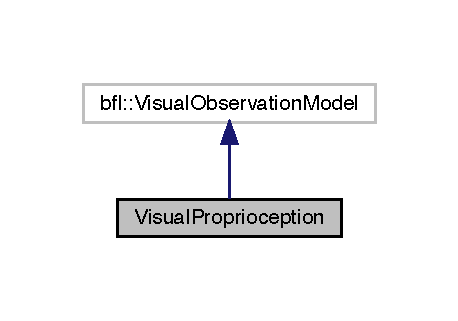
\includegraphics[width=220pt]{classVisualProprioception__inherit__graph}
\end{center}
\end{figure}
\subsection*{Public Member Functions}
\begin{DoxyCompactItemize}
\item 
\hyperlink{classVisualProprioception_a46f58af24667f43811e214023ec00dcb}{Visual\+Proprioception} (const bool use\+\_\+thumb, const bool use\+\_\+forearm, const int num\+\_\+images, const double resolution\+\_\+ratio, const yarp\+::os\+::\+Const\+String \&cam\+\_\+sel, const yarp\+::os\+::\+Const\+String \&laterality, const yarp\+::os\+::\+Const\+String \&context)
\item 
\hyperlink{classVisualProprioception_a25b2467569d795d63f806ffcdb9c2be4}{Visual\+Proprioception} (const \hyperlink{classVisualProprioception}{Visual\+Proprioception} \&proprio)
\item 
\hyperlink{classVisualProprioception_a64d833138ea6dda6e893693df8768ba9}{Visual\+Proprioception} (\hyperlink{classVisualProprioception}{Visual\+Proprioception} \&\&proprio) noexcept
\item 
\hyperlink{classVisualProprioception_a7c108406fb3ab7e381b15f8e06325513}{$\sim$\+Visual\+Proprioception} () noexcept
\item 
\hyperlink{classVisualProprioception}{Visual\+Proprioception} \& \hyperlink{classVisualProprioception_a86f418db34161e128fabf2572ef4e880}{operator=} (const \hyperlink{classVisualProprioception}{Visual\+Proprioception} \&proprio)
\item 
\hyperlink{classVisualProprioception}{Visual\+Proprioception} \& \hyperlink{classVisualProprioception_adfec67b962ad60f2afa575e681b44f3f}{operator=} (\hyperlink{classVisualProprioception}{Visual\+Proprioception} \&\&proprio) noexcept
\item 
void \hyperlink{classVisualProprioception_a9ca620e3c2dde045da52f34a600daa47}{observe} (const Eigen\+::\+Ref$<$ const Eigen\+::\+Matrix\+Xf $>$ \&cur\+\_\+states, cv\+::\+Output\+Array observations) override
\item 
bool \hyperlink{classVisualProprioception_a59835a3e089f463855de8e228fc4fd91}{set\+Property} (const std\+::string property) override
\item 
int \hyperlink{classVisualProprioception_a0b3a18baa3f51b4c88155c87ab48759a}{get\+O\+G\+L\+Tiles\+Number} ()
\item 
int \hyperlink{classVisualProprioception_ac0f57686b122f7ab867d9715281692a2}{get\+O\+G\+L\+Tiles\+Rows} ()
\item 
int \hyperlink{classVisualProprioception_a1f292b50c80393a45c557f83c82f26fd}{get\+O\+G\+L\+Tiles\+Cols} ()
\item 
unsigned int \hyperlink{classVisualProprioception_ac0507d6a1074bce7d5b6219a296977a5}{get\+Cam\+Width} ()
\item 
unsigned int \hyperlink{classVisualProprioception_a79a29f5b902dc1010c6e4def39e3e50d}{get\+Cam\+Height} ()
\item 
float \hyperlink{classVisualProprioception_a91eb7689001066cc251ebc4aa45e361e}{get\+Cam\+Fx} ()
\item 
float \hyperlink{classVisualProprioception_ad10ced05538f8f5f86b4c320e857bb19}{get\+Cam\+Fy} ()
\item 
float \hyperlink{classVisualProprioception_aca4a0fe7a02cdab6fa8587fd0341d824}{get\+Cam\+Cx} ()
\item 
float \hyperlink{classVisualProprioception_a1fb91fd83b8bf70134f36b3c8f3023b5}{get\+Cam\+Cy} ()
\end{DoxyCompactItemize}
\subsection*{Protected Member Functions}
\begin{DoxyCompactItemize}
\item 
yarp\+::sig\+::\+Matrix \hyperlink{classVisualProprioception_a30b0283a5c8b29bdf828c291e7868e51}{get\+InvertedH} (const double a, const double d, const double alpha, const double offset, const double q)
\item 
bool \hyperlink{classVisualProprioception_aaa7b46247c25b4e69a389b82472caadf}{open\+Gaze\+Controller} ()
\item 
bool \hyperlink{classVisualProprioception_aade0b47250e8315166b36f7b731d360d}{open\+Analogs} ()
\item 
bool \hyperlink{classVisualProprioception_a0d7954358702576e252efd76694d9a18}{close\+Analogs} ()
\item 
bool \hyperlink{classVisualProprioception_a23b9c75f9a3c44442a371676a0379a19}{seti\+Cub\+Params} ()
\item 
void \hyperlink{classVisualProprioception_afe0bc2a5d6fea18d75764ed12755f3ee}{set\+Arm\+Joints} (const yarp\+::sig\+::\+Vector \&q)
\item 
void \hyperlink{classVisualProprioception_ae701fa6d07822f151bfb2bce4384fb32}{set\+Arm\+Joints} (const yarp\+::sig\+::\+Vector \&q, const yarp\+::sig\+::\+Vector \&analogs, const yarp\+::sig\+::\+Matrix \&analog\+\_\+bounds)
\item 
void \hyperlink{classVisualProprioception_a06131e57aab757389277f6c06bbd6dc7}{get\+Model\+Pose} (const Eigen\+::\+Ref$<$ const Eigen\+::\+Matrix\+Xf $>$ \&cur\+\_\+states, std\+::vector$<$ Superimpose\+::\+Model\+Pose\+Container $>$ \&hand\+\_\+poses)
\item 
yarp\+::sig\+::\+Vector \hyperlink{classVisualProprioception_a9a1a2dd7b57fc600388244a3001b16ad}{read\+Arm\+Encoders} ()
\item 
yarp\+::sig\+::\+Vector \hyperlink{classVisualProprioception_a3bf5b9321ccf560bb3955cbe17fc5cab}{read\+Torso} ()
\item 
yarp\+::sig\+::\+Vector \hyperlink{classVisualProprioception_af3370849532d77174f5848f415c08e9e}{read\+Root\+To\+Fingers} ()
\item 
yarp\+::sig\+::\+Vector \hyperlink{classVisualProprioception_aa0ce08aa7f8fa882ade6997a1c9297ad}{read\+Root\+To\+Eye} (const yarp\+::os\+::\+Const\+String cam\+\_\+sel)
\item 
bool \hyperlink{classVisualProprioception_ab7be48b8a9dae0913d7554c3e30ad9e4}{file\+\_\+found} (const yarp\+::os\+::\+Const\+String \&file)
\end{DoxyCompactItemize}
\subsection*{Protected Attributes}
\begin{DoxyCompactItemize}
\item 
yarp\+::os\+::\+Const\+String \hyperlink{classVisualProprioception_ac23b912f12c8c4b639d12f343ca4fef4}{log\+\_\+\+I\+D\+\_\+} = \char`\"{}\mbox{[}Visual\+Proprioception\mbox{]}\char`\"{}
\item 
yarp\+::os\+::\+Const\+String \hyperlink{classVisualProprioception_a03d34b9887450f1def5b22b3358ea99c}{laterality\+\_\+}
\item 
yarp\+::dev\+::\+Poly\+Driver \hyperlink{classVisualProprioception_a73058b557c8169f92920f599ff0f7319}{drv\+\_\+gaze\+\_\+}
\item 
yarp\+::dev\+::\+I\+Gaze\+Control $\ast$ \hyperlink{classVisualProprioception_a775bf77a04b5c23488e53a58b47d7e20}{itf\+\_\+gaze\+\_\+}
\item 
i\+Cub\+::i\+Kin\+::i\+Cub\+Arm \hyperlink{classVisualProprioception_a4031f349da8660db553cccf2e2eed709}{icub\+\_\+arm\+\_\+}
\item 
i\+Cub\+::i\+Kin\+::i\+Cub\+Finger \hyperlink{classVisualProprioception_a629e04a45391f571094e4ae8a8dedbff}{icub\+\_\+kin\+\_\+finger\+\_\+} \mbox{[}3\mbox{]}
\item 
i\+Cub\+::i\+Kin\+::i\+Cub\+Eye \hyperlink{classVisualProprioception_ab19c8d684a0be7316a4dbb4e528ea784}{icub\+\_\+kin\+\_\+eye\+\_\+}
\item 
yarp\+::os\+::\+Buffered\+Port$<$ yarp\+::os\+::\+Bottle $>$ \hyperlink{classVisualProprioception_a1499b951384754d12a31c66fd88385b9}{port\+\_\+head\+\_\+enc\+\_\+}
\item 
yarp\+::os\+::\+Buffered\+Port$<$ yarp\+::os\+::\+Bottle $>$ \hyperlink{classVisualProprioception_acc3edbcc142167ccd748b1953fd08983}{port\+\_\+torso\+\_\+enc\+\_\+}
\item 
yarp\+::os\+::\+Buffered\+Port$<$ yarp\+::os\+::\+Bottle $>$ \hyperlink{classVisualProprioception_a9cafb14a81554af9192456cf2f29f12b}{port\+\_\+arm\+\_\+enc\+\_\+}
\item 
yarp\+::dev\+::\+Poly\+Driver \hyperlink{classVisualProprioception_af3518d76b3cac4b3fbfcb3b89ce695f1}{drv\+\_\+right\+\_\+hand\+\_\+analog\+\_\+}
\item 
yarp\+::dev\+::\+I\+Analog\+Sensor $\ast$ \hyperlink{classVisualProprioception_a16a22e76ad42cd33fbeacd47aa408a74}{itf\+\_\+right\+\_\+hand\+\_\+analog\+\_\+}
\item 
yarp\+::sig\+::\+Matrix \hyperlink{classVisualProprioception_aba826482fa47277e17277ab6b82b8039}{right\+\_\+hand\+\_\+analogs\+\_\+bounds\+\_\+}
\item 
bool \hyperlink{classVisualProprioception_a86284ecba20206e3ecb3125fc90f3ce8}{analogs\+\_\+} = false
\item 
yarp\+::os\+::\+Const\+String \hyperlink{classVisualProprioception_af0e11e8cc5facba0c725fac0b51be679}{cam\+\_\+sel\+\_\+}
\item 
double \hyperlink{classVisualProprioception_ab98ec8641e0cfbed4628e11dd10c9fb8}{cam\+\_\+x\+\_\+} \mbox{[}3\mbox{]}
\item 
double \hyperlink{classVisualProprioception_ae3278b7356ddf3fe357cc74129988521}{cam\+\_\+o\+\_\+} \mbox{[}4\mbox{]}
\item 
unsigned int \hyperlink{classVisualProprioception_aa432bf481b6dd29f2701b095f68b1e19}{cam\+\_\+width\+\_\+}
\item 
unsigned int \hyperlink{classVisualProprioception_a220e87c836c81743f3602da5cc3acebf}{cam\+\_\+height\+\_\+}
\item 
float \hyperlink{classVisualProprioception_a24c5fd2daa8ebf8837ec2746feb98bef}{cam\+\_\+fx\+\_\+}
\item 
float \hyperlink{classVisualProprioception_a8539c7bfe046289d21f82c3617da7896}{cam\+\_\+cx\+\_\+}
\item 
float \hyperlink{classVisualProprioception_a9ca32d1a6bbaf726c980871159b1e21c}{cam\+\_\+fy\+\_\+}
\item 
float \hyperlink{classVisualProprioception_ada8161ede00c312b8b2422deb5aa29e7}{cam\+\_\+cy\+\_\+}
\item 
double \hyperlink{classVisualProprioception_abf67fe6231fc4ecb742ccf9995169e62}{resolution\+\_\+ratio\+\_\+}
\item 
bool \hyperlink{classVisualProprioception_a1c25db32433ee1965a74b3b1af8a4f97}{use\+\_\+thumb\+\_\+}
\item 
bool \hyperlink{classVisualProprioception_a86e0db2eddb88029d98fdc5b4e31dc02}{use\+\_\+forearm\+\_\+}
\item 
S\+I\+C\+A\+D\+::\+Model\+Path\+Container \hyperlink{classVisualProprioception_ae7488d918a9c1893192622cd371d0277}{cad\+\_\+obj\+\_\+}
\item 
S\+I\+C\+AD $\ast$ \hyperlink{classVisualProprioception_aac9aae5f3844b662bd2918273d850120}{si\+\_\+cad\+\_\+}
\item 
int \hyperlink{classVisualProprioception_ac93a3e13b787e20720ff37dfc1e7fbb4}{ogl\+\_\+tiles\+\_\+rows\+\_\+}
\item 
int \hyperlink{classVisualProprioception_a23cd7f7cc9cbbf0e8430c858d7e7bce0}{ogl\+\_\+tiles\+\_\+cols\+\_\+}
\end{DoxyCompactItemize}


\subsection{Detailed Description}


Definition at line 20 of file Visual\+Proprioception.\+h.



\subsection{Constructor \& Destructor Documentation}
\mbox{\Hypertarget{classVisualProprioception_a46f58af24667f43811e214023ec00dcb}\label{classVisualProprioception_a46f58af24667f43811e214023ec00dcb}} 
\index{Visual\+Proprioception@{Visual\+Proprioception}!Visual\+Proprioception@{Visual\+Proprioception}}
\index{Visual\+Proprioception@{Visual\+Proprioception}!Visual\+Proprioception@{Visual\+Proprioception}}
\subsubsection{\texorpdfstring{Visual\+Proprioception()}{VisualProprioception()}\hspace{0.1cm}{\footnotesize\ttfamily [1/3]}}
{\footnotesize\ttfamily Visual\+Proprioception\+::\+Visual\+Proprioception (\begin{DoxyParamCaption}\item[{const bool}]{use\+\_\+thumb,  }\item[{const bool}]{use\+\_\+forearm,  }\item[{const int}]{num\+\_\+images,  }\item[{const double}]{resolution\+\_\+ratio,  }\item[{const yarp\+::os\+::\+Const\+String \&}]{cam\+\_\+sel,  }\item[{const yarp\+::os\+::\+Const\+String \&}]{laterality,  }\item[{const yarp\+::os\+::\+Const\+String \&}]{context }\end{DoxyParamCaption})}

\mbox{\Hypertarget{classVisualProprioception_a25b2467569d795d63f806ffcdb9c2be4}\label{classVisualProprioception_a25b2467569d795d63f806ffcdb9c2be4}} 
\index{Visual\+Proprioception@{Visual\+Proprioception}!Visual\+Proprioception@{Visual\+Proprioception}}
\index{Visual\+Proprioception@{Visual\+Proprioception}!Visual\+Proprioception@{Visual\+Proprioception}}
\subsubsection{\texorpdfstring{Visual\+Proprioception()}{VisualProprioception()}\hspace{0.1cm}{\footnotesize\ttfamily [2/3]}}
{\footnotesize\ttfamily Visual\+Proprioception\+::\+Visual\+Proprioception (\begin{DoxyParamCaption}\item[{const \hyperlink{classVisualProprioception}{Visual\+Proprioception} \&}]{proprio }\end{DoxyParamCaption})}



Definition at line 263 of file Visual\+Proprioception.\+cpp.



References cam\+\_\+o\+\_\+, cam\+\_\+x\+\_\+, icub\+\_\+arm\+\_\+, and icub\+\_\+kin\+\_\+finger\+\_\+.

\mbox{\Hypertarget{classVisualProprioception_a64d833138ea6dda6e893693df8768ba9}\label{classVisualProprioception_a64d833138ea6dda6e893693df8768ba9}} 
\index{Visual\+Proprioception@{Visual\+Proprioception}!Visual\+Proprioception@{Visual\+Proprioception}}
\index{Visual\+Proprioception@{Visual\+Proprioception}!Visual\+Proprioception@{Visual\+Proprioception}}
\subsubsection{\texorpdfstring{Visual\+Proprioception()}{VisualProprioception()}\hspace{0.1cm}{\footnotesize\ttfamily [3/3]}}
{\footnotesize\ttfamily Visual\+Proprioception\+::\+Visual\+Proprioception (\begin{DoxyParamCaption}\item[{\hyperlink{classVisualProprioception}{Visual\+Proprioception} \&\&}]{proprio }\end{DoxyParamCaption})\hspace{0.3cm}{\ttfamily [noexcept]}}



Definition at line 290 of file Visual\+Proprioception.\+cpp.



References cam\+\_\+o\+\_\+, cam\+\_\+x\+\_\+, and icub\+\_\+kin\+\_\+finger\+\_\+.

\mbox{\Hypertarget{classVisualProprioception_a7c108406fb3ab7e381b15f8e06325513}\label{classVisualProprioception_a7c108406fb3ab7e381b15f8e06325513}} 
\index{Visual\+Proprioception@{Visual\+Proprioception}!````~Visual\+Proprioception@{$\sim$\+Visual\+Proprioception}}
\index{````~Visual\+Proprioception@{$\sim$\+Visual\+Proprioception}!Visual\+Proprioception@{Visual\+Proprioception}}
\subsubsection{\texorpdfstring{$\sim$\+Visual\+Proprioception()}{~VisualProprioception()}}
{\footnotesize\ttfamily Visual\+Proprioception\+::$\sim$\+Visual\+Proprioception (\begin{DoxyParamCaption}{ }\end{DoxyParamCaption})\hspace{0.3cm}{\ttfamily [noexcept]}}



Definition at line 250 of file Visual\+Proprioception.\+cpp.



References Play\+Gate\+Pose\+::port\+\_\+arm\+\_\+enc\+\_\+, and Play\+Gate\+Pose\+::port\+\_\+torso\+\_\+enc\+\_\+.



\subsection{Member Function Documentation}
\mbox{\Hypertarget{classVisualProprioception_a0d7954358702576e252efd76694d9a18}\label{classVisualProprioception_a0d7954358702576e252efd76694d9a18}} 
\index{Visual\+Proprioception@{Visual\+Proprioception}!close\+Analogs@{close\+Analogs}}
\index{close\+Analogs@{close\+Analogs}!Visual\+Proprioception@{Visual\+Proprioception}}
\subsubsection{\texorpdfstring{close\+Analogs()}{closeAnalogs()}}
{\footnotesize\ttfamily bool Visual\+Proprioception\+::close\+Analogs (\begin{DoxyParamCaption}{ }\end{DoxyParamCaption})\hspace{0.3cm}{\ttfamily [protected]}}



Definition at line 719 of file Visual\+Proprioception.\+cpp.



References analogs\+\_\+, and drv\+\_\+right\+\_\+hand\+\_\+analog\+\_\+.



Referenced by set\+Property().

\mbox{\Hypertarget{classVisualProprioception_ab7be48b8a9dae0913d7554c3e30ad9e4}\label{classVisualProprioception_ab7be48b8a9dae0913d7554c3e30ad9e4}} 
\index{Visual\+Proprioception@{Visual\+Proprioception}!file\+\_\+found@{file\+\_\+found}}
\index{file\+\_\+found@{file\+\_\+found}!Visual\+Proprioception@{Visual\+Proprioception}}
\subsubsection{\texorpdfstring{file\+\_\+found()}{file\_found()}}
{\footnotesize\ttfamily bool Visual\+Proprioception\+::file\+\_\+found (\begin{DoxyParamCaption}\item[{const yarp\+::os\+::\+Const\+String \&}]{file }\end{DoxyParamCaption})\hspace{0.3cm}{\ttfamily [protected]}}



Definition at line 541 of file Visual\+Proprioception.\+cpp.



References log\+\_\+\+I\+D\+\_\+.

\mbox{\Hypertarget{classVisualProprioception_aca4a0fe7a02cdab6fa8587fd0341d824}\label{classVisualProprioception_aca4a0fe7a02cdab6fa8587fd0341d824}} 
\index{Visual\+Proprioception@{Visual\+Proprioception}!get\+Cam\+Cx@{get\+Cam\+Cx}}
\index{get\+Cam\+Cx@{get\+Cam\+Cx}!Visual\+Proprioception@{Visual\+Proprioception}}
\subsubsection{\texorpdfstring{get\+Cam\+Cx()}{getCamCx()}}
{\footnotesize\ttfamily float Visual\+Proprioception\+::get\+Cam\+Cx (\begin{DoxyParamCaption}{ }\end{DoxyParamCaption})}



Definition at line 595 of file Visual\+Proprioception.\+cpp.



References cam\+\_\+cx\+\_\+.

\mbox{\Hypertarget{classVisualProprioception_a1fb91fd83b8bf70134f36b3c8f3023b5}\label{classVisualProprioception_a1fb91fd83b8bf70134f36b3c8f3023b5}} 
\index{Visual\+Proprioception@{Visual\+Proprioception}!get\+Cam\+Cy@{get\+Cam\+Cy}}
\index{get\+Cam\+Cy@{get\+Cam\+Cy}!Visual\+Proprioception@{Visual\+Proprioception}}
\subsubsection{\texorpdfstring{get\+Cam\+Cy()}{getCamCy()}}
{\footnotesize\ttfamily float Visual\+Proprioception\+::get\+Cam\+Cy (\begin{DoxyParamCaption}{ }\end{DoxyParamCaption})}



Definition at line 601 of file Visual\+Proprioception.\+cpp.



References cam\+\_\+cy\+\_\+.

\mbox{\Hypertarget{classVisualProprioception_a91eb7689001066cc251ebc4aa45e361e}\label{classVisualProprioception_a91eb7689001066cc251ebc4aa45e361e}} 
\index{Visual\+Proprioception@{Visual\+Proprioception}!get\+Cam\+Fx@{get\+Cam\+Fx}}
\index{get\+Cam\+Fx@{get\+Cam\+Fx}!Visual\+Proprioception@{Visual\+Proprioception}}
\subsubsection{\texorpdfstring{get\+Cam\+Fx()}{getCamFx()}}
{\footnotesize\ttfamily float Visual\+Proprioception\+::get\+Cam\+Fx (\begin{DoxyParamCaption}{ }\end{DoxyParamCaption})}



Definition at line 583 of file Visual\+Proprioception.\+cpp.



References cam\+\_\+fx\+\_\+.

\mbox{\Hypertarget{classVisualProprioception_ad10ced05538f8f5f86b4c320e857bb19}\label{classVisualProprioception_ad10ced05538f8f5f86b4c320e857bb19}} 
\index{Visual\+Proprioception@{Visual\+Proprioception}!get\+Cam\+Fy@{get\+Cam\+Fy}}
\index{get\+Cam\+Fy@{get\+Cam\+Fy}!Visual\+Proprioception@{Visual\+Proprioception}}
\subsubsection{\texorpdfstring{get\+Cam\+Fy()}{getCamFy()}}
{\footnotesize\ttfamily float Visual\+Proprioception\+::get\+Cam\+Fy (\begin{DoxyParamCaption}{ }\end{DoxyParamCaption})}



Definition at line 589 of file Visual\+Proprioception.\+cpp.



References cam\+\_\+fy\+\_\+.

\mbox{\Hypertarget{classVisualProprioception_a79a29f5b902dc1010c6e4def39e3e50d}\label{classVisualProprioception_a79a29f5b902dc1010c6e4def39e3e50d}} 
\index{Visual\+Proprioception@{Visual\+Proprioception}!get\+Cam\+Height@{get\+Cam\+Height}}
\index{get\+Cam\+Height@{get\+Cam\+Height}!Visual\+Proprioception@{Visual\+Proprioception}}
\subsubsection{\texorpdfstring{get\+Cam\+Height()}{getCamHeight()}}
{\footnotesize\ttfamily unsigned int Visual\+Proprioception\+::get\+Cam\+Height (\begin{DoxyParamCaption}{ }\end{DoxyParamCaption})}



Definition at line 577 of file Visual\+Proprioception.\+cpp.



References cam\+\_\+height\+\_\+.

\mbox{\Hypertarget{classVisualProprioception_ac0507d6a1074bce7d5b6219a296977a5}\label{classVisualProprioception_ac0507d6a1074bce7d5b6219a296977a5}} 
\index{Visual\+Proprioception@{Visual\+Proprioception}!get\+Cam\+Width@{get\+Cam\+Width}}
\index{get\+Cam\+Width@{get\+Cam\+Width}!Visual\+Proprioception@{Visual\+Proprioception}}
\subsubsection{\texorpdfstring{get\+Cam\+Width()}{getCamWidth()}}
{\footnotesize\ttfamily unsigned int Visual\+Proprioception\+::get\+Cam\+Width (\begin{DoxyParamCaption}{ }\end{DoxyParamCaption})}



Definition at line 571 of file Visual\+Proprioception.\+cpp.



References cam\+\_\+width\+\_\+.

\mbox{\Hypertarget{classVisualProprioception_a30b0283a5c8b29bdf828c291e7868e51}\label{classVisualProprioception_a30b0283a5c8b29bdf828c291e7868e51}} 
\index{Visual\+Proprioception@{Visual\+Proprioception}!get\+InvertedH@{get\+InvertedH}}
\index{get\+InvertedH@{get\+InvertedH}!Visual\+Proprioception@{Visual\+Proprioception}}
\subsubsection{\texorpdfstring{get\+Inverted\+H()}{getInvertedH()}}
{\footnotesize\ttfamily yarp\+::sig\+::\+Matrix Visual\+Proprioception\+::get\+InvertedH (\begin{DoxyParamCaption}\item[{const double}]{a,  }\item[{const double}]{d,  }\item[{const double}]{alpha,  }\item[{const double}]{offset,  }\item[{const double}]{q }\end{DoxyParamCaption})\hspace{0.3cm}{\ttfamily [protected]}}



Definition at line 607 of file Visual\+Proprioception.\+cpp.



Referenced by get\+Model\+Pose().

\mbox{\Hypertarget{classVisualProprioception_a06131e57aab757389277f6c06bbd6dc7}\label{classVisualProprioception_a06131e57aab757389277f6c06bbd6dc7}} 
\index{Visual\+Proprioception@{Visual\+Proprioception}!get\+Model\+Pose@{get\+Model\+Pose}}
\index{get\+Model\+Pose@{get\+Model\+Pose}!Visual\+Proprioception@{Visual\+Proprioception}}
\subsubsection{\texorpdfstring{get\+Model\+Pose()}{getModelPose()}}
{\footnotesize\ttfamily void Visual\+Proprioception\+::get\+Model\+Pose (\begin{DoxyParamCaption}\item[{const Eigen\+::\+Ref$<$ const Eigen\+::\+Matrix\+Xf $>$ \&}]{cur\+\_\+states,  }\item[{std\+::vector$<$ Superimpose\+::\+Model\+Pose\+Container $>$ \&}]{hand\+\_\+poses }\end{DoxyParamCaption})\hspace{0.3cm}{\ttfamily [protected]}}



Definition at line 374 of file Visual\+Proprioception.\+cpp.



References get\+Inverted\+H(), icub\+\_\+arm\+\_\+, icub\+\_\+kin\+\_\+finger\+\_\+, use\+\_\+forearm\+\_\+, and use\+\_\+thumb\+\_\+.



Referenced by observe().

Here is the call graph for this function\+:
\nopagebreak
\begin{figure}[H]
\begin{center}
\leavevmode
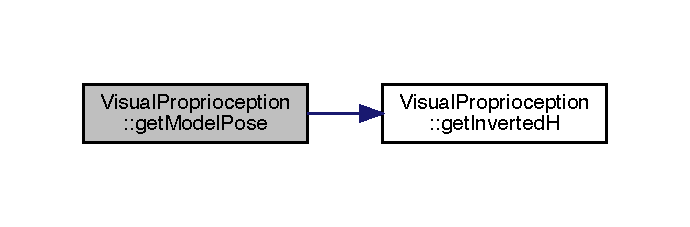
\includegraphics[width=331pt]{classVisualProprioception_a06131e57aab757389277f6c06bbd6dc7_cgraph}
\end{center}
\end{figure}
\mbox{\Hypertarget{classVisualProprioception_a1f292b50c80393a45c557f83c82f26fd}\label{classVisualProprioception_a1f292b50c80393a45c557f83c82f26fd}} 
\index{Visual\+Proprioception@{Visual\+Proprioception}!get\+O\+G\+L\+Tiles\+Cols@{get\+O\+G\+L\+Tiles\+Cols}}
\index{get\+O\+G\+L\+Tiles\+Cols@{get\+O\+G\+L\+Tiles\+Cols}!Visual\+Proprioception@{Visual\+Proprioception}}
\subsubsection{\texorpdfstring{get\+O\+G\+L\+Tiles\+Cols()}{getOGLTilesCols()}}
{\footnotesize\ttfamily int Visual\+Proprioception\+::get\+O\+G\+L\+Tiles\+Cols (\begin{DoxyParamCaption}{ }\end{DoxyParamCaption})}



Definition at line 565 of file Visual\+Proprioception.\+cpp.



References si\+\_\+cad\+\_\+.

\mbox{\Hypertarget{classVisualProprioception_a0b3a18baa3f51b4c88155c87ab48759a}\label{classVisualProprioception_a0b3a18baa3f51b4c88155c87ab48759a}} 
\index{Visual\+Proprioception@{Visual\+Proprioception}!get\+O\+G\+L\+Tiles\+Number@{get\+O\+G\+L\+Tiles\+Number}}
\index{get\+O\+G\+L\+Tiles\+Number@{get\+O\+G\+L\+Tiles\+Number}!Visual\+Proprioception@{Visual\+Proprioception}}
\subsubsection{\texorpdfstring{get\+O\+G\+L\+Tiles\+Number()}{getOGLTilesNumber()}}
{\footnotesize\ttfamily int Visual\+Proprioception\+::get\+O\+G\+L\+Tiles\+Number (\begin{DoxyParamCaption}{ }\end{DoxyParamCaption})}



Definition at line 553 of file Visual\+Proprioception.\+cpp.



References si\+\_\+cad\+\_\+.

\mbox{\Hypertarget{classVisualProprioception_ac0f57686b122f7ab867d9715281692a2}\label{classVisualProprioception_ac0f57686b122f7ab867d9715281692a2}} 
\index{Visual\+Proprioception@{Visual\+Proprioception}!get\+O\+G\+L\+Tiles\+Rows@{get\+O\+G\+L\+Tiles\+Rows}}
\index{get\+O\+G\+L\+Tiles\+Rows@{get\+O\+G\+L\+Tiles\+Rows}!Visual\+Proprioception@{Visual\+Proprioception}}
\subsubsection{\texorpdfstring{get\+O\+G\+L\+Tiles\+Rows()}{getOGLTilesRows()}}
{\footnotesize\ttfamily int Visual\+Proprioception\+::get\+O\+G\+L\+Tiles\+Rows (\begin{DoxyParamCaption}{ }\end{DoxyParamCaption})}



Definition at line 559 of file Visual\+Proprioception.\+cpp.



References si\+\_\+cad\+\_\+.

\mbox{\Hypertarget{classVisualProprioception_a9ca620e3c2dde045da52f34a600daa47}\label{classVisualProprioception_a9ca620e3c2dde045da52f34a600daa47}} 
\index{Visual\+Proprioception@{Visual\+Proprioception}!observe@{observe}}
\index{observe@{observe}!Visual\+Proprioception@{Visual\+Proprioception}}
\subsubsection{\texorpdfstring{observe()}{observe()}}
{\footnotesize\ttfamily void Visual\+Proprioception\+::observe (\begin{DoxyParamCaption}\item[{const Eigen\+::\+Ref$<$ const Eigen\+::\+Matrix\+Xf $>$ \&}]{cur\+\_\+states,  }\item[{cv\+::\+Output\+Array}]{observations }\end{DoxyParamCaption})\hspace{0.3cm}{\ttfamily [override]}}



Definition at line 451 of file Visual\+Proprioception.\+cpp.



References cam\+\_\+o\+\_\+, cam\+\_\+x\+\_\+, get\+Model\+Pose(), and si\+\_\+cad\+\_\+.

Here is the call graph for this function\+:
\nopagebreak
\begin{figure}[H]
\begin{center}
\leavevmode
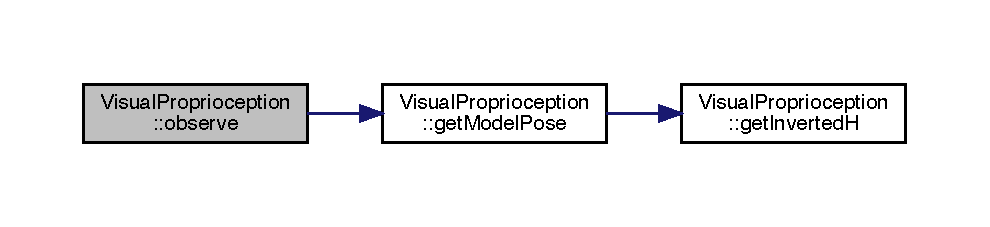
\includegraphics[width=350pt]{classVisualProprioception_a9ca620e3c2dde045da52f34a600daa47_cgraph}
\end{center}
\end{figure}
\mbox{\Hypertarget{classVisualProprioception_aade0b47250e8315166b36f7b731d360d}\label{classVisualProprioception_aade0b47250e8315166b36f7b731d360d}} 
\index{Visual\+Proprioception@{Visual\+Proprioception}!open\+Analogs@{open\+Analogs}}
\index{open\+Analogs@{open\+Analogs}!Visual\+Proprioception@{Visual\+Proprioception}}
\subsubsection{\texorpdfstring{open\+Analogs()}{openAnalogs()}}
{\footnotesize\ttfamily bool Visual\+Proprioception\+::open\+Analogs (\begin{DoxyParamCaption}{ }\end{DoxyParamCaption})\hspace{0.3cm}{\ttfamily [protected]}}



Definition at line 684 of file Visual\+Proprioception.\+cpp.



References analogs\+\_\+, cam\+\_\+sel\+\_\+, drv\+\_\+right\+\_\+hand\+\_\+analog\+\_\+, itf\+\_\+right\+\_\+hand\+\_\+analog\+\_\+, laterality\+\_\+, and log\+\_\+\+I\+D\+\_\+.



Referenced by set\+Property().

\mbox{\Hypertarget{classVisualProprioception_aaa7b46247c25b4e69a389b82472caadf}\label{classVisualProprioception_aaa7b46247c25b4e69a389b82472caadf}} 
\index{Visual\+Proprioception@{Visual\+Proprioception}!open\+Gaze\+Controller@{open\+Gaze\+Controller}}
\index{open\+Gaze\+Controller@{open\+Gaze\+Controller}!Visual\+Proprioception@{Visual\+Proprioception}}
\subsubsection{\texorpdfstring{open\+Gaze\+Controller()}{openGazeController()}}
{\footnotesize\ttfamily bool Visual\+Proprioception\+::open\+Gaze\+Controller (\begin{DoxyParamCaption}{ }\end{DoxyParamCaption})\hspace{0.3cm}{\ttfamily [protected]}}



Definition at line 655 of file Visual\+Proprioception.\+cpp.



References cam\+\_\+sel\+\_\+, drv\+\_\+gaze\+\_\+, itf\+\_\+gaze\+\_\+, and log\+\_\+\+I\+D\+\_\+.

\mbox{\Hypertarget{classVisualProprioception_a86f418db34161e128fabf2572ef4e880}\label{classVisualProprioception_a86f418db34161e128fabf2572ef4e880}} 
\index{Visual\+Proprioception@{Visual\+Proprioception}!operator=@{operator=}}
\index{operator=@{operator=}!Visual\+Proprioception@{Visual\+Proprioception}}
\subsubsection{\texorpdfstring{operator=()}{operator=()}\hspace{0.1cm}{\footnotesize\ttfamily [1/2]}}
{\footnotesize\ttfamily \hyperlink{classVisualProprioception}{Visual\+Proprioception} \& Visual\+Proprioception\+::operator= (\begin{DoxyParamCaption}\item[{const \hyperlink{classVisualProprioception}{Visual\+Proprioception} \&}]{proprio }\end{DoxyParamCaption})}



Definition at line 325 of file Visual\+Proprioception.\+cpp.

\mbox{\Hypertarget{classVisualProprioception_adfec67b962ad60f2afa575e681b44f3f}\label{classVisualProprioception_adfec67b962ad60f2afa575e681b44f3f}} 
\index{Visual\+Proprioception@{Visual\+Proprioception}!operator=@{operator=}}
\index{operator=@{operator=}!Visual\+Proprioception@{Visual\+Proprioception}}
\subsubsection{\texorpdfstring{operator=()}{operator=()}\hspace{0.1cm}{\footnotesize\ttfamily [2/2]}}
{\footnotesize\ttfamily \hyperlink{classVisualProprioception}{Visual\+Proprioception} \& Visual\+Proprioception\+::operator= (\begin{DoxyParamCaption}\item[{\hyperlink{classVisualProprioception}{Visual\+Proprioception} \&\&}]{proprio }\end{DoxyParamCaption})\hspace{0.3cm}{\ttfamily [noexcept]}}



Definition at line 334 of file Visual\+Proprioception.\+cpp.



References cad\+\_\+obj\+\_\+, cam\+\_\+o\+\_\+, cam\+\_\+x\+\_\+, icub\+\_\+arm\+\_\+, icub\+\_\+kin\+\_\+finger\+\_\+, and si\+\_\+cad\+\_\+.

\mbox{\Hypertarget{classVisualProprioception_a9a1a2dd7b57fc600388244a3001b16ad}\label{classVisualProprioception_a9a1a2dd7b57fc600388244a3001b16ad}} 
\index{Visual\+Proprioception@{Visual\+Proprioception}!read\+Arm\+Encoders@{read\+Arm\+Encoders}}
\index{read\+Arm\+Encoders@{read\+Arm\+Encoders}!Visual\+Proprioception@{Visual\+Proprioception}}
\subsubsection{\texorpdfstring{read\+Arm\+Encoders()}{readArmEncoders()}}
{\footnotesize\ttfamily yarp\+::sig\+::\+Vector Visual\+Proprioception\+::read\+Arm\+Encoders (\begin{DoxyParamCaption}{ }\end{DoxyParamCaption})\hspace{0.3cm}{\ttfamily [protected]}}

\mbox{\Hypertarget{classVisualProprioception_aa0ce08aa7f8fa882ade6997a1c9297ad}\label{classVisualProprioception_aa0ce08aa7f8fa882ade6997a1c9297ad}} 
\index{Visual\+Proprioception@{Visual\+Proprioception}!read\+Root\+To\+Eye@{read\+Root\+To\+Eye}}
\index{read\+Root\+To\+Eye@{read\+Root\+To\+Eye}!Visual\+Proprioception@{Visual\+Proprioception}}
\subsubsection{\texorpdfstring{read\+Root\+To\+Eye()}{readRootToEye()}}
{\footnotesize\ttfamily Vector Visual\+Proprioception\+::read\+Root\+To\+Eye (\begin{DoxyParamCaption}\item[{const yarp\+::os\+::\+Const\+String}]{cam\+\_\+sel }\end{DoxyParamCaption})\hspace{0.3cm}{\ttfamily [protected]}}



Definition at line 761 of file Visual\+Proprioception.\+cpp.



References port\+\_\+head\+\_\+enc\+\_\+, and read\+Torso().



Referenced by seti\+Cub\+Params().

Here is the call graph for this function\+:
\nopagebreak
\begin{figure}[H]
\begin{center}
\leavevmode
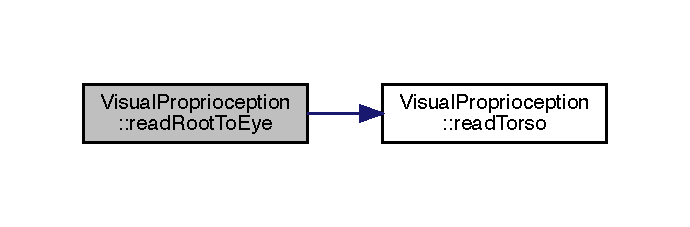
\includegraphics[width=331pt]{classVisualProprioception_aa0ce08aa7f8fa882ade6997a1c9297ad_cgraph}
\end{center}
\end{figure}
\mbox{\Hypertarget{classVisualProprioception_af3370849532d77174f5848f415c08e9e}\label{classVisualProprioception_af3370849532d77174f5848f415c08e9e}} 
\index{Visual\+Proprioception@{Visual\+Proprioception}!read\+Root\+To\+Fingers@{read\+Root\+To\+Fingers}}
\index{read\+Root\+To\+Fingers@{read\+Root\+To\+Fingers}!Visual\+Proprioception@{Visual\+Proprioception}}
\subsubsection{\texorpdfstring{read\+Root\+To\+Fingers()}{readRootToFingers()}}
{\footnotesize\ttfamily Vector Visual\+Proprioception\+::read\+Root\+To\+Fingers (\begin{DoxyParamCaption}{ }\end{DoxyParamCaption})\hspace{0.3cm}{\ttfamily [protected]}}



Definition at line 747 of file Visual\+Proprioception.\+cpp.



References port\+\_\+arm\+\_\+enc\+\_\+, and read\+Torso().



Referenced by seti\+Cub\+Params().

Here is the call graph for this function\+:
\nopagebreak
\begin{figure}[H]
\begin{center}
\leavevmode
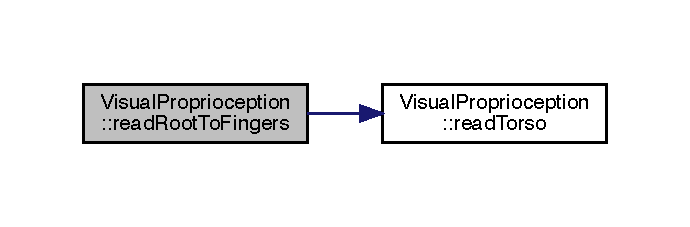
\includegraphics[width=331pt]{classVisualProprioception_af3370849532d77174f5848f415c08e9e_cgraph}
\end{center}
\end{figure}
\mbox{\Hypertarget{classVisualProprioception_a3bf5b9321ccf560bb3955cbe17fc5cab}\label{classVisualProprioception_a3bf5b9321ccf560bb3955cbe17fc5cab}} 
\index{Visual\+Proprioception@{Visual\+Proprioception}!read\+Torso@{read\+Torso}}
\index{read\+Torso@{read\+Torso}!Visual\+Proprioception@{Visual\+Proprioception}}
\subsubsection{\texorpdfstring{read\+Torso()}{readTorso()}}
{\footnotesize\ttfamily Vector Visual\+Proprioception\+::read\+Torso (\begin{DoxyParamCaption}{ }\end{DoxyParamCaption})\hspace{0.3cm}{\ttfamily [protected]}}



Definition at line 733 of file Visual\+Proprioception.\+cpp.



References port\+\_\+torso\+\_\+enc\+\_\+.



Referenced by read\+Root\+To\+Eye(), and read\+Root\+To\+Fingers().

\mbox{\Hypertarget{classVisualProprioception_afe0bc2a5d6fea18d75764ed12755f3ee}\label{classVisualProprioception_afe0bc2a5d6fea18d75764ed12755f3ee}} 
\index{Visual\+Proprioception@{Visual\+Proprioception}!set\+Arm\+Joints@{set\+Arm\+Joints}}
\index{set\+Arm\+Joints@{set\+Arm\+Joints}!Visual\+Proprioception@{Visual\+Proprioception}}
\subsubsection{\texorpdfstring{set\+Arm\+Joints()}{setArmJoints()}\hspace{0.1cm}{\footnotesize\ttfamily [1/2]}}
{\footnotesize\ttfamily void Visual\+Proprioception\+::set\+Arm\+Joints (\begin{DoxyParamCaption}\item[{const yarp\+::sig\+::\+Vector \&}]{q }\end{DoxyParamCaption})\hspace{0.3cm}{\ttfamily [protected]}}



Referenced by seti\+Cub\+Params().

\mbox{\Hypertarget{classVisualProprioception_ae701fa6d07822f151bfb2bce4384fb32}\label{classVisualProprioception_ae701fa6d07822f151bfb2bce4384fb32}} 
\index{Visual\+Proprioception@{Visual\+Proprioception}!set\+Arm\+Joints@{set\+Arm\+Joints}}
\index{set\+Arm\+Joints@{set\+Arm\+Joints}!Visual\+Proprioception@{Visual\+Proprioception}}
\subsubsection{\texorpdfstring{set\+Arm\+Joints()}{setArmJoints()}\hspace{0.1cm}{\footnotesize\ttfamily [2/2]}}
{\footnotesize\ttfamily void Visual\+Proprioception\+::set\+Arm\+Joints (\begin{DoxyParamCaption}\item[{const yarp\+::sig\+::\+Vector \&}]{q,  }\item[{const yarp\+::sig\+::\+Vector \&}]{analogs,  }\item[{const yarp\+::sig\+::\+Matrix \&}]{analog\+\_\+bounds }\end{DoxyParamCaption})\hspace{0.3cm}{\ttfamily [protected]}}

\mbox{\Hypertarget{classVisualProprioception_a23b9c75f9a3c44442a371676a0379a19}\label{classVisualProprioception_a23b9c75f9a3c44442a371676a0379a19}} 
\index{Visual\+Proprioception@{Visual\+Proprioception}!seti\+Cub\+Params@{seti\+Cub\+Params}}
\index{seti\+Cub\+Params@{seti\+Cub\+Params}!Visual\+Proprioception@{Visual\+Proprioception}}
\subsubsection{\texorpdfstring{seti\+Cub\+Params()}{setiCubParams()}}
{\footnotesize\ttfamily bool Visual\+Proprioception\+::seti\+Cub\+Params (\begin{DoxyParamCaption}{ }\end{DoxyParamCaption})\hspace{0.3cm}{\ttfamily [protected]}}



Definition at line 477 of file Visual\+Proprioception.\+cpp.



References analogs\+\_\+, cam\+\_\+o\+\_\+, cam\+\_\+sel\+\_\+, cam\+\_\+x\+\_\+, icub\+\_\+arm\+\_\+, icub\+\_\+kin\+\_\+eye\+\_\+, icub\+\_\+kin\+\_\+finger\+\_\+, itf\+\_\+right\+\_\+hand\+\_\+analog\+\_\+, read\+Root\+To\+Eye(), read\+Root\+To\+Fingers(), right\+\_\+hand\+\_\+analogs\+\_\+bounds\+\_\+, and set\+Arm\+Joints().



Referenced by set\+Property().

Here is the call graph for this function\+:
\nopagebreak
\begin{figure}[H]
\begin{center}
\leavevmode
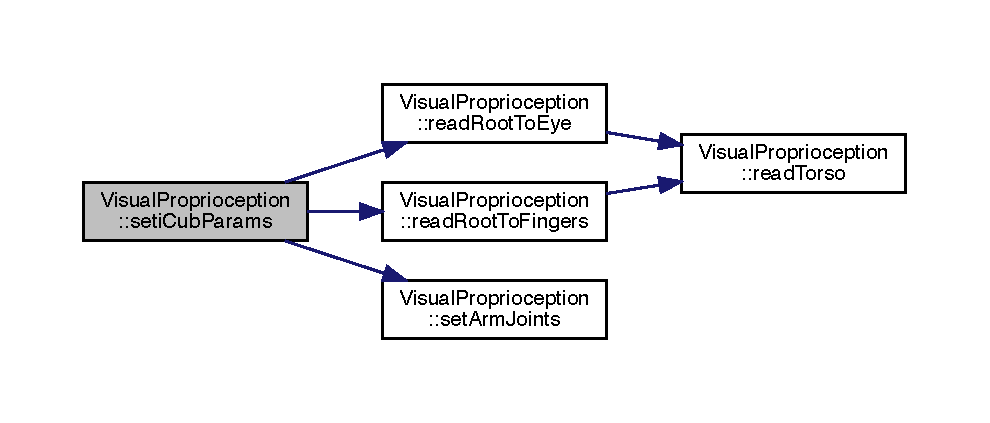
\includegraphics[width=350pt]{classVisualProprioception_a23b9c75f9a3c44442a371676a0379a19_cgraph}
\end{center}
\end{figure}
\mbox{\Hypertarget{classVisualProprioception_a59835a3e089f463855de8e228fc4fd91}\label{classVisualProprioception_a59835a3e089f463855de8e228fc4fd91}} 
\index{Visual\+Proprioception@{Visual\+Proprioception}!set\+Property@{set\+Property}}
\index{set\+Property@{set\+Property}!Visual\+Proprioception@{Visual\+Proprioception}}
\subsubsection{\texorpdfstring{set\+Property()}{setProperty()}}
{\footnotesize\ttfamily bool Visual\+Proprioception\+::set\+Property (\begin{DoxyParamCaption}\item[{const std\+::string}]{property }\end{DoxyParamCaption})\hspace{0.3cm}{\ttfamily [override]}}



Definition at line 463 of file Visual\+Proprioception.\+cpp.



References close\+Analogs(), open\+Analogs(), and seti\+Cub\+Params().

Here is the call graph for this function\+:
\nopagebreak
\begin{figure}[H]
\begin{center}
\leavevmode
\includegraphics[width=350pt]{classVisualProprioception_a59835a3e089f463855de8e228fc4fd91_cgraph}
\end{center}
\end{figure}


\subsection{Member Data Documentation}
\mbox{\Hypertarget{classVisualProprioception_a86284ecba20206e3ecb3125fc90f3ce8}\label{classVisualProprioception_a86284ecba20206e3ecb3125fc90f3ce8}} 
\index{Visual\+Proprioception@{Visual\+Proprioception}!analogs\+\_\+@{analogs\+\_\+}}
\index{analogs\+\_\+@{analogs\+\_\+}!Visual\+Proprioception@{Visual\+Proprioception}}
\subsubsection{\texorpdfstring{analogs\+\_\+}{analogs\_}}
{\footnotesize\ttfamily bool Visual\+Proprioception\+::analogs\+\_\+ = false\hspace{0.3cm}{\ttfamily [protected]}}



Definition at line 80 of file Visual\+Proprioception.\+h.



Referenced by close\+Analogs(), open\+Analogs(), and seti\+Cub\+Params().

\mbox{\Hypertarget{classVisualProprioception_ae7488d918a9c1893192622cd371d0277}\label{classVisualProprioception_ae7488d918a9c1893192622cd371d0277}} 
\index{Visual\+Proprioception@{Visual\+Proprioception}!cad\+\_\+obj\+\_\+@{cad\+\_\+obj\+\_\+}}
\index{cad\+\_\+obj\+\_\+@{cad\+\_\+obj\+\_\+}!Visual\+Proprioception@{Visual\+Proprioception}}
\subsubsection{\texorpdfstring{cad\+\_\+obj\+\_\+}{cad\_obj\_}}
{\footnotesize\ttfamily S\+I\+C\+A\+D\+::\+Model\+Path\+Container Visual\+Proprioception\+::cad\+\_\+obj\+\_\+\hspace{0.3cm}{\ttfamily [protected]}}



Definition at line 109 of file Visual\+Proprioception.\+h.



Referenced by operator=().

\mbox{\Hypertarget{classVisualProprioception_a8539c7bfe046289d21f82c3617da7896}\label{classVisualProprioception_a8539c7bfe046289d21f82c3617da7896}} 
\index{Visual\+Proprioception@{Visual\+Proprioception}!cam\+\_\+cx\+\_\+@{cam\+\_\+cx\+\_\+}}
\index{cam\+\_\+cx\+\_\+@{cam\+\_\+cx\+\_\+}!Visual\+Proprioception@{Visual\+Proprioception}}
\subsubsection{\texorpdfstring{cam\+\_\+cx\+\_\+}{cam\_cx\_}}
{\footnotesize\ttfamily float Visual\+Proprioception\+::cam\+\_\+cx\+\_\+\hspace{0.3cm}{\ttfamily [protected]}}



Definition at line 102 of file Visual\+Proprioception.\+h.



Referenced by get\+Cam\+Cx().

\mbox{\Hypertarget{classVisualProprioception_ada8161ede00c312b8b2422deb5aa29e7}\label{classVisualProprioception_ada8161ede00c312b8b2422deb5aa29e7}} 
\index{Visual\+Proprioception@{Visual\+Proprioception}!cam\+\_\+cy\+\_\+@{cam\+\_\+cy\+\_\+}}
\index{cam\+\_\+cy\+\_\+@{cam\+\_\+cy\+\_\+}!Visual\+Proprioception@{Visual\+Proprioception}}
\subsubsection{\texorpdfstring{cam\+\_\+cy\+\_\+}{cam\_cy\_}}
{\footnotesize\ttfamily float Visual\+Proprioception\+::cam\+\_\+cy\+\_\+\hspace{0.3cm}{\ttfamily [protected]}}



Definition at line 104 of file Visual\+Proprioception.\+h.



Referenced by get\+Cam\+Cy().

\mbox{\Hypertarget{classVisualProprioception_a24c5fd2daa8ebf8837ec2746feb98bef}\label{classVisualProprioception_a24c5fd2daa8ebf8837ec2746feb98bef}} 
\index{Visual\+Proprioception@{Visual\+Proprioception}!cam\+\_\+fx\+\_\+@{cam\+\_\+fx\+\_\+}}
\index{cam\+\_\+fx\+\_\+@{cam\+\_\+fx\+\_\+}!Visual\+Proprioception@{Visual\+Proprioception}}
\subsubsection{\texorpdfstring{cam\+\_\+fx\+\_\+}{cam\_fx\_}}
{\footnotesize\ttfamily float Visual\+Proprioception\+::cam\+\_\+fx\+\_\+\hspace{0.3cm}{\ttfamily [protected]}}



Definition at line 101 of file Visual\+Proprioception.\+h.



Referenced by get\+Cam\+Fx().

\mbox{\Hypertarget{classVisualProprioception_a9ca32d1a6bbaf726c980871159b1e21c}\label{classVisualProprioception_a9ca32d1a6bbaf726c980871159b1e21c}} 
\index{Visual\+Proprioception@{Visual\+Proprioception}!cam\+\_\+fy\+\_\+@{cam\+\_\+fy\+\_\+}}
\index{cam\+\_\+fy\+\_\+@{cam\+\_\+fy\+\_\+}!Visual\+Proprioception@{Visual\+Proprioception}}
\subsubsection{\texorpdfstring{cam\+\_\+fy\+\_\+}{cam\_fy\_}}
{\footnotesize\ttfamily float Visual\+Proprioception\+::cam\+\_\+fy\+\_\+\hspace{0.3cm}{\ttfamily [protected]}}



Definition at line 103 of file Visual\+Proprioception.\+h.



Referenced by get\+Cam\+Fy().

\mbox{\Hypertarget{classVisualProprioception_a220e87c836c81743f3602da5cc3acebf}\label{classVisualProprioception_a220e87c836c81743f3602da5cc3acebf}} 
\index{Visual\+Proprioception@{Visual\+Proprioception}!cam\+\_\+height\+\_\+@{cam\+\_\+height\+\_\+}}
\index{cam\+\_\+height\+\_\+@{cam\+\_\+height\+\_\+}!Visual\+Proprioception@{Visual\+Proprioception}}
\subsubsection{\texorpdfstring{cam\+\_\+height\+\_\+}{cam\_height\_}}
{\footnotesize\ttfamily unsigned int Visual\+Proprioception\+::cam\+\_\+height\+\_\+\hspace{0.3cm}{\ttfamily [protected]}}



Definition at line 100 of file Visual\+Proprioception.\+h.



Referenced by get\+Cam\+Height().

\mbox{\Hypertarget{classVisualProprioception_ae3278b7356ddf3fe357cc74129988521}\label{classVisualProprioception_ae3278b7356ddf3fe357cc74129988521}} 
\index{Visual\+Proprioception@{Visual\+Proprioception}!cam\+\_\+o\+\_\+@{cam\+\_\+o\+\_\+}}
\index{cam\+\_\+o\+\_\+@{cam\+\_\+o\+\_\+}!Visual\+Proprioception@{Visual\+Proprioception}}
\subsubsection{\texorpdfstring{cam\+\_\+o\+\_\+}{cam\_o\_}}
{\footnotesize\ttfamily double Visual\+Proprioception\+::cam\+\_\+o\+\_\+\mbox{[}4\mbox{]}\hspace{0.3cm}{\ttfamily [protected]}}



Definition at line 98 of file Visual\+Proprioception.\+h.



Referenced by observe(), operator=(), seti\+Cub\+Params(), and Visual\+Proprioception().

\mbox{\Hypertarget{classVisualProprioception_af0e11e8cc5facba0c725fac0b51be679}\label{classVisualProprioception_af0e11e8cc5facba0c725fac0b51be679}} 
\index{Visual\+Proprioception@{Visual\+Proprioception}!cam\+\_\+sel\+\_\+@{cam\+\_\+sel\+\_\+}}
\index{cam\+\_\+sel\+\_\+@{cam\+\_\+sel\+\_\+}!Visual\+Proprioception@{Visual\+Proprioception}}
\subsubsection{\texorpdfstring{cam\+\_\+sel\+\_\+}{cam\_sel\_}}
{\footnotesize\ttfamily yarp\+::os\+::\+Const\+String Visual\+Proprioception\+::cam\+\_\+sel\+\_\+\hspace{0.3cm}{\ttfamily [protected]}}



Definition at line 96 of file Visual\+Proprioception.\+h.



Referenced by open\+Analogs(), open\+Gaze\+Controller(), and seti\+Cub\+Params().

\mbox{\Hypertarget{classVisualProprioception_aa432bf481b6dd29f2701b095f68b1e19}\label{classVisualProprioception_aa432bf481b6dd29f2701b095f68b1e19}} 
\index{Visual\+Proprioception@{Visual\+Proprioception}!cam\+\_\+width\+\_\+@{cam\+\_\+width\+\_\+}}
\index{cam\+\_\+width\+\_\+@{cam\+\_\+width\+\_\+}!Visual\+Proprioception@{Visual\+Proprioception}}
\subsubsection{\texorpdfstring{cam\+\_\+width\+\_\+}{cam\_width\_}}
{\footnotesize\ttfamily unsigned int Visual\+Proprioception\+::cam\+\_\+width\+\_\+\hspace{0.3cm}{\ttfamily [protected]}}



Definition at line 99 of file Visual\+Proprioception.\+h.



Referenced by get\+Cam\+Width().

\mbox{\Hypertarget{classVisualProprioception_ab98ec8641e0cfbed4628e11dd10c9fb8}\label{classVisualProprioception_ab98ec8641e0cfbed4628e11dd10c9fb8}} 
\index{Visual\+Proprioception@{Visual\+Proprioception}!cam\+\_\+x\+\_\+@{cam\+\_\+x\+\_\+}}
\index{cam\+\_\+x\+\_\+@{cam\+\_\+x\+\_\+}!Visual\+Proprioception@{Visual\+Proprioception}}
\subsubsection{\texorpdfstring{cam\+\_\+x\+\_\+}{cam\_x\_}}
{\footnotesize\ttfamily double Visual\+Proprioception\+::cam\+\_\+x\+\_\+\mbox{[}3\mbox{]}\hspace{0.3cm}{\ttfamily [protected]}}



Definition at line 97 of file Visual\+Proprioception.\+h.



Referenced by observe(), operator=(), seti\+Cub\+Params(), and Visual\+Proprioception().

\mbox{\Hypertarget{classVisualProprioception_a73058b557c8169f92920f599ff0f7319}\label{classVisualProprioception_a73058b557c8169f92920f599ff0f7319}} 
\index{Visual\+Proprioception@{Visual\+Proprioception}!drv\+\_\+gaze\+\_\+@{drv\+\_\+gaze\+\_\+}}
\index{drv\+\_\+gaze\+\_\+@{drv\+\_\+gaze\+\_\+}!Visual\+Proprioception@{Visual\+Proprioception}}
\subsubsection{\texorpdfstring{drv\+\_\+gaze\+\_\+}{drv\_gaze\_}}
{\footnotesize\ttfamily yarp\+::dev\+::\+Poly\+Driver Visual\+Proprioception\+::drv\+\_\+gaze\+\_\+\hspace{0.3cm}{\ttfamily [protected]}}



Definition at line 62 of file Visual\+Proprioception.\+h.



Referenced by open\+Gaze\+Controller().

\mbox{\Hypertarget{classVisualProprioception_af3518d76b3cac4b3fbfcb3b89ce695f1}\label{classVisualProprioception_af3518d76b3cac4b3fbfcb3b89ce695f1}} 
\index{Visual\+Proprioception@{Visual\+Proprioception}!drv\+\_\+right\+\_\+hand\+\_\+analog\+\_\+@{drv\+\_\+right\+\_\+hand\+\_\+analog\+\_\+}}
\index{drv\+\_\+right\+\_\+hand\+\_\+analog\+\_\+@{drv\+\_\+right\+\_\+hand\+\_\+analog\+\_\+}!Visual\+Proprioception@{Visual\+Proprioception}}
\subsubsection{\texorpdfstring{drv\+\_\+right\+\_\+hand\+\_\+analog\+\_\+}{drv\_right\_hand\_analog\_}}
{\footnotesize\ttfamily yarp\+::dev\+::\+Poly\+Driver Visual\+Proprioception\+::drv\+\_\+right\+\_\+hand\+\_\+analog\+\_\+\hspace{0.3cm}{\ttfamily [protected]}}



Definition at line 70 of file Visual\+Proprioception.\+h.



Referenced by close\+Analogs(), and open\+Analogs().

\mbox{\Hypertarget{classVisualProprioception_a4031f349da8660db553cccf2e2eed709}\label{classVisualProprioception_a4031f349da8660db553cccf2e2eed709}} 
\index{Visual\+Proprioception@{Visual\+Proprioception}!icub\+\_\+arm\+\_\+@{icub\+\_\+arm\+\_\+}}
\index{icub\+\_\+arm\+\_\+@{icub\+\_\+arm\+\_\+}!Visual\+Proprioception@{Visual\+Proprioception}}
\subsubsection{\texorpdfstring{icub\+\_\+arm\+\_\+}{icub\_arm\_}}
{\footnotesize\ttfamily i\+Cub\+::i\+Kin\+::i\+Cub\+Arm Visual\+Proprioception\+::icub\+\_\+arm\+\_\+\hspace{0.3cm}{\ttfamily [protected]}}



Definition at line 64 of file Visual\+Proprioception.\+h.



Referenced by get\+Model\+Pose(), operator=(), seti\+Cub\+Params(), and Visual\+Proprioception().

\mbox{\Hypertarget{classVisualProprioception_ab19c8d684a0be7316a4dbb4e528ea784}\label{classVisualProprioception_ab19c8d684a0be7316a4dbb4e528ea784}} 
\index{Visual\+Proprioception@{Visual\+Proprioception}!icub\+\_\+kin\+\_\+eye\+\_\+@{icub\+\_\+kin\+\_\+eye\+\_\+}}
\index{icub\+\_\+kin\+\_\+eye\+\_\+@{icub\+\_\+kin\+\_\+eye\+\_\+}!Visual\+Proprioception@{Visual\+Proprioception}}
\subsubsection{\texorpdfstring{icub\+\_\+kin\+\_\+eye\+\_\+}{icub\_kin\_eye\_}}
{\footnotesize\ttfamily i\+Cub\+::i\+Kin\+::i\+Cub\+Eye Visual\+Proprioception\+::icub\+\_\+kin\+\_\+eye\+\_\+\hspace{0.3cm}{\ttfamily [protected]}}



Definition at line 66 of file Visual\+Proprioception.\+h.



Referenced by seti\+Cub\+Params().

\mbox{\Hypertarget{classVisualProprioception_a629e04a45391f571094e4ae8a8dedbff}\label{classVisualProprioception_a629e04a45391f571094e4ae8a8dedbff}} 
\index{Visual\+Proprioception@{Visual\+Proprioception}!icub\+\_\+kin\+\_\+finger\+\_\+@{icub\+\_\+kin\+\_\+finger\+\_\+}}
\index{icub\+\_\+kin\+\_\+finger\+\_\+@{icub\+\_\+kin\+\_\+finger\+\_\+}!Visual\+Proprioception@{Visual\+Proprioception}}
\subsubsection{\texorpdfstring{icub\+\_\+kin\+\_\+finger\+\_\+}{icub\_kin\_finger\_}}
{\footnotesize\ttfamily i\+Cub\+::i\+Kin\+::i\+Cub\+Finger Visual\+Proprioception\+::icub\+\_\+kin\+\_\+finger\+\_\+\mbox{[}3\mbox{]}\hspace{0.3cm}{\ttfamily [protected]}}



Definition at line 65 of file Visual\+Proprioception.\+h.



Referenced by get\+Model\+Pose(), operator=(), seti\+Cub\+Params(), and Visual\+Proprioception().

\mbox{\Hypertarget{classVisualProprioception_a775bf77a04b5c23488e53a58b47d7e20}\label{classVisualProprioception_a775bf77a04b5c23488e53a58b47d7e20}} 
\index{Visual\+Proprioception@{Visual\+Proprioception}!itf\+\_\+gaze\+\_\+@{itf\+\_\+gaze\+\_\+}}
\index{itf\+\_\+gaze\+\_\+@{itf\+\_\+gaze\+\_\+}!Visual\+Proprioception@{Visual\+Proprioception}}
\subsubsection{\texorpdfstring{itf\+\_\+gaze\+\_\+}{itf\_gaze\_}}
{\footnotesize\ttfamily yarp\+::dev\+::\+I\+Gaze\+Control$\ast$ Visual\+Proprioception\+::itf\+\_\+gaze\+\_\+\hspace{0.3cm}{\ttfamily [protected]}}



Definition at line 63 of file Visual\+Proprioception.\+h.



Referenced by open\+Gaze\+Controller().

\mbox{\Hypertarget{classVisualProprioception_a16a22e76ad42cd33fbeacd47aa408a74}\label{classVisualProprioception_a16a22e76ad42cd33fbeacd47aa408a74}} 
\index{Visual\+Proprioception@{Visual\+Proprioception}!itf\+\_\+right\+\_\+hand\+\_\+analog\+\_\+@{itf\+\_\+right\+\_\+hand\+\_\+analog\+\_\+}}
\index{itf\+\_\+right\+\_\+hand\+\_\+analog\+\_\+@{itf\+\_\+right\+\_\+hand\+\_\+analog\+\_\+}!Visual\+Proprioception@{Visual\+Proprioception}}
\subsubsection{\texorpdfstring{itf\+\_\+right\+\_\+hand\+\_\+analog\+\_\+}{itf\_right\_hand\_analog\_}}
{\footnotesize\ttfamily yarp\+::dev\+::\+I\+Analog\+Sensor$\ast$ Visual\+Proprioception\+::itf\+\_\+right\+\_\+hand\+\_\+analog\+\_\+\hspace{0.3cm}{\ttfamily [protected]}}



Definition at line 71 of file Visual\+Proprioception.\+h.



Referenced by open\+Analogs(), and seti\+Cub\+Params().

\mbox{\Hypertarget{classVisualProprioception_a03d34b9887450f1def5b22b3358ea99c}\label{classVisualProprioception_a03d34b9887450f1def5b22b3358ea99c}} 
\index{Visual\+Proprioception@{Visual\+Proprioception}!laterality\+\_\+@{laterality\+\_\+}}
\index{laterality\+\_\+@{laterality\+\_\+}!Visual\+Proprioception@{Visual\+Proprioception}}
\subsubsection{\texorpdfstring{laterality\+\_\+}{laterality\_}}
{\footnotesize\ttfamily yarp\+::os\+::\+Const\+String Visual\+Proprioception\+::laterality\+\_\+\hspace{0.3cm}{\ttfamily [protected]}}



Definition at line 61 of file Visual\+Proprioception.\+h.



Referenced by open\+Analogs().

\mbox{\Hypertarget{classVisualProprioception_ac23b912f12c8c4b639d12f343ca4fef4}\label{classVisualProprioception_ac23b912f12c8c4b639d12f343ca4fef4}} 
\index{Visual\+Proprioception@{Visual\+Proprioception}!log\+\_\+\+I\+D\+\_\+@{log\+\_\+\+I\+D\+\_\+}}
\index{log\+\_\+\+I\+D\+\_\+@{log\+\_\+\+I\+D\+\_\+}!Visual\+Proprioception@{Visual\+Proprioception}}
\subsubsection{\texorpdfstring{log\+\_\+\+I\+D\+\_\+}{log\_ID\_}}
{\footnotesize\ttfamily yarp\+::os\+::\+Const\+String Visual\+Proprioception\+::log\+\_\+\+I\+D\+\_\+ = \char`\"{}\mbox{[}Visual\+Proprioception\mbox{]}\char`\"{}\hspace{0.3cm}{\ttfamily [protected]}}



Definition at line 58 of file Visual\+Proprioception.\+h.



Referenced by file\+\_\+found(), open\+Analogs(), and open\+Gaze\+Controller().

\mbox{\Hypertarget{classVisualProprioception_a23cd7f7cc9cbbf0e8430c858d7e7bce0}\label{classVisualProprioception_a23cd7f7cc9cbbf0e8430c858d7e7bce0}} 
\index{Visual\+Proprioception@{Visual\+Proprioception}!ogl\+\_\+tiles\+\_\+cols\+\_\+@{ogl\+\_\+tiles\+\_\+cols\+\_\+}}
\index{ogl\+\_\+tiles\+\_\+cols\+\_\+@{ogl\+\_\+tiles\+\_\+cols\+\_\+}!Visual\+Proprioception@{Visual\+Proprioception}}
\subsubsection{\texorpdfstring{ogl\+\_\+tiles\+\_\+cols\+\_\+}{ogl\_tiles\_cols\_}}
{\footnotesize\ttfamily int Visual\+Proprioception\+::ogl\+\_\+tiles\+\_\+cols\+\_\+\hspace{0.3cm}{\ttfamily [protected]}}



Definition at line 112 of file Visual\+Proprioception.\+h.

\mbox{\Hypertarget{classVisualProprioception_ac93a3e13b787e20720ff37dfc1e7fbb4}\label{classVisualProprioception_ac93a3e13b787e20720ff37dfc1e7fbb4}} 
\index{Visual\+Proprioception@{Visual\+Proprioception}!ogl\+\_\+tiles\+\_\+rows\+\_\+@{ogl\+\_\+tiles\+\_\+rows\+\_\+}}
\index{ogl\+\_\+tiles\+\_\+rows\+\_\+@{ogl\+\_\+tiles\+\_\+rows\+\_\+}!Visual\+Proprioception@{Visual\+Proprioception}}
\subsubsection{\texorpdfstring{ogl\+\_\+tiles\+\_\+rows\+\_\+}{ogl\_tiles\_rows\_}}
{\footnotesize\ttfamily int Visual\+Proprioception\+::ogl\+\_\+tiles\+\_\+rows\+\_\+\hspace{0.3cm}{\ttfamily [protected]}}



Definition at line 111 of file Visual\+Proprioception.\+h.

\mbox{\Hypertarget{classVisualProprioception_a9cafb14a81554af9192456cf2f29f12b}\label{classVisualProprioception_a9cafb14a81554af9192456cf2f29f12b}} 
\index{Visual\+Proprioception@{Visual\+Proprioception}!port\+\_\+arm\+\_\+enc\+\_\+@{port\+\_\+arm\+\_\+enc\+\_\+}}
\index{port\+\_\+arm\+\_\+enc\+\_\+@{port\+\_\+arm\+\_\+enc\+\_\+}!Visual\+Proprioception@{Visual\+Proprioception}}
\subsubsection{\texorpdfstring{port\+\_\+arm\+\_\+enc\+\_\+}{port\_arm\_enc\_}}
{\footnotesize\ttfamily yarp\+::os\+::\+Buffered\+Port$<$yarp\+::os\+::\+Bottle$>$ Visual\+Proprioception\+::port\+\_\+arm\+\_\+enc\+\_\+\hspace{0.3cm}{\ttfamily [protected]}}



Definition at line 69 of file Visual\+Proprioception.\+h.



Referenced by read\+Root\+To\+Fingers().

\mbox{\Hypertarget{classVisualProprioception_a1499b951384754d12a31c66fd88385b9}\label{classVisualProprioception_a1499b951384754d12a31c66fd88385b9}} 
\index{Visual\+Proprioception@{Visual\+Proprioception}!port\+\_\+head\+\_\+enc\+\_\+@{port\+\_\+head\+\_\+enc\+\_\+}}
\index{port\+\_\+head\+\_\+enc\+\_\+@{port\+\_\+head\+\_\+enc\+\_\+}!Visual\+Proprioception@{Visual\+Proprioception}}
\subsubsection{\texorpdfstring{port\+\_\+head\+\_\+enc\+\_\+}{port\_head\_enc\_}}
{\footnotesize\ttfamily yarp\+::os\+::\+Buffered\+Port$<$yarp\+::os\+::\+Bottle$>$ Visual\+Proprioception\+::port\+\_\+head\+\_\+enc\+\_\+\hspace{0.3cm}{\ttfamily [protected]}}



Definition at line 67 of file Visual\+Proprioception.\+h.



Referenced by read\+Root\+To\+Eye().

\mbox{\Hypertarget{classVisualProprioception_acc3edbcc142167ccd748b1953fd08983}\label{classVisualProprioception_acc3edbcc142167ccd748b1953fd08983}} 
\index{Visual\+Proprioception@{Visual\+Proprioception}!port\+\_\+torso\+\_\+enc\+\_\+@{port\+\_\+torso\+\_\+enc\+\_\+}}
\index{port\+\_\+torso\+\_\+enc\+\_\+@{port\+\_\+torso\+\_\+enc\+\_\+}!Visual\+Proprioception@{Visual\+Proprioception}}
\subsubsection{\texorpdfstring{port\+\_\+torso\+\_\+enc\+\_\+}{port\_torso\_enc\_}}
{\footnotesize\ttfamily yarp\+::os\+::\+Buffered\+Port$<$yarp\+::os\+::\+Bottle$>$ Visual\+Proprioception\+::port\+\_\+torso\+\_\+enc\+\_\+\hspace{0.3cm}{\ttfamily [protected]}}



Definition at line 68 of file Visual\+Proprioception.\+h.



Referenced by read\+Torso().

\mbox{\Hypertarget{classVisualProprioception_abf67fe6231fc4ecb742ccf9995169e62}\label{classVisualProprioception_abf67fe6231fc4ecb742ccf9995169e62}} 
\index{Visual\+Proprioception@{Visual\+Proprioception}!resolution\+\_\+ratio\+\_\+@{resolution\+\_\+ratio\+\_\+}}
\index{resolution\+\_\+ratio\+\_\+@{resolution\+\_\+ratio\+\_\+}!Visual\+Proprioception@{Visual\+Proprioception}}
\subsubsection{\texorpdfstring{resolution\+\_\+ratio\+\_\+}{resolution\_ratio\_}}
{\footnotesize\ttfamily double Visual\+Proprioception\+::resolution\+\_\+ratio\+\_\+\hspace{0.3cm}{\ttfamily [protected]}}



Definition at line 105 of file Visual\+Proprioception.\+h.

\mbox{\Hypertarget{classVisualProprioception_aba826482fa47277e17277ab6b82b8039}\label{classVisualProprioception_aba826482fa47277e17277ab6b82b8039}} 
\index{Visual\+Proprioception@{Visual\+Proprioception}!right\+\_\+hand\+\_\+analogs\+\_\+bounds\+\_\+@{right\+\_\+hand\+\_\+analogs\+\_\+bounds\+\_\+}}
\index{right\+\_\+hand\+\_\+analogs\+\_\+bounds\+\_\+@{right\+\_\+hand\+\_\+analogs\+\_\+bounds\+\_\+}!Visual\+Proprioception@{Visual\+Proprioception}}
\subsubsection{\texorpdfstring{right\+\_\+hand\+\_\+analogs\+\_\+bounds\+\_\+}{right\_hand\_analogs\_bounds\_}}
{\footnotesize\ttfamily yarp\+::sig\+::\+Matrix Visual\+Proprioception\+::right\+\_\+hand\+\_\+analogs\+\_\+bounds\+\_\+\hspace{0.3cm}{\ttfamily [protected]}}



Definition at line 72 of file Visual\+Proprioception.\+h.



Referenced by seti\+Cub\+Params().

\mbox{\Hypertarget{classVisualProprioception_aac9aae5f3844b662bd2918273d850120}\label{classVisualProprioception_aac9aae5f3844b662bd2918273d850120}} 
\index{Visual\+Proprioception@{Visual\+Proprioception}!si\+\_\+cad\+\_\+@{si\+\_\+cad\+\_\+}}
\index{si\+\_\+cad\+\_\+@{si\+\_\+cad\+\_\+}!Visual\+Proprioception@{Visual\+Proprioception}}
\subsubsection{\texorpdfstring{si\+\_\+cad\+\_\+}{si\_cad\_}}
{\footnotesize\ttfamily S\+I\+C\+AD$\ast$ Visual\+Proprioception\+::si\+\_\+cad\+\_\+\hspace{0.3cm}{\ttfamily [protected]}}



Definition at line 110 of file Visual\+Proprioception.\+h.



Referenced by get\+O\+G\+L\+Tiles\+Cols(), get\+O\+G\+L\+Tiles\+Number(), get\+O\+G\+L\+Tiles\+Rows(), observe(), and operator=().

\mbox{\Hypertarget{classVisualProprioception_a86e0db2eddb88029d98fdc5b4e31dc02}\label{classVisualProprioception_a86e0db2eddb88029d98fdc5b4e31dc02}} 
\index{Visual\+Proprioception@{Visual\+Proprioception}!use\+\_\+forearm\+\_\+@{use\+\_\+forearm\+\_\+}}
\index{use\+\_\+forearm\+\_\+@{use\+\_\+forearm\+\_\+}!Visual\+Proprioception@{Visual\+Proprioception}}
\subsubsection{\texorpdfstring{use\+\_\+forearm\+\_\+}{use\_forearm\_}}
{\footnotesize\ttfamily bool Visual\+Proprioception\+::use\+\_\+forearm\+\_\+\hspace{0.3cm}{\ttfamily [protected]}}



Definition at line 108 of file Visual\+Proprioception.\+h.



Referenced by get\+Model\+Pose().

\mbox{\Hypertarget{classVisualProprioception_a1c25db32433ee1965a74b3b1af8a4f97}\label{classVisualProprioception_a1c25db32433ee1965a74b3b1af8a4f97}} 
\index{Visual\+Proprioception@{Visual\+Proprioception}!use\+\_\+thumb\+\_\+@{use\+\_\+thumb\+\_\+}}
\index{use\+\_\+thumb\+\_\+@{use\+\_\+thumb\+\_\+}!Visual\+Proprioception@{Visual\+Proprioception}}
\subsubsection{\texorpdfstring{use\+\_\+thumb\+\_\+}{use\_thumb\_}}
{\footnotesize\ttfamily bool Visual\+Proprioception\+::use\+\_\+thumb\+\_\+\hspace{0.3cm}{\ttfamily [protected]}}



Definition at line 107 of file Visual\+Proprioception.\+h.



Referenced by get\+Model\+Pose().



The documentation for this class was generated from the following files\+:\begin{DoxyCompactItemize}
\item 
/\+Users/\+Claudio/\+Git\+Hub/visual-\/tracking-\/control/src/hand-\/tracking/include/\hyperlink{VisualProprioception_8h}{Visual\+Proprioception.\+h}\item 
/\+Users/\+Claudio/\+Git\+Hub/visual-\/tracking-\/control/src/hand-\/tracking/src/\hyperlink{VisualProprioception_8cpp}{Visual\+Proprioception.\+cpp}\end{DoxyCompactItemize}

\hypertarget{classVisualServoingClient}{}\section{Visual\+Servoing\+Client Class Reference}
\label{classVisualServoingClient}\index{Visual\+Servoing\+Client@{Visual\+Servoing\+Client}}


{\ttfamily \#include $<$Visual\+Servoing\+Client.\+h$>$}



Inheritance diagram for Visual\+Servoing\+Client\+:
\nopagebreak
\begin{figure}[H]
\begin{center}
\leavevmode
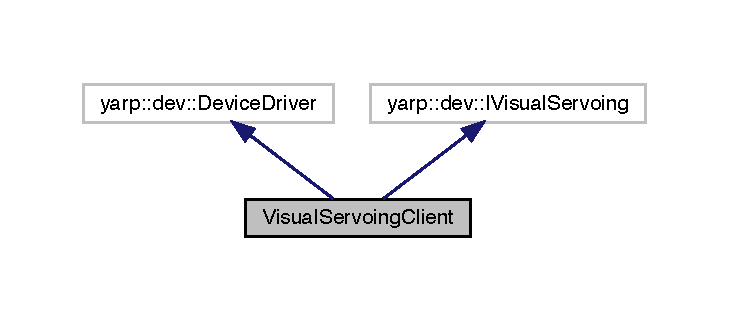
\includegraphics[width=350pt]{classVisualServoingClient__inherit__graph}
\end{center}
\end{figure}
\subsection*{Public Member Functions}
\begin{DoxyCompactItemize}
\item 
\hyperlink{classVisualServoingClient_a8656f6464b80d6a5815232c90bb0f9f7}{Visual\+Servoing\+Client} ()
\item 
\hyperlink{classVisualServoingClient_ab9d97c68e33a3d3aa5bad80921efd45a}{$\sim$\+Visual\+Servoing\+Client} ()
\item 
bool \hyperlink{classVisualServoingClient_ad898a60edcd6dae0b2083db81bf08962}{open} (yarp\+::os\+::\+Searchable \&config) override
\item 
bool \hyperlink{classVisualServoingClient_ac6f08779b3efcb1d5a1b7dc1720c1d6c}{close} () override
\item 
bool \hyperlink{classVisualServoingClient_ae6a66fcc21b354cef0aba9ca6a6192fb}{init\+Facilities} (const bool use\+\_\+direct\+\_\+kin) override
\item 
bool \hyperlink{classVisualServoingClient_a9e0fe7d6cb6cee09c0fb9ed3903a66be}{reset\+Facilities} () override
\item 
bool \hyperlink{classVisualServoingClient_a6086c261684ff994d4daf31a1a7ffd0f}{stop\+Facilities} () override
\item 
bool \hyperlink{classVisualServoingClient_aa83b1b0be446896611b7c7675d716905}{go\+To\+Goal} (const yarp\+::sig\+::\+Vector \&vec\+\_\+x, const yarp\+::sig\+::\+Vector \&vec\+\_\+o) override
\item 
bool \hyperlink{classVisualServoingClient_a986e0195e3e855f9c613af0bcd43e6e2}{go\+To\+Goal} (const std\+::vector$<$ yarp\+::sig\+::\+Vector $>$ \&vec\+\_\+px\+\_\+l, const std\+::vector$<$ yarp\+::sig\+::\+Vector $>$ \&vec\+\_\+px\+\_\+r) override
\item 
bool \hyperlink{classVisualServoingClient_a4b8e26dc7c8afa9b343947894ff214aa}{set\+Modality} (const std\+::string \&mode) override
\item 
bool \hyperlink{classVisualServoingClient_a056ec60c6b8a144708d8aeda34344111}{set\+Visual\+Servo\+Control} (const std\+::string \&control) override
\item 
bool \hyperlink{classVisualServoingClient_ae9ea048d67f2a92b9be08d737e6622a3}{set\+Control\+Point} (const yarp\+::os\+::\+Const\+String \&point) override
\item 
bool \hyperlink{classVisualServoingClient_a4c416452594f40ef8c752b77b79c136f}{get\+Visual\+Servoing\+Info} (yarp\+::os\+::\+Bottle \&info) override
\item 
bool \hyperlink{classVisualServoingClient_a64ac96092017671a9ffc8498fb10e5fa}{set\+Go\+To\+Goal\+Tolerance} (const double tol=15.\+0) override
\item 
bool \hyperlink{classVisualServoingClient_a833cf672981b3a422a0ac41b2845a6c1}{check\+Visual\+Servoing\+Controller} () override
\item 
bool \hyperlink{classVisualServoingClient_aee7dc8c7897bf2ecaf417e9126fd640e}{wait\+Visual\+Servoing\+Done} (const double period=0.\+1, const double timeout=0.\+0) override
\item 
bool \hyperlink{classVisualServoingClient_aad4f96122bd48b7e8aa08673bde3031b}{stop\+Controller} () override
\item 
bool \hyperlink{classVisualServoingClient_a0ed003d4d4905c72a5cb05e5a8224916}{set\+Translation\+Gain} (const double K\+\_\+x\+\_\+1=1.\+0, const double K\+\_\+x\+\_\+2=0.\+25) override
\item 
bool \hyperlink{classVisualServoingClient_acf12ca40f4a4070f8c6ed36b21c0e9e4}{set\+Max\+Translation\+Velocity} (const double max\+\_\+x\+\_\+dot) override
\item 
bool \hyperlink{classVisualServoingClient_a1b8a1af7306d708a56766d69af1a3086}{set\+Translation\+Gain\+Switch\+Tolerance} (const double K\+\_\+x\+\_\+tol=30.\+0) override
\item 
bool \hyperlink{classVisualServoingClient_a3df91c530a6aec77e9fd6d418ba3efaf}{set\+Orientation\+Gain} (const double K\+\_\+o\+\_\+1=1.\+5, const double K\+\_\+o\+\_\+2=0.\+375) override
\item 
bool \hyperlink{classVisualServoingClient_a0caa332fbb62645312593b053d62d02c}{set\+Max\+Orientation\+Velocity} (const double max\+\_\+o\+\_\+dot) override
\item 
bool \hyperlink{classVisualServoingClient_acaa5865c6709780f9c6ea6d31687ac2e}{set\+Orientation\+Gain\+Switch\+Tolerance} (const double K\+\_\+o\+\_\+tol=30.\+0) override
\item 
std\+::vector$<$ yarp\+::sig\+::\+Vector $>$ \hyperlink{classVisualServoingClient_a23fb8539faf13002caa40123dce709a1}{get3\+D\+Goal\+Positions\+From3\+D\+Pose} (const yarp\+::sig\+::\+Vector \&x, const yarp\+::sig\+::\+Vector \&o) override
\item 
std\+::vector$<$ yarp\+::sig\+::\+Vector $>$ \hyperlink{classVisualServoingClient_aa9ede5b1061b05533ac1c8cc7c52183c}{get\+Goal\+Pixels\+From3\+D\+Pose} (const yarp\+::sig\+::\+Vector \&x, const yarp\+::sig\+::\+Vector \&o, const Cam\+Sel \&cam) override
\item 
bool \hyperlink{classVisualServoingClient_a0b7df161daebc8c947c8a29ad7e309ef}{stored\+Init} (const std\+::string \&label) override
\item 
bool \hyperlink{classVisualServoingClient_af1070526a82d7e99bb0dba8a34bc68cf}{stored\+Go\+To\+Goal} (const std\+::string \&label) override
\item 
bool \hyperlink{classVisualServoingClient_ab5c9cf7eb3967b9f28e298ac58f7bb86}{go\+To\+S\+F\+M\+Goal} () override
\end{DoxyCompactItemize}
\subsection*{Private Member Functions}
\begin{DoxyCompactItemize}
\item 
void \hyperlink{classVisualServoingClient_a1a6aee4324f230185356960adc22ecfc}{y\+Info\+Verbose} (const yarp\+::os\+::\+Const\+String \&str) const
\item 
void \hyperlink{classVisualServoingClient_ab9c5c456032851ef0bec5b97980a97f8}{y\+Warning\+Verbose} (const yarp\+::os\+::\+Const\+String \&str) const
\item 
void \hyperlink{classVisualServoingClient_a0977c43fb682f6eefa6ad90850a98ff4}{y\+Error\+Verbose} (const yarp\+::os\+::\+Const\+String \&str) const
\end{DoxyCompactItemize}
\subsection*{Private Attributes}
\begin{DoxyCompactItemize}
\item 
bool \hyperlink{classVisualServoingClient_a8c18353c2a7f838ce75b5a426b5b4c21}{verbosity\+\_\+} = false
\item 
yarp\+::os\+::\+Const\+String \hyperlink{classVisualServoingClient_a0b485c388dfe357bd5b504bc87449ff5}{local\+\_\+} = \char`\"{}\char`\"{}
\item 
yarp\+::os\+::\+Const\+String \hyperlink{classVisualServoingClient_ad2d718343d5fec7dd28c2eff9fd5d481}{remote\+\_\+} = \char`\"{}\char`\"{}
\item 
\hyperlink{classVisualServoingIDL}{Visual\+Servoing\+I\+DL} \hyperlink{classVisualServoingClient_a13c52256db8c843064c7c7ad4fc38e13}{visualservoing\+\_\+control}
\item 
yarp\+::os\+::\+Port \hyperlink{classVisualServoingClient_ae1f44cd6e0759f1d32d581f9d9ea8137}{port\+\_\+rpc\+\_\+command\+\_\+}
\end{DoxyCompactItemize}


\subsection{Detailed Description}


Definition at line 19 of file Visual\+Servoing\+Client.\+h.



\subsection{Constructor \& Destructor Documentation}
\mbox{\Hypertarget{classVisualServoingClient_a8656f6464b80d6a5815232c90bb0f9f7}\label{classVisualServoingClient_a8656f6464b80d6a5815232c90bb0f9f7}} 
\index{Visual\+Servoing\+Client@{Visual\+Servoing\+Client}!Visual\+Servoing\+Client@{Visual\+Servoing\+Client}}
\index{Visual\+Servoing\+Client@{Visual\+Servoing\+Client}!Visual\+Servoing\+Client@{Visual\+Servoing\+Client}}
\subsubsection{\texorpdfstring{Visual\+Servoing\+Client()}{VisualServoingClient()}}
{\footnotesize\ttfamily Visual\+Servoing\+Client\+::\+Visual\+Servoing\+Client (\begin{DoxyParamCaption}{ }\end{DoxyParamCaption})}



Definition at line 21 of file Visual\+Servoing\+Client.\+cpp.

\mbox{\Hypertarget{classVisualServoingClient_ab9d97c68e33a3d3aa5bad80921efd45a}\label{classVisualServoingClient_ab9d97c68e33a3d3aa5bad80921efd45a}} 
\index{Visual\+Servoing\+Client@{Visual\+Servoing\+Client}!````~Visual\+Servoing\+Client@{$\sim$\+Visual\+Servoing\+Client}}
\index{````~Visual\+Servoing\+Client@{$\sim$\+Visual\+Servoing\+Client}!Visual\+Servoing\+Client@{Visual\+Servoing\+Client}}
\subsubsection{\texorpdfstring{$\sim$\+Visual\+Servoing\+Client()}{~VisualServoingClient()}}
{\footnotesize\ttfamily Visual\+Servoing\+Client\+::$\sim$\+Visual\+Servoing\+Client (\begin{DoxyParamCaption}{ }\end{DoxyParamCaption})}



Definition at line 28 of file Visual\+Servoing\+Client.\+cpp.



\subsection{Member Function Documentation}
\mbox{\Hypertarget{classVisualServoingClient_a833cf672981b3a422a0ac41b2845a6c1}\label{classVisualServoingClient_a833cf672981b3a422a0ac41b2845a6c1}} 
\index{Visual\+Servoing\+Client@{Visual\+Servoing\+Client}!check\+Visual\+Servoing\+Controller@{check\+Visual\+Servoing\+Controller}}
\index{check\+Visual\+Servoing\+Controller@{check\+Visual\+Servoing\+Controller}!Visual\+Servoing\+Client@{Visual\+Servoing\+Client}}
\subsubsection{\texorpdfstring{check\+Visual\+Servoing\+Controller()}{checkVisualServoingController()}}
{\footnotesize\ttfamily bool Visual\+Servoing\+Client\+::check\+Visual\+Servoing\+Controller (\begin{DoxyParamCaption}{ }\end{DoxyParamCaption})\hspace{0.3cm}{\ttfamily [override]}}



Definition at line 201 of file Visual\+Servoing\+Client.\+cpp.

\mbox{\Hypertarget{classVisualServoingClient_ac6f08779b3efcb1d5a1b7dc1720c1d6c}\label{classVisualServoingClient_ac6f08779b3efcb1d5a1b7dc1720c1d6c}} 
\index{Visual\+Servoing\+Client@{Visual\+Servoing\+Client}!close@{close}}
\index{close@{close}!Visual\+Servoing\+Client@{Visual\+Servoing\+Client}}
\subsubsection{\texorpdfstring{close()}{close()}}
{\footnotesize\ttfamily bool Visual\+Servoing\+Client\+::close (\begin{DoxyParamCaption}{ }\end{DoxyParamCaption})\hspace{0.3cm}{\ttfamily [override]}}



Definition at line 88 of file Visual\+Servoing\+Client.\+cpp.

\mbox{\Hypertarget{classVisualServoingClient_a23fb8539faf13002caa40123dce709a1}\label{classVisualServoingClient_a23fb8539faf13002caa40123dce709a1}} 
\index{Visual\+Servoing\+Client@{Visual\+Servoing\+Client}!get3\+D\+Goal\+Positions\+From3\+D\+Pose@{get3\+D\+Goal\+Positions\+From3\+D\+Pose}}
\index{get3\+D\+Goal\+Positions\+From3\+D\+Pose@{get3\+D\+Goal\+Positions\+From3\+D\+Pose}!Visual\+Servoing\+Client@{Visual\+Servoing\+Client}}
\subsubsection{\texorpdfstring{get3\+D\+Goal\+Positions\+From3\+D\+Pose()}{get3DGoalPositionsFrom3DPose()}}
{\footnotesize\ttfamily std\+::vector$<$ Vector $>$ Visual\+Servoing\+Client\+::get3\+D\+Goal\+Positions\+From3\+D\+Pose (\begin{DoxyParamCaption}\item[{const yarp\+::sig\+::\+Vector \&}]{x,  }\item[{const yarp\+::sig\+::\+Vector \&}]{o }\end{DoxyParamCaption})\hspace{0.3cm}{\ttfamily [override]}}



Definition at line 255 of file Visual\+Servoing\+Client.\+cpp.

\mbox{\Hypertarget{classVisualServoingClient_aa9ede5b1061b05533ac1c8cc7c52183c}\label{classVisualServoingClient_aa9ede5b1061b05533ac1c8cc7c52183c}} 
\index{Visual\+Servoing\+Client@{Visual\+Servoing\+Client}!get\+Goal\+Pixels\+From3\+D\+Pose@{get\+Goal\+Pixels\+From3\+D\+Pose}}
\index{get\+Goal\+Pixels\+From3\+D\+Pose@{get\+Goal\+Pixels\+From3\+D\+Pose}!Visual\+Servoing\+Client@{Visual\+Servoing\+Client}}
\subsubsection{\texorpdfstring{get\+Goal\+Pixels\+From3\+D\+Pose()}{getGoalPixelsFrom3DPose()}}
{\footnotesize\ttfamily std\+::vector$<$ Vector $>$ Visual\+Servoing\+Client\+::get\+Goal\+Pixels\+From3\+D\+Pose (\begin{DoxyParamCaption}\item[{const yarp\+::sig\+::\+Vector \&}]{x,  }\item[{const yarp\+::sig\+::\+Vector \&}]{o,  }\item[{const Cam\+Sel \&}]{cam }\end{DoxyParamCaption})\hspace{0.3cm}{\ttfamily [override]}}



Definition at line 271 of file Visual\+Servoing\+Client.\+cpp.

\mbox{\Hypertarget{classVisualServoingClient_a4c416452594f40ef8c752b77b79c136f}\label{classVisualServoingClient_a4c416452594f40ef8c752b77b79c136f}} 
\index{Visual\+Servoing\+Client@{Visual\+Servoing\+Client}!get\+Visual\+Servoing\+Info@{get\+Visual\+Servoing\+Info}}
\index{get\+Visual\+Servoing\+Info@{get\+Visual\+Servoing\+Info}!Visual\+Servoing\+Client@{Visual\+Servoing\+Client}}
\subsubsection{\texorpdfstring{get\+Visual\+Servoing\+Info()}{getVisualServoingInfo()}}
{\footnotesize\ttfamily bool Visual\+Servoing\+Client\+::get\+Visual\+Servoing\+Info (\begin{DoxyParamCaption}\item[{yarp\+::os\+::\+Bottle \&}]{info }\end{DoxyParamCaption})\hspace{0.3cm}{\ttfamily [override]}}



Definition at line 187 of file Visual\+Servoing\+Client.\+cpp.

\mbox{\Hypertarget{classVisualServoingClient_aa83b1b0be446896611b7c7675d716905}\label{classVisualServoingClient_aa83b1b0be446896611b7c7675d716905}} 
\index{Visual\+Servoing\+Client@{Visual\+Servoing\+Client}!go\+To\+Goal@{go\+To\+Goal}}
\index{go\+To\+Goal@{go\+To\+Goal}!Visual\+Servoing\+Client@{Visual\+Servoing\+Client}}
\subsubsection{\texorpdfstring{go\+To\+Goal()}{goToGoal()}\hspace{0.1cm}{\footnotesize\ttfamily [1/2]}}
{\footnotesize\ttfamily bool Visual\+Servoing\+Client\+::go\+To\+Goal (\begin{DoxyParamCaption}\item[{const yarp\+::sig\+::\+Vector \&}]{vec\+\_\+x,  }\item[{const yarp\+::sig\+::\+Vector \&}]{vec\+\_\+o }\end{DoxyParamCaption})\hspace{0.3cm}{\ttfamily [override]}}



Referenced by stop\+Facilities().

\mbox{\Hypertarget{classVisualServoingClient_a986e0195e3e855f9c613af0bcd43e6e2}\label{classVisualServoingClient_a986e0195e3e855f9c613af0bcd43e6e2}} 
\index{Visual\+Servoing\+Client@{Visual\+Servoing\+Client}!go\+To\+Goal@{go\+To\+Goal}}
\index{go\+To\+Goal@{go\+To\+Goal}!Visual\+Servoing\+Client@{Visual\+Servoing\+Client}}
\subsubsection{\texorpdfstring{go\+To\+Goal()}{goToGoal()}\hspace{0.1cm}{\footnotesize\ttfamily [2/2]}}
{\footnotesize\ttfamily bool Visual\+Servoing\+Client\+::go\+To\+Goal (\begin{DoxyParamCaption}\item[{const std\+::vector$<$ yarp\+::sig\+::\+Vector $>$ \&}]{vec\+\_\+px\+\_\+l,  }\item[{const std\+::vector$<$ yarp\+::sig\+::\+Vector $>$ \&}]{vec\+\_\+px\+\_\+r }\end{DoxyParamCaption})\hspace{0.3cm}{\ttfamily [override]}}

\mbox{\Hypertarget{classVisualServoingClient_ab5c9cf7eb3967b9f28e298ac58f7bb86}\label{classVisualServoingClient_ab5c9cf7eb3967b9f28e298ac58f7bb86}} 
\index{Visual\+Servoing\+Client@{Visual\+Servoing\+Client}!go\+To\+S\+F\+M\+Goal@{go\+To\+S\+F\+M\+Goal}}
\index{go\+To\+S\+F\+M\+Goal@{go\+To\+S\+F\+M\+Goal}!Visual\+Servoing\+Client@{Visual\+Servoing\+Client}}
\subsubsection{\texorpdfstring{go\+To\+S\+F\+M\+Goal()}{goToSFMGoal()}}
{\footnotesize\ttfamily bool Visual\+Servoing\+Client\+::go\+To\+S\+F\+M\+Goal (\begin{DoxyParamCaption}{ }\end{DoxyParamCaption})\hspace{0.3cm}{\ttfamily [override]}}



Definition at line 299 of file Visual\+Servoing\+Client.\+cpp.

\mbox{\Hypertarget{classVisualServoingClient_ae6a66fcc21b354cef0aba9ca6a6192fb}\label{classVisualServoingClient_ae6a66fcc21b354cef0aba9ca6a6192fb}} 
\index{Visual\+Servoing\+Client@{Visual\+Servoing\+Client}!init\+Facilities@{init\+Facilities}}
\index{init\+Facilities@{init\+Facilities}!Visual\+Servoing\+Client@{Visual\+Servoing\+Client}}
\subsubsection{\texorpdfstring{init\+Facilities()}{initFacilities()}}
{\footnotesize\ttfamily bool Visual\+Servoing\+Client\+::init\+Facilities (\begin{DoxyParamCaption}\item[{const bool}]{use\+\_\+direct\+\_\+kin }\end{DoxyParamCaption})\hspace{0.3cm}{\ttfamily [override]}}



Definition at line 111 of file Visual\+Servoing\+Client.\+cpp.

\mbox{\Hypertarget{classVisualServoingClient_ad898a60edcd6dae0b2083db81bf08962}\label{classVisualServoingClient_ad898a60edcd6dae0b2083db81bf08962}} 
\index{Visual\+Servoing\+Client@{Visual\+Servoing\+Client}!open@{open}}
\index{open@{open}!Visual\+Servoing\+Client@{Visual\+Servoing\+Client}}
\subsubsection{\texorpdfstring{open()}{open()}}
{\footnotesize\ttfamily bool Visual\+Servoing\+Client\+::open (\begin{DoxyParamCaption}\item[{yarp\+::os\+::\+Searchable \&}]{config }\end{DoxyParamCaption})\hspace{0.3cm}{\ttfamily [override]}}



Definition at line 36 of file Visual\+Servoing\+Client.\+cpp.

\mbox{\Hypertarget{classVisualServoingClient_a9e0fe7d6cb6cee09c0fb9ed3903a66be}\label{classVisualServoingClient_a9e0fe7d6cb6cee09c0fb9ed3903a66be}} 
\index{Visual\+Servoing\+Client@{Visual\+Servoing\+Client}!reset\+Facilities@{reset\+Facilities}}
\index{reset\+Facilities@{reset\+Facilities}!Visual\+Servoing\+Client@{Visual\+Servoing\+Client}}
\subsubsection{\texorpdfstring{reset\+Facilities()}{resetFacilities()}}
{\footnotesize\ttfamily bool Visual\+Servoing\+Client\+::reset\+Facilities (\begin{DoxyParamCaption}{ }\end{DoxyParamCaption})\hspace{0.3cm}{\ttfamily [override]}}



Definition at line 117 of file Visual\+Servoing\+Client.\+cpp.

\mbox{\Hypertarget{classVisualServoingClient_ae9ea048d67f2a92b9be08d737e6622a3}\label{classVisualServoingClient_ae9ea048d67f2a92b9be08d737e6622a3}} 
\index{Visual\+Servoing\+Client@{Visual\+Servoing\+Client}!set\+Control\+Point@{set\+Control\+Point}}
\index{set\+Control\+Point@{set\+Control\+Point}!Visual\+Servoing\+Client@{Visual\+Servoing\+Client}}
\subsubsection{\texorpdfstring{set\+Control\+Point()}{setControlPoint()}}
{\footnotesize\ttfamily bool Visual\+Servoing\+Client\+::set\+Control\+Point (\begin{DoxyParamCaption}\item[{const yarp\+::os\+::\+Const\+String \&}]{point }\end{DoxyParamCaption})\hspace{0.3cm}{\ttfamily [override]}}



Definition at line 179 of file Visual\+Servoing\+Client.\+cpp.

\mbox{\Hypertarget{classVisualServoingClient_a64ac96092017671a9ffc8498fb10e5fa}\label{classVisualServoingClient_a64ac96092017671a9ffc8498fb10e5fa}} 
\index{Visual\+Servoing\+Client@{Visual\+Servoing\+Client}!set\+Go\+To\+Goal\+Tolerance@{set\+Go\+To\+Goal\+Tolerance}}
\index{set\+Go\+To\+Goal\+Tolerance@{set\+Go\+To\+Goal\+Tolerance}!Visual\+Servoing\+Client@{Visual\+Servoing\+Client}}
\subsubsection{\texorpdfstring{set\+Go\+To\+Goal\+Tolerance()}{setGoToGoalTolerance()}}
{\footnotesize\ttfamily bool Visual\+Servoing\+Client\+::set\+Go\+To\+Goal\+Tolerance (\begin{DoxyParamCaption}\item[{const double}]{tol = {\ttfamily 15.0} }\end{DoxyParamCaption})\hspace{0.3cm}{\ttfamily [override]}}



Definition at line 195 of file Visual\+Servoing\+Client.\+cpp.

\mbox{\Hypertarget{classVisualServoingClient_a0caa332fbb62645312593b053d62d02c}\label{classVisualServoingClient_a0caa332fbb62645312593b053d62d02c}} 
\index{Visual\+Servoing\+Client@{Visual\+Servoing\+Client}!set\+Max\+Orientation\+Velocity@{set\+Max\+Orientation\+Velocity}}
\index{set\+Max\+Orientation\+Velocity@{set\+Max\+Orientation\+Velocity}!Visual\+Servoing\+Client@{Visual\+Servoing\+Client}}
\subsubsection{\texorpdfstring{set\+Max\+Orientation\+Velocity()}{setMaxOrientationVelocity()}}
{\footnotesize\ttfamily bool Visual\+Servoing\+Client\+::set\+Max\+Orientation\+Velocity (\begin{DoxyParamCaption}\item[{const double}]{max\+\_\+o\+\_\+dot }\end{DoxyParamCaption})\hspace{0.3cm}{\ttfamily [override]}}



Definition at line 243 of file Visual\+Servoing\+Client.\+cpp.

\mbox{\Hypertarget{classVisualServoingClient_acf12ca40f4a4070f8c6ed36b21c0e9e4}\label{classVisualServoingClient_acf12ca40f4a4070f8c6ed36b21c0e9e4}} 
\index{Visual\+Servoing\+Client@{Visual\+Servoing\+Client}!set\+Max\+Translation\+Velocity@{set\+Max\+Translation\+Velocity}}
\index{set\+Max\+Translation\+Velocity@{set\+Max\+Translation\+Velocity}!Visual\+Servoing\+Client@{Visual\+Servoing\+Client}}
\subsubsection{\texorpdfstring{set\+Max\+Translation\+Velocity()}{setMaxTranslationVelocity()}}
{\footnotesize\ttfamily bool Visual\+Servoing\+Client\+::set\+Max\+Translation\+Velocity (\begin{DoxyParamCaption}\item[{const double}]{max\+\_\+x\+\_\+dot }\end{DoxyParamCaption})\hspace{0.3cm}{\ttfamily [override]}}



Definition at line 225 of file Visual\+Servoing\+Client.\+cpp.

\mbox{\Hypertarget{classVisualServoingClient_a4b8e26dc7c8afa9b343947894ff214aa}\label{classVisualServoingClient_a4b8e26dc7c8afa9b343947894ff214aa}} 
\index{Visual\+Servoing\+Client@{Visual\+Servoing\+Client}!set\+Modality@{set\+Modality}}
\index{set\+Modality@{set\+Modality}!Visual\+Servoing\+Client@{Visual\+Servoing\+Client}}
\subsubsection{\texorpdfstring{set\+Modality()}{setModality()}}
{\footnotesize\ttfamily bool Visual\+Servoing\+Client\+::set\+Modality (\begin{DoxyParamCaption}\item[{const std\+::string \&}]{mode }\end{DoxyParamCaption})\hspace{0.3cm}{\ttfamily [override]}}



Definition at line 167 of file Visual\+Servoing\+Client.\+cpp.

\mbox{\Hypertarget{classVisualServoingClient_a3df91c530a6aec77e9fd6d418ba3efaf}\label{classVisualServoingClient_a3df91c530a6aec77e9fd6d418ba3efaf}} 
\index{Visual\+Servoing\+Client@{Visual\+Servoing\+Client}!set\+Orientation\+Gain@{set\+Orientation\+Gain}}
\index{set\+Orientation\+Gain@{set\+Orientation\+Gain}!Visual\+Servoing\+Client@{Visual\+Servoing\+Client}}
\subsubsection{\texorpdfstring{set\+Orientation\+Gain()}{setOrientationGain()}}
{\footnotesize\ttfamily bool Visual\+Servoing\+Client\+::set\+Orientation\+Gain (\begin{DoxyParamCaption}\item[{const double}]{K\+\_\+o\+\_\+1 = {\ttfamily 1.5},  }\item[{const double}]{K\+\_\+o\+\_\+2 = {\ttfamily 0.375} }\end{DoxyParamCaption})\hspace{0.3cm}{\ttfamily [override]}}



Definition at line 237 of file Visual\+Servoing\+Client.\+cpp.

\mbox{\Hypertarget{classVisualServoingClient_acaa5865c6709780f9c6ea6d31687ac2e}\label{classVisualServoingClient_acaa5865c6709780f9c6ea6d31687ac2e}} 
\index{Visual\+Servoing\+Client@{Visual\+Servoing\+Client}!set\+Orientation\+Gain\+Switch\+Tolerance@{set\+Orientation\+Gain\+Switch\+Tolerance}}
\index{set\+Orientation\+Gain\+Switch\+Tolerance@{set\+Orientation\+Gain\+Switch\+Tolerance}!Visual\+Servoing\+Client@{Visual\+Servoing\+Client}}
\subsubsection{\texorpdfstring{set\+Orientation\+Gain\+Switch\+Tolerance()}{setOrientationGainSwitchTolerance()}}
{\footnotesize\ttfamily bool Visual\+Servoing\+Client\+::set\+Orientation\+Gain\+Switch\+Tolerance (\begin{DoxyParamCaption}\item[{const double}]{K\+\_\+o\+\_\+tol = {\ttfamily 30.0} }\end{DoxyParamCaption})\hspace{0.3cm}{\ttfamily [override]}}



Definition at line 249 of file Visual\+Servoing\+Client.\+cpp.

\mbox{\Hypertarget{classVisualServoingClient_a0ed003d4d4905c72a5cb05e5a8224916}\label{classVisualServoingClient_a0ed003d4d4905c72a5cb05e5a8224916}} 
\index{Visual\+Servoing\+Client@{Visual\+Servoing\+Client}!set\+Translation\+Gain@{set\+Translation\+Gain}}
\index{set\+Translation\+Gain@{set\+Translation\+Gain}!Visual\+Servoing\+Client@{Visual\+Servoing\+Client}}
\subsubsection{\texorpdfstring{set\+Translation\+Gain()}{setTranslationGain()}}
{\footnotesize\ttfamily bool Visual\+Servoing\+Client\+::set\+Translation\+Gain (\begin{DoxyParamCaption}\item[{const double}]{K\+\_\+x\+\_\+1 = {\ttfamily 1.0},  }\item[{const double}]{K\+\_\+x\+\_\+2 = {\ttfamily 0.25} }\end{DoxyParamCaption})\hspace{0.3cm}{\ttfamily [override]}}



Definition at line 219 of file Visual\+Servoing\+Client.\+cpp.

\mbox{\Hypertarget{classVisualServoingClient_a1b8a1af7306d708a56766d69af1a3086}\label{classVisualServoingClient_a1b8a1af7306d708a56766d69af1a3086}} 
\index{Visual\+Servoing\+Client@{Visual\+Servoing\+Client}!set\+Translation\+Gain\+Switch\+Tolerance@{set\+Translation\+Gain\+Switch\+Tolerance}}
\index{set\+Translation\+Gain\+Switch\+Tolerance@{set\+Translation\+Gain\+Switch\+Tolerance}!Visual\+Servoing\+Client@{Visual\+Servoing\+Client}}
\subsubsection{\texorpdfstring{set\+Translation\+Gain\+Switch\+Tolerance()}{setTranslationGainSwitchTolerance()}}
{\footnotesize\ttfamily bool Visual\+Servoing\+Client\+::set\+Translation\+Gain\+Switch\+Tolerance (\begin{DoxyParamCaption}\item[{const double}]{K\+\_\+x\+\_\+tol = {\ttfamily 30.0} }\end{DoxyParamCaption})\hspace{0.3cm}{\ttfamily [override]}}



Definition at line 231 of file Visual\+Servoing\+Client.\+cpp.

\mbox{\Hypertarget{classVisualServoingClient_a056ec60c6b8a144708d8aeda34344111}\label{classVisualServoingClient_a056ec60c6b8a144708d8aeda34344111}} 
\index{Visual\+Servoing\+Client@{Visual\+Servoing\+Client}!set\+Visual\+Servo\+Control@{set\+Visual\+Servo\+Control}}
\index{set\+Visual\+Servo\+Control@{set\+Visual\+Servo\+Control}!Visual\+Servoing\+Client@{Visual\+Servoing\+Client}}
\subsubsection{\texorpdfstring{set\+Visual\+Servo\+Control()}{setVisualServoControl()}}
{\footnotesize\ttfamily bool Visual\+Servoing\+Client\+::set\+Visual\+Servo\+Control (\begin{DoxyParamCaption}\item[{const std\+::string \&}]{control }\end{DoxyParamCaption})\hspace{0.3cm}{\ttfamily [override]}}



Definition at line 173 of file Visual\+Servoing\+Client.\+cpp.

\mbox{\Hypertarget{classVisualServoingClient_aad4f96122bd48b7e8aa08673bde3031b}\label{classVisualServoingClient_aad4f96122bd48b7e8aa08673bde3031b}} 
\index{Visual\+Servoing\+Client@{Visual\+Servoing\+Client}!stop\+Controller@{stop\+Controller}}
\index{stop\+Controller@{stop\+Controller}!Visual\+Servoing\+Client@{Visual\+Servoing\+Client}}
\subsubsection{\texorpdfstring{stop\+Controller()}{stopController()}}
{\footnotesize\ttfamily bool Visual\+Servoing\+Client\+::stop\+Controller (\begin{DoxyParamCaption}{ }\end{DoxyParamCaption})\hspace{0.3cm}{\ttfamily [override]}}



Definition at line 213 of file Visual\+Servoing\+Client.\+cpp.

\mbox{\Hypertarget{classVisualServoingClient_a6086c261684ff994d4daf31a1a7ffd0f}\label{classVisualServoingClient_a6086c261684ff994d4daf31a1a7ffd0f}} 
\index{Visual\+Servoing\+Client@{Visual\+Servoing\+Client}!stop\+Facilities@{stop\+Facilities}}
\index{stop\+Facilities@{stop\+Facilities}!Visual\+Servoing\+Client@{Visual\+Servoing\+Client}}
\subsubsection{\texorpdfstring{stop\+Facilities()}{stopFacilities()}}
{\footnotesize\ttfamily bool Visual\+Servoing\+Client\+::stop\+Facilities (\begin{DoxyParamCaption}{ }\end{DoxyParamCaption})\hspace{0.3cm}{\ttfamily [override]}}



Definition at line 123 of file Visual\+Servoing\+Client.\+cpp.



References go\+To\+Goal().

Here is the call graph for this function\+:
\nopagebreak
\begin{figure}[H]
\begin{center}
\leavevmode
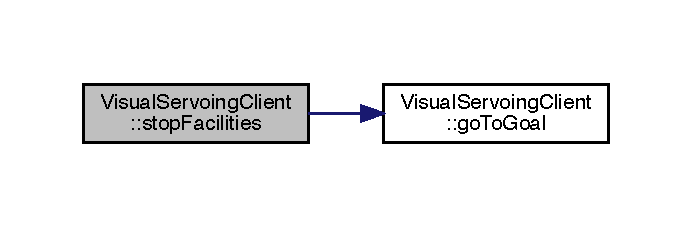
\includegraphics[width=332pt]{classVisualServoingClient_a6086c261684ff994d4daf31a1a7ffd0f_cgraph}
\end{center}
\end{figure}
\mbox{\Hypertarget{classVisualServoingClient_af1070526a82d7e99bb0dba8a34bc68cf}\label{classVisualServoingClient_af1070526a82d7e99bb0dba8a34bc68cf}} 
\index{Visual\+Servoing\+Client@{Visual\+Servoing\+Client}!stored\+Go\+To\+Goal@{stored\+Go\+To\+Goal}}
\index{stored\+Go\+To\+Goal@{stored\+Go\+To\+Goal}!Visual\+Servoing\+Client@{Visual\+Servoing\+Client}}
\subsubsection{\texorpdfstring{stored\+Go\+To\+Goal()}{storedGoToGoal()}}
{\footnotesize\ttfamily bool Visual\+Servoing\+Client\+::stored\+Go\+To\+Goal (\begin{DoxyParamCaption}\item[{const std\+::string \&}]{label }\end{DoxyParamCaption})\hspace{0.3cm}{\ttfamily [override]}}



Definition at line 293 of file Visual\+Servoing\+Client.\+cpp.

\mbox{\Hypertarget{classVisualServoingClient_a0b7df161daebc8c947c8a29ad7e309ef}\label{classVisualServoingClient_a0b7df161daebc8c947c8a29ad7e309ef}} 
\index{Visual\+Servoing\+Client@{Visual\+Servoing\+Client}!stored\+Init@{stored\+Init}}
\index{stored\+Init@{stored\+Init}!Visual\+Servoing\+Client@{Visual\+Servoing\+Client}}
\subsubsection{\texorpdfstring{stored\+Init()}{storedInit()}}
{\footnotesize\ttfamily bool Visual\+Servoing\+Client\+::stored\+Init (\begin{DoxyParamCaption}\item[{const std\+::string \&}]{label }\end{DoxyParamCaption})\hspace{0.3cm}{\ttfamily [override]}}



Definition at line 287 of file Visual\+Servoing\+Client.\+cpp.

\mbox{\Hypertarget{classVisualServoingClient_aee7dc8c7897bf2ecaf417e9126fd640e}\label{classVisualServoingClient_aee7dc8c7897bf2ecaf417e9126fd640e}} 
\index{Visual\+Servoing\+Client@{Visual\+Servoing\+Client}!wait\+Visual\+Servoing\+Done@{wait\+Visual\+Servoing\+Done}}
\index{wait\+Visual\+Servoing\+Done@{wait\+Visual\+Servoing\+Done}!Visual\+Servoing\+Client@{Visual\+Servoing\+Client}}
\subsubsection{\texorpdfstring{wait\+Visual\+Servoing\+Done()}{waitVisualServoingDone()}}
{\footnotesize\ttfamily bool Visual\+Servoing\+Client\+::wait\+Visual\+Servoing\+Done (\begin{DoxyParamCaption}\item[{const double}]{period = {\ttfamily 0.1},  }\item[{const double}]{timeout = {\ttfamily 0.0} }\end{DoxyParamCaption})\hspace{0.3cm}{\ttfamily [override]}}



Definition at line 207 of file Visual\+Servoing\+Client.\+cpp.

\mbox{\Hypertarget{classVisualServoingClient_a0977c43fb682f6eefa6ad90850a98ff4}\label{classVisualServoingClient_a0977c43fb682f6eefa6ad90850a98ff4}} 
\index{Visual\+Servoing\+Client@{Visual\+Servoing\+Client}!y\+Error\+Verbose@{y\+Error\+Verbose}}
\index{y\+Error\+Verbose@{y\+Error\+Verbose}!Visual\+Servoing\+Client@{Visual\+Servoing\+Client}}
\subsubsection{\texorpdfstring{y\+Error\+Verbose()}{yErrorVerbose()}}
{\footnotesize\ttfamily void Visual\+Servoing\+Client\+::y\+Error\+Verbose (\begin{DoxyParamCaption}\item[{const yarp\+::os\+::\+Const\+String \&}]{str }\end{DoxyParamCaption}) const\hspace{0.3cm}{\ttfamily [inline]}, {\ttfamily [private]}}



Definition at line 95 of file Visual\+Servoing\+Client.\+h.

\mbox{\Hypertarget{classVisualServoingClient_a1a6aee4324f230185356960adc22ecfc}\label{classVisualServoingClient_a1a6aee4324f230185356960adc22ecfc}} 
\index{Visual\+Servoing\+Client@{Visual\+Servoing\+Client}!y\+Info\+Verbose@{y\+Info\+Verbose}}
\index{y\+Info\+Verbose@{y\+Info\+Verbose}!Visual\+Servoing\+Client@{Visual\+Servoing\+Client}}
\subsubsection{\texorpdfstring{y\+Info\+Verbose()}{yInfoVerbose()}}
{\footnotesize\ttfamily void Visual\+Servoing\+Client\+::y\+Info\+Verbose (\begin{DoxyParamCaption}\item[{const yarp\+::os\+::\+Const\+String \&}]{str }\end{DoxyParamCaption}) const\hspace{0.3cm}{\ttfamily [inline]}, {\ttfamily [private]}}



Definition at line 93 of file Visual\+Servoing\+Client.\+h.

\mbox{\Hypertarget{classVisualServoingClient_ab9c5c456032851ef0bec5b97980a97f8}\label{classVisualServoingClient_ab9c5c456032851ef0bec5b97980a97f8}} 
\index{Visual\+Servoing\+Client@{Visual\+Servoing\+Client}!y\+Warning\+Verbose@{y\+Warning\+Verbose}}
\index{y\+Warning\+Verbose@{y\+Warning\+Verbose}!Visual\+Servoing\+Client@{Visual\+Servoing\+Client}}
\subsubsection{\texorpdfstring{y\+Warning\+Verbose()}{yWarningVerbose()}}
{\footnotesize\ttfamily void Visual\+Servoing\+Client\+::y\+Warning\+Verbose (\begin{DoxyParamCaption}\item[{const yarp\+::os\+::\+Const\+String \&}]{str }\end{DoxyParamCaption}) const\hspace{0.3cm}{\ttfamily [inline]}, {\ttfamily [private]}}



Definition at line 94 of file Visual\+Servoing\+Client.\+h.



\subsection{Member Data Documentation}
\mbox{\Hypertarget{classVisualServoingClient_a0b485c388dfe357bd5b504bc87449ff5}\label{classVisualServoingClient_a0b485c388dfe357bd5b504bc87449ff5}} 
\index{Visual\+Servoing\+Client@{Visual\+Servoing\+Client}!local\+\_\+@{local\+\_\+}}
\index{local\+\_\+@{local\+\_\+}!Visual\+Servoing\+Client@{Visual\+Servoing\+Client}}
\subsubsection{\texorpdfstring{local\+\_\+}{local\_}}
{\footnotesize\ttfamily yarp\+::os\+::\+Const\+String Visual\+Servoing\+Client\+::local\+\_\+ = \char`\"{}\char`\"{}\hspace{0.3cm}{\ttfamily [private]}}



Definition at line 87 of file Visual\+Servoing\+Client.\+h.

\mbox{\Hypertarget{classVisualServoingClient_ae1f44cd6e0759f1d32d581f9d9ea8137}\label{classVisualServoingClient_ae1f44cd6e0759f1d32d581f9d9ea8137}} 
\index{Visual\+Servoing\+Client@{Visual\+Servoing\+Client}!port\+\_\+rpc\+\_\+command\+\_\+@{port\+\_\+rpc\+\_\+command\+\_\+}}
\index{port\+\_\+rpc\+\_\+command\+\_\+@{port\+\_\+rpc\+\_\+command\+\_\+}!Visual\+Servoing\+Client@{Visual\+Servoing\+Client}}
\subsubsection{\texorpdfstring{port\+\_\+rpc\+\_\+command\+\_\+}{port\_rpc\_command\_}}
{\footnotesize\ttfamily yarp\+::os\+::\+Port Visual\+Servoing\+Client\+::port\+\_\+rpc\+\_\+command\+\_\+\hspace{0.3cm}{\ttfamily [private]}}



Definition at line 91 of file Visual\+Servoing\+Client.\+h.

\mbox{\Hypertarget{classVisualServoingClient_ad2d718343d5fec7dd28c2eff9fd5d481}\label{classVisualServoingClient_ad2d718343d5fec7dd28c2eff9fd5d481}} 
\index{Visual\+Servoing\+Client@{Visual\+Servoing\+Client}!remote\+\_\+@{remote\+\_\+}}
\index{remote\+\_\+@{remote\+\_\+}!Visual\+Servoing\+Client@{Visual\+Servoing\+Client}}
\subsubsection{\texorpdfstring{remote\+\_\+}{remote\_}}
{\footnotesize\ttfamily yarp\+::os\+::\+Const\+String Visual\+Servoing\+Client\+::remote\+\_\+ = \char`\"{}\char`\"{}\hspace{0.3cm}{\ttfamily [private]}}



Definition at line 88 of file Visual\+Servoing\+Client.\+h.

\mbox{\Hypertarget{classVisualServoingClient_a8c18353c2a7f838ce75b5a426b5b4c21}\label{classVisualServoingClient_a8c18353c2a7f838ce75b5a426b5b4c21}} 
\index{Visual\+Servoing\+Client@{Visual\+Servoing\+Client}!verbosity\+\_\+@{verbosity\+\_\+}}
\index{verbosity\+\_\+@{verbosity\+\_\+}!Visual\+Servoing\+Client@{Visual\+Servoing\+Client}}
\subsubsection{\texorpdfstring{verbosity\+\_\+}{verbosity\_}}
{\footnotesize\ttfamily bool Visual\+Servoing\+Client\+::verbosity\+\_\+ = false\hspace{0.3cm}{\ttfamily [private]}}



Definition at line 86 of file Visual\+Servoing\+Client.\+h.

\mbox{\Hypertarget{classVisualServoingClient_a13c52256db8c843064c7c7ad4fc38e13}\label{classVisualServoingClient_a13c52256db8c843064c7c7ad4fc38e13}} 
\index{Visual\+Servoing\+Client@{Visual\+Servoing\+Client}!visualservoing\+\_\+control@{visualservoing\+\_\+control}}
\index{visualservoing\+\_\+control@{visualservoing\+\_\+control}!Visual\+Servoing\+Client@{Visual\+Servoing\+Client}}
\subsubsection{\texorpdfstring{visualservoing\+\_\+control}{visualservoing\_control}}
{\footnotesize\ttfamily \hyperlink{classVisualServoingIDL}{Visual\+Servoing\+I\+DL} Visual\+Servoing\+Client\+::visualservoing\+\_\+control\hspace{0.3cm}{\ttfamily [private]}}



Definition at line 90 of file Visual\+Servoing\+Client.\+h.



The documentation for this class was generated from the following files\+:\begin{DoxyCompactItemize}
\item 
/\+Users/\+Claudio/\+Git\+Hub/visual-\/tracking-\/control/src/visualservoing/visualservoingclient/include/\hyperlink{VisualServoingClient_8h}{Visual\+Servoing\+Client.\+h}\item 
/\+Users/\+Claudio/\+Git\+Hub/visual-\/tracking-\/control/src/visualservoing/visualservoingclient/src/\hyperlink{VisualServoingClient_8cpp}{Visual\+Servoing\+Client.\+cpp}\end{DoxyCompactItemize}

\hypertarget{classVisualServoingIDL}{}\section{Visual\+Servoing\+I\+DL Class Reference}
\label{classVisualServoingIDL}\index{Visual\+Servoing\+I\+DL@{Visual\+Servoing\+I\+DL}}


\hyperlink{classVisualServoingIDL}{Visual\+Servoing\+I\+DL} I\+DL Interface to Server\+Visual\+Servoing functionalities.  




{\ttfamily \#include $<$Visual\+Servoing\+I\+D\+L.\+h$>$}



Inheritance diagram for Visual\+Servoing\+I\+DL\+:
\nopagebreak
\begin{figure}[H]
\begin{center}
\leavevmode
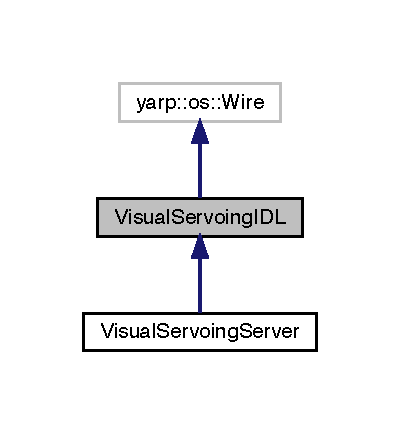
\includegraphics[width=192pt]{classVisualServoingIDL__inherit__graph}
\end{center}
\end{figure}
\subsection*{Public Member Functions}
\begin{DoxyCompactItemize}
\item 
\hyperlink{classVisualServoingIDL_adff6d75dfaede0453d02b6f017e9e977}{Visual\+Servoing\+I\+DL} ()
\item 
virtual bool \hyperlink{classVisualServoingIDL_aae4ee4c07b50956396fd59bbb00fd9c7}{init\+\_\+facilities} (const bool use\+\_\+direct\+\_\+kin)
\begin{DoxyCompactList}\small\item\em Initialize support modules and connections to perform a visual servoing task. \end{DoxyCompactList}\item 
virtual bool \hyperlink{classVisualServoingIDL_a23929f03db99f80426a859cdad68e48c}{reset\+\_\+facilities} ()
\begin{DoxyCompactList}\small\item\em Reset support modules and connections to perform the current initialized visual servoing task. \end{DoxyCompactList}\item 
virtual bool \hyperlink{classVisualServoingIDL_a777cc1a83b3c0ae3dd86e36a0298970e}{stop\+\_\+facilities} ()
\begin{DoxyCompactList}\small\item\em Stop and disconnect support modules and connections used for visual servoing. \end{DoxyCompactList}\item 
virtual bool \hyperlink{classVisualServoingIDL_a75929f915651161c43ed032e9f69a361}{go\+\_\+to\+\_\+px\+\_\+goal} (const std\+::vector$<$ std\+::vector$<$ double $>$ $>$ \&vec\+\_\+px\+\_\+l, const std\+::vector$<$ std\+::vector$<$ double $>$ $>$ \&vec\+\_\+px\+\_\+r)
\begin{DoxyCompactList}\small\item\em Set the goal points on both left and right camera image plane and start visual servoing. \end{DoxyCompactList}\item 
virtual bool \hyperlink{classVisualServoingIDL_a697368ff5a1b3f16069d1d10f25ca888}{go\+\_\+to\+\_\+pose\+\_\+goal} (const std\+::vector$<$ double $>$ \&vec\+\_\+x, const std\+::vector$<$ double $>$ \&vec\+\_\+o)
\begin{DoxyCompactList}\small\item\em Set the goal point (3D for the position + 4D axis-\/angle for the orientation) and start visual servoing. \end{DoxyCompactList}\item 
virtual bool \hyperlink{classVisualServoingIDL_acf88e08e442c512452efe69f103f8f12}{set\+\_\+modality} (const std\+::string \&mode)
\begin{DoxyCompactList}\small\item\em Set visual servoing operating mode between\+: \end{DoxyCompactList}\item 
virtual bool \hyperlink{classVisualServoingIDL_a3db9d27ad8982f561f44a644897c8a9e}{set\+\_\+visual\+\_\+servo\+\_\+control} (const std\+::string \&control)
\begin{DoxyCompactList}\small\item\em Set visual servo control law between\+: \end{DoxyCompactList}\item 
virtual bool \hyperlink{classVisualServoingIDL_a9b84b61f0d80d9c931e1947a5e86c761}{set\+\_\+control\+\_\+point} (const std\+::string \&point)
\begin{DoxyCompactList}\small\item\em Set the point controlled during visual servoing. \end{DoxyCompactList}\item 
virtual std\+::vector$<$ std\+::string $>$ \hyperlink{classVisualServoingIDL_a9654ec3984d53b41f50e0d70b2991203}{get\+\_\+visual\+\_\+servoing\+\_\+info} ()
\begin{DoxyCompactList}\small\item\em Return useful information for visual servoing. \end{DoxyCompactList}\item 
virtual bool \hyperlink{classVisualServoingIDL_aa465471a7300861c1f991f08eb257694}{set\+\_\+go\+\_\+to\+\_\+goal\+\_\+tolerance} (const double tol)
\begin{DoxyCompactList}\small\item\em Set visual servoing goal tolerance. \end{DoxyCompactList}\item 
virtual bool \hyperlink{classVisualServoingIDL_a6426bda1341487c0dbb1f6a048a45deb}{check\+\_\+visual\+\_\+servoing\+\_\+controller} ()
\begin{DoxyCompactList}\small\item\em Check once whether the visual servoing controller is running or not. \end{DoxyCompactList}\item 
virtual bool \hyperlink{classVisualServoingIDL_aa9c9a265e56b0f85c297d2b7d3c8d9c3}{wait\+\_\+visual\+\_\+servoing\+\_\+done} (const double period, const double timeout)
\begin{DoxyCompactList}\small\item\em Wait until visual servoing reaches the goal. \end{DoxyCompactList}\item 
virtual bool \hyperlink{classVisualServoingIDL_ac8909c1f4d5eb4cd1ab010fb3dcd7efb}{stop\+\_\+controller} ()
\begin{DoxyCompactList}\small\item\em Ask for an immediate stop of the visual servoing controller. \end{DoxyCompactList}\item 
virtual bool \hyperlink{classVisualServoingIDL_a49034ed3c3d7b150ea0edb984217af31}{set\+\_\+translation\+\_\+gain} (const double K\+\_\+x\+\_\+1, const double K\+\_\+x\+\_\+2)
\begin{DoxyCompactList}\small\item\em Set the translation gains of the visual servoing control algorithm. \end{DoxyCompactList}\item 
virtual bool \hyperlink{classVisualServoingIDL_af928c1409ad82c6b5fa1aff93ef9d0c4}{set\+\_\+max\+\_\+translation\+\_\+velocity} (const double max\+\_\+x\+\_\+dot)
\begin{DoxyCompactList}\small\item\em Set the maximum translation velocity of the visual servoing control algorithm (same for each axis). \end{DoxyCompactList}\item 
virtual bool \hyperlink{classVisualServoingIDL_ad7800969fdb9a88cce5e59552fca8b1f}{set\+\_\+translation\+\_\+gain\+\_\+switch\+\_\+tolerance} (const double K\+\_\+x\+\_\+tol)
\begin{DoxyCompactList}\small\item\em Set the tolerance, in pixels, at which the translation control law swithces its gain value. \end{DoxyCompactList}\item 
virtual bool \hyperlink{classVisualServoingIDL_a63069a57bf0a190f0d76b5c0eba694fb}{set\+\_\+orientation\+\_\+gain} (const double K\+\_\+o\+\_\+1, const double K\+\_\+o\+\_\+2)
\begin{DoxyCompactList}\small\item\em Set the orientation gains of the visual servoing control algorithm. \end{DoxyCompactList}\item 
virtual bool \hyperlink{classVisualServoingIDL_ad2495422c8f1dda27b85db96c42a7042}{set\+\_\+max\+\_\+orientation\+\_\+velocity} (const double max\+\_\+o\+\_\+dot)
\begin{DoxyCompactList}\small\item\em Set the maximum angular velocity of the axis-\/angle velocity vector of the visual servoing control algorithm. \end{DoxyCompactList}\item 
virtual bool \hyperlink{classVisualServoingIDL_acaf4ad7fa8a2443d4719e3f56b8d72b0}{set\+\_\+orientation\+\_\+gain\+\_\+switch\+\_\+tolerance} (const double K\+\_\+o\+\_\+tol)
\begin{DoxyCompactList}\small\item\em Set the tolerance, in pixels, at which the orientation control law swithces its gain value. \end{DoxyCompactList}\item 
virtual std\+::vector$<$ std\+::vector$<$ double $>$ $>$ \hyperlink{classVisualServoingIDL_a175b2d3fb77000e0012c7a8d16e9a379}{get\+\_\+3\+D\+\_\+goal\+\_\+positions\+\_\+from\+\_\+3\+D\+\_\+pose} (const std\+::vector$<$ double $>$ \&x, const std\+::vector$<$ double $>$ \&o)
\begin{DoxyCompactList}\small\item\em Helper function\+: extract four Cartesian points lying on the plane defined by the frame o in the position x relative to the robot base frame. \end{DoxyCompactList}\item 
virtual std\+::vector$<$ std\+::vector$<$ double $>$ $>$ \hyperlink{classVisualServoingIDL_afb359486a7e42bfda3ddf66a2e518e90}{get\+\_\+goal\+\_\+pixels\+\_\+from\+\_\+3\+D\+\_\+pose} (const std\+::vector$<$ double $>$ \&x, const std\+::vector$<$ double $>$ \&o, const std\+::string \&cam)
\begin{DoxyCompactList}\small\item\em Helper function\+: extract four 2D pixel points lying on the plane defined by the frame o in the position x relative to the robot base frame. \end{DoxyCompactList}\item 
virtual bool \hyperlink{classVisualServoingIDL_a3d5503e1d4bb2b25a11cbd5357b3013b}{quit} ()
\begin{DoxyCompactList}\small\item\em Gently close the visual servoing device, deallocating resources. \end{DoxyCompactList}\item 
virtual bool \hyperlink{classVisualServoingIDL_a20ff1561b87126c9b852eacd5ea59d26}{stored\+\_\+init} (const std\+::string \&label)
\begin{DoxyCompactList}\small\item\em Initialize the robot to an initial position. \end{DoxyCompactList}\item 
virtual bool \hyperlink{classVisualServoingIDL_aa751cf35650259ae7cff331c9d19c694}{stored\+\_\+go\+\_\+to\+\_\+goal} (const std\+::string \&label)
\begin{DoxyCompactList}\small\item\em Set the robot visual servoing goal. \end{DoxyCompactList}\item 
virtual bool \hyperlink{classVisualServoingIDL_aff8af7d3ebe68f5fbfa7197eb7115723}{get\+\_\+goal\+\_\+from\+\_\+sfm} ()
\begin{DoxyCompactList}\small\item\em Get goal point from S\+FM module. \end{DoxyCompactList}\item 
virtual bool \hyperlink{classVisualServoingIDL_a97106bf829447896de03680d78b960a5}{read} (yarp\+::os\+::\+Connection\+Reader \&connection) override
\item 
virtual std\+::vector$<$ std\+::string $>$ \hyperlink{classVisualServoingIDL_a99974ef8858179f14e2762c2d7bf4ed5}{help} (const std\+::string \&function\+Name=\char`\"{}-\/-\/all\char`\"{})
\end{DoxyCompactItemize}


\subsection{Detailed Description}
\hyperlink{classVisualServoingIDL}{Visual\+Servoing\+I\+DL} I\+DL Interface to Server\+Visual\+Servoing functionalities. 

Definition at line 17 of file Visual\+Servoing\+I\+D\+L.\+h.



\subsection{Constructor \& Destructor Documentation}
\mbox{\Hypertarget{classVisualServoingIDL_adff6d75dfaede0453d02b6f017e9e977}\label{classVisualServoingIDL_adff6d75dfaede0453d02b6f017e9e977}} 
\index{Visual\+Servoing\+I\+DL@{Visual\+Servoing\+I\+DL}!Visual\+Servoing\+I\+DL@{Visual\+Servoing\+I\+DL}}
\index{Visual\+Servoing\+I\+DL@{Visual\+Servoing\+I\+DL}!Visual\+Servoing\+I\+DL@{Visual\+Servoing\+I\+DL}}
\subsubsection{\texorpdfstring{Visual\+Servoing\+I\+D\+L()}{VisualServoingIDL()}}
{\footnotesize\ttfamily Visual\+Servoing\+I\+D\+L\+::\+Visual\+Servoing\+I\+DL (\begin{DoxyParamCaption}{ }\end{DoxyParamCaption})}



\subsection{Member Function Documentation}
\mbox{\Hypertarget{classVisualServoingIDL_a6426bda1341487c0dbb1f6a048a45deb}\label{classVisualServoingIDL_a6426bda1341487c0dbb1f6a048a45deb}} 
\index{Visual\+Servoing\+I\+DL@{Visual\+Servoing\+I\+DL}!check\+\_\+visual\+\_\+servoing\+\_\+controller@{check\+\_\+visual\+\_\+servoing\+\_\+controller}}
\index{check\+\_\+visual\+\_\+servoing\+\_\+controller@{check\+\_\+visual\+\_\+servoing\+\_\+controller}!Visual\+Servoing\+I\+DL@{Visual\+Servoing\+I\+DL}}
\subsubsection{\texorpdfstring{check\+\_\+visual\+\_\+servoing\+\_\+controller()}{check\_visual\_servoing\_controller()}}
{\footnotesize\ttfamily virtual bool Visual\+Servoing\+I\+D\+L\+::check\+\_\+visual\+\_\+servoing\+\_\+controller (\begin{DoxyParamCaption}{ }\end{DoxyParamCaption})\hspace{0.3cm}{\ttfamily [virtual]}}



Check once whether the visual servoing controller is running or not. 

\begin{DoxyReturn}{Returns}
true/false on it is running/not running. 
\end{DoxyReturn}
\begin{DoxyNote}{Note}
The visual servoing controller may be terminated due to many different reasons, not strictly related to reaching the goal. 
\end{DoxyNote}


Reimplemented in \hyperlink{classVisualServoingServer_a17a9b2913815c52b5a1bd2fd84d9f18e}{Visual\+Servoing\+Server}.

\mbox{\Hypertarget{classVisualServoingIDL_a175b2d3fb77000e0012c7a8d16e9a379}\label{classVisualServoingIDL_a175b2d3fb77000e0012c7a8d16e9a379}} 
\index{Visual\+Servoing\+I\+DL@{Visual\+Servoing\+I\+DL}!get\+\_\+3\+D\+\_\+goal\+\_\+positions\+\_\+from\+\_\+3\+D\+\_\+pose@{get\+\_\+3\+D\+\_\+goal\+\_\+positions\+\_\+from\+\_\+3\+D\+\_\+pose}}
\index{get\+\_\+3\+D\+\_\+goal\+\_\+positions\+\_\+from\+\_\+3\+D\+\_\+pose@{get\+\_\+3\+D\+\_\+goal\+\_\+positions\+\_\+from\+\_\+3\+D\+\_\+pose}!Visual\+Servoing\+I\+DL@{Visual\+Servoing\+I\+DL}}
\subsubsection{\texorpdfstring{get\+\_\+3\+D\+\_\+goal\+\_\+positions\+\_\+from\+\_\+3\+D\+\_\+pose()}{get\_3D\_goal\_positions\_from\_3D\_pose()}}
{\footnotesize\ttfamily virtual std\+::vector$<$std\+::vector$<$double$>$ $>$ Visual\+Servoing\+I\+D\+L\+::get\+\_\+3\+D\+\_\+goal\+\_\+positions\+\_\+from\+\_\+3\+D\+\_\+pose (\begin{DoxyParamCaption}\item[{const std\+::vector$<$ double $>$ \&}]{x,  }\item[{const std\+::vector$<$ double $>$ \&}]{o }\end{DoxyParamCaption})\hspace{0.3cm}{\ttfamily [virtual]}}



Helper function\+: extract four Cartesian points lying on the plane defined by the frame o in the position x relative to the robot base frame. 


\begin{DoxyParams}{Parameters}
{\em x} & a 3D vector which is filled with the actual position (x, y, z) \mbox{[}m\mbox{]}. \\
\hline
{\em o} & a 4D vector which is filled with the actual orientation using axis-\/angle representation (xa, ya, za) and (theta) \mbox{[}rad\mbox{]}. \\
\hline
\end{DoxyParams}
\begin{DoxyReturn}{Returns}
on success\+: a collection of four Cartesian points (position only) extracted from the plane defined by x and o; on failure\+: an empty list. 
\end{DoxyReturn}
\begin{DoxyNote}{Note}
It is always suggested to check whether the returned list is empty or not and to take proper counter actions. 
\end{DoxyNote}


Reimplemented in \hyperlink{classVisualServoingServer_a542e0a6bf6158563a601740363911474}{Visual\+Servoing\+Server}.

\mbox{\Hypertarget{classVisualServoingIDL_aff8af7d3ebe68f5fbfa7197eb7115723}\label{classVisualServoingIDL_aff8af7d3ebe68f5fbfa7197eb7115723}} 
\index{Visual\+Servoing\+I\+DL@{Visual\+Servoing\+I\+DL}!get\+\_\+goal\+\_\+from\+\_\+sfm@{get\+\_\+goal\+\_\+from\+\_\+sfm}}
\index{get\+\_\+goal\+\_\+from\+\_\+sfm@{get\+\_\+goal\+\_\+from\+\_\+sfm}!Visual\+Servoing\+I\+DL@{Visual\+Servoing\+I\+DL}}
\subsubsection{\texorpdfstring{get\+\_\+goal\+\_\+from\+\_\+sfm()}{get\_goal\_from\_sfm()}}
{\footnotesize\ttfamily virtual bool Visual\+Servoing\+I\+D\+L\+::get\+\_\+goal\+\_\+from\+\_\+sfm (\begin{DoxyParamCaption}{ }\end{DoxyParamCaption})\hspace{0.3cm}{\ttfamily [virtual]}}



Get goal point from S\+FM module. 

The point is taken by clicking on a dedicated \textquotesingle{}yarpview\textquotesingle{} G\+UI and the orientation is hard-\/coded. \begin{DoxyNote}{Note}
This service is experimental and should be used with care. 
\end{DoxyNote}
\begin{DoxyReturn}{Returns}
true upon success, false otherwise. 
\end{DoxyReturn}


Reimplemented in \hyperlink{classVisualServoingServer_a3b0e5078c2f32493a2ef31ea32450d80}{Visual\+Servoing\+Server}.

\mbox{\Hypertarget{classVisualServoingIDL_afb359486a7e42bfda3ddf66a2e518e90}\label{classVisualServoingIDL_afb359486a7e42bfda3ddf66a2e518e90}} 
\index{Visual\+Servoing\+I\+DL@{Visual\+Servoing\+I\+DL}!get\+\_\+goal\+\_\+pixels\+\_\+from\+\_\+3\+D\+\_\+pose@{get\+\_\+goal\+\_\+pixels\+\_\+from\+\_\+3\+D\+\_\+pose}}
\index{get\+\_\+goal\+\_\+pixels\+\_\+from\+\_\+3\+D\+\_\+pose@{get\+\_\+goal\+\_\+pixels\+\_\+from\+\_\+3\+D\+\_\+pose}!Visual\+Servoing\+I\+DL@{Visual\+Servoing\+I\+DL}}
\subsubsection{\texorpdfstring{get\+\_\+goal\+\_\+pixels\+\_\+from\+\_\+3\+D\+\_\+pose()}{get\_goal\_pixels\_from\_3D\_pose()}}
{\footnotesize\ttfamily virtual std\+::vector$<$std\+::vector$<$double$>$ $>$ Visual\+Servoing\+I\+D\+L\+::get\+\_\+goal\+\_\+pixels\+\_\+from\+\_\+3\+D\+\_\+pose (\begin{DoxyParamCaption}\item[{const std\+::vector$<$ double $>$ \&}]{x,  }\item[{const std\+::vector$<$ double $>$ \&}]{o,  }\item[{const std\+::string \&}]{cam }\end{DoxyParamCaption})\hspace{0.3cm}{\ttfamily [virtual]}}



Helper function\+: extract four 2D pixel points lying on the plane defined by the frame o in the position x relative to the robot base frame. 


\begin{DoxyParams}{Parameters}
{\em x} & a 3D vector which is filled with the actual position (x, y, z) \mbox{[}m\mbox{]}. \\
\hline
{\em o} & a 4D vector which is filled with the actual orientation using axis-\/angle representation (xa, ya, za) and (theta) \mbox{[}m\mbox{]}/\mbox{[}rad\mbox{]}. \\
\hline
{\em cam} & either \char`\"{}left\char`\"{} or \char`\"{}right\char`\"{} to select left or right camera. \\
\hline
\end{DoxyParams}
\begin{DoxyReturn}{Returns}
on success\+: a collection of three (u, v) pixel points extracted from the plane defined by x and o; on failure\+: an empty list. 
\end{DoxyReturn}
\begin{DoxyNote}{Note}
It is always suggested to check whether the returned list is empty or not and to take proper counter actions. 
\end{DoxyNote}


Reimplemented in \hyperlink{classVisualServoingServer_aaa84d7964120ee1056f422dc2d5eb070}{Visual\+Servoing\+Server}.

\mbox{\Hypertarget{classVisualServoingIDL_a9654ec3984d53b41f50e0d70b2991203}\label{classVisualServoingIDL_a9654ec3984d53b41f50e0d70b2991203}} 
\index{Visual\+Servoing\+I\+DL@{Visual\+Servoing\+I\+DL}!get\+\_\+visual\+\_\+servoing\+\_\+info@{get\+\_\+visual\+\_\+servoing\+\_\+info}}
\index{get\+\_\+visual\+\_\+servoing\+\_\+info@{get\+\_\+visual\+\_\+servoing\+\_\+info}!Visual\+Servoing\+I\+DL@{Visual\+Servoing\+I\+DL}}
\subsubsection{\texorpdfstring{get\+\_\+visual\+\_\+servoing\+\_\+info()}{get\_visual\_servoing\_info()}}
{\footnotesize\ttfamily virtual std\+::vector$<$std\+::string$>$ Visual\+Servoing\+I\+D\+L\+::get\+\_\+visual\+\_\+servoing\+\_\+info (\begin{DoxyParamCaption}{ }\end{DoxyParamCaption})\hspace{0.3cm}{\ttfamily [virtual]}}



Return useful information for visual servoing. 

\begin{DoxyReturn}{Returns}
All the visual servoing information. 
\end{DoxyReturn}


Reimplemented in \hyperlink{classVisualServoingServer_af085e2c5d4c4cfe940b3564b4ba69af6}{Visual\+Servoing\+Server}.

\mbox{\Hypertarget{classVisualServoingIDL_a697368ff5a1b3f16069d1d10f25ca888}\label{classVisualServoingIDL_a697368ff5a1b3f16069d1d10f25ca888}} 
\index{Visual\+Servoing\+I\+DL@{Visual\+Servoing\+I\+DL}!go\+\_\+to\+\_\+pose\+\_\+goal@{go\+\_\+to\+\_\+pose\+\_\+goal}}
\index{go\+\_\+to\+\_\+pose\+\_\+goal@{go\+\_\+to\+\_\+pose\+\_\+goal}!Visual\+Servoing\+I\+DL@{Visual\+Servoing\+I\+DL}}
\subsubsection{\texorpdfstring{go\+\_\+to\+\_\+pose\+\_\+goal()}{go\_to\_pose\_goal()}}
{\footnotesize\ttfamily virtual bool Visual\+Servoing\+I\+D\+L\+::go\+\_\+to\+\_\+pose\+\_\+goal (\begin{DoxyParamCaption}\item[{const std\+::vector$<$ double $>$ \&}]{vec\+\_\+x,  }\item[{const std\+::vector$<$ double $>$ \&}]{vec\+\_\+o }\end{DoxyParamCaption})\hspace{0.3cm}{\ttfamily [virtual]}}



Set the goal point (3D for the position + 4D axis-\/angle for the orientation) and start visual servoing. 


\begin{DoxyParams}{Parameters}
{\em vec\+\_\+x} & a 3D vector which contains the (x, y, z) Cartesian coordinates of the goal. \\
\hline
{\em vec\+\_\+o} & a 4D vector which contains the (x, y, z) axis and theta angle of rotation of the goal. \\
\hline
\end{DoxyParams}
\begin{DoxyNote}{Note}
By invoking this method, the visual servoing goal will be reached in position and orientation together with two parallel tasks. 
\end{DoxyNote}
\begin{DoxyReturn}{Returns}
true/false on success/failure. 
\end{DoxyReturn}


Reimplemented in \hyperlink{classVisualServoingServer_a77f26ac40c67d7a9b7e4ad7840532681}{Visual\+Servoing\+Server}.

\mbox{\Hypertarget{classVisualServoingIDL_a75929f915651161c43ed032e9f69a361}\label{classVisualServoingIDL_a75929f915651161c43ed032e9f69a361}} 
\index{Visual\+Servoing\+I\+DL@{Visual\+Servoing\+I\+DL}!go\+\_\+to\+\_\+px\+\_\+goal@{go\+\_\+to\+\_\+px\+\_\+goal}}
\index{go\+\_\+to\+\_\+px\+\_\+goal@{go\+\_\+to\+\_\+px\+\_\+goal}!Visual\+Servoing\+I\+DL@{Visual\+Servoing\+I\+DL}}
\subsubsection{\texorpdfstring{go\+\_\+to\+\_\+px\+\_\+goal()}{go\_to\_px\_goal()}}
{\footnotesize\ttfamily virtual bool Visual\+Servoing\+I\+D\+L\+::go\+\_\+to\+\_\+px\+\_\+goal (\begin{DoxyParamCaption}\item[{const std\+::vector$<$ std\+::vector$<$ double $>$ $>$ \&}]{vec\+\_\+px\+\_\+l,  }\item[{const std\+::vector$<$ std\+::vector$<$ double $>$ $>$ \&}]{vec\+\_\+px\+\_\+r }\end{DoxyParamCaption})\hspace{0.3cm}{\ttfamily [virtual]}}



Set the goal points on both left and right camera image plane and start visual servoing. 


\begin{DoxyParams}{Parameters}
{\em vec\+\_\+px\+\_\+l} & a collection of four 2D vectors which contains the (u, v) coordinates of the pixels within the left image plane. \\
\hline
{\em vec\+\_\+px\+\_\+r} & a collection of four 2D vectors which contains the (u, v) coordinates of the pixels within the right image plane. \\
\hline
\end{DoxyParams}
\begin{DoxyNote}{Note}
By invoking this method, the visual servoing goal will be reached in orientation first, then in position. This is because there may not be a feasible position solution for every possible orientation. 
\end{DoxyNote}
\begin{DoxyReturn}{Returns}
true/false on success/failure. 
\end{DoxyReturn}
\mbox{\Hypertarget{classVisualServoingIDL_a99974ef8858179f14e2762c2d7bf4ed5}\label{classVisualServoingIDL_a99974ef8858179f14e2762c2d7bf4ed5}} 
\index{Visual\+Servoing\+I\+DL@{Visual\+Servoing\+I\+DL}!help@{help}}
\index{help@{help}!Visual\+Servoing\+I\+DL@{Visual\+Servoing\+I\+DL}}
\subsubsection{\texorpdfstring{help()}{help()}}
{\footnotesize\ttfamily virtual std\+::vector$<$std\+::string$>$ Visual\+Servoing\+I\+D\+L\+::help (\begin{DoxyParamCaption}\item[{const std\+::string \&}]{function\+Name = {\ttfamily \char`\"{}-\/-\/all\char`\"{}} }\end{DoxyParamCaption})\hspace{0.3cm}{\ttfamily [virtual]}}

\mbox{\Hypertarget{classVisualServoingIDL_aae4ee4c07b50956396fd59bbb00fd9c7}\label{classVisualServoingIDL_aae4ee4c07b50956396fd59bbb00fd9c7}} 
\index{Visual\+Servoing\+I\+DL@{Visual\+Servoing\+I\+DL}!init\+\_\+facilities@{init\+\_\+facilities}}
\index{init\+\_\+facilities@{init\+\_\+facilities}!Visual\+Servoing\+I\+DL@{Visual\+Servoing\+I\+DL}}
\subsubsection{\texorpdfstring{init\+\_\+facilities()}{init\_facilities()}}
{\footnotesize\ttfamily virtual bool Visual\+Servoing\+I\+D\+L\+::init\+\_\+facilities (\begin{DoxyParamCaption}\item[{const bool}]{use\+\_\+direct\+\_\+kin }\end{DoxyParamCaption})\hspace{0.3cm}{\ttfamily [virtual]}}



Initialize support modules and connections to perform a visual servoing task. 

This method must be called before any other visual servoing methods. Returns upon successful or failure setup. 
\begin{DoxyParams}{Parameters}
{\em use\+\_\+direct\+\_\+kin} & instruct the visual servoing control to either use direct kinematic or an estimated/refined pose of the end-\/effector. \\
\hline
\end{DoxyParams}
\begin{DoxyNote}{Note}
Default value\+: false. There usually is an error in the robot direct kinematics that should be compensated to perform precise visual servoing. To this end, a recursive Bayesian estimation filter is used to compensate for this error. Such filter is initialized during initialization execution. 
\end{DoxyNote}
\begin{DoxyReturn}{Returns}
true/false on success/failure. 
\end{DoxyReturn}


Reimplemented in \hyperlink{classVisualServoingServer_ad3668e0fc8818f9d2827bbc50087d353}{Visual\+Servoing\+Server}.

\mbox{\Hypertarget{classVisualServoingIDL_a3d5503e1d4bb2b25a11cbd5357b3013b}\label{classVisualServoingIDL_a3d5503e1d4bb2b25a11cbd5357b3013b}} 
\index{Visual\+Servoing\+I\+DL@{Visual\+Servoing\+I\+DL}!quit@{quit}}
\index{quit@{quit}!Visual\+Servoing\+I\+DL@{Visual\+Servoing\+I\+DL}}
\subsubsection{\texorpdfstring{quit()}{quit()}}
{\footnotesize\ttfamily virtual bool Visual\+Servoing\+I\+D\+L\+::quit (\begin{DoxyParamCaption}{ }\end{DoxyParamCaption})\hspace{0.3cm}{\ttfamily [virtual]}}



Gently close the visual servoing device, deallocating resources. 



Reimplemented in \hyperlink{classVisualServoingServer_ac438c7abfb838df458f85e250ead3222}{Visual\+Servoing\+Server}.

\mbox{\Hypertarget{classVisualServoingIDL_a97106bf829447896de03680d78b960a5}\label{classVisualServoingIDL_a97106bf829447896de03680d78b960a5}} 
\index{Visual\+Servoing\+I\+DL@{Visual\+Servoing\+I\+DL}!read@{read}}
\index{read@{read}!Visual\+Servoing\+I\+DL@{Visual\+Servoing\+I\+DL}}
\subsubsection{\texorpdfstring{read()}{read()}}
{\footnotesize\ttfamily virtual bool Visual\+Servoing\+I\+D\+L\+::read (\begin{DoxyParamCaption}\item[{yarp\+::os\+::\+Connection\+Reader \&}]{connection }\end{DoxyParamCaption})\hspace{0.3cm}{\ttfamily [override]}, {\ttfamily [virtual]}}

\mbox{\Hypertarget{classVisualServoingIDL_a23929f03db99f80426a859cdad68e48c}\label{classVisualServoingIDL_a23929f03db99f80426a859cdad68e48c}} 
\index{Visual\+Servoing\+I\+DL@{Visual\+Servoing\+I\+DL}!reset\+\_\+facilities@{reset\+\_\+facilities}}
\index{reset\+\_\+facilities@{reset\+\_\+facilities}!Visual\+Servoing\+I\+DL@{Visual\+Servoing\+I\+DL}}
\subsubsection{\texorpdfstring{reset\+\_\+facilities()}{reset\_facilities()}}
{\footnotesize\ttfamily virtual bool Visual\+Servoing\+I\+D\+L\+::reset\+\_\+facilities (\begin{DoxyParamCaption}{ }\end{DoxyParamCaption})\hspace{0.3cm}{\ttfamily [virtual]}}



Reset support modules and connections to perform the current initialized visual servoing task. 

Returns upon successful or failure setup. \begin{DoxyNote}{Note}
This method also resets the recursive Bayesian estimation filter. It may happen that the recursive Bayesian filter does not provide satisfactory pose estimation or diverges. Thus this method can be used to reset the filter. 
\end{DoxyNote}
\begin{DoxyReturn}{Returns}
true/false on success/failure. 
\end{DoxyReturn}


Reimplemented in \hyperlink{classVisualServoingServer_ae397fa9823f425fccf2837122629383f}{Visual\+Servoing\+Server}.

\mbox{\Hypertarget{classVisualServoingIDL_a9b84b61f0d80d9c931e1947a5e86c761}\label{classVisualServoingIDL_a9b84b61f0d80d9c931e1947a5e86c761}} 
\index{Visual\+Servoing\+I\+DL@{Visual\+Servoing\+I\+DL}!set\+\_\+control\+\_\+point@{set\+\_\+control\+\_\+point}}
\index{set\+\_\+control\+\_\+point@{set\+\_\+control\+\_\+point}!Visual\+Servoing\+I\+DL@{Visual\+Servoing\+I\+DL}}
\subsubsection{\texorpdfstring{set\+\_\+control\+\_\+point()}{set\_control\_point()}}
{\footnotesize\ttfamily virtual bool Visual\+Servoing\+I\+D\+L\+::set\+\_\+control\+\_\+point (\begin{DoxyParamCaption}\item[{const std\+::string \&}]{point }\end{DoxyParamCaption})\hspace{0.3cm}{\ttfamily [virtual]}}



Set the point controlled during visual servoing. 


\begin{DoxyParams}{Parameters}
{\em point} & label of the point to control. \\
\hline
\end{DoxyParams}
\begin{DoxyReturn}{Returns}
true/false on success/failure. 
\end{DoxyReturn}
\begin{DoxyNote}{Note}
The points available to control are identified by a distinct, unique label. Such labels can are stored in the bottle returned by the get\+Info() method. 
\end{DoxyNote}


Reimplemented in \hyperlink{classVisualServoingServer_a4a20a08fec9cfa4765e1245cfce5f9a8}{Visual\+Servoing\+Server}.

\mbox{\Hypertarget{classVisualServoingIDL_aa465471a7300861c1f991f08eb257694}\label{classVisualServoingIDL_aa465471a7300861c1f991f08eb257694}} 
\index{Visual\+Servoing\+I\+DL@{Visual\+Servoing\+I\+DL}!set\+\_\+go\+\_\+to\+\_\+goal\+\_\+tolerance@{set\+\_\+go\+\_\+to\+\_\+goal\+\_\+tolerance}}
\index{set\+\_\+go\+\_\+to\+\_\+goal\+\_\+tolerance@{set\+\_\+go\+\_\+to\+\_\+goal\+\_\+tolerance}!Visual\+Servoing\+I\+DL@{Visual\+Servoing\+I\+DL}}
\subsubsection{\texorpdfstring{set\+\_\+go\+\_\+to\+\_\+goal\+\_\+tolerance()}{set\_go\_to\_goal\_tolerance()}}
{\footnotesize\ttfamily virtual bool Visual\+Servoing\+I\+D\+L\+::set\+\_\+go\+\_\+to\+\_\+goal\+\_\+tolerance (\begin{DoxyParamCaption}\item[{const double}]{tol }\end{DoxyParamCaption})\hspace{0.3cm}{\ttfamily [virtual]}}



Set visual servoing goal tolerance. 


\begin{DoxyParams}{Parameters}
{\em tol} & the tolerance in pixel. \\
\hline
\end{DoxyParams}
\begin{DoxyReturn}{Returns}
true/false on success/failure. 
\end{DoxyReturn}
\begin{DoxyNote}{Note}
Default value\+: 15.\+0 \mbox{[}pixel\mbox{]}. 
\end{DoxyNote}


Reimplemented in \hyperlink{classVisualServoingServer_a0efdb8edb2e4b91dc3168b5051b27f56}{Visual\+Servoing\+Server}.

\mbox{\Hypertarget{classVisualServoingIDL_ad2495422c8f1dda27b85db96c42a7042}\label{classVisualServoingIDL_ad2495422c8f1dda27b85db96c42a7042}} 
\index{Visual\+Servoing\+I\+DL@{Visual\+Servoing\+I\+DL}!set\+\_\+max\+\_\+orientation\+\_\+velocity@{set\+\_\+max\+\_\+orientation\+\_\+velocity}}
\index{set\+\_\+max\+\_\+orientation\+\_\+velocity@{set\+\_\+max\+\_\+orientation\+\_\+velocity}!Visual\+Servoing\+I\+DL@{Visual\+Servoing\+I\+DL}}
\subsubsection{\texorpdfstring{set\+\_\+max\+\_\+orientation\+\_\+velocity()}{set\_max\_orientation\_velocity()}}
{\footnotesize\ttfamily virtual bool Visual\+Servoing\+I\+D\+L\+::set\+\_\+max\+\_\+orientation\+\_\+velocity (\begin{DoxyParamCaption}\item[{const double}]{max\+\_\+o\+\_\+dot }\end{DoxyParamCaption})\hspace{0.3cm}{\ttfamily [virtual]}}



Set the maximum angular velocity of the axis-\/angle velocity vector of the visual servoing control algorithm. 


\begin{DoxyParams}{Parameters}
{\em max\+\_\+x\+\_\+dot} & the maximum allowed angular velocity \mbox{[}rad/s\mbox{]}. \\
\hline
\end{DoxyParams}
\begin{DoxyReturn}{Returns}
true/false on success/failure. 
\end{DoxyReturn}
\begin{DoxyNote}{Note}
Default value\+: 5 $\ast$ (PI / 180.\+0) \mbox{[}rad/s\mbox{]}. 
\end{DoxyNote}


Reimplemented in \hyperlink{classVisualServoingServer_aa3226ef2de2c1743e67788d1bff60679}{Visual\+Servoing\+Server}.

\mbox{\Hypertarget{classVisualServoingIDL_af928c1409ad82c6b5fa1aff93ef9d0c4}\label{classVisualServoingIDL_af928c1409ad82c6b5fa1aff93ef9d0c4}} 
\index{Visual\+Servoing\+I\+DL@{Visual\+Servoing\+I\+DL}!set\+\_\+max\+\_\+translation\+\_\+velocity@{set\+\_\+max\+\_\+translation\+\_\+velocity}}
\index{set\+\_\+max\+\_\+translation\+\_\+velocity@{set\+\_\+max\+\_\+translation\+\_\+velocity}!Visual\+Servoing\+I\+DL@{Visual\+Servoing\+I\+DL}}
\subsubsection{\texorpdfstring{set\+\_\+max\+\_\+translation\+\_\+velocity()}{set\_max\_translation\_velocity()}}
{\footnotesize\ttfamily virtual bool Visual\+Servoing\+I\+D\+L\+::set\+\_\+max\+\_\+translation\+\_\+velocity (\begin{DoxyParamCaption}\item[{const double}]{max\+\_\+x\+\_\+dot }\end{DoxyParamCaption})\hspace{0.3cm}{\ttfamily [virtual]}}



Set the maximum translation velocity of the visual servoing control algorithm (same for each axis). 


\begin{DoxyParams}{Parameters}
{\em max\+\_\+x\+\_\+dot} & the maximum allowed velocity for x, y, z coordinates \mbox{[}m/s\mbox{]}. \\
\hline
\end{DoxyParams}
\begin{DoxyReturn}{Returns}
true/false on success/failure. 
\end{DoxyReturn}
\begin{DoxyNote}{Note}
Default value\+: max\+\_\+x\+\_\+dot = 0.\+025 \mbox{[}m/s\mbox{]}. 
\end{DoxyNote}


Reimplemented in \hyperlink{classVisualServoingServer_a393d1a1d1a7a68fc2098a7c7e8724cc9}{Visual\+Servoing\+Server}.

\mbox{\Hypertarget{classVisualServoingIDL_acf88e08e442c512452efe69f103f8f12}\label{classVisualServoingIDL_acf88e08e442c512452efe69f103f8f12}} 
\index{Visual\+Servoing\+I\+DL@{Visual\+Servoing\+I\+DL}!set\+\_\+modality@{set\+\_\+modality}}
\index{set\+\_\+modality@{set\+\_\+modality}!Visual\+Servoing\+I\+DL@{Visual\+Servoing\+I\+DL}}
\subsubsection{\texorpdfstring{set\+\_\+modality()}{set\_modality()}}
{\footnotesize\ttfamily virtual bool Visual\+Servoing\+I\+D\+L\+::set\+\_\+modality (\begin{DoxyParamCaption}\item[{const std\+::string \&}]{mode }\end{DoxyParamCaption})\hspace{0.3cm}{\ttfamily [virtual]}}



Set visual servoing operating mode between\+: 


\begin{DoxyEnumerate}
\item \textquotesingle{}position\textquotesingle{}\+: position-\/only visual servo control;
\item \textquotesingle{}orientation\textquotesingle{}\+: orientation-\/only visual servo control;
\item \textquotesingle{}pose\textquotesingle{}\+: position + orientation visual servo control. 
\begin{DoxyParams}{Parameters}
{\em mode} & a label referring to one of the three operating mode, i.\+e. \textquotesingle{}position\textquotesingle{}, \textquotesingle{}orientation\textquotesingle{} or \textquotesingle{}pose\textquotesingle{}. \\
\hline
\end{DoxyParams}
\begin{DoxyReturn}{Returns}
true/false on success/failure. 
\end{DoxyReturn}

\end{DoxyEnumerate}

Reimplemented in \hyperlink{classVisualServoingServer_a6d9ec4489caebf0a52b2e5ee149aeb6d}{Visual\+Servoing\+Server}.

\mbox{\Hypertarget{classVisualServoingIDL_a63069a57bf0a190f0d76b5c0eba694fb}\label{classVisualServoingIDL_a63069a57bf0a190f0d76b5c0eba694fb}} 
\index{Visual\+Servoing\+I\+DL@{Visual\+Servoing\+I\+DL}!set\+\_\+orientation\+\_\+gain@{set\+\_\+orientation\+\_\+gain}}
\index{set\+\_\+orientation\+\_\+gain@{set\+\_\+orientation\+\_\+gain}!Visual\+Servoing\+I\+DL@{Visual\+Servoing\+I\+DL}}
\subsubsection{\texorpdfstring{set\+\_\+orientation\+\_\+gain()}{set\_orientation\_gain()}}
{\footnotesize\ttfamily virtual bool Visual\+Servoing\+I\+D\+L\+::set\+\_\+orientation\+\_\+gain (\begin{DoxyParamCaption}\item[{const double}]{K\+\_\+o\+\_\+1,  }\item[{const double}]{K\+\_\+o\+\_\+2 }\end{DoxyParamCaption})\hspace{0.3cm}{\ttfamily [virtual]}}



Set the orientation gains of the visual servoing control algorithm. 

The two values are used, respectively, when the end-\/effector is far away from and close to the goal. \begin{DoxyReturn}{Returns}
true/false on success/failure. 
\end{DoxyReturn}
\begin{DoxyNote}{Note}
Warning\+: higher values of the gain corresponds to higher orientation velocities and oscillation about the goal. 

Default values\+: K\+\_\+o\+\_\+1 = 1.\+5, K\+\_\+o\+\_\+2 = 0.\+375. 
\end{DoxyNote}


Reimplemented in \hyperlink{classVisualServoingServer_a19bdb0b44a8b556bad599dc03fca5f3f}{Visual\+Servoing\+Server}.

\mbox{\Hypertarget{classVisualServoingIDL_acaf4ad7fa8a2443d4719e3f56b8d72b0}\label{classVisualServoingIDL_acaf4ad7fa8a2443d4719e3f56b8d72b0}} 
\index{Visual\+Servoing\+I\+DL@{Visual\+Servoing\+I\+DL}!set\+\_\+orientation\+\_\+gain\+\_\+switch\+\_\+tolerance@{set\+\_\+orientation\+\_\+gain\+\_\+switch\+\_\+tolerance}}
\index{set\+\_\+orientation\+\_\+gain\+\_\+switch\+\_\+tolerance@{set\+\_\+orientation\+\_\+gain\+\_\+switch\+\_\+tolerance}!Visual\+Servoing\+I\+DL@{Visual\+Servoing\+I\+DL}}
\subsubsection{\texorpdfstring{set\+\_\+orientation\+\_\+gain\+\_\+switch\+\_\+tolerance()}{set\_orientation\_gain\_switch\_tolerance()}}
{\footnotesize\ttfamily virtual bool Visual\+Servoing\+I\+D\+L\+::set\+\_\+orientation\+\_\+gain\+\_\+switch\+\_\+tolerance (\begin{DoxyParamCaption}\item[{const double}]{K\+\_\+o\+\_\+tol }\end{DoxyParamCaption})\hspace{0.3cm}{\ttfamily [virtual]}}



Set the tolerance, in pixels, at which the orientation control law swithces its gain value. 

\begin{DoxyReturn}{Returns}
true/false on success/failure. 
\end{DoxyReturn}
\begin{DoxyNote}{Note}
Default value\+: K\+\_\+o\+\_\+tol = 30.\+0 \mbox{[}pixel\mbox{]}. 
\end{DoxyNote}


Reimplemented in \hyperlink{classVisualServoingServer_a7d8c034f8a133f13ba9b4060ebcaf4bb}{Visual\+Servoing\+Server}.

\mbox{\Hypertarget{classVisualServoingIDL_a49034ed3c3d7b150ea0edb984217af31}\label{classVisualServoingIDL_a49034ed3c3d7b150ea0edb984217af31}} 
\index{Visual\+Servoing\+I\+DL@{Visual\+Servoing\+I\+DL}!set\+\_\+translation\+\_\+gain@{set\+\_\+translation\+\_\+gain}}
\index{set\+\_\+translation\+\_\+gain@{set\+\_\+translation\+\_\+gain}!Visual\+Servoing\+I\+DL@{Visual\+Servoing\+I\+DL}}
\subsubsection{\texorpdfstring{set\+\_\+translation\+\_\+gain()}{set\_translation\_gain()}}
{\footnotesize\ttfamily virtual bool Visual\+Servoing\+I\+D\+L\+::set\+\_\+translation\+\_\+gain (\begin{DoxyParamCaption}\item[{const double}]{K\+\_\+x\+\_\+1,  }\item[{const double}]{K\+\_\+x\+\_\+2 }\end{DoxyParamCaption})\hspace{0.3cm}{\ttfamily [virtual]}}



Set the translation gains of the visual servoing control algorithm. 

The two values are used, respectively, when the end-\/effector is far away from and close to the goal. \begin{DoxyReturn}{Returns}
true/false on success/failure. 
\end{DoxyReturn}
\begin{DoxyNote}{Note}
Warning\+: higher values of the gain corresponds to higher translation velocities and oscillation about the goal. 

Default values\+: K\+\_\+x\+\_\+1 = 1.\+0, K\+\_\+x\+\_\+2 = 0.\+25. 
\end{DoxyNote}


Reimplemented in \hyperlink{classVisualServoingServer_a66324b38d90efb1e68cdfff9fd969487}{Visual\+Servoing\+Server}.

\mbox{\Hypertarget{classVisualServoingIDL_ad7800969fdb9a88cce5e59552fca8b1f}\label{classVisualServoingIDL_ad7800969fdb9a88cce5e59552fca8b1f}} 
\index{Visual\+Servoing\+I\+DL@{Visual\+Servoing\+I\+DL}!set\+\_\+translation\+\_\+gain\+\_\+switch\+\_\+tolerance@{set\+\_\+translation\+\_\+gain\+\_\+switch\+\_\+tolerance}}
\index{set\+\_\+translation\+\_\+gain\+\_\+switch\+\_\+tolerance@{set\+\_\+translation\+\_\+gain\+\_\+switch\+\_\+tolerance}!Visual\+Servoing\+I\+DL@{Visual\+Servoing\+I\+DL}}
\subsubsection{\texorpdfstring{set\+\_\+translation\+\_\+gain\+\_\+switch\+\_\+tolerance()}{set\_translation\_gain\_switch\_tolerance()}}
{\footnotesize\ttfamily virtual bool Visual\+Servoing\+I\+D\+L\+::set\+\_\+translation\+\_\+gain\+\_\+switch\+\_\+tolerance (\begin{DoxyParamCaption}\item[{const double}]{K\+\_\+x\+\_\+tol }\end{DoxyParamCaption})\hspace{0.3cm}{\ttfamily [virtual]}}



Set the tolerance, in pixels, at which the translation control law swithces its gain value. 

\begin{DoxyReturn}{Returns}
true/false on success/failure. 
\end{DoxyReturn}
\begin{DoxyNote}{Note}
Default value\+: K\+\_\+x\+\_\+tol = 30.\+0 \mbox{[}pixel\mbox{]}. 
\end{DoxyNote}


Reimplemented in \hyperlink{classVisualServoingServer_a280690a55037cfaaacd39ca95470a507}{Visual\+Servoing\+Server}.

\mbox{\Hypertarget{classVisualServoingIDL_a3db9d27ad8982f561f44a644897c8a9e}\label{classVisualServoingIDL_a3db9d27ad8982f561f44a644897c8a9e}} 
\index{Visual\+Servoing\+I\+DL@{Visual\+Servoing\+I\+DL}!set\+\_\+visual\+\_\+servo\+\_\+control@{set\+\_\+visual\+\_\+servo\+\_\+control}}
\index{set\+\_\+visual\+\_\+servo\+\_\+control@{set\+\_\+visual\+\_\+servo\+\_\+control}!Visual\+Servoing\+I\+DL@{Visual\+Servoing\+I\+DL}}
\subsubsection{\texorpdfstring{set\+\_\+visual\+\_\+servo\+\_\+control()}{set\_visual\_servo\_control()}}
{\footnotesize\ttfamily virtual bool Visual\+Servoing\+I\+D\+L\+::set\+\_\+visual\+\_\+servo\+\_\+control (\begin{DoxyParamCaption}\item[{const std\+::string \&}]{control }\end{DoxyParamCaption})\hspace{0.3cm}{\ttfamily [virtual]}}



Set visual servo control law between\+: 


\begin{DoxyEnumerate}
\item \textquotesingle{}decoupled\textquotesingle{}\+: image-\/based visual servoing with decoupled position and orientation control law, the control law was proposed in \mbox{[}1\mbox{]};
\item \textquotesingle{}robust\textquotesingle{}\+: image-\/based visual servoing with averaged image Jacobians, the control law was proposed in \mbox{[}2\mbox{]}; 
\begin{DoxyParams}{Parameters}
{\em mode} & a label referring to one of the three visual servo controls, i.\+e. \textquotesingle{}position\textquotesingle{}, \textquotesingle{}orientation\textquotesingle{} or \textquotesingle{}pose\textquotesingle{}. \\
\hline
\end{DoxyParams}
\begin{DoxyNote}{Note}
\mbox{[}1\mbox{]} C. Fantacci, G. Vezzani, U. Pattacini, V. Tikhanoff and L. Natale, \char`\"{}\+Precise markerless visual servoing on unknown objects for
      humanoid robot platforms\char`\"{}, to appear. \mbox{[}2\mbox{]} E. Malis, “\+Improving vision-\/based control using efficient second-\/order minimization techniques”, I\+E\+EE I\+C\+RA, vol. 2, p. 1843–1848, 2004. 
\end{DoxyNote}
\begin{DoxyReturn}{Returns}
true/false on success/failure. 
\end{DoxyReturn}

\end{DoxyEnumerate}

Reimplemented in \hyperlink{classVisualServoingServer_a2f28e67b1dd44d9afba4a79fd89f4bc8}{Visual\+Servoing\+Server}.

\mbox{\Hypertarget{classVisualServoingIDL_ac8909c1f4d5eb4cd1ab010fb3dcd7efb}\label{classVisualServoingIDL_ac8909c1f4d5eb4cd1ab010fb3dcd7efb}} 
\index{Visual\+Servoing\+I\+DL@{Visual\+Servoing\+I\+DL}!stop\+\_\+controller@{stop\+\_\+controller}}
\index{stop\+\_\+controller@{stop\+\_\+controller}!Visual\+Servoing\+I\+DL@{Visual\+Servoing\+I\+DL}}
\subsubsection{\texorpdfstring{stop\+\_\+controller()}{stop\_controller()}}
{\footnotesize\ttfamily virtual bool Visual\+Servoing\+I\+D\+L\+::stop\+\_\+controller (\begin{DoxyParamCaption}{ }\end{DoxyParamCaption})\hspace{0.3cm}{\ttfamily [virtual]}}



Ask for an immediate stop of the visual servoing controller. 

\mbox{[}wait for reply\mbox{]} \begin{DoxyReturn}{Returns}
true/false on success/failure. 
\end{DoxyReturn}


Reimplemented in \hyperlink{classVisualServoingServer_ac8d5b33c4ae61707e121c5154a973ab8}{Visual\+Servoing\+Server}.

\mbox{\Hypertarget{classVisualServoingIDL_a777cc1a83b3c0ae3dd86e36a0298970e}\label{classVisualServoingIDL_a777cc1a83b3c0ae3dd86e36a0298970e}} 
\index{Visual\+Servoing\+I\+DL@{Visual\+Servoing\+I\+DL}!stop\+\_\+facilities@{stop\+\_\+facilities}}
\index{stop\+\_\+facilities@{stop\+\_\+facilities}!Visual\+Servoing\+I\+DL@{Visual\+Servoing\+I\+DL}}
\subsubsection{\texorpdfstring{stop\+\_\+facilities()}{stop\_facilities()}}
{\footnotesize\ttfamily virtual bool Visual\+Servoing\+I\+D\+L\+::stop\+\_\+facilities (\begin{DoxyParamCaption}{ }\end{DoxyParamCaption})\hspace{0.3cm}{\ttfamily [virtual]}}



Stop and disconnect support modules and connections used for visual servoing. 

This method must be called when visual servoing is no longer needed or a new visual servoing task need to be initialized. \begin{DoxyNote}{Note}
This method also stops the recursive Bayesian estimation filter. Thus it is suggested to call this method every time visual servoing has been completed/interrupted to have the filter stopped and initialized again during the next init call. 
\end{DoxyNote}
\begin{DoxyReturn}{Returns}
true/false on success/failure. 
\end{DoxyReturn}


Reimplemented in \hyperlink{classVisualServoingServer_ae5e4ac8d334374f2de259a530781443b}{Visual\+Servoing\+Server}.

\mbox{\Hypertarget{classVisualServoingIDL_aa751cf35650259ae7cff331c9d19c694}\label{classVisualServoingIDL_aa751cf35650259ae7cff331c9d19c694}} 
\index{Visual\+Servoing\+I\+DL@{Visual\+Servoing\+I\+DL}!stored\+\_\+go\+\_\+to\+\_\+goal@{stored\+\_\+go\+\_\+to\+\_\+goal}}
\index{stored\+\_\+go\+\_\+to\+\_\+goal@{stored\+\_\+go\+\_\+to\+\_\+goal}!Visual\+Servoing\+I\+DL@{Visual\+Servoing\+I\+DL}}
\subsubsection{\texorpdfstring{stored\+\_\+go\+\_\+to\+\_\+goal()}{stored\_go\_to\_goal()}}
{\footnotesize\ttfamily virtual bool Visual\+Servoing\+I\+D\+L\+::stored\+\_\+go\+\_\+to\+\_\+goal (\begin{DoxyParamCaption}\item[{const std\+::string \&}]{label }\end{DoxyParamCaption})\hspace{0.3cm}{\ttfamily [virtual]}}



Set the robot visual servoing goal. 

The goals are stored on an external file and are referenced by a unique label. 
\begin{DoxyParams}{Parameters}
{\em label} & a label referring to one of the available goals; the string shall be one of the available modes returned by the get\+\_\+info() method. \\
\hline
\end{DoxyParams}
\begin{DoxyReturn}{Returns}
true upon success, false otherwise. 
\end{DoxyReturn}


Reimplemented in \hyperlink{classVisualServoingServer_a1c5018056e6a7db492cc6b1418f8d1e5}{Visual\+Servoing\+Server}.

\mbox{\Hypertarget{classVisualServoingIDL_a20ff1561b87126c9b852eacd5ea59d26}\label{classVisualServoingIDL_a20ff1561b87126c9b852eacd5ea59d26}} 
\index{Visual\+Servoing\+I\+DL@{Visual\+Servoing\+I\+DL}!stored\+\_\+init@{stored\+\_\+init}}
\index{stored\+\_\+init@{stored\+\_\+init}!Visual\+Servoing\+I\+DL@{Visual\+Servoing\+I\+DL}}
\subsubsection{\texorpdfstring{stored\+\_\+init()}{stored\_init()}}
{\footnotesize\ttfamily virtual bool Visual\+Servoing\+I\+D\+L\+::stored\+\_\+init (\begin{DoxyParamCaption}\item[{const std\+::string \&}]{label }\end{DoxyParamCaption})\hspace{0.3cm}{\ttfamily [virtual]}}



Initialize the robot to an initial position. 

The initial positions are stored on an external file and are referenced by a unique label. 
\begin{DoxyParams}{Parameters}
{\em label} & a label referring to one of the available initial positions; the string shall be one of the available modes returned by the get\+\_\+info() method. \\
\hline
\end{DoxyParams}
\begin{DoxyReturn}{Returns}
true upon success, false otherwise. 
\end{DoxyReturn}


Reimplemented in \hyperlink{classVisualServoingServer_aded37e0e0111c40fe5f869b16bb1f799}{Visual\+Servoing\+Server}.

\mbox{\Hypertarget{classVisualServoingIDL_aa9c9a265e56b0f85c297d2b7d3c8d9c3}\label{classVisualServoingIDL_aa9c9a265e56b0f85c297d2b7d3c8d9c3}} 
\index{Visual\+Servoing\+I\+DL@{Visual\+Servoing\+I\+DL}!wait\+\_\+visual\+\_\+servoing\+\_\+done@{wait\+\_\+visual\+\_\+servoing\+\_\+done}}
\index{wait\+\_\+visual\+\_\+servoing\+\_\+done@{wait\+\_\+visual\+\_\+servoing\+\_\+done}!Visual\+Servoing\+I\+DL@{Visual\+Servoing\+I\+DL}}
\subsubsection{\texorpdfstring{wait\+\_\+visual\+\_\+servoing\+\_\+done()}{wait\_visual\_servoing\_done()}}
{\footnotesize\ttfamily virtual bool Visual\+Servoing\+I\+D\+L\+::wait\+\_\+visual\+\_\+servoing\+\_\+done (\begin{DoxyParamCaption}\item[{const double}]{period,  }\item[{const double}]{timeout }\end{DoxyParamCaption})\hspace{0.3cm}{\ttfamily [virtual]}}



Wait until visual servoing reaches the goal. 

\mbox{[}wait for reply\mbox{]} 
\begin{DoxyParams}{Parameters}
{\em period} & the check time period \mbox{[}s\mbox{]}. \\
\hline
{\em timeout} & the check expiration time \mbox{[}s\mbox{]}. If timeout $<$= 0 (as by default) the check will be performed without time limitation. \\
\hline
\end{DoxyParams}
\begin{DoxyReturn}{Returns}
true for success, false for failure and timeout expired. 
\end{DoxyReturn}
\begin{DoxyNote}{Note}
The tolerance to which the goal is considered achieved can be set with the method set\+Go\+To\+Goal\+Tolerance(). 

Default values\+: period 0.\+1 \mbox{[}s\mbox{]}, timeout 0.\+0 \mbox{[}s\mbox{]}. 
\end{DoxyNote}


Reimplemented in \hyperlink{classVisualServoingServer_afcd501bb1d5070e8a0735f422a4c9ac0}{Visual\+Servoing\+Server}.



The documentation for this class was generated from the following file\+:\begin{DoxyCompactItemize}
\item 
idl\+\_\+dox/\hyperlink{VisualServoingIDL_8h}{Visual\+Servoing\+I\+D\+L.\+h}\end{DoxyCompactItemize}

\hypertarget{classVisualServoingServer}{}\section{Visual\+Servoing\+Server Class Reference}
\label{classVisualServoingServer}\index{Visual\+Servoing\+Server@{Visual\+Servoing\+Server}}


{\ttfamily \#include $<$Visual\+Servoing\+Server.\+h$>$}



Inheritance diagram for Visual\+Servoing\+Server\+:
\nopagebreak
\begin{figure}[H]
\begin{center}
\leavevmode
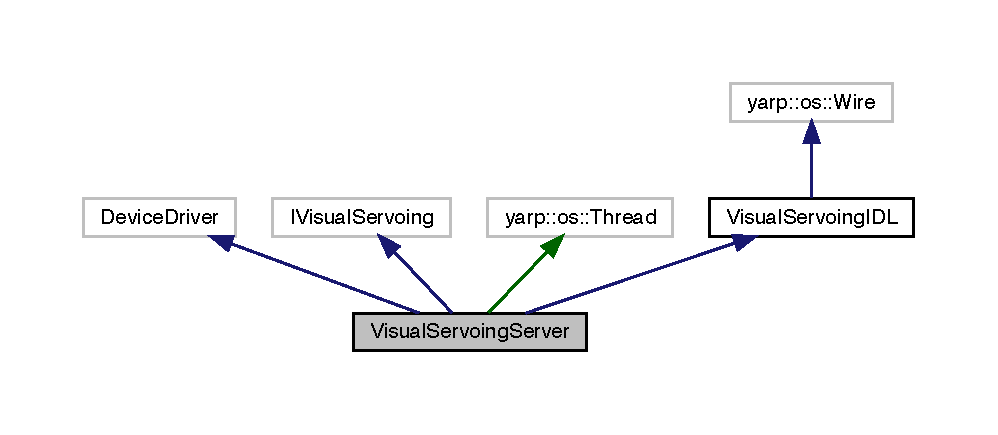
\includegraphics[width=350pt]{classVisualServoingServer__inherit__graph}
\end{center}
\end{figure}
\subsection*{Public Member Functions}
\begin{DoxyCompactItemize}
\item 
\hyperlink{classVisualServoingServer_a35df4de4c8cdb167b3eb15403beae653}{Visual\+Servoing\+Server} ()
\item 
\hyperlink{classVisualServoingServer_abb0f23eae68c9f453a5d66051744cadf}{$\sim$\+Visual\+Servoing\+Server} ()
\item 
bool \hyperlink{classVisualServoingServer_a0698977ddac02801eba3c35b47b9aa19}{open} (yarp\+::os\+::\+Searchable \&config) override
\item 
bool \hyperlink{classVisualServoingServer_ad9679d0bc524de74f4e96a1e8be23ca0}{close} () override
\item 
bool \hyperlink{classVisualServoingServer_a136cfac8840eda92c012851149b8624a}{init\+Facilities} (const bool use\+\_\+direct\+\_\+kin) override
\item 
bool \hyperlink{classVisualServoingServer_a39ea1de5ec159bd6779929c2bff84450}{reset\+Facilities} () override
\item 
bool \hyperlink{classVisualServoingServer_a0cd7a77750df9c1faaf1a18be6305de9}{stop\+Facilities} () override
\item 
bool \hyperlink{classVisualServoingServer_a085bb298e50f295d670bff6e4cb808d8}{go\+To\+Goal} (const yarp\+::sig\+::\+Vector \&vec\+\_\+x, const yarp\+::sig\+::\+Vector \&vec\+\_\+o) override
\item 
bool \hyperlink{classVisualServoingServer_a40ab9e9804793a58243077f31a2d79a4}{go\+To\+Goal} (const std\+::vector$<$ yarp\+::sig\+::\+Vector $>$ \&vec\+\_\+px\+\_\+l, const std\+::vector$<$ yarp\+::sig\+::\+Vector $>$ \&vec\+\_\+px\+\_\+r) override
\item 
bool \hyperlink{classVisualServoingServer_a6adf93e234e936879efe30cb9788b7ad}{set\+Modality} (const std\+::string \&mode) override
\item 
bool \hyperlink{classVisualServoingServer_a4a3ab24e71fed8052b04a9775cc86764}{set\+Visual\+Servo\+Control} (const std\+::string \&control) override
\item 
bool \hyperlink{classVisualServoingServer_a437c76c0ac9751cab05c76cd1f571d9b}{set\+Control\+Point} (const yarp\+::os\+::\+Const\+String \&point) override
\item 
bool \hyperlink{classVisualServoingServer_a66db1dfa1ebde34ada94bc36248e2ec8}{get\+Visual\+Servoing\+Info} (yarp\+::os\+::\+Bottle \&info) override
\item 
bool \hyperlink{classVisualServoingServer_ad632db85663df2f8c7ca5c27eaacfd71}{set\+Go\+To\+Goal\+Tolerance} (const double tol=15.\+0) override
\item 
bool \hyperlink{classVisualServoingServer_afa417f05dd02d2e91ff2c848f082a33b}{check\+Visual\+Servoing\+Controller} () override
\item 
bool \hyperlink{classVisualServoingServer_a3b462062db0cdcf3c8777469376bb5b6}{wait\+Visual\+Servoing\+Done} (const double period=0.\+1, const double timeout=0.\+0) override
\item 
bool \hyperlink{classVisualServoingServer_a4a21e5698a1d3b8db7c82772252bd215}{stop\+Controller} () override
\item 
bool \hyperlink{classVisualServoingServer_ab995d07572eb6e1103c73cc190c00e4a}{set\+Translation\+Gain} (const double K\+\_\+x\+\_\+1=1.\+0, const double K\+\_\+x\+\_\+2=0.\+25) override
\item 
bool \hyperlink{classVisualServoingServer_aa9b4b1b69b8600d7eac62a66af483bdb}{set\+Max\+Translation\+Velocity} (const double max\+\_\+x\+\_\+dot) override
\item 
bool \hyperlink{classVisualServoingServer_a5274182a8ff476c6b734ddf7cc78bef2}{set\+Translation\+Gain\+Switch\+Tolerance} (const double K\+\_\+x\+\_\+tol=30.\+0) override
\item 
bool \hyperlink{classVisualServoingServer_afb7ac6f85a55f928aa75134ba0ad1d79}{set\+Orientation\+Gain} (const double K\+\_\+x\+\_\+1=1.\+5, const double K\+\_\+x\+\_\+2=0.\+375) override
\item 
bool \hyperlink{classVisualServoingServer_a9f93de2ddb7818555bebad9ad0705029}{set\+Max\+Orientation\+Velocity} (const double max\+\_\+o\+\_\+dot) override
\item 
bool \hyperlink{classVisualServoingServer_a5a32f1ee99bff8b8a34d3825c30ffffc}{set\+Orientation\+Gain\+Switch\+Tolerance} (const double K\+\_\+o\+\_\+tol=30.\+0) override
\item 
std\+::vector$<$ yarp\+::sig\+::\+Vector $>$ \hyperlink{classVisualServoingServer_acc8932e08714c503ba6cfda11461976e}{get3\+D\+Goal\+Positions\+From3\+D\+Pose} (const yarp\+::sig\+::\+Vector \&x, const yarp\+::sig\+::\+Vector \&o) override
\item 
std\+::vector$<$ yarp\+::sig\+::\+Vector $>$ \hyperlink{classVisualServoingServer_a9d35a09c55cc8c059dc7bdbeeed8cfb1}{get\+Goal\+Pixels\+From3\+D\+Pose} (const yarp\+::sig\+::\+Vector \&x, const yarp\+::sig\+::\+Vector \&o, const Cam\+Sel \&cam) override
\item 
bool \hyperlink{classVisualServoingServer_abf97ec3877e208f4e889a094298a1e1a}{stored\+Init} (const std\+::string \&label) override
\item 
bool \hyperlink{classVisualServoingServer_a6d6ec7fee5b76d8a59d75a626b1bd11b}{stored\+Go\+To\+Goal} (const std\+::string \&label) override
\item 
bool \hyperlink{classVisualServoingServer_a6d051da5da8c07b0e0879d5af50a248f}{go\+To\+S\+F\+M\+Goal} () override
\item 
virtual bool \hyperlink{classVisualServoingIDL_a75929f915651161c43ed032e9f69a361}{go\+\_\+to\+\_\+px\+\_\+goal} (const std\+::vector$<$ std\+::vector$<$ double $>$ $>$ \&vec\+\_\+px\+\_\+l, const std\+::vector$<$ std\+::vector$<$ double $>$ $>$ \&vec\+\_\+px\+\_\+r)
\begin{DoxyCompactList}\small\item\em Set the goal points on both left and right camera image plane and start visual servoing. \end{DoxyCompactList}\item 
virtual bool \hyperlink{classVisualServoingIDL_a97106bf829447896de03680d78b960a5}{read} (yarp\+::os\+::\+Connection\+Reader \&connection) override
\item 
virtual std\+::vector$<$ std\+::string $>$ \hyperlink{classVisualServoingIDL_a99974ef8858179f14e2762c2d7bf4ed5}{help} (const std\+::string \&function\+Name=\char`\"{}-\/-\/all\char`\"{})
\end{DoxyCompactItemize}
\subsection*{Protected Types}
\begin{DoxyCompactItemize}
\item 
enum \hyperlink{classVisualServoingServer_ad7f000a91f0fc3423b86f2d2a584c4d3}{Visual\+Servo\+Control} \{ \hyperlink{classVisualServoingServer_ad7f000a91f0fc3423b86f2d2a584c4d3a8c5f04f9df63b44bea9b7edcb4dd1038}{Visual\+Servo\+Control\+::decoupled}, 
\hyperlink{classVisualServoingServer_ad7f000a91f0fc3423b86f2d2a584c4d3a00bd624b5b21d2b07edf398c1ce98b5e}{Visual\+Servo\+Control\+::robust}, 
\hyperlink{classVisualServoingServer_ad7f000a91f0fc3423b86f2d2a584c4d3a7949e6c02de2124dcdddd71b5430b8f0}{Visual\+Servo\+Control\+::cartesian}
 \}
\item 
enum \hyperlink{classVisualServoingServer_a3a1cce02f57cebb9056da5653d4dff0e}{Pixel\+Control\+Mode} \{ \hyperlink{classVisualServoingServer_a3a1cce02f57cebb9056da5653d4dff0eaa181a603769c1f98ad927e7367c7aa51}{Pixel\+Control\+Mode\+::all}, 
\hyperlink{classVisualServoingServer_a3a1cce02f57cebb9056da5653d4dff0ea9dd4e461268c8034f5c8564e155c67a6}{Pixel\+Control\+Mode\+::x}, 
\hyperlink{classVisualServoingServer_a3a1cce02f57cebb9056da5653d4dff0ead95679752134a2d9eb61dbd7b91c4bcc}{Pixel\+Control\+Mode\+::o}
 \}
\item 
enum \hyperlink{classVisualServoingServer_ab4ac95327e1829713374ca3cd0dec915}{Operating\+Mode} \{ \hyperlink{classVisualServoingServer_ab4ac95327e1829713374ca3cd0dec915a4757fe07fd492a8be0ea6a760d683d6e}{Operating\+Mode\+::position}, 
\hyperlink{classVisualServoingServer_ab4ac95327e1829713374ca3cd0dec915ada1639422ad8f355d2371428471379b5}{Operating\+Mode\+::orientation}, 
\hyperlink{classVisualServoingServer_ab4ac95327e1829713374ca3cd0dec915a2d5f8ae9328c6535be72ed28bff47560}{Operating\+Mode\+::pose}
 \}
\end{DoxyCompactItemize}
\subsection*{Protected Member Functions}
\begin{DoxyCompactItemize}
\item 
void \hyperlink{classVisualServoingServer_a4f23c649522804e21c7e60655a5dad99}{before\+Start} () override
\item 
bool \hyperlink{classVisualServoingServer_aa8673d3ac18d4aa4be94e8354ef0bad5}{thread\+Init} () override
\item 
void \hyperlink{classVisualServoingServer_a2397c1d1c5a5c65d1851075947f61f7e}{run} () override
\item 
void \hyperlink{classVisualServoingServer_ae6977911d131001eb4c9a07b83495518}{after\+Start} (bool success) override
\item 
void \hyperlink{classVisualServoingServer_a1401f7ee34d88728dd103439b25f9cf5}{on\+Stop} () override
\item 
void \hyperlink{classVisualServoingServer_a65744a18718c014e19f882dc1052a517}{thread\+Release} () override
\item 
bool \hyperlink{classVisualServoingServer_ad3668e0fc8818f9d2827bbc50087d353}{init\+\_\+facilities} (const bool use\+\_\+direct\+\_\+kin) override
\begin{DoxyCompactList}\small\item\em Initialize support modules and connections to perform a visual servoing task. \end{DoxyCompactList}\item 
bool \hyperlink{classVisualServoingServer_ae397fa9823f425fccf2837122629383f}{reset\+\_\+facilities} () override
\begin{DoxyCompactList}\small\item\em Reset support modules and connections to perform the current initialized visual servoing task. \end{DoxyCompactList}\item 
bool \hyperlink{classVisualServoingServer_ae5e4ac8d334374f2de259a530781443b}{stop\+\_\+facilities} () override
\begin{DoxyCompactList}\small\item\em Stop and disconnect support modules and connections used for visual servoing. \end{DoxyCompactList}\item 
bool \hyperlink{classVisualServoingServer_a6b68da9fe211a5779fc7a24e406dc8f0}{go\+\_\+to\+\_\+px\+\_\+goal} (const std\+::vector$<$ std\+::vector$<$ double $>$$>$ \&vec\+\_\+px\+\_\+l, const std\+::vector$<$ std\+::vector$<$ double $>$$>$ \&vec\+\_\+px\+\_\+r) override
\item 
bool \hyperlink{classVisualServoingServer_a77f26ac40c67d7a9b7e4ad7840532681}{go\+\_\+to\+\_\+pose\+\_\+goal} (const std\+::vector$<$ double $>$ \&vec\+\_\+x, const std\+::vector$<$ double $>$ \&vec\+\_\+o) override
\begin{DoxyCompactList}\small\item\em Set the goal point (3D for the position + 4D axis-\/angle for the orientation) and start visual servoing. \end{DoxyCompactList}\item 
bool \hyperlink{classVisualServoingServer_a6d9ec4489caebf0a52b2e5ee149aeb6d}{set\+\_\+modality} (const std\+::string \&mode) override
\begin{DoxyCompactList}\small\item\em Set visual servoing operating mode between\+: \end{DoxyCompactList}\item 
bool \hyperlink{classVisualServoingServer_a2f28e67b1dd44d9afba4a79fd89f4bc8}{set\+\_\+visual\+\_\+servo\+\_\+control} (const std\+::string \&control) override
\begin{DoxyCompactList}\small\item\em Set visual servo control law between\+: \end{DoxyCompactList}\item 
bool \hyperlink{classVisualServoingServer_a4a20a08fec9cfa4765e1245cfce5f9a8}{set\+\_\+control\+\_\+point} (const std\+::string \&point) override
\begin{DoxyCompactList}\small\item\em Set the point controlled during visual servoing. \end{DoxyCompactList}\item 
std\+::vector$<$ std\+::string $>$ \hyperlink{classVisualServoingServer_af085e2c5d4c4cfe940b3564b4ba69af6}{get\+\_\+visual\+\_\+servoing\+\_\+info} () override
\begin{DoxyCompactList}\small\item\em Return useful information for visual servoing. \end{DoxyCompactList}\item 
bool \hyperlink{classVisualServoingServer_a0efdb8edb2e4b91dc3168b5051b27f56}{set\+\_\+go\+\_\+to\+\_\+goal\+\_\+tolerance} (const double tol) override
\begin{DoxyCompactList}\small\item\em Set visual servoing goal tolerance. \end{DoxyCompactList}\item 
bool \hyperlink{classVisualServoingServer_a17a9b2913815c52b5a1bd2fd84d9f18e}{check\+\_\+visual\+\_\+servoing\+\_\+controller} () override
\begin{DoxyCompactList}\small\item\em Check once whether the visual servoing controller is running or not. \end{DoxyCompactList}\item 
bool \hyperlink{classVisualServoingServer_afcd501bb1d5070e8a0735f422a4c9ac0}{wait\+\_\+visual\+\_\+servoing\+\_\+done} (const double period, const double timeout) override
\begin{DoxyCompactList}\small\item\em Wait until visual servoing reaches the goal. \end{DoxyCompactList}\item 
bool \hyperlink{classVisualServoingServer_ac8d5b33c4ae61707e121c5154a973ab8}{stop\+\_\+controller} () override
\begin{DoxyCompactList}\small\item\em Ask for an immediate stop of the visual servoing controller. \end{DoxyCompactList}\item 
bool \hyperlink{classVisualServoingServer_a66324b38d90efb1e68cdfff9fd969487}{set\+\_\+translation\+\_\+gain} (const double K\+\_\+x\+\_\+1, const double K\+\_\+x\+\_\+2) override
\begin{DoxyCompactList}\small\item\em Set the translation gains of the visual servoing control algorithm. \end{DoxyCompactList}\item 
bool \hyperlink{classVisualServoingServer_a393d1a1d1a7a68fc2098a7c7e8724cc9}{set\+\_\+max\+\_\+translation\+\_\+velocity} (const double max\+\_\+x\+\_\+dot) override
\begin{DoxyCompactList}\small\item\em Set the maximum translation velocity of the visual servoing control algorithm (same for each axis). \end{DoxyCompactList}\item 
bool \hyperlink{classVisualServoingServer_a280690a55037cfaaacd39ca95470a507}{set\+\_\+translation\+\_\+gain\+\_\+switch\+\_\+tolerance} (const double K\+\_\+x\+\_\+tol) override
\begin{DoxyCompactList}\small\item\em Set the tolerance, in pixels, at which the translation control law swithces its gain value. \end{DoxyCompactList}\item 
bool \hyperlink{classVisualServoingServer_a19bdb0b44a8b556bad599dc03fca5f3f}{set\+\_\+orientation\+\_\+gain} (const double K\+\_\+o\+\_\+1, const double K\+\_\+o\+\_\+2) override
\begin{DoxyCompactList}\small\item\em Set the orientation gains of the visual servoing control algorithm. \end{DoxyCompactList}\item 
bool \hyperlink{classVisualServoingServer_aa3226ef2de2c1743e67788d1bff60679}{set\+\_\+max\+\_\+orientation\+\_\+velocity} (const double max\+\_\+o\+\_\+dot) override
\begin{DoxyCompactList}\small\item\em Set the maximum angular velocity of the axis-\/angle velocity vector of the visual servoing control algorithm. \end{DoxyCompactList}\item 
bool \hyperlink{classVisualServoingServer_a7d8c034f8a133f13ba9b4060ebcaf4bb}{set\+\_\+orientation\+\_\+gain\+\_\+switch\+\_\+tolerance} (const double K\+\_\+o\+\_\+tol) override
\begin{DoxyCompactList}\small\item\em Set the tolerance, in pixels, at which the orientation control law swithces its gain value. \end{DoxyCompactList}\item 
std\+::vector$<$ std\+::vector$<$ double $>$ $>$ \hyperlink{classVisualServoingServer_a542e0a6bf6158563a601740363911474}{get\+\_\+3\+D\+\_\+goal\+\_\+positions\+\_\+from\+\_\+3\+D\+\_\+pose} (const std\+::vector$<$ double $>$ \&x, const std\+::vector$<$ double $>$ \&o) override
\begin{DoxyCompactList}\small\item\em Helper function\+: extract four Cartesian points lying on the plane defined by the frame o in the position x relative to the robot base frame. \end{DoxyCompactList}\item 
std\+::vector$<$ std\+::vector$<$ double $>$ $>$ \hyperlink{classVisualServoingServer_aaa84d7964120ee1056f422dc2d5eb070}{get\+\_\+goal\+\_\+pixels\+\_\+from\+\_\+3\+D\+\_\+pose} (const std\+::vector$<$ double $>$ \&x, const std\+::vector$<$ double $>$ \&o, const std\+::string \&cam) override
\begin{DoxyCompactList}\small\item\em Helper function\+: extract four 2D pixel points lying on the plane defined by the frame o in the position x relative to the robot base frame. \end{DoxyCompactList}\item 
bool \hyperlink{classVisualServoingServer_ac438c7abfb838df458f85e250ead3222}{quit} () override
\begin{DoxyCompactList}\small\item\em Gently close the visual servoing device, deallocating resources. \end{DoxyCompactList}\item 
bool \hyperlink{classVisualServoingServer_aded37e0e0111c40fe5f869b16bb1f799}{stored\+\_\+init} (const std\+::string \&label) override
\begin{DoxyCompactList}\small\item\em Initialize the robot to an initial position. \end{DoxyCompactList}\item 
bool \hyperlink{classVisualServoingServer_a1c5018056e6a7db492cc6b1418f8d1e5}{stored\+\_\+go\+\_\+to\+\_\+goal} (const std\+::string \&label) override
\begin{DoxyCompactList}\small\item\em Set the robot visual servoing goal. \end{DoxyCompactList}\item 
bool \hyperlink{classVisualServoingServer_a3b0e5078c2f32493a2ef31ea32450d80}{get\+\_\+goal\+\_\+from\+\_\+sfm} () override
\begin{DoxyCompactList}\small\item\em Get goal point from S\+FM module. \end{DoxyCompactList}\end{DoxyCompactItemize}
\subsection*{Private Member Functions}
\begin{DoxyCompactItemize}
\item 
void \hyperlink{classVisualServoingServer_a79aafac31c32f2028836e1ef0f69dd99}{decoupled\+Image\+Based\+Visual\+Servo\+Control} ()
\item 
void \hyperlink{classVisualServoingServer_a34576cda7f4ed36dfae809a48f364d2b}{robust\+Image\+Based\+Visual\+Servo\+Control} ()
\item 
void \hyperlink{classVisualServoingServer_a9ad2bd94ff95fde9e309c4fb62de7377}{cartesian\+Position\+Based\+Visual\+Servo\+Control} ()
\item 
bool \hyperlink{classVisualServoingServer_a080585bc03f073b70a10bcdd6b36b309}{set\+Right\+Arm\+Cartesian\+Controller} ()
\item 
bool \hyperlink{classVisualServoingServer_a1cea1b6c32f9719cd63c36224fc1b9d2}{set\+Gaze\+Controller} ()
\item 
bool \hyperlink{classVisualServoingServer_a27c26de8415dee1c3165edd1e1d362a2}{set\+Command\+Port} ()
\item 
bool \hyperlink{classVisualServoingServer_a9e031793c83063b80035f8769d28a99f}{set\+Torso\+D\+OF} ()
\item 
bool \hyperlink{classVisualServoingServer_a509750822f0f1e0db26d54288f8eb1fd}{unset\+Torso\+D\+OF} ()
\item 
std\+::vector$<$ yarp\+::sig\+::\+Vector $>$ \hyperlink{classVisualServoingServer_a04f3caed0ac350b3579efeb4cd548eb8}{get\+Pixels\+From\+Pose} (const yarp\+::sig\+::\+Vector \&pose, const Cam\+Sel \&cam)
\item 
std\+::vector$<$ yarp\+::sig\+::\+Vector $>$ \hyperlink{classVisualServoingServer_a67bfc714271a28bf55fa49c89019b53c}{get\+Control\+Pixels\+From\+Pose} (const yarp\+::sig\+::\+Vector \&pose, const Cam\+Sel \&cam, const \hyperlink{classVisualServoingServer_a3a1cce02f57cebb9056da5653d4dff0e}{Pixel\+Control\+Mode} \&mode)
\item 
std\+::vector$<$ yarp\+::sig\+::\+Vector $>$ \hyperlink{classVisualServoingServer_ac9e6020f30b6df05db3fc34a44fee0d4}{get\+Control\+Points\+From\+Pose} (const yarp\+::sig\+::\+Vector \&pose)
\item 
yarp\+::sig\+::\+Vector \hyperlink{classVisualServoingServer_a997029621c723c1e9962b35a917167cc}{get\+Pixel\+From\+Point} (const Cam\+Sel \&cam, const yarp\+::sig\+::\+Vector \&p) const
\item 
yarp\+::sig\+::\+Vector \hyperlink{classVisualServoingServer_a43cf45e933a71214cfb4d8248005761e}{get\+Control\+Pixel\+From\+Point} (const Cam\+Sel \&cam, const yarp\+::sig\+::\+Vector \&p) const
\item 
void \hyperlink{classVisualServoingServer_ad5334ed717f373cfbd40290824d9ed1f}{get\+Current\+Stereo\+Features\+And\+Jacobian} (const std\+::vector$<$ yarp\+::sig\+::\+Vector $>$ \&left\+\_\+px, const std\+::vector$<$ yarp\+::sig\+::\+Vector $>$ \&right\+\_\+px, yarp\+::sig\+::\+Vector \&features, yarp\+::sig\+::\+Matrix \&jacobian)
\item 
yarp\+::sig\+::\+Vector \hyperlink{classVisualServoingServer_a3aa225c2c4f417c4ea7dd27e9b6d0c8a}{get\+JacobianU} (const Cam\+Sel \&cam, const yarp\+::sig\+::\+Vector \&px)
\item 
yarp\+::sig\+::\+Vector \hyperlink{classVisualServoingServer_a51667642f6d882df082f79ec01111181}{get\+JacobianV} (const Cam\+Sel \&cam, const yarp\+::sig\+::\+Vector \&px)
\item 
bool \hyperlink{classVisualServoingServer_a141036fb33bfb74199691ad444b29082}{set\+Camera\+Transformations} ()
\item 
bool \hyperlink{classVisualServoingServer_a53616791e66a24c1131e2cb3a3634a6d}{set\+Pose\+Goal} (const yarp\+::sig\+::\+Vector \&goal\+\_\+x, const yarp\+::sig\+::\+Vector \&goal\+\_\+o)
\item 
bool \hyperlink{classVisualServoingServer_aea96fc77c6255e0826bd17190214a29b}{set\+Pixel\+Goal} (const std\+::vector$<$ yarp\+::sig\+::\+Vector $>$ \&l\+\_\+px\+\_\+goal, const std\+::vector$<$ yarp\+::sig\+::\+Vector $>$ \&r\+\_\+px\+\_\+goal)
\item 
void \hyperlink{classVisualServoingServer_abe1d3c25e81378f9a1a834d64cf0c496}{backproc\+\_\+\+Update\+Visual\+Servoing\+Paramters} ()
\item 
yarp\+::sig\+::\+Vector \hyperlink{classVisualServoingServer_a66e3aaa742d5b0d23a6d3a33a800c088}{average\+Pose} (const yarp\+::sig\+::\+Vector \&l\+\_\+pose, const yarp\+::sig\+::\+Vector \&r\+\_\+pose) const
\item 
bool \hyperlink{classVisualServoingServer_a6201a672d3efe497dd0114df50aee4d7}{check\+Visual\+Servoing\+Status} (const yarp\+::sig\+::\+Vector \&px\+\_\+cur, const double tol)
\item 
bool \hyperlink{classVisualServoingServer_afbcab623f48e3d2e648e144e22df4f19}{check\+Visual\+Servoing\+Status} (const yarp\+::sig\+::\+Vector \&pose\+\_\+cur, const double tol\+\_\+position, const double tol\+\_\+orientation, const double tol\+\_\+angle)
\item 
void \hyperlink{classVisualServoingServer_a6b16f76335ebbd9e4ba9e5ddb67cf883}{y\+Info\+Verbose} (const yarp\+::os\+::\+Const\+String \&str) const
\item 
void \hyperlink{classVisualServoingServer_a570985820c386689a9507066a016b839}{y\+Warning\+Verbose} (const yarp\+::os\+::\+Const\+String \&str) const
\item 
void \hyperlink{classVisualServoingServer_a8eb3cf6c73a515f6f435f01327d37bd1}{y\+Error\+Verbose} (const yarp\+::os\+::\+Const\+String \&str) const
\item 
yarp\+::sig\+::\+Vector \hyperlink{classVisualServoingServer_adcc6db0a6cf857c4bd44d495ec445954}{std\+Vector\+Of\+Vectors\+To\+Vector} (const std\+::vector$<$ yarp\+::sig\+::\+Vector $>$ \&vectors)
\end{DoxyCompactItemize}
\subsection*{Private Attributes}
\begin{DoxyCompactItemize}
\item 
bool \hyperlink{classVisualServoingServer_a559b6106818be3b9c48352b614e658c7}{verbosity\+\_\+} = false
\item 
bool \hyperlink{classVisualServoingServer_ad847ce0f5480013481f037bc554ae96e}{sim\+\_\+} = false
\item 
yarp\+::os\+::\+Const\+String \hyperlink{classVisualServoingServer_adb8cccbe6de08ec4b686d2eca8a99dfd}{robot\+\_\+name\+\_\+} = \char`\"{}icub\char`\"{}
\item 
\hyperlink{classVisualServoingServer_ad7f000a91f0fc3423b86f2d2a584c4d3}{Visual\+Servo\+Control} \hyperlink{classVisualServoingServer_ac8da8eea9620e8cce4ba2502bb1ec86a}{vs\+\_\+control\+\_\+} = \hyperlink{classVisualServoingServer_ad7f000a91f0fc3423b86f2d2a584c4d3a8c5f04f9df63b44bea9b7edcb4dd1038}{Visual\+Servo\+Control\+::decoupled}
\item 
\hyperlink{classVisualServoingServer_ab4ac95327e1829713374ca3cd0dec915}{Operating\+Mode} \hyperlink{classVisualServoingServer_af6b808cf1ef56df5fb432196335e1ceb}{op\+\_\+mode\+\_\+} = \hyperlink{classVisualServoingServer_ab4ac95327e1829713374ca3cd0dec915a2d5f8ae9328c6535be72ed28bff47560}{Operating\+Mode\+::pose}
\item 
yarp\+::dev\+::\+Poly\+Driver \hyperlink{classVisualServoingServer_a46e47b0abc5b52fbba314cf9c2ce0df5}{rightarm\+\_\+cartesian\+\_\+driver\+\_\+}
\item 
yarp\+::dev\+::\+I\+Cartesian\+Control $\ast$ \hyperlink{classVisualServoingServer_a62c8f5c6ba2d62db4754d94984b98632}{itf\+\_\+rightarm\+\_\+cart\+\_\+}
\item 
yarp\+::dev\+::\+Poly\+Driver \hyperlink{classVisualServoingServer_a5da42a79826f631e1e40b723e3620c0a}{gaze\+\_\+driver\+\_\+}
\item 
yarp\+::dev\+::\+I\+Gaze\+Control $\ast$ \hyperlink{classVisualServoingServer_ac884095733af31af336373edbe09eae3}{itf\+\_\+gaze\+\_\+}
\item 
bool \hyperlink{classVisualServoingServer_aeb48fa3b045d9fb074b03ea9d8441972}{vs\+\_\+control\+\_\+running\+\_\+} = false
\item 
bool \hyperlink{classVisualServoingServer_aae9c2aa802fa83d8b77b5094af94fa38}{vs\+\_\+goal\+\_\+reached\+\_\+} = false
\item 
const double \hyperlink{classVisualServoingServer_a48bcc91d15c80f7b3b248fa205e8e3de}{Ts\+\_\+} = 0.\+1
\item 
std\+::array$<$ double, 2 $>$ \hyperlink{classVisualServoingServer_a6153b1e315817cf41cb36b7deca83be7}{K\+\_\+x\+\_\+} = \{\{0.\+5, 0.\+25\}\}
\item 
std\+::array$<$ double, 2 $>$ \hyperlink{classVisualServoingServer_a5a7eaa18a77566e129a325e556691e24}{K\+\_\+o\+\_\+} = \{\{3.\+5, 0.\+5\}\}
\item 
double \hyperlink{classVisualServoingServer_a82df6acf27455af727ce31758856ee48}{max\+\_\+x\+\_\+dot\+\_\+} = 0.\+035
\item 
double \hyperlink{classVisualServoingServer_a2fb091edd86b425b79b36c968a0929e1}{max\+\_\+o\+\_\+dot\+\_\+} = 10.\+0 $\ast$ M\+\_\+\+PI / 180.\+0
\item 
double \hyperlink{classVisualServoingServer_aa59bfed390207a42a4a05dd1fe720f6b}{K\+\_\+x\+\_\+tol\+\_\+} = 10.\+0
\item 
double \hyperlink{classVisualServoingServer_ab372aee55fa6ffb7d87d0f9103ea3266}{K\+\_\+o\+\_\+tol\+\_\+} = 10.\+0
\item 
double \hyperlink{classVisualServoingServer_aaef2ff3c3853c7a73bc620225f824e4e}{K\+\_\+position\+\_\+tol\+\_\+} = 0.\+03
\item 
double \hyperlink{classVisualServoingServer_ab1c7e6dbab2608694d520e849da043f8}{K\+\_\+orientation\+\_\+tol\+\_\+} = 9.\+0 $\ast$ M\+\_\+\+PI / 180.\+0
\item 
double \hyperlink{classVisualServoingServer_a3eaf0fc5ef519ebb94fc89f3a1e490a2}{K\+\_\+angle\+\_\+tol\+\_\+} = 3.\+0 $\ast$ M\+\_\+\+PI / 180.\+0
\item 
bool \hyperlink{classVisualServoingServer_a8b8f0cda1bb882c1783db88b720b5597}{K\+\_\+x\+\_\+hysteresis\+\_\+} = false
\item 
bool \hyperlink{classVisualServoingServer_a19e92e42912ae3f4d784d80465ed55b1}{K\+\_\+o\+\_\+hysteresis\+\_\+} = false
\item 
bool \hyperlink{classVisualServoingServer_a4fdd46d1c8be0e8eb8b28af84cfe8a6b}{K\+\_\+pose\+\_\+hysteresis\+\_\+} = false
\item 
double \hyperlink{classVisualServoingServer_a74ac88af1fee404c750afb59fad98fc6}{tol\+\_\+px\+\_\+} = 1.\+0
\item 
double \hyperlink{classVisualServoingServer_ab2cc91975c9a3f949a99fd6737a2b3bd}{tol\+\_\+position\+\_\+} = 0.\+01
\item 
double \hyperlink{classVisualServoingServer_a2ebbd8cf0f5bf0968bb574fbadb681e8}{tol\+\_\+orientation\+\_\+} = 3.\+0 $\ast$ M\+\_\+\+PI / 180.\+0
\item 
double \hyperlink{classVisualServoingServer_a8a39a62f89dc07cbfbdc91441ad71975}{tol\+\_\+angle\+\_\+} = 1.\+0 $\ast$ M\+\_\+\+PI / 180.\+0
\item 
double \hyperlink{classVisualServoingServer_ac397cdbba97a35d454ab2974db0c5005}{traj\+\_\+time\+\_\+} = 1.\+0
\item 
yarp\+::sig\+::\+Matrix \hyperlink{classVisualServoingServer_a19525066e8d98f781f28600ff526ce68}{l\+\_\+proj\+\_\+}
\item 
yarp\+::sig\+::\+Matrix \hyperlink{classVisualServoingServer_a5bd4d326f2247a39065747e937246677}{r\+\_\+proj\+\_\+}
\item 
yarp\+::sig\+::\+Vector \hyperlink{classVisualServoingServer_aadfea10f7ca8a2e745c4091d2a1b7c46}{goal\+\_\+pose\+\_\+} = yarp\+::math\+::zeros(7)
\item 
yarp\+::sig\+::\+Vector \hyperlink{classVisualServoingServer_a26d45260d6b8e1e17c57bf339890c124}{px\+\_\+des\+\_\+} = yarp\+::math\+::zeros(16)
\item 
yarp\+::sig\+::\+Matrix \hyperlink{classVisualServoingServer_afbf7be0f4c935dcbcd8a23b07b7972ba}{l\+\_\+\+H\+\_\+eye\+\_\+to\+\_\+r\+\_\+} = yarp\+::math\+::zeros(4, 4)
\item 
yarp\+::sig\+::\+Matrix \hyperlink{classVisualServoingServer_a5de06681532722dae98703c4d3e60ba1}{r\+\_\+\+H\+\_\+eye\+\_\+to\+\_\+r\+\_\+} = yarp\+::math\+::zeros(4, 4)
\item 
yarp\+::sig\+::\+Matrix \hyperlink{classVisualServoingServer_a43b53260b0903efb5479becf664f33ae}{l\+\_\+\+H\+\_\+r\+\_\+to\+\_\+cam\+\_\+} = yarp\+::math\+::zeros(4, 4)
\item 
yarp\+::sig\+::\+Matrix \hyperlink{classVisualServoingServer_a82bdf1e87c5f65bbbea97655a78fceb6}{r\+\_\+\+H\+\_\+r\+\_\+to\+\_\+cam\+\_\+} = yarp\+::math\+::zeros(4, 4)
\item 
std\+::mutex \hyperlink{classVisualServoingServer_a63758b38bb0069515d047449aafc9597}{mtx\+\_\+px\+\_\+des\+\_\+}
\item 
std\+::mutex \hyperlink{classVisualServoingServer_a379f8205d854495f481bbaa37825dfcb}{mtx\+\_\+\+H\+\_\+eye\+\_\+cam\+\_\+}
\item 
std\+::thread $\ast$ \hyperlink{classVisualServoingServer_a01078c56ef8966f186d5cbf22c8c1c0c}{thr\+\_\+background\+\_\+update\+\_\+params\+\_\+}
\item 
std\+::vector$<$ yarp\+::sig\+::\+Vector $>$ \hyperlink{classVisualServoingServer_a3f7efc9e5a4bbb030a4dd81030643398}{l\+\_\+px\+\_\+goal\+\_\+} = std\+::vector$<$yarp\+::sig\+::\+Vector$>$(4)
\item 
std\+::vector$<$ yarp\+::sig\+::\+Vector $>$ \hyperlink{classVisualServoingServer_a831ffb606b1ff70d0475b645441f469d}{r\+\_\+px\+\_\+goal\+\_\+} = std\+::vector$<$yarp\+::sig\+::\+Vector$>$(4)
\item 
int \hyperlink{classVisualServoingServer_a85d6a488bf20eaeb155677a80f731614}{ctx\+\_\+local\+\_\+cart\+\_\+}
\item 
int \hyperlink{classVisualServoingServer_a815f9069588f590419cd8645afd3f017}{ctx\+\_\+remote\+\_\+cart\+\_\+}
\item 
yarp\+::os\+::\+Buffered\+Port$<$ yarp\+::sig\+::\+Vector $>$ \hyperlink{classVisualServoingServer_a4c250786d095b0e8a8f5546b2976a669}{port\+\_\+pose\+\_\+left\+\_\+in\+\_\+}
\item 
yarp\+::os\+::\+Buffered\+Port$<$ yarp\+::sig\+::\+Vector $>$ \hyperlink{classVisualServoingServer_a708ab93d60ae60ae28fbe7a9f1bffe29}{port\+\_\+pose\+\_\+right\+\_\+in\+\_\+}
\item 
yarp\+::os\+::\+Buffered\+Port$<$ yarp\+::sig\+::\+Image\+Of$<$ yarp\+::sig\+::\+Pixel\+Rgb $>$ $>$ \hyperlink{classVisualServoingServer_a0561904e7a2d8f680812f042eec3b2d8}{port\+\_\+image\+\_\+left\+\_\+in\+\_\+}
\item 
yarp\+::os\+::\+Buffered\+Port$<$ yarp\+::sig\+::\+Image\+Of$<$ yarp\+::sig\+::\+Pixel\+Rgb $>$ $>$ \hyperlink{classVisualServoingServer_ac8e9e8c8e3c0a412bd1dd464b58931bd}{port\+\_\+image\+\_\+left\+\_\+out\+\_\+}
\item 
yarp\+::os\+::\+Buffered\+Port$<$ yarp\+::os\+::\+Bottle $>$ \hyperlink{classVisualServoingServer_a46d59d98a68e0a88b810835c447241f6}{port\+\_\+click\+\_\+left\+\_\+}
\item 
yarp\+::os\+::\+Buffered\+Port$<$ yarp\+::sig\+::\+Image\+Of$<$ yarp\+::sig\+::\+Pixel\+Rgb $>$ $>$ \hyperlink{classVisualServoingServer_a776855ca4deb47cf1c739bde2e07bc8e}{port\+\_\+image\+\_\+right\+\_\+in\+\_\+}
\item 
yarp\+::os\+::\+Buffered\+Port$<$ yarp\+::sig\+::\+Image\+Of$<$ yarp\+::sig\+::\+Pixel\+Rgb $>$ $>$ \hyperlink{classVisualServoingServer_ab5c7a20d3e8545331970517c75d79f2a}{port\+\_\+image\+\_\+right\+\_\+out\+\_\+}
\item 
yarp\+::os\+::\+Buffered\+Port$<$ yarp\+::os\+::\+Bottle $>$ \hyperlink{classVisualServoingServer_a67701a55fce8ed1301417ecda99eff06}{port\+\_\+click\+\_\+right\+\_\+}
\item 
yarp\+::os\+::\+Port \hyperlink{classVisualServoingServer_af10ae1004d335193ab8bd23821a6007f}{port\+\_\+rpc\+\_\+command\+\_\+}
\item 
yarp\+::os\+::\+Rpc\+Client \hyperlink{classVisualServoingServer_a3835afd8ec4c21b2c1d217f7d68a71bb}{port\+\_\+rpc\+\_\+tracker\+\_\+left\+\_\+}
\item 
yarp\+::os\+::\+Rpc\+Client \hyperlink{classVisualServoingServer_a36df02520e7cc2814d8404e05a42409b}{port\+\_\+rpc\+\_\+tracker\+\_\+right\+\_\+}
\item 
bool \hyperlink{classVisualServoingServer_a36243aeb865e36c5e91d3cd3375b9f29}{is\+\_\+stopping\+\_\+backproc\+\_\+update\+\_\+vs\+\_\+params} = true
\item 
yarp\+::os\+::\+Buffered\+Port$<$ yarp\+::sig\+::\+Vector $>$ \hyperlink{classVisualServoingServer_aa72393af28f4b424eeb2966962cbd319}{port\+\_\+pose\+\_\+px\+\_\+l\+\_\+}
\item 
yarp\+::os\+::\+Buffered\+Port$<$ yarp\+::sig\+::\+Vector $>$ \hyperlink{classVisualServoingServer_ab068de8542a539175a18d698e5b2289f}{port\+\_\+pose\+\_\+px\+\_\+r\+\_\+}
\item 
yarp\+::os\+::\+Buffered\+Port$<$ yarp\+::sig\+::\+Vector $>$ \hyperlink{classVisualServoingServer_a5c6969762a136abeb5de050637e6fbc7}{port\+\_\+kin\+\_\+px\+\_\+l\+\_\+}
\item 
yarp\+::os\+::\+Buffered\+Port$<$ yarp\+::sig\+::\+Vector $>$ \hyperlink{classVisualServoingServer_a0a681791d720678229a3365a5bb0bfd6}{port\+\_\+kin\+\_\+px\+\_\+r\+\_\+}
\item 
yarp\+::os\+::\+Buffered\+Port$<$ yarp\+::sig\+::\+Vector $>$ \hyperlink{classVisualServoingServer_ac4fad3f3691ad57d8a1f693e573f75be}{port\+\_\+goal\+\_\+px\+\_\+l\+\_\+}
\item 
yarp\+::os\+::\+Buffered\+Port$<$ yarp\+::sig\+::\+Vector $>$ \hyperlink{classVisualServoingServer_ad06d05e912dbba4c1ded31ae6e0e3004}{port\+\_\+goal\+\_\+px\+\_\+r\+\_\+}
\item 
yarp\+::os\+::\+Buffered\+Port$<$ yarp\+::sig\+::\+Vector $>$ \hyperlink{classVisualServoingServer_a31db93e3ee0db64e8681d762428b85a9}{port\+\_\+pose\+\_\+avg\+\_\+}
\item 
yarp\+::os\+::\+Buffered\+Port$<$ yarp\+::sig\+::\+Vector $>$ \hyperlink{classVisualServoingServer_a0f4787672f7b6dea128d688aff2056fc}{port\+\_\+pose\+\_\+kin\+\_\+}
\item 
yarp\+::os\+::\+Buffered\+Port$<$ yarp\+::sig\+::\+Vector $>$ \hyperlink{classVisualServoingServer_a73e57c16019ed76e14e92a600f1e761b}{port\+\_\+pose\+\_\+goal\+\_\+}
\end{DoxyCompactItemize}


\subsection{Detailed Description}


Definition at line 32 of file Visual\+Servoing\+Server.\+h.



\subsection{Member Enumeration Documentation}
\mbox{\Hypertarget{classVisualServoingServer_ab4ac95327e1829713374ca3cd0dec915}\label{classVisualServoingServer_ab4ac95327e1829713374ca3cd0dec915}} 
\index{Visual\+Servoing\+Server@{Visual\+Servoing\+Server}!Operating\+Mode@{Operating\+Mode}}
\index{Operating\+Mode@{Operating\+Mode}!Visual\+Servoing\+Server@{Visual\+Servoing\+Server}}
\subsubsection{\texorpdfstring{Operating\+Mode}{OperatingMode}}
{\footnotesize\ttfamily enum \hyperlink{classVisualServoingServer_ab4ac95327e1829713374ca3cd0dec915}{Visual\+Servoing\+Server\+::\+Operating\+Mode}\hspace{0.3cm}{\ttfamily [strong]}, {\ttfamily [protected]}}

\begin{DoxyEnumFields}{Enumerator}
\raisebox{\heightof{T}}[0pt][0pt]{\index{position@{position}!Visual\+Servoing\+Server@{Visual\+Servoing\+Server}}\index{Visual\+Servoing\+Server@{Visual\+Servoing\+Server}!position@{position}}}\mbox{\Hypertarget{classVisualServoingServer_ab4ac95327e1829713374ca3cd0dec915a4757fe07fd492a8be0ea6a760d683d6e}\label{classVisualServoingServer_ab4ac95327e1829713374ca3cd0dec915a4757fe07fd492a8be0ea6a760d683d6e}} 
position&\\
\hline

\raisebox{\heightof{T}}[0pt][0pt]{\index{orientation@{orientation}!Visual\+Servoing\+Server@{Visual\+Servoing\+Server}}\index{Visual\+Servoing\+Server@{Visual\+Servoing\+Server}!orientation@{orientation}}}\mbox{\Hypertarget{classVisualServoingServer_ab4ac95327e1829713374ca3cd0dec915ada1639422ad8f355d2371428471379b5}\label{classVisualServoingServer_ab4ac95327e1829713374ca3cd0dec915ada1639422ad8f355d2371428471379b5}} 
orientation&\\
\hline

\raisebox{\heightof{T}}[0pt][0pt]{\index{pose@{pose}!Visual\+Servoing\+Server@{Visual\+Servoing\+Server}}\index{Visual\+Servoing\+Server@{Visual\+Servoing\+Server}!pose@{pose}}}\mbox{\Hypertarget{classVisualServoingServer_ab4ac95327e1829713374ca3cd0dec915a2d5f8ae9328c6535be72ed28bff47560}\label{classVisualServoingServer_ab4ac95327e1829713374ca3cd0dec915a2d5f8ae9328c6535be72ed28bff47560}} 
pose&\\
\hline

\end{DoxyEnumFields}


Definition at line 174 of file Visual\+Servoing\+Server.\+h.

\mbox{\Hypertarget{classVisualServoingServer_a3a1cce02f57cebb9056da5653d4dff0e}\label{classVisualServoingServer_a3a1cce02f57cebb9056da5653d4dff0e}} 
\index{Visual\+Servoing\+Server@{Visual\+Servoing\+Server}!Pixel\+Control\+Mode@{Pixel\+Control\+Mode}}
\index{Pixel\+Control\+Mode@{Pixel\+Control\+Mode}!Visual\+Servoing\+Server@{Visual\+Servoing\+Server}}
\subsubsection{\texorpdfstring{Pixel\+Control\+Mode}{PixelControlMode}}
{\footnotesize\ttfamily enum \hyperlink{classVisualServoingServer_a3a1cce02f57cebb9056da5653d4dff0e}{Visual\+Servoing\+Server\+::\+Pixel\+Control\+Mode}\hspace{0.3cm}{\ttfamily [strong]}, {\ttfamily [protected]}}

\begin{DoxyEnumFields}{Enumerator}
\raisebox{\heightof{T}}[0pt][0pt]{\index{all@{all}!Visual\+Servoing\+Server@{Visual\+Servoing\+Server}}\index{Visual\+Servoing\+Server@{Visual\+Servoing\+Server}!all@{all}}}\mbox{\Hypertarget{classVisualServoingServer_a3a1cce02f57cebb9056da5653d4dff0eaa181a603769c1f98ad927e7367c7aa51}\label{classVisualServoingServer_a3a1cce02f57cebb9056da5653d4dff0eaa181a603769c1f98ad927e7367c7aa51}} 
all&\\
\hline

\raisebox{\heightof{T}}[0pt][0pt]{\index{x@{x}!Visual\+Servoing\+Server@{Visual\+Servoing\+Server}}\index{Visual\+Servoing\+Server@{Visual\+Servoing\+Server}!x@{x}}}\mbox{\Hypertarget{classVisualServoingServer_a3a1cce02f57cebb9056da5653d4dff0ea9dd4e461268c8034f5c8564e155c67a6}\label{classVisualServoingServer_a3a1cce02f57cebb9056da5653d4dff0ea9dd4e461268c8034f5c8564e155c67a6}} 
x&\\
\hline

\raisebox{\heightof{T}}[0pt][0pt]{\index{o@{o}!Visual\+Servoing\+Server@{Visual\+Servoing\+Server}}\index{Visual\+Servoing\+Server@{Visual\+Servoing\+Server}!o@{o}}}\mbox{\Hypertarget{classVisualServoingServer_a3a1cce02f57cebb9056da5653d4dff0ead95679752134a2d9eb61dbd7b91c4bcc}\label{classVisualServoingServer_a3a1cce02f57cebb9056da5653d4dff0ead95679752134a2d9eb61dbd7b91c4bcc}} 
o&\\
\hline

\end{DoxyEnumFields}


Definition at line 172 of file Visual\+Servoing\+Server.\+h.

\mbox{\Hypertarget{classVisualServoingServer_ad7f000a91f0fc3423b86f2d2a584c4d3}\label{classVisualServoingServer_ad7f000a91f0fc3423b86f2d2a584c4d3}} 
\index{Visual\+Servoing\+Server@{Visual\+Servoing\+Server}!Visual\+Servo\+Control@{Visual\+Servo\+Control}}
\index{Visual\+Servo\+Control@{Visual\+Servo\+Control}!Visual\+Servoing\+Server@{Visual\+Servoing\+Server}}
\subsubsection{\texorpdfstring{Visual\+Servo\+Control}{VisualServoControl}}
{\footnotesize\ttfamily enum \hyperlink{classVisualServoingServer_ad7f000a91f0fc3423b86f2d2a584c4d3}{Visual\+Servoing\+Server\+::\+Visual\+Servo\+Control}\hspace{0.3cm}{\ttfamily [strong]}, {\ttfamily [protected]}}

\begin{DoxyEnumFields}{Enumerator}
\raisebox{\heightof{T}}[0pt][0pt]{\index{decoupled@{decoupled}!Visual\+Servoing\+Server@{Visual\+Servoing\+Server}}\index{Visual\+Servoing\+Server@{Visual\+Servoing\+Server}!decoupled@{decoupled}}}\mbox{\Hypertarget{classVisualServoingServer_ad7f000a91f0fc3423b86f2d2a584c4d3a8c5f04f9df63b44bea9b7edcb4dd1038}\label{classVisualServoingServer_ad7f000a91f0fc3423b86f2d2a584c4d3a8c5f04f9df63b44bea9b7edcb4dd1038}} 
decoupled&\\
\hline

\raisebox{\heightof{T}}[0pt][0pt]{\index{robust@{robust}!Visual\+Servoing\+Server@{Visual\+Servoing\+Server}}\index{Visual\+Servoing\+Server@{Visual\+Servoing\+Server}!robust@{robust}}}\mbox{\Hypertarget{classVisualServoingServer_ad7f000a91f0fc3423b86f2d2a584c4d3a00bd624b5b21d2b07edf398c1ce98b5e}\label{classVisualServoingServer_ad7f000a91f0fc3423b86f2d2a584c4d3a00bd624b5b21d2b07edf398c1ce98b5e}} 
robust&\\
\hline

\raisebox{\heightof{T}}[0pt][0pt]{\index{cartesian@{cartesian}!Visual\+Servoing\+Server@{Visual\+Servoing\+Server}}\index{Visual\+Servoing\+Server@{Visual\+Servoing\+Server}!cartesian@{cartesian}}}\mbox{\Hypertarget{classVisualServoingServer_ad7f000a91f0fc3423b86f2d2a584c4d3a7949e6c02de2124dcdddd71b5430b8f0}\label{classVisualServoingServer_ad7f000a91f0fc3423b86f2d2a584c4d3a7949e6c02de2124dcdddd71b5430b8f0}} 
cartesian&\\
\hline

\end{DoxyEnumFields}


Definition at line 170 of file Visual\+Servoing\+Server.\+h.



\subsection{Constructor \& Destructor Documentation}
\mbox{\Hypertarget{classVisualServoingServer_a35df4de4c8cdb167b3eb15403beae653}\label{classVisualServoingServer_a35df4de4c8cdb167b3eb15403beae653}} 
\index{Visual\+Servoing\+Server@{Visual\+Servoing\+Server}!Visual\+Servoing\+Server@{Visual\+Servoing\+Server}}
\index{Visual\+Servoing\+Server@{Visual\+Servoing\+Server}!Visual\+Servoing\+Server@{Visual\+Servoing\+Server}}
\subsubsection{\texorpdfstring{Visual\+Servoing\+Server()}{VisualServoingServer()}}
{\footnotesize\ttfamily Visual\+Servoing\+Server\+::\+Visual\+Servoing\+Server (\begin{DoxyParamCaption}{ }\end{DoxyParamCaption})}



Definition at line 20 of file Visual\+Servoing\+Server.\+cpp.

\mbox{\Hypertarget{classVisualServoingServer_abb0f23eae68c9f453a5d66051744cadf}\label{classVisualServoingServer_abb0f23eae68c9f453a5d66051744cadf}} 
\index{Visual\+Servoing\+Server@{Visual\+Servoing\+Server}!````~Visual\+Servoing\+Server@{$\sim$\+Visual\+Servoing\+Server}}
\index{````~Visual\+Servoing\+Server@{$\sim$\+Visual\+Servoing\+Server}!Visual\+Servoing\+Server@{Visual\+Servoing\+Server}}
\subsubsection{\texorpdfstring{$\sim$\+Visual\+Servoing\+Server()}{~VisualServoingServer()}}
{\footnotesize\ttfamily Visual\+Servoing\+Server\+::$\sim$\+Visual\+Servoing\+Server (\begin{DoxyParamCaption}{ }\end{DoxyParamCaption})}



Definition at line 27 of file Visual\+Servoing\+Server.\+cpp.



\subsection{Member Function Documentation}
\mbox{\Hypertarget{classVisualServoingServer_ae6977911d131001eb4c9a07b83495518}\label{classVisualServoingServer_ae6977911d131001eb4c9a07b83495518}} 
\index{Visual\+Servoing\+Server@{Visual\+Servoing\+Server}!after\+Start@{after\+Start}}
\index{after\+Start@{after\+Start}!Visual\+Servoing\+Server@{Visual\+Servoing\+Server}}
\subsubsection{\texorpdfstring{after\+Start()}{afterStart()}}
{\footnotesize\ttfamily void Visual\+Servoing\+Server\+::after\+Start (\begin{DoxyParamCaption}\item[{bool}]{success }\end{DoxyParamCaption})\hspace{0.3cm}{\ttfamily [override]}, {\ttfamily [protected]}}



Definition at line 1032 of file Visual\+Servoing\+Server.\+cpp.

\mbox{\Hypertarget{classVisualServoingServer_a66e3aaa742d5b0d23a6d3a33a800c088}\label{classVisualServoingServer_a66e3aaa742d5b0d23a6d3a33a800c088}} 
\index{Visual\+Servoing\+Server@{Visual\+Servoing\+Server}!average\+Pose@{average\+Pose}}
\index{average\+Pose@{average\+Pose}!Visual\+Servoing\+Server@{Visual\+Servoing\+Server}}
\subsubsection{\texorpdfstring{average\+Pose()}{averagePose()}}
{\footnotesize\ttfamily Vector Visual\+Servoing\+Server\+::average\+Pose (\begin{DoxyParamCaption}\item[{const yarp\+::sig\+::\+Vector \&}]{l\+\_\+pose,  }\item[{const yarp\+::sig\+::\+Vector \&}]{r\+\_\+pose }\end{DoxyParamCaption}) const\hspace{0.3cm}{\ttfamily [private]}}



Definition at line 2818 of file Visual\+Servoing\+Server.\+cpp.



References check\+Visual\+Servoing\+Status().

Here is the call graph for this function\+:
\nopagebreak
\begin{figure}[H]
\begin{center}
\leavevmode
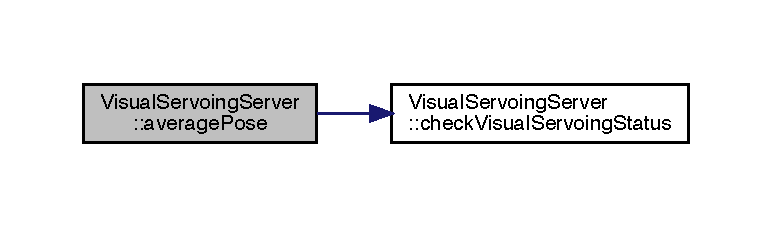
\includegraphics[width=350pt]{classVisualServoingServer_a66e3aaa742d5b0d23a6d3a33a800c088_cgraph}
\end{center}
\end{figure}
\mbox{\Hypertarget{classVisualServoingServer_abe1d3c25e81378f9a1a834d64cf0c496}\label{classVisualServoingServer_abe1d3c25e81378f9a1a834d64cf0c496}} 
\index{Visual\+Servoing\+Server@{Visual\+Servoing\+Server}!backproc\+\_\+\+Update\+Visual\+Servoing\+Paramters@{backproc\+\_\+\+Update\+Visual\+Servoing\+Paramters}}
\index{backproc\+\_\+\+Update\+Visual\+Servoing\+Paramters@{backproc\+\_\+\+Update\+Visual\+Servoing\+Paramters}!Visual\+Servoing\+Server@{Visual\+Servoing\+Server}}
\subsubsection{\texorpdfstring{backproc\+\_\+\+Update\+Visual\+Servoing\+Paramters()}{backproc\_UpdateVisualServoingParamters()}}
{\footnotesize\ttfamily void Visual\+Servoing\+Server\+::backproc\+\_\+\+Update\+Visual\+Servoing\+Paramters (\begin{DoxyParamCaption}{ }\end{DoxyParamCaption})\hspace{0.3cm}{\ttfamily [private]}}



Definition at line 2796 of file Visual\+Servoing\+Server.\+cpp.



Referenced by thread\+Init().

\mbox{\Hypertarget{classVisualServoingServer_a4f23c649522804e21c7e60655a5dad99}\label{classVisualServoingServer_a4f23c649522804e21c7e60655a5dad99}} 
\index{Visual\+Servoing\+Server@{Visual\+Servoing\+Server}!before\+Start@{before\+Start}}
\index{before\+Start@{before\+Start}!Visual\+Servoing\+Server@{Visual\+Servoing\+Server}}
\subsubsection{\texorpdfstring{before\+Start()}{beforeStart()}}
{\footnotesize\ttfamily void Visual\+Servoing\+Server\+::before\+Start (\begin{DoxyParamCaption}{ }\end{DoxyParamCaption})\hspace{0.3cm}{\ttfamily [override]}, {\ttfamily [protected]}}



Definition at line 986 of file Visual\+Servoing\+Server.\+cpp.

\mbox{\Hypertarget{classVisualServoingServer_a9ad2bd94ff95fde9e309c4fb62de7377}\label{classVisualServoingServer_a9ad2bd94ff95fde9e309c4fb62de7377}} 
\index{Visual\+Servoing\+Server@{Visual\+Servoing\+Server}!cartesian\+Position\+Based\+Visual\+Servo\+Control@{cartesian\+Position\+Based\+Visual\+Servo\+Control}}
\index{cartesian\+Position\+Based\+Visual\+Servo\+Control@{cartesian\+Position\+Based\+Visual\+Servo\+Control}!Visual\+Servoing\+Server@{Visual\+Servoing\+Server}}
\subsubsection{\texorpdfstring{cartesian\+Position\+Based\+Visual\+Servo\+Control()}{cartesianPositionBasedVisualServoControl()}}
{\footnotesize\ttfamily void Visual\+Servoing\+Server\+::cartesian\+Position\+Based\+Visual\+Servo\+Control (\begin{DoxyParamCaption}{ }\end{DoxyParamCaption})\hspace{0.3cm}{\ttfamily [private]}}



Definition at line 2071 of file Visual\+Servoing\+Server.\+cpp.

\mbox{\Hypertarget{classVisualServoingServer_a17a9b2913815c52b5a1bd2fd84d9f18e}\label{classVisualServoingServer_a17a9b2913815c52b5a1bd2fd84d9f18e}} 
\index{Visual\+Servoing\+Server@{Visual\+Servoing\+Server}!check\+\_\+visual\+\_\+servoing\+\_\+controller@{check\+\_\+visual\+\_\+servoing\+\_\+controller}}
\index{check\+\_\+visual\+\_\+servoing\+\_\+controller@{check\+\_\+visual\+\_\+servoing\+\_\+controller}!Visual\+Servoing\+Server@{Visual\+Servoing\+Server}}
\subsubsection{\texorpdfstring{check\+\_\+visual\+\_\+servoing\+\_\+controller()}{check\_visual\_servoing\_controller()}}
{\footnotesize\ttfamily bool Visual\+Servoing\+Server\+::check\+\_\+visual\+\_\+servoing\+\_\+controller (\begin{DoxyParamCaption}{ }\end{DoxyParamCaption})\hspace{0.3cm}{\ttfamily [override]}, {\ttfamily [protected]}, {\ttfamily [virtual]}}



Check once whether the visual servoing controller is running or not. 

\begin{DoxyReturn}{Returns}
true/false on it is running/not running. 
\end{DoxyReturn}
\begin{DoxyNote}{Note}
The visual servoing controller may be terminated due to many different reasons, not strictly related to reaching the goal. 
\end{DoxyNote}


Reimplemented from \hyperlink{classVisualServoingIDL_a6426bda1341487c0dbb1f6a048a45deb}{Visual\+Servoing\+I\+DL}.



Definition at line 1220 of file Visual\+Servoing\+Server.\+cpp.

\mbox{\Hypertarget{classVisualServoingServer_afa417f05dd02d2e91ff2c848f082a33b}\label{classVisualServoingServer_afa417f05dd02d2e91ff2c848f082a33b}} 
\index{Visual\+Servoing\+Server@{Visual\+Servoing\+Server}!check\+Visual\+Servoing\+Controller@{check\+Visual\+Servoing\+Controller}}
\index{check\+Visual\+Servoing\+Controller@{check\+Visual\+Servoing\+Controller}!Visual\+Servoing\+Server@{Visual\+Servoing\+Server}}
\subsubsection{\texorpdfstring{check\+Visual\+Servoing\+Controller()}{checkVisualServoingController()}}
{\footnotesize\ttfamily bool Visual\+Servoing\+Server\+::check\+Visual\+Servoing\+Controller (\begin{DoxyParamCaption}{ }\end{DoxyParamCaption})\hspace{0.3cm}{\ttfamily [override]}}



Definition at line 589 of file Visual\+Servoing\+Server.\+cpp.

\mbox{\Hypertarget{classVisualServoingServer_a6201a672d3efe497dd0114df50aee4d7}\label{classVisualServoingServer_a6201a672d3efe497dd0114df50aee4d7}} 
\index{Visual\+Servoing\+Server@{Visual\+Servoing\+Server}!check\+Visual\+Servoing\+Status@{check\+Visual\+Servoing\+Status}}
\index{check\+Visual\+Servoing\+Status@{check\+Visual\+Servoing\+Status}!Visual\+Servoing\+Server@{Visual\+Servoing\+Server}}
\subsubsection{\texorpdfstring{check\+Visual\+Servoing\+Status()}{checkVisualServoingStatus()}\hspace{0.1cm}{\footnotesize\ttfamily [1/2]}}
{\footnotesize\ttfamily bool Visual\+Servoing\+Server\+::check\+Visual\+Servoing\+Status (\begin{DoxyParamCaption}\item[{const yarp\+::sig\+::\+Vector \&}]{px\+\_\+cur,  }\item[{const double}]{tol }\end{DoxyParamCaption})\hspace{0.3cm}{\ttfamily [private]}}



Referenced by average\+Pose().

\mbox{\Hypertarget{classVisualServoingServer_afbcab623f48e3d2e648e144e22df4f19}\label{classVisualServoingServer_afbcab623f48e3d2e648e144e22df4f19}} 
\index{Visual\+Servoing\+Server@{Visual\+Servoing\+Server}!check\+Visual\+Servoing\+Status@{check\+Visual\+Servoing\+Status}}
\index{check\+Visual\+Servoing\+Status@{check\+Visual\+Servoing\+Status}!Visual\+Servoing\+Server@{Visual\+Servoing\+Server}}
\subsubsection{\texorpdfstring{check\+Visual\+Servoing\+Status()}{checkVisualServoingStatus()}\hspace{0.1cm}{\footnotesize\ttfamily [2/2]}}
{\footnotesize\ttfamily bool Visual\+Servoing\+Server\+::check\+Visual\+Servoing\+Status (\begin{DoxyParamCaption}\item[{const yarp\+::sig\+::\+Vector \&}]{pose\+\_\+cur,  }\item[{const double}]{tol\+\_\+position,  }\item[{const double}]{tol\+\_\+orientation,  }\item[{const double}]{tol\+\_\+angle }\end{DoxyParamCaption})\hspace{0.3cm}{\ttfamily [private]}}

\mbox{\Hypertarget{classVisualServoingServer_ad9679d0bc524de74f4e96a1e8be23ca0}\label{classVisualServoingServer_ad9679d0bc524de74f4e96a1e8be23ca0}} 
\index{Visual\+Servoing\+Server@{Visual\+Servoing\+Server}!close@{close}}
\index{close@{close}!Visual\+Servoing\+Server@{Visual\+Servoing\+Server}}
\subsubsection{\texorpdfstring{close()}{close()}}
{\footnotesize\ttfamily bool Visual\+Servoing\+Server\+::close (\begin{DoxyParamCaption}{ }\end{DoxyParamCaption})\hspace{0.3cm}{\ttfamily [override]}}



Definition at line 185 of file Visual\+Servoing\+Server.\+cpp.

\mbox{\Hypertarget{classVisualServoingServer_a79aafac31c32f2028836e1ef0f69dd99}\label{classVisualServoingServer_a79aafac31c32f2028836e1ef0f69dd99}} 
\index{Visual\+Servoing\+Server@{Visual\+Servoing\+Server}!decoupled\+Image\+Based\+Visual\+Servo\+Control@{decoupled\+Image\+Based\+Visual\+Servo\+Control}}
\index{decoupled\+Image\+Based\+Visual\+Servo\+Control@{decoupled\+Image\+Based\+Visual\+Servo\+Control}!Visual\+Servoing\+Server@{Visual\+Servoing\+Server}}
\subsubsection{\texorpdfstring{decoupled\+Image\+Based\+Visual\+Servo\+Control()}{decoupledImageBasedVisualServoControl()}}
{\footnotesize\ttfamily void Visual\+Servoing\+Server\+::decoupled\+Image\+Based\+Visual\+Servo\+Control (\begin{DoxyParamCaption}{ }\end{DoxyParamCaption})\hspace{0.3cm}{\ttfamily [private]}}



Definition at line 1315 of file Visual\+Servoing\+Server.\+cpp.

\mbox{\Hypertarget{classVisualServoingServer_acc8932e08714c503ba6cfda11461976e}\label{classVisualServoingServer_acc8932e08714c503ba6cfda11461976e}} 
\index{Visual\+Servoing\+Server@{Visual\+Servoing\+Server}!get3\+D\+Goal\+Positions\+From3\+D\+Pose@{get3\+D\+Goal\+Positions\+From3\+D\+Pose}}
\index{get3\+D\+Goal\+Positions\+From3\+D\+Pose@{get3\+D\+Goal\+Positions\+From3\+D\+Pose}!Visual\+Servoing\+Server@{Visual\+Servoing\+Server}}
\subsubsection{\texorpdfstring{get3\+D\+Goal\+Positions\+From3\+D\+Pose()}{get3DGoalPositionsFrom3DPose()}}
{\footnotesize\ttfamily std\+::vector$<$ Vector $>$ Visual\+Servoing\+Server\+::get3\+D\+Goal\+Positions\+From3\+D\+Pose (\begin{DoxyParamCaption}\item[{const yarp\+::sig\+::\+Vector \&}]{x,  }\item[{const yarp\+::sig\+::\+Vector \&}]{o }\end{DoxyParamCaption})\hspace{0.3cm}{\ttfamily [override]}}



Definition at line 675 of file Visual\+Servoing\+Server.\+cpp.

\mbox{\Hypertarget{classVisualServoingServer_a542e0a6bf6158563a601740363911474}\label{classVisualServoingServer_a542e0a6bf6158563a601740363911474}} 
\index{Visual\+Servoing\+Server@{Visual\+Servoing\+Server}!get\+\_\+3\+D\+\_\+goal\+\_\+positions\+\_\+from\+\_\+3\+D\+\_\+pose@{get\+\_\+3\+D\+\_\+goal\+\_\+positions\+\_\+from\+\_\+3\+D\+\_\+pose}}
\index{get\+\_\+3\+D\+\_\+goal\+\_\+positions\+\_\+from\+\_\+3\+D\+\_\+pose@{get\+\_\+3\+D\+\_\+goal\+\_\+positions\+\_\+from\+\_\+3\+D\+\_\+pose}!Visual\+Servoing\+Server@{Visual\+Servoing\+Server}}
\subsubsection{\texorpdfstring{get\+\_\+3\+D\+\_\+goal\+\_\+positions\+\_\+from\+\_\+3\+D\+\_\+pose()}{get\_3D\_goal\_positions\_from\_3D\_pose()}}
{\footnotesize\ttfamily std\+::vector$<$ std\+::vector$<$ double $>$ $>$ Visual\+Servoing\+Server\+::get\+\_\+3\+D\+\_\+goal\+\_\+positions\+\_\+from\+\_\+3\+D\+\_\+pose (\begin{DoxyParamCaption}\item[{const std\+::vector$<$ double $>$ \&}]{x,  }\item[{const std\+::vector$<$ double $>$ \&}]{o }\end{DoxyParamCaption})\hspace{0.3cm}{\ttfamily [override]}, {\ttfamily [protected]}, {\ttfamily [virtual]}}



Helper function\+: extract four Cartesian points lying on the plane defined by the frame o in the position x relative to the robot base frame. 


\begin{DoxyParams}{Parameters}
{\em x} & a 3D vector which is filled with the actual position (x, y, z) \mbox{[}m\mbox{]}. \\
\hline
{\em o} & a 4D vector which is filled with the actual orientation using axis-\/angle representation (xa, ya, za) and (theta) \mbox{[}rad\mbox{]}. \\
\hline
\end{DoxyParams}
\begin{DoxyReturn}{Returns}
on success\+: a collection of four Cartesian points (position only) extracted from the plane defined by x and o; on failure\+: an empty list. 
\end{DoxyReturn}
\begin{DoxyNote}{Note}
It is always suggested to check whether the returned list is empty or not and to take proper counter actions. 
\end{DoxyNote}


Reimplemented from \hyperlink{classVisualServoingIDL_a175b2d3fb77000e0012c7a8d16e9a379}{Visual\+Servoing\+I\+DL}.



Definition at line 1274 of file Visual\+Servoing\+Server.\+cpp.

\mbox{\Hypertarget{classVisualServoingServer_a3b0e5078c2f32493a2ef31ea32450d80}\label{classVisualServoingServer_a3b0e5078c2f32493a2ef31ea32450d80}} 
\index{Visual\+Servoing\+Server@{Visual\+Servoing\+Server}!get\+\_\+goal\+\_\+from\+\_\+sfm@{get\+\_\+goal\+\_\+from\+\_\+sfm}}
\index{get\+\_\+goal\+\_\+from\+\_\+sfm@{get\+\_\+goal\+\_\+from\+\_\+sfm}!Visual\+Servoing\+Server@{Visual\+Servoing\+Server}}
\subsubsection{\texorpdfstring{get\+\_\+goal\+\_\+from\+\_\+sfm()}{get\_goal\_from\_sfm()}}
{\footnotesize\ttfamily bool Visual\+Servoing\+Server\+::get\+\_\+goal\+\_\+from\+\_\+sfm (\begin{DoxyParamCaption}{ }\end{DoxyParamCaption})\hspace{0.3cm}{\ttfamily [override]}, {\ttfamily [protected]}, {\ttfamily [virtual]}}



Get goal point from S\+FM module. 

The point is taken by clicking on a dedicated \textquotesingle{}yarpview\textquotesingle{} G\+UI and the orientation is hard-\/coded. \begin{DoxyNote}{Note}
This service is experimental and should be used with care. 
\end{DoxyNote}
\begin{DoxyReturn}{Returns}
true upon success, false otherwise. 
\end{DoxyReturn}


Reimplemented from \hyperlink{classVisualServoingIDL_aff8af7d3ebe68f5fbfa7197eb7115723}{Visual\+Servoing\+I\+DL}.



Definition at line 1099 of file Visual\+Servoing\+Server.\+cpp.

\mbox{\Hypertarget{classVisualServoingServer_aaa84d7964120ee1056f422dc2d5eb070}\label{classVisualServoingServer_aaa84d7964120ee1056f422dc2d5eb070}} 
\index{Visual\+Servoing\+Server@{Visual\+Servoing\+Server}!get\+\_\+goal\+\_\+pixels\+\_\+from\+\_\+3\+D\+\_\+pose@{get\+\_\+goal\+\_\+pixels\+\_\+from\+\_\+3\+D\+\_\+pose}}
\index{get\+\_\+goal\+\_\+pixels\+\_\+from\+\_\+3\+D\+\_\+pose@{get\+\_\+goal\+\_\+pixels\+\_\+from\+\_\+3\+D\+\_\+pose}!Visual\+Servoing\+Server@{Visual\+Servoing\+Server}}
\subsubsection{\texorpdfstring{get\+\_\+goal\+\_\+pixels\+\_\+from\+\_\+3\+D\+\_\+pose()}{get\_goal\_pixels\_from\_3D\_pose()}}
{\footnotesize\ttfamily std\+::vector$<$ std\+::vector$<$ double $>$ $>$ Visual\+Servoing\+Server\+::get\+\_\+goal\+\_\+pixels\+\_\+from\+\_\+3\+D\+\_\+pose (\begin{DoxyParamCaption}\item[{const std\+::vector$<$ double $>$ \&}]{x,  }\item[{const std\+::vector$<$ double $>$ \&}]{o,  }\item[{const std\+::string \&}]{cam }\end{DoxyParamCaption})\hspace{0.3cm}{\ttfamily [override]}, {\ttfamily [protected]}, {\ttfamily [virtual]}}



Helper function\+: extract four 2D pixel points lying on the plane defined by the frame o in the position x relative to the robot base frame. 


\begin{DoxyParams}{Parameters}
{\em x} & a 3D vector which is filled with the actual position (x, y, z) \mbox{[}m\mbox{]}. \\
\hline
{\em o} & a 4D vector which is filled with the actual orientation using axis-\/angle representation (xa, ya, za) and (theta) \mbox{[}m\mbox{]}/\mbox{[}rad\mbox{]}. \\
\hline
{\em cam} & either \char`\"{}left\char`\"{} or \char`\"{}right\char`\"{} to select left or right camera. \\
\hline
\end{DoxyParams}
\begin{DoxyReturn}{Returns}
on success\+: a collection of three (u, v) pixel points extracted from the plane defined by x and o; on failure\+: an empty list. 
\end{DoxyReturn}
\begin{DoxyNote}{Note}
It is always suggested to check whether the returned list is empty or not and to take proper counter actions. 
\end{DoxyNote}


Reimplemented from \hyperlink{classVisualServoingIDL_afb359486a7e42bfda3ddf66a2e518e90}{Visual\+Servoing\+I\+DL}.



Definition at line 1292 of file Visual\+Servoing\+Server.\+cpp.

\mbox{\Hypertarget{classVisualServoingServer_af085e2c5d4c4cfe940b3564b4ba69af6}\label{classVisualServoingServer_af085e2c5d4c4cfe940b3564b4ba69af6}} 
\index{Visual\+Servoing\+Server@{Visual\+Servoing\+Server}!get\+\_\+visual\+\_\+servoing\+\_\+info@{get\+\_\+visual\+\_\+servoing\+\_\+info}}
\index{get\+\_\+visual\+\_\+servoing\+\_\+info@{get\+\_\+visual\+\_\+servoing\+\_\+info}!Visual\+Servoing\+Server@{Visual\+Servoing\+Server}}
\subsubsection{\texorpdfstring{get\+\_\+visual\+\_\+servoing\+\_\+info()}{get\_visual\_servoing\_info()}}
{\footnotesize\ttfamily std\+::vector$<$ std\+::string $>$ Visual\+Servoing\+Server\+::get\+\_\+visual\+\_\+servoing\+\_\+info (\begin{DoxyParamCaption}{ }\end{DoxyParamCaption})\hspace{0.3cm}{\ttfamily [override]}, {\ttfamily [protected]}, {\ttfamily [virtual]}}



Return useful information for visual servoing. 

\begin{DoxyReturn}{Returns}
All the visual servoing information. 
\end{DoxyReturn}


Reimplemented from \hyperlink{classVisualServoingIDL_a9654ec3984d53b41f50e0d70b2991203}{Visual\+Servoing\+I\+DL}.



Definition at line 1202 of file Visual\+Servoing\+Server.\+cpp.

\mbox{\Hypertarget{classVisualServoingServer_a43cf45e933a71214cfb4d8248005761e}\label{classVisualServoingServer_a43cf45e933a71214cfb4d8248005761e}} 
\index{Visual\+Servoing\+Server@{Visual\+Servoing\+Server}!get\+Control\+Pixel\+From\+Point@{get\+Control\+Pixel\+From\+Point}}
\index{get\+Control\+Pixel\+From\+Point@{get\+Control\+Pixel\+From\+Point}!Visual\+Servoing\+Server@{Visual\+Servoing\+Server}}
\subsubsection{\texorpdfstring{get\+Control\+Pixel\+From\+Point()}{getControlPixelFromPoint()}}
{\footnotesize\ttfamily Vector Visual\+Servoing\+Server\+::get\+Control\+Pixel\+From\+Point (\begin{DoxyParamCaption}\item[{const Cam\+Sel \&}]{cam,  }\item[{const yarp\+::sig\+::\+Vector \&}]{p }\end{DoxyParamCaption}) const\hspace{0.3cm}{\ttfamily [private]}}



Definition at line 2626 of file Visual\+Servoing\+Server.\+cpp.

\mbox{\Hypertarget{classVisualServoingServer_a67bfc714271a28bf55fa49c89019b53c}\label{classVisualServoingServer_a67bfc714271a28bf55fa49c89019b53c}} 
\index{Visual\+Servoing\+Server@{Visual\+Servoing\+Server}!get\+Control\+Pixels\+From\+Pose@{get\+Control\+Pixels\+From\+Pose}}
\index{get\+Control\+Pixels\+From\+Pose@{get\+Control\+Pixels\+From\+Pose}!Visual\+Servoing\+Server@{Visual\+Servoing\+Server}}
\subsubsection{\texorpdfstring{get\+Control\+Pixels\+From\+Pose()}{getControlPixelsFromPose()}}
{\footnotesize\ttfamily std\+::vector$<$ Vector $>$ Visual\+Servoing\+Server\+::get\+Control\+Pixels\+From\+Pose (\begin{DoxyParamCaption}\item[{const yarp\+::sig\+::\+Vector \&}]{pose,  }\item[{const Cam\+Sel \&}]{cam,  }\item[{const \hyperlink{classVisualServoingServer_a3a1cce02f57cebb9056da5653d4dff0e}{Pixel\+Control\+Mode} \&}]{mode }\end{DoxyParamCaption})\hspace{0.3cm}{\ttfamily [private]}}



Definition at line 2553 of file Visual\+Servoing\+Server.\+cpp.

\mbox{\Hypertarget{classVisualServoingServer_ac9e6020f30b6df05db3fc34a44fee0d4}\label{classVisualServoingServer_ac9e6020f30b6df05db3fc34a44fee0d4}} 
\index{Visual\+Servoing\+Server@{Visual\+Servoing\+Server}!get\+Control\+Points\+From\+Pose@{get\+Control\+Points\+From\+Pose}}
\index{get\+Control\+Points\+From\+Pose@{get\+Control\+Points\+From\+Pose}!Visual\+Servoing\+Server@{Visual\+Servoing\+Server}}
\subsubsection{\texorpdfstring{get\+Control\+Points\+From\+Pose()}{getControlPointsFromPose()}}
{\footnotesize\ttfamily std\+::vector$<$ Vector $>$ Visual\+Servoing\+Server\+::get\+Control\+Points\+From\+Pose (\begin{DoxyParamCaption}\item[{const yarp\+::sig\+::\+Vector \&}]{pose }\end{DoxyParamCaption})\hspace{0.3cm}{\ttfamily [private]}}



Definition at line 2576 of file Visual\+Servoing\+Server.\+cpp.

\mbox{\Hypertarget{classVisualServoingServer_ad5334ed717f373cfbd40290824d9ed1f}\label{classVisualServoingServer_ad5334ed717f373cfbd40290824d9ed1f}} 
\index{Visual\+Servoing\+Server@{Visual\+Servoing\+Server}!get\+Current\+Stereo\+Features\+And\+Jacobian@{get\+Current\+Stereo\+Features\+And\+Jacobian}}
\index{get\+Current\+Stereo\+Features\+And\+Jacobian@{get\+Current\+Stereo\+Features\+And\+Jacobian}!Visual\+Servoing\+Server@{Visual\+Servoing\+Server}}
\subsubsection{\texorpdfstring{get\+Current\+Stereo\+Features\+And\+Jacobian()}{getCurrentStereoFeaturesAndJacobian()}}
{\footnotesize\ttfamily void Visual\+Servoing\+Server\+::get\+Current\+Stereo\+Features\+And\+Jacobian (\begin{DoxyParamCaption}\item[{const std\+::vector$<$ yarp\+::sig\+::\+Vector $>$ \&}]{left\+\_\+px,  }\item[{const std\+::vector$<$ yarp\+::sig\+::\+Vector $>$ \&}]{right\+\_\+px,  }\item[{yarp\+::sig\+::\+Vector \&}]{features,  }\item[{yarp\+::sig\+::\+Matrix \&}]{jacobian }\end{DoxyParamCaption})\hspace{0.3cm}{\ttfamily [private]}}



Definition at line 2646 of file Visual\+Servoing\+Server.\+cpp.

\mbox{\Hypertarget{classVisualServoingServer_a9d35a09c55cc8c059dc7bdbeeed8cfb1}\label{classVisualServoingServer_a9d35a09c55cc8c059dc7bdbeeed8cfb1}} 
\index{Visual\+Servoing\+Server@{Visual\+Servoing\+Server}!get\+Goal\+Pixels\+From3\+D\+Pose@{get\+Goal\+Pixels\+From3\+D\+Pose}}
\index{get\+Goal\+Pixels\+From3\+D\+Pose@{get\+Goal\+Pixels\+From3\+D\+Pose}!Visual\+Servoing\+Server@{Visual\+Servoing\+Server}}
\subsubsection{\texorpdfstring{get\+Goal\+Pixels\+From3\+D\+Pose()}{getGoalPixelsFrom3DPose()}}
{\footnotesize\ttfamily std\+::vector$<$ Vector $>$ Visual\+Servoing\+Server\+::get\+Goal\+Pixels\+From3\+D\+Pose (\begin{DoxyParamCaption}\item[{const yarp\+::sig\+::\+Vector \&}]{x,  }\item[{const yarp\+::sig\+::\+Vector \&}]{o,  }\item[{const Cam\+Sel \&}]{cam }\end{DoxyParamCaption})\hspace{0.3cm}{\ttfamily [override]}}



Definition at line 695 of file Visual\+Servoing\+Server.\+cpp.

\mbox{\Hypertarget{classVisualServoingServer_a3aa225c2c4f417c4ea7dd27e9b6d0c8a}\label{classVisualServoingServer_a3aa225c2c4f417c4ea7dd27e9b6d0c8a}} 
\index{Visual\+Servoing\+Server@{Visual\+Servoing\+Server}!get\+JacobianU@{get\+JacobianU}}
\index{get\+JacobianU@{get\+JacobianU}!Visual\+Servoing\+Server@{Visual\+Servoing\+Server}}
\subsubsection{\texorpdfstring{get\+Jacobian\+U()}{getJacobianU()}}
{\footnotesize\ttfamily Vector Visual\+Servoing\+Server\+::get\+JacobianU (\begin{DoxyParamCaption}\item[{const Cam\+Sel \&}]{cam,  }\item[{const yarp\+::sig\+::\+Vector \&}]{px }\end{DoxyParamCaption})\hspace{0.3cm}{\ttfamily [private]}}



Definition at line 2685 of file Visual\+Servoing\+Server.\+cpp.

\mbox{\Hypertarget{classVisualServoingServer_a51667642f6d882df082f79ec01111181}\label{classVisualServoingServer_a51667642f6d882df082f79ec01111181}} 
\index{Visual\+Servoing\+Server@{Visual\+Servoing\+Server}!get\+JacobianV@{get\+JacobianV}}
\index{get\+JacobianV@{get\+JacobianV}!Visual\+Servoing\+Server@{Visual\+Servoing\+Server}}
\subsubsection{\texorpdfstring{get\+Jacobian\+V()}{getJacobianV()}}
{\footnotesize\ttfamily Vector Visual\+Servoing\+Server\+::get\+JacobianV (\begin{DoxyParamCaption}\item[{const Cam\+Sel \&}]{cam,  }\item[{const yarp\+::sig\+::\+Vector \&}]{px }\end{DoxyParamCaption})\hspace{0.3cm}{\ttfamily [private]}}



Definition at line 2710 of file Visual\+Servoing\+Server.\+cpp.

\mbox{\Hypertarget{classVisualServoingServer_a997029621c723c1e9962b35a917167cc}\label{classVisualServoingServer_a997029621c723c1e9962b35a917167cc}} 
\index{Visual\+Servoing\+Server@{Visual\+Servoing\+Server}!get\+Pixel\+From\+Point@{get\+Pixel\+From\+Point}}
\index{get\+Pixel\+From\+Point@{get\+Pixel\+From\+Point}!Visual\+Servoing\+Server@{Visual\+Servoing\+Server}}
\subsubsection{\texorpdfstring{get\+Pixel\+From\+Point()}{getPixelFromPoint()}}
{\footnotesize\ttfamily Vector Visual\+Servoing\+Server\+::get\+Pixel\+From\+Point (\begin{DoxyParamCaption}\item[{const Cam\+Sel \&}]{cam,  }\item[{const yarp\+::sig\+::\+Vector \&}]{p }\end{DoxyParamCaption}) const\hspace{0.3cm}{\ttfamily [private]}}



Definition at line 2620 of file Visual\+Servoing\+Server.\+cpp.

\mbox{\Hypertarget{classVisualServoingServer_a04f3caed0ac350b3579efeb4cd548eb8}\label{classVisualServoingServer_a04f3caed0ac350b3579efeb4cd548eb8}} 
\index{Visual\+Servoing\+Server@{Visual\+Servoing\+Server}!get\+Pixels\+From\+Pose@{get\+Pixels\+From\+Pose}}
\index{get\+Pixels\+From\+Pose@{get\+Pixels\+From\+Pose}!Visual\+Servoing\+Server@{Visual\+Servoing\+Server}}
\subsubsection{\texorpdfstring{get\+Pixels\+From\+Pose()}{getPixelsFromPose()}}
{\footnotesize\ttfamily std\+::vector$<$ Vector $>$ Visual\+Servoing\+Server\+::get\+Pixels\+From\+Pose (\begin{DoxyParamCaption}\item[{const yarp\+::sig\+::\+Vector \&}]{pose,  }\item[{const Cam\+Sel \&}]{cam }\end{DoxyParamCaption})\hspace{0.3cm}{\ttfamily [private]}}



Definition at line 2537 of file Visual\+Servoing\+Server.\+cpp.

\mbox{\Hypertarget{classVisualServoingServer_a66db1dfa1ebde34ada94bc36248e2ec8}\label{classVisualServoingServer_a66db1dfa1ebde34ada94bc36248e2ec8}} 
\index{Visual\+Servoing\+Server@{Visual\+Servoing\+Server}!get\+Visual\+Servoing\+Info@{get\+Visual\+Servoing\+Info}}
\index{get\+Visual\+Servoing\+Info@{get\+Visual\+Servoing\+Info}!Visual\+Servoing\+Server@{Visual\+Servoing\+Server}}
\subsubsection{\texorpdfstring{get\+Visual\+Servoing\+Info()}{getVisualServoingInfo()}}
{\footnotesize\ttfamily bool Visual\+Servoing\+Server\+::get\+Visual\+Servoing\+Info (\begin{DoxyParamCaption}\item[{yarp\+::os\+::\+Bottle \&}]{info }\end{DoxyParamCaption})\hspace{0.3cm}{\ttfamily [override]}}



Definition at line 573 of file Visual\+Servoing\+Server.\+cpp.

\mbox{\Hypertarget{classVisualServoingServer_a77f26ac40c67d7a9b7e4ad7840532681}\label{classVisualServoingServer_a77f26ac40c67d7a9b7e4ad7840532681}} 
\index{Visual\+Servoing\+Server@{Visual\+Servoing\+Server}!go\+\_\+to\+\_\+pose\+\_\+goal@{go\+\_\+to\+\_\+pose\+\_\+goal}}
\index{go\+\_\+to\+\_\+pose\+\_\+goal@{go\+\_\+to\+\_\+pose\+\_\+goal}!Visual\+Servoing\+Server@{Visual\+Servoing\+Server}}
\subsubsection{\texorpdfstring{go\+\_\+to\+\_\+pose\+\_\+goal()}{go\_to\_pose\_goal()}}
{\footnotesize\ttfamily bool Visual\+Servoing\+Server\+::go\+\_\+to\+\_\+pose\+\_\+goal (\begin{DoxyParamCaption}\item[{const std\+::vector$<$ double $>$ \&}]{vec\+\_\+x,  }\item[{const std\+::vector$<$ double $>$ \&}]{vec\+\_\+o }\end{DoxyParamCaption})\hspace{0.3cm}{\ttfamily [override]}, {\ttfamily [protected]}, {\ttfamily [virtual]}}



Set the goal point (3D for the position + 4D axis-\/angle for the orientation) and start visual servoing. 


\begin{DoxyParams}{Parameters}
{\em vec\+\_\+x} & a 3D vector which contains the (x, y, z) Cartesian coordinates of the goal. \\
\hline
{\em vec\+\_\+o} & a 4D vector which contains the (x, y, z) axis and theta angle of rotation of the goal. \\
\hline
\end{DoxyParams}
\begin{DoxyNote}{Note}
By invoking this method, the visual servoing goal will be reached in position and orientation together with two parallel tasks. 
\end{DoxyNote}
\begin{DoxyReturn}{Returns}
true/false on success/failure. 
\end{DoxyReturn}


Reimplemented from \hyperlink{classVisualServoingIDL_a697368ff5a1b3f16069d1d10f25ca888}{Visual\+Servoing\+I\+DL}.



Definition at line 1172 of file Visual\+Servoing\+Server.\+cpp.

\mbox{\Hypertarget{classVisualServoingIDL_a75929f915651161c43ed032e9f69a361}\label{classVisualServoingIDL_a75929f915651161c43ed032e9f69a361}} 
\index{Visual\+Servoing\+Server@{Visual\+Servoing\+Server}!go\+\_\+to\+\_\+px\+\_\+goal@{go\+\_\+to\+\_\+px\+\_\+goal}}
\index{go\+\_\+to\+\_\+px\+\_\+goal@{go\+\_\+to\+\_\+px\+\_\+goal}!Visual\+Servoing\+Server@{Visual\+Servoing\+Server}}
\subsubsection{\texorpdfstring{go\+\_\+to\+\_\+px\+\_\+goal()}{go\_to\_px\_goal()}\hspace{0.1cm}{\footnotesize\ttfamily [1/2]}}
{\footnotesize\ttfamily virtual bool Visual\+Servoing\+I\+D\+L\+::go\+\_\+to\+\_\+px\+\_\+goal (\begin{DoxyParamCaption}\item[{const std\+::vector$<$ std\+::vector$<$ double $>$ $>$ \&}]{vec\+\_\+px\+\_\+l,  }\item[{const std\+::vector$<$ std\+::vector$<$ double $>$ $>$ \&}]{vec\+\_\+px\+\_\+r }\end{DoxyParamCaption})\hspace{0.3cm}{\ttfamily [virtual]}, {\ttfamily [inherited]}}



Set the goal points on both left and right camera image plane and start visual servoing. 


\begin{DoxyParams}{Parameters}
{\em vec\+\_\+px\+\_\+l} & a collection of four 2D vectors which contains the (u, v) coordinates of the pixels within the left image plane. \\
\hline
{\em vec\+\_\+px\+\_\+r} & a collection of four 2D vectors which contains the (u, v) coordinates of the pixels within the right image plane. \\
\hline
\end{DoxyParams}
\begin{DoxyNote}{Note}
By invoking this method, the visual servoing goal will be reached in orientation first, then in position. This is because there may not be a feasible position solution for every possible orientation. 
\end{DoxyNote}
\begin{DoxyReturn}{Returns}
true/false on success/failure. 
\end{DoxyReturn}
\mbox{\Hypertarget{classVisualServoingServer_a6b68da9fe211a5779fc7a24e406dc8f0}\label{classVisualServoingServer_a6b68da9fe211a5779fc7a24e406dc8f0}} 
\index{Visual\+Servoing\+Server@{Visual\+Servoing\+Server}!go\+\_\+to\+\_\+px\+\_\+goal@{go\+\_\+to\+\_\+px\+\_\+goal}}
\index{go\+\_\+to\+\_\+px\+\_\+goal@{go\+\_\+to\+\_\+px\+\_\+goal}!Visual\+Servoing\+Server@{Visual\+Servoing\+Server}}
\subsubsection{\texorpdfstring{go\+\_\+to\+\_\+px\+\_\+goal()}{go\_to\_px\_goal()}\hspace{0.1cm}{\footnotesize\ttfamily [2/2]}}
{\footnotesize\ttfamily bool Visual\+Servoing\+Server\+::go\+\_\+to\+\_\+px\+\_\+goal (\begin{DoxyParamCaption}\item[{const std\+::vector$<$ std\+::vector$<$ double $>$$>$ \&}]{vec\+\_\+px\+\_\+l,  }\item[{const std\+::vector$<$ std\+::vector$<$ double $>$$>$ \&}]{vec\+\_\+px\+\_\+r }\end{DoxyParamCaption})\hspace{0.3cm}{\ttfamily [override]}, {\ttfamily [protected]}}



Definition at line 1145 of file Visual\+Servoing\+Server.\+cpp.

\mbox{\Hypertarget{classVisualServoingServer_a085bb298e50f295d670bff6e4cb808d8}\label{classVisualServoingServer_a085bb298e50f295d670bff6e4cb808d8}} 
\index{Visual\+Servoing\+Server@{Visual\+Servoing\+Server}!go\+To\+Goal@{go\+To\+Goal}}
\index{go\+To\+Goal@{go\+To\+Goal}!Visual\+Servoing\+Server@{Visual\+Servoing\+Server}}
\subsubsection{\texorpdfstring{go\+To\+Goal()}{goToGoal()}\hspace{0.1cm}{\footnotesize\ttfamily [1/2]}}
{\footnotesize\ttfamily bool Visual\+Servoing\+Server\+::go\+To\+Goal (\begin{DoxyParamCaption}\item[{const yarp\+::sig\+::\+Vector \&}]{vec\+\_\+x,  }\item[{const yarp\+::sig\+::\+Vector \&}]{vec\+\_\+o }\end{DoxyParamCaption})\hspace{0.3cm}{\ttfamily [override]}}



Referenced by stop\+Facilities().

\mbox{\Hypertarget{classVisualServoingServer_a40ab9e9804793a58243077f31a2d79a4}\label{classVisualServoingServer_a40ab9e9804793a58243077f31a2d79a4}} 
\index{Visual\+Servoing\+Server@{Visual\+Servoing\+Server}!go\+To\+Goal@{go\+To\+Goal}}
\index{go\+To\+Goal@{go\+To\+Goal}!Visual\+Servoing\+Server@{Visual\+Servoing\+Server}}
\subsubsection{\texorpdfstring{go\+To\+Goal()}{goToGoal()}\hspace{0.1cm}{\footnotesize\ttfamily [2/2]}}
{\footnotesize\ttfamily bool Visual\+Servoing\+Server\+::go\+To\+Goal (\begin{DoxyParamCaption}\item[{const std\+::vector$<$ yarp\+::sig\+::\+Vector $>$ \&}]{vec\+\_\+px\+\_\+l,  }\item[{const std\+::vector$<$ yarp\+::sig\+::\+Vector $>$ \&}]{vec\+\_\+px\+\_\+r }\end{DoxyParamCaption})\hspace{0.3cm}{\ttfamily [override]}}

\mbox{\Hypertarget{classVisualServoingServer_a6d051da5da8c07b0e0879d5af50a248f}\label{classVisualServoingServer_a6d051da5da8c07b0e0879d5af50a248f}} 
\index{Visual\+Servoing\+Server@{Visual\+Servoing\+Server}!go\+To\+S\+F\+M\+Goal@{go\+To\+S\+F\+M\+Goal}}
\index{go\+To\+S\+F\+M\+Goal@{go\+To\+S\+F\+M\+Goal}!Visual\+Servoing\+Server@{Visual\+Servoing\+Server}}
\subsubsection{\texorpdfstring{go\+To\+S\+F\+M\+Goal()}{goToSFMGoal()}}
{\footnotesize\ttfamily bool Visual\+Servoing\+Server\+::go\+To\+S\+F\+M\+Goal (\begin{DoxyParamCaption}{ }\end{DoxyParamCaption})\hspace{0.3cm}{\ttfamily [override]}}



Definition at line 925 of file Visual\+Servoing\+Server.\+cpp.

\mbox{\Hypertarget{classVisualServoingIDL_a99974ef8858179f14e2762c2d7bf4ed5}\label{classVisualServoingIDL_a99974ef8858179f14e2762c2d7bf4ed5}} 
\index{Visual\+Servoing\+Server@{Visual\+Servoing\+Server}!help@{help}}
\index{help@{help}!Visual\+Servoing\+Server@{Visual\+Servoing\+Server}}
\subsubsection{\texorpdfstring{help()}{help()}}
{\footnotesize\ttfamily virtual std\+::vector$<$std\+::string$>$ Visual\+Servoing\+I\+D\+L\+::help (\begin{DoxyParamCaption}\item[{const std\+::string \&}]{function\+Name = {\ttfamily \char`\"{}-\/-\/all\char`\"{}} }\end{DoxyParamCaption})\hspace{0.3cm}{\ttfamily [virtual]}, {\ttfamily [inherited]}}

\mbox{\Hypertarget{classVisualServoingServer_ad3668e0fc8818f9d2827bbc50087d353}\label{classVisualServoingServer_ad3668e0fc8818f9d2827bbc50087d353}} 
\index{Visual\+Servoing\+Server@{Visual\+Servoing\+Server}!init\+\_\+facilities@{init\+\_\+facilities}}
\index{init\+\_\+facilities@{init\+\_\+facilities}!Visual\+Servoing\+Server@{Visual\+Servoing\+Server}}
\subsubsection{\texorpdfstring{init\+\_\+facilities()}{init\_facilities()}}
{\footnotesize\ttfamily bool Visual\+Servoing\+Server\+::init\+\_\+facilities (\begin{DoxyParamCaption}\item[{const bool}]{use\+\_\+direct\+\_\+kin }\end{DoxyParamCaption})\hspace{0.3cm}{\ttfamily [override]}, {\ttfamily [protected]}, {\ttfamily [virtual]}}



Initialize support modules and connections to perform a visual servoing task. 

This method must be called before any other visual servoing methods. Returns upon successful or failure setup. 
\begin{DoxyParams}{Parameters}
{\em use\+\_\+direct\+\_\+kin} & instruct the visual servoing control to either use direct kinematic or an estimated/refined pose of the end-\/effector. \\
\hline
\end{DoxyParams}
\begin{DoxyNote}{Note}
Default value\+: false. There usually is an error in the robot direct kinematics that should be compensated to perform precise visual servoing. To this end, a recursive Bayesian estimation filter is used to compensate for this error. Such filter is initialized during initialization execution. 
\end{DoxyNote}
\begin{DoxyReturn}{Returns}
true/false on success/failure. 
\end{DoxyReturn}


Reimplemented from \hyperlink{classVisualServoingIDL_aae4ee4c07b50956396fd59bbb00fd9c7}{Visual\+Servoing\+I\+DL}.



Definition at line 1127 of file Visual\+Servoing\+Server.\+cpp.

\mbox{\Hypertarget{classVisualServoingServer_a136cfac8840eda92c012851149b8624a}\label{classVisualServoingServer_a136cfac8840eda92c012851149b8624a}} 
\index{Visual\+Servoing\+Server@{Visual\+Servoing\+Server}!init\+Facilities@{init\+Facilities}}
\index{init\+Facilities@{init\+Facilities}!Visual\+Servoing\+Server@{Visual\+Servoing\+Server}}
\subsubsection{\texorpdfstring{init\+Facilities()}{initFacilities()}}
{\footnotesize\ttfamily bool Visual\+Servoing\+Server\+::init\+Facilities (\begin{DoxyParamCaption}\item[{const bool}]{use\+\_\+direct\+\_\+kin }\end{DoxyParamCaption})\hspace{0.3cm}{\ttfamily [override]}}



Definition at line 253 of file Visual\+Servoing\+Server.\+cpp.

\mbox{\Hypertarget{classVisualServoingServer_a1401f7ee34d88728dd103439b25f9cf5}\label{classVisualServoingServer_a1401f7ee34d88728dd103439b25f9cf5}} 
\index{Visual\+Servoing\+Server@{Visual\+Servoing\+Server}!on\+Stop@{on\+Stop}}
\index{on\+Stop@{on\+Stop}!Visual\+Servoing\+Server@{Visual\+Servoing\+Server}}
\subsubsection{\texorpdfstring{on\+Stop()}{onStop()}}
{\footnotesize\ttfamily void Visual\+Servoing\+Server\+::on\+Stop (\begin{DoxyParamCaption}{ }\end{DoxyParamCaption})\hspace{0.3cm}{\ttfamily [override]}, {\ttfamily [protected]}}



Definition at line 1051 of file Visual\+Servoing\+Server.\+cpp.

\mbox{\Hypertarget{classVisualServoingServer_a0698977ddac02801eba3c35b47b9aa19}\label{classVisualServoingServer_a0698977ddac02801eba3c35b47b9aa19}} 
\index{Visual\+Servoing\+Server@{Visual\+Servoing\+Server}!open@{open}}
\index{open@{open}!Visual\+Servoing\+Server@{Visual\+Servoing\+Server}}
\subsubsection{\texorpdfstring{open()}{open()}}
{\footnotesize\ttfamily bool Visual\+Servoing\+Server\+::open (\begin{DoxyParamCaption}\item[{yarp\+::os\+::\+Searchable \&}]{config }\end{DoxyParamCaption})\hspace{0.3cm}{\ttfamily [override]}}



Definition at line 35 of file Visual\+Servoing\+Server.\+cpp.

\mbox{\Hypertarget{classVisualServoingServer_ac438c7abfb838df458f85e250ead3222}\label{classVisualServoingServer_ac438c7abfb838df458f85e250ead3222}} 
\index{Visual\+Servoing\+Server@{Visual\+Servoing\+Server}!quit@{quit}}
\index{quit@{quit}!Visual\+Servoing\+Server@{Visual\+Servoing\+Server}}
\subsubsection{\texorpdfstring{quit()}{quit()}}
{\footnotesize\ttfamily bool Visual\+Servoing\+Server\+::quit (\begin{DoxyParamCaption}{ }\end{DoxyParamCaption})\hspace{0.3cm}{\ttfamily [override]}, {\ttfamily [protected]}, {\ttfamily [virtual]}}



Gently close the visual servoing device, deallocating resources. 



Reimplemented from \hyperlink{classVisualServoingIDL_a3d5503e1d4bb2b25a11cbd5357b3013b}{Visual\+Servoing\+I\+DL}.



Definition at line 1105 of file Visual\+Servoing\+Server.\+cpp.

\mbox{\Hypertarget{classVisualServoingIDL_a97106bf829447896de03680d78b960a5}\label{classVisualServoingIDL_a97106bf829447896de03680d78b960a5}} 
\index{Visual\+Servoing\+Server@{Visual\+Servoing\+Server}!read@{read}}
\index{read@{read}!Visual\+Servoing\+Server@{Visual\+Servoing\+Server}}
\subsubsection{\texorpdfstring{read()}{read()}}
{\footnotesize\ttfamily virtual bool Visual\+Servoing\+I\+D\+L\+::read (\begin{DoxyParamCaption}\item[{yarp\+::os\+::\+Connection\+Reader \&}]{connection }\end{DoxyParamCaption})\hspace{0.3cm}{\ttfamily [override]}, {\ttfamily [virtual]}, {\ttfamily [inherited]}}

\mbox{\Hypertarget{classVisualServoingServer_ae397fa9823f425fccf2837122629383f}\label{classVisualServoingServer_ae397fa9823f425fccf2837122629383f}} 
\index{Visual\+Servoing\+Server@{Visual\+Servoing\+Server}!reset\+\_\+facilities@{reset\+\_\+facilities}}
\index{reset\+\_\+facilities@{reset\+\_\+facilities}!Visual\+Servoing\+Server@{Visual\+Servoing\+Server}}
\subsubsection{\texorpdfstring{reset\+\_\+facilities()}{reset\_facilities()}}
{\footnotesize\ttfamily bool Visual\+Servoing\+Server\+::reset\+\_\+facilities (\begin{DoxyParamCaption}{ }\end{DoxyParamCaption})\hspace{0.3cm}{\ttfamily [override]}, {\ttfamily [protected]}, {\ttfamily [virtual]}}



Reset support modules and connections to perform the current initialized visual servoing task. 

Returns upon successful or failure setup. \begin{DoxyNote}{Note}
This method also resets the recursive Bayesian estimation filter. It may happen that the recursive Bayesian filter does not provide satisfactory pose estimation or diverges. Thus this method can be used to reset the filter. 
\end{DoxyNote}
\begin{DoxyReturn}{Returns}
true/false on success/failure. 
\end{DoxyReturn}


Reimplemented from \hyperlink{classVisualServoingIDL_a23929f03db99f80426a859cdad68e48c}{Visual\+Servoing\+I\+DL}.



Definition at line 1133 of file Visual\+Servoing\+Server.\+cpp.

\mbox{\Hypertarget{classVisualServoingServer_a39ea1de5ec159bd6779929c2bff84450}\label{classVisualServoingServer_a39ea1de5ec159bd6779929c2bff84450}} 
\index{Visual\+Servoing\+Server@{Visual\+Servoing\+Server}!reset\+Facilities@{reset\+Facilities}}
\index{reset\+Facilities@{reset\+Facilities}!Visual\+Servoing\+Server@{Visual\+Servoing\+Server}}
\subsubsection{\texorpdfstring{reset\+Facilities()}{resetFacilities()}}
{\footnotesize\ttfamily bool Visual\+Servoing\+Server\+::reset\+Facilities (\begin{DoxyParamCaption}{ }\end{DoxyParamCaption})\hspace{0.3cm}{\ttfamily [override]}}



Definition at line 367 of file Visual\+Servoing\+Server.\+cpp.

\mbox{\Hypertarget{classVisualServoingServer_a34576cda7f4ed36dfae809a48f364d2b}\label{classVisualServoingServer_a34576cda7f4ed36dfae809a48f364d2b}} 
\index{Visual\+Servoing\+Server@{Visual\+Servoing\+Server}!robust\+Image\+Based\+Visual\+Servo\+Control@{robust\+Image\+Based\+Visual\+Servo\+Control}}
\index{robust\+Image\+Based\+Visual\+Servo\+Control@{robust\+Image\+Based\+Visual\+Servo\+Control}!Visual\+Servoing\+Server@{Visual\+Servoing\+Server}}
\subsubsection{\texorpdfstring{robust\+Image\+Based\+Visual\+Servo\+Control()}{robustImageBasedVisualServoControl()}}
{\footnotesize\ttfamily void Visual\+Servoing\+Server\+::robust\+Image\+Based\+Visual\+Servo\+Control (\begin{DoxyParamCaption}{ }\end{DoxyParamCaption})\hspace{0.3cm}{\ttfamily [private]}}



Definition at line 1716 of file Visual\+Servoing\+Server.\+cpp.

\mbox{\Hypertarget{classVisualServoingServer_a2397c1d1c5a5c65d1851075947f61f7e}\label{classVisualServoingServer_a2397c1d1c5a5c65d1851075947f61f7e}} 
\index{Visual\+Servoing\+Server@{Visual\+Servoing\+Server}!run@{run}}
\index{run@{run}!Visual\+Servoing\+Server@{Visual\+Servoing\+Server}}
\subsubsection{\texorpdfstring{run()}{run()}}
{\footnotesize\ttfamily void Visual\+Servoing\+Server\+::run (\begin{DoxyParamCaption}{ }\end{DoxyParamCaption})\hspace{0.3cm}{\ttfamily [override]}, {\ttfamily [protected]}}



Definition at line 1021 of file Visual\+Servoing\+Server.\+cpp.

\mbox{\Hypertarget{classVisualServoingServer_a4a20a08fec9cfa4765e1245cfce5f9a8}\label{classVisualServoingServer_a4a20a08fec9cfa4765e1245cfce5f9a8}} 
\index{Visual\+Servoing\+Server@{Visual\+Servoing\+Server}!set\+\_\+control\+\_\+point@{set\+\_\+control\+\_\+point}}
\index{set\+\_\+control\+\_\+point@{set\+\_\+control\+\_\+point}!Visual\+Servoing\+Server@{Visual\+Servoing\+Server}}
\subsubsection{\texorpdfstring{set\+\_\+control\+\_\+point()}{set\_control\_point()}}
{\footnotesize\ttfamily bool Visual\+Servoing\+Server\+::set\+\_\+control\+\_\+point (\begin{DoxyParamCaption}\item[{const std\+::string \&}]{point }\end{DoxyParamCaption})\hspace{0.3cm}{\ttfamily [override]}, {\ttfamily [protected]}, {\ttfamily [virtual]}}



Set the point controlled during visual servoing. 


\begin{DoxyParams}{Parameters}
{\em point} & label of the point to control. \\
\hline
\end{DoxyParams}
\begin{DoxyReturn}{Returns}
true/false on success/failure. 
\end{DoxyReturn}
\begin{DoxyNote}{Note}
The points available to control are identified by a distinct, unique label. Such labels can are stored in the bottle returned by the get\+Info() method. 
\end{DoxyNote}


Reimplemented from \hyperlink{classVisualServoingIDL_a9b84b61f0d80d9c931e1947a5e86c761}{Visual\+Servoing\+I\+DL}.



Definition at line 1196 of file Visual\+Servoing\+Server.\+cpp.

\mbox{\Hypertarget{classVisualServoingServer_a0efdb8edb2e4b91dc3168b5051b27f56}\label{classVisualServoingServer_a0efdb8edb2e4b91dc3168b5051b27f56}} 
\index{Visual\+Servoing\+Server@{Visual\+Servoing\+Server}!set\+\_\+go\+\_\+to\+\_\+goal\+\_\+tolerance@{set\+\_\+go\+\_\+to\+\_\+goal\+\_\+tolerance}}
\index{set\+\_\+go\+\_\+to\+\_\+goal\+\_\+tolerance@{set\+\_\+go\+\_\+to\+\_\+goal\+\_\+tolerance}!Visual\+Servoing\+Server@{Visual\+Servoing\+Server}}
\subsubsection{\texorpdfstring{set\+\_\+go\+\_\+to\+\_\+goal\+\_\+tolerance()}{set\_go\_to\_goal\_tolerance()}}
{\footnotesize\ttfamily bool Visual\+Servoing\+Server\+::set\+\_\+go\+\_\+to\+\_\+goal\+\_\+tolerance (\begin{DoxyParamCaption}\item[{const double}]{tol }\end{DoxyParamCaption})\hspace{0.3cm}{\ttfamily [override]}, {\ttfamily [protected]}, {\ttfamily [virtual]}}



Set visual servoing goal tolerance. 


\begin{DoxyParams}{Parameters}
{\em tol} & the tolerance in pixel. \\
\hline
\end{DoxyParams}
\begin{DoxyReturn}{Returns}
true/false on success/failure. 
\end{DoxyReturn}
\begin{DoxyNote}{Note}
Default value\+: 15.\+0 \mbox{[}pixel\mbox{]}. 
\end{DoxyNote}


Reimplemented from \hyperlink{classVisualServoingIDL_aa465471a7300861c1f991f08eb257694}{Visual\+Servoing\+I\+DL}.



Definition at line 1214 of file Visual\+Servoing\+Server.\+cpp.

\mbox{\Hypertarget{classVisualServoingServer_aa3226ef2de2c1743e67788d1bff60679}\label{classVisualServoingServer_aa3226ef2de2c1743e67788d1bff60679}} 
\index{Visual\+Servoing\+Server@{Visual\+Servoing\+Server}!set\+\_\+max\+\_\+orientation\+\_\+velocity@{set\+\_\+max\+\_\+orientation\+\_\+velocity}}
\index{set\+\_\+max\+\_\+orientation\+\_\+velocity@{set\+\_\+max\+\_\+orientation\+\_\+velocity}!Visual\+Servoing\+Server@{Visual\+Servoing\+Server}}
\subsubsection{\texorpdfstring{set\+\_\+max\+\_\+orientation\+\_\+velocity()}{set\_max\_orientation\_velocity()}}
{\footnotesize\ttfamily bool Visual\+Servoing\+Server\+::set\+\_\+max\+\_\+orientation\+\_\+velocity (\begin{DoxyParamCaption}\item[{const double}]{max\+\_\+o\+\_\+dot }\end{DoxyParamCaption})\hspace{0.3cm}{\ttfamily [override]}, {\ttfamily [protected]}, {\ttfamily [virtual]}}



Set the maximum angular velocity of the axis-\/angle velocity vector of the visual servoing control algorithm. 


\begin{DoxyParams}{Parameters}
{\em max\+\_\+x\+\_\+dot} & the maximum allowed angular velocity \mbox{[}rad/s\mbox{]}. \\
\hline
\end{DoxyParams}
\begin{DoxyReturn}{Returns}
true/false on success/failure. 
\end{DoxyReturn}
\begin{DoxyNote}{Note}
Default value\+: 5 $\ast$ (PI / 180.\+0) \mbox{[}rad/s\mbox{]}. 
\end{DoxyNote}


Reimplemented from \hyperlink{classVisualServoingIDL_ad2495422c8f1dda27b85db96c42a7042}{Visual\+Servoing\+I\+DL}.



Definition at line 1262 of file Visual\+Servoing\+Server.\+cpp.

\mbox{\Hypertarget{classVisualServoingServer_a393d1a1d1a7a68fc2098a7c7e8724cc9}\label{classVisualServoingServer_a393d1a1d1a7a68fc2098a7c7e8724cc9}} 
\index{Visual\+Servoing\+Server@{Visual\+Servoing\+Server}!set\+\_\+max\+\_\+translation\+\_\+velocity@{set\+\_\+max\+\_\+translation\+\_\+velocity}}
\index{set\+\_\+max\+\_\+translation\+\_\+velocity@{set\+\_\+max\+\_\+translation\+\_\+velocity}!Visual\+Servoing\+Server@{Visual\+Servoing\+Server}}
\subsubsection{\texorpdfstring{set\+\_\+max\+\_\+translation\+\_\+velocity()}{set\_max\_translation\_velocity()}}
{\footnotesize\ttfamily bool Visual\+Servoing\+Server\+::set\+\_\+max\+\_\+translation\+\_\+velocity (\begin{DoxyParamCaption}\item[{const double}]{max\+\_\+x\+\_\+dot }\end{DoxyParamCaption})\hspace{0.3cm}{\ttfamily [override]}, {\ttfamily [protected]}, {\ttfamily [virtual]}}



Set the maximum translation velocity of the visual servoing control algorithm (same for each axis). 


\begin{DoxyParams}{Parameters}
{\em max\+\_\+x\+\_\+dot} & the maximum allowed velocity for x, y, z coordinates \mbox{[}m/s\mbox{]}. \\
\hline
\end{DoxyParams}
\begin{DoxyReturn}{Returns}
true/false on success/failure. 
\end{DoxyReturn}
\begin{DoxyNote}{Note}
Default value\+: max\+\_\+x\+\_\+dot = 0.\+025 \mbox{[}m/s\mbox{]}. 
\end{DoxyNote}


Reimplemented from \hyperlink{classVisualServoingIDL_af928c1409ad82c6b5fa1aff93ef9d0c4}{Visual\+Servoing\+I\+DL}.



Definition at line 1244 of file Visual\+Servoing\+Server.\+cpp.

\mbox{\Hypertarget{classVisualServoingServer_a6d9ec4489caebf0a52b2e5ee149aeb6d}\label{classVisualServoingServer_a6d9ec4489caebf0a52b2e5ee149aeb6d}} 
\index{Visual\+Servoing\+Server@{Visual\+Servoing\+Server}!set\+\_\+modality@{set\+\_\+modality}}
\index{set\+\_\+modality@{set\+\_\+modality}!Visual\+Servoing\+Server@{Visual\+Servoing\+Server}}
\subsubsection{\texorpdfstring{set\+\_\+modality()}{set\_modality()}}
{\footnotesize\ttfamily bool Visual\+Servoing\+Server\+::set\+\_\+modality (\begin{DoxyParamCaption}\item[{const std\+::string \&}]{mode }\end{DoxyParamCaption})\hspace{0.3cm}{\ttfamily [override]}, {\ttfamily [protected]}, {\ttfamily [virtual]}}



Set visual servoing operating mode between\+: 


\begin{DoxyEnumerate}
\item \textquotesingle{}position\textquotesingle{}\+: position-\/only visual servo control;
\item \textquotesingle{}orientation\textquotesingle{}\+: orientation-\/only visual servo control;
\item \textquotesingle{}pose\textquotesingle{}\+: position + orientation visual servo control. 
\begin{DoxyParams}{Parameters}
{\em mode} & a label referring to one of the three operating mode, i.\+e. \textquotesingle{}position\textquotesingle{}, \textquotesingle{}orientation\textquotesingle{} or \textquotesingle{}pose\textquotesingle{}. \\
\hline
\end{DoxyParams}
\begin{DoxyReturn}{Returns}
true/false on success/failure. 
\end{DoxyReturn}

\end{DoxyEnumerate}

Reimplemented from \hyperlink{classVisualServoingIDL_acf88e08e442c512452efe69f103f8f12}{Visual\+Servoing\+I\+DL}.



Definition at line 1184 of file Visual\+Servoing\+Server.\+cpp.

\mbox{\Hypertarget{classVisualServoingServer_a19bdb0b44a8b556bad599dc03fca5f3f}\label{classVisualServoingServer_a19bdb0b44a8b556bad599dc03fca5f3f}} 
\index{Visual\+Servoing\+Server@{Visual\+Servoing\+Server}!set\+\_\+orientation\+\_\+gain@{set\+\_\+orientation\+\_\+gain}}
\index{set\+\_\+orientation\+\_\+gain@{set\+\_\+orientation\+\_\+gain}!Visual\+Servoing\+Server@{Visual\+Servoing\+Server}}
\subsubsection{\texorpdfstring{set\+\_\+orientation\+\_\+gain()}{set\_orientation\_gain()}}
{\footnotesize\ttfamily bool Visual\+Servoing\+Server\+::set\+\_\+orientation\+\_\+gain (\begin{DoxyParamCaption}\item[{const double}]{K\+\_\+o\+\_\+1,  }\item[{const double}]{K\+\_\+o\+\_\+2 }\end{DoxyParamCaption})\hspace{0.3cm}{\ttfamily [override]}, {\ttfamily [protected]}, {\ttfamily [virtual]}}



Set the orientation gains of the visual servoing control algorithm. 

The two values are used, respectively, when the end-\/effector is far away from and close to the goal. \begin{DoxyReturn}{Returns}
true/false on success/failure. 
\end{DoxyReturn}
\begin{DoxyNote}{Note}
Warning\+: higher values of the gain corresponds to higher orientation velocities and oscillation about the goal. 

Default values\+: K\+\_\+o\+\_\+1 = 1.\+5, K\+\_\+o\+\_\+2 = 0.\+375. 
\end{DoxyNote}


Reimplemented from \hyperlink{classVisualServoingIDL_a63069a57bf0a190f0d76b5c0eba694fb}{Visual\+Servoing\+I\+DL}.



Definition at line 1256 of file Visual\+Servoing\+Server.\+cpp.

\mbox{\Hypertarget{classVisualServoingServer_a7d8c034f8a133f13ba9b4060ebcaf4bb}\label{classVisualServoingServer_a7d8c034f8a133f13ba9b4060ebcaf4bb}} 
\index{Visual\+Servoing\+Server@{Visual\+Servoing\+Server}!set\+\_\+orientation\+\_\+gain\+\_\+switch\+\_\+tolerance@{set\+\_\+orientation\+\_\+gain\+\_\+switch\+\_\+tolerance}}
\index{set\+\_\+orientation\+\_\+gain\+\_\+switch\+\_\+tolerance@{set\+\_\+orientation\+\_\+gain\+\_\+switch\+\_\+tolerance}!Visual\+Servoing\+Server@{Visual\+Servoing\+Server}}
\subsubsection{\texorpdfstring{set\+\_\+orientation\+\_\+gain\+\_\+switch\+\_\+tolerance()}{set\_orientation\_gain\_switch\_tolerance()}}
{\footnotesize\ttfamily bool Visual\+Servoing\+Server\+::set\+\_\+orientation\+\_\+gain\+\_\+switch\+\_\+tolerance (\begin{DoxyParamCaption}\item[{const double}]{K\+\_\+o\+\_\+tol }\end{DoxyParamCaption})\hspace{0.3cm}{\ttfamily [override]}, {\ttfamily [protected]}, {\ttfamily [virtual]}}



Set the tolerance, in pixels, at which the orientation control law swithces its gain value. 

\begin{DoxyReturn}{Returns}
true/false on success/failure. 
\end{DoxyReturn}
\begin{DoxyNote}{Note}
Default value\+: K\+\_\+o\+\_\+tol = 30.\+0 \mbox{[}pixel\mbox{]}. 
\end{DoxyNote}


Reimplemented from \hyperlink{classVisualServoingIDL_acaf4ad7fa8a2443d4719e3f56b8d72b0}{Visual\+Servoing\+I\+DL}.



Definition at line 1268 of file Visual\+Servoing\+Server.\+cpp.

\mbox{\Hypertarget{classVisualServoingServer_a66324b38d90efb1e68cdfff9fd969487}\label{classVisualServoingServer_a66324b38d90efb1e68cdfff9fd969487}} 
\index{Visual\+Servoing\+Server@{Visual\+Servoing\+Server}!set\+\_\+translation\+\_\+gain@{set\+\_\+translation\+\_\+gain}}
\index{set\+\_\+translation\+\_\+gain@{set\+\_\+translation\+\_\+gain}!Visual\+Servoing\+Server@{Visual\+Servoing\+Server}}
\subsubsection{\texorpdfstring{set\+\_\+translation\+\_\+gain()}{set\_translation\_gain()}}
{\footnotesize\ttfamily bool Visual\+Servoing\+Server\+::set\+\_\+translation\+\_\+gain (\begin{DoxyParamCaption}\item[{const double}]{K\+\_\+x\+\_\+1,  }\item[{const double}]{K\+\_\+x\+\_\+2 }\end{DoxyParamCaption})\hspace{0.3cm}{\ttfamily [override]}, {\ttfamily [protected]}, {\ttfamily [virtual]}}



Set the translation gains of the visual servoing control algorithm. 

The two values are used, respectively, when the end-\/effector is far away from and close to the goal. \begin{DoxyReturn}{Returns}
true/false on success/failure. 
\end{DoxyReturn}
\begin{DoxyNote}{Note}
Warning\+: higher values of the gain corresponds to higher translation velocities and oscillation about the goal. 

Default values\+: K\+\_\+x\+\_\+1 = 1.\+0, K\+\_\+x\+\_\+2 = 0.\+25. 
\end{DoxyNote}


Reimplemented from \hyperlink{classVisualServoingIDL_a49034ed3c3d7b150ea0edb984217af31}{Visual\+Servoing\+I\+DL}.



Definition at line 1238 of file Visual\+Servoing\+Server.\+cpp.

\mbox{\Hypertarget{classVisualServoingServer_a280690a55037cfaaacd39ca95470a507}\label{classVisualServoingServer_a280690a55037cfaaacd39ca95470a507}} 
\index{Visual\+Servoing\+Server@{Visual\+Servoing\+Server}!set\+\_\+translation\+\_\+gain\+\_\+switch\+\_\+tolerance@{set\+\_\+translation\+\_\+gain\+\_\+switch\+\_\+tolerance}}
\index{set\+\_\+translation\+\_\+gain\+\_\+switch\+\_\+tolerance@{set\+\_\+translation\+\_\+gain\+\_\+switch\+\_\+tolerance}!Visual\+Servoing\+Server@{Visual\+Servoing\+Server}}
\subsubsection{\texorpdfstring{set\+\_\+translation\+\_\+gain\+\_\+switch\+\_\+tolerance()}{set\_translation\_gain\_switch\_tolerance()}}
{\footnotesize\ttfamily bool Visual\+Servoing\+Server\+::set\+\_\+translation\+\_\+gain\+\_\+switch\+\_\+tolerance (\begin{DoxyParamCaption}\item[{const double}]{K\+\_\+x\+\_\+tol }\end{DoxyParamCaption})\hspace{0.3cm}{\ttfamily [override]}, {\ttfamily [protected]}, {\ttfamily [virtual]}}



Set the tolerance, in pixels, at which the translation control law swithces its gain value. 

\begin{DoxyReturn}{Returns}
true/false on success/failure. 
\end{DoxyReturn}
\begin{DoxyNote}{Note}
Default value\+: K\+\_\+x\+\_\+tol = 30.\+0 \mbox{[}pixel\mbox{]}. 
\end{DoxyNote}


Reimplemented from \hyperlink{classVisualServoingIDL_ad7800969fdb9a88cce5e59552fca8b1f}{Visual\+Servoing\+I\+DL}.



Definition at line 1250 of file Visual\+Servoing\+Server.\+cpp.

\mbox{\Hypertarget{classVisualServoingServer_a2f28e67b1dd44d9afba4a79fd89f4bc8}\label{classVisualServoingServer_a2f28e67b1dd44d9afba4a79fd89f4bc8}} 
\index{Visual\+Servoing\+Server@{Visual\+Servoing\+Server}!set\+\_\+visual\+\_\+servo\+\_\+control@{set\+\_\+visual\+\_\+servo\+\_\+control}}
\index{set\+\_\+visual\+\_\+servo\+\_\+control@{set\+\_\+visual\+\_\+servo\+\_\+control}!Visual\+Servoing\+Server@{Visual\+Servoing\+Server}}
\subsubsection{\texorpdfstring{set\+\_\+visual\+\_\+servo\+\_\+control()}{set\_visual\_servo\_control()}}
{\footnotesize\ttfamily bool Visual\+Servoing\+Server\+::set\+\_\+visual\+\_\+servo\+\_\+control (\begin{DoxyParamCaption}\item[{const std\+::string \&}]{control }\end{DoxyParamCaption})\hspace{0.3cm}{\ttfamily [override]}, {\ttfamily [protected]}, {\ttfamily [virtual]}}



Set visual servo control law between\+: 


\begin{DoxyEnumerate}
\item \textquotesingle{}decoupled\textquotesingle{}\+: image-\/based visual servoing with decoupled position and orientation control law, the control law was proposed in \mbox{[}1\mbox{]};
\item \textquotesingle{}robust\textquotesingle{}\+: image-\/based visual servoing with averaged image Jacobians, the control law was proposed in \mbox{[}2\mbox{]}; 
\begin{DoxyParams}{Parameters}
{\em mode} & a label referring to one of the three visual servo controls, i.\+e. \textquotesingle{}position\textquotesingle{}, \textquotesingle{}orientation\textquotesingle{} or \textquotesingle{}pose\textquotesingle{}. \\
\hline
\end{DoxyParams}
\begin{DoxyNote}{Note}
\mbox{[}1\mbox{]} C. Fantacci, G. Vezzani, U. Pattacini, V. Tikhanoff and L. Natale, \char`\"{}\+Precise markerless visual servoing on unknown objects for
      humanoid robot platforms\char`\"{}, to appear. \mbox{[}2\mbox{]} E. Malis, “\+Improving vision-\/based control using efficient second-\/order minimization techniques”, I\+E\+EE I\+C\+RA, vol. 2, p. 1843–1848, 2004. 
\end{DoxyNote}
\begin{DoxyReturn}{Returns}
true/false on success/failure. 
\end{DoxyReturn}

\end{DoxyEnumerate}

Reimplemented from \hyperlink{classVisualServoingIDL_a3db9d27ad8982f561f44a644897c8a9e}{Visual\+Servoing\+I\+DL}.



Definition at line 1190 of file Visual\+Servoing\+Server.\+cpp.

\mbox{\Hypertarget{classVisualServoingServer_a141036fb33bfb74199691ad444b29082}\label{classVisualServoingServer_a141036fb33bfb74199691ad444b29082}} 
\index{Visual\+Servoing\+Server@{Visual\+Servoing\+Server}!set\+Camera\+Transformations@{set\+Camera\+Transformations}}
\index{set\+Camera\+Transformations@{set\+Camera\+Transformations}!Visual\+Servoing\+Server@{Visual\+Servoing\+Server}}
\subsubsection{\texorpdfstring{set\+Camera\+Transformations()}{setCameraTransformations()}}
{\footnotesize\ttfamily bool Visual\+Servoing\+Server\+::set\+Camera\+Transformations (\begin{DoxyParamCaption}{ }\end{DoxyParamCaption})\hspace{0.3cm}{\ttfamily [private]}}



Definition at line 2735 of file Visual\+Servoing\+Server.\+cpp.

\mbox{\Hypertarget{classVisualServoingServer_a27c26de8415dee1c3165edd1e1d362a2}\label{classVisualServoingServer_a27c26de8415dee1c3165edd1e1d362a2}} 
\index{Visual\+Servoing\+Server@{Visual\+Servoing\+Server}!set\+Command\+Port@{set\+Command\+Port}}
\index{set\+Command\+Port@{set\+Command\+Port}!Visual\+Servoing\+Server@{Visual\+Servoing\+Server}}
\subsubsection{\texorpdfstring{set\+Command\+Port()}{setCommandPort()}}
{\footnotesize\ttfamily bool Visual\+Servoing\+Server\+::set\+Command\+Port (\begin{DoxyParamCaption}{ }\end{DoxyParamCaption})\hspace{0.3cm}{\ttfamily [private]}}



Definition at line 2457 of file Visual\+Servoing\+Server.\+cpp.

\mbox{\Hypertarget{classVisualServoingServer_a437c76c0ac9751cab05c76cd1f571d9b}\label{classVisualServoingServer_a437c76c0ac9751cab05c76cd1f571d9b}} 
\index{Visual\+Servoing\+Server@{Visual\+Servoing\+Server}!set\+Control\+Point@{set\+Control\+Point}}
\index{set\+Control\+Point@{set\+Control\+Point}!Visual\+Servoing\+Server@{Visual\+Servoing\+Server}}
\subsubsection{\texorpdfstring{set\+Control\+Point()}{setControlPoint()}}
{\footnotesize\ttfamily bool Visual\+Servoing\+Server\+::set\+Control\+Point (\begin{DoxyParamCaption}\item[{const yarp\+::os\+::\+Const\+String \&}]{point }\end{DoxyParamCaption})\hspace{0.3cm}{\ttfamily [override]}}



Definition at line 565 of file Visual\+Servoing\+Server.\+cpp.

\mbox{\Hypertarget{classVisualServoingServer_a1cea1b6c32f9719cd63c36224fc1b9d2}\label{classVisualServoingServer_a1cea1b6c32f9719cd63c36224fc1b9d2}} 
\index{Visual\+Servoing\+Server@{Visual\+Servoing\+Server}!set\+Gaze\+Controller@{set\+Gaze\+Controller}}
\index{set\+Gaze\+Controller@{set\+Gaze\+Controller}!Visual\+Servoing\+Server@{Visual\+Servoing\+Server}}
\subsubsection{\texorpdfstring{set\+Gaze\+Controller()}{setGazeController()}}
{\footnotesize\ttfamily bool Visual\+Servoing\+Server\+::set\+Gaze\+Controller (\begin{DoxyParamCaption}{ }\end{DoxyParamCaption})\hspace{0.3cm}{\ttfamily [private]}}



Definition at line 2430 of file Visual\+Servoing\+Server.\+cpp.

\mbox{\Hypertarget{classVisualServoingServer_ad632db85663df2f8c7ca5c27eaacfd71}\label{classVisualServoingServer_ad632db85663df2f8c7ca5c27eaacfd71}} 
\index{Visual\+Servoing\+Server@{Visual\+Servoing\+Server}!set\+Go\+To\+Goal\+Tolerance@{set\+Go\+To\+Goal\+Tolerance}}
\index{set\+Go\+To\+Goal\+Tolerance@{set\+Go\+To\+Goal\+Tolerance}!Visual\+Servoing\+Server@{Visual\+Servoing\+Server}}
\subsubsection{\texorpdfstring{set\+Go\+To\+Goal\+Tolerance()}{setGoToGoalTolerance()}}
{\footnotesize\ttfamily bool Visual\+Servoing\+Server\+::set\+Go\+To\+Goal\+Tolerance (\begin{DoxyParamCaption}\item[{const double}]{tol = {\ttfamily 15.0} }\end{DoxyParamCaption})\hspace{0.3cm}{\ttfamily [override]}}



Definition at line 581 of file Visual\+Servoing\+Server.\+cpp.

\mbox{\Hypertarget{classVisualServoingServer_a9f93de2ddb7818555bebad9ad0705029}\label{classVisualServoingServer_a9f93de2ddb7818555bebad9ad0705029}} 
\index{Visual\+Servoing\+Server@{Visual\+Servoing\+Server}!set\+Max\+Orientation\+Velocity@{set\+Max\+Orientation\+Velocity}}
\index{set\+Max\+Orientation\+Velocity@{set\+Max\+Orientation\+Velocity}!Visual\+Servoing\+Server@{Visual\+Servoing\+Server}}
\subsubsection{\texorpdfstring{set\+Max\+Orientation\+Velocity()}{setMaxOrientationVelocity()}}
{\footnotesize\ttfamily bool Visual\+Servoing\+Server\+::set\+Max\+Orientation\+Velocity (\begin{DoxyParamCaption}\item[{const double}]{max\+\_\+o\+\_\+dot }\end{DoxyParamCaption})\hspace{0.3cm}{\ttfamily [override]}}



Definition at line 659 of file Visual\+Servoing\+Server.\+cpp.

\mbox{\Hypertarget{classVisualServoingServer_aa9b4b1b69b8600d7eac62a66af483bdb}\label{classVisualServoingServer_aa9b4b1b69b8600d7eac62a66af483bdb}} 
\index{Visual\+Servoing\+Server@{Visual\+Servoing\+Server}!set\+Max\+Translation\+Velocity@{set\+Max\+Translation\+Velocity}}
\index{set\+Max\+Translation\+Velocity@{set\+Max\+Translation\+Velocity}!Visual\+Servoing\+Server@{Visual\+Servoing\+Server}}
\subsubsection{\texorpdfstring{set\+Max\+Translation\+Velocity()}{setMaxTranslationVelocity()}}
{\footnotesize\ttfamily bool Visual\+Servoing\+Server\+::set\+Max\+Translation\+Velocity (\begin{DoxyParamCaption}\item[{const double}]{max\+\_\+x\+\_\+dot }\end{DoxyParamCaption})\hspace{0.3cm}{\ttfamily [override]}}



Definition at line 634 of file Visual\+Servoing\+Server.\+cpp.

\mbox{\Hypertarget{classVisualServoingServer_a6adf93e234e936879efe30cb9788b7ad}\label{classVisualServoingServer_a6adf93e234e936879efe30cb9788b7ad}} 
\index{Visual\+Servoing\+Server@{Visual\+Servoing\+Server}!set\+Modality@{set\+Modality}}
\index{set\+Modality@{set\+Modality}!Visual\+Servoing\+Server@{Visual\+Servoing\+Server}}
\subsubsection{\texorpdfstring{set\+Modality()}{setModality()}}
{\footnotesize\ttfamily bool Visual\+Servoing\+Server\+::set\+Modality (\begin{DoxyParamCaption}\item[{const std\+::string \&}]{mode }\end{DoxyParamCaption})\hspace{0.3cm}{\ttfamily [override]}}



Definition at line 535 of file Visual\+Servoing\+Server.\+cpp.

\mbox{\Hypertarget{classVisualServoingServer_afb7ac6f85a55f928aa75134ba0ad1d79}\label{classVisualServoingServer_afb7ac6f85a55f928aa75134ba0ad1d79}} 
\index{Visual\+Servoing\+Server@{Visual\+Servoing\+Server}!set\+Orientation\+Gain@{set\+Orientation\+Gain}}
\index{set\+Orientation\+Gain@{set\+Orientation\+Gain}!Visual\+Servoing\+Server@{Visual\+Servoing\+Server}}
\subsubsection{\texorpdfstring{set\+Orientation\+Gain()}{setOrientationGain()}}
{\footnotesize\ttfamily bool Visual\+Servoing\+Server\+::set\+Orientation\+Gain (\begin{DoxyParamCaption}\item[{const double}]{K\+\_\+x\+\_\+1 = {\ttfamily 1.5},  }\item[{const double}]{K\+\_\+x\+\_\+2 = {\ttfamily 0.375} }\end{DoxyParamCaption})\hspace{0.3cm}{\ttfamily [override]}}



Definition at line 650 of file Visual\+Servoing\+Server.\+cpp.

\mbox{\Hypertarget{classVisualServoingServer_a5a32f1ee99bff8b8a34d3825c30ffffc}\label{classVisualServoingServer_a5a32f1ee99bff8b8a34d3825c30ffffc}} 
\index{Visual\+Servoing\+Server@{Visual\+Servoing\+Server}!set\+Orientation\+Gain\+Switch\+Tolerance@{set\+Orientation\+Gain\+Switch\+Tolerance}}
\index{set\+Orientation\+Gain\+Switch\+Tolerance@{set\+Orientation\+Gain\+Switch\+Tolerance}!Visual\+Servoing\+Server@{Visual\+Servoing\+Server}}
\subsubsection{\texorpdfstring{set\+Orientation\+Gain\+Switch\+Tolerance()}{setOrientationGainSwitchTolerance()}}
{\footnotesize\ttfamily bool Visual\+Servoing\+Server\+::set\+Orientation\+Gain\+Switch\+Tolerance (\begin{DoxyParamCaption}\item[{const double}]{K\+\_\+o\+\_\+tol = {\ttfamily 30.0} }\end{DoxyParamCaption})\hspace{0.3cm}{\ttfamily [override]}}



Definition at line 667 of file Visual\+Servoing\+Server.\+cpp.

\mbox{\Hypertarget{classVisualServoingServer_aea96fc77c6255e0826bd17190214a29b}\label{classVisualServoingServer_aea96fc77c6255e0826bd17190214a29b}} 
\index{Visual\+Servoing\+Server@{Visual\+Servoing\+Server}!set\+Pixel\+Goal@{set\+Pixel\+Goal}}
\index{set\+Pixel\+Goal@{set\+Pixel\+Goal}!Visual\+Servoing\+Server@{Visual\+Servoing\+Server}}
\subsubsection{\texorpdfstring{set\+Pixel\+Goal()}{setPixelGoal()}}
{\footnotesize\ttfamily bool Visual\+Servoing\+Server\+::set\+Pixel\+Goal (\begin{DoxyParamCaption}\item[{const std\+::vector$<$ yarp\+::sig\+::\+Vector $>$ \&}]{l\+\_\+px\+\_\+goal,  }\item[{const std\+::vector$<$ yarp\+::sig\+::\+Vector $>$ \&}]{r\+\_\+px\+\_\+goal }\end{DoxyParamCaption})\hspace{0.3cm}{\ttfamily [private]}}



Definition at line 2776 of file Visual\+Servoing\+Server.\+cpp.

\mbox{\Hypertarget{classVisualServoingServer_a53616791e66a24c1131e2cb3a3634a6d}\label{classVisualServoingServer_a53616791e66a24c1131e2cb3a3634a6d}} 
\index{Visual\+Servoing\+Server@{Visual\+Servoing\+Server}!set\+Pose\+Goal@{set\+Pose\+Goal}}
\index{set\+Pose\+Goal@{set\+Pose\+Goal}!Visual\+Servoing\+Server@{Visual\+Servoing\+Server}}
\subsubsection{\texorpdfstring{set\+Pose\+Goal()}{setPoseGoal()}}
{\footnotesize\ttfamily bool Visual\+Servoing\+Server\+::set\+Pose\+Goal (\begin{DoxyParamCaption}\item[{const yarp\+::sig\+::\+Vector \&}]{goal\+\_\+x,  }\item[{const yarp\+::sig\+::\+Vector \&}]{goal\+\_\+o }\end{DoxyParamCaption})\hspace{0.3cm}{\ttfamily [private]}}



Definition at line 2767 of file Visual\+Servoing\+Server.\+cpp.

\mbox{\Hypertarget{classVisualServoingServer_a080585bc03f073b70a10bcdd6b36b309}\label{classVisualServoingServer_a080585bc03f073b70a10bcdd6b36b309}} 
\index{Visual\+Servoing\+Server@{Visual\+Servoing\+Server}!set\+Right\+Arm\+Cartesian\+Controller@{set\+Right\+Arm\+Cartesian\+Controller}}
\index{set\+Right\+Arm\+Cartesian\+Controller@{set\+Right\+Arm\+Cartesian\+Controller}!Visual\+Servoing\+Server@{Visual\+Servoing\+Server}}
\subsubsection{\texorpdfstring{set\+Right\+Arm\+Cartesian\+Controller()}{setRightArmCartesianController()}}
{\footnotesize\ttfamily bool Visual\+Servoing\+Server\+::set\+Right\+Arm\+Cartesian\+Controller (\begin{DoxyParamCaption}{ }\end{DoxyParamCaption})\hspace{0.3cm}{\ttfamily [private]}}



Definition at line 2353 of file Visual\+Servoing\+Server.\+cpp.

\mbox{\Hypertarget{classVisualServoingServer_a9e031793c83063b80035f8769d28a99f}\label{classVisualServoingServer_a9e031793c83063b80035f8769d28a99f}} 
\index{Visual\+Servoing\+Server@{Visual\+Servoing\+Server}!set\+Torso\+D\+OF@{set\+Torso\+D\+OF}}
\index{set\+Torso\+D\+OF@{set\+Torso\+D\+OF}!Visual\+Servoing\+Server@{Visual\+Servoing\+Server}}
\subsubsection{\texorpdfstring{set\+Torso\+D\+O\+F()}{setTorsoDOF()}}
{\footnotesize\ttfamily bool Visual\+Servoing\+Server\+::set\+Torso\+D\+OF (\begin{DoxyParamCaption}{ }\end{DoxyParamCaption})\hspace{0.3cm}{\ttfamily [private]}}



Definition at line 2491 of file Visual\+Servoing\+Server.\+cpp.

\mbox{\Hypertarget{classVisualServoingServer_ab995d07572eb6e1103c73cc190c00e4a}\label{classVisualServoingServer_ab995d07572eb6e1103c73cc190c00e4a}} 
\index{Visual\+Servoing\+Server@{Visual\+Servoing\+Server}!set\+Translation\+Gain@{set\+Translation\+Gain}}
\index{set\+Translation\+Gain@{set\+Translation\+Gain}!Visual\+Servoing\+Server@{Visual\+Servoing\+Server}}
\subsubsection{\texorpdfstring{set\+Translation\+Gain()}{setTranslationGain()}}
{\footnotesize\ttfamily bool Visual\+Servoing\+Server\+::set\+Translation\+Gain (\begin{DoxyParamCaption}\item[{const double}]{K\+\_\+x\+\_\+1 = {\ttfamily 1.0},  }\item[{const double}]{K\+\_\+x\+\_\+2 = {\ttfamily 0.25} }\end{DoxyParamCaption})\hspace{0.3cm}{\ttfamily [override]}}



Definition at line 625 of file Visual\+Servoing\+Server.\+cpp.

\mbox{\Hypertarget{classVisualServoingServer_a5274182a8ff476c6b734ddf7cc78bef2}\label{classVisualServoingServer_a5274182a8ff476c6b734ddf7cc78bef2}} 
\index{Visual\+Servoing\+Server@{Visual\+Servoing\+Server}!set\+Translation\+Gain\+Switch\+Tolerance@{set\+Translation\+Gain\+Switch\+Tolerance}}
\index{set\+Translation\+Gain\+Switch\+Tolerance@{set\+Translation\+Gain\+Switch\+Tolerance}!Visual\+Servoing\+Server@{Visual\+Servoing\+Server}}
\subsubsection{\texorpdfstring{set\+Translation\+Gain\+Switch\+Tolerance()}{setTranslationGainSwitchTolerance()}}
{\footnotesize\ttfamily bool Visual\+Servoing\+Server\+::set\+Translation\+Gain\+Switch\+Tolerance (\begin{DoxyParamCaption}\item[{const double}]{K\+\_\+x\+\_\+tol = {\ttfamily 30.0} }\end{DoxyParamCaption})\hspace{0.3cm}{\ttfamily [override]}}



Definition at line 642 of file Visual\+Servoing\+Server.\+cpp.

\mbox{\Hypertarget{classVisualServoingServer_a4a3ab24e71fed8052b04a9775cc86764}\label{classVisualServoingServer_a4a3ab24e71fed8052b04a9775cc86764}} 
\index{Visual\+Servoing\+Server@{Visual\+Servoing\+Server}!set\+Visual\+Servo\+Control@{set\+Visual\+Servo\+Control}}
\index{set\+Visual\+Servo\+Control@{set\+Visual\+Servo\+Control}!Visual\+Servoing\+Server@{Visual\+Servoing\+Server}}
\subsubsection{\texorpdfstring{set\+Visual\+Servo\+Control()}{setVisualServoControl()}}
{\footnotesize\ttfamily bool Visual\+Servoing\+Server\+::set\+Visual\+Servo\+Control (\begin{DoxyParamCaption}\item[{const std\+::string \&}]{control }\end{DoxyParamCaption})\hspace{0.3cm}{\ttfamily [override]}}



Definition at line 550 of file Visual\+Servoing\+Server.\+cpp.

\mbox{\Hypertarget{classVisualServoingServer_adcc6db0a6cf857c4bd44d495ec445954}\label{classVisualServoingServer_adcc6db0a6cf857c4bd44d495ec445954}} 
\index{Visual\+Servoing\+Server@{Visual\+Servoing\+Server}!std\+Vector\+Of\+Vectors\+To\+Vector@{std\+Vector\+Of\+Vectors\+To\+Vector}}
\index{std\+Vector\+Of\+Vectors\+To\+Vector@{std\+Vector\+Of\+Vectors\+To\+Vector}!Visual\+Servoing\+Server@{Visual\+Servoing\+Server}}
\subsubsection{\texorpdfstring{std\+Vector\+Of\+Vectors\+To\+Vector()}{stdVectorOfVectorsToVector()}}
{\footnotesize\ttfamily Vector Visual\+Servoing\+Server\+::std\+Vector\+Of\+Vectors\+To\+Vector (\begin{DoxyParamCaption}\item[{const std\+::vector$<$ yarp\+::sig\+::\+Vector $>$ \&}]{vectors }\end{DoxyParamCaption})\hspace{0.3cm}{\ttfamily [private]}}



Definition at line 2863 of file Visual\+Servoing\+Server.\+cpp.



Referenced by y\+Error\+Verbose().

\mbox{\Hypertarget{classVisualServoingServer_ac8d5b33c4ae61707e121c5154a973ab8}\label{classVisualServoingServer_ac8d5b33c4ae61707e121c5154a973ab8}} 
\index{Visual\+Servoing\+Server@{Visual\+Servoing\+Server}!stop\+\_\+controller@{stop\+\_\+controller}}
\index{stop\+\_\+controller@{stop\+\_\+controller}!Visual\+Servoing\+Server@{Visual\+Servoing\+Server}}
\subsubsection{\texorpdfstring{stop\+\_\+controller()}{stop\_controller()}}
{\footnotesize\ttfamily bool Visual\+Servoing\+Server\+::stop\+\_\+controller (\begin{DoxyParamCaption}{ }\end{DoxyParamCaption})\hspace{0.3cm}{\ttfamily [override]}, {\ttfamily [protected]}, {\ttfamily [virtual]}}



Ask for an immediate stop of the visual servoing controller. 

\mbox{[}wait for reply\mbox{]} \begin{DoxyReturn}{Returns}
true/false on success/failure. 
\end{DoxyReturn}


Reimplemented from \hyperlink{classVisualServoingIDL_ac8909c1f4d5eb4cd1ab010fb3dcd7efb}{Visual\+Servoing\+I\+DL}.



Definition at line 1232 of file Visual\+Servoing\+Server.\+cpp.

\mbox{\Hypertarget{classVisualServoingServer_ae5e4ac8d334374f2de259a530781443b}\label{classVisualServoingServer_ae5e4ac8d334374f2de259a530781443b}} 
\index{Visual\+Servoing\+Server@{Visual\+Servoing\+Server}!stop\+\_\+facilities@{stop\+\_\+facilities}}
\index{stop\+\_\+facilities@{stop\+\_\+facilities}!Visual\+Servoing\+Server@{Visual\+Servoing\+Server}}
\subsubsection{\texorpdfstring{stop\+\_\+facilities()}{stop\_facilities()}}
{\footnotesize\ttfamily bool Visual\+Servoing\+Server\+::stop\+\_\+facilities (\begin{DoxyParamCaption}{ }\end{DoxyParamCaption})\hspace{0.3cm}{\ttfamily [override]}, {\ttfamily [protected]}, {\ttfamily [virtual]}}



Stop and disconnect support modules and connections used for visual servoing. 

This method must be called when visual servoing is no longer needed or a new visual servoing task need to be initialized. \begin{DoxyNote}{Note}
This method also stops the recursive Bayesian estimation filter. Thus it is suggested to call this method every time visual servoing has been completed/interrupted to have the filter stopped and initialized again during the next init call. 
\end{DoxyNote}
\begin{DoxyReturn}{Returns}
true/false on success/failure. 
\end{DoxyReturn}


Reimplemented from \hyperlink{classVisualServoingIDL_a777cc1a83b3c0ae3dd86e36a0298970e}{Visual\+Servoing\+I\+DL}.



Definition at line 1139 of file Visual\+Servoing\+Server.\+cpp.

\mbox{\Hypertarget{classVisualServoingServer_a4a21e5698a1d3b8db7c82772252bd215}\label{classVisualServoingServer_a4a21e5698a1d3b8db7c82772252bd215}} 
\index{Visual\+Servoing\+Server@{Visual\+Servoing\+Server}!stop\+Controller@{stop\+Controller}}
\index{stop\+Controller@{stop\+Controller}!Visual\+Servoing\+Server@{Visual\+Servoing\+Server}}
\subsubsection{\texorpdfstring{stop\+Controller()}{stopController()}}
{\footnotesize\ttfamily bool Visual\+Servoing\+Server\+::stop\+Controller (\begin{DoxyParamCaption}{ }\end{DoxyParamCaption})\hspace{0.3cm}{\ttfamily [override]}}



Definition at line 613 of file Visual\+Servoing\+Server.\+cpp.

\mbox{\Hypertarget{classVisualServoingServer_a0cd7a77750df9c1faaf1a18be6305de9}\label{classVisualServoingServer_a0cd7a77750df9c1faaf1a18be6305de9}} 
\index{Visual\+Servoing\+Server@{Visual\+Servoing\+Server}!stop\+Facilities@{stop\+Facilities}}
\index{stop\+Facilities@{stop\+Facilities}!Visual\+Servoing\+Server@{Visual\+Servoing\+Server}}
\subsubsection{\texorpdfstring{stop\+Facilities()}{stopFacilities()}}
{\footnotesize\ttfamily bool Visual\+Servoing\+Server\+::stop\+Facilities (\begin{DoxyParamCaption}{ }\end{DoxyParamCaption})\hspace{0.3cm}{\ttfamily [override]}}



Definition at line 402 of file Visual\+Servoing\+Server.\+cpp.



References go\+To\+Goal().

Here is the call graph for this function\+:
\nopagebreak
\begin{figure}[H]
\begin{center}
\leavevmode
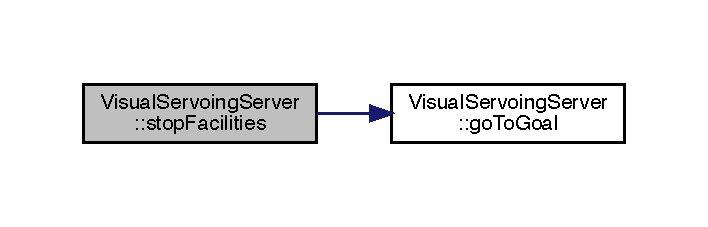
\includegraphics[width=340pt]{classVisualServoingServer_a0cd7a77750df9c1faaf1a18be6305de9_cgraph}
\end{center}
\end{figure}
\mbox{\Hypertarget{classVisualServoingServer_a1c5018056e6a7db492cc6b1418f8d1e5}\label{classVisualServoingServer_a1c5018056e6a7db492cc6b1418f8d1e5}} 
\index{Visual\+Servoing\+Server@{Visual\+Servoing\+Server}!stored\+\_\+go\+\_\+to\+\_\+goal@{stored\+\_\+go\+\_\+to\+\_\+goal}}
\index{stored\+\_\+go\+\_\+to\+\_\+goal@{stored\+\_\+go\+\_\+to\+\_\+goal}!Visual\+Servoing\+Server@{Visual\+Servoing\+Server}}
\subsubsection{\texorpdfstring{stored\+\_\+go\+\_\+to\+\_\+goal()}{stored\_go\_to\_goal()}}
{\footnotesize\ttfamily bool Visual\+Servoing\+Server\+::stored\+\_\+go\+\_\+to\+\_\+goal (\begin{DoxyParamCaption}\item[{const std\+::string \&}]{label }\end{DoxyParamCaption})\hspace{0.3cm}{\ttfamily [override]}, {\ttfamily [protected]}, {\ttfamily [virtual]}}



Set the robot visual servoing goal. 

The goals are stored on an external file and are referenced by a unique label. 
\begin{DoxyParams}{Parameters}
{\em label} & a label referring to one of the available goals; the string shall be one of the available modes returned by the get\+\_\+info() method. \\
\hline
\end{DoxyParams}
\begin{DoxyReturn}{Returns}
true upon success, false otherwise. 
\end{DoxyReturn}


Reimplemented from \hyperlink{classVisualServoingIDL_aa751cf35650259ae7cff331c9d19c694}{Visual\+Servoing\+I\+DL}.



Definition at line 1093 of file Visual\+Servoing\+Server.\+cpp.

\mbox{\Hypertarget{classVisualServoingServer_aded37e0e0111c40fe5f869b16bb1f799}\label{classVisualServoingServer_aded37e0e0111c40fe5f869b16bb1f799}} 
\index{Visual\+Servoing\+Server@{Visual\+Servoing\+Server}!stored\+\_\+init@{stored\+\_\+init}}
\index{stored\+\_\+init@{stored\+\_\+init}!Visual\+Servoing\+Server@{Visual\+Servoing\+Server}}
\subsubsection{\texorpdfstring{stored\+\_\+init()}{stored\_init()}}
{\footnotesize\ttfamily bool Visual\+Servoing\+Server\+::stored\+\_\+init (\begin{DoxyParamCaption}\item[{const std\+::string \&}]{label }\end{DoxyParamCaption})\hspace{0.3cm}{\ttfamily [override]}, {\ttfamily [protected]}, {\ttfamily [virtual]}}



Initialize the robot to an initial position. 

The initial positions are stored on an external file and are referenced by a unique label. 
\begin{DoxyParams}{Parameters}
{\em label} & a label referring to one of the available initial positions; the string shall be one of the available modes returned by the get\+\_\+info() method. \\
\hline
\end{DoxyParams}
\begin{DoxyReturn}{Returns}
true upon success, false otherwise. 
\end{DoxyReturn}


Reimplemented from \hyperlink{classVisualServoingIDL_a20ff1561b87126c9b852eacd5ea59d26}{Visual\+Servoing\+I\+DL}.



Definition at line 1087 of file Visual\+Servoing\+Server.\+cpp.

\mbox{\Hypertarget{classVisualServoingServer_a6d6ec7fee5b76d8a59d75a626b1bd11b}\label{classVisualServoingServer_a6d6ec7fee5b76d8a59d75a626b1bd11b}} 
\index{Visual\+Servoing\+Server@{Visual\+Servoing\+Server}!stored\+Go\+To\+Goal@{stored\+Go\+To\+Goal}}
\index{stored\+Go\+To\+Goal@{stored\+Go\+To\+Goal}!Visual\+Servoing\+Server@{Visual\+Servoing\+Server}}
\subsubsection{\texorpdfstring{stored\+Go\+To\+Goal()}{storedGoToGoal()}}
{\footnotesize\ttfamily bool Visual\+Servoing\+Server\+::stored\+Go\+To\+Goal (\begin{DoxyParamCaption}\item[{const std\+::string \&}]{label }\end{DoxyParamCaption})\hspace{0.3cm}{\ttfamily [override]}}



Definition at line 846 of file Visual\+Servoing\+Server.\+cpp.

\mbox{\Hypertarget{classVisualServoingServer_abf97ec3877e208f4e889a094298a1e1a}\label{classVisualServoingServer_abf97ec3877e208f4e889a094298a1e1a}} 
\index{Visual\+Servoing\+Server@{Visual\+Servoing\+Server}!stored\+Init@{stored\+Init}}
\index{stored\+Init@{stored\+Init}!Visual\+Servoing\+Server@{Visual\+Servoing\+Server}}
\subsubsection{\texorpdfstring{stored\+Init()}{storedInit()}}
{\footnotesize\ttfamily bool Visual\+Servoing\+Server\+::stored\+Init (\begin{DoxyParamCaption}\item[{const std\+::string \&}]{label }\end{DoxyParamCaption})\hspace{0.3cm}{\ttfamily [override]}}



Definition at line 718 of file Visual\+Servoing\+Server.\+cpp.

\mbox{\Hypertarget{classVisualServoingServer_aa8673d3ac18d4aa4be94e8354ef0bad5}\label{classVisualServoingServer_aa8673d3ac18d4aa4be94e8354ef0bad5}} 
\index{Visual\+Servoing\+Server@{Visual\+Servoing\+Server}!thread\+Init@{thread\+Init}}
\index{thread\+Init@{thread\+Init}!Visual\+Servoing\+Server@{Visual\+Servoing\+Server}}
\subsubsection{\texorpdfstring{thread\+Init()}{threadInit()}}
{\footnotesize\ttfamily bool Visual\+Servoing\+Server\+::thread\+Init (\begin{DoxyParamCaption}{ }\end{DoxyParamCaption})\hspace{0.3cm}{\ttfamily [override]}, {\ttfamily [protected]}}



Definition at line 992 of file Visual\+Servoing\+Server.\+cpp.



References backproc\+\_\+\+Update\+Visual\+Servoing\+Paramters().

Here is the call graph for this function\+:
\nopagebreak
\begin{figure}[H]
\begin{center}
\leavevmode
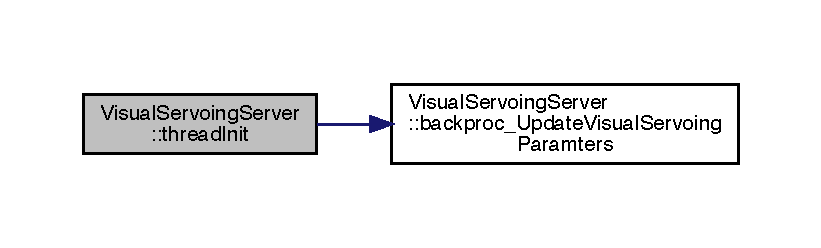
\includegraphics[width=350pt]{classVisualServoingServer_aa8673d3ac18d4aa4be94e8354ef0bad5_cgraph}
\end{center}
\end{figure}
\mbox{\Hypertarget{classVisualServoingServer_a65744a18718c014e19f882dc1052a517}\label{classVisualServoingServer_a65744a18718c014e19f882dc1052a517}} 
\index{Visual\+Servoing\+Server@{Visual\+Servoing\+Server}!thread\+Release@{thread\+Release}}
\index{thread\+Release@{thread\+Release}!Visual\+Servoing\+Server@{Visual\+Servoing\+Server}}
\subsubsection{\texorpdfstring{thread\+Release()}{threadRelease()}}
{\footnotesize\ttfamily void Visual\+Servoing\+Server\+::thread\+Release (\begin{DoxyParamCaption}{ }\end{DoxyParamCaption})\hspace{0.3cm}{\ttfamily [override]}, {\ttfamily [protected]}}



Definition at line 1057 of file Visual\+Servoing\+Server.\+cpp.

\mbox{\Hypertarget{classVisualServoingServer_a509750822f0f1e0db26d54288f8eb1fd}\label{classVisualServoingServer_a509750822f0f1e0db26d54288f8eb1fd}} 
\index{Visual\+Servoing\+Server@{Visual\+Servoing\+Server}!unset\+Torso\+D\+OF@{unset\+Torso\+D\+OF}}
\index{unset\+Torso\+D\+OF@{unset\+Torso\+D\+OF}!Visual\+Servoing\+Server@{Visual\+Servoing\+Server}}
\subsubsection{\texorpdfstring{unset\+Torso\+D\+O\+F()}{unsetTorsoDOF()}}
{\footnotesize\ttfamily bool Visual\+Servoing\+Server\+::unset\+Torso\+D\+OF (\begin{DoxyParamCaption}{ }\end{DoxyParamCaption})\hspace{0.3cm}{\ttfamily [private]}}



Definition at line 2514 of file Visual\+Servoing\+Server.\+cpp.

\mbox{\Hypertarget{classVisualServoingServer_afcd501bb1d5070e8a0735f422a4c9ac0}\label{classVisualServoingServer_afcd501bb1d5070e8a0735f422a4c9ac0}} 
\index{Visual\+Servoing\+Server@{Visual\+Servoing\+Server}!wait\+\_\+visual\+\_\+servoing\+\_\+done@{wait\+\_\+visual\+\_\+servoing\+\_\+done}}
\index{wait\+\_\+visual\+\_\+servoing\+\_\+done@{wait\+\_\+visual\+\_\+servoing\+\_\+done}!Visual\+Servoing\+Server@{Visual\+Servoing\+Server}}
\subsubsection{\texorpdfstring{wait\+\_\+visual\+\_\+servoing\+\_\+done()}{wait\_visual\_servoing\_done()}}
{\footnotesize\ttfamily bool Visual\+Servoing\+Server\+::wait\+\_\+visual\+\_\+servoing\+\_\+done (\begin{DoxyParamCaption}\item[{const double}]{period,  }\item[{const double}]{timeout }\end{DoxyParamCaption})\hspace{0.3cm}{\ttfamily [override]}, {\ttfamily [protected]}, {\ttfamily [virtual]}}



Wait until visual servoing reaches the goal. 

\mbox{[}wait for reply\mbox{]} 
\begin{DoxyParams}{Parameters}
{\em period} & the check time period \mbox{[}s\mbox{]}. \\
\hline
{\em timeout} & the check expiration time \mbox{[}s\mbox{]}. If timeout $<$= 0 (as by default) the check will be performed without time limitation. \\
\hline
\end{DoxyParams}
\begin{DoxyReturn}{Returns}
true for success, false for failure and timeout expired. 
\end{DoxyReturn}
\begin{DoxyNote}{Note}
The tolerance to which the goal is considered achieved can be set with the method \hyperlink{classVisualServoingServer_ad632db85663df2f8c7ca5c27eaacfd71}{set\+Go\+To\+Goal\+Tolerance()}. 

Default values\+: period 0.\+1 \mbox{[}s\mbox{]}, timeout 0.\+0 \mbox{[}s\mbox{]}. 
\end{DoxyNote}


Reimplemented from \hyperlink{classVisualServoingIDL_aa9c9a265e56b0f85c297d2b7d3c8d9c3}{Visual\+Servoing\+I\+DL}.



Definition at line 1226 of file Visual\+Servoing\+Server.\+cpp.

\mbox{\Hypertarget{classVisualServoingServer_a3b462062db0cdcf3c8777469376bb5b6}\label{classVisualServoingServer_a3b462062db0cdcf3c8777469376bb5b6}} 
\index{Visual\+Servoing\+Server@{Visual\+Servoing\+Server}!wait\+Visual\+Servoing\+Done@{wait\+Visual\+Servoing\+Done}}
\index{wait\+Visual\+Servoing\+Done@{wait\+Visual\+Servoing\+Done}!Visual\+Servoing\+Server@{Visual\+Servoing\+Server}}
\subsubsection{\texorpdfstring{wait\+Visual\+Servoing\+Done()}{waitVisualServoingDone()}}
{\footnotesize\ttfamily bool Visual\+Servoing\+Server\+::wait\+Visual\+Servoing\+Done (\begin{DoxyParamCaption}\item[{const double}]{period = {\ttfamily 0.1},  }\item[{const double}]{timeout = {\ttfamily 0.0} }\end{DoxyParamCaption})\hspace{0.3cm}{\ttfamily [override]}}



Definition at line 601 of file Visual\+Servoing\+Server.\+cpp.

\mbox{\Hypertarget{classVisualServoingServer_a8eb3cf6c73a515f6f435f01327d37bd1}\label{classVisualServoingServer_a8eb3cf6c73a515f6f435f01327d37bd1}} 
\index{Visual\+Servoing\+Server@{Visual\+Servoing\+Server}!y\+Error\+Verbose@{y\+Error\+Verbose}}
\index{y\+Error\+Verbose@{y\+Error\+Verbose}!Visual\+Servoing\+Server@{Visual\+Servoing\+Server}}
\subsubsection{\texorpdfstring{y\+Error\+Verbose()}{yErrorVerbose()}}
{\footnotesize\ttfamily void Visual\+Servoing\+Server\+::y\+Error\+Verbose (\begin{DoxyParamCaption}\item[{const yarp\+::os\+::\+Const\+String \&}]{str }\end{DoxyParamCaption}) const\hspace{0.3cm}{\ttfamily [inline]}, {\ttfamily [private]}}



Definition at line 300 of file Visual\+Servoing\+Server.\+h.



References std\+Vector\+Of\+Vectors\+To\+Vector().

Here is the call graph for this function\+:
\nopagebreak
\begin{figure}[H]
\begin{center}
\leavevmode
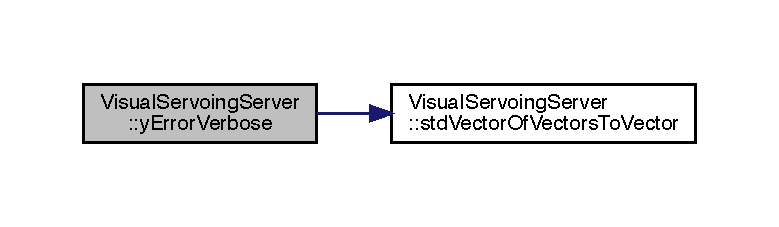
\includegraphics[width=350pt]{classVisualServoingServer_a8eb3cf6c73a515f6f435f01327d37bd1_cgraph}
\end{center}
\end{figure}
\mbox{\Hypertarget{classVisualServoingServer_a6b16f76335ebbd9e4ba9e5ddb67cf883}\label{classVisualServoingServer_a6b16f76335ebbd9e4ba9e5ddb67cf883}} 
\index{Visual\+Servoing\+Server@{Visual\+Servoing\+Server}!y\+Info\+Verbose@{y\+Info\+Verbose}}
\index{y\+Info\+Verbose@{y\+Info\+Verbose}!Visual\+Servoing\+Server@{Visual\+Servoing\+Server}}
\subsubsection{\texorpdfstring{y\+Info\+Verbose()}{yInfoVerbose()}}
{\footnotesize\ttfamily void Visual\+Servoing\+Server\+::y\+Info\+Verbose (\begin{DoxyParamCaption}\item[{const yarp\+::os\+::\+Const\+String \&}]{str }\end{DoxyParamCaption}) const\hspace{0.3cm}{\ttfamily [inline]}, {\ttfamily [private]}}



Definition at line 298 of file Visual\+Servoing\+Server.\+h.

\mbox{\Hypertarget{classVisualServoingServer_a570985820c386689a9507066a016b839}\label{classVisualServoingServer_a570985820c386689a9507066a016b839}} 
\index{Visual\+Servoing\+Server@{Visual\+Servoing\+Server}!y\+Warning\+Verbose@{y\+Warning\+Verbose}}
\index{y\+Warning\+Verbose@{y\+Warning\+Verbose}!Visual\+Servoing\+Server@{Visual\+Servoing\+Server}}
\subsubsection{\texorpdfstring{y\+Warning\+Verbose()}{yWarningVerbose()}}
{\footnotesize\ttfamily void Visual\+Servoing\+Server\+::y\+Warning\+Verbose (\begin{DoxyParamCaption}\item[{const yarp\+::os\+::\+Const\+String \&}]{str }\end{DoxyParamCaption}) const\hspace{0.3cm}{\ttfamily [inline]}, {\ttfamily [private]}}



Definition at line 299 of file Visual\+Servoing\+Server.\+h.



\subsection{Member Data Documentation}
\mbox{\Hypertarget{classVisualServoingServer_a85d6a488bf20eaeb155677a80f731614}\label{classVisualServoingServer_a85d6a488bf20eaeb155677a80f731614}} 
\index{Visual\+Servoing\+Server@{Visual\+Servoing\+Server}!ctx\+\_\+local\+\_\+cart\+\_\+@{ctx\+\_\+local\+\_\+cart\+\_\+}}
\index{ctx\+\_\+local\+\_\+cart\+\_\+@{ctx\+\_\+local\+\_\+cart\+\_\+}!Visual\+Servoing\+Server@{Visual\+Servoing\+Server}}
\subsubsection{\texorpdfstring{ctx\+\_\+local\+\_\+cart\+\_\+}{ctx\_local\_cart\_}}
{\footnotesize\ttfamily int Visual\+Servoing\+Server\+::ctx\+\_\+local\+\_\+cart\+\_\+\hspace{0.3cm}{\ttfamily [private]}}



Definition at line 229 of file Visual\+Servoing\+Server.\+h.

\mbox{\Hypertarget{classVisualServoingServer_a815f9069588f590419cd8645afd3f017}\label{classVisualServoingServer_a815f9069588f590419cd8645afd3f017}} 
\index{Visual\+Servoing\+Server@{Visual\+Servoing\+Server}!ctx\+\_\+remote\+\_\+cart\+\_\+@{ctx\+\_\+remote\+\_\+cart\+\_\+}}
\index{ctx\+\_\+remote\+\_\+cart\+\_\+@{ctx\+\_\+remote\+\_\+cart\+\_\+}!Visual\+Servoing\+Server@{Visual\+Servoing\+Server}}
\subsubsection{\texorpdfstring{ctx\+\_\+remote\+\_\+cart\+\_\+}{ctx\_remote\_cart\_}}
{\footnotesize\ttfamily int Visual\+Servoing\+Server\+::ctx\+\_\+remote\+\_\+cart\+\_\+\hspace{0.3cm}{\ttfamily [private]}}



Definition at line 230 of file Visual\+Servoing\+Server.\+h.

\mbox{\Hypertarget{classVisualServoingServer_a5da42a79826f631e1e40b723e3620c0a}\label{classVisualServoingServer_a5da42a79826f631e1e40b723e3620c0a}} 
\index{Visual\+Servoing\+Server@{Visual\+Servoing\+Server}!gaze\+\_\+driver\+\_\+@{gaze\+\_\+driver\+\_\+}}
\index{gaze\+\_\+driver\+\_\+@{gaze\+\_\+driver\+\_\+}!Visual\+Servoing\+Server@{Visual\+Servoing\+Server}}
\subsubsection{\texorpdfstring{gaze\+\_\+driver\+\_\+}{gaze\_driver\_}}
{\footnotesize\ttfamily yarp\+::dev\+::\+Poly\+Driver Visual\+Servoing\+Server\+::gaze\+\_\+driver\+\_\+\hspace{0.3cm}{\ttfamily [private]}}



Definition at line 187 of file Visual\+Servoing\+Server.\+h.

\mbox{\Hypertarget{classVisualServoingServer_aadfea10f7ca8a2e745c4091d2a1b7c46}\label{classVisualServoingServer_aadfea10f7ca8a2e745c4091d2a1b7c46}} 
\index{Visual\+Servoing\+Server@{Visual\+Servoing\+Server}!goal\+\_\+pose\+\_\+@{goal\+\_\+pose\+\_\+}}
\index{goal\+\_\+pose\+\_\+@{goal\+\_\+pose\+\_\+}!Visual\+Servoing\+Server@{Visual\+Servoing\+Server}}
\subsubsection{\texorpdfstring{goal\+\_\+pose\+\_\+}{goal\_pose\_}}
{\footnotesize\ttfamily yarp\+::sig\+::\+Vector Visual\+Servoing\+Server\+::goal\+\_\+pose\+\_\+ = yarp\+::math\+::zeros(7)\hspace{0.3cm}{\ttfamily [private]}}



Definition at line 214 of file Visual\+Servoing\+Server.\+h.

\mbox{\Hypertarget{classVisualServoingServer_a36243aeb865e36c5e91d3cd3375b9f29}\label{classVisualServoingServer_a36243aeb865e36c5e91d3cd3375b9f29}} 
\index{Visual\+Servoing\+Server@{Visual\+Servoing\+Server}!is\+\_\+stopping\+\_\+backproc\+\_\+update\+\_\+vs\+\_\+params@{is\+\_\+stopping\+\_\+backproc\+\_\+update\+\_\+vs\+\_\+params}}
\index{is\+\_\+stopping\+\_\+backproc\+\_\+update\+\_\+vs\+\_\+params@{is\+\_\+stopping\+\_\+backproc\+\_\+update\+\_\+vs\+\_\+params}!Visual\+Servoing\+Server@{Visual\+Servoing\+Server}}
\subsubsection{\texorpdfstring{is\+\_\+stopping\+\_\+backproc\+\_\+update\+\_\+vs\+\_\+params}{is\_stopping\_backproc\_update\_vs\_params}}
{\footnotesize\ttfamily bool Visual\+Servoing\+Server\+::is\+\_\+stopping\+\_\+backproc\+\_\+update\+\_\+vs\+\_\+params = true\hspace{0.3cm}{\ttfamily [private]}}



Definition at line 288 of file Visual\+Servoing\+Server.\+h.

\mbox{\Hypertarget{classVisualServoingServer_ac884095733af31af336373edbe09eae3}\label{classVisualServoingServer_ac884095733af31af336373edbe09eae3}} 
\index{Visual\+Servoing\+Server@{Visual\+Servoing\+Server}!itf\+\_\+gaze\+\_\+@{itf\+\_\+gaze\+\_\+}}
\index{itf\+\_\+gaze\+\_\+@{itf\+\_\+gaze\+\_\+}!Visual\+Servoing\+Server@{Visual\+Servoing\+Server}}
\subsubsection{\texorpdfstring{itf\+\_\+gaze\+\_\+}{itf\_gaze\_}}
{\footnotesize\ttfamily yarp\+::dev\+::\+I\+Gaze\+Control$\ast$ Visual\+Servoing\+Server\+::itf\+\_\+gaze\+\_\+\hspace{0.3cm}{\ttfamily [private]}}



Definition at line 188 of file Visual\+Servoing\+Server.\+h.

\mbox{\Hypertarget{classVisualServoingServer_a62c8f5c6ba2d62db4754d94984b98632}\label{classVisualServoingServer_a62c8f5c6ba2d62db4754d94984b98632}} 
\index{Visual\+Servoing\+Server@{Visual\+Servoing\+Server}!itf\+\_\+rightarm\+\_\+cart\+\_\+@{itf\+\_\+rightarm\+\_\+cart\+\_\+}}
\index{itf\+\_\+rightarm\+\_\+cart\+\_\+@{itf\+\_\+rightarm\+\_\+cart\+\_\+}!Visual\+Servoing\+Server@{Visual\+Servoing\+Server}}
\subsubsection{\texorpdfstring{itf\+\_\+rightarm\+\_\+cart\+\_\+}{itf\_rightarm\_cart\_}}
{\footnotesize\ttfamily yarp\+::dev\+::\+I\+Cartesian\+Control$\ast$ Visual\+Servoing\+Server\+::itf\+\_\+rightarm\+\_\+cart\+\_\+\hspace{0.3cm}{\ttfamily [private]}}



Definition at line 185 of file Visual\+Servoing\+Server.\+h.

\mbox{\Hypertarget{classVisualServoingServer_a3eaf0fc5ef519ebb94fc89f3a1e490a2}\label{classVisualServoingServer_a3eaf0fc5ef519ebb94fc89f3a1e490a2}} 
\index{Visual\+Servoing\+Server@{Visual\+Servoing\+Server}!K\+\_\+angle\+\_\+tol\+\_\+@{K\+\_\+angle\+\_\+tol\+\_\+}}
\index{K\+\_\+angle\+\_\+tol\+\_\+@{K\+\_\+angle\+\_\+tol\+\_\+}!Visual\+Servoing\+Server@{Visual\+Servoing\+Server}}
\subsubsection{\texorpdfstring{K\+\_\+angle\+\_\+tol\+\_\+}{K\_angle\_tol\_}}
{\footnotesize\ttfamily double Visual\+Servoing\+Server\+::\+K\+\_\+angle\+\_\+tol\+\_\+ = 3.\+0 $\ast$ M\+\_\+\+PI / 180.\+0\hspace{0.3cm}{\ttfamily [private]}}



Definition at line 201 of file Visual\+Servoing\+Server.\+h.

\mbox{\Hypertarget{classVisualServoingServer_a5a7eaa18a77566e129a325e556691e24}\label{classVisualServoingServer_a5a7eaa18a77566e129a325e556691e24}} 
\index{Visual\+Servoing\+Server@{Visual\+Servoing\+Server}!K\+\_\+o\+\_\+@{K\+\_\+o\+\_\+}}
\index{K\+\_\+o\+\_\+@{K\+\_\+o\+\_\+}!Visual\+Servoing\+Server@{Visual\+Servoing\+Server}}
\subsubsection{\texorpdfstring{K\+\_\+o\+\_\+}{K\_o\_}}
{\footnotesize\ttfamily std\+::array$<$double, 2$>$ Visual\+Servoing\+Server\+::\+K\+\_\+o\+\_\+ = \{\{3.\+5, 0.\+5\}\}\hspace{0.3cm}{\ttfamily [private]}}



Definition at line 194 of file Visual\+Servoing\+Server.\+h.

\mbox{\Hypertarget{classVisualServoingServer_a19e92e42912ae3f4d784d80465ed55b1}\label{classVisualServoingServer_a19e92e42912ae3f4d784d80465ed55b1}} 
\index{Visual\+Servoing\+Server@{Visual\+Servoing\+Server}!K\+\_\+o\+\_\+hysteresis\+\_\+@{K\+\_\+o\+\_\+hysteresis\+\_\+}}
\index{K\+\_\+o\+\_\+hysteresis\+\_\+@{K\+\_\+o\+\_\+hysteresis\+\_\+}!Visual\+Servoing\+Server@{Visual\+Servoing\+Server}}
\subsubsection{\texorpdfstring{K\+\_\+o\+\_\+hysteresis\+\_\+}{K\_o\_hysteresis\_}}
{\footnotesize\ttfamily bool Visual\+Servoing\+Server\+::\+K\+\_\+o\+\_\+hysteresis\+\_\+ = false\hspace{0.3cm}{\ttfamily [private]}}



Definition at line 203 of file Visual\+Servoing\+Server.\+h.

\mbox{\Hypertarget{classVisualServoingServer_ab372aee55fa6ffb7d87d0f9103ea3266}\label{classVisualServoingServer_ab372aee55fa6ffb7d87d0f9103ea3266}} 
\index{Visual\+Servoing\+Server@{Visual\+Servoing\+Server}!K\+\_\+o\+\_\+tol\+\_\+@{K\+\_\+o\+\_\+tol\+\_\+}}
\index{K\+\_\+o\+\_\+tol\+\_\+@{K\+\_\+o\+\_\+tol\+\_\+}!Visual\+Servoing\+Server@{Visual\+Servoing\+Server}}
\subsubsection{\texorpdfstring{K\+\_\+o\+\_\+tol\+\_\+}{K\_o\_tol\_}}
{\footnotesize\ttfamily double Visual\+Servoing\+Server\+::\+K\+\_\+o\+\_\+tol\+\_\+ = 10.\+0\hspace{0.3cm}{\ttfamily [private]}}



Definition at line 198 of file Visual\+Servoing\+Server.\+h.

\mbox{\Hypertarget{classVisualServoingServer_ab1c7e6dbab2608694d520e849da043f8}\label{classVisualServoingServer_ab1c7e6dbab2608694d520e849da043f8}} 
\index{Visual\+Servoing\+Server@{Visual\+Servoing\+Server}!K\+\_\+orientation\+\_\+tol\+\_\+@{K\+\_\+orientation\+\_\+tol\+\_\+}}
\index{K\+\_\+orientation\+\_\+tol\+\_\+@{K\+\_\+orientation\+\_\+tol\+\_\+}!Visual\+Servoing\+Server@{Visual\+Servoing\+Server}}
\subsubsection{\texorpdfstring{K\+\_\+orientation\+\_\+tol\+\_\+}{K\_orientation\_tol\_}}
{\footnotesize\ttfamily double Visual\+Servoing\+Server\+::\+K\+\_\+orientation\+\_\+tol\+\_\+ = 9.\+0 $\ast$ M\+\_\+\+PI / 180.\+0\hspace{0.3cm}{\ttfamily [private]}}



Definition at line 200 of file Visual\+Servoing\+Server.\+h.

\mbox{\Hypertarget{classVisualServoingServer_a4fdd46d1c8be0e8eb8b28af84cfe8a6b}\label{classVisualServoingServer_a4fdd46d1c8be0e8eb8b28af84cfe8a6b}} 
\index{Visual\+Servoing\+Server@{Visual\+Servoing\+Server}!K\+\_\+pose\+\_\+hysteresis\+\_\+@{K\+\_\+pose\+\_\+hysteresis\+\_\+}}
\index{K\+\_\+pose\+\_\+hysteresis\+\_\+@{K\+\_\+pose\+\_\+hysteresis\+\_\+}!Visual\+Servoing\+Server@{Visual\+Servoing\+Server}}
\subsubsection{\texorpdfstring{K\+\_\+pose\+\_\+hysteresis\+\_\+}{K\_pose\_hysteresis\_}}
{\footnotesize\ttfamily bool Visual\+Servoing\+Server\+::\+K\+\_\+pose\+\_\+hysteresis\+\_\+ = false\hspace{0.3cm}{\ttfamily [private]}}



Definition at line 204 of file Visual\+Servoing\+Server.\+h.

\mbox{\Hypertarget{classVisualServoingServer_aaef2ff3c3853c7a73bc620225f824e4e}\label{classVisualServoingServer_aaef2ff3c3853c7a73bc620225f824e4e}} 
\index{Visual\+Servoing\+Server@{Visual\+Servoing\+Server}!K\+\_\+position\+\_\+tol\+\_\+@{K\+\_\+position\+\_\+tol\+\_\+}}
\index{K\+\_\+position\+\_\+tol\+\_\+@{K\+\_\+position\+\_\+tol\+\_\+}!Visual\+Servoing\+Server@{Visual\+Servoing\+Server}}
\subsubsection{\texorpdfstring{K\+\_\+position\+\_\+tol\+\_\+}{K\_position\_tol\_}}
{\footnotesize\ttfamily double Visual\+Servoing\+Server\+::\+K\+\_\+position\+\_\+tol\+\_\+ = 0.\+03\hspace{0.3cm}{\ttfamily [private]}}



Definition at line 199 of file Visual\+Servoing\+Server.\+h.

\mbox{\Hypertarget{classVisualServoingServer_a6153b1e315817cf41cb36b7deca83be7}\label{classVisualServoingServer_a6153b1e315817cf41cb36b7deca83be7}} 
\index{Visual\+Servoing\+Server@{Visual\+Servoing\+Server}!K\+\_\+x\+\_\+@{K\+\_\+x\+\_\+}}
\index{K\+\_\+x\+\_\+@{K\+\_\+x\+\_\+}!Visual\+Servoing\+Server@{Visual\+Servoing\+Server}}
\subsubsection{\texorpdfstring{K\+\_\+x\+\_\+}{K\_x\_}}
{\footnotesize\ttfamily std\+::array$<$double, 2$>$ Visual\+Servoing\+Server\+::\+K\+\_\+x\+\_\+ = \{\{0.\+5, 0.\+25\}\}\hspace{0.3cm}{\ttfamily [private]}}



Definition at line 193 of file Visual\+Servoing\+Server.\+h.

\mbox{\Hypertarget{classVisualServoingServer_a8b8f0cda1bb882c1783db88b720b5597}\label{classVisualServoingServer_a8b8f0cda1bb882c1783db88b720b5597}} 
\index{Visual\+Servoing\+Server@{Visual\+Servoing\+Server}!K\+\_\+x\+\_\+hysteresis\+\_\+@{K\+\_\+x\+\_\+hysteresis\+\_\+}}
\index{K\+\_\+x\+\_\+hysteresis\+\_\+@{K\+\_\+x\+\_\+hysteresis\+\_\+}!Visual\+Servoing\+Server@{Visual\+Servoing\+Server}}
\subsubsection{\texorpdfstring{K\+\_\+x\+\_\+hysteresis\+\_\+}{K\_x\_hysteresis\_}}
{\footnotesize\ttfamily bool Visual\+Servoing\+Server\+::\+K\+\_\+x\+\_\+hysteresis\+\_\+ = false\hspace{0.3cm}{\ttfamily [private]}}



Definition at line 202 of file Visual\+Servoing\+Server.\+h.

\mbox{\Hypertarget{classVisualServoingServer_aa59bfed390207a42a4a05dd1fe720f6b}\label{classVisualServoingServer_aa59bfed390207a42a4a05dd1fe720f6b}} 
\index{Visual\+Servoing\+Server@{Visual\+Servoing\+Server}!K\+\_\+x\+\_\+tol\+\_\+@{K\+\_\+x\+\_\+tol\+\_\+}}
\index{K\+\_\+x\+\_\+tol\+\_\+@{K\+\_\+x\+\_\+tol\+\_\+}!Visual\+Servoing\+Server@{Visual\+Servoing\+Server}}
\subsubsection{\texorpdfstring{K\+\_\+x\+\_\+tol\+\_\+}{K\_x\_tol\_}}
{\footnotesize\ttfamily double Visual\+Servoing\+Server\+::\+K\+\_\+x\+\_\+tol\+\_\+ = 10.\+0\hspace{0.3cm}{\ttfamily [private]}}



Definition at line 197 of file Visual\+Servoing\+Server.\+h.

\mbox{\Hypertarget{classVisualServoingServer_afbf7be0f4c935dcbcd8a23b07b7972ba}\label{classVisualServoingServer_afbf7be0f4c935dcbcd8a23b07b7972ba}} 
\index{Visual\+Servoing\+Server@{Visual\+Servoing\+Server}!l\+\_\+\+H\+\_\+eye\+\_\+to\+\_\+r\+\_\+@{l\+\_\+\+H\+\_\+eye\+\_\+to\+\_\+r\+\_\+}}
\index{l\+\_\+\+H\+\_\+eye\+\_\+to\+\_\+r\+\_\+@{l\+\_\+\+H\+\_\+eye\+\_\+to\+\_\+r\+\_\+}!Visual\+Servoing\+Server@{Visual\+Servoing\+Server}}
\subsubsection{\texorpdfstring{l\+\_\+\+H\+\_\+eye\+\_\+to\+\_\+r\+\_\+}{l\_H\_eye\_to\_r\_}}
{\footnotesize\ttfamily yarp\+::sig\+::\+Matrix Visual\+Servoing\+Server\+::l\+\_\+\+H\+\_\+eye\+\_\+to\+\_\+r\+\_\+ = yarp\+::math\+::zeros(4, 4)\hspace{0.3cm}{\ttfamily [private]}}



Definition at line 216 of file Visual\+Servoing\+Server.\+h.

\mbox{\Hypertarget{classVisualServoingServer_a43b53260b0903efb5479becf664f33ae}\label{classVisualServoingServer_a43b53260b0903efb5479becf664f33ae}} 
\index{Visual\+Servoing\+Server@{Visual\+Servoing\+Server}!l\+\_\+\+H\+\_\+r\+\_\+to\+\_\+cam\+\_\+@{l\+\_\+\+H\+\_\+r\+\_\+to\+\_\+cam\+\_\+}}
\index{l\+\_\+\+H\+\_\+r\+\_\+to\+\_\+cam\+\_\+@{l\+\_\+\+H\+\_\+r\+\_\+to\+\_\+cam\+\_\+}!Visual\+Servoing\+Server@{Visual\+Servoing\+Server}}
\subsubsection{\texorpdfstring{l\+\_\+\+H\+\_\+r\+\_\+to\+\_\+cam\+\_\+}{l\_H\_r\_to\_cam\_}}
{\footnotesize\ttfamily yarp\+::sig\+::\+Matrix Visual\+Servoing\+Server\+::l\+\_\+\+H\+\_\+r\+\_\+to\+\_\+cam\+\_\+ = yarp\+::math\+::zeros(4, 4)\hspace{0.3cm}{\ttfamily [private]}}



Definition at line 218 of file Visual\+Servoing\+Server.\+h.

\mbox{\Hypertarget{classVisualServoingServer_a19525066e8d98f781f28600ff526ce68}\label{classVisualServoingServer_a19525066e8d98f781f28600ff526ce68}} 
\index{Visual\+Servoing\+Server@{Visual\+Servoing\+Server}!l\+\_\+proj\+\_\+@{l\+\_\+proj\+\_\+}}
\index{l\+\_\+proj\+\_\+@{l\+\_\+proj\+\_\+}!Visual\+Servoing\+Server@{Visual\+Servoing\+Server}}
\subsubsection{\texorpdfstring{l\+\_\+proj\+\_\+}{l\_proj\_}}
{\footnotesize\ttfamily yarp\+::sig\+::\+Matrix Visual\+Servoing\+Server\+::l\+\_\+proj\+\_\+\hspace{0.3cm}{\ttfamily [private]}}



Definition at line 211 of file Visual\+Servoing\+Server.\+h.

\mbox{\Hypertarget{classVisualServoingServer_a3f7efc9e5a4bbb030a4dd81030643398}\label{classVisualServoingServer_a3f7efc9e5a4bbb030a4dd81030643398}} 
\index{Visual\+Servoing\+Server@{Visual\+Servoing\+Server}!l\+\_\+px\+\_\+goal\+\_\+@{l\+\_\+px\+\_\+goal\+\_\+}}
\index{l\+\_\+px\+\_\+goal\+\_\+@{l\+\_\+px\+\_\+goal\+\_\+}!Visual\+Servoing\+Server@{Visual\+Servoing\+Server}}
\subsubsection{\texorpdfstring{l\+\_\+px\+\_\+goal\+\_\+}{l\_px\_goal\_}}
{\footnotesize\ttfamily std\+::vector$<$yarp\+::sig\+::\+Vector$>$ Visual\+Servoing\+Server\+::l\+\_\+px\+\_\+goal\+\_\+ = std\+::vector$<$yarp\+::sig\+::\+Vector$>$(4)\hspace{0.3cm}{\ttfamily [private]}}



Definition at line 226 of file Visual\+Servoing\+Server.\+h.

\mbox{\Hypertarget{classVisualServoingServer_a2fb091edd86b425b79b36c968a0929e1}\label{classVisualServoingServer_a2fb091edd86b425b79b36c968a0929e1}} 
\index{Visual\+Servoing\+Server@{Visual\+Servoing\+Server}!max\+\_\+o\+\_\+dot\+\_\+@{max\+\_\+o\+\_\+dot\+\_\+}}
\index{max\+\_\+o\+\_\+dot\+\_\+@{max\+\_\+o\+\_\+dot\+\_\+}!Visual\+Servoing\+Server@{Visual\+Servoing\+Server}}
\subsubsection{\texorpdfstring{max\+\_\+o\+\_\+dot\+\_\+}{max\_o\_dot\_}}
{\footnotesize\ttfamily double Visual\+Servoing\+Server\+::max\+\_\+o\+\_\+dot\+\_\+ = 10.\+0 $\ast$ M\+\_\+\+PI / 180.\+0\hspace{0.3cm}{\ttfamily [private]}}



Definition at line 196 of file Visual\+Servoing\+Server.\+h.

\mbox{\Hypertarget{classVisualServoingServer_a82df6acf27455af727ce31758856ee48}\label{classVisualServoingServer_a82df6acf27455af727ce31758856ee48}} 
\index{Visual\+Servoing\+Server@{Visual\+Servoing\+Server}!max\+\_\+x\+\_\+dot\+\_\+@{max\+\_\+x\+\_\+dot\+\_\+}}
\index{max\+\_\+x\+\_\+dot\+\_\+@{max\+\_\+x\+\_\+dot\+\_\+}!Visual\+Servoing\+Server@{Visual\+Servoing\+Server}}
\subsubsection{\texorpdfstring{max\+\_\+x\+\_\+dot\+\_\+}{max\_x\_dot\_}}
{\footnotesize\ttfamily double Visual\+Servoing\+Server\+::max\+\_\+x\+\_\+dot\+\_\+ = 0.\+035\hspace{0.3cm}{\ttfamily [private]}}



Definition at line 195 of file Visual\+Servoing\+Server.\+h.

\mbox{\Hypertarget{classVisualServoingServer_a379f8205d854495f481bbaa37825dfcb}\label{classVisualServoingServer_a379f8205d854495f481bbaa37825dfcb}} 
\index{Visual\+Servoing\+Server@{Visual\+Servoing\+Server}!mtx\+\_\+\+H\+\_\+eye\+\_\+cam\+\_\+@{mtx\+\_\+\+H\+\_\+eye\+\_\+cam\+\_\+}}
\index{mtx\+\_\+\+H\+\_\+eye\+\_\+cam\+\_\+@{mtx\+\_\+\+H\+\_\+eye\+\_\+cam\+\_\+}!Visual\+Servoing\+Server@{Visual\+Servoing\+Server}}
\subsubsection{\texorpdfstring{mtx\+\_\+\+H\+\_\+eye\+\_\+cam\+\_\+}{mtx\_H\_eye\_cam\_}}
{\footnotesize\ttfamily std\+::mutex Visual\+Servoing\+Server\+::mtx\+\_\+\+H\+\_\+eye\+\_\+cam\+\_\+\hspace{0.3cm}{\ttfamily [private]}}



Definition at line 222 of file Visual\+Servoing\+Server.\+h.

\mbox{\Hypertarget{classVisualServoingServer_a63758b38bb0069515d047449aafc9597}\label{classVisualServoingServer_a63758b38bb0069515d047449aafc9597}} 
\index{Visual\+Servoing\+Server@{Visual\+Servoing\+Server}!mtx\+\_\+px\+\_\+des\+\_\+@{mtx\+\_\+px\+\_\+des\+\_\+}}
\index{mtx\+\_\+px\+\_\+des\+\_\+@{mtx\+\_\+px\+\_\+des\+\_\+}!Visual\+Servoing\+Server@{Visual\+Servoing\+Server}}
\subsubsection{\texorpdfstring{mtx\+\_\+px\+\_\+des\+\_\+}{mtx\_px\_des\_}}
{\footnotesize\ttfamily std\+::mutex Visual\+Servoing\+Server\+::mtx\+\_\+px\+\_\+des\+\_\+\hspace{0.3cm}{\ttfamily [private]}}



Definition at line 221 of file Visual\+Servoing\+Server.\+h.

\mbox{\Hypertarget{classVisualServoingServer_af6b808cf1ef56df5fb432196335e1ceb}\label{classVisualServoingServer_af6b808cf1ef56df5fb432196335e1ceb}} 
\index{Visual\+Servoing\+Server@{Visual\+Servoing\+Server}!op\+\_\+mode\+\_\+@{op\+\_\+mode\+\_\+}}
\index{op\+\_\+mode\+\_\+@{op\+\_\+mode\+\_\+}!Visual\+Servoing\+Server@{Visual\+Servoing\+Server}}
\subsubsection{\texorpdfstring{op\+\_\+mode\+\_\+}{op\_mode\_}}
{\footnotesize\ttfamily \hyperlink{classVisualServoingServer_ab4ac95327e1829713374ca3cd0dec915}{Operating\+Mode} Visual\+Servoing\+Server\+::op\+\_\+mode\+\_\+ = \hyperlink{classVisualServoingServer_ab4ac95327e1829713374ca3cd0dec915a2d5f8ae9328c6535be72ed28bff47560}{Operating\+Mode\+::pose}\hspace{0.3cm}{\ttfamily [private]}}



Definition at line 182 of file Visual\+Servoing\+Server.\+h.

\mbox{\Hypertarget{classVisualServoingServer_a46d59d98a68e0a88b810835c447241f6}\label{classVisualServoingServer_a46d59d98a68e0a88b810835c447241f6}} 
\index{Visual\+Servoing\+Server@{Visual\+Servoing\+Server}!port\+\_\+click\+\_\+left\+\_\+@{port\+\_\+click\+\_\+left\+\_\+}}
\index{port\+\_\+click\+\_\+left\+\_\+@{port\+\_\+click\+\_\+left\+\_\+}!Visual\+Servoing\+Server@{Visual\+Servoing\+Server}}
\subsubsection{\texorpdfstring{port\+\_\+click\+\_\+left\+\_\+}{port\_click\_left\_}}
{\footnotesize\ttfamily yarp\+::os\+::\+Buffered\+Port$<$yarp\+::os\+::\+Bottle$>$ Visual\+Servoing\+Server\+::port\+\_\+click\+\_\+left\+\_\+\hspace{0.3cm}{\ttfamily [private]}}



Definition at line 237 of file Visual\+Servoing\+Server.\+h.

\mbox{\Hypertarget{classVisualServoingServer_a67701a55fce8ed1301417ecda99eff06}\label{classVisualServoingServer_a67701a55fce8ed1301417ecda99eff06}} 
\index{Visual\+Servoing\+Server@{Visual\+Servoing\+Server}!port\+\_\+click\+\_\+right\+\_\+@{port\+\_\+click\+\_\+right\+\_\+}}
\index{port\+\_\+click\+\_\+right\+\_\+@{port\+\_\+click\+\_\+right\+\_\+}!Visual\+Servoing\+Server@{Visual\+Servoing\+Server}}
\subsubsection{\texorpdfstring{port\+\_\+click\+\_\+right\+\_\+}{port\_click\_right\_}}
{\footnotesize\ttfamily yarp\+::os\+::\+Buffered\+Port$<$yarp\+::os\+::\+Bottle$>$ Visual\+Servoing\+Server\+::port\+\_\+click\+\_\+right\+\_\+\hspace{0.3cm}{\ttfamily [private]}}



Definition at line 241 of file Visual\+Servoing\+Server.\+h.

\mbox{\Hypertarget{classVisualServoingServer_ac4fad3f3691ad57d8a1f693e573f75be}\label{classVisualServoingServer_ac4fad3f3691ad57d8a1f693e573f75be}} 
\index{Visual\+Servoing\+Server@{Visual\+Servoing\+Server}!port\+\_\+goal\+\_\+px\+\_\+l\+\_\+@{port\+\_\+goal\+\_\+px\+\_\+l\+\_\+}}
\index{port\+\_\+goal\+\_\+px\+\_\+l\+\_\+@{port\+\_\+goal\+\_\+px\+\_\+l\+\_\+}!Visual\+Servoing\+Server@{Visual\+Servoing\+Server}}
\subsubsection{\texorpdfstring{port\+\_\+goal\+\_\+px\+\_\+l\+\_\+}{port\_goal\_px\_l\_}}
{\footnotesize\ttfamily yarp\+::os\+::\+Buffered\+Port$<$yarp\+::sig\+::\+Vector$>$ Visual\+Servoing\+Server\+::port\+\_\+goal\+\_\+px\+\_\+l\+\_\+\hspace{0.3cm}{\ttfamily [private]}}



Definition at line 310 of file Visual\+Servoing\+Server.\+h.

\mbox{\Hypertarget{classVisualServoingServer_ad06d05e912dbba4c1ded31ae6e0e3004}\label{classVisualServoingServer_ad06d05e912dbba4c1ded31ae6e0e3004}} 
\index{Visual\+Servoing\+Server@{Visual\+Servoing\+Server}!port\+\_\+goal\+\_\+px\+\_\+r\+\_\+@{port\+\_\+goal\+\_\+px\+\_\+r\+\_\+}}
\index{port\+\_\+goal\+\_\+px\+\_\+r\+\_\+@{port\+\_\+goal\+\_\+px\+\_\+r\+\_\+}!Visual\+Servoing\+Server@{Visual\+Servoing\+Server}}
\subsubsection{\texorpdfstring{port\+\_\+goal\+\_\+px\+\_\+r\+\_\+}{port\_goal\_px\_r\_}}
{\footnotesize\ttfamily yarp\+::os\+::\+Buffered\+Port$<$yarp\+::sig\+::\+Vector$>$ Visual\+Servoing\+Server\+::port\+\_\+goal\+\_\+px\+\_\+r\+\_\+\hspace{0.3cm}{\ttfamily [private]}}



Definition at line 311 of file Visual\+Servoing\+Server.\+h.

\mbox{\Hypertarget{classVisualServoingServer_a0561904e7a2d8f680812f042eec3b2d8}\label{classVisualServoingServer_a0561904e7a2d8f680812f042eec3b2d8}} 
\index{Visual\+Servoing\+Server@{Visual\+Servoing\+Server}!port\+\_\+image\+\_\+left\+\_\+in\+\_\+@{port\+\_\+image\+\_\+left\+\_\+in\+\_\+}}
\index{port\+\_\+image\+\_\+left\+\_\+in\+\_\+@{port\+\_\+image\+\_\+left\+\_\+in\+\_\+}!Visual\+Servoing\+Server@{Visual\+Servoing\+Server}}
\subsubsection{\texorpdfstring{port\+\_\+image\+\_\+left\+\_\+in\+\_\+}{port\_image\_left\_in\_}}
{\footnotesize\ttfamily yarp\+::os\+::\+Buffered\+Port$<$yarp\+::sig\+::\+Image\+Of$<$yarp\+::sig\+::\+Pixel\+Rgb$>$ $>$ Visual\+Servoing\+Server\+::port\+\_\+image\+\_\+left\+\_\+in\+\_\+\hspace{0.3cm}{\ttfamily [private]}}



Definition at line 235 of file Visual\+Servoing\+Server.\+h.

\mbox{\Hypertarget{classVisualServoingServer_ac8e9e8c8e3c0a412bd1dd464b58931bd}\label{classVisualServoingServer_ac8e9e8c8e3c0a412bd1dd464b58931bd}} 
\index{Visual\+Servoing\+Server@{Visual\+Servoing\+Server}!port\+\_\+image\+\_\+left\+\_\+out\+\_\+@{port\+\_\+image\+\_\+left\+\_\+out\+\_\+}}
\index{port\+\_\+image\+\_\+left\+\_\+out\+\_\+@{port\+\_\+image\+\_\+left\+\_\+out\+\_\+}!Visual\+Servoing\+Server@{Visual\+Servoing\+Server}}
\subsubsection{\texorpdfstring{port\+\_\+image\+\_\+left\+\_\+out\+\_\+}{port\_image\_left\_out\_}}
{\footnotesize\ttfamily yarp\+::os\+::\+Buffered\+Port$<$yarp\+::sig\+::\+Image\+Of$<$yarp\+::sig\+::\+Pixel\+Rgb$>$ $>$ Visual\+Servoing\+Server\+::port\+\_\+image\+\_\+left\+\_\+out\+\_\+\hspace{0.3cm}{\ttfamily [private]}}



Definition at line 236 of file Visual\+Servoing\+Server.\+h.

\mbox{\Hypertarget{classVisualServoingServer_a776855ca4deb47cf1c739bde2e07bc8e}\label{classVisualServoingServer_a776855ca4deb47cf1c739bde2e07bc8e}} 
\index{Visual\+Servoing\+Server@{Visual\+Servoing\+Server}!port\+\_\+image\+\_\+right\+\_\+in\+\_\+@{port\+\_\+image\+\_\+right\+\_\+in\+\_\+}}
\index{port\+\_\+image\+\_\+right\+\_\+in\+\_\+@{port\+\_\+image\+\_\+right\+\_\+in\+\_\+}!Visual\+Servoing\+Server@{Visual\+Servoing\+Server}}
\subsubsection{\texorpdfstring{port\+\_\+image\+\_\+right\+\_\+in\+\_\+}{port\_image\_right\_in\_}}
{\footnotesize\ttfamily yarp\+::os\+::\+Buffered\+Port$<$yarp\+::sig\+::\+Image\+Of$<$yarp\+::sig\+::\+Pixel\+Rgb$>$ $>$ Visual\+Servoing\+Server\+::port\+\_\+image\+\_\+right\+\_\+in\+\_\+\hspace{0.3cm}{\ttfamily [private]}}



Definition at line 239 of file Visual\+Servoing\+Server.\+h.

\mbox{\Hypertarget{classVisualServoingServer_ab5c7a20d3e8545331970517c75d79f2a}\label{classVisualServoingServer_ab5c7a20d3e8545331970517c75d79f2a}} 
\index{Visual\+Servoing\+Server@{Visual\+Servoing\+Server}!port\+\_\+image\+\_\+right\+\_\+out\+\_\+@{port\+\_\+image\+\_\+right\+\_\+out\+\_\+}}
\index{port\+\_\+image\+\_\+right\+\_\+out\+\_\+@{port\+\_\+image\+\_\+right\+\_\+out\+\_\+}!Visual\+Servoing\+Server@{Visual\+Servoing\+Server}}
\subsubsection{\texorpdfstring{port\+\_\+image\+\_\+right\+\_\+out\+\_\+}{port\_image\_right\_out\_}}
{\footnotesize\ttfamily yarp\+::os\+::\+Buffered\+Port$<$yarp\+::sig\+::\+Image\+Of$<$yarp\+::sig\+::\+Pixel\+Rgb$>$ $>$ Visual\+Servoing\+Server\+::port\+\_\+image\+\_\+right\+\_\+out\+\_\+\hspace{0.3cm}{\ttfamily [private]}}



Definition at line 240 of file Visual\+Servoing\+Server.\+h.

\mbox{\Hypertarget{classVisualServoingServer_a5c6969762a136abeb5de050637e6fbc7}\label{classVisualServoingServer_a5c6969762a136abeb5de050637e6fbc7}} 
\index{Visual\+Servoing\+Server@{Visual\+Servoing\+Server}!port\+\_\+kin\+\_\+px\+\_\+l\+\_\+@{port\+\_\+kin\+\_\+px\+\_\+l\+\_\+}}
\index{port\+\_\+kin\+\_\+px\+\_\+l\+\_\+@{port\+\_\+kin\+\_\+px\+\_\+l\+\_\+}!Visual\+Servoing\+Server@{Visual\+Servoing\+Server}}
\subsubsection{\texorpdfstring{port\+\_\+kin\+\_\+px\+\_\+l\+\_\+}{port\_kin\_px\_l\_}}
{\footnotesize\ttfamily yarp\+::os\+::\+Buffered\+Port$<$yarp\+::sig\+::\+Vector$>$ Visual\+Servoing\+Server\+::port\+\_\+kin\+\_\+px\+\_\+l\+\_\+\hspace{0.3cm}{\ttfamily [private]}}



Definition at line 307 of file Visual\+Servoing\+Server.\+h.

\mbox{\Hypertarget{classVisualServoingServer_a0a681791d720678229a3365a5bb0bfd6}\label{classVisualServoingServer_a0a681791d720678229a3365a5bb0bfd6}} 
\index{Visual\+Servoing\+Server@{Visual\+Servoing\+Server}!port\+\_\+kin\+\_\+px\+\_\+r\+\_\+@{port\+\_\+kin\+\_\+px\+\_\+r\+\_\+}}
\index{port\+\_\+kin\+\_\+px\+\_\+r\+\_\+@{port\+\_\+kin\+\_\+px\+\_\+r\+\_\+}!Visual\+Servoing\+Server@{Visual\+Servoing\+Server}}
\subsubsection{\texorpdfstring{port\+\_\+kin\+\_\+px\+\_\+r\+\_\+}{port\_kin\_px\_r\_}}
{\footnotesize\ttfamily yarp\+::os\+::\+Buffered\+Port$<$yarp\+::sig\+::\+Vector$>$ Visual\+Servoing\+Server\+::port\+\_\+kin\+\_\+px\+\_\+r\+\_\+\hspace{0.3cm}{\ttfamily [private]}}



Definition at line 308 of file Visual\+Servoing\+Server.\+h.

\mbox{\Hypertarget{classVisualServoingServer_a31db93e3ee0db64e8681d762428b85a9}\label{classVisualServoingServer_a31db93e3ee0db64e8681d762428b85a9}} 
\index{Visual\+Servoing\+Server@{Visual\+Servoing\+Server}!port\+\_\+pose\+\_\+avg\+\_\+@{port\+\_\+pose\+\_\+avg\+\_\+}}
\index{port\+\_\+pose\+\_\+avg\+\_\+@{port\+\_\+pose\+\_\+avg\+\_\+}!Visual\+Servoing\+Server@{Visual\+Servoing\+Server}}
\subsubsection{\texorpdfstring{port\+\_\+pose\+\_\+avg\+\_\+}{port\_pose\_avg\_}}
{\footnotesize\ttfamily yarp\+::os\+::\+Buffered\+Port$<$yarp\+::sig\+::\+Vector$>$ Visual\+Servoing\+Server\+::port\+\_\+pose\+\_\+avg\+\_\+\hspace{0.3cm}{\ttfamily [private]}}



Definition at line 313 of file Visual\+Servoing\+Server.\+h.

\mbox{\Hypertarget{classVisualServoingServer_a73e57c16019ed76e14e92a600f1e761b}\label{classVisualServoingServer_a73e57c16019ed76e14e92a600f1e761b}} 
\index{Visual\+Servoing\+Server@{Visual\+Servoing\+Server}!port\+\_\+pose\+\_\+goal\+\_\+@{port\+\_\+pose\+\_\+goal\+\_\+}}
\index{port\+\_\+pose\+\_\+goal\+\_\+@{port\+\_\+pose\+\_\+goal\+\_\+}!Visual\+Servoing\+Server@{Visual\+Servoing\+Server}}
\subsubsection{\texorpdfstring{port\+\_\+pose\+\_\+goal\+\_\+}{port\_pose\_goal\_}}
{\footnotesize\ttfamily yarp\+::os\+::\+Buffered\+Port$<$yarp\+::sig\+::\+Vector$>$ Visual\+Servoing\+Server\+::port\+\_\+pose\+\_\+goal\+\_\+\hspace{0.3cm}{\ttfamily [private]}}



Definition at line 315 of file Visual\+Servoing\+Server.\+h.

\mbox{\Hypertarget{classVisualServoingServer_a0f4787672f7b6dea128d688aff2056fc}\label{classVisualServoingServer_a0f4787672f7b6dea128d688aff2056fc}} 
\index{Visual\+Servoing\+Server@{Visual\+Servoing\+Server}!port\+\_\+pose\+\_\+kin\+\_\+@{port\+\_\+pose\+\_\+kin\+\_\+}}
\index{port\+\_\+pose\+\_\+kin\+\_\+@{port\+\_\+pose\+\_\+kin\+\_\+}!Visual\+Servoing\+Server@{Visual\+Servoing\+Server}}
\subsubsection{\texorpdfstring{port\+\_\+pose\+\_\+kin\+\_\+}{port\_pose\_kin\_}}
{\footnotesize\ttfamily yarp\+::os\+::\+Buffered\+Port$<$yarp\+::sig\+::\+Vector$>$ Visual\+Servoing\+Server\+::port\+\_\+pose\+\_\+kin\+\_\+\hspace{0.3cm}{\ttfamily [private]}}



Definition at line 314 of file Visual\+Servoing\+Server.\+h.

\mbox{\Hypertarget{classVisualServoingServer_a4c250786d095b0e8a8f5546b2976a669}\label{classVisualServoingServer_a4c250786d095b0e8a8f5546b2976a669}} 
\index{Visual\+Servoing\+Server@{Visual\+Servoing\+Server}!port\+\_\+pose\+\_\+left\+\_\+in\+\_\+@{port\+\_\+pose\+\_\+left\+\_\+in\+\_\+}}
\index{port\+\_\+pose\+\_\+left\+\_\+in\+\_\+@{port\+\_\+pose\+\_\+left\+\_\+in\+\_\+}!Visual\+Servoing\+Server@{Visual\+Servoing\+Server}}
\subsubsection{\texorpdfstring{port\+\_\+pose\+\_\+left\+\_\+in\+\_\+}{port\_pose\_left\_in\_}}
{\footnotesize\ttfamily yarp\+::os\+::\+Buffered\+Port$<$yarp\+::sig\+::\+Vector$>$ Visual\+Servoing\+Server\+::port\+\_\+pose\+\_\+left\+\_\+in\+\_\+\hspace{0.3cm}{\ttfamily [private]}}



Definition at line 232 of file Visual\+Servoing\+Server.\+h.

\mbox{\Hypertarget{classVisualServoingServer_aa72393af28f4b424eeb2966962cbd319}\label{classVisualServoingServer_aa72393af28f4b424eeb2966962cbd319}} 
\index{Visual\+Servoing\+Server@{Visual\+Servoing\+Server}!port\+\_\+pose\+\_\+px\+\_\+l\+\_\+@{port\+\_\+pose\+\_\+px\+\_\+l\+\_\+}}
\index{port\+\_\+pose\+\_\+px\+\_\+l\+\_\+@{port\+\_\+pose\+\_\+px\+\_\+l\+\_\+}!Visual\+Servoing\+Server@{Visual\+Servoing\+Server}}
\subsubsection{\texorpdfstring{port\+\_\+pose\+\_\+px\+\_\+l\+\_\+}{port\_pose\_px\_l\_}}
{\footnotesize\ttfamily yarp\+::os\+::\+Buffered\+Port$<$yarp\+::sig\+::\+Vector$>$ Visual\+Servoing\+Server\+::port\+\_\+pose\+\_\+px\+\_\+l\+\_\+\hspace{0.3cm}{\ttfamily [private]}}



Definition at line 304 of file Visual\+Servoing\+Server.\+h.

\mbox{\Hypertarget{classVisualServoingServer_ab068de8542a539175a18d698e5b2289f}\label{classVisualServoingServer_ab068de8542a539175a18d698e5b2289f}} 
\index{Visual\+Servoing\+Server@{Visual\+Servoing\+Server}!port\+\_\+pose\+\_\+px\+\_\+r\+\_\+@{port\+\_\+pose\+\_\+px\+\_\+r\+\_\+}}
\index{port\+\_\+pose\+\_\+px\+\_\+r\+\_\+@{port\+\_\+pose\+\_\+px\+\_\+r\+\_\+}!Visual\+Servoing\+Server@{Visual\+Servoing\+Server}}
\subsubsection{\texorpdfstring{port\+\_\+pose\+\_\+px\+\_\+r\+\_\+}{port\_pose\_px\_r\_}}
{\footnotesize\ttfamily yarp\+::os\+::\+Buffered\+Port$<$yarp\+::sig\+::\+Vector$>$ Visual\+Servoing\+Server\+::port\+\_\+pose\+\_\+px\+\_\+r\+\_\+\hspace{0.3cm}{\ttfamily [private]}}



Definition at line 305 of file Visual\+Servoing\+Server.\+h.

\mbox{\Hypertarget{classVisualServoingServer_a708ab93d60ae60ae28fbe7a9f1bffe29}\label{classVisualServoingServer_a708ab93d60ae60ae28fbe7a9f1bffe29}} 
\index{Visual\+Servoing\+Server@{Visual\+Servoing\+Server}!port\+\_\+pose\+\_\+right\+\_\+in\+\_\+@{port\+\_\+pose\+\_\+right\+\_\+in\+\_\+}}
\index{port\+\_\+pose\+\_\+right\+\_\+in\+\_\+@{port\+\_\+pose\+\_\+right\+\_\+in\+\_\+}!Visual\+Servoing\+Server@{Visual\+Servoing\+Server}}
\subsubsection{\texorpdfstring{port\+\_\+pose\+\_\+right\+\_\+in\+\_\+}{port\_pose\_right\_in\_}}
{\footnotesize\ttfamily yarp\+::os\+::\+Buffered\+Port$<$yarp\+::sig\+::\+Vector$>$ Visual\+Servoing\+Server\+::port\+\_\+pose\+\_\+right\+\_\+in\+\_\+\hspace{0.3cm}{\ttfamily [private]}}



Definition at line 233 of file Visual\+Servoing\+Server.\+h.

\mbox{\Hypertarget{classVisualServoingServer_af10ae1004d335193ab8bd23821a6007f}\label{classVisualServoingServer_af10ae1004d335193ab8bd23821a6007f}} 
\index{Visual\+Servoing\+Server@{Visual\+Servoing\+Server}!port\+\_\+rpc\+\_\+command\+\_\+@{port\+\_\+rpc\+\_\+command\+\_\+}}
\index{port\+\_\+rpc\+\_\+command\+\_\+@{port\+\_\+rpc\+\_\+command\+\_\+}!Visual\+Servoing\+Server@{Visual\+Servoing\+Server}}
\subsubsection{\texorpdfstring{port\+\_\+rpc\+\_\+command\+\_\+}{port\_rpc\_command\_}}
{\footnotesize\ttfamily yarp\+::os\+::\+Port Visual\+Servoing\+Server\+::port\+\_\+rpc\+\_\+command\+\_\+\hspace{0.3cm}{\ttfamily [private]}}



Definition at line 243 of file Visual\+Servoing\+Server.\+h.

\mbox{\Hypertarget{classVisualServoingServer_a3835afd8ec4c21b2c1d217f7d68a71bb}\label{classVisualServoingServer_a3835afd8ec4c21b2c1d217f7d68a71bb}} 
\index{Visual\+Servoing\+Server@{Visual\+Servoing\+Server}!port\+\_\+rpc\+\_\+tracker\+\_\+left\+\_\+@{port\+\_\+rpc\+\_\+tracker\+\_\+left\+\_\+}}
\index{port\+\_\+rpc\+\_\+tracker\+\_\+left\+\_\+@{port\+\_\+rpc\+\_\+tracker\+\_\+left\+\_\+}!Visual\+Servoing\+Server@{Visual\+Servoing\+Server}}
\subsubsection{\texorpdfstring{port\+\_\+rpc\+\_\+tracker\+\_\+left\+\_\+}{port\_rpc\_tracker\_left\_}}
{\footnotesize\ttfamily yarp\+::os\+::\+Rpc\+Client Visual\+Servoing\+Server\+::port\+\_\+rpc\+\_\+tracker\+\_\+left\+\_\+\hspace{0.3cm}{\ttfamily [private]}}



Definition at line 244 of file Visual\+Servoing\+Server.\+h.

\mbox{\Hypertarget{classVisualServoingServer_a36df02520e7cc2814d8404e05a42409b}\label{classVisualServoingServer_a36df02520e7cc2814d8404e05a42409b}} 
\index{Visual\+Servoing\+Server@{Visual\+Servoing\+Server}!port\+\_\+rpc\+\_\+tracker\+\_\+right\+\_\+@{port\+\_\+rpc\+\_\+tracker\+\_\+right\+\_\+}}
\index{port\+\_\+rpc\+\_\+tracker\+\_\+right\+\_\+@{port\+\_\+rpc\+\_\+tracker\+\_\+right\+\_\+}!Visual\+Servoing\+Server@{Visual\+Servoing\+Server}}
\subsubsection{\texorpdfstring{port\+\_\+rpc\+\_\+tracker\+\_\+right\+\_\+}{port\_rpc\_tracker\_right\_}}
{\footnotesize\ttfamily yarp\+::os\+::\+Rpc\+Client Visual\+Servoing\+Server\+::port\+\_\+rpc\+\_\+tracker\+\_\+right\+\_\+\hspace{0.3cm}{\ttfamily [private]}}



Definition at line 245 of file Visual\+Servoing\+Server.\+h.

\mbox{\Hypertarget{classVisualServoingServer_a26d45260d6b8e1e17c57bf339890c124}\label{classVisualServoingServer_a26d45260d6b8e1e17c57bf339890c124}} 
\index{Visual\+Servoing\+Server@{Visual\+Servoing\+Server}!px\+\_\+des\+\_\+@{px\+\_\+des\+\_\+}}
\index{px\+\_\+des\+\_\+@{px\+\_\+des\+\_\+}!Visual\+Servoing\+Server@{Visual\+Servoing\+Server}}
\subsubsection{\texorpdfstring{px\+\_\+des\+\_\+}{px\_des\_}}
{\footnotesize\ttfamily yarp\+::sig\+::\+Vector Visual\+Servoing\+Server\+::px\+\_\+des\+\_\+ = yarp\+::math\+::zeros(16)\hspace{0.3cm}{\ttfamily [private]}}



Definition at line 215 of file Visual\+Servoing\+Server.\+h.

\mbox{\Hypertarget{classVisualServoingServer_a5de06681532722dae98703c4d3e60ba1}\label{classVisualServoingServer_a5de06681532722dae98703c4d3e60ba1}} 
\index{Visual\+Servoing\+Server@{Visual\+Servoing\+Server}!r\+\_\+\+H\+\_\+eye\+\_\+to\+\_\+r\+\_\+@{r\+\_\+\+H\+\_\+eye\+\_\+to\+\_\+r\+\_\+}}
\index{r\+\_\+\+H\+\_\+eye\+\_\+to\+\_\+r\+\_\+@{r\+\_\+\+H\+\_\+eye\+\_\+to\+\_\+r\+\_\+}!Visual\+Servoing\+Server@{Visual\+Servoing\+Server}}
\subsubsection{\texorpdfstring{r\+\_\+\+H\+\_\+eye\+\_\+to\+\_\+r\+\_\+}{r\_H\_eye\_to\_r\_}}
{\footnotesize\ttfamily yarp\+::sig\+::\+Matrix Visual\+Servoing\+Server\+::r\+\_\+\+H\+\_\+eye\+\_\+to\+\_\+r\+\_\+ = yarp\+::math\+::zeros(4, 4)\hspace{0.3cm}{\ttfamily [private]}}



Definition at line 217 of file Visual\+Servoing\+Server.\+h.

\mbox{\Hypertarget{classVisualServoingServer_a82bdf1e87c5f65bbbea97655a78fceb6}\label{classVisualServoingServer_a82bdf1e87c5f65bbbea97655a78fceb6}} 
\index{Visual\+Servoing\+Server@{Visual\+Servoing\+Server}!r\+\_\+\+H\+\_\+r\+\_\+to\+\_\+cam\+\_\+@{r\+\_\+\+H\+\_\+r\+\_\+to\+\_\+cam\+\_\+}}
\index{r\+\_\+\+H\+\_\+r\+\_\+to\+\_\+cam\+\_\+@{r\+\_\+\+H\+\_\+r\+\_\+to\+\_\+cam\+\_\+}!Visual\+Servoing\+Server@{Visual\+Servoing\+Server}}
\subsubsection{\texorpdfstring{r\+\_\+\+H\+\_\+r\+\_\+to\+\_\+cam\+\_\+}{r\_H\_r\_to\_cam\_}}
{\footnotesize\ttfamily yarp\+::sig\+::\+Matrix Visual\+Servoing\+Server\+::r\+\_\+\+H\+\_\+r\+\_\+to\+\_\+cam\+\_\+ = yarp\+::math\+::zeros(4, 4)\hspace{0.3cm}{\ttfamily [private]}}



Definition at line 219 of file Visual\+Servoing\+Server.\+h.

\mbox{\Hypertarget{classVisualServoingServer_a5bd4d326f2247a39065747e937246677}\label{classVisualServoingServer_a5bd4d326f2247a39065747e937246677}} 
\index{Visual\+Servoing\+Server@{Visual\+Servoing\+Server}!r\+\_\+proj\+\_\+@{r\+\_\+proj\+\_\+}}
\index{r\+\_\+proj\+\_\+@{r\+\_\+proj\+\_\+}!Visual\+Servoing\+Server@{Visual\+Servoing\+Server}}
\subsubsection{\texorpdfstring{r\+\_\+proj\+\_\+}{r\_proj\_}}
{\footnotesize\ttfamily yarp\+::sig\+::\+Matrix Visual\+Servoing\+Server\+::r\+\_\+proj\+\_\+\hspace{0.3cm}{\ttfamily [private]}}



Definition at line 212 of file Visual\+Servoing\+Server.\+h.

\mbox{\Hypertarget{classVisualServoingServer_a831ffb606b1ff70d0475b645441f469d}\label{classVisualServoingServer_a831ffb606b1ff70d0475b645441f469d}} 
\index{Visual\+Servoing\+Server@{Visual\+Servoing\+Server}!r\+\_\+px\+\_\+goal\+\_\+@{r\+\_\+px\+\_\+goal\+\_\+}}
\index{r\+\_\+px\+\_\+goal\+\_\+@{r\+\_\+px\+\_\+goal\+\_\+}!Visual\+Servoing\+Server@{Visual\+Servoing\+Server}}
\subsubsection{\texorpdfstring{r\+\_\+px\+\_\+goal\+\_\+}{r\_px\_goal\_}}
{\footnotesize\ttfamily std\+::vector$<$yarp\+::sig\+::\+Vector$>$ Visual\+Servoing\+Server\+::r\+\_\+px\+\_\+goal\+\_\+ = std\+::vector$<$yarp\+::sig\+::\+Vector$>$(4)\hspace{0.3cm}{\ttfamily [private]}}



Definition at line 227 of file Visual\+Servoing\+Server.\+h.

\mbox{\Hypertarget{classVisualServoingServer_a46e47b0abc5b52fbba314cf9c2ce0df5}\label{classVisualServoingServer_a46e47b0abc5b52fbba314cf9c2ce0df5}} 
\index{Visual\+Servoing\+Server@{Visual\+Servoing\+Server}!rightarm\+\_\+cartesian\+\_\+driver\+\_\+@{rightarm\+\_\+cartesian\+\_\+driver\+\_\+}}
\index{rightarm\+\_\+cartesian\+\_\+driver\+\_\+@{rightarm\+\_\+cartesian\+\_\+driver\+\_\+}!Visual\+Servoing\+Server@{Visual\+Servoing\+Server}}
\subsubsection{\texorpdfstring{rightarm\+\_\+cartesian\+\_\+driver\+\_\+}{rightarm\_cartesian\_driver\_}}
{\footnotesize\ttfamily yarp\+::dev\+::\+Poly\+Driver Visual\+Servoing\+Server\+::rightarm\+\_\+cartesian\+\_\+driver\+\_\+\hspace{0.3cm}{\ttfamily [private]}}



Definition at line 184 of file Visual\+Servoing\+Server.\+h.

\mbox{\Hypertarget{classVisualServoingServer_adb8cccbe6de08ec4b686d2eca8a99dfd}\label{classVisualServoingServer_adb8cccbe6de08ec4b686d2eca8a99dfd}} 
\index{Visual\+Servoing\+Server@{Visual\+Servoing\+Server}!robot\+\_\+name\+\_\+@{robot\+\_\+name\+\_\+}}
\index{robot\+\_\+name\+\_\+@{robot\+\_\+name\+\_\+}!Visual\+Servoing\+Server@{Visual\+Servoing\+Server}}
\subsubsection{\texorpdfstring{robot\+\_\+name\+\_\+}{robot\_name\_}}
{\footnotesize\ttfamily yarp\+::os\+::\+Const\+String Visual\+Servoing\+Server\+::robot\+\_\+name\+\_\+ = \char`\"{}icub\char`\"{}\hspace{0.3cm}{\ttfamily [private]}}



Definition at line 179 of file Visual\+Servoing\+Server.\+h.

\mbox{\Hypertarget{classVisualServoingServer_ad847ce0f5480013481f037bc554ae96e}\label{classVisualServoingServer_ad847ce0f5480013481f037bc554ae96e}} 
\index{Visual\+Servoing\+Server@{Visual\+Servoing\+Server}!sim\+\_\+@{sim\+\_\+}}
\index{sim\+\_\+@{sim\+\_\+}!Visual\+Servoing\+Server@{Visual\+Servoing\+Server}}
\subsubsection{\texorpdfstring{sim\+\_\+}{sim\_}}
{\footnotesize\ttfamily bool Visual\+Servoing\+Server\+::sim\+\_\+ = false\hspace{0.3cm}{\ttfamily [private]}}



Definition at line 178 of file Visual\+Servoing\+Server.\+h.

\mbox{\Hypertarget{classVisualServoingServer_a01078c56ef8966f186d5cbf22c8c1c0c}\label{classVisualServoingServer_a01078c56ef8966f186d5cbf22c8c1c0c}} 
\index{Visual\+Servoing\+Server@{Visual\+Servoing\+Server}!thr\+\_\+background\+\_\+update\+\_\+params\+\_\+@{thr\+\_\+background\+\_\+update\+\_\+params\+\_\+}}
\index{thr\+\_\+background\+\_\+update\+\_\+params\+\_\+@{thr\+\_\+background\+\_\+update\+\_\+params\+\_\+}!Visual\+Servoing\+Server@{Visual\+Servoing\+Server}}
\subsubsection{\texorpdfstring{thr\+\_\+background\+\_\+update\+\_\+params\+\_\+}{thr\_background\_update\_params\_}}
{\footnotesize\ttfamily std\+::thread$\ast$ Visual\+Servoing\+Server\+::thr\+\_\+background\+\_\+update\+\_\+params\+\_\+\hspace{0.3cm}{\ttfamily [private]}}



Definition at line 224 of file Visual\+Servoing\+Server.\+h.

\mbox{\Hypertarget{classVisualServoingServer_a8a39a62f89dc07cbfbdc91441ad71975}\label{classVisualServoingServer_a8a39a62f89dc07cbfbdc91441ad71975}} 
\index{Visual\+Servoing\+Server@{Visual\+Servoing\+Server}!tol\+\_\+angle\+\_\+@{tol\+\_\+angle\+\_\+}}
\index{tol\+\_\+angle\+\_\+@{tol\+\_\+angle\+\_\+}!Visual\+Servoing\+Server@{Visual\+Servoing\+Server}}
\subsubsection{\texorpdfstring{tol\+\_\+angle\+\_\+}{tol\_angle\_}}
{\footnotesize\ttfamily double Visual\+Servoing\+Server\+::tol\+\_\+angle\+\_\+ = 1.\+0 $\ast$ M\+\_\+\+PI / 180.\+0\hspace{0.3cm}{\ttfamily [private]}}



Definition at line 208 of file Visual\+Servoing\+Server.\+h.

\mbox{\Hypertarget{classVisualServoingServer_a2ebbd8cf0f5bf0968bb574fbadb681e8}\label{classVisualServoingServer_a2ebbd8cf0f5bf0968bb574fbadb681e8}} 
\index{Visual\+Servoing\+Server@{Visual\+Servoing\+Server}!tol\+\_\+orientation\+\_\+@{tol\+\_\+orientation\+\_\+}}
\index{tol\+\_\+orientation\+\_\+@{tol\+\_\+orientation\+\_\+}!Visual\+Servoing\+Server@{Visual\+Servoing\+Server}}
\subsubsection{\texorpdfstring{tol\+\_\+orientation\+\_\+}{tol\_orientation\_}}
{\footnotesize\ttfamily double Visual\+Servoing\+Server\+::tol\+\_\+orientation\+\_\+ = 3.\+0 $\ast$ M\+\_\+\+PI / 180.\+0\hspace{0.3cm}{\ttfamily [private]}}



Definition at line 207 of file Visual\+Servoing\+Server.\+h.

\mbox{\Hypertarget{classVisualServoingServer_ab2cc91975c9a3f949a99fd6737a2b3bd}\label{classVisualServoingServer_ab2cc91975c9a3f949a99fd6737a2b3bd}} 
\index{Visual\+Servoing\+Server@{Visual\+Servoing\+Server}!tol\+\_\+position\+\_\+@{tol\+\_\+position\+\_\+}}
\index{tol\+\_\+position\+\_\+@{tol\+\_\+position\+\_\+}!Visual\+Servoing\+Server@{Visual\+Servoing\+Server}}
\subsubsection{\texorpdfstring{tol\+\_\+position\+\_\+}{tol\_position\_}}
{\footnotesize\ttfamily double Visual\+Servoing\+Server\+::tol\+\_\+position\+\_\+ = 0.\+01\hspace{0.3cm}{\ttfamily [private]}}



Definition at line 206 of file Visual\+Servoing\+Server.\+h.

\mbox{\Hypertarget{classVisualServoingServer_a74ac88af1fee404c750afb59fad98fc6}\label{classVisualServoingServer_a74ac88af1fee404c750afb59fad98fc6}} 
\index{Visual\+Servoing\+Server@{Visual\+Servoing\+Server}!tol\+\_\+px\+\_\+@{tol\+\_\+px\+\_\+}}
\index{tol\+\_\+px\+\_\+@{tol\+\_\+px\+\_\+}!Visual\+Servoing\+Server@{Visual\+Servoing\+Server}}
\subsubsection{\texorpdfstring{tol\+\_\+px\+\_\+}{tol\_px\_}}
{\footnotesize\ttfamily double Visual\+Servoing\+Server\+::tol\+\_\+px\+\_\+ = 1.\+0\hspace{0.3cm}{\ttfamily [private]}}



Definition at line 205 of file Visual\+Servoing\+Server.\+h.

\mbox{\Hypertarget{classVisualServoingServer_ac397cdbba97a35d454ab2974db0c5005}\label{classVisualServoingServer_ac397cdbba97a35d454ab2974db0c5005}} 
\index{Visual\+Servoing\+Server@{Visual\+Servoing\+Server}!traj\+\_\+time\+\_\+@{traj\+\_\+time\+\_\+}}
\index{traj\+\_\+time\+\_\+@{traj\+\_\+time\+\_\+}!Visual\+Servoing\+Server@{Visual\+Servoing\+Server}}
\subsubsection{\texorpdfstring{traj\+\_\+time\+\_\+}{traj\_time\_}}
{\footnotesize\ttfamily double Visual\+Servoing\+Server\+::traj\+\_\+time\+\_\+ = 1.\+0\hspace{0.3cm}{\ttfamily [private]}}



Definition at line 209 of file Visual\+Servoing\+Server.\+h.

\mbox{\Hypertarget{classVisualServoingServer_a48bcc91d15c80f7b3b248fa205e8e3de}\label{classVisualServoingServer_a48bcc91d15c80f7b3b248fa205e8e3de}} 
\index{Visual\+Servoing\+Server@{Visual\+Servoing\+Server}!Ts\+\_\+@{Ts\+\_\+}}
\index{Ts\+\_\+@{Ts\+\_\+}!Visual\+Servoing\+Server@{Visual\+Servoing\+Server}}
\subsubsection{\texorpdfstring{Ts\+\_\+}{Ts\_}}
{\footnotesize\ttfamily const double Visual\+Servoing\+Server\+::\+Ts\+\_\+ = 0.\+1\hspace{0.3cm}{\ttfamily [private]}}



Definition at line 192 of file Visual\+Servoing\+Server.\+h.

\mbox{\Hypertarget{classVisualServoingServer_a559b6106818be3b9c48352b614e658c7}\label{classVisualServoingServer_a559b6106818be3b9c48352b614e658c7}} 
\index{Visual\+Servoing\+Server@{Visual\+Servoing\+Server}!verbosity\+\_\+@{verbosity\+\_\+}}
\index{verbosity\+\_\+@{verbosity\+\_\+}!Visual\+Servoing\+Server@{Visual\+Servoing\+Server}}
\subsubsection{\texorpdfstring{verbosity\+\_\+}{verbosity\_}}
{\footnotesize\ttfamily bool Visual\+Servoing\+Server\+::verbosity\+\_\+ = false\hspace{0.3cm}{\ttfamily [private]}}



Definition at line 177 of file Visual\+Servoing\+Server.\+h.

\mbox{\Hypertarget{classVisualServoingServer_ac8da8eea9620e8cce4ba2502bb1ec86a}\label{classVisualServoingServer_ac8da8eea9620e8cce4ba2502bb1ec86a}} 
\index{Visual\+Servoing\+Server@{Visual\+Servoing\+Server}!vs\+\_\+control\+\_\+@{vs\+\_\+control\+\_\+}}
\index{vs\+\_\+control\+\_\+@{vs\+\_\+control\+\_\+}!Visual\+Servoing\+Server@{Visual\+Servoing\+Server}}
\subsubsection{\texorpdfstring{vs\+\_\+control\+\_\+}{vs\_control\_}}
{\footnotesize\ttfamily \hyperlink{classVisualServoingServer_ad7f000a91f0fc3423b86f2d2a584c4d3}{Visual\+Servo\+Control} Visual\+Servoing\+Server\+::vs\+\_\+control\+\_\+ = \hyperlink{classVisualServoingServer_ad7f000a91f0fc3423b86f2d2a584c4d3a8c5f04f9df63b44bea9b7edcb4dd1038}{Visual\+Servo\+Control\+::decoupled}\hspace{0.3cm}{\ttfamily [private]}}



Definition at line 181 of file Visual\+Servoing\+Server.\+h.

\mbox{\Hypertarget{classVisualServoingServer_aeb48fa3b045d9fb074b03ea9d8441972}\label{classVisualServoingServer_aeb48fa3b045d9fb074b03ea9d8441972}} 
\index{Visual\+Servoing\+Server@{Visual\+Servoing\+Server}!vs\+\_\+control\+\_\+running\+\_\+@{vs\+\_\+control\+\_\+running\+\_\+}}
\index{vs\+\_\+control\+\_\+running\+\_\+@{vs\+\_\+control\+\_\+running\+\_\+}!Visual\+Servoing\+Server@{Visual\+Servoing\+Server}}
\subsubsection{\texorpdfstring{vs\+\_\+control\+\_\+running\+\_\+}{vs\_control\_running\_}}
{\footnotesize\ttfamily bool Visual\+Servoing\+Server\+::vs\+\_\+control\+\_\+running\+\_\+ = false\hspace{0.3cm}{\ttfamily [private]}}



Definition at line 190 of file Visual\+Servoing\+Server.\+h.

\mbox{\Hypertarget{classVisualServoingServer_aae9c2aa802fa83d8b77b5094af94fa38}\label{classVisualServoingServer_aae9c2aa802fa83d8b77b5094af94fa38}} 
\index{Visual\+Servoing\+Server@{Visual\+Servoing\+Server}!vs\+\_\+goal\+\_\+reached\+\_\+@{vs\+\_\+goal\+\_\+reached\+\_\+}}
\index{vs\+\_\+goal\+\_\+reached\+\_\+@{vs\+\_\+goal\+\_\+reached\+\_\+}!Visual\+Servoing\+Server@{Visual\+Servoing\+Server}}
\subsubsection{\texorpdfstring{vs\+\_\+goal\+\_\+reached\+\_\+}{vs\_goal\_reached\_}}
{\footnotesize\ttfamily bool Visual\+Servoing\+Server\+::vs\+\_\+goal\+\_\+reached\+\_\+ = false\hspace{0.3cm}{\ttfamily [private]}}



Definition at line 191 of file Visual\+Servoing\+Server.\+h.



The documentation for this class was generated from the following files\+:\begin{DoxyCompactItemize}
\item 
/\+Users/\+Claudio/\+Git\+Hub/visual-\/tracking-\/control/src/visualservoing/visualservoingserver/include/\hyperlink{VisualServoingServer_8h}{Visual\+Servoing\+Server.\+h}\item 
/\+Users/\+Claudio/\+Git\+Hub/visual-\/tracking-\/control/src/visualservoing/visualservoingserver/src/\hyperlink{VisualServoingServer_8cpp}{Visual\+Servoing\+Server.\+cpp}\end{DoxyCompactItemize}

\hypertarget{classVisualSIS}{}\section{Visual\+S\+IS Class Reference}
\label{classVisualSIS}\index{Visual\+S\+IS@{Visual\+S\+IS}}


{\ttfamily \#include $<$Visual\+S\+I\+S.\+h$>$}



Inheritance diagram for Visual\+S\+IS\+:
\nopagebreak
\begin{figure}[H]
\begin{center}
\leavevmode
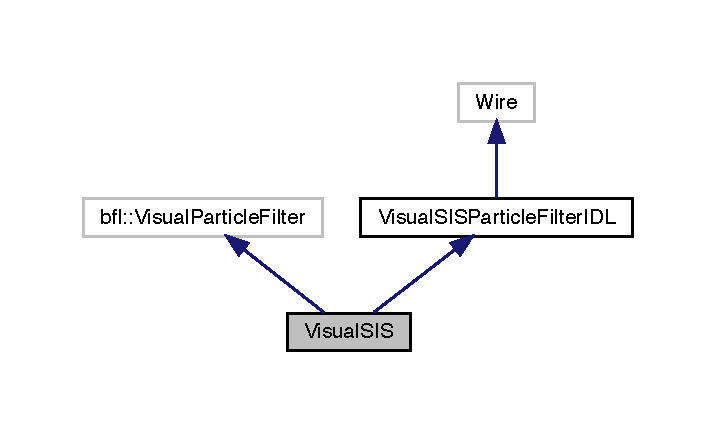
\includegraphics[width=344pt]{classVisualSIS__inherit__graph}
\end{center}
\end{figure}
\subsection*{Public Member Functions}
\begin{DoxyCompactItemize}
\item 
\hyperlink{classVisualSIS_a9088e9979575b7138557bbb02e81c59c}{Visual\+S\+IS} (const yarp\+::os\+::\+Const\+String \&cam\+\_\+sel, const int img\+\_\+width, const int img\+\_\+height, const int num\+\_\+particles, const double resample\+\_\+ratio)
\item 
\hyperlink{classVisualSIS_a9b57f7b419bd86a4528cbe87e6f53a14}{$\sim$\+Visual\+S\+IS} () noexcept
\item 
virtual bool \hyperlink{classVisualSISParticleFilterIDL_aade5ce77926faff0e94ffbf77f20c2c0}{read} (yarp\+::os\+::\+Connection\+Reader \&connection) override
\item 
virtual std\+::vector$<$ std\+::string $>$ \hyperlink{classVisualSISParticleFilterIDL_a3253f4dbc55e47183c04eb2e1054733c}{help} (const std\+::string \&function\+Name=\char`\"{}-\/-\/all\char`\"{})
\end{DoxyCompactItemize}
\subsection*{Protected Member Functions}
\begin{DoxyCompactItemize}
\item 
void \hyperlink{classVisualSIS_a324f4b8554036b0d697423ea7ab865be}{initialization} () override
\item 
void \hyperlink{classVisualSIS_a5c1e7ef8000c981db41cad3c6d17a535}{filtering\+Step} () override
\item 
void \hyperlink{classVisualSIS_a344387f214c60a62b2d79e7377f92693}{get\+Result} () override
\item 
bool \hyperlink{classVisualSIS_af053d8966ebebac8bf8eb8cfce4e4903}{run\+Condition} () override
\item 
bool \hyperlink{classVisualSIS_a2a331e2d6285cb48541df86dcc27b2c1}{attach} (yarp\+::os\+::\+Port \&source)
\item 
bool \hyperlink{classVisualSIS_aac85d36ec741ed93d1659ddf910f7a03}{set\+Command\+Port} ()
\item 
bool \hyperlink{classVisualSIS_aa8ad54a90c9f1f6ca673d8d61721b7be}{run\+\_\+filter} () override
\begin{DoxyCompactList}\small\item\em Initialize and run the visual S\+IR particle filter. \end{DoxyCompactList}\item 
bool \hyperlink{classVisualSIS_a974ca828135835ccb4a2c3b7635b2aea}{reset\+\_\+filter} () override
\begin{DoxyCompactList}\small\item\em Reset the visual S\+IR particle filter. \end{DoxyCompactList}\item 
bool \hyperlink{classVisualSIS_a8e111a001d0dd201a5f661c9ff226bc1}{stop\+\_\+filter} () override
\begin{DoxyCompactList}\small\item\em Stop and reset the S\+IR particle filter. \end{DoxyCompactList}\item 
bool \hyperlink{classVisualSIS_ac9905862d7198c5ae80f7e682500c608}{skip\+\_\+step} (const std\+::string \&what\+\_\+step, const bool status) override
\begin{DoxyCompactList}\small\item\em Enable/\+Disable skipping the filtering step specified in what\+\_\+step. \end{DoxyCompactList}\item 
bool \hyperlink{classVisualSIS_a703f84794cd66eb82040d2590b62f094}{use\+\_\+analogs} (const bool status) override
\begin{DoxyCompactList}\small\item\em Use/\+Don\textquotesingle{}t use the analog values from the right hand to correct the finger poses. \end{DoxyCompactList}\item 
std\+::vector$<$ std\+::string $>$ \hyperlink{classVisualSIS_af1ecb78ecc8c9838c05b7d29c5a9f83a}{get\+\_\+info} () override
\begin{DoxyCompactList}\small\item\em Get information about recursive Bayesian filter, like it\textquotesingle{}s status, the available methods, and the current one in use, to extract the state estimate from the particle set. \end{DoxyCompactList}\item 
bool \hyperlink{classVisualSIS_abff835a326f38e95187148d9401d5170}{quit} () override
\begin{DoxyCompactList}\small\item\em Gently close the application, deallocating resources. \end{DoxyCompactList}\item 
bool \hyperlink{classVisualSIS_ab45998859ed6c115eb0a8446f94c764e}{set\+\_\+estimates\+\_\+extraction\+\_\+method} (const std\+::string \&method) override
\begin{DoxyCompactList}\small\item\em Change the current method to extract the state estimates from the particle set. \end{DoxyCompactList}\item 
bool \hyperlink{classVisualSIS_a08aa7928cccabd93a1907cb540863cda}{set\+\_\+mobile\+\_\+average\+\_\+window} (const int16\+\_\+t window) override
\begin{DoxyCompactList}\small\item\em Change the window size of mobile averages for estimates extraction. \end{DoxyCompactList}\end{DoxyCompactItemize}
\subsection*{Protected Attributes}
\begin{DoxyCompactItemize}
\item 
yarp\+::os\+::\+Const\+String \hyperlink{classVisualSIS_a4ba71c5fa28e12504eea098298a28f66}{cam\+\_\+sel\+\_\+}
\item 
int \hyperlink{classVisualSIS_a1e168675500d9c8a949e8c2f69be1f5f}{img\+\_\+width\+\_\+}
\item 
int \hyperlink{classVisualSIS_aff43a51053f61e07a9803926111b9cc6}{img\+\_\+height\+\_\+}
\item 
int \hyperlink{classVisualSIS_af79e137085ec9c4764f5d7f8f0630cb5}{num\+\_\+particles\+\_\+}
\item 
unsigned int \hyperlink{classVisualSIS_a030a089e79e98f530082889b6d1d7090}{descriptor\+\_\+length\+\_\+}
\item 
double \hyperlink{classVisualSIS_a5e400fe8722793a0cc3a64900b30ff6a}{resample\+\_\+ratio\+\_\+}
\item 
const int \hyperlink{classVisualSIS_ae05ef520a7385930b44409f0ff83e99e}{block\+\_\+size\+\_\+} = 16
\item 
const int \hyperlink{classVisualSIS_a454d2a632bd8db7379882d61a85414bc}{bin\+\_\+number\+\_\+} = 9
\item 
cv\+::\+Ptr$<$ cv\+::cuda\+::\+H\+OG $>$ \hyperlink{classVisualSIS_aebdc06fc72c1e391c69bdcbd19fde848}{cuda\+\_\+hog\+\_\+}
\item 
yarp\+::os\+::\+Buffered\+Port$<$ yarp\+::sig\+::\+Vector $>$ \hyperlink{classVisualSIS_a844c2f19eef592ce79a3e56ee845b1bb}{port\+\_\+estimates\+\_\+out\+\_\+}
\item 
yarp\+::os\+::\+Buffered\+Port$<$ yarp\+::sig\+::\+Image\+Of$<$ yarp\+::sig\+::\+Pixel\+Rgb $>$ $>$ \hyperlink{classVisualSIS_ac45684c34e7413a13b6ed301cd8a7aa1}{port\+\_\+image\+\_\+in\+\_\+}
\item 
yarp\+::os\+::\+Port \hyperlink{classVisualSIS_ac08ca49836aaad57b7d5f7240a6d1ca5}{port\+\_\+rpc\+\_\+command\+\_\+}
\end{DoxyCompactItemize}
\subsection*{Private Attributes}
\begin{DoxyCompactItemize}
\item 
Eigen\+::\+Matrix\+Xf \hyperlink{classVisualSIS_accd71e6f7ced897e5b61e3b6c01243d4}{pred\+\_\+particle\+\_\+}
\item 
Eigen\+::\+Vector\+Xf \hyperlink{classVisualSIS_aa0251c7dd7c4d13a849b051145dbcc78}{pred\+\_\+weight\+\_\+}
\item 
Eigen\+::\+Matrix\+Xf \hyperlink{classVisualSIS_ab2f16295dc79084196a8cb5db6a3696e}{cor\+\_\+particle\+\_\+}
\item 
Eigen\+::\+Vector\+Xf \hyperlink{classVisualSIS_a497a31b9417a12005b6253bc100ab476}{cor\+\_\+weight\+\_\+}
\item 
bfl\+::\+Estimates\+Extraction \hyperlink{classVisualSIS_a5052345aafc5e7efc7d72f1ccbf0a4ac}{estimate\+\_\+extraction\+\_\+}
\item 
bool \hyperlink{classVisualSIS_abe30d9bbca8a9f6fde0140c10451ad05}{init\+\_\+img\+\_\+in\+\_\+} = false
\item 
yarp\+::sig\+::\+Image\+Of$<$ yarp\+::sig\+::\+Pixel\+Rgb $>$ \hyperlink{classVisualSIS_adde5e15abd023e42e940a77e4d096ba5}{img\+\_\+in\+\_\+}
\end{DoxyCompactItemize}


\subsection{Detailed Description}


Definition at line 26 of file Visual\+S\+I\+S.\+h.



\subsection{Constructor \& Destructor Documentation}
\mbox{\Hypertarget{classVisualSIS_a9088e9979575b7138557bbb02e81c59c}\label{classVisualSIS_a9088e9979575b7138557bbb02e81c59c}} 
\index{Visual\+S\+IS@{Visual\+S\+IS}!Visual\+S\+IS@{Visual\+S\+IS}}
\index{Visual\+S\+IS@{Visual\+S\+IS}!Visual\+S\+IS@{Visual\+S\+IS}}
\subsubsection{\texorpdfstring{Visual\+S\+I\+S()}{VisualSIS()}}
{\footnotesize\ttfamily Visual\+S\+I\+S\+::\+Visual\+S\+IS (\begin{DoxyParamCaption}\item[{const yarp\+::os\+::\+Const\+String \&}]{cam\+\_\+sel,  }\item[{const int}]{img\+\_\+width,  }\item[{const int}]{img\+\_\+height,  }\item[{const int}]{num\+\_\+particles,  }\item[{const double}]{resample\+\_\+ratio }\end{DoxyParamCaption})}



Definition at line 32 of file Visual\+S\+I\+S.\+cpp.



References bin\+\_\+number\+\_\+, block\+\_\+size\+\_\+, cam\+\_\+sel\+\_\+, cuda\+\_\+hog\+\_\+, descriptor\+\_\+length\+\_\+, img\+\_\+height\+\_\+, img\+\_\+in\+\_\+, img\+\_\+width\+\_\+, port\+\_\+estimates\+\_\+out\+\_\+, port\+\_\+image\+\_\+in\+\_\+, and set\+Command\+Port().

Here is the call graph for this function\+:
\nopagebreak
\begin{figure}[H]
\begin{center}
\leavevmode
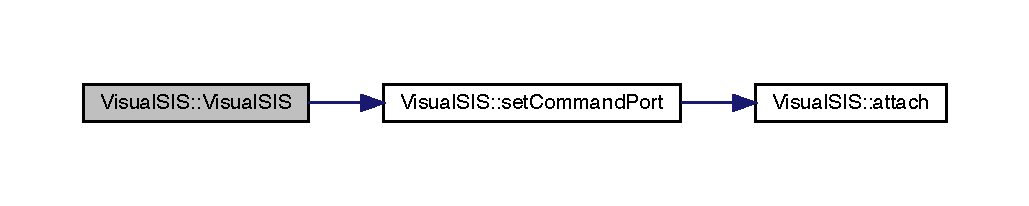
\includegraphics[width=350pt]{classVisualSIS_a9088e9979575b7138557bbb02e81c59c_cgraph}
\end{center}
\end{figure}
\mbox{\Hypertarget{classVisualSIS_a9b57f7b419bd86a4528cbe87e6f53a14}\label{classVisualSIS_a9b57f7b419bd86a4528cbe87e6f53a14}} 
\index{Visual\+S\+IS@{Visual\+S\+IS}!````~Visual\+S\+IS@{$\sim$\+Visual\+S\+IS}}
\index{````~Visual\+S\+IS@{$\sim$\+Visual\+S\+IS}!Visual\+S\+IS@{Visual\+S\+IS}}
\subsubsection{\texorpdfstring{$\sim$\+Visual\+S\+I\+S()}{~VisualSIS()}}
{\footnotesize\ttfamily Visual\+S\+I\+S\+::$\sim$\+Visual\+S\+IS (\begin{DoxyParamCaption}{ }\end{DoxyParamCaption})\hspace{0.3cm}{\ttfamily [noexcept]}}



Definition at line 79 of file Visual\+S\+I\+S.\+cpp.



References port\+\_\+estimates\+\_\+out\+\_\+, and port\+\_\+image\+\_\+in\+\_\+.



\subsection{Member Function Documentation}
\mbox{\Hypertarget{classVisualSIS_a2a331e2d6285cb48541df86dcc27b2c1}\label{classVisualSIS_a2a331e2d6285cb48541df86dcc27b2c1}} 
\index{Visual\+S\+IS@{Visual\+S\+IS}!attach@{attach}}
\index{attach@{attach}!Visual\+S\+IS@{Visual\+S\+IS}}
\subsubsection{\texorpdfstring{attach()}{attach()}}
{\footnotesize\ttfamily bool Visual\+S\+I\+S\+::attach (\begin{DoxyParamCaption}\item[{yarp\+::os\+::\+Port \&}]{source }\end{DoxyParamCaption})\hspace{0.3cm}{\ttfamily [protected]}}



Definition at line 209 of file Visual\+S\+I\+S.\+cpp.



Referenced by set\+Command\+Port().

\mbox{\Hypertarget{classVisualSIS_a5c1e7ef8000c981db41cad3c6d17a535}\label{classVisualSIS_a5c1e7ef8000c981db41cad3c6d17a535}} 
\index{Visual\+S\+IS@{Visual\+S\+IS}!filtering\+Step@{filtering\+Step}}
\index{filtering\+Step@{filtering\+Step}!Visual\+S\+IS@{Visual\+S\+IS}}
\subsubsection{\texorpdfstring{filtering\+Step()}{filteringStep()}}
{\footnotesize\ttfamily void Visual\+S\+I\+S\+::filtering\+Step (\begin{DoxyParamCaption}{ }\end{DoxyParamCaption})\hspace{0.3cm}{\ttfamily [override]}, {\ttfamily [protected]}}



Definition at line 86 of file Visual\+S\+I\+S.\+cpp.



References cor\+\_\+particle\+\_\+, cor\+\_\+weight\+\_\+, cuda\+\_\+hog\+\_\+, descriptor\+\_\+length\+\_\+, estimate\+\_\+extraction\+\_\+, img\+\_\+height\+\_\+, img\+\_\+in\+\_\+, img\+\_\+width\+\_\+, init\+\_\+img\+\_\+in\+\_\+, num\+\_\+particles\+\_\+, port\+\_\+estimates\+\_\+out\+\_\+, port\+\_\+image\+\_\+in\+\_\+, pred\+\_\+particle\+\_\+, pred\+\_\+weight\+\_\+, and resample\+\_\+ratio\+\_\+.

\mbox{\Hypertarget{classVisualSIS_af1ecb78ecc8c9838c05b7d29c5a9f83a}\label{classVisualSIS_af1ecb78ecc8c9838c05b7d29c5a9f83a}} 
\index{Visual\+S\+IS@{Visual\+S\+IS}!get\+\_\+info@{get\+\_\+info}}
\index{get\+\_\+info@{get\+\_\+info}!Visual\+S\+IS@{Visual\+S\+IS}}
\subsubsection{\texorpdfstring{get\+\_\+info()}{get\_info()}}
{\footnotesize\ttfamily std\+::vector$<$ std\+::string $>$ Visual\+S\+I\+S\+::get\+\_\+info (\begin{DoxyParamCaption}{ }\end{DoxyParamCaption})\hspace{0.3cm}{\ttfamily [override]}, {\ttfamily [protected]}, {\ttfamily [virtual]}}



Get information about recursive Bayesian filter, like it\textquotesingle{}s status, the available methods, and the current one in use, to extract the state estimate from the particle set. 

\begin{DoxyReturn}{Returns}
a string with all the available information, \textquotesingle{}none\textquotesingle{} otherwise 
\end{DoxyReturn}


Reimplemented from \hyperlink{classVisualSISParticleFilterIDL_a0721bc76b2d5848908a39e3a9c9740c0}{Visual\+S\+I\+S\+Particle\+Filter\+I\+DL}.



Definition at line 273 of file Visual\+S\+I\+S.\+cpp.



References cam\+\_\+sel\+\_\+, estimate\+\_\+extraction\+\_\+, and num\+\_\+particles\+\_\+.

\mbox{\Hypertarget{classVisualSIS_a344387f214c60a62b2d79e7377f92693}\label{classVisualSIS_a344387f214c60a62b2d79e7377f92693}} 
\index{Visual\+S\+IS@{Visual\+S\+IS}!get\+Result@{get\+Result}}
\index{get\+Result@{get\+Result}!Visual\+S\+IS@{Visual\+S\+IS}}
\subsubsection{\texorpdfstring{get\+Result()}{getResult()}}
{\footnotesize\ttfamily void Visual\+S\+I\+S\+::get\+Result (\begin{DoxyParamCaption}{ }\end{DoxyParamCaption})\hspace{0.3cm}{\ttfamily [override]}, {\ttfamily [protected]}}



Definition at line 206 of file Visual\+S\+I\+S.\+cpp.

\mbox{\Hypertarget{classVisualSISParticleFilterIDL_a3253f4dbc55e47183c04eb2e1054733c}\label{classVisualSISParticleFilterIDL_a3253f4dbc55e47183c04eb2e1054733c}} 
\index{Visual\+S\+IS@{Visual\+S\+IS}!help@{help}}
\index{help@{help}!Visual\+S\+IS@{Visual\+S\+IS}}
\subsubsection{\texorpdfstring{help()}{help()}}
{\footnotesize\ttfamily virtual std\+::vector$<$std\+::string$>$ Visual\+S\+I\+S\+Particle\+Filter\+I\+D\+L\+::help (\begin{DoxyParamCaption}\item[{const std\+::string \&}]{function\+Name = {\ttfamily \char`\"{}-\/-\/all\char`\"{}} }\end{DoxyParamCaption})\hspace{0.3cm}{\ttfamily [virtual]}, {\ttfamily [inherited]}}

\mbox{\Hypertarget{classVisualSIS_a324f4b8554036b0d697423ea7ab865be}\label{classVisualSIS_a324f4b8554036b0d697423ea7ab865be}} 
\index{Visual\+S\+IS@{Visual\+S\+IS}!initialization@{initialization}}
\index{initialization@{initialization}!Visual\+S\+IS@{Visual\+S\+IS}}
\subsubsection{\texorpdfstring{initialization()}{initialization()}}
{\footnotesize\ttfamily void Visual\+S\+I\+S\+::initialization (\begin{DoxyParamCaption}{ }\end{DoxyParamCaption})\hspace{0.3cm}{\ttfamily [override]}, {\ttfamily [protected]}}



Definition at line 61 of file Visual\+S\+I\+S.\+cpp.



References cor\+\_\+particle\+\_\+, cor\+\_\+weight\+\_\+, estimate\+\_\+extraction\+\_\+, num\+\_\+particles\+\_\+, pred\+\_\+particle\+\_\+, and pred\+\_\+weight\+\_\+.

\mbox{\Hypertarget{classVisualSIS_abff835a326f38e95187148d9401d5170}\label{classVisualSIS_abff835a326f38e95187148d9401d5170}} 
\index{Visual\+S\+IS@{Visual\+S\+IS}!quit@{quit}}
\index{quit@{quit}!Visual\+S\+IS@{Visual\+S\+IS}}
\subsubsection{\texorpdfstring{quit()}{quit()}}
{\footnotesize\ttfamily bool Visual\+S\+I\+S\+::quit (\begin{DoxyParamCaption}{ }\end{DoxyParamCaption})\hspace{0.3cm}{\ttfamily [override]}, {\ttfamily [protected]}, {\ttfamily [virtual]}}



Gently close the application, deallocating resources. 



Reimplemented from \hyperlink{classVisualSISParticleFilterIDL_a3f02a3df0d3dd545a6c62dc3a9f002b4}{Visual\+S\+I\+S\+Particle\+Filter\+I\+DL}.



Definition at line 355 of file Visual\+S\+I\+S.\+cpp.

\mbox{\Hypertarget{classVisualSISParticleFilterIDL_aade5ce77926faff0e94ffbf77f20c2c0}\label{classVisualSISParticleFilterIDL_aade5ce77926faff0e94ffbf77f20c2c0}} 
\index{Visual\+S\+IS@{Visual\+S\+IS}!read@{read}}
\index{read@{read}!Visual\+S\+IS@{Visual\+S\+IS}}
\subsubsection{\texorpdfstring{read()}{read()}}
{\footnotesize\ttfamily virtual bool Visual\+S\+I\+S\+Particle\+Filter\+I\+D\+L\+::read (\begin{DoxyParamCaption}\item[{yarp\+::os\+::\+Connection\+Reader \&}]{connection }\end{DoxyParamCaption})\hspace{0.3cm}{\ttfamily [override]}, {\ttfamily [virtual]}, {\ttfamily [inherited]}}

\mbox{\Hypertarget{classVisualSIS_a974ca828135835ccb4a2c3b7635b2aea}\label{classVisualSIS_a974ca828135835ccb4a2c3b7635b2aea}} 
\index{Visual\+S\+IS@{Visual\+S\+IS}!reset\+\_\+filter@{reset\+\_\+filter}}
\index{reset\+\_\+filter@{reset\+\_\+filter}!Visual\+S\+IS@{Visual\+S\+IS}}
\subsubsection{\texorpdfstring{reset\+\_\+filter()}{reset\_filter()}}
{\footnotesize\ttfamily bool Visual\+S\+I\+S\+::reset\+\_\+filter (\begin{DoxyParamCaption}{ }\end{DoxyParamCaption})\hspace{0.3cm}{\ttfamily [override]}, {\ttfamily [protected]}, {\ttfamily [virtual]}}



Reset the visual S\+IR particle filter. 

Returns upon successful or failure reset. \begin{DoxyReturn}{Returns}
true/false on success/failure. 
\end{DoxyReturn}


Reimplemented from \hyperlink{classVisualSISParticleFilterIDL_ad6047accd0fe743bdbd158cb9b6fc11b}{Visual\+S\+I\+S\+Particle\+Filter\+I\+DL}.



Definition at line 242 of file Visual\+S\+I\+S.\+cpp.

\mbox{\Hypertarget{classVisualSIS_aa8ad54a90c9f1f6ca673d8d61721b7be}\label{classVisualSIS_aa8ad54a90c9f1f6ca673d8d61721b7be}} 
\index{Visual\+S\+IS@{Visual\+S\+IS}!run\+\_\+filter@{run\+\_\+filter}}
\index{run\+\_\+filter@{run\+\_\+filter}!Visual\+S\+IS@{Visual\+S\+IS}}
\subsubsection{\texorpdfstring{run\+\_\+filter()}{run\_filter()}}
{\footnotesize\ttfamily bool Visual\+S\+I\+S\+::run\+\_\+filter (\begin{DoxyParamCaption}{ }\end{DoxyParamCaption})\hspace{0.3cm}{\ttfamily [override]}, {\ttfamily [protected]}, {\ttfamily [virtual]}}



Initialize and run the visual S\+IR particle filter. 

Returns upon successful or failure setup. \begin{DoxyReturn}{Returns}
true/false on success/failure. 
\end{DoxyReturn}


Reimplemented from \hyperlink{classVisualSISParticleFilterIDL_a6a8c16192597ea78617f10691b07df08}{Visual\+S\+I\+S\+Particle\+Filter\+I\+DL}.



Definition at line 234 of file Visual\+S\+I\+S.\+cpp.

\mbox{\Hypertarget{classVisualSIS_af053d8966ebebac8bf8eb8cfce4e4903}\label{classVisualSIS_af053d8966ebebac8bf8eb8cfce4e4903}} 
\index{Visual\+S\+IS@{Visual\+S\+IS}!run\+Condition@{run\+Condition}}
\index{run\+Condition@{run\+Condition}!Visual\+S\+IS@{Visual\+S\+IS}}
\subsubsection{\texorpdfstring{run\+Condition()}{runCondition()}}
{\footnotesize\ttfamily bool Visual\+S\+I\+S\+::run\+Condition (\begin{DoxyParamCaption}{ }\end{DoxyParamCaption})\hspace{0.3cm}{\ttfamily [inline]}, {\ttfamily [override]}, {\ttfamily [protected]}}



Definition at line 44 of file Visual\+S\+I\+S.\+h.



References cam\+\_\+sel\+\_\+.

\mbox{\Hypertarget{classVisualSIS_ab45998859ed6c115eb0a8446f94c764e}\label{classVisualSIS_ab45998859ed6c115eb0a8446f94c764e}} 
\index{Visual\+S\+IS@{Visual\+S\+IS}!set\+\_\+estimates\+\_\+extraction\+\_\+method@{set\+\_\+estimates\+\_\+extraction\+\_\+method}}
\index{set\+\_\+estimates\+\_\+extraction\+\_\+method@{set\+\_\+estimates\+\_\+extraction\+\_\+method}!Visual\+S\+IS@{Visual\+S\+IS}}
\subsubsection{\texorpdfstring{set\+\_\+estimates\+\_\+extraction\+\_\+method()}{set\_estimates\_extraction\_method()}}
{\footnotesize\ttfamily bool Visual\+S\+I\+S\+::set\+\_\+estimates\+\_\+extraction\+\_\+method (\begin{DoxyParamCaption}\item[{const std\+::string \&}]{method }\end{DoxyParamCaption})\hspace{0.3cm}{\ttfamily [override]}, {\ttfamily [protected]}, {\ttfamily [virtual]}}



Change the current method to extract the state estimates from the particle set. 


\begin{DoxyParams}{Parameters}
{\em status} & a string with the state estimate extraction method to use; the string shall be one of the available methods returned by the \hyperlink{classVisualSIS_af1ecb78ecc8c9838c05b7d29c5a9f83a}{get\+\_\+info()} method. \\
\hline
\end{DoxyParams}
\begin{DoxyReturn}{Returns}
true method changed successfully, false otherwise. 
\end{DoxyReturn}


Reimplemented from \hyperlink{classVisualSISParticleFilterIDL_ac5f296082bd83e1ee1b74e9af16e856a}{Visual\+S\+I\+S\+Particle\+Filter\+I\+DL}.



Definition at line 291 of file Visual\+S\+I\+S.\+cpp.



References estimate\+\_\+extraction\+\_\+.

\mbox{\Hypertarget{classVisualSIS_a08aa7928cccabd93a1907cb540863cda}\label{classVisualSIS_a08aa7928cccabd93a1907cb540863cda}} 
\index{Visual\+S\+IS@{Visual\+S\+IS}!set\+\_\+mobile\+\_\+average\+\_\+window@{set\+\_\+mobile\+\_\+average\+\_\+window}}
\index{set\+\_\+mobile\+\_\+average\+\_\+window@{set\+\_\+mobile\+\_\+average\+\_\+window}!Visual\+S\+IS@{Visual\+S\+IS}}
\subsubsection{\texorpdfstring{set\+\_\+mobile\+\_\+average\+\_\+window()}{set\_mobile\_average\_window()}}
{\footnotesize\ttfamily bool Visual\+S\+I\+S\+::set\+\_\+mobile\+\_\+average\+\_\+window (\begin{DoxyParamCaption}\item[{const int16\+\_\+t}]{window }\end{DoxyParamCaption})\hspace{0.3cm}{\ttfamily [override]}, {\ttfamily [protected]}, {\ttfamily [virtual]}}



Change the window size of mobile averages for estimates extraction. 


\begin{DoxyParams}{Parameters}
{\em window} & specifies the mobile window size. \\
\hline
\end{DoxyParams}
\begin{DoxyReturn}{Returns}
true window size changed successfully, false otherwise. 
\end{DoxyReturn}
\begin{DoxyNote}{Note}
The default value is 20. Minimum value is 2. Maximum value is 90. 
\end{DoxyNote}


Reimplemented from \hyperlink{classVisualSISParticleFilterIDL_a40d91826291e2bae76f4545254307577}{Visual\+S\+I\+S\+Particle\+Filter\+I\+DL}.



Definition at line 346 of file Visual\+S\+I\+S.\+cpp.



References estimate\+\_\+extraction\+\_\+.

\mbox{\Hypertarget{classVisualSIS_aac85d36ec741ed93d1659ddf910f7a03}\label{classVisualSIS_aac85d36ec741ed93d1659ddf910f7a03}} 
\index{Visual\+S\+IS@{Visual\+S\+IS}!set\+Command\+Port@{set\+Command\+Port}}
\index{set\+Command\+Port@{set\+Command\+Port}!Visual\+S\+IS@{Visual\+S\+IS}}
\subsubsection{\texorpdfstring{set\+Command\+Port()}{setCommandPort()}}
{\footnotesize\ttfamily bool Visual\+S\+I\+S\+::set\+Command\+Port (\begin{DoxyParamCaption}{ }\end{DoxyParamCaption})\hspace{0.3cm}{\ttfamily [protected]}}



Definition at line 215 of file Visual\+S\+I\+S.\+cpp.



References attach(), cam\+\_\+sel\+\_\+, and port\+\_\+rpc\+\_\+command\+\_\+.



Referenced by Visual\+S\+I\+S().

Here is the call graph for this function\+:
\nopagebreak
\begin{figure}[H]
\begin{center}
\leavevmode
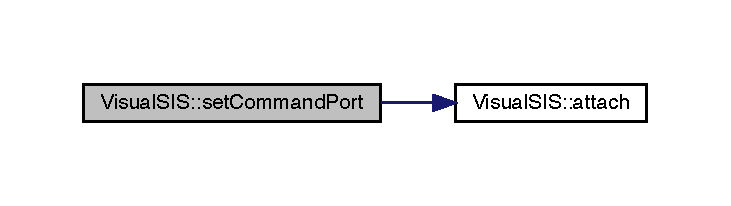
\includegraphics[width=350pt]{classVisualSIS_aac85d36ec741ed93d1659ddf910f7a03_cgraph}
\end{center}
\end{figure}
\mbox{\Hypertarget{classVisualSIS_ac9905862d7198c5ae80f7e682500c608}\label{classVisualSIS_ac9905862d7198c5ae80f7e682500c608}} 
\index{Visual\+S\+IS@{Visual\+S\+IS}!skip\+\_\+step@{skip\+\_\+step}}
\index{skip\+\_\+step@{skip\+\_\+step}!Visual\+S\+IS@{Visual\+S\+IS}}
\subsubsection{\texorpdfstring{skip\+\_\+step()}{skip\_step()}}
{\footnotesize\ttfamily bool Visual\+S\+I\+S\+::skip\+\_\+step (\begin{DoxyParamCaption}\item[{const std\+::string \&}]{what\+\_\+step,  }\item[{const bool}]{status }\end{DoxyParamCaption})\hspace{0.3cm}{\ttfamily [override]}, {\ttfamily [protected]}, {\ttfamily [virtual]}}



Enable/\+Disable skipping the filtering step specified in what\+\_\+step. 

what\+\_\+step can be one of the following\+: 1) prediction\+: skips the whole prediction step 2) state\+: skips the prediction step related to the state transition 3) exogenous\+: skips the prediction step related exogenous inputs 4) correction\+: skips the whole correction step 
\begin{DoxyParams}{Parameters}
{\em what\+\_\+step} & the step to skipping \\
\hline
{\em status} & enable/disable skipping \\
\hline
\end{DoxyParams}
\begin{DoxyReturn}{Returns}
true/false on success/failure. 
\end{DoxyReturn}


Reimplemented from \hyperlink{classVisualSISParticleFilterIDL_a09d343c25082f2056546c6e95d397eaf}{Visual\+S\+I\+S\+Particle\+Filter\+I\+DL}.



Definition at line 258 of file Visual\+S\+I\+S.\+cpp.

\mbox{\Hypertarget{classVisualSIS_a8e111a001d0dd201a5f661c9ff226bc1}\label{classVisualSIS_a8e111a001d0dd201a5f661c9ff226bc1}} 
\index{Visual\+S\+IS@{Visual\+S\+IS}!stop\+\_\+filter@{stop\+\_\+filter}}
\index{stop\+\_\+filter@{stop\+\_\+filter}!Visual\+S\+IS@{Visual\+S\+IS}}
\subsubsection{\texorpdfstring{stop\+\_\+filter()}{stop\_filter()}}
{\footnotesize\ttfamily bool Visual\+S\+I\+S\+::stop\+\_\+filter (\begin{DoxyParamCaption}{ }\end{DoxyParamCaption})\hspace{0.3cm}{\ttfamily [override]}, {\ttfamily [protected]}, {\ttfamily [virtual]}}



Stop and reset the S\+IR particle filter. 

This method must be called when the S\+IR particle filter is no longer needed or a new filtering task need to be initialized. \begin{DoxyReturn}{Returns}
true/false on success/failure. 
\end{DoxyReturn}


Reimplemented from \hyperlink{classVisualSISParticleFilterIDL_a8a30501c75b4c7152a2abff96a950b63}{Visual\+S\+I\+S\+Particle\+Filter\+I\+DL}.



Definition at line 250 of file Visual\+S\+I\+S.\+cpp.

\mbox{\Hypertarget{classVisualSIS_a703f84794cd66eb82040d2590b62f094}\label{classVisualSIS_a703f84794cd66eb82040d2590b62f094}} 
\index{Visual\+S\+IS@{Visual\+S\+IS}!use\+\_\+analogs@{use\+\_\+analogs}}
\index{use\+\_\+analogs@{use\+\_\+analogs}!Visual\+S\+IS@{Visual\+S\+IS}}
\subsubsection{\texorpdfstring{use\+\_\+analogs()}{use\_analogs()}}
{\footnotesize\ttfamily bool Visual\+S\+I\+S\+::use\+\_\+analogs (\begin{DoxyParamCaption}\item[{const bool}]{status }\end{DoxyParamCaption})\hspace{0.3cm}{\ttfamily [override]}, {\ttfamily [protected]}, {\ttfamily [virtual]}}



Use/\+Don\textquotesingle{}t use the analog values from the right hand to correct the finger poses. 


\begin{DoxyParams}{Parameters}
{\em status} & true/false to use/don\textquotesingle{}t use analog values. \\
\hline
\end{DoxyParams}
\begin{DoxyReturn}{Returns}
true activation/deactivation success, false otherwise. 
\end{DoxyReturn}


Reimplemented from \hyperlink{classVisualSISParticleFilterIDL_a4fee3e1fbc6676767f99c8b552434709}{Visual\+S\+I\+S\+Particle\+Filter\+I\+DL}.



Definition at line 264 of file Visual\+S\+I\+S.\+cpp.



\subsection{Member Data Documentation}
\mbox{\Hypertarget{classVisualSIS_a454d2a632bd8db7379882d61a85414bc}\label{classVisualSIS_a454d2a632bd8db7379882d61a85414bc}} 
\index{Visual\+S\+IS@{Visual\+S\+IS}!bin\+\_\+number\+\_\+@{bin\+\_\+number\+\_\+}}
\index{bin\+\_\+number\+\_\+@{bin\+\_\+number\+\_\+}!Visual\+S\+IS@{Visual\+S\+IS}}
\subsubsection{\texorpdfstring{bin\+\_\+number\+\_\+}{bin\_number\_}}
{\footnotesize\ttfamily const int Visual\+S\+I\+S\+::bin\+\_\+number\+\_\+ = 9\hspace{0.3cm}{\ttfamily [protected]}}



Definition at line 55 of file Visual\+S\+I\+S.\+h.



Referenced by Visual\+S\+I\+S().

\mbox{\Hypertarget{classVisualSIS_ae05ef520a7385930b44409f0ff83e99e}\label{classVisualSIS_ae05ef520a7385930b44409f0ff83e99e}} 
\index{Visual\+S\+IS@{Visual\+S\+IS}!block\+\_\+size\+\_\+@{block\+\_\+size\+\_\+}}
\index{block\+\_\+size\+\_\+@{block\+\_\+size\+\_\+}!Visual\+S\+IS@{Visual\+S\+IS}}
\subsubsection{\texorpdfstring{block\+\_\+size\+\_\+}{block\_size\_}}
{\footnotesize\ttfamily const int Visual\+S\+I\+S\+::block\+\_\+size\+\_\+ = 16\hspace{0.3cm}{\ttfamily [protected]}}



Definition at line 54 of file Visual\+S\+I\+S.\+h.



Referenced by Visual\+S\+I\+S().

\mbox{\Hypertarget{classVisualSIS_a4ba71c5fa28e12504eea098298a28f66}\label{classVisualSIS_a4ba71c5fa28e12504eea098298a28f66}} 
\index{Visual\+S\+IS@{Visual\+S\+IS}!cam\+\_\+sel\+\_\+@{cam\+\_\+sel\+\_\+}}
\index{cam\+\_\+sel\+\_\+@{cam\+\_\+sel\+\_\+}!Visual\+S\+IS@{Visual\+S\+IS}}
\subsubsection{\texorpdfstring{cam\+\_\+sel\+\_\+}{cam\_sel\_}}
{\footnotesize\ttfamily yarp\+::os\+::\+Const\+String Visual\+S\+I\+S\+::cam\+\_\+sel\+\_\+\hspace{0.3cm}{\ttfamily [protected]}}



Definition at line 44 of file Visual\+S\+I\+S.\+h.



Referenced by get\+\_\+info(), run\+Condition(), set\+Command\+Port(), and Visual\+S\+I\+S().

\mbox{\Hypertarget{classVisualSIS_ab2f16295dc79084196a8cb5db6a3696e}\label{classVisualSIS_ab2f16295dc79084196a8cb5db6a3696e}} 
\index{Visual\+S\+IS@{Visual\+S\+IS}!cor\+\_\+particle\+\_\+@{cor\+\_\+particle\+\_\+}}
\index{cor\+\_\+particle\+\_\+@{cor\+\_\+particle\+\_\+}!Visual\+S\+IS@{Visual\+S\+IS}}
\subsubsection{\texorpdfstring{cor\+\_\+particle\+\_\+}{cor\_particle\_}}
{\footnotesize\ttfamily Eigen\+::\+Matrix\+Xf Visual\+S\+I\+S\+::cor\+\_\+particle\+\_\+\hspace{0.3cm}{\ttfamily [private]}}



Definition at line 92 of file Visual\+S\+I\+S.\+h.



Referenced by filtering\+Step(), and initialization().

\mbox{\Hypertarget{classVisualSIS_a497a31b9417a12005b6253bc100ab476}\label{classVisualSIS_a497a31b9417a12005b6253bc100ab476}} 
\index{Visual\+S\+IS@{Visual\+S\+IS}!cor\+\_\+weight\+\_\+@{cor\+\_\+weight\+\_\+}}
\index{cor\+\_\+weight\+\_\+@{cor\+\_\+weight\+\_\+}!Visual\+S\+IS@{Visual\+S\+IS}}
\subsubsection{\texorpdfstring{cor\+\_\+weight\+\_\+}{cor\_weight\_}}
{\footnotesize\ttfamily Eigen\+::\+Vector\+Xf Visual\+S\+I\+S\+::cor\+\_\+weight\+\_\+\hspace{0.3cm}{\ttfamily [private]}}



Definition at line 93 of file Visual\+S\+I\+S.\+h.



Referenced by filtering\+Step(), and initialization().

\mbox{\Hypertarget{classVisualSIS_aebdc06fc72c1e391c69bdcbd19fde848}\label{classVisualSIS_aebdc06fc72c1e391c69bdcbd19fde848}} 
\index{Visual\+S\+IS@{Visual\+S\+IS}!cuda\+\_\+hog\+\_\+@{cuda\+\_\+hog\+\_\+}}
\index{cuda\+\_\+hog\+\_\+@{cuda\+\_\+hog\+\_\+}!Visual\+S\+IS@{Visual\+S\+IS}}
\subsubsection{\texorpdfstring{cuda\+\_\+hog\+\_\+}{cuda\_hog\_}}
{\footnotesize\ttfamily cv\+::\+Ptr$<$cv\+::cuda\+::\+H\+OG$>$ Visual\+S\+I\+S\+::cuda\+\_\+hog\+\_\+\hspace{0.3cm}{\ttfamily [protected]}}



Definition at line 57 of file Visual\+S\+I\+S.\+h.



Referenced by filtering\+Step(), and Visual\+S\+I\+S().

\mbox{\Hypertarget{classVisualSIS_a030a089e79e98f530082889b6d1d7090}\label{classVisualSIS_a030a089e79e98f530082889b6d1d7090}} 
\index{Visual\+S\+IS@{Visual\+S\+IS}!descriptor\+\_\+length\+\_\+@{descriptor\+\_\+length\+\_\+}}
\index{descriptor\+\_\+length\+\_\+@{descriptor\+\_\+length\+\_\+}!Visual\+S\+IS@{Visual\+S\+IS}}
\subsubsection{\texorpdfstring{descriptor\+\_\+length\+\_\+}{descriptor\_length\_}}
{\footnotesize\ttfamily unsigned int Visual\+S\+I\+S\+::descriptor\+\_\+length\+\_\+\hspace{0.3cm}{\ttfamily [protected]}}



Definition at line 51 of file Visual\+S\+I\+S.\+h.



Referenced by filtering\+Step(), and Visual\+S\+I\+S().

\mbox{\Hypertarget{classVisualSIS_a5052345aafc5e7efc7d72f1ccbf0a4ac}\label{classVisualSIS_a5052345aafc5e7efc7d72f1ccbf0a4ac}} 
\index{Visual\+S\+IS@{Visual\+S\+IS}!estimate\+\_\+extraction\+\_\+@{estimate\+\_\+extraction\+\_\+}}
\index{estimate\+\_\+extraction\+\_\+@{estimate\+\_\+extraction\+\_\+}!Visual\+S\+IS@{Visual\+S\+IS}}
\subsubsection{\texorpdfstring{estimate\+\_\+extraction\+\_\+}{estimate\_extraction\_}}
{\footnotesize\ttfamily bfl\+::\+Estimates\+Extraction Visual\+S\+I\+S\+::estimate\+\_\+extraction\+\_\+\hspace{0.3cm}{\ttfamily [private]}}



Definition at line 96 of file Visual\+S\+I\+S.\+h.



Referenced by filtering\+Step(), get\+\_\+info(), initialization(), set\+\_\+estimates\+\_\+extraction\+\_\+method(), and set\+\_\+mobile\+\_\+average\+\_\+window().

\mbox{\Hypertarget{classVisualSIS_aff43a51053f61e07a9803926111b9cc6}\label{classVisualSIS_aff43a51053f61e07a9803926111b9cc6}} 
\index{Visual\+S\+IS@{Visual\+S\+IS}!img\+\_\+height\+\_\+@{img\+\_\+height\+\_\+}}
\index{img\+\_\+height\+\_\+@{img\+\_\+height\+\_\+}!Visual\+S\+IS@{Visual\+S\+IS}}
\subsubsection{\texorpdfstring{img\+\_\+height\+\_\+}{img\_height\_}}
{\footnotesize\ttfamily int Visual\+S\+I\+S\+::img\+\_\+height\+\_\+\hspace{0.3cm}{\ttfamily [protected]}}



Definition at line 49 of file Visual\+S\+I\+S.\+h.



Referenced by filtering\+Step(), and Visual\+S\+I\+S().

\mbox{\Hypertarget{classVisualSIS_adde5e15abd023e42e940a77e4d096ba5}\label{classVisualSIS_adde5e15abd023e42e940a77e4d096ba5}} 
\index{Visual\+S\+IS@{Visual\+S\+IS}!img\+\_\+in\+\_\+@{img\+\_\+in\+\_\+}}
\index{img\+\_\+in\+\_\+@{img\+\_\+in\+\_\+}!Visual\+S\+IS@{Visual\+S\+IS}}
\subsubsection{\texorpdfstring{img\+\_\+in\+\_\+}{img\_in\_}}
{\footnotesize\ttfamily yarp\+::sig\+::\+Image\+Of$<$yarp\+::sig\+::\+Pixel\+Rgb$>$ Visual\+S\+I\+S\+::img\+\_\+in\+\_\+\hspace{0.3cm}{\ttfamily [private]}}



Definition at line 100 of file Visual\+S\+I\+S.\+h.



Referenced by filtering\+Step(), and Visual\+S\+I\+S().

\mbox{\Hypertarget{classVisualSIS_a1e168675500d9c8a949e8c2f69be1f5f}\label{classVisualSIS_a1e168675500d9c8a949e8c2f69be1f5f}} 
\index{Visual\+S\+IS@{Visual\+S\+IS}!img\+\_\+width\+\_\+@{img\+\_\+width\+\_\+}}
\index{img\+\_\+width\+\_\+@{img\+\_\+width\+\_\+}!Visual\+S\+IS@{Visual\+S\+IS}}
\subsubsection{\texorpdfstring{img\+\_\+width\+\_\+}{img\_width\_}}
{\footnotesize\ttfamily int Visual\+S\+I\+S\+::img\+\_\+width\+\_\+\hspace{0.3cm}{\ttfamily [protected]}}



Definition at line 48 of file Visual\+S\+I\+S.\+h.



Referenced by filtering\+Step(), and Visual\+S\+I\+S().

\mbox{\Hypertarget{classVisualSIS_abe30d9bbca8a9f6fde0140c10451ad05}\label{classVisualSIS_abe30d9bbca8a9f6fde0140c10451ad05}} 
\index{Visual\+S\+IS@{Visual\+S\+IS}!init\+\_\+img\+\_\+in\+\_\+@{init\+\_\+img\+\_\+in\+\_\+}}
\index{init\+\_\+img\+\_\+in\+\_\+@{init\+\_\+img\+\_\+in\+\_\+}!Visual\+S\+IS@{Visual\+S\+IS}}
\subsubsection{\texorpdfstring{init\+\_\+img\+\_\+in\+\_\+}{init\_img\_in\_}}
{\footnotesize\ttfamily bool Visual\+S\+I\+S\+::init\+\_\+img\+\_\+in\+\_\+ = false\hspace{0.3cm}{\ttfamily [private]}}



Definition at line 99 of file Visual\+S\+I\+S.\+h.



Referenced by filtering\+Step().

\mbox{\Hypertarget{classVisualSIS_af79e137085ec9c4764f5d7f8f0630cb5}\label{classVisualSIS_af79e137085ec9c4764f5d7f8f0630cb5}} 
\index{Visual\+S\+IS@{Visual\+S\+IS}!num\+\_\+particles\+\_\+@{num\+\_\+particles\+\_\+}}
\index{num\+\_\+particles\+\_\+@{num\+\_\+particles\+\_\+}!Visual\+S\+IS@{Visual\+S\+IS}}
\subsubsection{\texorpdfstring{num\+\_\+particles\+\_\+}{num\_particles\_}}
{\footnotesize\ttfamily int Visual\+S\+I\+S\+::num\+\_\+particles\+\_\+\hspace{0.3cm}{\ttfamily [protected]}}



Definition at line 50 of file Visual\+S\+I\+S.\+h.



Referenced by filtering\+Step(), get\+\_\+info(), and initialization().

\mbox{\Hypertarget{classVisualSIS_a844c2f19eef592ce79a3e56ee845b1bb}\label{classVisualSIS_a844c2f19eef592ce79a3e56ee845b1bb}} 
\index{Visual\+S\+IS@{Visual\+S\+IS}!port\+\_\+estimates\+\_\+out\+\_\+@{port\+\_\+estimates\+\_\+out\+\_\+}}
\index{port\+\_\+estimates\+\_\+out\+\_\+@{port\+\_\+estimates\+\_\+out\+\_\+}!Visual\+S\+IS@{Visual\+S\+IS}}
\subsubsection{\texorpdfstring{port\+\_\+estimates\+\_\+out\+\_\+}{port\_estimates\_out\_}}
{\footnotesize\ttfamily yarp\+::os\+::\+Buffered\+Port$<$yarp\+::sig\+::\+Vector$>$ Visual\+S\+I\+S\+::port\+\_\+estimates\+\_\+out\+\_\+\hspace{0.3cm}{\ttfamily [protected]}}



Definition at line 60 of file Visual\+S\+I\+S.\+h.



Referenced by filtering\+Step(), Visual\+S\+I\+S(), and $\sim$\+Visual\+S\+I\+S().

\mbox{\Hypertarget{classVisualSIS_ac45684c34e7413a13b6ed301cd8a7aa1}\label{classVisualSIS_ac45684c34e7413a13b6ed301cd8a7aa1}} 
\index{Visual\+S\+IS@{Visual\+S\+IS}!port\+\_\+image\+\_\+in\+\_\+@{port\+\_\+image\+\_\+in\+\_\+}}
\index{port\+\_\+image\+\_\+in\+\_\+@{port\+\_\+image\+\_\+in\+\_\+}!Visual\+S\+IS@{Visual\+S\+IS}}
\subsubsection{\texorpdfstring{port\+\_\+image\+\_\+in\+\_\+}{port\_image\_in\_}}
{\footnotesize\ttfamily yarp\+::os\+::\+Buffered\+Port$<$yarp\+::sig\+::\+Image\+Of$<$yarp\+::sig\+::\+Pixel\+Rgb$>$ $>$ Visual\+S\+I\+S\+::port\+\_\+image\+\_\+in\+\_\+\hspace{0.3cm}{\ttfamily [protected]}}



Definition at line 61 of file Visual\+S\+I\+S.\+h.



Referenced by filtering\+Step(), Visual\+S\+I\+S(), and $\sim$\+Visual\+S\+I\+S().

\mbox{\Hypertarget{classVisualSIS_ac08ca49836aaad57b7d5f7240a6d1ca5}\label{classVisualSIS_ac08ca49836aaad57b7d5f7240a6d1ca5}} 
\index{Visual\+S\+IS@{Visual\+S\+IS}!port\+\_\+rpc\+\_\+command\+\_\+@{port\+\_\+rpc\+\_\+command\+\_\+}}
\index{port\+\_\+rpc\+\_\+command\+\_\+@{port\+\_\+rpc\+\_\+command\+\_\+}!Visual\+S\+IS@{Visual\+S\+IS}}
\subsubsection{\texorpdfstring{port\+\_\+rpc\+\_\+command\+\_\+}{port\_rpc\_command\_}}
{\footnotesize\ttfamily yarp\+::os\+::\+Port Visual\+S\+I\+S\+::port\+\_\+rpc\+\_\+command\+\_\+\hspace{0.3cm}{\ttfamily [protected]}}



Definition at line 64 of file Visual\+S\+I\+S.\+h.



Referenced by set\+Command\+Port().

\mbox{\Hypertarget{classVisualSIS_accd71e6f7ced897e5b61e3b6c01243d4}\label{classVisualSIS_accd71e6f7ced897e5b61e3b6c01243d4}} 
\index{Visual\+S\+IS@{Visual\+S\+IS}!pred\+\_\+particle\+\_\+@{pred\+\_\+particle\+\_\+}}
\index{pred\+\_\+particle\+\_\+@{pred\+\_\+particle\+\_\+}!Visual\+S\+IS@{Visual\+S\+IS}}
\subsubsection{\texorpdfstring{pred\+\_\+particle\+\_\+}{pred\_particle\_}}
{\footnotesize\ttfamily Eigen\+::\+Matrix\+Xf Visual\+S\+I\+S\+::pred\+\_\+particle\+\_\+\hspace{0.3cm}{\ttfamily [private]}}



Definition at line 89 of file Visual\+S\+I\+S.\+h.



Referenced by filtering\+Step(), and initialization().

\mbox{\Hypertarget{classVisualSIS_aa0251c7dd7c4d13a849b051145dbcc78}\label{classVisualSIS_aa0251c7dd7c4d13a849b051145dbcc78}} 
\index{Visual\+S\+IS@{Visual\+S\+IS}!pred\+\_\+weight\+\_\+@{pred\+\_\+weight\+\_\+}}
\index{pred\+\_\+weight\+\_\+@{pred\+\_\+weight\+\_\+}!Visual\+S\+IS@{Visual\+S\+IS}}
\subsubsection{\texorpdfstring{pred\+\_\+weight\+\_\+}{pred\_weight\_}}
{\footnotesize\ttfamily Eigen\+::\+Vector\+Xf Visual\+S\+I\+S\+::pred\+\_\+weight\+\_\+\hspace{0.3cm}{\ttfamily [private]}}



Definition at line 90 of file Visual\+S\+I\+S.\+h.



Referenced by filtering\+Step(), and initialization().

\mbox{\Hypertarget{classVisualSIS_a5e400fe8722793a0cc3a64900b30ff6a}\label{classVisualSIS_a5e400fe8722793a0cc3a64900b30ff6a}} 
\index{Visual\+S\+IS@{Visual\+S\+IS}!resample\+\_\+ratio\+\_\+@{resample\+\_\+ratio\+\_\+}}
\index{resample\+\_\+ratio\+\_\+@{resample\+\_\+ratio\+\_\+}!Visual\+S\+IS@{Visual\+S\+IS}}
\subsubsection{\texorpdfstring{resample\+\_\+ratio\+\_\+}{resample\_ratio\_}}
{\footnotesize\ttfamily double Visual\+S\+I\+S\+::resample\+\_\+ratio\+\_\+\hspace{0.3cm}{\ttfamily [protected]}}



Definition at line 52 of file Visual\+S\+I\+S.\+h.



Referenced by filtering\+Step().



The documentation for this class was generated from the following files\+:\begin{DoxyCompactItemize}
\item 
/\+Users/\+Claudio/\+Git\+Hub/visual-\/tracking-\/control/src/hand-\/tracking/include/\hyperlink{VisualSIS_8h}{Visual\+S\+I\+S.\+h}\item 
/\+Users/\+Claudio/\+Git\+Hub/visual-\/tracking-\/control/src/hand-\/tracking/src/\hyperlink{VisualSIS_8cpp}{Visual\+S\+I\+S.\+cpp}\end{DoxyCompactItemize}

\hypertarget{classVisualSISParticleFilterIDL}{}\section{Visual\+S\+I\+S\+Particle\+Filter\+I\+DL Class Reference}
\label{classVisualSISParticleFilterIDL}\index{Visual\+S\+I\+S\+Particle\+Filter\+I\+DL@{Visual\+S\+I\+S\+Particle\+Filter\+I\+DL}}


\hyperlink{classVisualSISParticleFilterIDL}{Visual\+S\+I\+S\+Particle\+Filter\+I\+DL} I\+DL Interface to Visual\+S\+I\+R\+Particle\+Filter options.  




{\ttfamily \#include $<$Visual\+S\+I\+S\+Particle\+Filter\+I\+D\+L.\+h$>$}



Inheritance diagram for Visual\+S\+I\+S\+Particle\+Filter\+I\+DL\+:
\nopagebreak
\begin{figure}[H]
\begin{center}
\leavevmode
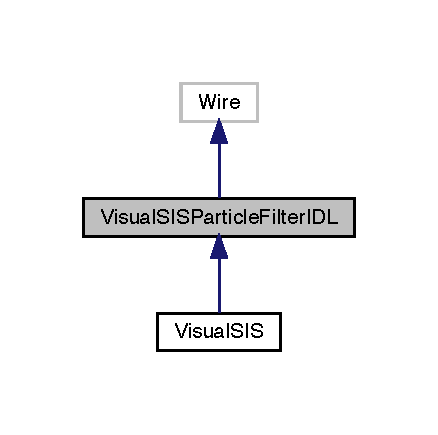
\includegraphics[width=210pt]{classVisualSISParticleFilterIDL__inherit__graph}
\end{center}
\end{figure}
\subsection*{Public Member Functions}
\begin{DoxyCompactItemize}
\item 
\hyperlink{classVisualSISParticleFilterIDL_ae295be0ced0b306a7b2a27e4b5e4df60}{Visual\+S\+I\+S\+Particle\+Filter\+I\+DL} ()
\item 
virtual bool \hyperlink{classVisualSISParticleFilterIDL_a6a8c16192597ea78617f10691b07df08}{run\+\_\+filter} ()
\begin{DoxyCompactList}\small\item\em Initialize and run the visual S\+IR particle filter. \end{DoxyCompactList}\item 
virtual bool \hyperlink{classVisualSISParticleFilterIDL_ad6047accd0fe743bdbd158cb9b6fc11b}{reset\+\_\+filter} ()
\begin{DoxyCompactList}\small\item\em Reset the visual S\+IR particle filter. \end{DoxyCompactList}\item 
virtual bool \hyperlink{classVisualSISParticleFilterIDL_a8a30501c75b4c7152a2abff96a950b63}{stop\+\_\+filter} ()
\begin{DoxyCompactList}\small\item\em Stop and reset the S\+IR particle filter. \end{DoxyCompactList}\item 
virtual bool \hyperlink{classVisualSISParticleFilterIDL_a09d343c25082f2056546c6e95d397eaf}{skip\+\_\+step} (const std\+::string \&what\+\_\+step, const bool status)
\begin{DoxyCompactList}\small\item\em Enable/\+Disable skipping the filtering step specified in what\+\_\+step. \end{DoxyCompactList}\item 
virtual bool \hyperlink{classVisualSISParticleFilterIDL_a4fee3e1fbc6676767f99c8b552434709}{use\+\_\+analogs} (const bool status)
\begin{DoxyCompactList}\small\item\em Use/\+Don\textquotesingle{}t use the analog values from the right hand to correct the finger poses. \end{DoxyCompactList}\item 
virtual std\+::vector$<$ std\+::string $>$ \hyperlink{classVisualSISParticleFilterIDL_a0721bc76b2d5848908a39e3a9c9740c0}{get\+\_\+info} ()
\begin{DoxyCompactList}\small\item\em Get information about recursive Bayesian filter, like it\textquotesingle{}s status, the available methods, and the current one in use, to extract the state estimate from the particle set. \end{DoxyCompactList}\item 
virtual bool \hyperlink{classVisualSISParticleFilterIDL_ac5f296082bd83e1ee1b74e9af16e856a}{set\+\_\+estimates\+\_\+extraction\+\_\+method} (const std\+::string \&method)
\begin{DoxyCompactList}\small\item\em Change the current method to extract the state estimates from the particle set. \end{DoxyCompactList}\item 
virtual bool \hyperlink{classVisualSISParticleFilterIDL_a40d91826291e2bae76f4545254307577}{set\+\_\+mobile\+\_\+average\+\_\+window} (const int16\+\_\+t window=20)
\begin{DoxyCompactList}\small\item\em Change the window size of mobile averages for estimates extraction. \end{DoxyCompactList}\item 
virtual bool \hyperlink{classVisualSISParticleFilterIDL_a3f02a3df0d3dd545a6c62dc3a9f002b4}{quit} ()
\begin{DoxyCompactList}\small\item\em Gently close the application, deallocating resources. \end{DoxyCompactList}\item 
virtual bool \hyperlink{classVisualSISParticleFilterIDL_aade5ce77926faff0e94ffbf77f20c2c0}{read} (yarp\+::os\+::\+Connection\+Reader \&connection) override
\item 
virtual std\+::vector$<$ std\+::string $>$ \hyperlink{classVisualSISParticleFilterIDL_a3253f4dbc55e47183c04eb2e1054733c}{help} (const std\+::string \&function\+Name=\char`\"{}-\/-\/all\char`\"{})
\end{DoxyCompactItemize}


\subsection{Detailed Description}
\hyperlink{classVisualSISParticleFilterIDL}{Visual\+S\+I\+S\+Particle\+Filter\+I\+DL} I\+DL Interface to Visual\+S\+I\+R\+Particle\+Filter options. 

Definition at line 17 of file Visual\+S\+I\+S\+Particle\+Filter\+I\+D\+L.\+h.



\subsection{Constructor \& Destructor Documentation}
\mbox{\Hypertarget{classVisualSISParticleFilterIDL_ae295be0ced0b306a7b2a27e4b5e4df60}\label{classVisualSISParticleFilterIDL_ae295be0ced0b306a7b2a27e4b5e4df60}} 
\index{Visual\+S\+I\+S\+Particle\+Filter\+I\+DL@{Visual\+S\+I\+S\+Particle\+Filter\+I\+DL}!Visual\+S\+I\+S\+Particle\+Filter\+I\+DL@{Visual\+S\+I\+S\+Particle\+Filter\+I\+DL}}
\index{Visual\+S\+I\+S\+Particle\+Filter\+I\+DL@{Visual\+S\+I\+S\+Particle\+Filter\+I\+DL}!Visual\+S\+I\+S\+Particle\+Filter\+I\+DL@{Visual\+S\+I\+S\+Particle\+Filter\+I\+DL}}
\subsubsection{\texorpdfstring{Visual\+S\+I\+S\+Particle\+Filter\+I\+D\+L()}{VisualSISParticleFilterIDL()}}
{\footnotesize\ttfamily Visual\+S\+I\+S\+Particle\+Filter\+I\+D\+L\+::\+Visual\+S\+I\+S\+Particle\+Filter\+I\+DL (\begin{DoxyParamCaption}{ }\end{DoxyParamCaption})}



\subsection{Member Function Documentation}
\mbox{\Hypertarget{classVisualSISParticleFilterIDL_a0721bc76b2d5848908a39e3a9c9740c0}\label{classVisualSISParticleFilterIDL_a0721bc76b2d5848908a39e3a9c9740c0}} 
\index{Visual\+S\+I\+S\+Particle\+Filter\+I\+DL@{Visual\+S\+I\+S\+Particle\+Filter\+I\+DL}!get\+\_\+info@{get\+\_\+info}}
\index{get\+\_\+info@{get\+\_\+info}!Visual\+S\+I\+S\+Particle\+Filter\+I\+DL@{Visual\+S\+I\+S\+Particle\+Filter\+I\+DL}}
\subsubsection{\texorpdfstring{get\+\_\+info()}{get\_info()}}
{\footnotesize\ttfamily virtual std\+::vector$<$std\+::string$>$ Visual\+S\+I\+S\+Particle\+Filter\+I\+D\+L\+::get\+\_\+info (\begin{DoxyParamCaption}{ }\end{DoxyParamCaption})\hspace{0.3cm}{\ttfamily [virtual]}}



Get information about recursive Bayesian filter, like it\textquotesingle{}s status, the available methods, and the current one in use, to extract the state estimate from the particle set. 

\begin{DoxyReturn}{Returns}
a string with all the available information, \textquotesingle{}none\textquotesingle{} otherwise 
\end{DoxyReturn}


Reimplemented in \hyperlink{classVisualSIS_af1ecb78ecc8c9838c05b7d29c5a9f83a}{Visual\+S\+IS}.

\mbox{\Hypertarget{classVisualSISParticleFilterIDL_a3253f4dbc55e47183c04eb2e1054733c}\label{classVisualSISParticleFilterIDL_a3253f4dbc55e47183c04eb2e1054733c}} 
\index{Visual\+S\+I\+S\+Particle\+Filter\+I\+DL@{Visual\+S\+I\+S\+Particle\+Filter\+I\+DL}!help@{help}}
\index{help@{help}!Visual\+S\+I\+S\+Particle\+Filter\+I\+DL@{Visual\+S\+I\+S\+Particle\+Filter\+I\+DL}}
\subsubsection{\texorpdfstring{help()}{help()}}
{\footnotesize\ttfamily virtual std\+::vector$<$std\+::string$>$ Visual\+S\+I\+S\+Particle\+Filter\+I\+D\+L\+::help (\begin{DoxyParamCaption}\item[{const std\+::string \&}]{function\+Name = {\ttfamily \char`\"{}-\/-\/all\char`\"{}} }\end{DoxyParamCaption})\hspace{0.3cm}{\ttfamily [virtual]}}

\mbox{\Hypertarget{classVisualSISParticleFilterIDL_a3f02a3df0d3dd545a6c62dc3a9f002b4}\label{classVisualSISParticleFilterIDL_a3f02a3df0d3dd545a6c62dc3a9f002b4}} 
\index{Visual\+S\+I\+S\+Particle\+Filter\+I\+DL@{Visual\+S\+I\+S\+Particle\+Filter\+I\+DL}!quit@{quit}}
\index{quit@{quit}!Visual\+S\+I\+S\+Particle\+Filter\+I\+DL@{Visual\+S\+I\+S\+Particle\+Filter\+I\+DL}}
\subsubsection{\texorpdfstring{quit()}{quit()}}
{\footnotesize\ttfamily virtual bool Visual\+S\+I\+S\+Particle\+Filter\+I\+D\+L\+::quit (\begin{DoxyParamCaption}{ }\end{DoxyParamCaption})\hspace{0.3cm}{\ttfamily [virtual]}}



Gently close the application, deallocating resources. 



Reimplemented in \hyperlink{classVisualSIS_abff835a326f38e95187148d9401d5170}{Visual\+S\+IS}.

\mbox{\Hypertarget{classVisualSISParticleFilterIDL_aade5ce77926faff0e94ffbf77f20c2c0}\label{classVisualSISParticleFilterIDL_aade5ce77926faff0e94ffbf77f20c2c0}} 
\index{Visual\+S\+I\+S\+Particle\+Filter\+I\+DL@{Visual\+S\+I\+S\+Particle\+Filter\+I\+DL}!read@{read}}
\index{read@{read}!Visual\+S\+I\+S\+Particle\+Filter\+I\+DL@{Visual\+S\+I\+S\+Particle\+Filter\+I\+DL}}
\subsubsection{\texorpdfstring{read()}{read()}}
{\footnotesize\ttfamily virtual bool Visual\+S\+I\+S\+Particle\+Filter\+I\+D\+L\+::read (\begin{DoxyParamCaption}\item[{yarp\+::os\+::\+Connection\+Reader \&}]{connection }\end{DoxyParamCaption})\hspace{0.3cm}{\ttfamily [override]}, {\ttfamily [virtual]}}

\mbox{\Hypertarget{classVisualSISParticleFilterIDL_ad6047accd0fe743bdbd158cb9b6fc11b}\label{classVisualSISParticleFilterIDL_ad6047accd0fe743bdbd158cb9b6fc11b}} 
\index{Visual\+S\+I\+S\+Particle\+Filter\+I\+DL@{Visual\+S\+I\+S\+Particle\+Filter\+I\+DL}!reset\+\_\+filter@{reset\+\_\+filter}}
\index{reset\+\_\+filter@{reset\+\_\+filter}!Visual\+S\+I\+S\+Particle\+Filter\+I\+DL@{Visual\+S\+I\+S\+Particle\+Filter\+I\+DL}}
\subsubsection{\texorpdfstring{reset\+\_\+filter()}{reset\_filter()}}
{\footnotesize\ttfamily virtual bool Visual\+S\+I\+S\+Particle\+Filter\+I\+D\+L\+::reset\+\_\+filter (\begin{DoxyParamCaption}{ }\end{DoxyParamCaption})\hspace{0.3cm}{\ttfamily [virtual]}}



Reset the visual S\+IR particle filter. 

Returns upon successful or failure reset. \begin{DoxyReturn}{Returns}
true/false on success/failure. 
\end{DoxyReturn}


Reimplemented in \hyperlink{classVisualSIS_a974ca828135835ccb4a2c3b7635b2aea}{Visual\+S\+IS}.

\mbox{\Hypertarget{classVisualSISParticleFilterIDL_a6a8c16192597ea78617f10691b07df08}\label{classVisualSISParticleFilterIDL_a6a8c16192597ea78617f10691b07df08}} 
\index{Visual\+S\+I\+S\+Particle\+Filter\+I\+DL@{Visual\+S\+I\+S\+Particle\+Filter\+I\+DL}!run\+\_\+filter@{run\+\_\+filter}}
\index{run\+\_\+filter@{run\+\_\+filter}!Visual\+S\+I\+S\+Particle\+Filter\+I\+DL@{Visual\+S\+I\+S\+Particle\+Filter\+I\+DL}}
\subsubsection{\texorpdfstring{run\+\_\+filter()}{run\_filter()}}
{\footnotesize\ttfamily virtual bool Visual\+S\+I\+S\+Particle\+Filter\+I\+D\+L\+::run\+\_\+filter (\begin{DoxyParamCaption}{ }\end{DoxyParamCaption})\hspace{0.3cm}{\ttfamily [virtual]}}



Initialize and run the visual S\+IR particle filter. 

Returns upon successful or failure setup. \begin{DoxyReturn}{Returns}
true/false on success/failure. 
\end{DoxyReturn}


Reimplemented in \hyperlink{classVisualSIS_aa8ad54a90c9f1f6ca673d8d61721b7be}{Visual\+S\+IS}.

\mbox{\Hypertarget{classVisualSISParticleFilterIDL_ac5f296082bd83e1ee1b74e9af16e856a}\label{classVisualSISParticleFilterIDL_ac5f296082bd83e1ee1b74e9af16e856a}} 
\index{Visual\+S\+I\+S\+Particle\+Filter\+I\+DL@{Visual\+S\+I\+S\+Particle\+Filter\+I\+DL}!set\+\_\+estimates\+\_\+extraction\+\_\+method@{set\+\_\+estimates\+\_\+extraction\+\_\+method}}
\index{set\+\_\+estimates\+\_\+extraction\+\_\+method@{set\+\_\+estimates\+\_\+extraction\+\_\+method}!Visual\+S\+I\+S\+Particle\+Filter\+I\+DL@{Visual\+S\+I\+S\+Particle\+Filter\+I\+DL}}
\subsubsection{\texorpdfstring{set\+\_\+estimates\+\_\+extraction\+\_\+method()}{set\_estimates\_extraction\_method()}}
{\footnotesize\ttfamily virtual bool Visual\+S\+I\+S\+Particle\+Filter\+I\+D\+L\+::set\+\_\+estimates\+\_\+extraction\+\_\+method (\begin{DoxyParamCaption}\item[{const std\+::string \&}]{method }\end{DoxyParamCaption})\hspace{0.3cm}{\ttfamily [virtual]}}



Change the current method to extract the state estimates from the particle set. 


\begin{DoxyParams}{Parameters}
{\em status} & a string with the state estimate extraction method to use; the string shall be one of the available methods returned by the \hyperlink{classVisualSISParticleFilterIDL_a0721bc76b2d5848908a39e3a9c9740c0}{get\+\_\+info()} method. \\
\hline
\end{DoxyParams}
\begin{DoxyReturn}{Returns}
true method changed successfully, false otherwise. 
\end{DoxyReturn}


Reimplemented in \hyperlink{classVisualSIS_ab45998859ed6c115eb0a8446f94c764e}{Visual\+S\+IS}.

\mbox{\Hypertarget{classVisualSISParticleFilterIDL_a40d91826291e2bae76f4545254307577}\label{classVisualSISParticleFilterIDL_a40d91826291e2bae76f4545254307577}} 
\index{Visual\+S\+I\+S\+Particle\+Filter\+I\+DL@{Visual\+S\+I\+S\+Particle\+Filter\+I\+DL}!set\+\_\+mobile\+\_\+average\+\_\+window@{set\+\_\+mobile\+\_\+average\+\_\+window}}
\index{set\+\_\+mobile\+\_\+average\+\_\+window@{set\+\_\+mobile\+\_\+average\+\_\+window}!Visual\+S\+I\+S\+Particle\+Filter\+I\+DL@{Visual\+S\+I\+S\+Particle\+Filter\+I\+DL}}
\subsubsection{\texorpdfstring{set\+\_\+mobile\+\_\+average\+\_\+window()}{set\_mobile\_average\_window()}}
{\footnotesize\ttfamily virtual bool Visual\+S\+I\+S\+Particle\+Filter\+I\+D\+L\+::set\+\_\+mobile\+\_\+average\+\_\+window (\begin{DoxyParamCaption}\item[{const int16\+\_\+t}]{window = {\ttfamily 20} }\end{DoxyParamCaption})\hspace{0.3cm}{\ttfamily [virtual]}}



Change the window size of mobile averages for estimates extraction. 


\begin{DoxyParams}{Parameters}
{\em window} & specifies the mobile window size. \\
\hline
\end{DoxyParams}
\begin{DoxyReturn}{Returns}
true window size changed successfully, false otherwise. 
\end{DoxyReturn}
\begin{DoxyNote}{Note}
The default value is 20. Minimum value is 2. Maximum value is 90. 
\end{DoxyNote}


Reimplemented in \hyperlink{classVisualSIS_a08aa7928cccabd93a1907cb540863cda}{Visual\+S\+IS}.

\mbox{\Hypertarget{classVisualSISParticleFilterIDL_a09d343c25082f2056546c6e95d397eaf}\label{classVisualSISParticleFilterIDL_a09d343c25082f2056546c6e95d397eaf}} 
\index{Visual\+S\+I\+S\+Particle\+Filter\+I\+DL@{Visual\+S\+I\+S\+Particle\+Filter\+I\+DL}!skip\+\_\+step@{skip\+\_\+step}}
\index{skip\+\_\+step@{skip\+\_\+step}!Visual\+S\+I\+S\+Particle\+Filter\+I\+DL@{Visual\+S\+I\+S\+Particle\+Filter\+I\+DL}}
\subsubsection{\texorpdfstring{skip\+\_\+step()}{skip\_step()}}
{\footnotesize\ttfamily virtual bool Visual\+S\+I\+S\+Particle\+Filter\+I\+D\+L\+::skip\+\_\+step (\begin{DoxyParamCaption}\item[{const std\+::string \&}]{what\+\_\+step,  }\item[{const bool}]{status }\end{DoxyParamCaption})\hspace{0.3cm}{\ttfamily [virtual]}}



Enable/\+Disable skipping the filtering step specified in what\+\_\+step. 

what\+\_\+step can be one of the following\+: 1) prediction\+: skips the whole prediction step 2) state\+: skips the prediction step related to the state transition 3) exogenous\+: skips the prediction step related exogenous inputs 4) correction\+: skips the whole correction step 
\begin{DoxyParams}{Parameters}
{\em what\+\_\+step} & the step to skipping \\
\hline
{\em status} & enable/disable skipping \\
\hline
\end{DoxyParams}
\begin{DoxyReturn}{Returns}
true/false on success/failure. 
\end{DoxyReturn}


Reimplemented in \hyperlink{classVisualSIS_ac9905862d7198c5ae80f7e682500c608}{Visual\+S\+IS}.

\mbox{\Hypertarget{classVisualSISParticleFilterIDL_a8a30501c75b4c7152a2abff96a950b63}\label{classVisualSISParticleFilterIDL_a8a30501c75b4c7152a2abff96a950b63}} 
\index{Visual\+S\+I\+S\+Particle\+Filter\+I\+DL@{Visual\+S\+I\+S\+Particle\+Filter\+I\+DL}!stop\+\_\+filter@{stop\+\_\+filter}}
\index{stop\+\_\+filter@{stop\+\_\+filter}!Visual\+S\+I\+S\+Particle\+Filter\+I\+DL@{Visual\+S\+I\+S\+Particle\+Filter\+I\+DL}}
\subsubsection{\texorpdfstring{stop\+\_\+filter()}{stop\_filter()}}
{\footnotesize\ttfamily virtual bool Visual\+S\+I\+S\+Particle\+Filter\+I\+D\+L\+::stop\+\_\+filter (\begin{DoxyParamCaption}{ }\end{DoxyParamCaption})\hspace{0.3cm}{\ttfamily [virtual]}}



Stop and reset the S\+IR particle filter. 

This method must be called when the S\+IR particle filter is no longer needed or a new filtering task need to be initialized. \begin{DoxyReturn}{Returns}
true/false on success/failure. 
\end{DoxyReturn}


Reimplemented in \hyperlink{classVisualSIS_a8e111a001d0dd201a5f661c9ff226bc1}{Visual\+S\+IS}.

\mbox{\Hypertarget{classVisualSISParticleFilterIDL_a4fee3e1fbc6676767f99c8b552434709}\label{classVisualSISParticleFilterIDL_a4fee3e1fbc6676767f99c8b552434709}} 
\index{Visual\+S\+I\+S\+Particle\+Filter\+I\+DL@{Visual\+S\+I\+S\+Particle\+Filter\+I\+DL}!use\+\_\+analogs@{use\+\_\+analogs}}
\index{use\+\_\+analogs@{use\+\_\+analogs}!Visual\+S\+I\+S\+Particle\+Filter\+I\+DL@{Visual\+S\+I\+S\+Particle\+Filter\+I\+DL}}
\subsubsection{\texorpdfstring{use\+\_\+analogs()}{use\_analogs()}}
{\footnotesize\ttfamily virtual bool Visual\+S\+I\+S\+Particle\+Filter\+I\+D\+L\+::use\+\_\+analogs (\begin{DoxyParamCaption}\item[{const bool}]{status }\end{DoxyParamCaption})\hspace{0.3cm}{\ttfamily [virtual]}}



Use/\+Don\textquotesingle{}t use the analog values from the right hand to correct the finger poses. 


\begin{DoxyParams}{Parameters}
{\em status} & true/false to use/don\textquotesingle{}t use analog values. \\
\hline
\end{DoxyParams}
\begin{DoxyReturn}{Returns}
true activation/deactivation success, false otherwise. 
\end{DoxyReturn}


Reimplemented in \hyperlink{classVisualSIS_a703f84794cd66eb82040d2590b62f094}{Visual\+S\+IS}.



The documentation for this class was generated from the following file\+:\begin{DoxyCompactItemize}
\item 
idl\+\_\+dox/\hyperlink{VisualSISParticleFilterIDL_8h}{Visual\+S\+I\+S\+Particle\+Filter\+I\+D\+L.\+h}\end{DoxyCompactItemize}

\hypertarget{classVisualUpdateParticles}{}\section{Visual\+Update\+Particles Class Reference}
\label{classVisualUpdateParticles}\index{Visual\+Update\+Particles@{Visual\+Update\+Particles}}


{\ttfamily \#include $<$Visual\+Update\+Particles.\+h$>$}



Inheritance diagram for Visual\+Update\+Particles\+:
\nopagebreak
\begin{figure}[H]
\begin{center}
\leavevmode
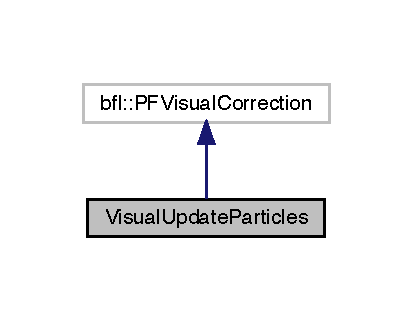
\includegraphics[width=198pt]{classVisualUpdateParticles__inherit__graph}
\end{center}
\end{figure}
\subsection*{Public Member Functions}
\begin{DoxyCompactItemize}
\item 
\hyperlink{classVisualUpdateParticles_aa67179b62e91f386402d176975151d48}{Visual\+Update\+Particles} (std\+::unique\+\_\+ptr$<$ \hyperlink{classVisualProprioception}{Visual\+Proprioception} $>$ observation\+\_\+model) noexcept
\item 
\hyperlink{classVisualUpdateParticles_ade399f29a375d20c3c707dbab2fb23bb}{Visual\+Update\+Particles} (std\+::unique\+\_\+ptr$<$ \hyperlink{classVisualProprioception}{Visual\+Proprioception} $>$ observation\+\_\+model, const double likelihood\+\_\+gain) noexcept
\item 
\hyperlink{classVisualUpdateParticles_a225e07a8873f4ed372b3b12ee4a0f044}{Visual\+Update\+Particles} (std\+::unique\+\_\+ptr$<$ \hyperlink{classVisualProprioception}{Visual\+Proprioception} $>$ observation\+\_\+model, const double likelihood\+\_\+gain, const int num\+\_\+cuda\+\_\+stream) noexcept
\item 
\hyperlink{classVisualUpdateParticles_a96097675396400a8f6932e4c867d9f30}{$\sim$\+Visual\+Update\+Particles} () noexcept
\item 
void \hyperlink{classVisualUpdateParticles_ac6f27c465111a248314ce93ed630dd75}{innovation} (const Eigen\+::\+Ref$<$ const Eigen\+::\+Matrix\+Xf $>$ \&pred\+\_\+states, cv\+::\+Input\+Array measurements, Eigen\+::\+Ref$<$ Eigen\+::\+Matrix\+Xf $>$ innovations) override
\item 
double \hyperlink{classVisualUpdateParticles_ac8905544d7c082cca2fe52b773023bd7}{likelihood} (const Eigen\+::\+Ref$<$ const Eigen\+::\+Matrix\+Xf $>$ \&innovations) override
\item 
bfl\+::\+Visual\+Observation\+Model \& \hyperlink{classVisualUpdateParticles_a34f3b5665eff632890713db818d1995a}{get\+Visual\+Observation\+Model} () override
\item 
void \hyperlink{classVisualUpdateParticles_adced067cb277d138db7f452db1bc01a6}{set\+Visual\+Observation\+Model} (std\+::unique\+\_\+ptr$<$ bfl\+::\+Visual\+Observation\+Model $>$ visual\+\_\+observation\+\_\+model) override
\end{DoxyCompactItemize}
\subsection*{Protected Member Functions}
\begin{DoxyCompactItemize}
\item 
void \hyperlink{classVisualUpdateParticles_ac0ed3c0a2ccab6cbc65a5f83fa834483}{correct\+Step} (const Eigen\+::\+Ref$<$ const Eigen\+::\+Matrix\+Xf $>$ \&pred\+\_\+states, const Eigen\+::\+Ref$<$ const Eigen\+::\+Vector\+Xf $>$ \&pred\+\_\+weights, cv\+::\+Input\+Array measurements, Eigen\+::\+Ref$<$ Eigen\+::\+Matrix\+Xf $>$ cor\+\_\+states, Eigen\+::\+Ref$<$ Eigen\+::\+Vector\+Xf $>$ cor\+\_\+weights) override
\end{DoxyCompactItemize}
\subsection*{Protected Attributes}
\begin{DoxyCompactItemize}
\item 
std\+::unique\+\_\+ptr$<$ \hyperlink{classVisualProprioception}{Visual\+Proprioception} $>$ \hyperlink{classVisualUpdateParticles_a7e076390fd3cb9e508d36d65235b179c}{observation\+\_\+model\+\_\+}
\item 
double \hyperlink{classVisualUpdateParticles_a3199afdf57b24df7193f3f50b87a252f}{likelihood\+\_\+gain\+\_\+}
\item 
cv\+::\+Ptr$<$ cv\+::cuda\+::\+H\+OG $>$ \hyperlink{classVisualUpdateParticles_add09a7f472a034679dfc77726d9cc4c3}{cuda\+\_\+hog\+\_\+}
\item 
const int \hyperlink{classVisualUpdateParticles_ace5e836ecda66975c5ec85ea92c305b8}{num\+\_\+cuda\+\_\+stream\+\_\+}
\item 
const int \hyperlink{classVisualUpdateParticles_aad9d0aba6b913489a8e63f7008ceeebe}{num\+\_\+img\+\_\+stream\+\_\+}
\item 
std\+::vector$<$ cv\+::cuda\+::\+Stream $>$ \hyperlink{classVisualUpdateParticles_af179d2c350a9f93a412200816b79a876}{cuda\+\_\+stream\+\_\+}
\item 
std\+::vector$<$ cv\+::\+Mat $>$ \hyperlink{classVisualUpdateParticles_a61bfe2a44d2cad15887f34484321bd93}{hand\+\_\+rendered\+\_\+}
\item 
std\+::vector$<$ cv\+::cuda\+::\+Gpu\+Mat $>$ \hyperlink{classVisualUpdateParticles_a885d5094c4a20b386607ee839792ce12}{cuda\+\_\+img\+\_\+}
\item 
std\+::vector$<$ cv\+::cuda\+::\+Gpu\+Mat $>$ \hyperlink{classVisualUpdateParticles_acb31efd3272b83b80e55018e577adbfc}{cuda\+\_\+img\+\_\+alpha\+\_\+}
\item 
std\+::vector$<$ cv\+::cuda\+::\+Gpu\+Mat $>$ \hyperlink{classVisualUpdateParticles_ae2de27efd67d8c5cfa661d97841aa9ea}{cuda\+\_\+descriptors\+\_\+}
\item 
std\+::vector$<$ cv\+::\+Mat $>$ \hyperlink{classVisualUpdateParticles_ac9c29a18fee44cd0bb5be0ff71e2f8d7}{cpu\+\_\+descriptors\+\_\+}
\end{DoxyCompactItemize}


\subsection{Detailed Description}


Definition at line 16 of file Visual\+Update\+Particles.\+h.



\subsection{Constructor \& Destructor Documentation}
\mbox{\Hypertarget{classVisualUpdateParticles_aa67179b62e91f386402d176975151d48}\label{classVisualUpdateParticles_aa67179b62e91f386402d176975151d48}} 
\index{Visual\+Update\+Particles@{Visual\+Update\+Particles}!Visual\+Update\+Particles@{Visual\+Update\+Particles}}
\index{Visual\+Update\+Particles@{Visual\+Update\+Particles}!Visual\+Update\+Particles@{Visual\+Update\+Particles}}
\subsubsection{\texorpdfstring{Visual\+Update\+Particles()}{VisualUpdateParticles()}\hspace{0.1cm}{\footnotesize\ttfamily [1/3]}}
{\footnotesize\ttfamily Visual\+Update\+Particles\+::\+Visual\+Update\+Particles (\begin{DoxyParamCaption}\item[{std\+::unique\+\_\+ptr$<$ \hyperlink{classVisualProprioception}{Visual\+Proprioception} $>$}]{observation\+\_\+model }\end{DoxyParamCaption})\hspace{0.3cm}{\ttfamily [noexcept]}}



Definition at line 21 of file Visual\+Update\+Particles.\+cpp.

\mbox{\Hypertarget{classVisualUpdateParticles_ade399f29a375d20c3c707dbab2fb23bb}\label{classVisualUpdateParticles_ade399f29a375d20c3c707dbab2fb23bb}} 
\index{Visual\+Update\+Particles@{Visual\+Update\+Particles}!Visual\+Update\+Particles@{Visual\+Update\+Particles}}
\index{Visual\+Update\+Particles@{Visual\+Update\+Particles}!Visual\+Update\+Particles@{Visual\+Update\+Particles}}
\subsubsection{\texorpdfstring{Visual\+Update\+Particles()}{VisualUpdateParticles()}\hspace{0.1cm}{\footnotesize\ttfamily [2/3]}}
{\footnotesize\ttfamily Visual\+Update\+Particles\+::\+Visual\+Update\+Particles (\begin{DoxyParamCaption}\item[{std\+::unique\+\_\+ptr$<$ \hyperlink{classVisualProprioception}{Visual\+Proprioception} $>$}]{observation\+\_\+model,  }\item[{const double}]{likelihood\+\_\+gain }\end{DoxyParamCaption})\hspace{0.3cm}{\ttfamily [noexcept]}}



Definition at line 25 of file Visual\+Update\+Particles.\+cpp.

\mbox{\Hypertarget{classVisualUpdateParticles_a225e07a8873f4ed372b3b12ee4a0f044}\label{classVisualUpdateParticles_a225e07a8873f4ed372b3b12ee4a0f044}} 
\index{Visual\+Update\+Particles@{Visual\+Update\+Particles}!Visual\+Update\+Particles@{Visual\+Update\+Particles}}
\index{Visual\+Update\+Particles@{Visual\+Update\+Particles}!Visual\+Update\+Particles@{Visual\+Update\+Particles}}
\subsubsection{\texorpdfstring{Visual\+Update\+Particles()}{VisualUpdateParticles()}\hspace{0.1cm}{\footnotesize\ttfamily [3/3]}}
{\footnotesize\ttfamily Visual\+Update\+Particles\+::\+Visual\+Update\+Particles (\begin{DoxyParamCaption}\item[{std\+::unique\+\_\+ptr$<$ \hyperlink{classVisualProprioception}{Visual\+Proprioception} $>$}]{observation\+\_\+model,  }\item[{const double}]{likelihood\+\_\+gain,  }\item[{const int}]{num\+\_\+cuda\+\_\+stream }\end{DoxyParamCaption})\hspace{0.3cm}{\ttfamily [noexcept]}}



Definition at line 29 of file Visual\+Update\+Particles.\+cpp.

\mbox{\Hypertarget{classVisualUpdateParticles_a96097675396400a8f6932e4c867d9f30}\label{classVisualUpdateParticles_a96097675396400a8f6932e4c867d9f30}} 
\index{Visual\+Update\+Particles@{Visual\+Update\+Particles}!````~Visual\+Update\+Particles@{$\sim$\+Visual\+Update\+Particles}}
\index{````~Visual\+Update\+Particles@{$\sim$\+Visual\+Update\+Particles}!Visual\+Update\+Particles@{Visual\+Update\+Particles}}
\subsubsection{\texorpdfstring{$\sim$\+Visual\+Update\+Particles()}{~VisualUpdateParticles()}}
{\footnotesize\ttfamily Visual\+Update\+Particles\+::$\sim$\+Visual\+Update\+Particles (\begin{DoxyParamCaption}{ }\end{DoxyParamCaption})\hspace{0.3cm}{\ttfamily [noexcept]}}



Definition at line 60 of file Visual\+Update\+Particles.\+cpp.



\subsection{Member Function Documentation}
\mbox{\Hypertarget{classVisualUpdateParticles_ac0ed3c0a2ccab6cbc65a5f83fa834483}\label{classVisualUpdateParticles_ac0ed3c0a2ccab6cbc65a5f83fa834483}} 
\index{Visual\+Update\+Particles@{Visual\+Update\+Particles}!correct\+Step@{correct\+Step}}
\index{correct\+Step@{correct\+Step}!Visual\+Update\+Particles@{Visual\+Update\+Particles}}
\subsubsection{\texorpdfstring{correct\+Step()}{correctStep()}}
{\footnotesize\ttfamily void Visual\+Update\+Particles\+::correct\+Step (\begin{DoxyParamCaption}\item[{const Eigen\+::\+Ref$<$ const Eigen\+::\+Matrix\+Xf $>$ \&}]{pred\+\_\+states,  }\item[{const Eigen\+::\+Ref$<$ const Eigen\+::\+Vector\+Xf $>$ \&}]{pred\+\_\+weights,  }\item[{cv\+::\+Input\+Array}]{measurements,  }\item[{Eigen\+::\+Ref$<$ Eigen\+::\+Matrix\+Xf $>$}]{cor\+\_\+states,  }\item[{Eigen\+::\+Ref$<$ Eigen\+::\+Vector\+Xf $>$}]{cor\+\_\+weights }\end{DoxyParamCaption})\hspace{0.3cm}{\ttfamily [override]}, {\ttfamily [protected]}}



Definition at line 125 of file Visual\+Update\+Particles.\+cpp.

\mbox{\Hypertarget{classVisualUpdateParticles_a34f3b5665eff632890713db818d1995a}\label{classVisualUpdateParticles_a34f3b5665eff632890713db818d1995a}} 
\index{Visual\+Update\+Particles@{Visual\+Update\+Particles}!get\+Visual\+Observation\+Model@{get\+Visual\+Observation\+Model}}
\index{get\+Visual\+Observation\+Model@{get\+Visual\+Observation\+Model}!Visual\+Update\+Particles@{Visual\+Update\+Particles}}
\subsubsection{\texorpdfstring{get\+Visual\+Observation\+Model()}{getVisualObservationModel()}}
{\footnotesize\ttfamily bfl\+::\+Visual\+Observation\+Model \& Visual\+Update\+Particles\+::get\+Visual\+Observation\+Model (\begin{DoxyParamCaption}{ }\end{DoxyParamCaption})\hspace{0.3cm}{\ttfamily [override]}}



Definition at line 109 of file Visual\+Update\+Particles.\+cpp.

\mbox{\Hypertarget{classVisualUpdateParticles_ac6f27c465111a248314ce93ed630dd75}\label{classVisualUpdateParticles_ac6f27c465111a248314ce93ed630dd75}} 
\index{Visual\+Update\+Particles@{Visual\+Update\+Particles}!innovation@{innovation}}
\index{innovation@{innovation}!Visual\+Update\+Particles@{Visual\+Update\+Particles}}
\subsubsection{\texorpdfstring{innovation()}{innovation()}}
{\footnotesize\ttfamily void Visual\+Update\+Particles\+::innovation (\begin{DoxyParamCaption}\item[{const Eigen\+::\+Ref$<$ const Eigen\+::\+Matrix\+Xf $>$ \&}]{pred\+\_\+states,  }\item[{cv\+::\+Input\+Array}]{measurements,  }\item[{Eigen\+::\+Ref$<$ Eigen\+::\+Matrix\+Xf $>$}]{innovations }\end{DoxyParamCaption})\hspace{0.3cm}{\ttfamily [override]}}



Definition at line 63 of file Visual\+Update\+Particles.\+cpp.

\mbox{\Hypertarget{classVisualUpdateParticles_ac8905544d7c082cca2fe52b773023bd7}\label{classVisualUpdateParticles_ac8905544d7c082cca2fe52b773023bd7}} 
\index{Visual\+Update\+Particles@{Visual\+Update\+Particles}!likelihood@{likelihood}}
\index{likelihood@{likelihood}!Visual\+Update\+Particles@{Visual\+Update\+Particles}}
\subsubsection{\texorpdfstring{likelihood()}{likelihood()}}
{\footnotesize\ttfamily double Visual\+Update\+Particles\+::likelihood (\begin{DoxyParamCaption}\item[{const Eigen\+::\+Ref$<$ const Eigen\+::\+Matrix\+Xf $>$ \&}]{innovations }\end{DoxyParamCaption})\hspace{0.3cm}{\ttfamily [override]}}



Definition at line 103 of file Visual\+Update\+Particles.\+cpp.

\mbox{\Hypertarget{classVisualUpdateParticles_adced067cb277d138db7f452db1bc01a6}\label{classVisualUpdateParticles_adced067cb277d138db7f452db1bc01a6}} 
\index{Visual\+Update\+Particles@{Visual\+Update\+Particles}!set\+Visual\+Observation\+Model@{set\+Visual\+Observation\+Model}}
\index{set\+Visual\+Observation\+Model@{set\+Visual\+Observation\+Model}!Visual\+Update\+Particles@{Visual\+Update\+Particles}}
\subsubsection{\texorpdfstring{set\+Visual\+Observation\+Model()}{setVisualObservationModel()}}
{\footnotesize\ttfamily void Visual\+Update\+Particles\+::set\+Visual\+Observation\+Model (\begin{DoxyParamCaption}\item[{std\+::unique\+\_\+ptr$<$ bfl\+::\+Visual\+Observation\+Model $>$}]{visual\+\_\+observation\+\_\+model }\end{DoxyParamCaption})\hspace{0.3cm}{\ttfamily [override]}}



Definition at line 115 of file Visual\+Update\+Particles.\+cpp.



\subsection{Member Data Documentation}
\mbox{\Hypertarget{classVisualUpdateParticles_ac9c29a18fee44cd0bb5be0ff71e2f8d7}\label{classVisualUpdateParticles_ac9c29a18fee44cd0bb5be0ff71e2f8d7}} 
\index{Visual\+Update\+Particles@{Visual\+Update\+Particles}!cpu\+\_\+descriptors\+\_\+@{cpu\+\_\+descriptors\+\_\+}}
\index{cpu\+\_\+descriptors\+\_\+@{cpu\+\_\+descriptors\+\_\+}!Visual\+Update\+Particles@{Visual\+Update\+Particles}}
\subsubsection{\texorpdfstring{cpu\+\_\+descriptors\+\_\+}{cpu\_descriptors\_}}
{\footnotesize\ttfamily std\+::vector$<$cv\+::\+Mat$>$ Visual\+Update\+Particles\+::cpu\+\_\+descriptors\+\_\+\hspace{0.3cm}{\ttfamily [protected]}}



Definition at line 51 of file Visual\+Update\+Particles.\+h.

\mbox{\Hypertarget{classVisualUpdateParticles_ae2de27efd67d8c5cfa661d97841aa9ea}\label{classVisualUpdateParticles_ae2de27efd67d8c5cfa661d97841aa9ea}} 
\index{Visual\+Update\+Particles@{Visual\+Update\+Particles}!cuda\+\_\+descriptors\+\_\+@{cuda\+\_\+descriptors\+\_\+}}
\index{cuda\+\_\+descriptors\+\_\+@{cuda\+\_\+descriptors\+\_\+}!Visual\+Update\+Particles@{Visual\+Update\+Particles}}
\subsubsection{\texorpdfstring{cuda\+\_\+descriptors\+\_\+}{cuda\_descriptors\_}}
{\footnotesize\ttfamily std\+::vector$<$cv\+::cuda\+::\+Gpu\+Mat$>$ Visual\+Update\+Particles\+::cuda\+\_\+descriptors\+\_\+\hspace{0.3cm}{\ttfamily [protected]}}



Definition at line 50 of file Visual\+Update\+Particles.\+h.

\mbox{\Hypertarget{classVisualUpdateParticles_add09a7f472a034679dfc77726d9cc4c3}\label{classVisualUpdateParticles_add09a7f472a034679dfc77726d9cc4c3}} 
\index{Visual\+Update\+Particles@{Visual\+Update\+Particles}!cuda\+\_\+hog\+\_\+@{cuda\+\_\+hog\+\_\+}}
\index{cuda\+\_\+hog\+\_\+@{cuda\+\_\+hog\+\_\+}!Visual\+Update\+Particles@{Visual\+Update\+Particles}}
\subsubsection{\texorpdfstring{cuda\+\_\+hog\+\_\+}{cuda\_hog\_}}
{\footnotesize\ttfamily cv\+::\+Ptr$<$cv\+::cuda\+::\+H\+OG$>$ Visual\+Update\+Particles\+::cuda\+\_\+hog\+\_\+\hspace{0.3cm}{\ttfamily [protected]}}



Definition at line 42 of file Visual\+Update\+Particles.\+h.

\mbox{\Hypertarget{classVisualUpdateParticles_a885d5094c4a20b386607ee839792ce12}\label{classVisualUpdateParticles_a885d5094c4a20b386607ee839792ce12}} 
\index{Visual\+Update\+Particles@{Visual\+Update\+Particles}!cuda\+\_\+img\+\_\+@{cuda\+\_\+img\+\_\+}}
\index{cuda\+\_\+img\+\_\+@{cuda\+\_\+img\+\_\+}!Visual\+Update\+Particles@{Visual\+Update\+Particles}}
\subsubsection{\texorpdfstring{cuda\+\_\+img\+\_\+}{cuda\_img\_}}
{\footnotesize\ttfamily std\+::vector$<$cv\+::cuda\+::\+Gpu\+Mat$>$ Visual\+Update\+Particles\+::cuda\+\_\+img\+\_\+\hspace{0.3cm}{\ttfamily [protected]}}



Definition at line 48 of file Visual\+Update\+Particles.\+h.

\mbox{\Hypertarget{classVisualUpdateParticles_acb31efd3272b83b80e55018e577adbfc}\label{classVisualUpdateParticles_acb31efd3272b83b80e55018e577adbfc}} 
\index{Visual\+Update\+Particles@{Visual\+Update\+Particles}!cuda\+\_\+img\+\_\+alpha\+\_\+@{cuda\+\_\+img\+\_\+alpha\+\_\+}}
\index{cuda\+\_\+img\+\_\+alpha\+\_\+@{cuda\+\_\+img\+\_\+alpha\+\_\+}!Visual\+Update\+Particles@{Visual\+Update\+Particles}}
\subsubsection{\texorpdfstring{cuda\+\_\+img\+\_\+alpha\+\_\+}{cuda\_img\_alpha\_}}
{\footnotesize\ttfamily std\+::vector$<$cv\+::cuda\+::\+Gpu\+Mat$>$ Visual\+Update\+Particles\+::cuda\+\_\+img\+\_\+alpha\+\_\+\hspace{0.3cm}{\ttfamily [protected]}}



Definition at line 49 of file Visual\+Update\+Particles.\+h.

\mbox{\Hypertarget{classVisualUpdateParticles_af179d2c350a9f93a412200816b79a876}\label{classVisualUpdateParticles_af179d2c350a9f93a412200816b79a876}} 
\index{Visual\+Update\+Particles@{Visual\+Update\+Particles}!cuda\+\_\+stream\+\_\+@{cuda\+\_\+stream\+\_\+}}
\index{cuda\+\_\+stream\+\_\+@{cuda\+\_\+stream\+\_\+}!Visual\+Update\+Particles@{Visual\+Update\+Particles}}
\subsubsection{\texorpdfstring{cuda\+\_\+stream\+\_\+}{cuda\_stream\_}}
{\footnotesize\ttfamily std\+::vector$<$cv\+::cuda\+::\+Stream$>$ Visual\+Update\+Particles\+::cuda\+\_\+stream\+\_\+\hspace{0.3cm}{\ttfamily [protected]}}



Definition at line 46 of file Visual\+Update\+Particles.\+h.

\mbox{\Hypertarget{classVisualUpdateParticles_a61bfe2a44d2cad15887f34484321bd93}\label{classVisualUpdateParticles_a61bfe2a44d2cad15887f34484321bd93}} 
\index{Visual\+Update\+Particles@{Visual\+Update\+Particles}!hand\+\_\+rendered\+\_\+@{hand\+\_\+rendered\+\_\+}}
\index{hand\+\_\+rendered\+\_\+@{hand\+\_\+rendered\+\_\+}!Visual\+Update\+Particles@{Visual\+Update\+Particles}}
\subsubsection{\texorpdfstring{hand\+\_\+rendered\+\_\+}{hand\_rendered\_}}
{\footnotesize\ttfamily std\+::vector$<$cv\+::\+Mat$>$ Visual\+Update\+Particles\+::hand\+\_\+rendered\+\_\+\hspace{0.3cm}{\ttfamily [protected]}}



Definition at line 47 of file Visual\+Update\+Particles.\+h.

\mbox{\Hypertarget{classVisualUpdateParticles_a3199afdf57b24df7193f3f50b87a252f}\label{classVisualUpdateParticles_a3199afdf57b24df7193f3f50b87a252f}} 
\index{Visual\+Update\+Particles@{Visual\+Update\+Particles}!likelihood\+\_\+gain\+\_\+@{likelihood\+\_\+gain\+\_\+}}
\index{likelihood\+\_\+gain\+\_\+@{likelihood\+\_\+gain\+\_\+}!Visual\+Update\+Particles@{Visual\+Update\+Particles}}
\subsubsection{\texorpdfstring{likelihood\+\_\+gain\+\_\+}{likelihood\_gain\_}}
{\footnotesize\ttfamily double Visual\+Update\+Particles\+::likelihood\+\_\+gain\+\_\+\hspace{0.3cm}{\ttfamily [protected]}}



Definition at line 40 of file Visual\+Update\+Particles.\+h.

\mbox{\Hypertarget{classVisualUpdateParticles_ace5e836ecda66975c5ec85ea92c305b8}\label{classVisualUpdateParticles_ace5e836ecda66975c5ec85ea92c305b8}} 
\index{Visual\+Update\+Particles@{Visual\+Update\+Particles}!num\+\_\+cuda\+\_\+stream\+\_\+@{num\+\_\+cuda\+\_\+stream\+\_\+}}
\index{num\+\_\+cuda\+\_\+stream\+\_\+@{num\+\_\+cuda\+\_\+stream\+\_\+}!Visual\+Update\+Particles@{Visual\+Update\+Particles}}
\subsubsection{\texorpdfstring{num\+\_\+cuda\+\_\+stream\+\_\+}{num\_cuda\_stream\_}}
{\footnotesize\ttfamily const int Visual\+Update\+Particles\+::num\+\_\+cuda\+\_\+stream\+\_\+\hspace{0.3cm}{\ttfamily [protected]}}



Definition at line 44 of file Visual\+Update\+Particles.\+h.

\mbox{\Hypertarget{classVisualUpdateParticles_aad9d0aba6b913489a8e63f7008ceeebe}\label{classVisualUpdateParticles_aad9d0aba6b913489a8e63f7008ceeebe}} 
\index{Visual\+Update\+Particles@{Visual\+Update\+Particles}!num\+\_\+img\+\_\+stream\+\_\+@{num\+\_\+img\+\_\+stream\+\_\+}}
\index{num\+\_\+img\+\_\+stream\+\_\+@{num\+\_\+img\+\_\+stream\+\_\+}!Visual\+Update\+Particles@{Visual\+Update\+Particles}}
\subsubsection{\texorpdfstring{num\+\_\+img\+\_\+stream\+\_\+}{num\_img\_stream\_}}
{\footnotesize\ttfamily const int Visual\+Update\+Particles\+::num\+\_\+img\+\_\+stream\+\_\+\hspace{0.3cm}{\ttfamily [protected]}}



Definition at line 45 of file Visual\+Update\+Particles.\+h.

\mbox{\Hypertarget{classVisualUpdateParticles_a7e076390fd3cb9e508d36d65235b179c}\label{classVisualUpdateParticles_a7e076390fd3cb9e508d36d65235b179c}} 
\index{Visual\+Update\+Particles@{Visual\+Update\+Particles}!observation\+\_\+model\+\_\+@{observation\+\_\+model\+\_\+}}
\index{observation\+\_\+model\+\_\+@{observation\+\_\+model\+\_\+}!Visual\+Update\+Particles@{Visual\+Update\+Particles}}
\subsubsection{\texorpdfstring{observation\+\_\+model\+\_\+}{observation\_model\_}}
{\footnotesize\ttfamily std\+::unique\+\_\+ptr$<$\hyperlink{classVisualProprioception}{Visual\+Proprioception}$>$ Visual\+Update\+Particles\+::observation\+\_\+model\+\_\+\hspace{0.3cm}{\ttfamily [protected]}}



Definition at line 39 of file Visual\+Update\+Particles.\+h.



The documentation for this class was generated from the following files\+:\begin{DoxyCompactItemize}
\item 
/\+Users/\+Claudio/\+Git\+Hub/visual-\/tracking-\/control/src/hand-\/tracking/include/\hyperlink{VisualUpdateParticles_8h}{Visual\+Update\+Particles.\+h}\item 
/\+Users/\+Claudio/\+Git\+Hub/visual-\/tracking-\/control/src/hand-\/tracking/src/\hyperlink{VisualUpdateParticles_8cpp}{Visual\+Update\+Particles.\+cpp}\end{DoxyCompactItemize}

\chapter{File Documentation}
\hypertarget{hand-tracking_8dox}{}\section{generated-\/from-\/xml/hand-\/tracking.dox File Reference}
\label{hand-tracking_8dox}\index{generated-\/from-\/xml/hand-\/tracking.\+dox@{generated-\/from-\/xml/hand-\/tracking.\+dox}}

\hypertarget{visualservoingclient_8dox}{}\section{generated-\/from-\/xml/visualservoingclient.dox File Reference}
\label{visualservoingclient_8dox}\index{generated-\/from-\/xml/visualservoingclient.\+dox@{generated-\/from-\/xml/visualservoingclient.\+dox}}

\hypertarget{visualservoingserver_8dox}{}\section{generated-\/from-\/xml/visualservoingserver.dox File Reference}
\label{visualservoingserver_8dox}\index{generated-\/from-\/xml/visualservoingserver.\+dox@{generated-\/from-\/xml/visualservoingserver.\+dox}}

\hypertarget{VisualServoingIDL_8h}{}\section{idl\+\_\+dox/\+Visual\+Servoing\+I\+DL.h File Reference}
\label{VisualServoingIDL_8h}\index{idl\+\_\+dox/\+Visual\+Servoing\+I\+D\+L.\+h@{idl\+\_\+dox/\+Visual\+Servoing\+I\+D\+L.\+h}}
{\ttfamily \#include $<$yarp/os/\+Wire.\+h$>$}\newline
{\ttfamily \#include $<$yarp/os/idl/\+Wire\+Types.\+h$>$}\newline
Include dependency graph for Visual\+Servoing\+I\+D\+L.\+h\+:
\nopagebreak
\begin{figure}[H]
\begin{center}
\leavevmode
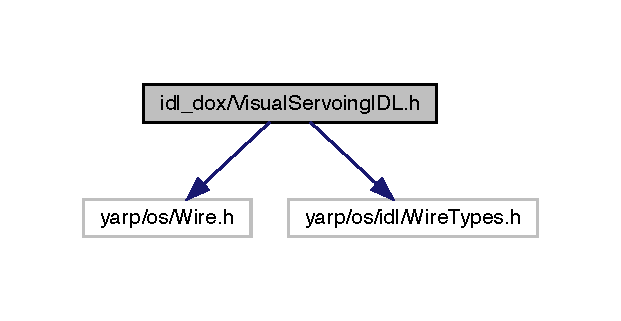
\includegraphics[width=298pt]{VisualServoingIDL_8h__incl}
\end{center}
\end{figure}
\subsection*{Classes}
\begin{DoxyCompactItemize}
\item 
class \hyperlink{classVisualServoingIDL}{Visual\+Servoing\+I\+DL}
\begin{DoxyCompactList}\small\item\em \hyperlink{classVisualServoingIDL}{Visual\+Servoing\+I\+DL} I\+DL Interface to Server\+Visual\+Servoing functionalities. \end{DoxyCompactList}\end{DoxyCompactItemize}

\hypertarget{VisualSISParticleFilterIDL_8h}{}\section{idl\+\_\+dox/\+Visual\+S\+I\+S\+Particle\+Filter\+I\+DL.h File Reference}
\label{VisualSISParticleFilterIDL_8h}\index{idl\+\_\+dox/\+Visual\+S\+I\+S\+Particle\+Filter\+I\+D\+L.\+h@{idl\+\_\+dox/\+Visual\+S\+I\+S\+Particle\+Filter\+I\+D\+L.\+h}}
{\ttfamily \#include $<$yarp/os/\+Wire.\+h$>$}\newline
{\ttfamily \#include $<$yarp/os/idl/\+Wire\+Types.\+h$>$}\newline
Include dependency graph for Visual\+S\+I\+S\+Particle\+Filter\+I\+D\+L.\+h\+:
\nopagebreak
\begin{figure}[H]
\begin{center}
\leavevmode
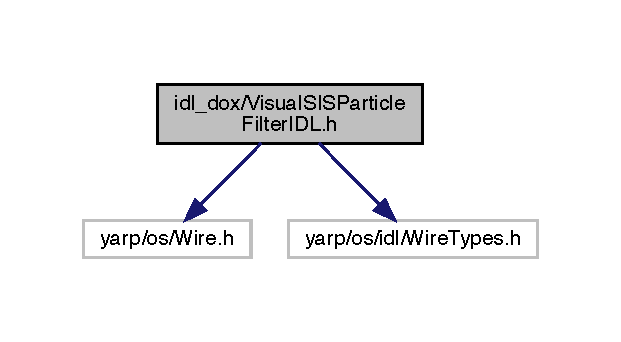
\includegraphics[width=298pt]{VisualSISParticleFilterIDL_8h__incl}
\end{center}
\end{figure}
\subsection*{Classes}
\begin{DoxyCompactItemize}
\item 
class \hyperlink{classVisualSISParticleFilterIDL}{Visual\+S\+I\+S\+Particle\+Filter\+I\+DL}
\begin{DoxyCompactList}\small\item\em \hyperlink{classVisualSISParticleFilterIDL}{Visual\+S\+I\+S\+Particle\+Filter\+I\+DL} I\+DL Interface to Visual\+S\+I\+R\+Particle\+Filter options. \end{DoxyCompactList}\end{DoxyCompactItemize}

\hypertarget{mainpage_8md}{}\section{mainpage.\+md File Reference}
\label{mainpage_8md}\index{mainpage.\+md@{mainpage.\+md}}

\hypertarget{BrownianMotionPose_8h}{}\section{/\+Users/\+Claudio/\+Git\+Hub/visual-\/tracking-\/control/src/hand-\/tracking/include/\+Brownian\+Motion\+Pose.h File Reference}
\label{BrownianMotionPose_8h}\index{/\+Users/\+Claudio/\+Git\+Hub/visual-\/tracking-\/control/src/hand-\/tracking/include/\+Brownian\+Motion\+Pose.\+h@{/\+Users/\+Claudio/\+Git\+Hub/visual-\/tracking-\/control/src/hand-\/tracking/include/\+Brownian\+Motion\+Pose.\+h}}
{\ttfamily \#include $<$functional$>$}\newline
{\ttfamily \#include $<$random$>$}\newline
{\ttfamily \#include $<$Bayes\+Filters/\+State\+Model.\+h$>$}\newline
Include dependency graph for Brownian\+Motion\+Pose.\+h\+:
\nopagebreak
\begin{figure}[H]
\begin{center}
\leavevmode
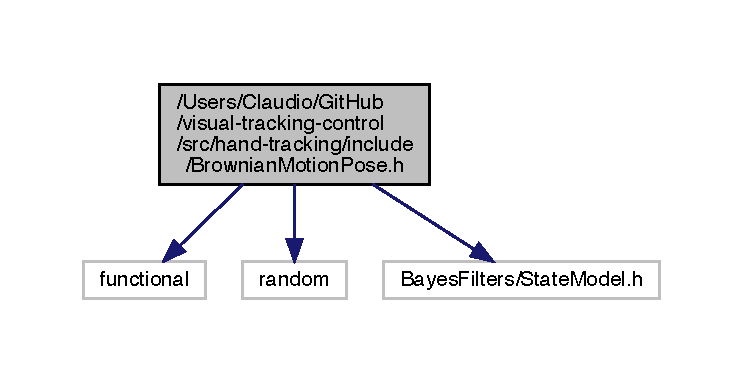
\includegraphics[width=350pt]{BrownianMotionPose_8h__incl}
\end{center}
\end{figure}
This graph shows which files directly or indirectly include this file\+:
\nopagebreak
\begin{figure}[H]
\begin{center}
\leavevmode
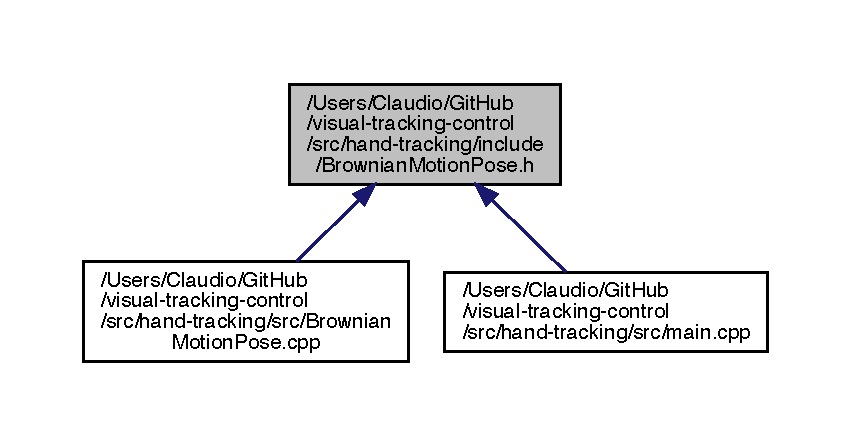
\includegraphics[width=350pt]{BrownianMotionPose_8h__dep__incl}
\end{center}
\end{figure}
\subsection*{Classes}
\begin{DoxyCompactItemize}
\item 
class \hyperlink{classBrownianMotionPose}{Brownian\+Motion\+Pose}
\end{DoxyCompactItemize}

\hypertarget{DrawFwdKinPoses_8h}{}\section{/\+Users/\+Claudio/\+Git\+Hub/visual-\/tracking-\/control/src/hand-\/tracking/include/\+Draw\+Fwd\+Kin\+Poses.h File Reference}
\label{DrawFwdKinPoses_8h}\index{/\+Users/\+Claudio/\+Git\+Hub/visual-\/tracking-\/control/src/hand-\/tracking/include/\+Draw\+Fwd\+Kin\+Poses.\+h@{/\+Users/\+Claudio/\+Git\+Hub/visual-\/tracking-\/control/src/hand-\/tracking/include/\+Draw\+Fwd\+Kin\+Poses.\+h}}
{\ttfamily \#include $<$memory$>$}\newline
{\ttfamily \#include $<$random$>$}\newline
{\ttfamily \#include $<$Bayes\+Filters/\+P\+F\+Prediction.\+h$>$}\newline
{\ttfamily \#include $<$Bayes\+Filters/\+State\+Model.\+h$>$}\newline
Include dependency graph for Draw\+Fwd\+Kin\+Poses.\+h\+:
\nopagebreak
\begin{figure}[H]
\begin{center}
\leavevmode
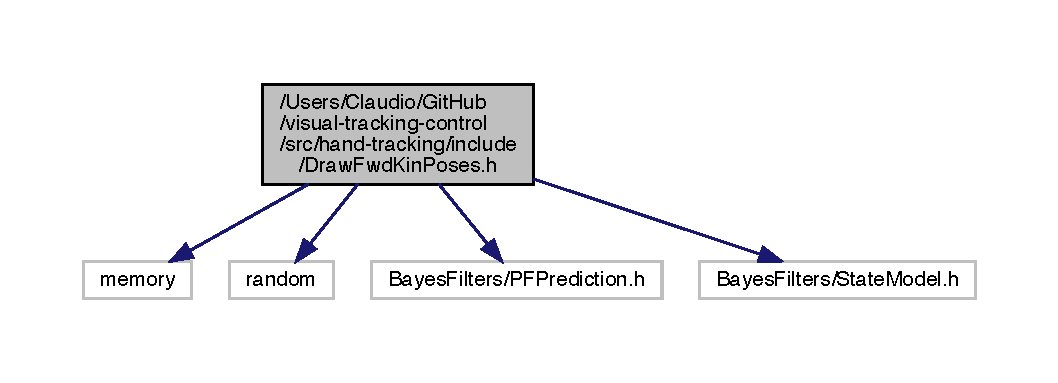
\includegraphics[width=350pt]{DrawFwdKinPoses_8h__incl}
\end{center}
\end{figure}
This graph shows which files directly or indirectly include this file\+:
\nopagebreak
\begin{figure}[H]
\begin{center}
\leavevmode
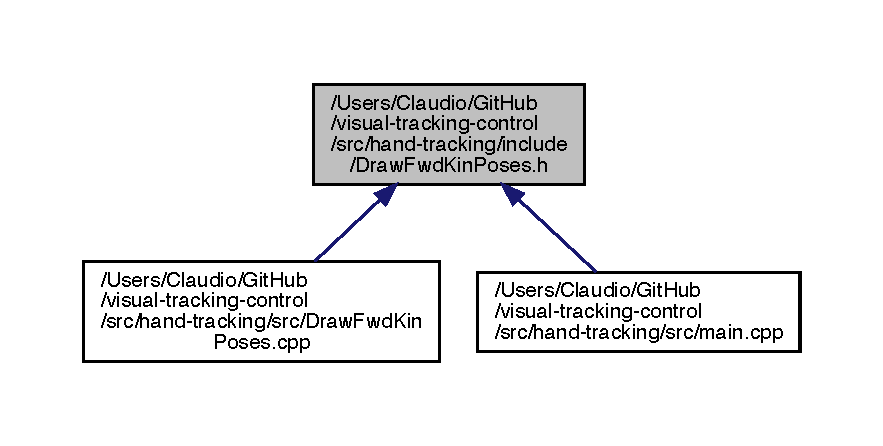
\includegraphics[width=350pt]{DrawFwdKinPoses_8h__dep__incl}
\end{center}
\end{figure}
\subsection*{Classes}
\begin{DoxyCompactItemize}
\item 
class \hyperlink{classbfl_1_1DrawFwdKinPoses}{bfl\+::\+Draw\+Fwd\+Kin\+Poses}
\end{DoxyCompactItemize}
\subsection*{Namespaces}
\begin{DoxyCompactItemize}
\item 
 \hyperlink{namespacebfl}{bfl}
\end{DoxyCompactItemize}

\hypertarget{FwdKinModel_8h}{}\section{/\+Users/\+Claudio/\+Git\+Hub/visual-\/tracking-\/control/src/hand-\/tracking/include/\+Fwd\+Kin\+Model.h File Reference}
\label{FwdKinModel_8h}\index{/\+Users/\+Claudio/\+Git\+Hub/visual-\/tracking-\/control/src/hand-\/tracking/include/\+Fwd\+Kin\+Model.\+h@{/\+Users/\+Claudio/\+Git\+Hub/visual-\/tracking-\/control/src/hand-\/tracking/include/\+Fwd\+Kin\+Model.\+h}}
{\ttfamily \#include $<$Bayes\+Filters/\+Exogenous\+Model.\+h$>$}\newline
{\ttfamily \#include $<$i\+Cub/i\+Kin/i\+Kin\+Fwd.\+h$>$}\newline
{\ttfamily \#include $<$yarp/dev/\+Poly\+Driver.\+h$>$}\newline
{\ttfamily \#include $<$yarp/dev/\+I\+Encoders.\+h$>$}\newline
{\ttfamily \#include $<$yarp/os/\+Const\+String.\+h$>$}\newline
{\ttfamily \#include $<$yarp/sig/\+Vector.\+h$>$}\newline
Include dependency graph for Fwd\+Kin\+Model.\+h\+:
\nopagebreak
\begin{figure}[H]
\begin{center}
\leavevmode
\includegraphics[width=350pt]{FwdKinModel_8h__incl}
\end{center}
\end{figure}
This graph shows which files directly or indirectly include this file\+:
\nopagebreak
\begin{figure}[H]
\begin{center}
\leavevmode
\includegraphics[width=350pt]{FwdKinModel_8h__dep__incl}
\end{center}
\end{figure}
\subsection*{Classes}
\begin{DoxyCompactItemize}
\item 
class \hyperlink{classFwdKinModel}{Fwd\+Kin\+Model}
\end{DoxyCompactItemize}

\hypertarget{GatePose_8h}{}\section{/\+Users/\+Claudio/\+Git\+Hub/visual-\/tracking-\/control/src/hand-\/tracking/include/\+Gate\+Pose.h File Reference}
\label{GatePose_8h}\index{/\+Users/\+Claudio/\+Git\+Hub/visual-\/tracking-\/control/src/hand-\/tracking/include/\+Gate\+Pose.\+h@{/\+Users/\+Claudio/\+Git\+Hub/visual-\/tracking-\/control/src/hand-\/tracking/include/\+Gate\+Pose.\+h}}
{\ttfamily \#include $<$string$>$}\newline
{\ttfamily \#include $<$Bayes\+Filters/\+P\+F\+Visual\+Correction\+Decorator.\+h$>$}\newline
{\ttfamily \#include $<$Bayes\+Filters/\+State\+Model.\+h$>$}\newline
Include dependency graph for Gate\+Pose.\+h\+:
\nopagebreak
\begin{figure}[H]
\begin{center}
\leavevmode
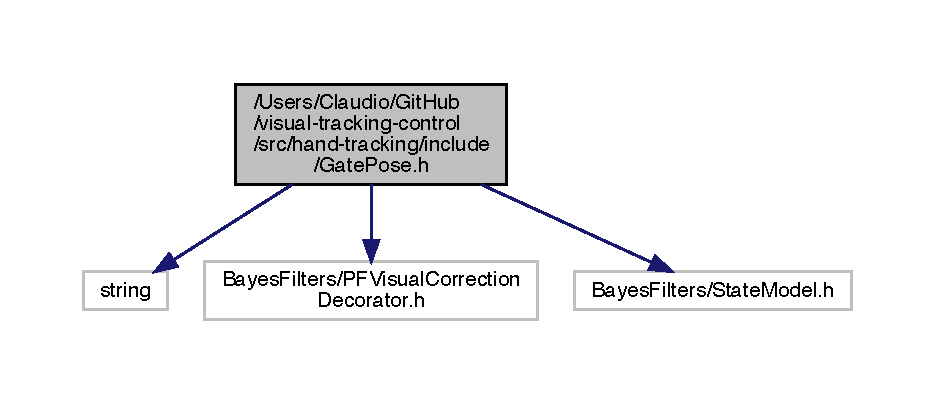
\includegraphics[width=350pt]{GatePose_8h__incl}
\end{center}
\end{figure}
This graph shows which files directly or indirectly include this file\+:
\nopagebreak
\begin{figure}[H]
\begin{center}
\leavevmode
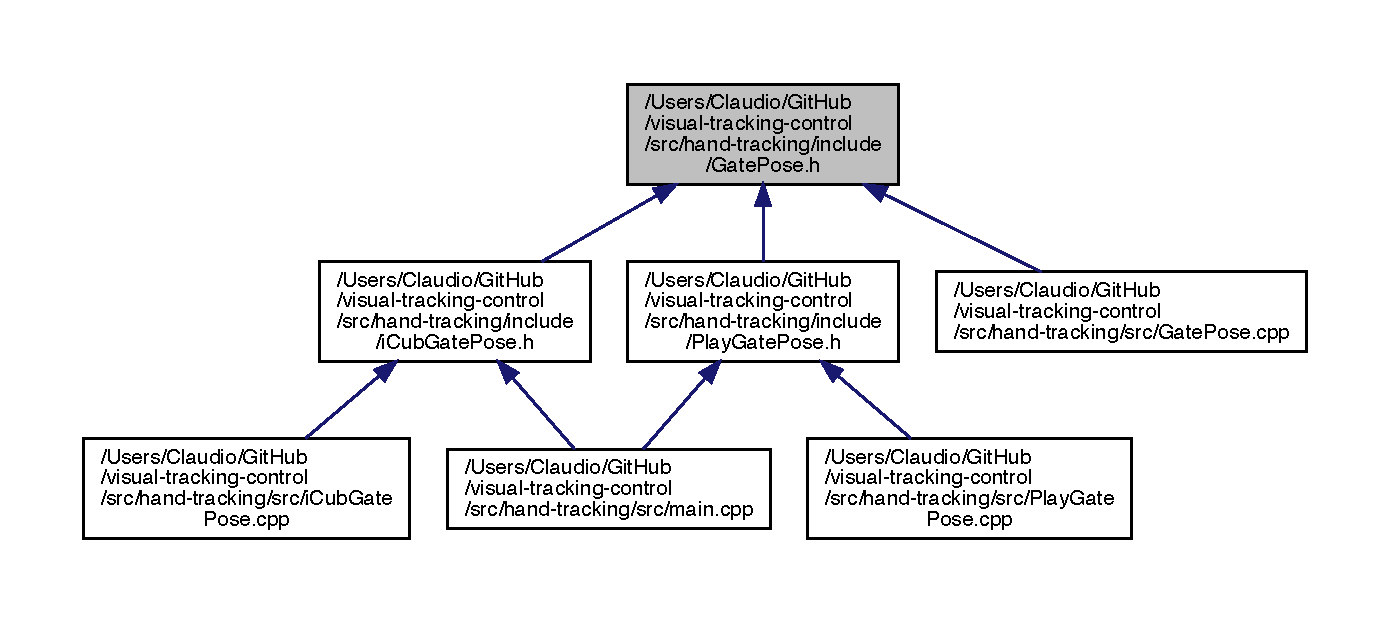
\includegraphics[width=350pt]{GatePose_8h__dep__incl}
\end{center}
\end{figure}
\subsection*{Classes}
\begin{DoxyCompactItemize}
\item 
class \hyperlink{classGatePose}{Gate\+Pose}
\end{DoxyCompactItemize}

\hypertarget{iCubFwdKinModel_8h}{}\section{/\+Users/\+Claudio/\+Git\+Hub/visual-\/tracking-\/control/src/hand-\/tracking/include/i\+Cub\+Fwd\+Kin\+Model.h File Reference}
\label{iCubFwdKinModel_8h}\index{/\+Users/\+Claudio/\+Git\+Hub/visual-\/tracking-\/control/src/hand-\/tracking/include/i\+Cub\+Fwd\+Kin\+Model.\+h@{/\+Users/\+Claudio/\+Git\+Hub/visual-\/tracking-\/control/src/hand-\/tracking/include/i\+Cub\+Fwd\+Kin\+Model.\+h}}
{\ttfamily \#include $<$Fwd\+Kin\+Model.\+h$>$}\newline
{\ttfamily \#include $<$i\+Cub/i\+Kin/i\+Kin\+Fwd.\+h$>$}\newline
{\ttfamily \#include $<$yarp/dev/\+Poly\+Driver.\+h$>$}\newline
{\ttfamily \#include $<$yarp/dev/\+I\+Encoders.\+h$>$}\newline
{\ttfamily \#include $<$yarp/os/\+Const\+String.\+h$>$}\newline
{\ttfamily \#include $<$yarp/sig/\+Vector.\+h$>$}\newline
Include dependency graph for i\+Cub\+Fwd\+Kin\+Model.\+h\+:
\nopagebreak
\begin{figure}[H]
\begin{center}
\leavevmode
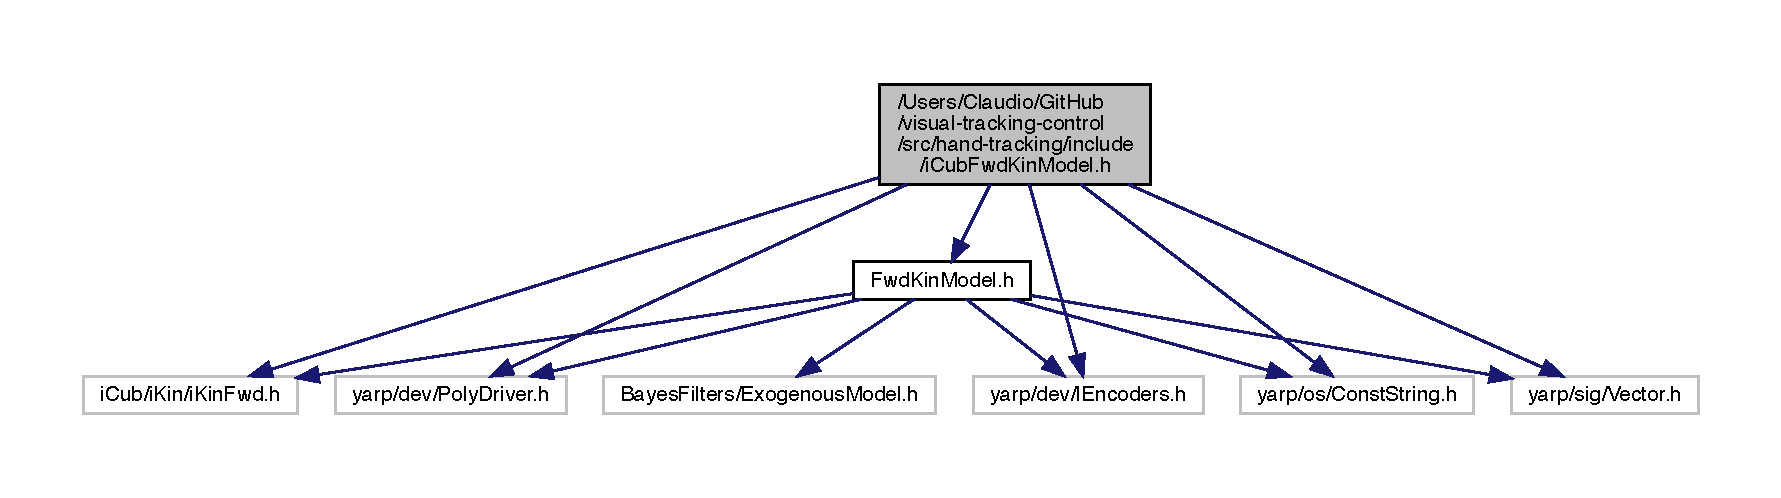
\includegraphics[width=350pt]{iCubFwdKinModel_8h__incl}
\end{center}
\end{figure}
This graph shows which files directly or indirectly include this file\+:
\nopagebreak
\begin{figure}[H]
\begin{center}
\leavevmode
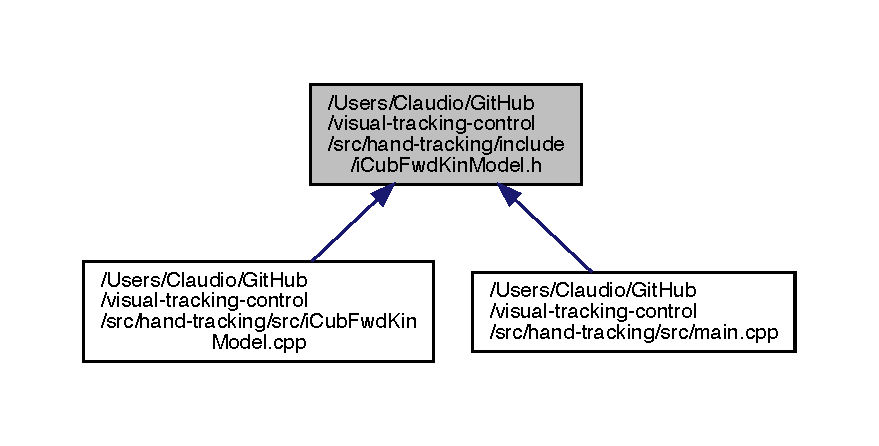
\includegraphics[width=350pt]{iCubFwdKinModel_8h__dep__incl}
\end{center}
\end{figure}
\subsection*{Classes}
\begin{DoxyCompactItemize}
\item 
class \hyperlink{classiCubFwdKinModel}{i\+Cub\+Fwd\+Kin\+Model}
\end{DoxyCompactItemize}

\hypertarget{iCubGatePose_8h}{}\section{/\+Users/\+Claudio/\+Git\+Hub/visual-\/tracking-\/control/src/hand-\/tracking/include/i\+Cub\+Gate\+Pose.h File Reference}
\label{iCubGatePose_8h}\index{/\+Users/\+Claudio/\+Git\+Hub/visual-\/tracking-\/control/src/hand-\/tracking/include/i\+Cub\+Gate\+Pose.\+h@{/\+Users/\+Claudio/\+Git\+Hub/visual-\/tracking-\/control/src/hand-\/tracking/include/i\+Cub\+Gate\+Pose.\+h}}
{\ttfamily \#include $<$Gate\+Pose.\+h$>$}\newline
{\ttfamily \#include $<$i\+Cub/i\+Kin/i\+Kin\+Fwd.\+h$>$}\newline
{\ttfamily \#include $<$yarp/dev/\+I\+Encoders.\+h$>$}\newline
{\ttfamily \#include $<$yarp/dev/\+Poly\+Driver.\+h$>$}\newline
{\ttfamily \#include $<$yarp/os/\+Const\+String.\+h$>$}\newline
{\ttfamily \#include $<$yarp/sig/\+Vector.\+h$>$}\newline
Include dependency graph for i\+Cub\+Gate\+Pose.\+h\+:
\nopagebreak
\begin{figure}[H]
\begin{center}
\leavevmode
\includegraphics[width=350pt]{iCubGatePose_8h__incl}
\end{center}
\end{figure}
This graph shows which files directly or indirectly include this file\+:
\nopagebreak
\begin{figure}[H]
\begin{center}
\leavevmode
\includegraphics[width=350pt]{iCubGatePose_8h__dep__incl}
\end{center}
\end{figure}
\subsection*{Classes}
\begin{DoxyCompactItemize}
\item 
class \hyperlink{classiCubGatePose}{i\+Cub\+Gate\+Pose}
\end{DoxyCompactItemize}

\hypertarget{InitiCubArm_8h}{}\section{/\+Users/\+Claudio/\+Git\+Hub/visual-\/tracking-\/control/src/hand-\/tracking/include/\+Initi\+Cub\+Arm.h File Reference}
\label{InitiCubArm_8h}\index{/\+Users/\+Claudio/\+Git\+Hub/visual-\/tracking-\/control/src/hand-\/tracking/include/\+Initi\+Cub\+Arm.\+h@{/\+Users/\+Claudio/\+Git\+Hub/visual-\/tracking-\/control/src/hand-\/tracking/include/\+Initi\+Cub\+Arm.\+h}}
{\ttfamily \#include $<$Bayes\+Filters/\+Initialization.\+h$>$}\newline
{\ttfamily \#include $<$i\+Cub/i\+Kin/i\+Kin\+Fwd.\+h$>$}\newline
{\ttfamily \#include $<$yarp/os/\+Bottle.\+h$>$}\newline
{\ttfamily \#include $<$yarp/os/\+Buffered\+Port.\+h$>$}\newline
{\ttfamily \#include $<$yarp/os/\+Const\+String.\+h$>$}\newline
{\ttfamily \#include $<$yarp/sig/\+Vector.\+h$>$}\newline
Include dependency graph for Initi\+Cub\+Arm.\+h\+:
\nopagebreak
\begin{figure}[H]
\begin{center}
\leavevmode
\includegraphics[width=350pt]{InitiCubArm_8h__incl}
\end{center}
\end{figure}
This graph shows which files directly or indirectly include this file\+:
\nopagebreak
\begin{figure}[H]
\begin{center}
\leavevmode
\includegraphics[width=350pt]{InitiCubArm_8h__dep__incl}
\end{center}
\end{figure}
\subsection*{Classes}
\begin{DoxyCompactItemize}
\item 
class \hyperlink{classInitiCubArm}{Initi\+Cub\+Arm}
\end{DoxyCompactItemize}

\hypertarget{PlayFwdKinModel_8h}{}\section{/\+Users/\+Claudio/\+Git\+Hub/visual-\/tracking-\/control/src/hand-\/tracking/include/\+Play\+Fwd\+Kin\+Model.h File Reference}
\label{PlayFwdKinModel_8h}\index{/\+Users/\+Claudio/\+Git\+Hub/visual-\/tracking-\/control/src/hand-\/tracking/include/\+Play\+Fwd\+Kin\+Model.\+h@{/\+Users/\+Claudio/\+Git\+Hub/visual-\/tracking-\/control/src/hand-\/tracking/include/\+Play\+Fwd\+Kin\+Model.\+h}}
{\ttfamily \#include $<$Fwd\+Kin\+Model.\+h$>$}\newline
{\ttfamily \#include $<$i\+Cub/i\+Kin/i\+Kin\+Fwd.\+h$>$}\newline
{\ttfamily \#include $<$yarp/os/\+Bottle.\+h$>$}\newline
{\ttfamily \#include $<$yarp/os/\+Buffered\+Port.\+h$>$}\newline
{\ttfamily \#include $<$yarp/os/\+Const\+String.\+h$>$}\newline
{\ttfamily \#include $<$yarp/sig/\+Vector.\+h$>$}\newline
Include dependency graph for Play\+Fwd\+Kin\+Model.\+h\+:
\nopagebreak
\begin{figure}[H]
\begin{center}
\leavevmode
\includegraphics[width=350pt]{PlayFwdKinModel_8h__incl}
\end{center}
\end{figure}
This graph shows which files directly or indirectly include this file\+:
\nopagebreak
\begin{figure}[H]
\begin{center}
\leavevmode
\includegraphics[width=350pt]{PlayFwdKinModel_8h__dep__incl}
\end{center}
\end{figure}
\subsection*{Classes}
\begin{DoxyCompactItemize}
\item 
class \hyperlink{classPlayFwdKinModel}{Play\+Fwd\+Kin\+Model}
\end{DoxyCompactItemize}

\hypertarget{PlayGatePose_8h}{}\section{/\+Users/\+Claudio/\+Git\+Hub/visual-\/tracking-\/control/src/hand-\/tracking/include/\+Play\+Gate\+Pose.h File Reference}
\label{PlayGatePose_8h}\index{/\+Users/\+Claudio/\+Git\+Hub/visual-\/tracking-\/control/src/hand-\/tracking/include/\+Play\+Gate\+Pose.\+h@{/\+Users/\+Claudio/\+Git\+Hub/visual-\/tracking-\/control/src/hand-\/tracking/include/\+Play\+Gate\+Pose.\+h}}
{\ttfamily \#include \char`\"{}Gate\+Pose.\+h\char`\"{}}\newline
{\ttfamily \#include $<$i\+Cub/i\+Kin/i\+Kin\+Fwd.\+h$>$}\newline
{\ttfamily \#include $<$yarp/os/\+Bottle.\+h$>$}\newline
{\ttfamily \#include $<$yarp/os/\+Buffered\+Port.\+h$>$}\newline
{\ttfamily \#include $<$yarp/sig/\+Vector.\+h$>$}\newline
Include dependency graph for Play\+Gate\+Pose.\+h\+:
\nopagebreak
\begin{figure}[H]
\begin{center}
\leavevmode
\includegraphics[width=350pt]{PlayGatePose_8h__incl}
\end{center}
\end{figure}
This graph shows which files directly or indirectly include this file\+:
\nopagebreak
\begin{figure}[H]
\begin{center}
\leavevmode
\includegraphics[width=350pt]{PlayGatePose_8h__dep__incl}
\end{center}
\end{figure}
\subsection*{Classes}
\begin{DoxyCompactItemize}
\item 
class \hyperlink{classPlayGatePose}{Play\+Gate\+Pose}
\end{DoxyCompactItemize}

\hypertarget{VisualProprioception_8h}{}\section{/\+Users/\+Claudio/\+Git\+Hub/visual-\/tracking-\/control/src/hand-\/tracking/include/\+Visual\+Proprioception.h File Reference}
\label{VisualProprioception_8h}\index{/\+Users/\+Claudio/\+Git\+Hub/visual-\/tracking-\/control/src/hand-\/tracking/include/\+Visual\+Proprioception.\+h@{/\+Users/\+Claudio/\+Git\+Hub/visual-\/tracking-\/control/src/hand-\/tracking/include/\+Visual\+Proprioception.\+h}}
{\ttfamily \#include $<$string$>$}\newline
{\ttfamily \#include $<$Bayes\+Filters/\+Visual\+Observation\+Model.\+h$>$}\newline
{\ttfamily \#include $<$i\+Cub/i\+Kin/i\+Kin\+Fwd.\+h$>$}\newline
{\ttfamily \#include $<$opencv2/core/core.\+hpp$>$}\newline
{\ttfamily \#include $<$Superimpose\+Mesh/\+S\+I\+C\+A\+D.\+h$>$}\newline
{\ttfamily \#include $<$yarp/dev/\+Gaze\+Control.\+h$>$}\newline
{\ttfamily \#include $<$yarp/dev/\+I\+Analog\+Sensor.\+h$>$}\newline
{\ttfamily \#include $<$yarp/dev/\+Poly\+Driver.\+h$>$}\newline
{\ttfamily \#include $<$yarp/os/\+Bottle.\+h$>$}\newline
{\ttfamily \#include $<$yarp/os/\+Buffered\+Port.\+h$>$}\newline
{\ttfamily \#include $<$yarp/os/\+Const\+String.\+h$>$}\newline
{\ttfamily \#include $<$yarp/sig/\+Matrix.\+h$>$}\newline
{\ttfamily \#include $<$yarp/sig/\+Vector.\+h$>$}\newline
Include dependency graph for Visual\+Proprioception.\+h\+:
\nopagebreak
\begin{figure}[H]
\begin{center}
\leavevmode
\includegraphics[width=350pt]{VisualProprioception_8h__incl}
\end{center}
\end{figure}
This graph shows which files directly or indirectly include this file\+:
\nopagebreak
\begin{figure}[H]
\begin{center}
\leavevmode
\includegraphics[width=350pt]{VisualProprioception_8h__dep__incl}
\end{center}
\end{figure}
\subsection*{Classes}
\begin{DoxyCompactItemize}
\item 
class \hyperlink{classVisualProprioception}{Visual\+Proprioception}
\end{DoxyCompactItemize}

\hypertarget{VisualSIS_8h}{}\section{/\+Users/\+Claudio/\+Git\+Hub/visual-\/tracking-\/control/src/hand-\/tracking/include/\+Visual\+S\+IS.h File Reference}
\label{VisualSIS_8h}\index{/\+Users/\+Claudio/\+Git\+Hub/visual-\/tracking-\/control/src/hand-\/tracking/include/\+Visual\+S\+I\+S.\+h@{/\+Users/\+Claudio/\+Git\+Hub/visual-\/tracking-\/control/src/hand-\/tracking/include/\+Visual\+S\+I\+S.\+h}}
{\ttfamily \#include $<$chrono$>$}\newline
{\ttfamily \#include $<$deque$>$}\newline
{\ttfamily \#include $<$memory$>$}\newline
{\ttfamily \#include $<$vector$>$}\newline
{\ttfamily \#include $<$Bayes\+Filters/\+Estimates\+Extraction.\+h$>$}\newline
{\ttfamily \#include $<$Bayes\+Filters/\+Visual\+Particle\+Filter.\+h$>$}\newline
{\ttfamily \#include $<$Eigen/\+Dense$>$}\newline
{\ttfamily \#include $<$i\+Cub/i\+Kin/i\+Kin\+Fwd.\+h$>$}\newline
{\ttfamily \#include $<$opencv2/cudaobjdetect.\+hpp$>$}\newline
{\ttfamily \#include $<$thrift/\+Visual\+S\+I\+S\+Particle\+Filter\+I\+D\+L.\+h$>$}\newline
{\ttfamily \#include $<$yarp/dev/\+Poly\+Driver.\+h$>$}\newline
{\ttfamily \#include $<$yarp/dev/\+I\+Analog\+Sensor.\+h$>$}\newline
{\ttfamily \#include $<$yarp/os/\+Bottle.\+h$>$}\newline
{\ttfamily \#include $<$yarp/os/\+Buffered\+Port.\+h$>$}\newline
{\ttfamily \#include $<$yarp/os/\+Const\+String.\+h$>$}\newline
{\ttfamily \#include $<$yarp/os/\+Port.\+h$>$}\newline
{\ttfamily \#include $<$yarp/sig/\+Image.\+h$>$}\newline
{\ttfamily \#include $<$yarp/sig/\+Matrix.\+h$>$}\newline
{\ttfamily \#include $<$yarp/sig/\+Vector.\+h$>$}\newline
Include dependency graph for Visual\+S\+I\+S.\+h\+:
\nopagebreak
\begin{figure}[H]
\begin{center}
\leavevmode
\includegraphics[width=350pt]{VisualSIS_8h__incl}
\end{center}
\end{figure}
This graph shows which files directly or indirectly include this file\+:
\nopagebreak
\begin{figure}[H]
\begin{center}
\leavevmode
\includegraphics[width=350pt]{VisualSIS_8h__dep__incl}
\end{center}
\end{figure}
\subsection*{Classes}
\begin{DoxyCompactItemize}
\item 
class \hyperlink{classVisualSIS}{Visual\+S\+IS}
\end{DoxyCompactItemize}

\hypertarget{VisualUpdateParticles_8h}{}\section{/\+Users/\+Claudio/\+Git\+Hub/visual-\/tracking-\/control/src/hand-\/tracking/include/\+Visual\+Update\+Particles.h File Reference}
\label{VisualUpdateParticles_8h}\index{/\+Users/\+Claudio/\+Git\+Hub/visual-\/tracking-\/control/src/hand-\/tracking/include/\+Visual\+Update\+Particles.\+h@{/\+Users/\+Claudio/\+Git\+Hub/visual-\/tracking-\/control/src/hand-\/tracking/include/\+Visual\+Update\+Particles.\+h}}
{\ttfamily \#include $<$Visual\+Proprioception.\+h$>$}\newline
{\ttfamily \#include $<$condition\+\_\+variable$>$}\newline
{\ttfamily \#include $<$mutex$>$}\newline
{\ttfamily \#include $<$thread$>$}\newline
{\ttfamily \#include $<$Bayes\+Filters/\+P\+F\+Visual\+Correction.\+h$>$}\newline
{\ttfamily \#include $<$opencv2/core/cuda.\+hpp$>$}\newline
{\ttfamily \#include $<$opencv2/cudaobjdetect.\+hpp$>$}\newline
{\ttfamily \#include $<$opencv2/objdetect/objdetect.\+hpp$>$}\newline
Include dependency graph for Visual\+Update\+Particles.\+h\+:
\nopagebreak
\begin{figure}[H]
\begin{center}
\leavevmode
\includegraphics[width=350pt]{VisualUpdateParticles_8h__incl}
\end{center}
\end{figure}
This graph shows which files directly or indirectly include this file\+:
\nopagebreak
\begin{figure}[H]
\begin{center}
\leavevmode
\includegraphics[width=350pt]{VisualUpdateParticles_8h__dep__incl}
\end{center}
\end{figure}
\subsection*{Classes}
\begin{DoxyCompactItemize}
\item 
class \hyperlink{classVisualUpdateParticles}{Visual\+Update\+Particles}
\end{DoxyCompactItemize}

\hypertarget{BrownianMotionPose_8cpp}{}\section{/\+Users/\+Claudio/\+Git\+Hub/visual-\/tracking-\/control/src/hand-\/tracking/src/\+Brownian\+Motion\+Pose.cpp File Reference}
\label{BrownianMotionPose_8cpp}\index{/\+Users/\+Claudio/\+Git\+Hub/visual-\/tracking-\/control/src/hand-\/tracking/src/\+Brownian\+Motion\+Pose.\+cpp@{/\+Users/\+Claudio/\+Git\+Hub/visual-\/tracking-\/control/src/hand-\/tracking/src/\+Brownian\+Motion\+Pose.\+cpp}}
{\ttfamily \#include $<$Brownian\+Motion\+Pose.\+h$>$}\newline
{\ttfamily \#include $<$cmath$>$}\newline
{\ttfamily \#include $<$iostream$>$}\newline
{\ttfamily \#include $<$utility$>$}\newline
Include dependency graph for Brownian\+Motion\+Pose.\+cpp\+:
\nopagebreak
\begin{figure}[H]
\begin{center}
\leavevmode
\includegraphics[width=350pt]{BrownianMotionPose_8cpp__incl}
\end{center}
\end{figure}

\hypertarget{DrawFwdKinPoses_8cpp}{}\section{/\+Users/\+Claudio/\+Git\+Hub/visual-\/tracking-\/control/src/hand-\/tracking/src/\+Draw\+Fwd\+Kin\+Poses.cpp File Reference}
\label{DrawFwdKinPoses_8cpp}\index{/\+Users/\+Claudio/\+Git\+Hub/visual-\/tracking-\/control/src/hand-\/tracking/src/\+Draw\+Fwd\+Kin\+Poses.\+cpp@{/\+Users/\+Claudio/\+Git\+Hub/visual-\/tracking-\/control/src/hand-\/tracking/src/\+Draw\+Fwd\+Kin\+Poses.\+cpp}}
{\ttfamily \#include $<$Draw\+Fwd\+Kin\+Poses.\+h$>$}\newline
{\ttfamily \#include $<$utility$>$}\newline
Include dependency graph for Draw\+Fwd\+Kin\+Poses.\+cpp\+:
\nopagebreak
\begin{figure}[H]
\begin{center}
\leavevmode
\includegraphics[width=350pt]{DrawFwdKinPoses_8cpp__incl}
\end{center}
\end{figure}

\hypertarget{FwdKinModel_8cpp}{}\section{/\+Users/\+Claudio/\+Git\+Hub/visual-\/tracking-\/control/src/hand-\/tracking/src/\+Fwd\+Kin\+Model.cpp File Reference}
\label{FwdKinModel_8cpp}\index{/\+Users/\+Claudio/\+Git\+Hub/visual-\/tracking-\/control/src/hand-\/tracking/src/\+Fwd\+Kin\+Model.\+cpp@{/\+Users/\+Claudio/\+Git\+Hub/visual-\/tracking-\/control/src/hand-\/tracking/src/\+Fwd\+Kin\+Model.\+cpp}}
{\ttfamily \#include $<$Fwd\+Kin\+Model.\+h$>$}\newline
{\ttfamily \#include $<$exception$>$}\newline
{\ttfamily \#include $<$iostream$>$}\newline
{\ttfamily \#include $<$functional$>$}\newline
{\ttfamily \#include $<$i\+Cub/ctrl/math.\+h$>$}\newline
{\ttfamily \#include $<$yarp/math/\+Math.\+h$>$}\newline
{\ttfamily \#include $<$yarp/os/\+Bottle.\+h$>$}\newline
{\ttfamily \#include $<$yarp/os/\+Property.\+h$>$}\newline
{\ttfamily \#include $<$yarp/os/\+Log\+Stream.\+h$>$}\newline
Include dependency graph for Fwd\+Kin\+Model.\+cpp\+:
\nopagebreak
\begin{figure}[H]
\begin{center}
\leavevmode
\includegraphics[width=350pt]{FwdKinModel_8cpp__incl}
\end{center}
\end{figure}

\hypertarget{GatePose_8cpp}{}\section{/\+Users/\+Claudio/\+Git\+Hub/visual-\/tracking-\/control/src/hand-\/tracking/src/\+Gate\+Pose.cpp File Reference}
\label{GatePose_8cpp}\index{/\+Users/\+Claudio/\+Git\+Hub/visual-\/tracking-\/control/src/hand-\/tracking/src/\+Gate\+Pose.\+cpp@{/\+Users/\+Claudio/\+Git\+Hub/visual-\/tracking-\/control/src/hand-\/tracking/src/\+Gate\+Pose.\+cpp}}
{\ttfamily \#include $<$Gate\+Pose.\+h$>$}\newline
{\ttfamily \#include $<$cmath$>$}\newline
Include dependency graph for Gate\+Pose.\+cpp\+:
\nopagebreak
\begin{figure}[H]
\begin{center}
\leavevmode
\includegraphics[width=350pt]{GatePose_8cpp__incl}
\end{center}
\end{figure}

\hypertarget{iCubFwdKinModel_8cpp}{}\section{/\+Users/\+Claudio/\+Git\+Hub/visual-\/tracking-\/control/src/hand-\/tracking/src/i\+Cub\+Fwd\+Kin\+Model.cpp File Reference}
\label{iCubFwdKinModel_8cpp}\index{/\+Users/\+Claudio/\+Git\+Hub/visual-\/tracking-\/control/src/hand-\/tracking/src/i\+Cub\+Fwd\+Kin\+Model.\+cpp@{/\+Users/\+Claudio/\+Git\+Hub/visual-\/tracking-\/control/src/hand-\/tracking/src/i\+Cub\+Fwd\+Kin\+Model.\+cpp}}
{\ttfamily \#include $<$i\+Cub\+Fwd\+Kin\+Model.\+h$>$}\newline
{\ttfamily \#include $<$exception$>$}\newline
{\ttfamily \#include $<$functional$>$}\newline
{\ttfamily \#include $<$i\+Cub/ctrl/math.\+h$>$}\newline
{\ttfamily \#include $<$yarp/eigen/\+Eigen.\+h$>$}\newline
{\ttfamily \#include $<$yarp/math/\+Math.\+h$>$}\newline
{\ttfamily \#include $<$yarp/os/\+Bottle.\+h$>$}\newline
{\ttfamily \#include $<$yarp/os/\+Property.\+h$>$}\newline
{\ttfamily \#include $<$yarp/os/\+Log\+Stream.\+h$>$}\newline
Include dependency graph for i\+Cub\+Fwd\+Kin\+Model.\+cpp\+:
\nopagebreak
\begin{figure}[H]
\begin{center}
\leavevmode
\includegraphics[width=350pt]{iCubFwdKinModel_8cpp__incl}
\end{center}
\end{figure}

\hypertarget{iCubGatePose_8cpp}{}\section{/\+Users/\+Claudio/\+Git\+Hub/visual-\/tracking-\/control/src/hand-\/tracking/src/i\+Cub\+Gate\+Pose.cpp File Reference}
\label{iCubGatePose_8cpp}\index{/\+Users/\+Claudio/\+Git\+Hub/visual-\/tracking-\/control/src/hand-\/tracking/src/i\+Cub\+Gate\+Pose.\+cpp@{/\+Users/\+Claudio/\+Git\+Hub/visual-\/tracking-\/control/src/hand-\/tracking/src/i\+Cub\+Gate\+Pose.\+cpp}}
{\ttfamily \#include $<$i\+Cub\+Gate\+Pose.\+h$>$}\newline
{\ttfamily \#include $<$i\+Cub/ctrl/math.\+h$>$}\newline
{\ttfamily \#include $<$yarp/eigen/\+Eigen.\+h$>$}\newline
{\ttfamily \#include $<$yarp/os/\+Log\+Stream.\+h$>$}\newline
{\ttfamily \#include $<$yarp/os/\+Property.\+h$>$}\newline
Include dependency graph for i\+Cub\+Gate\+Pose.\+cpp\+:
\nopagebreak
\begin{figure}[H]
\begin{center}
\leavevmode
\includegraphics[width=350pt]{iCubGatePose_8cpp__incl}
\end{center}
\end{figure}

\hypertarget{InitiCubArm_8cpp}{}\section{/\+Users/\+Claudio/\+Git\+Hub/visual-\/tracking-\/control/src/hand-\/tracking/src/\+Initi\+Cub\+Arm.cpp File Reference}
\label{InitiCubArm_8cpp}\index{/\+Users/\+Claudio/\+Git\+Hub/visual-\/tracking-\/control/src/hand-\/tracking/src/\+Initi\+Cub\+Arm.\+cpp@{/\+Users/\+Claudio/\+Git\+Hub/visual-\/tracking-\/control/src/hand-\/tracking/src/\+Initi\+Cub\+Arm.\+cpp}}
{\ttfamily \#include $<$Initi\+Cub\+Arm.\+h$>$}\newline
{\ttfamily \#include $<$i\+Cub/ctrl/math.\+h$>$}\newline
Include dependency graph for Initi\+Cub\+Arm.\+cpp\+:
\nopagebreak
\begin{figure}[H]
\begin{center}
\leavevmode
\includegraphics[width=350pt]{InitiCubArm_8cpp__incl}
\end{center}
\end{figure}

\hypertarget{hand-tracking_2src_2main_8cpp}{}\section{/\+Users/\+Claudio/\+Git\+Hub/visual-\/tracking-\/control/src/hand-\/tracking/src/main.cpp File Reference}
\label{hand-tracking_2src_2main_8cpp}\index{/\+Users/\+Claudio/\+Git\+Hub/visual-\/tracking-\/control/src/hand-\/tracking/src/main.\+cpp@{/\+Users/\+Claudio/\+Git\+Hub/visual-\/tracking-\/control/src/hand-\/tracking/src/main.\+cpp}}
{\ttfamily \#include $<$chrono$>$}\newline
{\ttfamily \#include $<$future$>$}\newline
{\ttfamily \#include $<$iostream$>$}\newline
{\ttfamily \#include $<$memory$>$}\newline
{\ttfamily \#include $<$Bayes\+Filters/\+Resampling\+With\+Prior.\+h$>$}\newline
{\ttfamily \#include $<$yarp/os/\+Const\+String.\+h$>$}\newline
{\ttfamily \#include $<$yarp/os/\+Log\+Stream.\+h$>$}\newline
{\ttfamily \#include $<$yarp/os/\+Network.\+h$>$}\newline
{\ttfamily \#include $<$yarp/os/\+Resource\+Finder.\+h$>$}\newline
{\ttfamily \#include $<$yarp/os/\+Value.\+h$>$}\newline
{\ttfamily \#include $<$opencv2/core/core.\+hpp$>$}\newline
{\ttfamily \#include $<$opencv2/core/cuda.\+hpp$>$}\newline
{\ttfamily \#include $<$Brownian\+Motion\+Pose.\+h$>$}\newline
{\ttfamily \#include $<$Draw\+Fwd\+Kin\+Poses.\+h$>$}\newline
{\ttfamily \#include $<$i\+Cub\+Gate\+Pose.\+h$>$}\newline
{\ttfamily \#include $<$i\+Cub\+Fwd\+Kin\+Model.\+h$>$}\newline
{\ttfamily \#include $<$Initi\+Cub\+Arm.\+h$>$}\newline
{\ttfamily \#include $<$Play\+Fwd\+Kin\+Model.\+h$>$}\newline
{\ttfamily \#include $<$Play\+Gate\+Pose.\+h$>$}\newline
{\ttfamily \#include $<$Visual\+Proprioception.\+h$>$}\newline
{\ttfamily \#include $<$Visual\+S\+I\+S.\+h$>$}\newline
{\ttfamily \#include $<$Visual\+Update\+Particles.\+h$>$}\newline
Include dependency graph for main.\+cpp\+:
\nopagebreak
\begin{figure}[H]
\begin{center}
\leavevmode
\includegraphics[width=350pt]{hand-tracking_2src_2main_8cpp__incl}
\end{center}
\end{figure}
\subsection*{Functions}
\begin{DoxyCompactItemize}
\item 
std\+::string \hyperlink{hand-tracking_2src_2main_8cpp_ae7defd726cf4a6ff613e0eba03121301}{engine\+\_\+count\+\_\+to\+\_\+string} (int engine\+\_\+count)
\item 
int \hyperlink{hand-tracking_2src_2main_8cpp_a0ddf1224851353fc92bfbff6f499fa97}{main} (int argc, char $\ast$argv\mbox{[}$\,$\mbox{]})
\end{DoxyCompactItemize}


\subsection{Function Documentation}
\mbox{\Hypertarget{hand-tracking_2src_2main_8cpp_ae7defd726cf4a6ff613e0eba03121301}\label{hand-tracking_2src_2main_8cpp_ae7defd726cf4a6ff613e0eba03121301}} 
\index{hand-\/tracking/src/main.\+cpp@{hand-\/tracking/src/main.\+cpp}!engine\+\_\+count\+\_\+to\+\_\+string@{engine\+\_\+count\+\_\+to\+\_\+string}}
\index{engine\+\_\+count\+\_\+to\+\_\+string@{engine\+\_\+count\+\_\+to\+\_\+string}!hand-\/tracking/src/main.\+cpp@{hand-\/tracking/src/main.\+cpp}}
\subsubsection{\texorpdfstring{engine\+\_\+count\+\_\+to\+\_\+string()}{engine\_count\_to\_string()}}
{\footnotesize\ttfamily std\+::string engine\+\_\+count\+\_\+to\+\_\+string (\begin{DoxyParamCaption}\item[{int}]{engine\+\_\+count }\end{DoxyParamCaption})}



Definition at line 256 of file main.\+cpp.



Referenced by main().

\mbox{\Hypertarget{hand-tracking_2src_2main_8cpp_a0ddf1224851353fc92bfbff6f499fa97}\label{hand-tracking_2src_2main_8cpp_a0ddf1224851353fc92bfbff6f499fa97}} 
\index{hand-\/tracking/src/main.\+cpp@{hand-\/tracking/src/main.\+cpp}!main@{main}}
\index{main@{main}!hand-\/tracking/src/main.\+cpp@{hand-\/tracking/src/main.\+cpp}}
\subsubsection{\texorpdfstring{main()}{main()}}
{\footnotesize\ttfamily int main (\begin{DoxyParamCaption}\item[{int}]{argc,  }\item[{char $\ast$}]{argv\mbox{[}$\,$\mbox{]} }\end{DoxyParamCaption})}



Definition at line 38 of file main.\+cpp.



References engine\+\_\+count\+\_\+to\+\_\+string().

Here is the call graph for this function\+:
\nopagebreak
\begin{figure}[H]
\begin{center}
\leavevmode
\includegraphics[width=274pt]{hand-tracking_2src_2main_8cpp_a0ddf1224851353fc92bfbff6f499fa97_cgraph}
\end{center}
\end{figure}

\hypertarget{reaching_2main_8cpp}{}\section{/\+Users/\+Claudio/\+Git\+Hub/visual-\/tracking-\/control/src/reaching/main.cpp File Reference}
\label{reaching_2main_8cpp}\index{/\+Users/\+Claudio/\+Git\+Hub/visual-\/tracking-\/control/src/reaching/main.\+cpp@{/\+Users/\+Claudio/\+Git\+Hub/visual-\/tracking-\/control/src/reaching/main.\+cpp}}
{\ttfamily \#include $<$cmath$>$}\newline
{\ttfamily \#include $<$iostream$>$}\newline
{\ttfamily \#include $<$i\+Cub/ctrl/min\+Jerk\+Ctrl.\+h$>$}\newline
{\ttfamily \#include $<$i\+Cub/i\+Kin/i\+Kin\+Fwd.\+h$>$}\newline
{\ttfamily \#include $<$opencv2/core/core.\+hpp$>$}\newline
{\ttfamily \#include $<$opencv2/imgproc/imgproc.\+hpp$>$}\newline
{\ttfamily \#include $<$Superimpose\+Mesh/\+S\+I\+Skeleton.\+h$>$}\newline
{\ttfamily \#include $<$yarp/dev/\+Cartesian\+Control.\+h$>$}\newline
{\ttfamily \#include $<$yarp/dev/\+Gaze\+Control.\+h$>$}\newline
{\ttfamily \#include $<$yarp/dev/\+Poly\+Driver.\+h$>$}\newline
{\ttfamily \#include $<$yarp/math/\+Math.\+h$>$}\newline
{\ttfamily \#include $<$yarp/math/\+S\+V\+D.\+h$>$}\newline
{\ttfamily \#include $<$yarp/os/\+Buffered\+Port.\+h$>$}\newline
{\ttfamily \#include $<$yarp/os/\+Log\+Stream.\+h$>$}\newline
{\ttfamily \#include $<$yarp/os/\+Network.\+h$>$}\newline
{\ttfamily \#include $<$yarp/os/\+Property.\+h$>$}\newline
{\ttfamily \#include $<$yarp/os/\+R\+F\+Module.\+h$>$}\newline
{\ttfamily \#include $<$yarp/os/\+Rpc\+Client.\+h$>$}\newline
{\ttfamily \#include $<$yarp/os/\+Time.\+h$>$}\newline
{\ttfamily \#include $<$yarp/sig/\+Image.\+h$>$}\newline
{\ttfamily \#include $<$yarp/sig/\+Matrix.\+h$>$}\newline
{\ttfamily \#include $<$yarp/sig/\+Vector.\+h$>$}\newline
Include dependency graph for main.\+cpp\+:
\nopagebreak
\begin{figure}[H]
\begin{center}
\leavevmode
\includegraphics[width=350pt]{reaching_2main_8cpp__incl}
\end{center}
\end{figure}
\subsection*{Classes}
\begin{DoxyCompactItemize}
\item 
class \hyperlink{classRFMReaching}{R\+F\+M\+Reaching}
\end{DoxyCompactItemize}
\subsection*{Functions}
\begin{DoxyCompactItemize}
\item 
int \hyperlink{reaching_2main_8cpp_ae66f6b31b5ad750f1fe042a706a4e3d4}{main} ()
\end{DoxyCompactItemize}


\subsection{Function Documentation}
\mbox{\Hypertarget{reaching_2main_8cpp_ae66f6b31b5ad750f1fe042a706a4e3d4}\label{reaching_2main_8cpp_ae66f6b31b5ad750f1fe042a706a4e3d4}} 
\index{reaching/main.\+cpp@{reaching/main.\+cpp}!main@{main}}
\index{main@{main}!reaching/main.\+cpp@{reaching/main.\+cpp}}
\subsubsection{\texorpdfstring{main()}{main()}}
{\footnotesize\ttfamily int main (\begin{DoxyParamCaption}{ }\end{DoxyParamCaption})}



Definition at line 1208 of file main.\+cpp.


\hypertarget{visualservoing_2visualservoingclient-app_2src_2main_8cpp}{}\section{/\+Users/\+Claudio/\+Git\+Hub/visual-\/tracking-\/control/src/visualservoing/visualservoingclient-\/app/src/main.cpp File Reference}
\label{visualservoing_2visualservoingclient-app_2src_2main_8cpp}\index{/\+Users/\+Claudio/\+Git\+Hub/visual-\/tracking-\/control/src/visualservoing/visualservoingclient-\/app/src/main.\+cpp@{/\+Users/\+Claudio/\+Git\+Hub/visual-\/tracking-\/control/src/visualservoing/visualservoingclient-\/app/src/main.\+cpp}}
{\ttfamily \#include $<$yarp/os/\+Log\+Stream.\+h$>$}\newline
{\ttfamily \#include $<$yarp/os/\+Property.\+h$>$}\newline
{\ttfamily \#include $<$yarp/dev/\+Drivers.\+h$>$}\newline
{\ttfamily \#include $<$yarp/dev/\+I\+Visual\+Servoing.\+h$>$}\newline
{\ttfamily \#include $<$yarp/dev/\+Poly\+Driver.\+h$>$}\newline
{\ttfamily \#include $<$yarp/math/\+Math.\+h$>$}\newline
Include dependency graph for main.\+cpp\+:
\nopagebreak
\begin{figure}[H]
\begin{center}
\leavevmode
\includegraphics[width=350pt]{visualservoing_2visualservoingclient-app_2src_2main_8cpp__incl}
\end{center}
\end{figure}
\subsection*{Functions}
\begin{DoxyCompactItemize}
\item 
\hyperlink{visualservoing_2visualservoingclient-app_2src_2main_8cpp_ab543f1556358acb521438f7c30e19de2}{Y\+A\+R\+P\+\_\+\+D\+E\+C\+L\+A\+R\+E\+\_\+\+P\+L\+U\+G\+I\+NS} (visualservoingplugin)
\item 
int \hyperlink{visualservoing_2visualservoingclient-app_2src_2main_8cpp_a3c04138a5bfe5d72780bb7e82a18e627}{main} (int argc, char $\ast$$\ast$argv)
\end{DoxyCompactItemize}


\subsection{Function Documentation}
\mbox{\Hypertarget{visualservoing_2visualservoingclient-app_2src_2main_8cpp_a3c04138a5bfe5d72780bb7e82a18e627}\label{visualservoing_2visualservoingclient-app_2src_2main_8cpp_a3c04138a5bfe5d72780bb7e82a18e627}} 
\index{visualservoing/visualservoingclient-\/app/src/main.\+cpp@{visualservoing/visualservoingclient-\/app/src/main.\+cpp}!main@{main}}
\index{main@{main}!visualservoing/visualservoingclient-\/app/src/main.\+cpp@{visualservoing/visualservoingclient-\/app/src/main.\+cpp}}
\subsubsection{\texorpdfstring{main()}{main()}}
{\footnotesize\ttfamily int main (\begin{DoxyParamCaption}\item[{int}]{argc,  }\item[{char $\ast$$\ast$}]{argv }\end{DoxyParamCaption})}



Definition at line 15 of file main.\+cpp.

\mbox{\Hypertarget{visualservoing_2visualservoingclient-app_2src_2main_8cpp_ab543f1556358acb521438f7c30e19de2}\label{visualservoing_2visualservoingclient-app_2src_2main_8cpp_ab543f1556358acb521438f7c30e19de2}} 
\index{visualservoing/visualservoingclient-\/app/src/main.\+cpp@{visualservoing/visualservoingclient-\/app/src/main.\+cpp}!Y\+A\+R\+P\+\_\+\+D\+E\+C\+L\+A\+R\+E\+\_\+\+P\+L\+U\+G\+I\+NS@{Y\+A\+R\+P\+\_\+\+D\+E\+C\+L\+A\+R\+E\+\_\+\+P\+L\+U\+G\+I\+NS}}
\index{Y\+A\+R\+P\+\_\+\+D\+E\+C\+L\+A\+R\+E\+\_\+\+P\+L\+U\+G\+I\+NS@{Y\+A\+R\+P\+\_\+\+D\+E\+C\+L\+A\+R\+E\+\_\+\+P\+L\+U\+G\+I\+NS}!visualservoing/visualservoingclient-\/app/src/main.\+cpp@{visualservoing/visualservoingclient-\/app/src/main.\+cpp}}
\subsubsection{\texorpdfstring{Y\+A\+R\+P\+\_\+\+D\+E\+C\+L\+A\+R\+E\+\_\+\+P\+L\+U\+G\+I\+N\+S()}{YARP\_DECLARE\_PLUGINS()}}
{\footnotesize\ttfamily Y\+A\+R\+P\+\_\+\+D\+E\+C\+L\+A\+R\+E\+\_\+\+P\+L\+U\+G\+I\+NS (\begin{DoxyParamCaption}\item[{visualservoingplugin}]{ }\end{DoxyParamCaption})}


\hypertarget{visualservoing_2visualservoingserver-app_2src_2main_8cpp}{}\section{/\+Users/\+Claudio/\+Git\+Hub/visual-\/tracking-\/control/src/visualservoing/visualservoingserver-\/app/src/main.cpp File Reference}
\label{visualservoing_2visualservoingserver-app_2src_2main_8cpp}\index{/\+Users/\+Claudio/\+Git\+Hub/visual-\/tracking-\/control/src/visualservoing/visualservoingserver-\/app/src/main.\+cpp@{/\+Users/\+Claudio/\+Git\+Hub/visual-\/tracking-\/control/src/visualservoing/visualservoingserver-\/app/src/main.\+cpp}}
{\ttfamily \#include $<$yarp/os/\+Log\+Stream.\+h$>$}\newline
{\ttfamily \#include $<$yarp/os/\+Property.\+h$>$}\newline
{\ttfamily \#include $<$yarp/dev/\+Drivers.\+h$>$}\newline
{\ttfamily \#include $<$yarp/dev/\+I\+Visual\+Servoing.\+h$>$}\newline
{\ttfamily \#include $<$yarp/dev/\+Poly\+Driver.\+h$>$}\newline
{\ttfamily \#include $<$yarp/math/\+Math.\+h$>$}\newline
Include dependency graph for main.\+cpp\+:
\nopagebreak
\begin{figure}[H]
\begin{center}
\leavevmode
\includegraphics[width=350pt]{visualservoing_2visualservoingserver-app_2src_2main_8cpp__incl}
\end{center}
\end{figure}
\subsection*{Functions}
\begin{DoxyCompactItemize}
\item 
\hyperlink{visualservoing_2visualservoingserver-app_2src_2main_8cpp_ab543f1556358acb521438f7c30e19de2}{Y\+A\+R\+P\+\_\+\+D\+E\+C\+L\+A\+R\+E\+\_\+\+P\+L\+U\+G\+I\+NS} (visualservoingplugin)
\item 
int \hyperlink{visualservoing_2visualservoingserver-app_2src_2main_8cpp_a3c04138a5bfe5d72780bb7e82a18e627}{main} (int argc, char $\ast$$\ast$argv)
\end{DoxyCompactItemize}


\subsection{Function Documentation}
\mbox{\Hypertarget{visualservoing_2visualservoingserver-app_2src_2main_8cpp_a3c04138a5bfe5d72780bb7e82a18e627}\label{visualservoing_2visualservoingserver-app_2src_2main_8cpp_a3c04138a5bfe5d72780bb7e82a18e627}} 
\index{visualservoing/visualservoingserver-\/app/src/main.\+cpp@{visualservoing/visualservoingserver-\/app/src/main.\+cpp}!main@{main}}
\index{main@{main}!visualservoing/visualservoingserver-\/app/src/main.\+cpp@{visualservoing/visualservoingserver-\/app/src/main.\+cpp}}
\subsubsection{\texorpdfstring{main()}{main()}}
{\footnotesize\ttfamily int main (\begin{DoxyParamCaption}\item[{int}]{argc,  }\item[{char $\ast$$\ast$}]{argv }\end{DoxyParamCaption})}



Definition at line 15 of file main.\+cpp.

\mbox{\Hypertarget{visualservoing_2visualservoingserver-app_2src_2main_8cpp_ab543f1556358acb521438f7c30e19de2}\label{visualservoing_2visualservoingserver-app_2src_2main_8cpp_ab543f1556358acb521438f7c30e19de2}} 
\index{visualservoing/visualservoingserver-\/app/src/main.\+cpp@{visualservoing/visualservoingserver-\/app/src/main.\+cpp}!Y\+A\+R\+P\+\_\+\+D\+E\+C\+L\+A\+R\+E\+\_\+\+P\+L\+U\+G\+I\+NS@{Y\+A\+R\+P\+\_\+\+D\+E\+C\+L\+A\+R\+E\+\_\+\+P\+L\+U\+G\+I\+NS}}
\index{Y\+A\+R\+P\+\_\+\+D\+E\+C\+L\+A\+R\+E\+\_\+\+P\+L\+U\+G\+I\+NS@{Y\+A\+R\+P\+\_\+\+D\+E\+C\+L\+A\+R\+E\+\_\+\+P\+L\+U\+G\+I\+NS}!visualservoing/visualservoingserver-\/app/src/main.\+cpp@{visualservoing/visualservoingserver-\/app/src/main.\+cpp}}
\subsubsection{\texorpdfstring{Y\+A\+R\+P\+\_\+\+D\+E\+C\+L\+A\+R\+E\+\_\+\+P\+L\+U\+G\+I\+N\+S()}{YARP\_DECLARE\_PLUGINS()}}
{\footnotesize\ttfamily Y\+A\+R\+P\+\_\+\+D\+E\+C\+L\+A\+R\+E\+\_\+\+P\+L\+U\+G\+I\+NS (\begin{DoxyParamCaption}\item[{visualservoingplugin}]{ }\end{DoxyParamCaption})}


\hypertarget{PlayFwdKinModel_8cpp}{}\section{/\+Users/\+Claudio/\+Git\+Hub/visual-\/tracking-\/control/src/hand-\/tracking/src/\+Play\+Fwd\+Kin\+Model.cpp File Reference}
\label{PlayFwdKinModel_8cpp}\index{/\+Users/\+Claudio/\+Git\+Hub/visual-\/tracking-\/control/src/hand-\/tracking/src/\+Play\+Fwd\+Kin\+Model.\+cpp@{/\+Users/\+Claudio/\+Git\+Hub/visual-\/tracking-\/control/src/hand-\/tracking/src/\+Play\+Fwd\+Kin\+Model.\+cpp}}
{\ttfamily \#include $<$Play\+Fwd\+Kin\+Model.\+h$>$}\newline
{\ttfamily \#include $<$exception$>$}\newline
{\ttfamily \#include $<$functional$>$}\newline
{\ttfamily \#include $<$i\+Cub/ctrl/math.\+h$>$}\newline
{\ttfamily \#include $<$yarp/math/\+Math.\+h$>$}\newline
{\ttfamily \#include $<$yarp/eigen/\+Eigen.\+h$>$}\newline
{\ttfamily \#include $<$yarp/os/\+Bottle.\+h$>$}\newline
{\ttfamily \#include $<$yarp/os/\+Property.\+h$>$}\newline
{\ttfamily \#include $<$yarp/os/\+Log\+Stream.\+h$>$}\newline
Include dependency graph for Play\+Fwd\+Kin\+Model.\+cpp\+:
\nopagebreak
\begin{figure}[H]
\begin{center}
\leavevmode
\includegraphics[width=350pt]{PlayFwdKinModel_8cpp__incl}
\end{center}
\end{figure}

\hypertarget{PlayGatePose_8cpp}{}\section{/\+Users/\+Claudio/\+Git\+Hub/visual-\/tracking-\/control/src/hand-\/tracking/src/\+Play\+Gate\+Pose.cpp File Reference}
\label{PlayGatePose_8cpp}\index{/\+Users/\+Claudio/\+Git\+Hub/visual-\/tracking-\/control/src/hand-\/tracking/src/\+Play\+Gate\+Pose.\+cpp@{/\+Users/\+Claudio/\+Git\+Hub/visual-\/tracking-\/control/src/hand-\/tracking/src/\+Play\+Gate\+Pose.\+cpp}}
{\ttfamily \#include $<$Play\+Gate\+Pose.\+h$>$}\newline
{\ttfamily \#include $<$i\+Cub/ctrl/math.\+h$>$}\newline
{\ttfamily \#include $<$yarp/eigen/\+Eigen.\+h$>$}\newline
{\ttfamily \#include $<$yarp/os/\+Log\+Stream.\+h$>$}\newline
{\ttfamily \#include $<$yarp/os/\+Property.\+h$>$}\newline
Include dependency graph for Play\+Gate\+Pose.\+cpp\+:
\nopagebreak
\begin{figure}[H]
\begin{center}
\leavevmode
\includegraphics[width=350pt]{PlayGatePose_8cpp__incl}
\end{center}
\end{figure}

\hypertarget{VisualProprioception_8cpp}{}\section{/\+Users/\+Claudio/\+Git\+Hub/visual-\/tracking-\/control/src/hand-\/tracking/src/\+Visual\+Proprioception.cpp File Reference}
\label{VisualProprioception_8cpp}\index{/\+Users/\+Claudio/\+Git\+Hub/visual-\/tracking-\/control/src/hand-\/tracking/src/\+Visual\+Proprioception.\+cpp@{/\+Users/\+Claudio/\+Git\+Hub/visual-\/tracking-\/control/src/hand-\/tracking/src/\+Visual\+Proprioception.\+cpp}}
{\ttfamily \#include $<$Visual\+Proprioception.\+h$>$}\newline
{\ttfamily \#include $<$cmath$>$}\newline
{\ttfamily \#include $<$exception$>$}\newline
{\ttfamily \#include $<$iostream$>$}\newline
{\ttfamily \#include $<$utility$>$}\newline
{\ttfamily \#include $<$i\+Cub/ctrl/math.\+h$>$}\newline
{\ttfamily \#include $<$yarp/math/\+Math.\+h$>$}\newline
{\ttfamily \#include $<$yarp/os/\+Log\+Stream.\+h$>$}\newline
{\ttfamily \#include $<$yarp/os/\+Property.\+h$>$}\newline
{\ttfamily \#include $<$yarp/os/\+Resource\+Finder.\+h$>$}\newline
Include dependency graph for Visual\+Proprioception.\+cpp\+:
\nopagebreak
\begin{figure}[H]
\begin{center}
\leavevmode
\includegraphics[width=350pt]{VisualProprioception_8cpp__incl}
\end{center}
\end{figure}

\hypertarget{VisualSIS_8cpp}{}\section{/\+Users/\+Claudio/\+Git\+Hub/visual-\/tracking-\/control/src/hand-\/tracking/src/\+Visual\+S\+IS.cpp File Reference}
\label{VisualSIS_8cpp}\index{/\+Users/\+Claudio/\+Git\+Hub/visual-\/tracking-\/control/src/hand-\/tracking/src/\+Visual\+S\+I\+S.\+cpp@{/\+Users/\+Claudio/\+Git\+Hub/visual-\/tracking-\/control/src/hand-\/tracking/src/\+Visual\+S\+I\+S.\+cpp}}
{\ttfamily \#include $<$Visual\+S\+I\+S.\+h$>$}\newline
{\ttfamily \#include $<$exception$>$}\newline
{\ttfamily \#include $<$iostream$>$}\newline
{\ttfamily \#include $<$utility$>$}\newline
{\ttfamily \#include $<$Eigen/\+Dense$>$}\newline
{\ttfamily \#include $<$i\+Cub/ctrl/math.\+h$>$}\newline
{\ttfamily \#include $<$opencv2/core/core.\+hpp$>$}\newline
{\ttfamily \#include $<$opencv2/core/cuda.\+hpp$>$}\newline
{\ttfamily \#include $<$opencv2/core/eigen.\+hpp$>$}\newline
{\ttfamily \#include $<$opencv2/imgproc/imgproc.\+hpp$>$}\newline
{\ttfamily \#include $<$opencv2/cudaimgproc.\+hpp$>$}\newline
{\ttfamily \#include $<$opencv2/cudawarping.\+hpp$>$}\newline
{\ttfamily \#include $<$yarp/eigen/\+Eigen.\+h$>$}\newline
{\ttfamily \#include $<$yarp/math/\+Math.\+h$>$}\newline
{\ttfamily \#include $<$yarp/os/\+Time.\+h$>$}\newline
Include dependency graph for Visual\+S\+I\+S.\+cpp\+:
\nopagebreak
\begin{figure}[H]
\begin{center}
\leavevmode
\includegraphics[width=350pt]{VisualSIS_8cpp__incl}
\end{center}
\end{figure}

\hypertarget{VisualUpdateParticles_8cpp}{}\section{/\+Users/\+Claudio/\+Git\+Hub/visual-\/tracking-\/control/src/hand-\/tracking/src/\+Visual\+Update\+Particles.cpp File Reference}
\label{VisualUpdateParticles_8cpp}\index{/\+Users/\+Claudio/\+Git\+Hub/visual-\/tracking-\/control/src/hand-\/tracking/src/\+Visual\+Update\+Particles.\+cpp@{/\+Users/\+Claudio/\+Git\+Hub/visual-\/tracking-\/control/src/hand-\/tracking/src/\+Visual\+Update\+Particles.\+cpp}}
{\ttfamily \#include $<$Visual\+Update\+Particles.\+h$>$}\newline
{\ttfamily \#include $<$cmath$>$}\newline
{\ttfamily \#include $<$exception$>$}\newline
{\ttfamily \#include $<$functional$>$}\newline
{\ttfamily \#include $<$iostream$>$}\newline
{\ttfamily \#include $<$utility$>$}\newline
{\ttfamily \#include $<$vector$>$}\newline
{\ttfamily \#include $<$opencv2/core/core.\+hpp$>$}\newline
{\ttfamily \#include $<$opencv2/core/cuda.\+hpp$>$}\newline
{\ttfamily \#include $<$opencv2/core/eigen.\+hpp$>$}\newline
{\ttfamily \#include $<$opencv2/cudaimgproc.\+hpp$>$}\newline
{\ttfamily \#include $<$opencv2/imgproc/imgproc.\+hpp$>$}\newline
Include dependency graph for Visual\+Update\+Particles.\+cpp\+:
\nopagebreak
\begin{figure}[H]
\begin{center}
\leavevmode
\includegraphics[width=350pt]{VisualUpdateParticles_8cpp__incl}
\end{center}
\end{figure}

\hypertarget{VisualServoingClient_8h}{}\section{/\+Users/\+Claudio/\+Git\+Hub/visual-\/tracking-\/control/src/visualservoing/visualservoingclient/include/\+Visual\+Servoing\+Client.h File Reference}
\label{VisualServoingClient_8h}\index{/\+Users/\+Claudio/\+Git\+Hub/visual-\/tracking-\/control/src/visualservoing/visualservoingclient/include/\+Visual\+Servoing\+Client.\+h@{/\+Users/\+Claudio/\+Git\+Hub/visual-\/tracking-\/control/src/visualservoing/visualservoingclient/include/\+Visual\+Servoing\+Client.\+h}}
{\ttfamily \#include \char`\"{}thrift/\+Visual\+Servoing\+I\+D\+L.\+h\char`\"{}}\newline
{\ttfamily \#include $<$vector$>$}\newline
{\ttfamily \#include $<$yarp/dev/\+Device\+Driver.\+h$>$}\newline
{\ttfamily \#include $<$yarp/dev/\+I\+Visual\+Servoing.\+h$>$}\newline
{\ttfamily \#include $<$yarp/os/\+Bottle.\+h$>$}\newline
{\ttfamily \#include $<$yarp/os/\+Buffered\+Port.\+h$>$}\newline
{\ttfamily \#include $<$yarp/os/\+Const\+String.\+h$>$}\newline
{\ttfamily \#include $<$yarp/os/\+Log\+Stream.\+h$>$}\newline
{\ttfamily \#include $<$yarp/os/\+Port.\+h$>$}\newline
{\ttfamily \#include $<$yarp/os/\+Searchable.\+h$>$}\newline
{\ttfamily \#include $<$yarp/sig/\+Vector.\+h$>$}\newline
Include dependency graph for Visual\+Servoing\+Client.\+h\+:
\nopagebreak
\begin{figure}[H]
\begin{center}
\leavevmode
\includegraphics[width=350pt]{VisualServoingClient_8h__incl}
\end{center}
\end{figure}
This graph shows which files directly or indirectly include this file\+:
\nopagebreak
\begin{figure}[H]
\begin{center}
\leavevmode
\includegraphics[width=268pt]{VisualServoingClient_8h__dep__incl}
\end{center}
\end{figure}
\subsection*{Classes}
\begin{DoxyCompactItemize}
\item 
class \hyperlink{classVisualServoingClient}{Visual\+Servoing\+Client}
\end{DoxyCompactItemize}

\hypertarget{VisualServoingClient_8cpp}{}\section{/\+Users/\+Claudio/\+Git\+Hub/visual-\/tracking-\/control/src/visualservoing/visualservoingclient/src/\+Visual\+Servoing\+Client.cpp File Reference}
\label{VisualServoingClient_8cpp}\index{/\+Users/\+Claudio/\+Git\+Hub/visual-\/tracking-\/control/src/visualservoing/visualservoingclient/src/\+Visual\+Servoing\+Client.\+cpp@{/\+Users/\+Claudio/\+Git\+Hub/visual-\/tracking-\/control/src/visualservoing/visualservoingclient/src/\+Visual\+Servoing\+Client.\+cpp}}
{\ttfamily \#include \char`\"{}Visual\+Servoing\+Client.\+h\char`\"{}}\newline
{\ttfamily \#include $<$i\+Cub/ctrl/min\+Jerk\+Ctrl.\+h$>$}\newline
{\ttfamily \#include $<$opencv2/core/core.\+hpp$>$}\newline
{\ttfamily \#include $<$opencv2/imgproc/imgproc.\+hpp$>$}\newline
{\ttfamily \#include $<$yarp/math/\+Math.\+h$>$}\newline
{\ttfamily \#include $<$yarp/math/\+S\+V\+D.\+h$>$}\newline
{\ttfamily \#include $<$yarp/os/\+Network.\+h$>$}\newline
{\ttfamily \#include $<$yarp/os/\+Property.\+h$>$}\newline
{\ttfamily \#include $<$yarp/os/\+Rpc\+Client.\+h$>$}\newline
{\ttfamily \#include $<$yarp/os/\+Time.\+h$>$}\newline
Include dependency graph for Visual\+Servoing\+Client.\+cpp\+:
\nopagebreak
\begin{figure}[H]
\begin{center}
\leavevmode
\includegraphics[width=350pt]{VisualServoingClient_8cpp__incl}
\end{center}
\end{figure}

\hypertarget{VisualServoingCommon_8h}{}\section{/\+Users/\+Claudio/\+Git\+Hub/visual-\/tracking-\/control/src/visualservoing/visualservoingcommon/include/\+Visual\+Servoing\+Common.h File Reference}
\label{VisualServoingCommon_8h}\index{/\+Users/\+Claudio/\+Git\+Hub/visual-\/tracking-\/control/src/visualservoing/visualservoingcommon/include/\+Visual\+Servoing\+Common.\+h@{/\+Users/\+Claudio/\+Git\+Hub/visual-\/tracking-\/control/src/visualservoing/visualservoingcommon/include/\+Visual\+Servoing\+Common.\+h}}

\hypertarget{VisualServoingServer_8h}{}\section{/\+Users/\+Claudio/\+Git\+Hub/visual-\/tracking-\/control/src/visualservoing/visualservoingserver/include/\+Visual\+Servoing\+Server.h File Reference}
\label{VisualServoingServer_8h}\index{/\+Users/\+Claudio/\+Git\+Hub/visual-\/tracking-\/control/src/visualservoing/visualservoingserver/include/\+Visual\+Servoing\+Server.\+h@{/\+Users/\+Claudio/\+Git\+Hub/visual-\/tracking-\/control/src/visualservoing/visualservoingserver/include/\+Visual\+Servoing\+Server.\+h}}
{\ttfamily \#include \char`\"{}thrift/\+Visual\+Servoing\+I\+D\+L.\+h\char`\"{}}\newline
{\ttfamily \#include $<$array$>$}\newline
{\ttfamily \#include $<$cmath$>$}\newline
{\ttfamily \#include $<$mutex$>$}\newline
{\ttfamily \#include $<$thread$>$}\newline
{\ttfamily \#include $<$vector$>$}\newline
{\ttfamily \#include $<$yarp/dev/\+Cartesian\+Control.\+h$>$}\newline
{\ttfamily \#include $<$yarp/dev/\+Gaze\+Control.\+h$>$}\newline
{\ttfamily \#include $<$yarp/dev/\+Device\+Driver.\+h$>$}\newline
{\ttfamily \#include $<$yarp/dev/\+I\+Encoders.\+h$>$}\newline
{\ttfamily \#include $<$yarp/dev/\+I\+Visual\+Servoing.\+h$>$}\newline
{\ttfamily \#include $<$yarp/dev/\+Poly\+Driver.\+h$>$}\newline
{\ttfamily \#include $<$yarp/math/\+Math.\+h$>$}\newline
{\ttfamily \#include $<$yarp/os/\+Bottle.\+h$>$}\newline
{\ttfamily \#include $<$yarp/os/\+Buffered\+Port.\+h$>$}\newline
{\ttfamily \#include $<$yarp/os/\+Const\+String.\+h$>$}\newline
{\ttfamily \#include $<$yarp/os/\+Log\+Stream.\+h$>$}\newline
{\ttfamily \#include $<$yarp/os/\+Port.\+h$>$}\newline
{\ttfamily \#include $<$yarp/os/\+Rpc\+Client.\+h$>$}\newline
{\ttfamily \#include $<$yarp/os/\+Thread.\+h$>$}\newline
{\ttfamily \#include $<$yarp/os/\+Searchable.\+h$>$}\newline
{\ttfamily \#include $<$yarp/sig/\+Image.\+h$>$}\newline
{\ttfamily \#include $<$yarp/sig/\+Matrix.\+h$>$}\newline
{\ttfamily \#include $<$yarp/sig/\+Vector.\+h$>$}\newline
Include dependency graph for Visual\+Servoing\+Server.\+h\+:
\nopagebreak
\begin{figure}[H]
\begin{center}
\leavevmode
\includegraphics[width=350pt]{VisualServoingServer_8h__incl}
\end{center}
\end{figure}
This graph shows which files directly or indirectly include this file\+:
\nopagebreak
\begin{figure}[H]
\begin{center}
\leavevmode
\includegraphics[width=272pt]{VisualServoingServer_8h__dep__incl}
\end{center}
\end{figure}
\subsection*{Classes}
\begin{DoxyCompactItemize}
\item 
class \hyperlink{classVisualServoingServer}{Visual\+Servoing\+Server}
\end{DoxyCompactItemize}

\hypertarget{VisualServoingServer_8cpp}{}\section{/\+Users/\+Claudio/\+Git\+Hub/visual-\/tracking-\/control/src/visualservoing/visualservoingserver/src/\+Visual\+Servoing\+Server.cpp File Reference}
\label{VisualServoingServer_8cpp}\index{/\+Users/\+Claudio/\+Git\+Hub/visual-\/tracking-\/control/src/visualservoing/visualservoingserver/src/\+Visual\+Servoing\+Server.\+cpp@{/\+Users/\+Claudio/\+Git\+Hub/visual-\/tracking-\/control/src/visualservoing/visualservoingserver/src/\+Visual\+Servoing\+Server.\+cpp}}
{\ttfamily \#include \char`\"{}Visual\+Servoing\+Server.\+h\char`\"{}}\newline
{\ttfamily \#include $<$i\+Cub/ctrl/min\+Jerk\+Ctrl.\+h$>$}\newline
{\ttfamily \#include $<$opencv2/core/core.\+hpp$>$}\newline
{\ttfamily \#include $<$opencv2/imgproc/imgproc.\+hpp$>$}\newline
{\ttfamily \#include $<$yarp/math/\+Math.\+h$>$}\newline
{\ttfamily \#include $<$yarp/math/\+S\+V\+D.\+h$>$}\newline
{\ttfamily \#include $<$yarp/os/\+Network.\+h$>$}\newline
{\ttfamily \#include $<$yarp/os/\+Property.\+h$>$}\newline
{\ttfamily \#include $<$yarp/os/\+Time.\+h$>$}\newline
Include dependency graph for Visual\+Servoing\+Server.\+cpp\+:
\nopagebreak
\begin{figure}[H]
\begin{center}
\leavevmode
\includegraphics[width=350pt]{VisualServoingServer_8cpp__incl}
\end{center}
\end{figure}

%--- End generated contents ---

% Index
\backmatter
\newpage
\phantomsection
\clearemptydoublepage
\addcontentsline{toc}{chapter}{Index}
\printindex

\end{document}
